  %-------------------------------------------------------------------------------
%
% TUM Dissertation Template
%
% For usage instructions see README.md
%
% Authors:
%   Andre Richter, andre.richter@tum.de
%   Michael Vonbun, michael.vonbun@tum.de
%   Christian Herber, christian.herber@tum.de
%   Stefan Wallentowitz, stefan.wallentowitz@tum.de
%
%-------------------------------------------------------------------------------
\documentclass[%
  % layouttitlepage,            % layout help rules (to see if you need
  %                             % some extra vspace in your title etc.)
  % headings = standardclasses, % serif fonts for headings
  % headings = big,             % If you use serif fonts for headings (above option
  %                             % uncommmented), uncomment this one to get smaller
  %                             % headings
  % sansseriftitlepage,         % sans serif title page
  % notocintoc,                 % do not add toc to toc itself
]{tumDiss}
\usepackage[utf8]{inputenc}



%-------------------------------------------------------------------------------
% Binding correction for the title page.
% WARNING: ONLY NEEDED FOR THE PRINT VERSION!
%
% After printing and binding, the left part of the titlepage may lose
% significant space, for example due to overlap from glue binding.
% You can increase the left margin of the title page with this option.
% This value of 8mm was measured for glue binding a thesis that was printed by
% the TUM Fachschaft EI and ~140 pages.
%-------------------------------------------------------------------------------
% \titlepagebindingcor{8mm}

%-------------------------------------------------------------------------------
% Binding correction for everything else.
% Does not affect titlePageBindingCor!
%
% WARNING: THIS OPTION CAN SHAKE UP YOUR CURRENT LAYOUT.
% If you want to use it, it is best to work with it from the very start. Adding
% it when finishing your dissertation might get you into trouble.
%
% Search http://texdoc.net/texmf-dist/doc/latex/koma-script/scrguien.pdf for
% "BCOR" for further reading.
%-------------------------------------------------------------------------------
% \KOMAoptions{BCOR=3mm}



%-------------------------------------------------------------------------------
% Faculty
%-------------------------------------------------------------------------------
\faculty{Fakultät für Informatik}

%-------------------------------------------------------------------------------
% Degree
%-------------------------------------------------------------------------------
\degree{Doktors der Naturwissenschaften (Dr. rer. nat.)}

%-------------------------------------------------------------------------------
% Title
%
% IMPORTANT:
%
% You must add manual line breaks here. If you don't, you'll get uneven spacing
% between the lines.
% YOU ALSO NEED THE BREAK AT THE LAST LINE.
%-------------------------------------------------------------------------------
\title{%
  Uncertainty Estimation\\ 
  for Independent and Non-Independent Data\\
}
% \subtitle{That is extended by using an additional subtitle}

%-------------------------------------------------------------------------------
% People
%-------------------------------------------------------------------------------
\author{Bertrand Charpentier}
\vorsitz[Technical University Munich]{Prof. Jens Großklags}
\erstpruef[Technical University Munich]{Prof. Dr. Stephan Günnemann}

% Use this one for a TUM professor
%\zweitpruef{Prof. Eyke Hüllermeier}

% Or this one for an external professor
\zweitpruef[Ludwig-Maximilians University]{Prof. Eyke Hüllermeier}
%% Eric Moulines
%% Emtiyaz Khan
%% Michael Bronstein
% Eyke Hüllermeier
% Mykel Kochenderfer
%% Vincent Fortuin
%% Daniel Cremers
% Matthias Hein
%% Philipp Hennig

% Optionally, add a third examiner
%\drittpruef[RWTH Aachen]{Prof. Dr.-Ing. Max Mustermann}

%-------------------------------------------------------------------------------
% Hand in date
%
% This is the date of your personal hand-in at the TUM doctoral office.
%-------------------------------------------------------------------------------
\date{01.01.2016}

%-------------------------------------------------------------------------------
% Accepted date
%
% You can set this after your thesis was accepted. For handing in,
% it is not needed (at least for the Electrical Engineering faculty).
%-------------------------------------------------------------------------------
\dateaccepted{10.05.2016}



%-------------------------------------------------------------------------------
% Change language, e.g. to german
%-------------------------------------------------------------------------------
% \usepackage[ngerman]{babel}

%-------------------------------------------------------------------------------
% Compatibility issues
%-------------------------------------------------------------------------------
% If you need pstricks, load it here before everything else.
% Otherwise, tikz patterns won't work
%\usepackage{pstricks}

%-------------------------------------------------------------------------------
% Suggested standard packets are included here
%-------------------------------------------------------------------------------
% Loading scrhack fixes:
%   (1) KOMA-Script incompatible macros used in listings package.
%   (2) Inconsistent anchors in hyperref.
\usepackage{scrhack}


% figure inclusion
\usepackage{amsthm}
%\usepackage[
%  caption = false,
%  font    = footnotesize
%]{subfig}
\usepackage{graphicx}
\usepackage{pgfplots}
\usepackage{pgfplotstable}
\usepackage[numbers]{natbib}
\tikzset{>=stealth}
\usetikzlibrary{patterns}
\usetikzlibrary{pgfplots.statistics}

\usepackage{tocloft}
\newlength\mylen
\renewcommand\cftpartpresnum{Part~}
\settowidth\mylen{\bfseries\cftpartpresnum\cftpartaftersnum}
\addtolength\cftpartnumwidth{\mylen}

% code block insertion
\usepackage{moreverb}
\usepackage{listings}

% math and equations
\usepackage{amsmath}
\usepackage{amssymb}
\usepackage{amsfonts}
\usepackage{upgreek}

% enumeration
\usepackage{enumerate}

\usepackage{booktabs} % For formal tables
\usepackage{xspace}
\usepackage{mathtools, cuted}
\usepackage{subcaption}
\usepackage{graphicx,caption}
\usepackage{wrapfig}
%\usepackage{arydshln}
\usepackage{floatflt}
\usepackage[ruled,vlined]{algorithm2e}
\usepackage{bm}
\usepackage{pgf}
\usepackage{makecell}
\usepackage{rotating, multirow}
\usepackage{tikz}
\usetikzlibrary{positioning}
\usetikzlibrary{backgrounds,matrix,patterns}
\usetikzlibrary{decorations.pathmorphing, patterns}
\definecolor{color0}{RGB}{220, 38, 127}
\definecolor{color1}{RGB}{100, 143, 255}
\definecolor{color2}{RGB}{254, 97, 0}
\definecolor{color3}{RGB}{120, 94, 240}
\definecolor{color4}{RGB}{255, 176, 0}

% Source code with highlighting
\usepackage{listings}
\lstset{
  basicstyle       = \footnotesize,
  captionpos       = b,
  tabsize          = 4,
  commentstyle     = \color{TUMGreen},
  keywordstyle     = \color{TUMBlue},
  stringstyle      = \color{TUMOrange},
  otherkeywords    = {
    uint64_t,
    uint32_t,
    uint16_t,
    uint8_t,
    u64,
    u32,
    u16,
    u8,
    inline
  },
  numbers          = left,
  xleftmargin      = 7ex,
  aboveskip        = 4ex,
  abovecaptionskip = 2ex,
}

% Support for siunitx
\usepackage{siunitx}
\sisetup{
  exponent-product = \cdot,
  output-product   = \cdot,
  per-mode         = symbol-or-fraction,
  quotient-mode    = fraction,
  binary-units     = true
}

% No widows and orphans
\usepackage[all]{nowidow}

% dummy text
\usepackage{lipsum}

% hyperlinks
% according to its documentation, hyperref should be loaded last
% a list of packages that should be loaded after hyperref can be found at
% https://tex.stackexchange.com/questions/1863/which-packages-should-be-loaded-after-hyperref-instead-of-before
\usepackage{url}
\usepackage[
  hidelinks,
  bookmarksnumbered,
]{hyperref}

% If hyperref is used, references to tables and figures link to their captions
% and not the actual tables or figures. This is especially unwanted for figures,
% because their captions are below the figure so that clicking on a link just
% shows the captions and the figure is invisible.
%
% Using the caption package fixes this behaviour.
\usepackage{caption}

% glossary functionality
% loading glossaries after hyperref adds hyperlings to acronyms and glossary
% entries
\usepackage[
  toc,
  acronym,
  style = long
]{glossaries}
\makeglossaries

%-------------------------------------------------------------------------------
% Include custom packages here
%-------------------------------------------------------------------------------

% \usepackage{}


%-------------------------------------------------------------------------------
% TUM CI colors for PGF
%-------------------------------------------------------------------------------
\definecolor{grey60} {RGB} {102, 102, 102} % 60% grey

%-------------------------------------------------------------------------------
% Default values for pgfplots
%-------------------------------------------------------------------------------
\newcommand{\figureHeight}{0.5625} %% 16:9
\pgfplotsset{
  compat           = 1.13,
  grid             = major,
  enlarge x limits = 0,
  cycle list name  = tum,
  major grid style = {dotted},
  minor grid style = {dotted},
  legend style     = {
    at     = {(0.98,0.96)},
    anchor = north east,
  },
  width            = \hsize * 0.9,
  height           = \hsize * 0.9 * \figureHeight,
}

%-------------------------------------------------------------------------------
% Correct bad hyphenation here
%-------------------------------------------------------------------------------
\hyphenation{op-tical net-works semi-conduc-tor}

%-------------------------------------------------------------------------------
% Acronyms (will be sorted alphabetically)
%-------------------------------------------------------------------------------
\newacronym{cpu}{CPU}{Central Processing Unit}
\glsadd{cpu}

\newacronym{pci}{PCI}{Peripheral Component Interconnect}
\glsadd{pci}

\newacronym{pcie}{PCIe}{Peripheral Component Interconnect Express}
\glsadd{pcie}

\newacronym{mmu}{MMU}{Memory Management Unit}
\glsadd{mmu}

\usepackage{float}
\usepackage[table]{colortbl}
\usepackage{nicefrac,xfrac}
\usepackage{bbm}
\usetikzlibrary{arrows}
\usepackage{pifont}
\usepackage{adjustbox}
% 006

\definecolor{Gray}{gray}{0.85}
\newcommand{\theHalgorithm}{\arabic{algorithm}}
\newcommand{\E}{\mathbb{E}}
\newcommand{\prob}{\mathbb{P}}
\newcommand{\Dir}{\mathrm{Dir}}
\newcommand{\Ber}{\mathrm{Ber}}
\newcommand{\Cat}{\mathrm{Cat}}
\newcommand{\Var}{\mathrm{Var}}
\newcommand{\Cov}{\mathrm{Cov}}
\newcommand\UCE{Uncertain Cross Entropy loss\xspace}
\newcommand\UCEacro{UCE\xspace}
\newcommand\ours{Posterior Network\xspace}
\newcommand\oursacro{PostNet\xspace}
\newcommand\SeqBn{Seq-Bn\xspace}
\newcommand\SeqNoBn{Seq-No-Bn\xspace}
\newcommand\NoFlow{No-Flow\xspace}
\newcommand\NoUCE{No-Bayes-Loss\xspace}
\newcommand\idata{i\xspace}
\newcommand\dataix{^{(\idata)}}
\newcommand\iclass{c\xspace}
\newcommand\nclass{C\xspace}
\newcommand\latent{\bold{z}}
\newcommand{\latentdim}{H}
\newtheorem{property}{Property}
\newtheorem{proposition}{Proposition}

% 007

\newcommand{\condition}{\ensuremath{\,|\,}}
\newcommand{\concat}{\ensuremath{\;||\;}}

\newcommand\NatPN{Natural Posterior Network}
\newcommand\NatPNacro{NatPN}

%% Math %%
% \newcommand\x{\bm{x}}
% \newcommand\z{\bm{z}}
\newcommand\expparam{\bm{\theta}}
\newcommand\priorparam{\bm{\chi}}
\newcommand\evidence{n}
% \newcommand\y{y}
\newcommand{\inputdim}{D}
% \newcommand{\latentdim}{H}
\newcommand{\suffstatdim}{L}
% \newcommand\idata{i\xspace}
\newcommand\ndata{N\xspace}
% \newcommand\dataix{^{(\idata)}}
% \newcommand\iclass{c\xspace}
% \newcommand\nclass{C\xspace}
\newtheorem{theorem}{Theorem}
\newtheorem*{theorem*}{Theorem}
\newtheorem{lemma}[theorem]{Lemma}

\DeclareMathOperator{\DCat}{Cat}
\DeclareMathOperator{\DDir}{Dir}
\DeclareMathOperator{\DBeta}{Beta}
\DeclareMathOperator{\DBer}{Ber}
\DeclareMathOperator{\DGamma}{\Gamma}
\DeclareMathOperator{\DNIG}{\mathcal{N}\Gamma^{-1}}
\DeclareMathOperator{\DNormal}{\mathcal{N}}
\DeclareMathOperator{\DPoi}{Poi}
\DeclareMathOperator{\corpus}{\mathbb{K}}
\DeclareMathOperator{\real}{\mathbb{R}}
\DeclareMathOperator{\posinteger}{\mathbb{N}}
% \DeclareMathOperator{\prob}{\mathbb{P}}
\DeclareMathOperator{\prior}{\mathbb{Q}}
\DeclareMathOperator{\entropy}{\mathbb{H}}
\DeclareMathOperator{\expectation}{\mathbb{E}}
\DeclareMathOperator{\variance}{Var}
\DeclareMathOperator{\loss}{\mathcal{L}}
\DeclareMathOperator{\data}{\mathcal{D}}
\DeclareMathOperator{\Enc}{Enc}
\DeclareMathOperator{\Dec}{Dec}
\DeclareMathOperator*{\argmin}{arg\,min}
\DeclareMathOperator*{\argmax}{arg\,max}

% 008

% \DeclareMathOperator{\DNormal}{\mathcal{N}}

% \newcommand\idata{i\xspace}
% \newcommand\dataix{^{(\idata)}}
% \newcommand\iclass{c\xspace}
% \newcommand\nclass{C\xspace}
\newcommand\PriorNet{PriorNet\xspace}
\newcommand\RevPriorNet{RevPriorNet\xspace}
\newcommand\EvNet{EvNet\xspace}
\newcommand\DDNet{DDNet\xspace}
\newcommand\PostNet{PostNet\xspace}

% 009

%% generic math notations %%
\newcommand{\rvar}[1]{\textnormal{#1}}
\newcommand{\rvec}[1]{\mathbf{#1}}
\newcommand{\rvecelem}[1]{\textnormal{#1}}
\newcommand{\rmat}[1]{\mathbf{#1}}
\newcommand{\rmatelem}[1]{\textnormal{#1}}
% vectors
\newcommand{\vect}[1]{\bm{#1}}
% matrices
\newcommand{\mat}[1]{\bm{#1}}
% entries of vectors are simply scalars
% entries of matrices are simply scalars
% sets
\newcommand{\set}[1]{\mathcal{#1}}


%% short-hand notations %%
% short-hand for epsilon
\def\eps{{\epsilon}}
% short-hand notations for vectors
\def\veczero{\vect{0}}
\def\vecone{\vect{1}}
\def\va{\vect{a}}
\def\ve{\vect{e}}
\def\vh{\vect{h}}
\def\vi{\vect{i}}
\def\vn{\vect{n}}
\def\vp{\vect{p}}
\def\vu{\vect{u}}
\def\vw{\vect{w}}
\def\vx{\vect{x}}
\def\vy{\vect{y}}
\def\vz{\vect{z}}
\def\valpha{\vect{\alpha}}
\def\vbeta{\vect{\beta}}
\def\vpi{\vect{\pi}}
\def\vpsi{\vect{\psi}}
\def\vphi{\vect{\phi}}
\def\vmu{\vect{\mu}}
\def\vtheta{\vect{\theta}}
\def\vomega{\vect{\omega}}
\def\vchi{\vect{\chi}}
% short-hand notation for matrices
\def\mA{\mat{A}}
\def\mE{\mat{E}}
\def\mH{\mat{H}}
\def\mI{\mat{I}}
\def\mW{\mat{W}}
\def\mX{\mat{X}}
\def\mY{\mat{Y}}
\def\mZ{\mat{Z}}
% short-hand notation for graphs
\def\sG{\set{G}}
\def\sN{\set{N}}
\def\sE{\set{E}}
\def\sU{\set{U}}
\def\sV{\set{V}}
\def\sY{\set{Y}}
\def\sL{\set{L}}
\def\sT{\set{T}}

\newcommand{\ExpecationArgs}[2]{\expectation_{#1}\left[#2\right]}

%% abbreviations %%
\newcommand\GPN{Graph Posterior Network}
\newcommand\GPNacro{GPN}

\newcommand\x{\vx}
\newcommand\z{\vz}
\newcommand\y{y}
\newcommand\p{\vp}
\newcommand\unc{u}
% \newcommand\expparam{\bm{\theta}}
% \newcommand\priorparam{\bm{\chi}}
% \newcommand\evidence{n}
\newcommand\genlatent{\vect{\zeta}}
\newcommand\suffstat{\bm{\chi}}
% \newcommand{\inputdim}{D}
% \newcommand{\latentdim}{H}
% \newcommand{\suffstatdim}{L}
\newcommand\nnodes{N}
\newcommand\nodeu{u}
\newcommand\nodev{v}
\newcommand\nodew{w}
\newcommand\noderepru{\hat{u}}
\newcommand\nodereprv{\hat{v}}
\newcommand\postnoderepru{\tilde{\hat{u}}}
\newcommand\postnodereprv{\tilde{\hat{v}}}
\newcommand\nodeidxu{^{(u)}}
\newcommand\nodeidxv{^{(v)}}
\newcommand\namednodeidxu[1]{^{#1, (u)}}
\newcommand\namednodeidxv[1]{^{#1, (v)}}
% \newcommand\iclass{c}
% \newcommand\nclass{C}
\newcommand\targets{\sY}
\newcommand\graph{\sG}
\newcommand\vertices{\sV}
\newcommand\edges{\sE}
\newcommand\neighbors{\sN}
\newcommand\nodeslabeled{\sT}
\newcommand\nodesunlabeled{\sU}
\newcommand\adj{\mA}
\newcommand\features{\mX}
\newcommand\adjobs{\adj_{obs}}
\newcommand\param{\bm{\theta}}
\newcommand\modelparam{\vomega}
\newcommand\flowparam{\vphi}
\newcommand\decoderparam{\vpsi}
\newcommand\ppr{\mat{\Pi}^{ppr}}
\newcommand\pprelem{\Pi^{ppr}}

\newtheorem{axiom}{Axiom}[section]

% 010

\newcommand\Simplex{S}
\newcommand\History{\mathcal{H}}
\newcommand\Event{e}
\newcommand\Input{x}
\newcommand\Class{c}
\newcommand\Timestamp{t}
\newcommand\DeltaTime{\tau}
\newcommand\DistParam{\theta}
\newcommand\NbEvents{n}
\newcommand\IndexEvent{i}
\newcommand\NbClasses{C}
\newcommand\IndexClass{c}
\newcommand\NbPoints{M}
\newcommand\IndexPoint{j}

\newcommand\GPModel{WGP-LN\xspace}
\newcommand\DirModel{FD-Dir\xspace}
\newcommand\UncertaintyLoss{uncertainty cross-entropy\xspace}
\newcommand\TimeScore{Time-Error\xspace}

\DeclareMathOperator{\CrossEntropy}{H}

% 011

\newcommand\s{\bm{s}}
\newcommand\tdata{t\xspace}
\newcommand\Tdata{T\xspace}
\newcommand\datatx{^{(\tdata)}}
\DeclareMathOperator{\policy}{\pi}

\newtheorem{desiderata}{Desideratum}[section]
\newcommand{\cmark}{\textcolor{green}{\ding{51}}}%
\newcommand{\xmark}{\textcolor{red}{\ding{55}}}%


%-------------------------------------------------------------------------------
% Actual document starts here
%----------------------in---------------------------------------------------------
\begin{document}
\frontmatter
\maketitle


\chapter*{Abstract}
\addcontentsline{toc}{chapter}{\protect Abstract}%

Uncertainty estimation is a crucial to build reliable machine learning models for both \emph{practical} and \emph{theoretical} reasons. While uncertainty estimation is expected to bring \emph{trust}, \emph{safety}, \emph{fairness} and facilitate \emph{maintenance} in real-world applications, uncertainty estimation is also highly required to represent the real physical world which is inherently \emph{non-deterministic} and \emph{partially observable}. 

Further, machine learning models are confronted with various types of input data (e.g. tabular, images, graph data, sequential data) and output data (classes, real values, counts, time events) which are either \emph{independent} or \emph{non-independent}. While the independence assumption is convenient to represent many data types, the non-independence assumption is particularly useful to represent complex data types with network effect or time effect.

In this thesis, we look at uncertainty estimation for both independent and non-independent data. To this end, we look at three main points: \textbf{(1)} We propose \emph{desiderata} capturing the desired behavior of uncertainty estimation. These desiderata cover both aleatoric and epistemic uncertainty in the presence of (adversarial) perturbations, network effects, or time effects. \textbf{(2)} We propose a large family of new Bayesian \emph{models} which provide uncertainty estimates at a low practical cost. These models demonstrate strong empirical performance and have theoretical guarantees. \textbf{(3)} We propose extensive \emph{experimental setups} to evaluate uncertainty estimates for practical tasks. These experimental setups cover correct/wrong prediction, detection, OOD detection, dataset shifts, and calibration metrics in the presence of (adversarial) perturbations, network effects, or time effects.
\\

\clearpage
\chapter*{Zusammenfassung}
\addcontentsline{toc}{chapter}{\protect Zusammenfassung}%

This is the german abstract.
\clearpage
\chapter*{Acknowledgements}
\addcontentsline{toc}{chapter}{\protect Acknowledgements}%



I would first like to thank my supervisor Prof.~Stephan Günnemann. I feel incredibly lucky for the opportunity to pursue a Ph.D. under your guidance. Thank you for showing me how to become a better researcher, teacher, presenter, and supervisor. I enjoyed our brainstorming sessions where you always provided helpful and precise feedback. Thank you for your understanding and great support which was always motivating to achieve great work.

I am very grateful to all DAML group. I could not have imagined a better environment for my Ph.D. study. I would like to thank everyone in the group for their readiness to help, discuss ideas, and share research progress. It was a lot of fun during and outside working hours. I would like to particularly thank all my colleagues, collaborators, and co-authors I had the chance to work with at the Technical University of Munich. Thank you Simon Geisler, Anna-Kathrin Kopetzki, Tom Wollshläger, and Nicholas Gao. Thank you also Marin Biloš for your support, help, and your great sense of humor. It was a lot of fun to share our office. Special thanks to Daniel Zügner for all your support and openness. Beyond all the great research collaborations, I would like to thank you for all the friendly discussions and advice.

While pursuing my Ph.D., I had the chance to work with bright, curious, and motivated students. Thank you Oliver, Maximilian, Daniel, Johannes, Sascha, Igor, Franz, Raphael, Niklas, Stephan, Simon, Sven, Chenxiang, Xun, Morgane, and John.

I am very grateful to Prof. Mykel Kochenderfer from Stanford University for hosting me during my research stay. I would like to thank everyone from SISL lab with special thanks to Ransalu Senanayake. You always make me feel welcome and provided me with great advice during my stay.

I am also very grateful to the members of the Twitter Cortex team for your warm welcome and support despite the intense time at the company. I would like to particularly thank Nils Hammerla, Emanuele Rossi, Francesco Di Giovianni, and Prof. Michael Bronstein for the great discussions and research collaborations.

I would also like to express my very profound gratitude to my family, my friends, and my partner for providing me with continuous encouragement, joy, and happiness throughout these years. I am particularly thankful to my parents who provided me with unconditional support. I love you.

This thesis is also dedicated to my beloved grandfather Alain, godfather Bertrand, and cousin Quentin who passed away. Thank you for all the time that I could share with you. You remain a great source of inspiration for me.

\clearpage


%-------------------------------------------------------------------------------
\tableofcontents
%\listoffigures
%\listoftables
%\printglossary[type=\acronymtype, nonumberlist]


%-------------------------------------------------------------------------------
\mainmatter
\part{Introduction}
\label{part:introduction}
\chapter{Introduction}
\label{chap:introduction}

Artificical Intelligence (AI) consists of the intelligence demonstrated by machines in contrast with intelligence demonstrated by humans or animals.
AI includes both Machine Learning (ML) which consists in the study of computer programs which automatically learn from experience \citep{Mitchell97}, and Deep Learning (DL) which is a subfield of ML and can be defined as models which hierarchically learn complex representations based on simpler ones \citep{GoodBengCour16}.
AI is a very important technology with high potential economical and ethical impact. 

Economically, AI has a high momentum. Indeed, 48\% of companies claim that they use AI \cite{ai-market-oreilly} and 83\% companies have AI is their priority \cite{ai-market-forbes}. Overall, the market value of AI is \$136 billion in 2022 \cite{ai-market} and had a Compound Annual Growth Rate (CAGR) of 38.5\% between 2022-2030 \cite{ai-market}, thus indicating a very fast growth.
Hence, AI founds many applications in science and industry. 
Industry applications include e.g. agriculture (e.g. Cropin, Iron Ox, FarmWise), manufacturing (e.g. Exotec, Bright Machines, Fieldbox), automotive industry (e.g. Tesla, Waymo), medicine (e.g. Exscientia, Valence Discovery, Radium), construction (Procore Technologies, OpenSpace), finance (e.g. Affirm, Kreditech, Kayrros), education (e.g. Duolingo, Age of Learning), or even for art (e.g. Bytedance, OpenAI).
Scientific applications include e.g. physics (e.g. \cite{gao2022abinitio}), chemistry (e.g. \cite{huang2021abinitio}), biology (e.g. \cite{hetzel2022predicting}), or even math (e.g. \cite{cobbe2021math}).
Hence, AI have shown to be applicable in various data types (e.g. images, tabular, text, graphs) and at various scales from very small (e.g. molecules) to very large systems (e.g. social networks).

Ethically, AI systems demonstrate multiple important concerns.
It does not guarantee a safe behavior and can create accidents \cite{amodei2019problems}.
It does not provide clear explanations for its predictions or provide unreliable explanations \cite{overview-interpretable-ml,interpretable-ml, krishnan2020against}.
It might be racist and discriminate minorities \cite{mehrabi2019fairness}.
It can partially replace human jobs by stealing human creations which leaves the question of intellectual property unclear \cite{moerland2022intellectual, gervais2020intellectual}.
Finally, it might have goals which are not aligned with human goals. This is particularly problematic when AI systems achieve a super-intelligence \cite{bostrom2014superintelligence} which is realistic in many task where AI systems are already better than humans \cite{firestone2020performance}.

The fast AI economic growth and the multiple AI ethical concerns urge the development of reliable AI models which is the main subject of this thesis.

\section{Why do we need uncertainty ?}

Uncertainty estimation (a.k.a. uncertainty quantification) consists in evaluating the confidence of models in their predictions. This task is crucial for both practical and theoretical reasons summarized in Fig.~\ref{fig:uncertainty_reasons}.

\begin{figure}[ht!]
    \centering
    \begin{subfigure}[t]{1. \columnwidth}
        \centering
        $\vcenter{\hbox{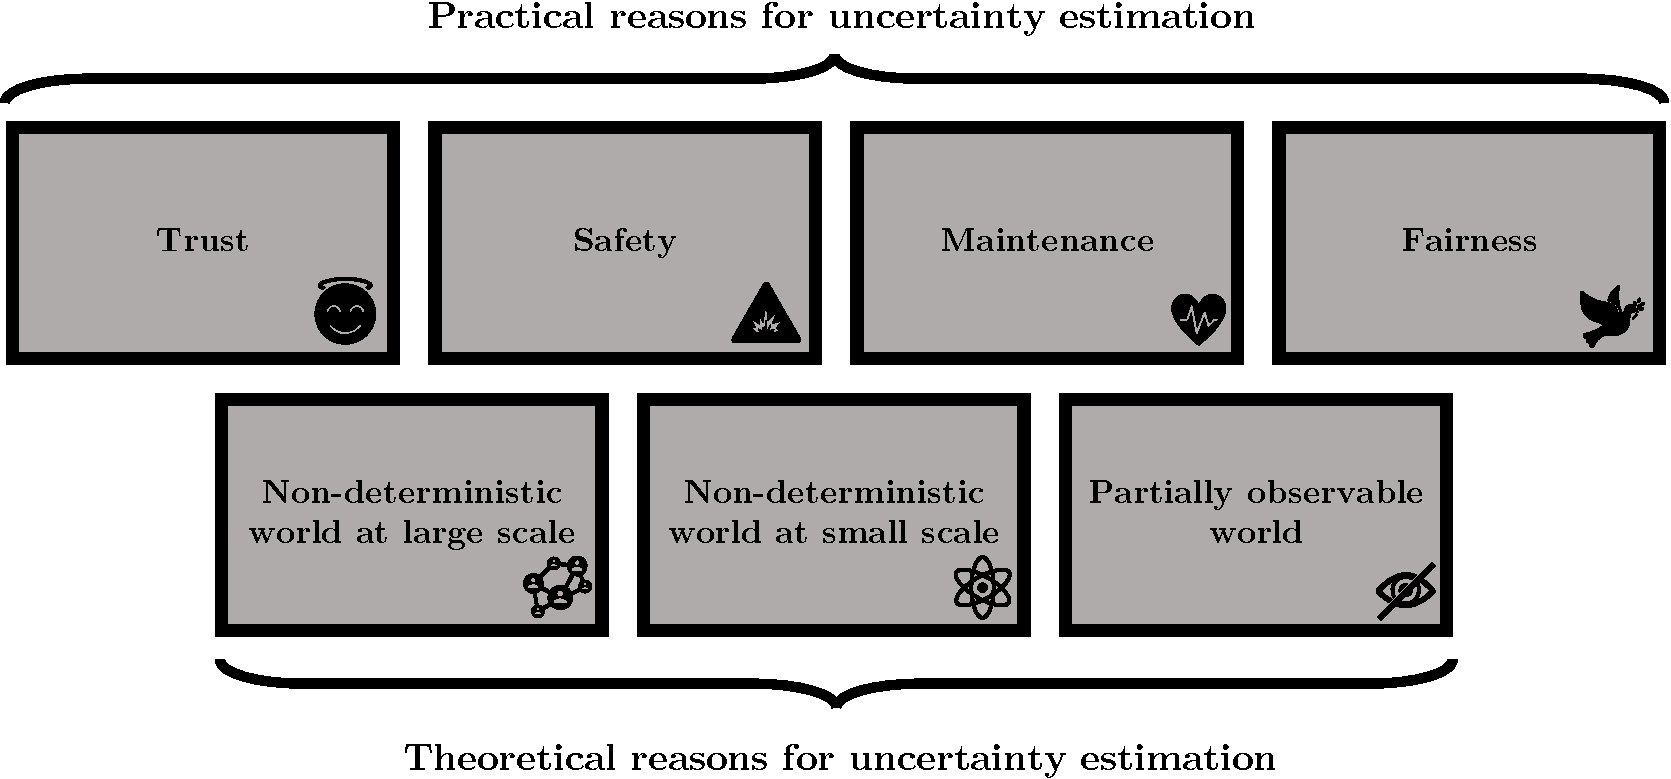
\includegraphics[width=0.9 \textwidth]{resources/uncertainty_reasons.pdf}}}$
    \end{subfigure}%
    \caption{Overview of the \emph{practical} and \emph{theoretical} reasons for uncertainty estimation.}
    \label{fig:uncertainty_reasons}
	% \vspace{-.5cm}
\end{figure}

\paragraph*{Practical reasons.} The Dunning-Kruger effect \cite{dunning-kruger} describes a psychological cognitive bias in which people lacking knowledge in a particular domain overestimate their abilities. Interestingly, this phenomenon also applies to machine learning models. Traditional neural networks show overconfident predictions, in particular on data that is different from the data seen during training \cite{overconfident-relu}. The illusion of knowledge of machine learning models highly impacts the reliability of such  models  in  safety-critical  domains.
First, it affects the \emph{trust} in ML model predictions. Ideally, we expect ML models to be confident when predicting correctly and uncertain when predicting wrongly. 
Second, it affects the \emph{safety} of ML predictions in unfamiliar situations. Ideally, we expect ML models to flag predictions on unknown domains corresponding to anomaly detection.
Third, it affects the \emph{maintenance} of ML models. Ideally, we expect ML models to become more uncertain when the testing data has drifted away from the training data, thus indicating the need of retraining the model. This is particularly important in application where ML models need to explore and learn all life-long.
Finally, it affects the \emph{fairness} of ML models. Ideally, we expect ML models to provide calibrated predictions on all input regions including underrepresented data.
A summary of the practical reasons and their associated use cases is given in table \bc{Do table}.

\paragraph*{Theoretical reasons.} ML models aim at precisely representing the flow of information in the world which is inherently uncertain.
The world is \emph{non-deterministic at a large scale}. Indeed, uncertainty emerges when small individual events contribute to macro phenomena like GDP growth, micro phenomena like the growth rate of firms, and non-economic events like war and climate change \cite{macro-micro-uncertainty}.
The world is \emph{non-deterministic at a small scale}. Indeed, the uncertainty principle in (quantum) physics implies that it is in general not possible to predict the value of a particle quantity (like position and speed) with arbitrary certainty, even if all initial conditions are specified \cite{hilgevoord2016heisenberg}.
The world is only \emph{partially observable}. Indeed, agents like humans or robots have to deal with incomplete information on the environment in which they evolve \cite{kaelbling1998pomdp}. At the extreme, since the speed of information is limited by the speed of light, accessible information is restricted to the observable world, thus making the world inherently uncertainty for any agent \cite{ord2021universe}.
A summary of the theoretical reasons is given in table \bc{table}.


\paragraph*{} All these reasons underline the need of accurate uncertainty estimation methods in ML. 
Specifically, a reliable ML model should provide high-quality estimates of \emph{aleatoric} and \emph{epistemic} uncertainty \citep{uncertainty-deep-learning}.
The aleatoric uncertainty allows a model to account for the irreducible data uncertainty (e.g. the inherent sensor noise, or the inherent environment stochasticity).
The epistemic uncertainty allows a model to account for its lack of knowledge about unseen data regions (e.g. testing data differs significantly from training data).
Aleatoric and epistemic uncertainty levels can eventually be combined into an overall \emph{predictive} uncertainty \citep{uncertainty-deep-learning}. Hence, this thesis studies the usage of different types of uncertainty for ML methods.

\section{Why do we need independent and non-independent data ?}

In this thesis, we consider ML models which process input data to accurately predict output targets. 
More specifically, we expect ML models to be able to process \emph{any type of input data} (e.g. tabular, images, graph or time series) to predict \emph{any type of output data} (e.g. classes, continuous values, counts).
To this end, \emph{independence} and \emph{non-independence} are key assumptions to create \emph{practical} and \emph{accurate} models which precisely describe the real-world. 

\begin{figure}[ht!]
    \centering
    \begin{subfigure}[t]{0.245 \columnwidth}
        \centering
        $\vcenter{\hbox{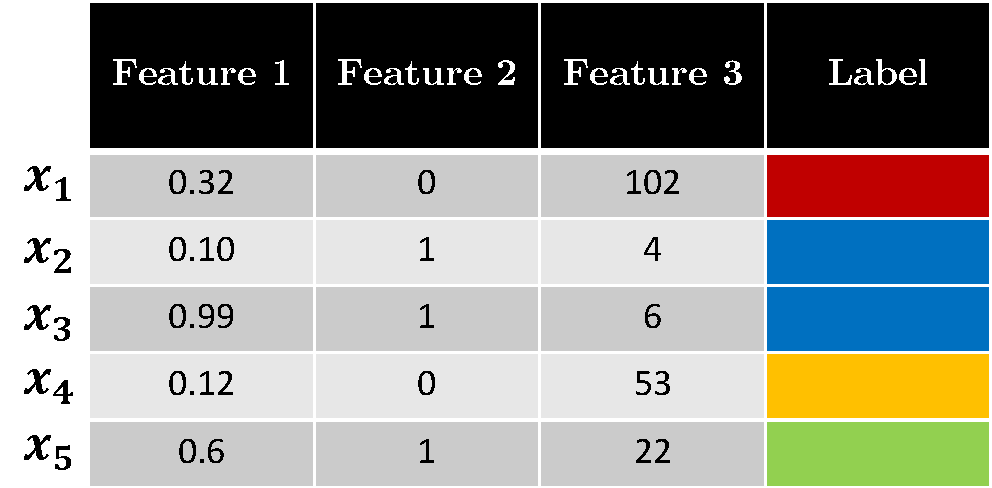
\includegraphics[width=0.9 \textwidth]{resources/tabular-cropped.pdf}}}$
         \caption{Tabular data}
         \label{fig:tabular_data}
    \end{subfigure}%
    \begin{subfigure}[t]{0.245\columnwidth}
        \centering
        $\vcenter{\hbox{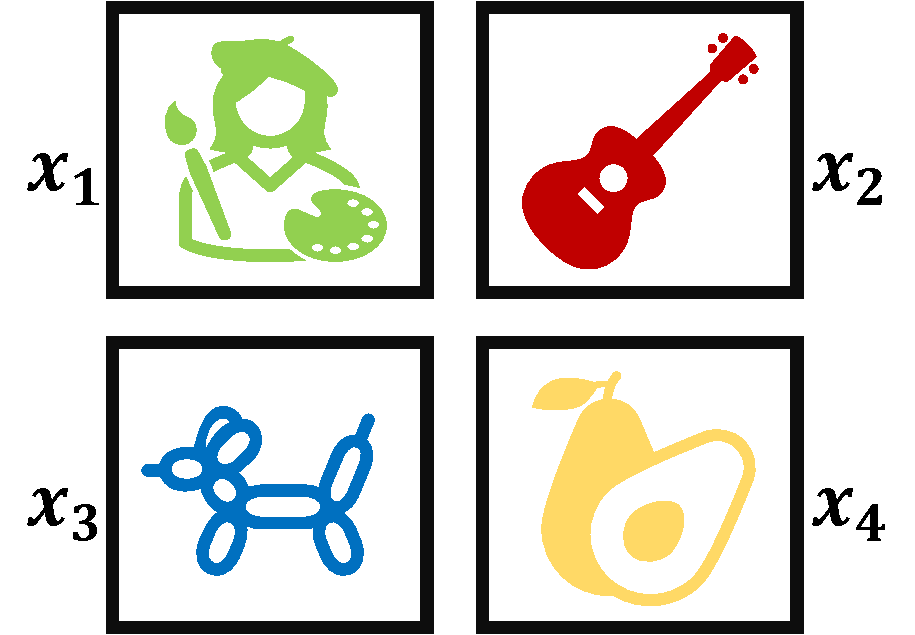
\includegraphics[width=0.9 \textwidth]{resources/image-cropped.pdf}}}$
        \caption{Image data}
        \label{fig:image_data}
    \end{subfigure}%
    \begin{subfigure}[t]{0.245 \columnwidth}
        \centering
        $\vcenter{\hbox{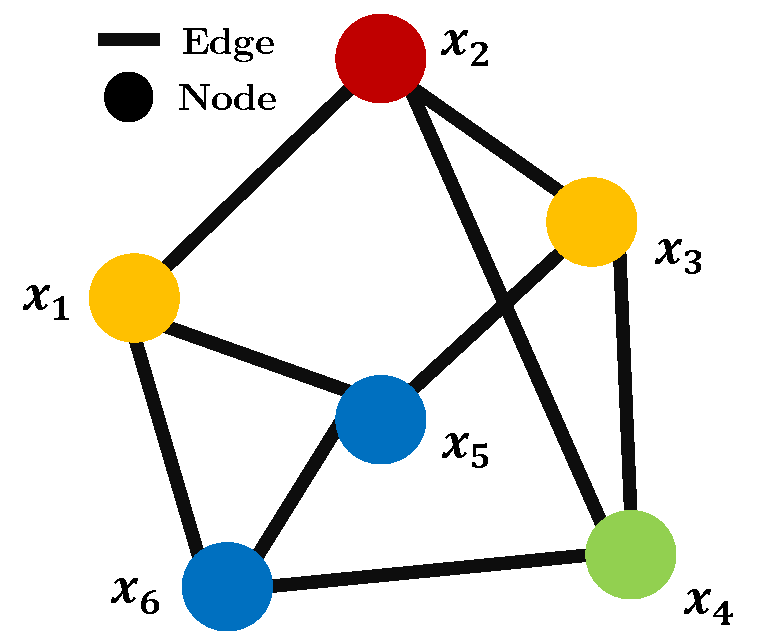
\includegraphics[width=0.9 \textwidth]{resources/graph-cropped.pdf}}}$
         \caption{Graph data}
         \label{fig:graph_data}
    \end{subfigure}%
    \begin{subfigure}[t]{0.245\columnwidth}
        \centering
        $\vcenter{\hbox{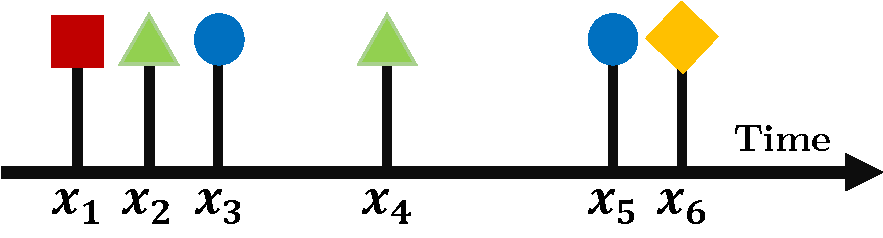
\includegraphics[width=0.9 \textwidth]{resources/sequential-cropped.pdf}}}$
        \caption{Sequential data}
        \label{fig:sequential_data}
    \end{subfigure}%
    \caption{Overview of different data types covering independent $\x_i$ inputs like tabular and image data, and dependent $\x_i$ inputs like graph node and sequential time events.}
	% \vspace{-.5cm}
\end{figure}

\paragraph*{Independent Data.} The independence assumption means that different data samples are not connected in any way. In other words, the knowledge of one data sample does not bring any information on another data sample.
The independence assumption is particularly useful when representing tabular data \cite{raschka2022chronology} (e.g. a group of unrelated persons for a medicine trial, defects on multiple different devices) or image data \cite{lu2020survey, litjens2017survey} (e.g. disease detection on medical images of different patients, object detection in different self-driving cars or robots). Visualizations of such data are represented in Fig.~\ref{fig:tabular_data} and Fig.~\ref{fig:image_data}.
In this case, representing the interaction between data samples does not bring much information to perform the predictions.
Hence, the key advantage of the independence assumption is that it allows mathematical factorization for practical modelling simplifications \citep{bishop} without important information loss.

\paragraph*{Non-Independent Data.} The non-independence assumption means that different data samples might be connected in some way. In other words, observing a data sample gives some information on the value of another data sample.
The non-independence assumption is particularly useful when representing graph data \cite{GNNBook2022} (e.g. social networks, citation networks) or sequential data \cite{shchur2021review, Dietterich2002Machine} (e.g. financial time series, interaction history of a user). Visualizations of such data are represented in Fig.~\ref{fig:graph_data} and Fig.~\ref{fig:sequential_data}.
In this case, neighboring nodes of a graph are expected to share important information and past events are expected to give important information on future events.
Hence, the key advantage of the non-independence assumption is that it retains the information contained in graph and sequential interactions to model the world more precisely.

\paragraph*{} Beyond the \emph{(non-)independence assumption}, another common assumption in ML is that data are \emph{identically distributed}. 
This assumption assumes that all input data comes from the same data distribution which also has strong limitations related to the reasons motivating the usage of uncertainty estimates for ML predictions.
While the training data are assumed to come from the same data distribution, the testing data might come from different distributions and suffer from \emph{Distribution Shifts} \cite{rabanser2019shift, dataset-shift}. 
Indeed, the testing data might come from the \emph{In-Distribution (ID)} similar to the training data, or a \emph{Out-Of-Distribution (OOD)} which could be any distribution different from the training distribution \cite{ood-detection-survey, shen2021ood}.
This scenario frequently happens in \emph{safety} and \emph{maintenance} use-cases where the data distribution observed by the model continuously drifts at testing time. 

Hence, this thesis acknowledges the limitation of the standard \emph{independent and identically distributed (i.i.d.)} assumptions.
To this end, this thesis studies the application of uncertainty estimation to independent and non-independent data.

\section{Contributions and outline}

This thesis studies the application of uncertainty estimation for independent and non-independent data via three main components:
\begin{itemize}
    \item Explicit \emph{desiderata} capturing the desired behavior of uncertainty estimation.
    \item Accurate \emph{models} for uncertainty estimation with low practical overhead.
    \item Practical \emph{experimental setup} evaluating uncertainty estimation in real-world applications including worst-case scenarios.
\end{itemize} 

To this end, we start by establishing the background knowledge about uncertainty estimation in Chapter~\ref{chap:background}.

In Part~\ref{part:independent_data}, we present a study of uncertainty estimation for \emph{independent data}: 
In Chapter~\ref{chap:classification}, we construct a new Bayesian model for uncertainty estimation for classification called \PostNet{} (\PostNetacro{}). \PostNetacro{} requires a \emph{single-forward pass}, does need \emph{no OOD data during training}, and adapt to \emph{many core architectures}.
In Chapter~\ref{chap:regression}, we construct a new Bayesian model for uncertainty estimation for regression called \NatPN{} (\NatPNacro{}). Beyond regression, \NatPNacro{} applies to a \emph{large variety of supervised tasks} (incl. classification and count prediction) with \emph{very low computational overhead}.
In Chapter~\ref{chap:robustness}, we present the first study of the robustness of uncertainty models in the worst-case scenario of adversarial attacks. We show that uncertainty estimates of an important family of single-forward pass models are \emph{not robust} for many important real-world tasks (incl. correct/wrong prediction detection, adversarial examples detection, and ID/OOD detection). Further, we explore first approaches methods to improve uncertainty robustness by using \emph{adversarial training} and \emph{randomized smoothing}. 

In Part~\ref{part:non_independent_data}, we present a study of uncertainty estimation for \emph{non-independent data}:
In Chapter~\ref{chap:graph_data}, we present the first framework for uncertainty estimation for node classification on graph data. This framework proposes explicit desiderata, a new Bayesian model, and an exhaustive evaluation setup which cover aleatoric and epistemic uncertainty estimation \emph{without} and \emph{with network effects}.
In Chapter~\ref{chap:sequential_data}, we present new models for uncertainty estimation in sequential data with asynchronous time events. The two proposed models are able of accurate \emph{event types} and \emph{event time} predictions while capturing \emph{uncertainty with rich temporal evolution}.
In Chapter~\ref{chap:reinforcement_learning}, we present the first framework to disentangle aleatoric and epistemic uncertainty estimation in reinforcement learning. This framework proposes explicit desiderata, four models inspired from supervised learning, and a detailed experimental setup which cover aleatoric and epistemic uncertainty estimation at both \emph{training time} and \emph{testing time}.

In Part~\ref{part:conclusion}, we present a retrospective on the evolution of the research field since our first study (see Chapter~\ref{chap:retrospective}) and a conclusion including open questions as suggestion to future research directions (see Chapter~\ref{chap:conclusion}).

\begin{table}
    \caption{List of own publications that this thesis is based on. Code and datasets for the respective publications are available at \texttt{www.cs.cit.tum.de/daml/[project]}.}
    \vspace{2mm}
    \label{tab:publications}
    \begin{adjustbox}{max width=\textwidth}
    \begin{tabular}{lllll}
      {Ch.} & {Ref.} & {Title} & {Conference} & {Repository}\\
      \midrule
      \ref{chap:classification} & \cite{charpentier2020} & \makecell[l]{Posterior network: Uncertainty estimation without\\ ood samples via density-based pseudo-counts} & NeurIPS 2020 & \texttt{/postnet/}\\
      \ref{chap:regression} & \cite{NatPN2021} & \makecell[l]{Natural posterior network: Deep bayesian predictive\\ uncertainty for exponential family distributions.} & ICLR 2021 & \texttt{/natpn/}\\
      \ref{chap:robustness} & \cite{robustness-uncertainty-dirichlet} & \makecell[l]{Evaluating robustness of predictive uncertainty estimation:\\ Are dirichlet-based models reliable?} & ICML 2020 & \texttt{/dbu-robustness/}\\
      \ref{chap:graph_data} & \cite{graph-postnet} & \makecell[l]{Graph posterior network: Bayesian predictive uncertainty\\ for node classification.} & NeurIPS 2021 & \texttt{/graph-postnet/}\\
      \ref{chap:sequential_data} & \cite{uceloss} & \makecell[l]{Uncertainty on asynchronous time event prediction} & NeurIPS 2019 & \texttt{/uncertainty-event-prediction/}\\
      \ref{chap:reinforcement_learning} & \cite{charpentier2022uncertainty-rl} & \makecell[l]{Disentangling epistemic and aleatoric uncertainty\\ in reinforcement learning} & DFUQ - ICML 2022 & \texttt{/aleatoric-epistemic-uncertainty-rl/}\\
    \end{tabular}
    \end{adjustbox}
\end{table}

\section{Own publications}

The content of Chapters \ref{chap:classification} to \ref{chap:reinforcement_learning} is mostly based on papers previously published at international peer-reviewed conferences. We list these papers in Table~\ref{tab:publications}.
We also provide the full list of publications that the author was involved in during the PhD studies below. These publications focus on three main topics: \emph{uncertainty estimation} (incl. bayesian models, energy-based models and robustness), \emph{structure learning} (incl. hierarchical and directed acyclic graphs), and \emph{efficient ML} (incl. pruning methods and sparse neural networks).

\renewcommand{\bibsection}{}
\documentclass{article}
\usepackage[numbers]{natbib}
\begin{document}
\nocite{charpentier2020}
\nocite{NatPN2021}
\nocite{robustness-uncertainty-dirichlet}
\nocite{graph-postnet}
\nocite{uceloss}
\nocite{ood_ebm}
\nocite{charpentier2019tsd}
\nocite{bonald2020scikitnetwork}
\nocite{zugner2022endtoend}
\nocite{rachwan2022earlycrop}
\nocite{ayle2022robustness-sparse}
\nocite{charpentier2022uncertainty-rl}
\nocite{charpentier2022dpdag}
\nocite{charpentier2023training}
\nocite{getzner2023accuracy}

\bibliographystyle{plain}
\bibliography{../../bibliography}
\end{document}
\chapter{Background}
\label{chap:background}

\epigraph{Science is the outcome of being prepared to live without certainty and therefore a mark of maturity. It embraces doubt and loose ends.}{\textit{A.C. Grayling}}

In this chapter, we introduce the main background on the content of this thesis. It covers background on the desiderata, models, and metrics for uncertainty estimation in Machine Learning. In order to preserve the original storyline of the original publications, we kept the background sections in \cref{chap:classification,chap:regression,chap:robustness,chap:graph_data,chap:sequential_data,chap:reinforcement_learning}. Beyond this chapter, we also recommend existing surveys on uncertainty estimation for further details on uncertainty estimation in deep learning \citep{uncertainty-survey,review-uncertainty-dl,psaros2023uncertainty,conformal-survey,hullermeier2021aleatoric}.

\section{Uncertainty desiderata}
\label{sec:background-desiderata}

In this section, we review important desiderata for uncertainty estimation. We provide a summary of these desiderata in \cref{tab:overview_desiderata}.

\begin{table*}[ht]
    \begin{center}
    \resizebox{1.\textwidth}{!}{%
    \begin{tabular}{c}
    \toprule
    \textbf{Bayesian distributions} \\
    \midrule
    \midrule
    $\prior(\bm{\phi} \condition \data)$ where $\bm{\phi}$ are model weights \\
    $\prior(\bm{a} \condition \data, \x)$ where $\bm{a}$ are values of the activations \\
    $\prior(\bm{\theta} \condition \data, \x)$ where $\bm{\theta}$ are parameters of the target distribution \\
    \bottomrule
    \end{tabular}%
    \quad
    \begin{tabular}{c}
        \toprule
        \textbf{Uncertainty types} \\
        \midrule
        \midrule
        Aleatoric uncertainty \\
        Epistemic uncertainty \\
        Predictive uncertainty \\
        \bottomrule
    \end{tabular}%
    \quad
    \begin{tabular}{c}
        \toprule
        \textbf{Practical requirements} \\
        \midrule
        \midrule
        Efficiency: Data \& Time \\
        Flexibility: Architecture \& Optimization \\
        Robustness: Natural \& Adversarial \\
        \bottomrule
    \end{tabular}%
    }
    \end{center}
    \caption{Overview of desiderata for models for uncertainty estimation. Important desiderata involve modelling Bayesian distributions, distinguishing between uncertainty types, and fulfilling practical requirements.}
    \label{tab:overview_desiderata}
\end{table*}

% \begin{table*}[ht]
%     \begin{center}
%     \resizebox{1.\textwidth}{!}{%
%     \begin{tabular}{ccc}
%     \toprule
%     \textbf{Bayesian distributions} & \textbf{Uncertainty types} & \textbf{Practical requirements} \\
%     \midrule
%     \midrule
%     $\prior(\bm{\phi} \condition \data)$ where $\bm{\phi}$ are model weights &  Aleatoric uncertainty & Efficiency: Data \& Time \\
%     $\prior(\bm{a} \condition \data, \x)$ where $\bm{a}$ are values of the activations &  Epistemic uncertainty & Flexibility: Architecture \& Optimization \\
%     $\prior(\bm{\theta} \condition \data, \x)$ where $\bm{\theta}$ are parameters of the target distribution &  Predictive uncertainty & Robustness: Natural \& Adversarial \\
%     \bottomrule
%     \end{tabular}%
%     }
%     \end{center}
%     \caption{Overview of desiderata for models for uncertainty estimation. Important desiderata involve modelling Bayesian distributions, distinguishing between uncertainty types, and fulfilling practical requirements.}
%     \label{tab:overview_desiderata}
% \end{table*}

\subsection{Bayesian Distributions} 

Bayesian distributions offer a convenient framework to express beliefs in the realization of an event. In particular, the Bayesian framework allows to easily incorporate prior knowledge and update our beliefs given additional new observations in a principled way. Hence, we first recall the key concept of the Bayesian framework since it is a core concept in many uncertainty estimation approaches.

\paragraph{Unsupervised learning.} We define the distribution $\prob(\y \condition \bm{\theta})$ over the target variable $\y \in \real^K$ given the parameter $\bm{\theta}$.
Given a dataset $\data=\{\y^{(1)}, ..., \y^{(\ndata)}\}$, the Bayes formula is:
\begin{equation}
    \prior(\bm{\theta} \condition \data) = \frac{\prob(\data \condition \bm{\theta}) \times \prior(\bm{\theta})}{\prob(\data)}
\end{equation}
where $\prob(\data \condition \bm{\theta})$ is the \emph{likelihood}, $\prior(\bm{\theta})$ is the \emph{prior}, $\prior(\bm{\theta} \condition \data)$ is the \emph{posterior}, and $\prob(\data)$ is the \emph{evidence}.
Intuitively, the Bayesian formula updates the prior belief represented by $\prior(\bm{\theta})$ into the posterior belief represented by $\prior(\bm{\theta} \condition \data)$ after observing a dataset $\data$ \cite{bishop}.
The choice of prior is crucial. A common choice is to follow the \emph{principle of maximum entropy} \citep{maximum-entropy-principle} and enforce high entropy for the prior distribution which is usually considered less informative. However, note that many works studied different choices of priors \cite{jeffreys1946prior, silvestro2020prior}.
The evidence term $\prob(\data)$ corresponds to a normalization constant which can sometimes be ignored \cite{bishop}.

After observing a dataset $\data$, we can update the distribution over the target variable $\y$ in two ways.
A first option is to use a point-wise estimate of the target distribution parameter, i.e.:
\begin{equation}
    \prob(\y \condition \bm{\theta}^*)
\end{equation}
where $\bm{\theta}^*=\argmax\prior(\y \condition \bm{\theta})$ would be the maximum likelihood estimate, or $\bm{\theta}^*=\argmax\prior(\bm{\theta} \condition \data)$ would be the maximum a posteriori estimate.
A second option is to integrate over all possible values for the target distribution parameter, i.e.:
\begin{equation}
    \label{eq:posterior_predictive}
    \prob(\y \condition \data) = \int \prob(\y \condition \bm{\theta}) \prior(\bm{\theta} \condition \data) d\bm{\theta}
\end{equation}
where $\prob(\y \condition \data)$ is called the posterior predictive distribution. 
This second approach is often considered to be more Bayesian since it depends on the full posterior distribution $\prior(\bm{\theta} \condition \data)$.
However, it might be costly to compute the posterior distribution since it requires integration.

\paragraph{Supervised learning.} In supervised learning, the goal is to predict the value of a target output variable $\y$ given an input $\x$ after observing a dataset $\data=\{(\x^{(1)}, \y^{(1)}), ...,$ $(\x^{(\ndata)}, \y^{(\ndata)})\}$.
In this case the posterior predictive requires to be adapted with three main options: compute the posterior distribution over the weights $\prior(\bm{\phi} \condition \data)$, compute the posterior over the activations $\prior(\bm{a} \condition \data, \x)$, and compute the posterior over the parameters of the target distribution $\prior(\bm{\theta} \condition \data, \x)$ (see \cref{tab:overview_desiderata} left). The first option is:
\begin{equation}
    \label{eq:factorization_1}
    \prob(\y \condition \data, \x) = \int \prob(\y \condition \bm{\phi}, \x) \prior(\bm{\phi} \condition \data) d\bm{\phi}
\end{equation}
where $\bm{\phi}$ denote the model weights. In this case, the parameter distribution $\prior(\bm{\phi} \condition \data)$ is not conditioned on the input $\x$ and only accounts for an uncertainty dependent on the dataset $\data$. Examples of such models are Bayesian neural networks which learn Bayesian distribution $\prior(\bm{\phi} \condition \data)$ where $\bm{\phi}$ denote the model weights \cite{bayesian-networks}.
The second option is:
\begin{equation}
    \label{eq:factorization_2}
    \prob(\y \condition \data, \x) = \int \prob(\y \condition \bm{a}) \prior(\bm{a} \condition \data, \x) d\bm{a}
\end{equation}
where $\bm{a}$ denote intermediate representations of $\x$. In this case, the parameter distribution $\prior(\bm{a} \condition \data, \x)$ is conditioned on the new input $\x$ and accounts for an uncertainty dependent on the input $\x$. Examples of such models are Bayesian neural networks which learn Bayesian distribution $\prior(\bm{a} \condition \data, \x)$ where $\bm{a}$ denote the values of the activations \cite{gp-uncertainty-activation,natural-parameter-network}.
Alternatively, the third option is:
\begin{equation}
    \label{eq:factorization_3}
    \prob(\y \condition \data, \x) = \int \prob(\y \condition \bm{\theta}) \prior(\bm{\theta} \condition \data, \x) d\bm{\theta}
\end{equation}
where $\bm{\theta}$ denote the direct parameters of the distribution over the target $\y$. In this case, the parameter distribution $\prior(\bm{\theta} \condition \data, \x)$ is conditioned on the new input $\x$ and also accounts for an uncertainty dependent on the input $\x$. Examples of such models are the Bayesian neural networks proposed in this thesis \cite{charpentier2020,natpn, graph-postnet,charpentier2022uncertainty-rl,uceloss} which learn Bayesian distributions $\prior(\bm{\theta} \condition \data, \x)$ where $\bm{\theta}$ denote the parameters of the distribution over the target labels $\y$. In this thesis, we focus on learning  Bayesian distributions on the (generally) low dimensional target parameters $\bm{\theta}$, in contrast to the (generally) high dimensional activation $\bm{a}$ or weights  $\bm{\phi}$, thus advantageously allowing to reduce the computation complexity of the posterior distribution.

\subsection{Aleatoric, Epistemic \& Predictive Uncertainty}

The Bayesian formula in \cref{eq:posterior_predictive} involves three types of distribution (i.e. $\prob(\y \condition \bm{\theta})$, $\prior(\bm{\theta} \condition \data)$, and $\prob(\y \condition \data)$) which cover the three main sources of uncertainty: the aleatoric uncertainty represented by the distribution $\prob(\y \condition \bm{\theta})$, the epistemic uncertainty represented by the distribution $\prior(\bm{\theta} \condition \data)$, and the predictive uncertainty represented by the distribution $\prob(\y \condition \data)$ (see \cref{tab:overview_desiderata} middle).

\textbf{Aleatoric uncertainty.} The \emph{aleatoric uncertainty} is sometimes also called data uncertainty, stochastic uncertainty or risk \cite{hullermeier2021aleatoric,knight1921, malini2018}. 
The aleatoric uncertainty is represented by the distribution $\prob(\y \condition \bm{\theta})$.
The aleatoric uncertainty should be high when \emph{the model does not know because of inherent noise in a given context} (e.g. noisy environment, noisy sensors, low computation resources, model mispecification) \cite{wenger2022posterior, hullermeier2021aleatoric}.
Given a specific context, the aleatoric uncertainty is \emph{irreducible} since additional observations cannot resolve the information loss due noisy measurements or misspecifications. 
However, aleatoric uncertainty can be reduced by using higher measurement resolution or improving the model specification. 

\textbf{Epistemic uncertainty.} The \emph{epistemic uncertainty} is sometimes also called knowledge uncertainty, systematic uncertainty, or knightian uncertainty \cite{hullermeier2021aleatoric,knight1921,malini2018}.
The epistemic uncertainty is represented by the distribution $\prior(\bm{\theta} \condition \data)$.
The epistemic uncertainty should be high when \emph{the model does not know because of a lack of observed data} in the dataset $\data$.
Hence, the epistemic uncertainty is \emph{reducible} since it should decrease when collecting additional data.

\textbf{Predictive uncertainty.} The \emph{predictive uncertainty} is sometimes also called total uncertainty \cite{hullermeier2021aleatoric,malini2018}.
The predictive uncertainty is represented by the distribution $\prob(\y \condition \data)$.
Intuitively, the predictive uncertainty aggregates the effect of the aleatoric and epistemic uncertainty by integrating jointly the distributions $\prob(\y \condition \bm{\theta})$ and $\prior(\bm{\theta} \condition \data)$.

In practice, each uncertainty type can be measured by computing the spread of its respective distribution with the (differential) entropy which represents its variability \citep{PriorNetworks,uncertainty-deep-learning}, i.e.:
\begin{align}
     u_\text{alea} = \entropy[\prob(\y \condition \bm{\theta})], \hspace{4mm}
     u_\text{epist} = \entropy[\prior(\bm{\theta} \condition \data)], \hspace{4mm}
     u_\text{pred} = \entropy[\prob(\y \condition \data)]
\end{align}
Apart from the entropy, other uncertainty metrics can be commonly used. E.g. the variance of the distributions can indicate different uncertainty types, the max probability for classification \cite{malini2018} can indicate the aleatoric uncertainty, or the concentration parameters can indicate the epistemic uncertainty if they exist \cite{charpentier2020}.

In this thesis, we focus on methods capable to estimates the three types of uncertainty types.

\subsection{Efficiency, Flexibility \& Robustness}

Uncertainty methods are also expected to have practical characteristics (see \cref{tab:overview_desiderata} right). 

First, an uncertainty method is expected to be \emph{efficient} at both training and testing time. 
A first aspect is \emph{time efficiency} meaning that the method should be fast with low computational overhead. E.g. uncertainty methods requiring multiple forward passes are usually more expensive than method require a single forward pass.
As second aspect is \emph{data efficiency} meaning that the method should require as few data as possible to train.

Second, an uncertainty method is expected to be \emph{flexible}.
A first aspect is \emph{architecture flexibility} meaning that the method should easily adapt to any architectures in order to easily adapt to different input types (e.g. tabular, images, graphs, and sequential data) and output types (e.g. classification and regression).
A second aspect is \emph{optimization flexibility} meaning that the method should easily adapt to different training schemes including end-to-end training or fine-tuning based on pretrained models.

Finally, an uncertainty method is expected to be \emph{robust}.
A first aspect is \emph{natural robustness} meaning that the method should be performant even if there is some natural drift in the data. Natural drifts could be due to time evolution or location variability \cite{wilds, neuhold201mapillary, shifts-dataset}.
A second aspect is \emph{adversarial robustness} meaning that the method should be performant even against adversarial perturbations which are specifically designed to fool the model. Adversarial perturbations can be viewed as the worst-case scenario for the model. Different methods to compute adversarial perturbations including white box attacks which do not have information about the model, black box attacks which have full access to the model information, and gray box which have partial information about the model \cite{han2020adversarial}.

In this thesis, we focus on proposing practical methods which are efficient in terms of data and time, flexible in terms of architecture and optimization schemes, and robust in terms of natural and adversarial perturbations.

\section{Uncertainty models}
\label{sec:background-models}

In this section, we review important families of models for uncertainty estimation. We provide a summary of these models in \cref{fig:overview_methods}. We refer the reader to seed papers and surveys provided in the following paragraphs presenting each family of methods for a detailed presentation of their concepts. Overall, we observed that these families of methods could be approximately be classified in two groups. On one hand, ensembles, Monte Carlo dropout, Markov chain Monte Carlo, variational inference, Laplace approximation, and Gaussian process methods form a first group of methods with strong Bayesian guarantees but often requiring expensive computations. On the other hand, evidential, calibration, density-based, energy-based, and distance-based methods form a second group of methods sometimes capable of efficient uncertainty predictions to the cost of weaker Bayesian guarantees or additional practical constraints like the need of additional training or validation data.

\begin{figure}[ht!]
    \centering
    \begin{subfigure}[t]{1. \columnwidth}
        \centering
        $\vcenter{\hbox{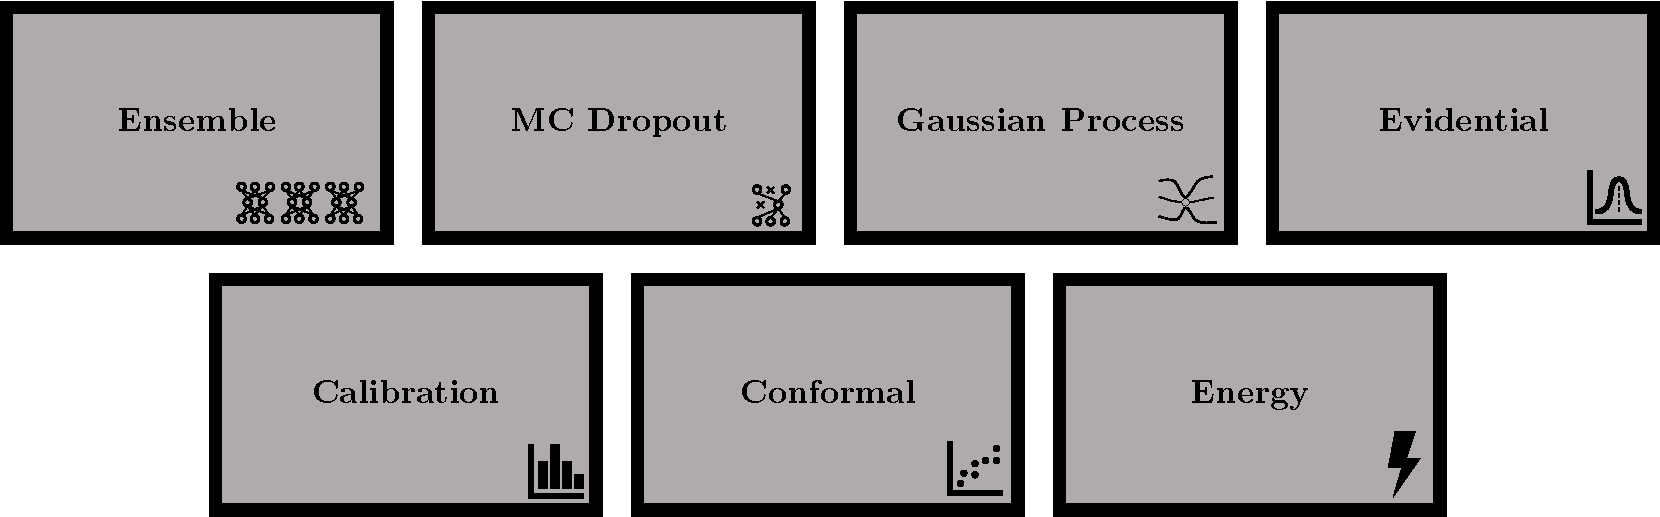
\includegraphics[width=0.9 \textwidth]{resources/overview_methods.pdf}}}$
    \end{subfigure}%
    \caption{Overview of the different families of methods for uncertainty estimation.}
    \label{fig:overview_methods}
	% \vspace{-.5cm}
\end{figure}

% Add a table with useful existing implementations/packages of those methods

\paragraph*{Ensembles.} This family of methods consists in combining the predictions of a set of multiple models $f_{\bm{\phi}_1},\cdot, f_{\bm{\phi}_K}$ by using stacking, bagging, boosting, Bayesian averaging or other Bayesian combinations \citep{bayesian-averaging-to-combination}. The variance of the different model predictions can be viewed as uncertainty estimates. These uncertainty estimates can be considered Bayesian where the member weights are sampled from the posterior weight distribution, i.e. $\bm{\phi}_k \sim \prior(\bm{\phi} \condition \data)$. The ensembles can be \emph{homogeneous ensembles}, i.e. the models share the same architecture, be \emph{heterogeneous ensembles}, i.e. the models have different architectures, or \emph{implicit ensembles}, i.e. a single model approximated ensembles parameter sampling \citep{abe2022deep}. Further, the different models can be trained sequentially (see e.g. \citep{schapire2013explaining, chenG16xgboost}) or independently (see e.g. \citep{ensembles}).
%
Ensembles are considered as strong baselines in terms of uncertainty estimation and predictive performances \citep{dataset-shift}. Ensembles also benefit from a simple implementation \citep{ensembles}.
%
Ensembles are often considered to be expensive as they require multiple forward passes. Many approaches \citep{batch-ensembles,mimo-independent-subnetworks} proposed to make faster ensembles. Further, while ensembles improve predictive performance, this performance gain can actually be replicated through the use of (larger) single models \citep{abe2022deep}.

\paragraph*{Variational Inference.} This family of methods consists in approximating a (generally intractable) posterior distribution with a variational distribution belonging to a tractable family of distributions \cite{blei2017vi}. The approximate posterior distribution is often optimized using an Evidence Lower Bound (ELBO) loss. Many methods (see e.g. \cite{practical-bnn,bayesian-networks,practical_deep_bayesian_principles}) are interested in the posterior distribution over the model weights, i.e. $\prior(\bm{\phi} \condition \data)$ where $\bm{\phi}$ are the model weights. Thus, similarly to ensembles, uncertainty estimates can be obtained by sampling from the posterior distribution on the weights and computing the variance of their predictions. These methods generally needs to trade off the expressivity of the posterior distribution with computational complexity. To approximate the posterior distribution over the high dimensional weights, many works proposed to use techniques like mean-field approximations \citep{practical-bnn,bayesian-networks,practical_deep_bayesian_principles}, normalizing flows \cite{radialflow,Louizos2017}, or matrix decomposition with low rank or Kronecker products \cite{mishkin2018slang,bae2018eigen,zhang2017noisy}. In contrast with methods which are interested in posterior distributions $\prior(\bm{\phi} \condition \data)$ over model weights $\bm{\phi}$, we present in this thesis variational methods which approximate the posterior distribution $\prior(\bm{\theta} \condition \data, \x)$ over the target distribution parameters $\bm{\theta}$ (see \cref{chap:classification,chap:regression}).

\paragraph*{Monte Carlo Dropout.} Monte Carlo (MC) dropout consists in randomly dropping neurons to form different models $f_{\bm{\phi}_1},\cdot, f_{\bm{\phi}_K}$ and combine their predictions \citep{dropout} at both training and testing time. This approach can be considered as an ensemble of implicit models \citep{abe2022deep} but also as performing variational inference \citep{dropout}. Hence, similarly to ensembles, the variance of the predictions can be viewed as Bayesian uncertainty estimates the member weights are sampled from the posterior weight distribution, i.e. $\bm{\phi}_k \sim \prior(\bm{\phi} \condition \data)$. Many works extended this approach for e.g. convolutional layers \citep{tassi2020bayesian} or dropping connection instead of activations \citep{wan2013dropconnect}.

\paragraph*{Markov Chain Monte Carlo.} Markov Chain Monte Carlo (MCMC) methods, consists in building a Markov Chain which will converge to samples from the posterior distribution. A key example is the Metropolis-Hastings algorithm which iteratively draw a sample from a transition rule and then decide to accept or reject it \cite{robert2015metropolis}. Many works focus on sampling from the approximate posterior distribution $\prior(\bm{\phi} \condition \data)$ over model weights $\bm{\phi}$ (see e.g. \citep{duane1987hybrid,welling2011langevin}). In this case, the Markov Chain builds a sequence $\bm{\phi},\cdot,\bm{\phi}_t$ by following e.g. Hamiltonian dynamics \citep{duane1987hybrid} or Stochastic Gradient Langevin Dynamics \cite{welling2011langevin,garriga-alonso2021exact,ma2015mcmc} which converge to sample from the posterior distribution, i.e. $\bm{\phi}_t \sim \prior(\bm{\phi} \condition \data)$ when $t \rightarrow \infty$. On one hand, while full batch MCMC has managed to scale to modern tasks and models, they often come at a heavy computational cost \citep{what-bnn-posterior}. On the other hand, while stochastic gradient MCMC improve the computational efficiency \cite{welling2011langevin,garriga-alonso2021exact,ma2015mcmc}, it might introduce bias in the stationary distribution by omitting the Metropolis-Hasting rejection or subsampling the data \citep{betancourt2015data,what-bnn-posterior}.

\paragraph*{Laplace Approximation.} The Laplace approximation consists in approximating the posterior distribution with a Gaussian distribution centered around a mode of the posterior distribution. Many works focus on approximating the posterior distribution $\prior(\bm{\phi} \condition \data)$ over model weights $\bm{\phi}$. In this case the Laplace approximation gives:
\begin{align*}
    \prior(\bm{\phi} \condition \data) \approx \DNormal(\bm{\phi}_\text{MAP}, \bm{\Sigma})
\end{align*}
where $\bm{\phi}_\text{MAP}$ is the maximum a posteriori estimate, and $\bm{\Sigma}=-(\nabla_{\bm{\phi}}^2 \left.\loss(\data;\bm{\phi})\right|_{\bm{\phi}_\text{MAP}})^{-1}$ is the Laplace approximation of the covariance based on the Hessian of the loss. The posterior distribution can be defined on all model weights, subnetworks \cite{daxberger2021bayesian}, or only the last layer \cite{bayesian-a-bit}. The Hessian computation can be costly and can be approximated using the different techniques like the Fisher information matrix, the generalized Gauss-Newton matrix, diagonal factorization, Kronecker-factored approximate curvature, or low-rank approximation \citep{daxberger2021laplace}. Finally, the computation of the predictive distribution needs further approximation like linearizing the neural network or using Monte-Carlo approximation \citep{daxberger2021laplace}.

\paragraph*{Gaussian Process.} Gaussian Processes (GPs) are a family of Bayesian methods which, given a dataset $\data$, associates to each new input $\x$ a predictive Gaussian distribution over the output $\y \sim \prob(\y \condition \data, \x) = \DNormal(m(\x), \sigma^2(\x))$. The mean function $m(\x)$ and the variance function $\sigma^2(\x)$ depends on the kernel function $\kappa(.,.)$ which encodes the similarity between data samples. Intuitively, uncertainty estimates can be obtained by computing the variance or the entropy of the predicted Gaussian distribution.
On one hand, standard GPs have computational and storage limitations \cite{jakkala2021deepgp}. E.g. the computation of the variance function is cubic in the number of data samples which does not scale well to large datasets. To mitigate this issue, previous works proposed sparse Gaussian process which introduce variational pseudo-points can be optimized with stochastic gradient descent (see e.g. \cite{snelson2005sparse,titsias2010gplvm,due}).
On the other hand, standard GPs does not naturally extract hierarchical representations from structured data. To mitigate this issue, previous works proposed e.g. to use multilayer GPs \cite{damianou2012deepgp} or deep neural networks as the kernel function \cite{wilson2016stochastic}. We refer to existing survey on Gaussian process in deep learning for further details \citep{gp-for-ml,damianou2012deepgp,jakkala2021deepgp}.

\paragraph*{Evidential.} Evidential methods are derived from the theory of evidence which can be seen as generalization of the Bayesian theory to subjective probables \cite{dempster1968evidence,shafer1976mathematical}. Instead of predicting directly the parameters $\bm{\theta}$ of the target distribution $\prob(\y \condition \bm{\theta})$, evidential methods consist in predicting the parameters of the distribution $\prior(\bm{\theta} \condition \data, \x)$ defined over the parameters $\bm{\theta}$, thus following the factorization in \cref{eq:factorization_3}. In this case, uncertainty estimates can be obtained by computing the variance or the entropy of the predicted target or evidential distributions. This family of models is generally effective since it only requires a single forward pass for uncertainty estimation. To improve performances of evidential models, other works proposed to use OOD data during training \cite{PriorNetworks,reverse-kl}, knowledge distillation \cite{distribution-distillation}, or contrastive learning \cite{uncertainty-generative-classifier}. In this thesis, we introduce a new family of evidential models called \emph{Posterior networks} with a clear Bayesian interpretation and low practical overhead (see \cref{chap:classification,chap:regression,chap:robustness,chap:graph_data,chap:sequential_data,chap:reinforcement_learning}). We refer to existing survey on evidential deep learning for uncertainty quantification for further details \citep{survey_evidential_uncertainty}.

\paragraph*{Calibration.} Calibration metrics consists at evaluating if the probabilities predicted by a model correspond to the true probabilities of the model to be correct (see \cref{sec:calibration} for further details). Hence, in order to achieve high performance w.r.t. calibration metrics, calibration methods aim at predicting probabilities which are good approximations of their true probability of correctness. Beyond uncertainty-aware models which are expected to be well-calibrated, we distinguish between two other groups of calibration methods: during-training calibration methods and post-training calibration methods. During-training calibration methods apply regularization techniques in the loss objective to create inherently calibrated models (see e.g. \cite{lee2018training,corbieres2019confidence,minderer2021revisiting}). Post-training calibration methods recalibrate the model predictions after training (see e.g. \cite{calibration-network,wenger201calibration}). While these methods can adapt well to different architectures types, they usually require additional held-out validation data and assume that validation and test distribution are similar. Prominent classes of post-training calibration method are histogram binning \cite{zadrozny2001calibrated}, Temperature scaling \cite{calibration-network}, isotonic calibration \cite{zadrozny2002transforming}, Dirichlet calibration \cite{kull2019beyond}, or conformal predictions \cite{conformal-survey,marx2022conformal}.

\paragraph*{Density-based models.} This family of models assigned to every data sample $\x$ a probability density estimate $\prob(\x \condition \bm{\phi})$. In this case, a data sample considered uncertain by the model should be assigned a low density value while a data sample considered certain for the model should be assigned a high density value. The density estimator can be of different nature like a mixture of Gaussian \cite{simple_ood_adv_detection,du2022vos} or a normalizing flow \cite{nf-review,why-nf-fail-ood,postels2020hiddenuncertainty}. The choice of space on which the density estimator operates is crucial. While density estimation on the input space might be difficult due to the curse of dimensionality \citep{anomaly-detection,deep-generative,typicality_OOD_generative}, other works \cite{charpentier2020, why-nf-fail-ood, density-states-ood, contrastive-ood} improved the performance of density-based methods on uncertainty tasks by leveraging a task-induced bias or low-dimensional statistics. In particular, density-based models methods have achieved impressive success in OOD detection tasks \cite{ood-detection-survey}.

\paragraph*{Energy-based models.} Energy-based models (EBMs) associate to every combination of input $\x$ and output $\y$, a scalar energy value $E_{\bm{\phi}}(\y, \x)$ \cite{lecun2006tutorial}. Interestingly, EBMs can often be viewed as density-based models. Indeed, the energy function $E_{\bm{\phi}}(\y, \x)$ can be transformed into Gibbs distributions $\prob(\y \condition \bm{\phi}, \x)$, $\prob(\y, \x \condition \bm{\phi})$, or even $\prob(\x \condition \bm{\phi})$ given some integrations constraints on $E_{\bm{\phi}}(\y, \x)$, thus assigning uncertainty estimates on for different combinations of variables $\y, \x$ \cite{energy_based_classifier}. In this case, low predicted energy values correspond to high uncertainty estimates. EBMs are flexible models capable to achieve great performances in OOD detection in many tasks \citep{energy-ood,wang2021ebm} as long as they can capture semantic features of the data \cite{ood_ebm}.

\paragraph*{Distance-based models.} The core idea of distance-based methods is that the model should assign high uncertainty to testing data samples which are far away from training data samples. Hence, distance-based models can e.g. use distance to class centroids \cite{mohseni2020self}, nearest-neighbor \cite{sun2022knnood}, or inducing points \cite{due} to estimate uncertainty. Further, they can also use Mahalanobis distance \cite{mohseni2020self}, euclidean distance \cite{huang2021feature}, or geodesic distance \cite{gomes2022igeood}. Similarly to density-based models, distance-based models can also achieve great performance in OOD detection tasks \cite{ood-detection-survey}. Further, distance awareness has been shown to be an important component for uncertainty estimation tasks \cite{uncertainty-distance-awareness,due}.

% \subsection{Sampling-based models}
% Sampling-based models estimate uncertainty by aggregating statistics (e.g. mean and variance) from different samples from a given distribution. The prediction generally follows a three steps process:
% \textbf{(1)} we sample $K$ model weights $\bm{\phi}_k$ from a distribution over the weights $\prior(\bm{\phi} \condition \data)$, i.e. $\bm{\phi}_k \sim \prior(\bm{\phi} \condition \data)$. The type of the weight distribution $\prior(\bm{\phi} \condition \data)$ is a key design choice. E.g. ensemble proposes to train independent model weights \cite{ensembles}, MC dropout randomly drop weights with given dropout rate \cite{dropout}, and other Bayesian neural networks learn explicit distributions like Gaussian over the model weights \cite{bayesian-networks}. \textbf{(2)} We perform $K$ forward passes with the sampled model weights to obtain parameters $\bm{\theta}_k$ of the target distribution, i.e. $\bm{\theta}_k = f_{\bm{\phi}_k}(\x) \text{ for } k=\{1,\cdot,K\}$. This allows to implicitly sample the parameters $\bm{\theta}_k$ from the posterior distribution $\prior(\bm{\theta} \condition \data, \x)$, i.e. $\bm{\theta}_k \sim \prior(\bm{\theta} \condition \data, \x)$. In this case, the parameters $\bm{\theta}_k$ can be the parameters of a categorical distribution for classification or the parameters of a Gaussian distribution for regression. \textbf{(3)} We aggregate the $\bm{\theta}_k$ parameters to form a point estimate $\bm{\theta}*$, e.g. $\bm{\theta}*=\frac{1}{K}\sum_k \bm{\theta}_k$. This allows to define the target distribution $\prob(\y \condition \bm{\theta}^*)$. These methods are flexible and allows to estimate all types of uncertainty while still being accurate. However, they often come to the cost of a higher computational cost due to the need of multiple forward passes.

% \subsection{Sampling-free models}
% Sampling-free models are capable of estimating uncertainty in a single forward pass. A first family of models explicitly parametrize the distribution $\prior(\bm{\theta} \condition \data, \x)$ with evidential distributions \citep{survey_evidential_uncertainty,robustness-uncertainty-dirichlet,max_gap_id_ood,uncertainty-generative-classifier,multifaceted_uncertainty,graph-postnet, lightweight-prob-net}. A second family aims at learning deep Gaussian processes on a learned latent space \citep{uncertainty-distance-awareness, due, duq, uceloss}. A third family aims at learning deep energy-based models \citep{ood_ebm, jem_ebm}. The GP and energy-based approaches might sometimes not be able to disentangle the different uncertainty types. Another family of models tries to recalibrate existing models by using calibration methods like temperature scaling \cite{calibration-network} or conformal predictions \cite{conformal-survey}. Calibration and conformal prediction methods generally require additional data to calibrate uncertainty estimates. Finally, a last family of models propagate uncertainty across layers \citep{natural-parameter-network, sampling-free-variance-propagation, feed-forward-propagation, lightweight-prob-net, probabilistic-backprop-scalable-bnn}. They model uncertainty at the weight and/or activation levels and are generally constrained to specific transformations.

\section{Uncertainty metrics}
\label{sec:background-experiments}

While ML models are primarily expected to provide accurate predictions, we present in this section an exhaustive summary of the main metrics used to evaluate the quality of uncertainty estimation. 
It covers correct/wrong predictions detection, OOD \& dataset shifts detection, calibration, and sample efficiency.
We provide a collection of evaluation setups covering various tasks to benchmark uncertainty models in \cref{tab:overview_evaluation}. Beyond these metrics, note that Bayesian methods have been also used in other tasks like  model pruning, model selection, or hyper-parameter tuning \citep{bayesian-networks,daxberger2021laplace}.

\begin{table*}[ht]
    \begin{center}
    \resizebox{1.\textwidth}{!}{%
    \begin{tabular}{ccc}
    \toprule
    \textbf{Uncertainty metrics} & \textbf{Existing evaluation setups} & \textbf{Practical reason}\\
    \midrule
    \midrule
    Uncertainty calibration & \cite{dataset-shift, chung2021uncertainty,nado2021uncertainty, tran2022plex} & \emph{Fairness}, \emph{Trust}\\
    \midrule
    Correct/wrong pred. detection & \cite{robustness-uncertainty-dirichlet,Hendrycks2016, shifts-dataset, tran2022plex} & \emph{Trust} \\
    \midrule
    OOD detection & \cite{robustness-uncertainty-dirichlet,charpentier2022uncertainty-rl,yang2022openood, cao2020ood, kirchheim2022pytorch, Hendrycks2016,charpentier2022uncertainty-rl, tran2022plex} & \emph{Safety}\\
    \midrule
    Robustness to dataset shifts & \cite{robustness-uncertainty-dirichlet,wilds, neuhold201mapillary, shifts-dataset, benchmarking-corruptions, taori2020shift, dataset-shift, croce2021robustbench,charpentier2022uncertainty-rl, tran2022plex} & \emph{Maintenance} \\
    \midrule
    Sample efficiency & \cite{charpentier2022uncertainty-rl,hsu2018continual, lin2021clear,antoniou2020fewshots,tran2022plex} & \emph{Development, Maintenance}\\
    \bottomrule
    \end{tabular}%
    }
    \end{center}
    \caption{Overview of metrics for uncertainty estimation. We relate each of the uncertainty metric to existing evaluation setups and practical reason for uncertainty estimation presented in \cref{sec:why_uncertainty}}
    \label{tab:overview_evaluation}
\end{table*}

\subsection{Uncertainty Calibration}
\label{sec:calibration}

It is crucial to provide confidence intervals accurately reflecting the true chance of an event to happen. This allows to increase \emph{fairness} and \emph{trust} of the ML prediction even on under-represented data regions. Intuitively, if the model predict $80\%$ chance for a class to be the correct one, we would expect the model to be $80\%$ of the time correct. Hence, uncertainty estimates are important to answer the following practical question:

\begin{center}
    \textbf{Do probabilities predicted by ML models correspond to the true probabilities?}
\end{center}

In practice, the confidence intervals provided by the models can be used to estimate risks when making decisions. Appropriate metrics to evaluate calibration involve (strictly) proper scoring rules like Brier scores for classification and quantiles scores for regression \cite{scoring-rules}.

\subsection{Correct \& Wrong Predictions}

It is also crucial to detect when ML models are likely to provide correct or wrong predictions. This allows to increase \emph{trust} in the model predictions, especially when the predictions are used to make important decisions. Intuitively, while the model predictions should be accurate, uncertainty estimates should also be good indicators of the prediction errors. Indeed, high uncertainty should indicate likely wrong prediction while low uncertainty should indicate likely correct predictions. Hence, uncertainty estimates are important to answer the following practical question:

\begin{center}
    \textbf{Can we detect prediction errors of ML models?}
\end{center}

In practice, each application would require to set a threshold on the uncertainty estimates. Ideally, while predictions associated with uncertainty estimates below this threshold should be correct, the predictions associated with uncertainty estimates above this threshold should be wrong. Hence, we can use evaluation metrics which compare scores (i.e. uncertainty estimates) with binary classes (i.e. correct/wrong predictions). Common metrics are based on false and true positive and negative rates given a specific threshold like precision, recall, or F1 score \cite{powers2011evaluation}. However, these metrics have the important limitation to depend on a specific choice of threshold. Instead, there exist other evaluations like receiving operator curves (ROC) and precision-recall curves (PR) which can compare the prediction correctness and the predicted uncertainty scores for any choice of threshold. In particular, the area under the ROC curve (AUC-ROC) and the area under the PR curve (AUC-PR) are appropriate metrics to evaluate the overall performance of the uncertainty scores independently of the choice of threshold \cite{apr_auroc}. All the data used for the evaluation of the correct/wrong predictions should be relevant to the task meaning that every input has a corresponding output label. This requirement contrasts data used for out-of-distribution detection data where inputs might not have corresponding labels.

\subsection{Out-Of-Distribution}

It is crucial to detect when incoming data are anomalous to increase the \emph{safety} of model predictions. The anomalous data are often considered out-of-distribution (OOD) in contrast with normal data similar to data observed during training which are considered in-distribution (ID). Intuitively, uncertainty estimates should be good indicators of anomalous data. Indeed, high uncertainty should indicate likely abnormal data while low uncertainty should indicate likely normal data. Hence, uncertainty estimates are important to answer the following practical question:

\begin{center}
    \textbf{Can uncertainty estimates detect anomalous data?}
\end{center}

Similarly to the detection of correct and wrong predictions, the detection of anomalous data would also require to set a threshold on the uncertainty estimates. In this case, while predictions associated with uncertainty estimates below this threshold should be normal ID data, predictions associated with uncertainty estimates above this threshold should ideally be abnormal OOD data. Hence, we can also use evaluation metrics like precision, recall, AUC-ROC, and AUC-PR which compare scores (i.e. uncertainty estimates) with binary classes (i.e. ID/OOD data). While ID data should be relevant to the task (i.e. ID inputs have output labels), the OOD data should be clear anomalies (e.g. OOD data come from a different dataset) and might not be relevant to the task (e.g. OOD data are noisy inputs without output labels).

\subsection{Dataset Shifts}

It is crucial to detect and be robust against shifts in the data to primarily increase the ease of \emph{maintenance} of ML models. Intuitively, while the predictions should be robust to dataset shifts, the uncertainty estimates should increase under dataset shifts. Hence, uncertainty estimates are able to indicate when the incoming data drifts away from the training data before that the model breaks. Hence, uncertainty estimates are important to answer the following practical question:

\begin{center}
    \textbf{Are model predictions robust to data shift?}
\end{center}

In practice, the model would require to \emph{jointly} look at the evolution of the accuracy and the uncertainty estimates under different magnitudes of perturbations. Ideally, while the model should maintain high accuracy on shifted data (a.k.a. OOD generalization performance \cite{ood-generalization-survey}), the uncertainty estimates of the model should increase on shifted data (a.k.a. OOD detection performance \cite{ood-detection-survey}). Further, other expectations on the predictions under dataset shifts involve maintaining good calibration \cite{dataset-shift}, high correct/wrong prediction detection performance (see \cref{chap:robustness}), and high OOD detection performances (see \cref{chap:robustness}). In this case, the shifted dataset is still relevant to the original task (i.e. inputs in the shifted dataset have output labels) but differ from the original ID dataset. We distinguish between natural and adversarial dataset shifts. Natural shifts correspond to natural perturbations which could occur in real world scenarios like time shifts \cite{wilds, neuhold201mapillary, shifts-dataset}, location shifts \cite{wilds, neuhold201mapillary, shifts-dataset}, or corrupted data \cite{benchmarking-corruptions, taori2020shift}. In contrast, adversarial perturbations shifts actions correspond to the worst-case scenario where the perturbations are designed to fool the model.

\subsection{Sample efficiency}

It is crucial to wisely select data samples to learn efficiently while avoiding failures. This allows to ease the \emph{development} and \emph{maintenance} of the ML models by reducing training time, number of model failures, or enabling to continually learn from the environment. Intuitively, samples with high confidence might not be interesting since already learned, while samples with too high uncertainty might not be irrelevant outliers Hence, uncertainty estimates are important to answer the following practical question:

\begin{center}
    \textbf{How can uncertainty estimates efficiently select data samples to learn from?}
\end{center}

In practice, the sample selection process is particularly relevant in reinforcement learning (see \cref{chap:reinforcement_learning}), active learning (e.g. \cite{gal2017bald, kirsch2019batch}), continual learning \cite{hsu2018continual, lin2021clear}, or few-shots learning \cite{antoniou2020fewshots}. Appropriate metrics would be e.g. to measure the training speed by counting the required number of training samples or the time to train.


\part{Uncertainty Estimation for Independent Data}
\label{part:independent_data}
\chapter{Uncertainty Estimation for Classification}
\label{chap:classification}

\section{Introduction}
\label{sec:introduction_006}

Quantifying uncertainty in neural network predictions is key to making Machine Learning reliable. In many sensitive domains, like robotics, financial or medical areas, giving autonomy to AI systems is highly dependent on the trust we can assign to them. In addition, AI systems being aware about their predictions' uncertainty, can adapt to new situations and refrain from taking decisions in unknown or unsafe conditions. Despite of this necessity, traditional neural networks show overconfident predictions, even for data that is signifanctly different from the training data \cite{ensembles} \cite{calibration-network}. 
In particular, they should distinguish between \emph{aleatoric} and \emph{epistemic} uncertainty, also called data and knowledge uncertainty \cite{PriorNetworks}, respectively. The aleatoric uncertainty is irreducible from the data, e.g. a fair coin has 50/50 chance for head. The epistemic uncertainty is due to the lack of knowledge about unseen data, e.g. an image of an unknown object or an outlier in the data.

\begin{figure}[ht!]
    \centering
    \begin{subfigure}[t]{0.23 \columnwidth}
        \centering
        
\includegraphics[width=0.8 \textwidth]{sections/006_neurips2020/figures/2D_latent_klpn_2.png}
         \caption{Data labels - PriorNet}
         \label{KLPN_visualization_2D}
    \end{subfigure}%
    \begin{subfigure}[t]{0.23\columnwidth}
        \centering
        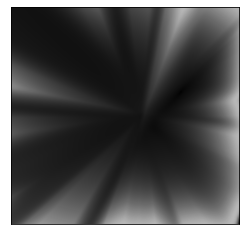
\includegraphics[width=0.8 \textwidth]{sections/006_neurips2020/figures/2D_latent_klpn_1.png}
        \caption{Uncertainty - PriorNet}
        \label{KLPN_visualization_unc}
    \end{subfigure}%
    \begin{subfigure}[t]{0.23 \columnwidth}
        \centering
        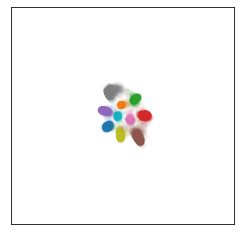
\includegraphics[width=0.8 \textwidth]{sections/006_neurips2020/figures/2D_latent_ours_bn_2.png}
         \caption{Data labels - \PostNetacro}
         \label{ours_visualization_2D}
    \end{subfigure}%
    \begin{subfigure}[t]{0.23\columnwidth}
        \centering
        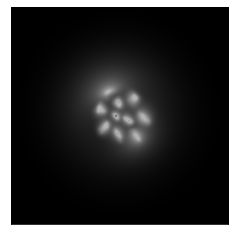
\includegraphics[width=0.8 \textwidth]{sections/006_neurips2020/figures/2D_latent_ours_bn_1.png}
        \caption{Uncertainty - \PostNetacro}
        \label{ours_visualization_unc}
    \end{subfigure}%
    \caption{PriorNet has a pre-ultimate layer of dimension $2$ and was trained with Reverse KL and uniform noise on $[0,255]^{28\times28}$ as OOD data. \PostNetacro has a latent space of dimension $2$ and was trained without OOD data. (a) and (c) show the learned latent positions of data with colored labels. (b) and (d) show uncertainty estimates in the latent spaces where darker regions indicate high uncertainty. \PostNetacro correctly assigns high uncertainty to OOD regions contrary to PriorNet.}
    \label{fig:mnist_2D_latent_space}
	% \vspace{-.5cm}
\end{figure}

\paragraph{Related work.} Uncertainty estimation is a growing research area unifying various approaches \cite{bayesian-networks, simple-baseline-uncertainty, practical_deep_bayesian_principles, Eswaran2017, ensembles, dropout}. Bayesian Neural Networks learn a \emph{distribution} over the weights \cite{bayesian-networks, simple-baseline-uncertainty, practical_deep_bayesian_principles}. Another class of approaches uses a collection of sub-models and aggregates their predictions, which are in turn used to estimate statistics (e.g., mean and variance) of the class probability distribution. Even though such methods, like ensemble and drop-out, have demonstrated remarkable performance (see, e.g., \cite{dataset-shift}), they describe implicit distributions for predictions and require a costly sampling phase at inference time for uncertainty estimation. 

Recently, a new class of models aims to directly predict the parameters of a prior distribution on the categorical probability predictions, accounting for the different types of uncertainty \cite{PriorNetworks, reverse-kl, sensoy2018, uceloss}. However, these methods require (i) the definition of arbitrary target prior distributions \cite{PriorNetworks, reverse-kl, sensoy2018}, and most importantly, (ii) out-of-distribution (OOD) samples during training time, which is an unrealistic assumption in most applications \cite{PriorNetworks, reverse-kl}.

Classically, these models would use both ID and OOD samples (e.g. MNIST and FashionMNIST) during training to detect similar OOD samples (i.e. FashionMNIST) at inference time. We show that preventing access to explicit OOD data during training leads to poor results using these approaches (see Fig.~\ref{fig:mnist_2D_latent_space} for MNIST; or app. for toy datasets). Contrary to the expected results, these models produce increasingly confident predictions for samples far from observed data. In contrast, we propose \PostNet (\PostNetacro), which assigns high epistemic uncertainty to out-of-distribution samples, low overall uncertainty to regions nearby observed data of a single class, and high aleatoric and low epistemic uncertainty to regions nearby observed data of different classes.

\PostNetacro uses normalizing flows to learn a distribution over Dirichlet parameters in latent space. We enforce the densities of the individual classes to integrate to the number of training samples in that class, which matches well with the intuition of Dirichlet parameters corresponding to the number of observations per class. \PostNetacro does not require any OOD samples for training, the (arbitrary) specification of target prior distributions, or costly sampling for uncertainty estimation at test time.

\section{\PostNet}
\label{sec:model_006}

In classification, we can distinguish between two types of uncertainty for a given input $\vect{x}\dataix$: the uncertainty on the class prediction \smash{$y\dataix \in \{1, \ldots, \nclass\}$} (i.e.\ aleatoric unceratinty), and the uncertainty on the categorical distribution prediction \smash{$\vect{p}\dataix = [p\dataix_1, \ldots, p\dataix_\nclass]$} (i.e.\ epistemic uncertainty). A convenient way to model both is to describe the \emph{epistemic distribution} \smash{$q\dataix$} of the categorical distribution prediction \smash{$\vect{p}\dataix$}, i.e.\ \smash{$\vect{p}\dataix \sim q\dataix$}. From the epistemic distribution follows naturally an estimate of the \emph{aleatoric distribution} of the class prediction \smash{$y\dataix \sim \text{Cat}(\bar{\vect{p}}\dataix)$} where \smash{$\E_{q\dataix}[\vect{p}\dataix] = \bar{\vect{p}}\dataix$}.

Approaches like ensembles \cite{ensemble_simple} and dropout \cite{drop_out} model $q\dataix$ implicitly, which only allows them to estimate statistics at the cost of $S$ samples (e.g. \smash{$\E_{q\dataix}[\vect{p}\dataix] \approx \frac{1}{S}\sum_{s=1}^{S} \tilde{\vect{p}}\dataix$} where \smash{$\tilde{\vect{p}}\dataix$} is sampled from \smash{$q\dataix$}). 
%
Another class of models \cite{prior_net, rev_kl_prior_net, uceloss, evidential_uncertainty} explicitly parametrizes the epistemic distribution with a Dirichlet distribution (i.e.\ \smash{$q^{(\idata)} = \text{Dir}(\bm{\alpha}\dataix)$} where \smash{$f_{\theta}(x\dataix) = \bm{\alpha} \dataix \in \mathbb{R}_+^\nclass$}), which is the natural prior for categorical distributions. This parametrization is convenient since it requires only one pass to compute epistemic distribution, aleatoric distribution and class prediction:
\begin{equation}
\begin{aligned}
q^{(\idata)} &= \text{Dir}(\bm{\alpha}\dataix),\hspace{25pt} 
\bar{p}_\iclass\dataix &= \frac{\alpha_\iclass}{\alpha_0} \text{ with } \alpha_0 = \sum^{\nclass}_{\iclass=1} \alpha_\iclass,\hspace{25pt}
y^{(\idata)} &= \arg \max \;[\bar{p}_1, ..., \bar{p}_\nclass]
\end{aligned}
\end{equation}
The concentration parameters \smash{$\alpha\dataix_\iclass$} can be interpreted as the number of observed samples of class $\iclass$ and, thus, are a good indicator of epistemic uncertainty for non-degenerate Dirichlet distributions (i.e.\ \smash{$\alpha\dataix_\iclass \geq 1$}). To learn these parameters, Prior Networks \cite{prior_net, rev_kl_prior_net} use OOD samples for training and define different target values for ID and OOD data. For ID data, \smash{$\alpha\dataix_\iclass$} is set to an arbitrary, large number if $\iclass$ is the correct class and $1$ otherwise. For OOD data, \smash{$\alpha\dataix_\iclass$} is set to $1$ for all classes. 

This approach has four issues:
%\begin{itemize}
    %\item 
    \textbf{(1)} The knowledge of OOD data for training is unrealistic. In practice, we might not have these data, since OOD samples are by definition not likely to be observed.
    %\item 
    \textbf{(2)} Discriminating in- from out-of-distribution data by providing an explicit set of OOD samples is hopeless. Since any data not from the data distribution is OOD, it is therefore impossible to characterize the infinitely large OOD distribution with an explicit data set.
    %\item 
    \textbf{(3)} The predicted Dirichlet parameters can take any value, especially for new OOD samples which were not seen during training. In the same way, the sum of the total fictitious prior observations over the full input domain $\int \alpha_0(\vect{x}) d\vect{x}$  is not bounded and in particular can be much larger than the number of ground-truth observations $N$. This can result in undesired behavior and assign arbitrarily high epistemic certainty for OOD data not seen during training.
    %\item 
    \textbf{(4)} Besides producing such arbitrarily high prior confidence, PNs can also produce degenerate concentration parameters (i.e.\ $\alpha_\iclass$ < 1). While \cite{rev_kl_prior_net} tried to fix this issue by using a different loss, nothing intrinsically prevents Prior Networks from predicting degenerate prior distributions.
%\end{itemize}
In the following section we describe how \PostNet solves these drawbacks.

\subsection{An input-dependent Bayesian posterior}

First, recall the Bayesian update of a single categorical distribution \smash{$y \sim \text{Cat}(\vect{p})$}. It consists in (1) introducing a prior Dirichlet distribution over its parameters i.e. \smash{$\prob(\vect{p}) = \text{Dir}(\bm{\beta^\text{prior}})$} where \smash{$\bm{\beta^\text{prior}} \in \mathbb{R}_+^\nclass$}, and (2) using $N$ given observations \smash{$y^{(1)},..., y^{(N)}$} to form the posterior distribution $\prob(\vect{p}|\{y^{(j)}\}_{j =1}^N)= \text{Dir}(\bm{\beta^\text{prior}} + \bm{\beta^\text{data}})$ where \smash{$\beta^\text{data}_\iclass = \sum_j \mathbb{1}_{y^{(j)}=\iclass}$} are the class counts. That is, the Bayesian update is
\begin{equation}
    \begin{aligned}
    \prob(\vect{p}|\{y^{(j)}\}_{j =1}^n) \propto \prob(\{y^{(j)}\}_{j =1}^n|\vect{p}) \times \prob(\vect{p}).
    \end{aligned}
\end{equation}
Observing no data (i.e. $\beta_\iclass^\text{data} \rightarrow 0$) would lead to flat categorical distribution (i.e. \smash{$p_\iclass = {\beta_\iclass^{\text{prior}}}\cdot ({\sum_{\iclass'}\beta_{\iclass'}^{\text{prior}}})^{-1}$}), while observing many samples (i.e. \smash{$\beta_\iclass^\text{data}$} is large) would converge to the true data distribution (i.e. $p_\iclass \approx \frac{\beta_\iclass}{\sum_i\beta_i}$).
Furthermore, we remark that $N$ behaves like a certainty budget distributed over all classes i.e. \smash{$N = \sum_\iclass \beta^\text{data}_\iclass$}.

Classification is more complex. Generally, we predict the class label \smash{$y\dataix$} from a different categorical distribution \smash{$\text{Cat}(\vect{p}\dataix)$} for each input \smash{$\vect{x}\dataix$}. \PostNetacro extends the Bayesian treatment of a single categorical distribution to classification by predicting an individual posterior update for any possible input. To this end, it distinguishes between a fixed prior parameter \smash{$ \bm{\beta}^{\text{prior}}$} and the additional learned (pseudo) counts \smash{$\bm{\beta}\dataix$} to form the parameters of the posterior Dirichlet distribution \smash{$\bm{\alpha}\dataix = \bm{\beta}^{\text{prior}} + \bm{\beta}\dataix$}. 
%\bc{Remark that directly using the single label \smash{$y\dataix$} to learn independently the posterior for input \smash{$\vect{x}\dataix$ (i.e. $\beta_\iclass\dataix = 1$} for the true class and \smash{$\beta_\iclass\dataix = 0$} otherwise) would lead to a poor uncertainty estimate and more importantly not generalize to new inputs}. 
Hence, \PostNetacro's posterior update is equivalent to predicting a set of pseudo observations \smash{$\{\tilde{y}^{(j)}\}_j\dataix$} per input \smash{$\vect{x}\dataix$}, accordingly \smash{$\beta_\iclass\dataix = \sum_j  \mathbb{1}_{\tilde{y}^{(j)}=\iclass}$} and
\begin{equation}
    \begin{aligned}
    \prob(\vect{p}\dataix|\{\tilde{y}^{(j)}\}_j\dataix) \propto \prob(\{\tilde{y}^{(j)}\}_j\dataix|\vect{p}\dataix) \times \prob(\vect{p}\dataix).
    \end{aligned}
\end{equation}
In practice, we set \smash{$\bm{\beta}^{\text{prior}}=\vect{1}$} leading to a flat equiprobable prior when the model brings no additional evidence, i.e.\ when \smash{$\bm{\beta}\dataix = \vect{0}$}. 

The parametrization of $\beta_\iclass\dataix$ is crucial and based on two main components. The first component is an encoder neural network, $f_{\theta}$ that maps a data point $\vect{x}\dataix$ onto a low-dimensional latent vector $\latent\dataix=f_{\theta}(\vect{x}\dataix) \in \mathbb{R}^{\latentdim}$. The second component is to learn a \textit{normalized} probability density $\prob(\latent | \iclass; \phi)$ per class on this latent space; intuitively acting as class conditionals in the latent space. Given these and the number of ground-truth observations $N_\iclass$ in class  $\iclass$, we define:
\begin{equation}
\begin{aligned}
\label{eq:additional_observations}
	\beta_\iclass\dataix &= N_\iclass \cdot \prob(\latent\dataix | c; \phi) = N \cdot \prob(\latent\dataix | \iclass; \phi) \cdot \prob(\iclass),
\end{aligned}
\end{equation}
which corresponds to the number of (pseudo) observations of class $\iclass$ at $\latent \dataix$. Note that it is crucial that $\prob(\latent | \iclass; \phi)$ corresponds to a proper normalized density function since this will ensure the model's epistemic uncertainty to increase outside the known distribution. Indeed, the core idea of our approach is to parameterize these distributions by a flexible, yet tractable family: normalizing flows (e.g. radial flow \cite{vi_flow} or IAF \cite{iaf_flow}). Note that normalizing flows are theoretically capable of modeling any continuous distribution given an expressive and deep enough model \cite{neural_flow, iaf_flow}.

In practice, we observed that various architectures can be used for the encoder. Also, similarly to GAN training \cite{GAN_batch_norm}, we observed that adding a batch normalization after the encoder made the training more stable. It facilitates the match between the latent positions output by the encoder and non-zero density regions learned by the normalizing flows. Remark that we can theoretically use any density estimator on the latent space. We experimentally compared Mixtures of Gaussians (MoG), radial flow \cite{vi_flow} and IAF \cite{iaf_flow}. While all density types performed reasonably well (see Tab.~\ref{fig:unc_sensorless_drive} and app.), we observed a better performance of flow-based density estimation in general. We decided to use radial flow for its good trade-off between flexibility, stability, and compactness (only few parameters).

\textbf{Model discussion.} Equation \ref{eq:additional_observations} exhibits a set of interesting properties which ensure reasonable uncertainty estimates for ID and OOD samples. To highlight the properties of the Dirichlet distributions learned by \PostNetacro, we assume in this paragraph that we have a fixed encoder $f_\theta$ and normalizing flow model parameterized by $\phi$. Writing the mean of the Dirichlet distribution parametrized by \eqref{eq:additional_observations} and using Bayes' theorem gives:
\begin{equation}
\E_{\vect{p}\sim \Dir(\boldsymbol{\alpha}\dataix)}[p_\iclass] = \frac{\beta_\iclass^\text{prior} + N \cdot \prob(\iclass | \latent\dataix; \phi) \cdot \prob(\latent\dataix; \phi)}{\sum_\iclass\beta_\iclass^\text{prior} + N \cdot \prob(\latent\dataix; \phi)}
\end{equation}
For very likely in-distribution data (i.e. $\prob(\latent\dataix ; \phi) \rightarrow \infty$), the aleatoric distribution estimate \smash{$\bar{\vect{p}}\dataix = \E_{\vect{p}\sim \Dir(\boldsymbol{\alpha}\dataix)}[p_\iclass]$} converges to the true categorical distribution \smash{$\prob(\iclass|\latent \dataix; \phi)$}. Thus, predictions are more accurate and calibrated for likely samples. Conversely, for out-of-distribution samples (i.e. \smash{$\prob(\latent\dataix ; \phi) \rightarrow 0$}), the aleatoric distribution estimate \smash{$\bar{\vect{p}}\dataix = \E_{\vect{p}\sim \Dir(\boldsymbol{\alpha}\dataix)}[p_\iclass]$} converges to the flat prior distribution (e.g. \smash{$p_\iclass=\frac{1}{\nclass}$} if \smash{$\bm{\beta}^{prior}=\vect{1}$}). In the same way, we show in the appendix that the covariance of the epistemic distribution converges to $\vect{0}$ for very likely in-distribution data, meaning no epistemic uncertainty. Thus, uncertainty for in-distribution data is reduced to the (inherent) aleatoric uncertainty and zero epistemic uncertainty.
%
Similarly to the single categorical distribution case, increasing the training dataset size (i.e. $N \rightarrow \infty$) also leads to the mean prediction $\E_{\vect{p}\sim \Dir(\boldsymbol{\alpha})}[p_\iclass]$ converging to the class posterior \smash{$\prob(c | \latent\dataix; \phi)$}. On the contrary, no observed data (i.e $N=0$) again leads to the model reverting to a flat prior.

\PostNet also handles limited certainty budgets at different levels. At the sample level, the certainty budget \smash{$\alpha_0\dataix = \sum_\iclass \alpha_\iclass\dataix$} is distributed over classes. At the class level, the certainty budget \smash{$N_\iclass = \int N_\iclass \; \prob(\latent | c; \phi) \; d\latent = N_\iclass  \int \prob(\latent | c; \phi) \; d\latent$} is distributed over samples. At the dataset level, the certainty budget \smash{$N = \sum_\iclass \int N_\iclass \; \prob(\latent | c; \phi) \; d\latent$} is distributed over classes and samples. Regions of latent space with many training examples are assigned high density $\prob(\latent | c; \phi)$, forcing low density elsewhere to fulfill the integration constraint. Consequently, density estimation using normalizing flows enables \PostNetacro to learn out-of-distribution uncertainty by observing only in-distribution data.

\begin{wrapfigure}[16]{r}{0.505\textwidth}
    \vspace{-.3cm}
	\resizebox{.505 \columnwidth}{!}{
	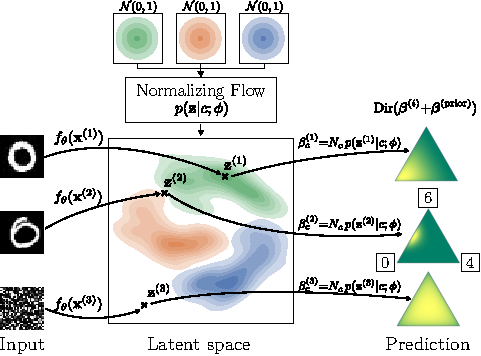
\includegraphics{sections/006_neurips2020/diagram/diagram_new-crop.pdf}
	}
	\caption{Overview of \PostNet.}
	\label{fig:overview}
	\vspace{-.5cm}
\end{wrapfigure}

\textbf{Overview.} In Figure~\ref{fig:overview} we provide an overview of \PostNet. We have three example inputs, \smash{$\vect{x}^{(1)}$,} \smash{$\vect{x}^{(2)}$}, and \smash{$\vect{x}^{(3)}$}, which are mapped onto their respective latent space coordinates $\latent\dataix$ by the encoding neural network $f_\theta$. The normalizing flow component learns flexible (normalized) density functions $\prob(\latent|c;\phi)$, for which we evaluate their densities at the positions of the latent vectors \smash{$\latent\dataix$}. These densities are used to parameterize a Dirichlet distribution for each data point, as seen on the right hand side. Higher densities correspond to higher confidence in the Dirichlet distributions -- we can observe that the out-of-distribution sample \smash{$\vect{x}^{(3)}$} is mapped to a point with (almost) no density, and hence its predicted Dirichlet distribution has very high epistemic uncertainty. On the other hand, \smash{$\vect{x}^{(2)}$} is an ambiguous example that could depict either the digit 0 or 6. This is reflected in its corresponding Dirichlet distribution, which has high aleatoric uncertainty (as the sample is ambiguous), but low epistemic uncertainty (since it is from the distribution of hand-drawn digits). The unambiguous sample \smash{$\vect{x}^{(1)}$} has low overall uncertainty.

Lastly, since both the encoder network $f_\theta$ and the normalizing flow parameterized by $\phi$ are fully differentiable, we can learn their parameters jointly in an end-to-end fashion. We do this via a novel loss  defined in Sec.\ref{sec:uncertainty_loss_006} which emerges from Bayesian learning principles \cite{PAC_bayesian_estimator} and is related to \UCEacro \cite{uceloss}.

\subsection{Density estimation for OOD detection}

Normalized densities, as used by \PostNetacro, are well suited to discriminate between ID data (with high likelihoood) and OOD data (with low likelihood). While it is also possible to learn a normalizing flow model on the input domain directly (e.g., \cite{NIPS2017_6828, NIPS2018_8224, grathwohl2018scalable}), this is very computationally demanding and might not be necessary for a discriminative model. Futhermore, density estimation is prone to the curse of dimensionality in high dimensional spaces \cite{typicality_OOD_generative, waic_robust_anomaly_detection}. For example, unsupervised deep generative models like \cite{glow} or \cite{pixel_cnn} have been shown to be unable to distinguish between ID and OOD samples in some situations when working on all features directly \cite{deep_generative_do_not_know, energy_based_classifier}. 

To circumvent these issues, \PostNetacro leverages two techniques. First, it uses the full class label information. Thus, \PostNetacro assigns a density per class and regularizes the epistemic uncertainty with the training class counts $N_\iclass$. Second, \PostNetacro performs density estimation on a low dimensional latent space describing relevant features for the classification task (Fig.~\ref{fig:mnist_2D_latent_space}; Fig.~\ref{fig:overview}).
Hence, \PostNetacro does not suffer from the curse of dimensionality and still enjoys the benefits of a properly normalized density function. Using the inductive bias of a discriminative task and low dimensional latent representations improved OOD detection in  \cite{nf_fail_ood} as well.

\section{Uncertainty-Aware Loss Computation}
\label{sec:uncertainty_loss_006}

A crucial design choice for neural network learning is the loss function. \PostNetacro estimates both aleatoric and epistemic uncertainty by learning a distribution $q\dataix$ for data point $\idata$ which is close to the true posterior of the categorical distribution $\vect{p}\dataix$ given the training data $\vect{x}\dataix$:
%\begin{equation}
    $q(\vect{p}\dataix) \simeq \prob(\vect{p}\dataix | \vect{x}\dataix)$.
%\end{equation}
One way to approximate the posterior is the following Bayesian loss function \cite{update-belief-propagation,PAC-bayesian_estimator,opt_info_processing_bayes}, which has the nice property of being optimal when $q\dataix$ is equal to the true posterior distribution:
\begin{equation}
\label{general_bayesian_loss}
    q^* = \underset{q\dataix \in \mathcal{P}}{\arg \min}\; \E_{\psi\dataix \sim q(\psi\dataix)}[l(\psi\dataix, \vect{x}\dataix)] - H(q\dataix),
\end{equation}
where $l$ is a generic loss over \smash{$\psi\dataix$} satisfying \smash{$ 0 < \int \exp(-l(\psi, x)) d\psi < \infty$, $\mathcal{P}$} is the family of distributions we consider and \smash{$H(q\dataix)$} denotes the entropy of $q\dataix$.

Applied in our case, \PostNet learns a distribution $q$ from the family of the Dirichlet distributions \smash{$\text{Dir}(\bm{\alpha}\dataix) = \mathcal{P}$} over the parameters \smash{$\vect{p}\dataix = \psi\dataix$}. Instantiating the loss $l$ with the cross-entropy loss (CE) we obtain the following optimization objective
\begin{equation}
\label{dirichlet_bayesian_loss}
       \min_{\theta,\phi} \mathcal{L} = \min_{\theta, \phi} \frac{1}{N} \sum_{\idata}^{N} \underbrace{\E_{q(\mathbf{p}\dataix)}[\text{CE}(\mathbf{p}\dataix, \vect{y}\dataix)]}_{\text{(1)}} - \underbrace{H(q\dataix)}_{\text{(2)}}
\end{equation}
where $\mathbf{y}\dataix$ corresponds to the one-hot encoded ground-truth class of data point $i$.
Optimizing this loss approximates the true posterior distribution for the the categorical distribution $\vect{p}\dataix$. The first term (1) corresponds the \UCE (\UCEacro) introduced by \cite{uceloss}, which is known to increase confidence for observed data. The second term (2) is an entropy regularizer, which emerges naturally and favors smooth distributions $q\dataix$. Here we are optimizing jointly over the neural network parameters $\theta$ and $\phi$. We also experimented with sequential training i.e. optimizing over the normalizing flow component only with a pre-trained model (see \cref{fig:ablation_sensorless_drive} and app.). Once trained, \PostNetacro can predict uncertainty-aware Dirichlet distributions for unseen data points.

Observe that \cref{dirichlet_bayesian_loss} is equivalent to the ELBO loss used in variational inference when using a uniform Dirichlet prior (i.e. $(1)=-\E_{q(\mathbf{p}\dataix)}[\log \prob(\vect{y}\dataix|\mathbf{p}\dataix)]$ and $(2)=\text{KL}(q\dataix||\prob(\mathbf{p}\dataix))$ where $\prob(\mathbf{p}\dataix) = \text{Dir}(\mathbf{1})$). The more general \cref{general_bayesian_loss}, however, is not necessarily equal to an ELBO loss.

Another interesting special case is to consider the family of Dirac distributions as \smash{$\mathcal{P}$} instead of the family of Dirichlet distributions. In this case we find back the traditional cross-entropy loss, which performs a simple point estimate for the distribution $\vect{p}\dataix$. CE is therefore not suited to learn a distribution with non-zero variance, as explained in \cite{uceloss}.

Other approaches, such as dropout, approximate the expectation in \UCEacro by sampling from \smash{$q\dataix$}. Our approach has the advantage of using closed-form expressions both for \UCEacro \cite{uceloss} and the entropy term, thus being efficient and exact. The weight of the entropy regularization is a hyperparameter; experiments have shown \PostNetacro to be fairly insensitive to it, so in our experiments we set it to \smash{$10^{-5}$}.

\section{Experimental Evaluation}
\label{sec:experiments_006}

In this section we compare our model to previous methods on a rich set of experiments. The code and further supplementary material is available online (\url{www.daml.in.tum.de/postnet}).

\paragraph{Baselines.} We have special focus on comparing with other models parametrizing Dirichlet distributions. We use Prior Networks (PN) trained with KL divergence (\textbf{KL-PN}) \cite{PriorNetworks} and Reverse KL divergence (\textbf{RKL-PN}) \cite{reverse-kl}. These methods assume the knowledge of in- and out-of-distribution samples. For fair evaluation, the actual OOD test data cannot be used; instead, we used uniform noise on the valid domain as OOD training data. Additionally we trained RKL-PN with FashionMNIST as OOD data for MNIST (\textbf{RKL-PN w/ F.}). We also compare to Distribution Distillation (\textbf{Distill.}) \cite{distribution-distillation}, which learns Dirichlet distributions with maximum likelihood by using soft-labels from an ensemble of networks. 
As further baselines, we compare to dropout models (\textbf{Dropout Net}) \cite{dropout} and ensemble methods (\textbf{Ensemble Net}) \cite{ensembles}, which are state of the art in many tasks involving uncertainty estimation \cite{dataset-shift}. Empirical estimates of the mean and variance of \smash{$q\dataix$} are computed based on the neuron drop probability $p_{\text{drop}}$, and $m$ individually trained networks for ensemble.

All models share the same core architecture using 3 dense layers for tabular data, and 3 conv. + 3 dense layers for image data. Similarly to \cite{PriorNetworks, reverse-kl}, we also used the VGG16 architecture \cite{vgg} on CIFAR10. We performed a grid search on $p_{\text{drop}}$, $m$, learning rate and hidden dimensions, and report results for the best configurations. Results are obtained from 5 trained models with different initializations.
Moreoever, for all experiments, we split the data into train, validation and test set  ($60\%$, $20\%$, $20\%$) and train/evaluate all models on $5$ different splits. Besides the mean we also report the standard error of the mean. Further details are given in the appendix.

\paragraph{Datasets.} We evaluate on the following real-world datasets: \textbf{Segment} \cite{uci_datasets}, \textbf{Sensorless Drive} \cite{uci_datasets}, \textbf{MNIST} \cite{mnist} and \textbf{CIFAR10} \cite{cifar10}. The former two datasets (Segment and Sensorless Drive) are tabular datasets with %unbounded input domain of 
dimensionality 18 and 49 and with 7 and 11 classes, respectively. We rescale all inputs between $[0, 1]$ by using the $\min$ and $\max$ value of each dimension from the training set. Additionally, we compare all models on 2D synthetic data composed of three Gaussians each. Datasets are presented in  more detail in the appendix.

\paragraph{Metrics.} We follow the method proposed in \cite{dataset-shift} and evaluate the coherence of confidence, uncertainty calibration and OOD detection. Note that our goal is not to improve accuracy; still we report the numbers in the experiments.

\underline{Confidence calibration:} We aim to answer `\textit{Are more confident (i.e. less uncertain) predictions more likely to be correct?}'. We use the area under the precision-recall curve (AUC-PR) to measure confidence calibration. For aleatoric confidence calibration (\textbf{Alea. Conf.}) we use \smash{$\underset{\iclass}{\max} \; \bar{\vect{p}}_\iclass\dataix$} as the scores with labels 1 for correct and 0 for incorrect predictions. For epistemic confidence calibration (\textbf{Epist. Conf.}), we distinguish Dirichlet-based models, and dropout and ensemble models. For the former we use \smash{$\underset{\iclass}{\max}\; \bm{\alpha}_\iclass\dataix$} as scores, and for the latter we use the (inverse) empirical variance \smash{$\tilde{\vect{p}}_c\dataix$} of the predicted class, estimated from 10 samples.

\underline{Uncertainty calibration:} We used Brier score (\textbf{Brier}), which is computed as $\frac{1}{N}\sum_{i}^N \|\bar{\vect{p}}\dataix - \vect{y}\dataix\|_2$, where $\vect{y}\dataix$ is the one-hot encoded ground-truth class of data point $i$. For Brier score, lower is better.

\underline{OOD detection:} Our main focus lies on the models' ability to detect out-of-distribution samples. We used AUC-PR to measure performance. For aleatoric OOD detection (\textbf{Alea. OOD}), the scores are \smash{$\underset{\iclass}{\max} \; \bar{\vect{p}}_\iclass\dataix$} with labels 1 for ID data and 0 for OOD data. Fo epistemic OOD detection (\textbf{Epist. OOD}), the scores for Dirichlet-based models are given by \smash{$\alpha_0\dataix = \sum_\iclass \alpha_\iclass\dataix$}, while we use the (inverse) empirical variance \smash{$\tilde{\vect{p}}\dataix$} for ensemble and dropout models. To provide a comprehensive overview of OOD detection results we use different types of OOD data as described in the following: 
\begin{itemize}
    \item \textit{Unseen datasets.} We use data from other datasets as OOD data for the image-based models. We use data from FashionMNIST \cite{fashionmnist} and K-MNIST \cite{kmnist}  as OOD data for models trained on MNIST, and data from SVHN \cite{svhn} as OOD for CIFAR10.
    \item \textit{Left-out classes.} For the tabular datasets (Segment and Sensorless Drive) there are no other datasets that are from the same domain. To simulate OOD data we remove one or more classes from the training data and instead consider them as OOD data. We removed one class (class sky) from the Segment dataset and two classes from Sensorless Drive (class 10 and 11).
    \item \textit{Out-of-domain.} In this novel evaluation we consider an extreme case of OOD data for which the data comes from different value ranges (\textbf{OODom}). E.g., for images we feed unscaled versions in the range $[0, 255]$ instead of scaled versions in $[0,1]$. We argue that models should easily be able to detect data that is extremely far from the data distribution. However, as it turns out, this is surprisingly difficult for many baseline models.
    \item \textit{Dataset shifts.} Finally, for CIFAR10, we use 15 different image corruptions at 5 different severity levels \cite{benchmarking-corruptions}. This setting evaluates the models' ability to detect low-quality data (\cref{cifar_shifts}b,c). 
\end{itemize}

\begin{table}
    \centering
    \resizebox{.9 \textwidth}{!}{%
\begin{tabular}{lllllll}
\toprule
{} &  \textbf{Acc.} & \textbf{Alea. Conf.} & \textbf{Epist. Conf.} & \textbf{Brier} & \textbf{OOD Alea.} & \textbf{OOD Epist.} \\
\midrule
\midrule
\textbf{Drop Out  } &  89.32$\pm$0.2 &        98.21$\pm$0.1 &         95.24$\pm$0.2 &  28.86$\pm$0.4 &      35.41$\pm$0.4 &       40.61$\pm$0.7 \\
\textbf{Ensemble  } &  99.37$\pm$0.0 &        99.99$\pm$0.0 &         *99.98$\pm$0.0 &   2.47$\pm$0.1 &      50.01$\pm$0.0 &       50.62$\pm$0.1 \\
\midrule
\textbf{Distill.  } &  93.66$\pm$1.5 &        98.29$\pm$0.5 &         98.15$\pm$0.5 &  44.94$\pm$1.4 &       32.1$\pm$0.6 &       31.17$\pm$0.2 \\
\textbf{KL-PN     } &  94.77$\pm$0.9 &        99.52$\pm$0.1 &         99.47$\pm$0.1 &  21.47$\pm$1.9 &      35.48$\pm$0.8 &        33.2$\pm$0.6 \\
\textbf{RKL-PN    } &  99.42$\pm$0.0 &        99.96$\pm$0.0 &         99.89$\pm$0.0 &   9.07$\pm$0.1 &      45.89$\pm$1.6 &       38.14$\pm$0.8 \\
\textbf{PostN Rad.} &  98.02$\pm$0.1 &        99.89$\pm$0.0 &         99.47$\pm$0.0 &   5.51$\pm$0.2 &      72.89$\pm$0.8 &       \textbf{*88.73$\pm$0.5} \\
\textbf{PostN IAF } &  \textbf{*99.52$\pm$0.0} &        \textbf{*100.0$\pm$0.0} &         \textbf{99.92$\pm$0.0}&   \textbf{*1.43$\pm$0.1} &      \textbf{*82.96$\pm$0.8} &       88.65$\pm$0.4 \\
\bottomrule
\end{tabular}

    }
    \caption{Results on Sensorless Drive dataset. Bold numbers indicate best score among Dirichlet parametrized models and starred numbers indicate best scores among all models.}
    \label{fig:unc_sensorless_drive}
%\vspace{-.0cm}
\end{table}

\textbf{Results.} 
Results for the Sensorles Drive dataset are shown in \cref{fig:unc_sensorless_drive}. Tables for other datasets are in the appendix. Even without requiring expensive sampling, \PostNetacro performs on par for accuracy and confidence scores with other models, brings a significant improvement for calibration within the Dirichlet-based models, and outperforms all other models by a large margin (more than $+30\%$ abs. improvement) for OOD detection. Radial flow and IAF variants both achieve strong performance for all datasets (see \cref{sec:app_additional_results}). We use the smaller model (i.e. Radial flow) for comparison in the following. In our experiments, note that using one Radial flow per class represents a small overhead of only $80$ parameters per class, which is negligible compared to the encoder architectures (e.g. VGG16 has 138M parameters).

\begin{figure}
    \centering
    \begin{subfigure}[t]{0.33 \textwidth}
        \centering
        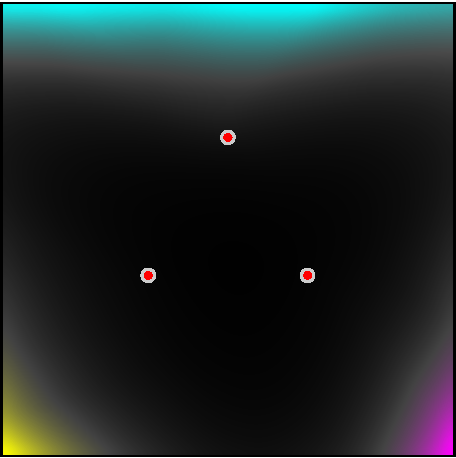
\includegraphics[width=0.5 \textwidth]{sections/006_neurips2020/figures/three_gaussians_no_flow-crop.pdf}
        \caption{\PostNetacro: \NoFlow}
    \end{subfigure}%   
    \begin{subfigure}[t]{0.33 \textwidth}
        \centering
        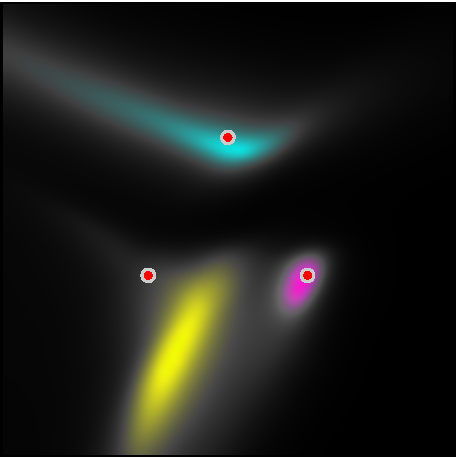
\includegraphics[width=0.5 \textwidth]{sections/006_neurips2020/figures/three_gaussians_no_UCE-crop.pdf}
        \caption{\PostNetacro: \NoUCE}
    \end{subfigure}%   
    \begin{subfigure}[t]{0.33 \textwidth}
        \centering
        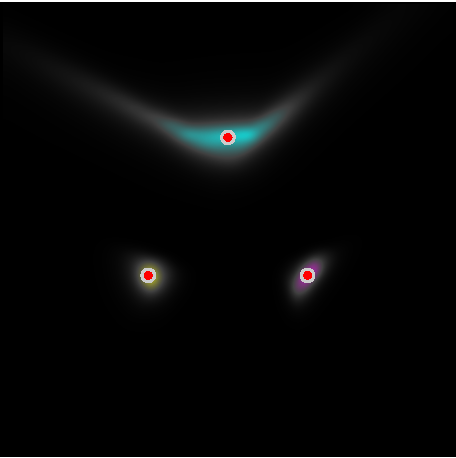
\includegraphics[width=0.5 \textwidth]{sections/006_neurips2020/figures/three_gaussians_normal-crop.pdf}
        \caption{\PostNetacro: Complete}
    \end{subfigure}%

    \caption{Uncertainty visualization for a 2D 3-Gaussians dataset. Red dots indicate the Gaussians means. Darker regions indicate high epistemic uncertainty for a class prediction. Ablated models fail even a simple dataset while \PostNetacro shows high certainty around gaussians means only.}
    \label{fig:toy_ablation}
	%\vspace{-.0cm}
\end{figure}

\begin{table}[H]
\resizebox{1 \textwidth}{!}{%
\begin{tabular}{lllllll}
\toprule
{} &  \textbf{Acc.} & \textbf{Alea. Conf.} & \textbf{Epist. Conf.}  & \textbf{Brier} & \textbf{OOD Alea.} & \textbf{OOD Epist.} \\
\midrule
\midrule
\textbf{PostN: No-Flow        } &  \cellcolor{Gray} 55.38$\pm$0.7 & \cellcolor{Gray} 85.46$\pm$0.3 & \cellcolor{Gray} 82.58$\pm$0.6 & \cellcolor{Gray} 64.4$\pm$0.6 & \cellcolor{Gray} 29.59$\pm$0.1 & \cellcolor{Gray} 31.15$\pm$0.4 \\
\textbf{PostN: No-Bayes-Loss} &   96.6$\pm$0.2 & 99.74$\pm$0.0 & 98.68$\pm$0.1 & \cellcolor{Gray} 8.85$\pm$0.4 & \cellcolor{Gray} 62.39$\pm$1.5 & \cellcolor{Gray} 82.63$\pm$1.4 \\
\textbf{PostN: Seq-No-Bn   } &  \cellcolor{Gray} 15.09$\pm$1.0 & \cellcolor{Gray} 39.88$\pm$7.2 &  \cellcolor{Gray}  39.86$\pm$7.2 &  \cellcolor{Gray} 89.88$\pm$1.3 & \cellcolor{Gray} 57.19$\pm$2.5 & \cellcolor{Gray} 56.74$\pm$2.4 \\
\textbf{PostN: Seq-Bn    } &  98.42$\pm$0.1 & 99.92$\pm$0.0 & 98.76$\pm$0.1 &   5.41$\pm$0.1 & \cellcolor{Gray} 52.35$\pm$0.7 &  \cellcolor{Gray} 71.75$\pm$1.9 \\
\bottomrule
\end{tabular}

    }
    \caption{Ablation study results on Sensorless Drive dataset. Gray cells indicate significant drops in scores compared to complete \PostNetacro Rad. in \cref{fig:unc_sensorless_drive}.}
        \label{fig:ablation_sensorless_drive}
    % \vspace{-.5cm}
\end{table}

We performed an ablation study on each component of \PostNetacro to evaluate their individual contributions. We were especially interested in comparing stability and uncertainty estimates. Thus, we removed independently the normalizing flow component (\NoFlow) and the novel Bayesian loss (\NoUCE) replaced by the classic cross-entropy loss. Furthermore, we used pre-trained models and subsequently only trained the normalizing flow component, with or without a batch normalization layer (\SeqBn and \SeqNoBn). We report results in \cref{fig:ablation_sensorless_drive}. \NoFlow has a significant drop in OOD detection scores similarly to Prior Networks; not surprising since they mainly differ by their loss. This underlines the importance of using normalized density estimation to differentiate ID and OOD data. The lower performance of \NoUCE compared to the original model indicates the benefit of using our Bayesian loss.
 \SeqBn obtains good performance for some of the metrics, which as a by-product, allows to estimate uncertainty on pre-trained models. Though, we noticed better performance for joint training in general. As shown by \SeqNoBn scores, the batch normalization layer brings stability. It intuitively facilitates predicted latent positions to lie on non-zero density regions. Similar conclusions can be drawn on the toy dataset (see \cref{fig:toy_ablation}) and the Segment dataset (see \cref{sec:app_additional_results}). We further compare various density types and latent dimensions in appendix. We noticed that a too high latent dimension leads to a performance decrease. We also observed that flow-based density estimation generally achieves better scores.

\begin{table}[H]
    \resizebox{1 \textwidth}{!}{%
\begin{tabular}{lllllllll}
\toprule
{} & \textbf{OOD K.} & \textbf{OOD K.} & \textbf{OOD F.} & \textbf{OOD F.} & \textbf{OODom K.} & \textbf{OODom K.} & \textbf{OODom F.} & \textbf{OODom F.} \\
{} & \textbf{Alea.} & \textbf{Epist.} & \textbf{Alea.} & \textbf{Epist.} & \textbf{Alea.} & \textbf{Epist.} & \textbf{Alea.} & \textbf{Epist.} \\
\midrule
\midrule
\textbf{RKL-PN      } &         60.76$\pm$2.9 &          53.76$\pm$3.4 &         78.45$\pm$3.1 &          72.18$\pm$3.6 &            9.35$\pm$0.1 &             8.94$\pm$0.0 &            9.53$\pm$0.1 &             8.96$\pm$0.0 \\
\textbf{RKL-PN w/ F.} &         81.34$\pm$4.5 &          78.07$\pm$4.8 &         \textbf{100.0$\pm$0.0} &          \textbf{100.0$\pm$0.0} &            9.24$\pm$0.1 &             9.08$\pm$0.1 &           88.96$\pm$4.4 &            87.49$\pm$5.0 \\
\textbf{PostN       } &         \textbf{95.75$\pm$0.2} &          \textbf{94.59$\pm$0.3} &         97.78$\pm$0.2 &          97.24$\pm$0.3 &           \textbf{100.0$\pm$0.0} &            \textbf{100.0$\pm$0.0} &           \textbf{100.0$\pm$0.0} &            \textbf{100.0$\pm$0.0} \\
\bottomrule
\end{tabular}

    }
    \caption{Results on MNIST for OOD detection against KMNIST (K.) and FashionMNIST (F.). We trained Rev. KL divergence PriorNets with uniform noise (RKL-PN) and Fashion MNIST (RKL-PN w/ F.) as OOD. \PostNetacro requires no OOD data. Larger numbers are better.}
    \label{fig:unc_MNIST}
    % \vspace{-.5cm}
\end{table}

Results of the comparison between RKL-PN, RKL-PN w/ F and \PostNetacro for OOD detection on MNIST are shown in \cref{fig:unc_MNIST}. Not surprisingly, the usage of FashionMNIST as OOD data for training helped RKL-PN to detect other FashionMNIST data. Except for FashionMNIST OOD, \PostNetacro still outperforms RKL-PN w/ F. in OOD detection for other datasets. We noticed that tabular datasets, defined on an unbounded input domain, are more difficult for baselines. One explanation is that due to the $\min$/$\max$ normalization it can happen that test samples lie outside the interval $[0,1]$ observed during training. For images, the input domain is compact, which allows to define a valid distribution for OOD data (e.g. uniform) which makes OODom data challenging (see OOD vs OODom in \cref{fig:unc_MNIST}).

\begin{table}[H]
    \resizebox{1 \textwidth}{!}{%
\begin{tabular}{lllllllll}
\toprule
{} &  \textbf{Acc.} & \textbf{Alea. Conf.} & \textbf{Epist. Conf.}  & \textbf{Brier} & \textbf{OOD Alea.} & \textbf{OOD Epist.} & \textbf{OODom Alea.} & \textbf{OODom Epist.} \\
\midrule
\midrule
\textbf{Drop Out C.} &  71.73$\pm$0.2 &        92.18$\pm$0.1 &          84.38$\pm$0.3 &  49.76$\pm$0.2 &      \textbf{72.94$\pm$0.3} &       41.68$\pm$0.5 &         28.3$\pm$1.8 &          47.1$\pm$3.3 \\
\textbf{KL-PN C.   } &  48.84$\pm$0.5 &        78.01$\pm$0.6 &          77.99$\pm$0.7 &  83.11$\pm$0.6 &      59.32$\pm$1.1 &       58.03$\pm$0.8 &        17.79$\pm$0.0 &         20.25$\pm$0.2 \\
\textbf{RKL-PN C.  } &  62.91$\pm$0.3 &        85.62$\pm$0.2 &          81.73$\pm$0.2 &  58.12$\pm$0.4 &      67.07$\pm$0.4 &       56.64$\pm$0.8 &        17.83$\pm$0.0 &         17.76$\pm$0.0 \\
\textbf{PostN C.   } &  \textbf{76.46$\pm$0.3} &        \textbf{94.75$\pm$0.1} &          \textbf{94.34$\pm$0.1} &  \textbf{37.39$\pm$0.4} &      72.83$\pm$0.6 &       \textbf{72.82$\pm$0.7} &        \textbf{100.0$\pm$0.0} &         \textbf{100.0$\pm$0.0} \\
\midrule
\textbf{Drop Out V.} &  82.84$\pm$0.1 &        97.15$\pm$0.0 &           96.6$\pm$0.0 &  27.15$\pm$0.2 &      51.39$\pm$0.1 &       53.64$\pm$0.1 &        51.38$\pm$0.1 &         53.66$\pm$0.1 \\
\textbf{KL-PN V.   } &  27.46$\pm$1.7 &        50.61$\pm$4.0 &          52.49$\pm$4.2 &  87.28$\pm$1.0 &      43.96$\pm$1.9 &       43.23$\pm$2.3 &        18.14$\pm$0.1 &         19.12$\pm$0.4 \\
\textbf{RKL-PN V.  } &  64.76$\pm$0.3 &        86.11$\pm$0.4 &          85.59$\pm$0.3 &  54.73$\pm$0.4 &      53.61$\pm$1.1 &       49.37$\pm$0.8 &        29.07$\pm$2.1 &         24.84$\pm$1.3 \\
\textbf{PostN V.   } &  \textbf{84.85$\pm$0.0} &        \textbf{97.76$\pm$0.0} &          \textbf{97.25$\pm$0.0} &  \textbf{22.84$\pm$0.0} &      \textbf{80.21$\pm$0.2} &       \textbf{77.71$\pm$0.3} &        \textbf{91.35$\pm$0.5} &         \textbf{99.25$\pm$0.1} \\
\bottomrule
\end{tabular}

    }
    \caption{Results on CIFAR10 with simple convolutional architectures (C.) and VGG16 (V.). Bold numbers indicate best score among one architecture type.}
    \label{fig:unc_CIFAR10}
    % \vspace{-.5cm}
\end{table}

Uncertainty estimation should be good regardless of the model accuracy. It is even more important for less accurate models since they actually \emph{do not know} (i.e.\ they do more mistakes). Thus, we compared the models that use a single network for training (using a convolutional architecture and VGG16) in \cref{fig:unc_CIFAR10}. Without the knowledge of true OOD data (SVHN) during training, Prior Networks struggle to achieve good performance. In contrast, \PostNetacro outputs high quality uncertainty estimates regardless of the architecture used for the encoder. We report additional results for PostNet using other encoder architectures (convolutional architecture, AlexNet \cite{alexnet}, VGG \cite{vgg} and ResNet \cite{resnet}) in \cref{tab:architecture_CIFAR10}. Deep generative models as Glow \cite{glow} using density estimation on input space are unable to distinguish between CIFAR10 and SVHN \cite{deep-generative}. In contrast, \PostNetacro clearly distinguishes between in-distribution data (CIFAR10) with low entropy, out-of-distribution (OOD SVHN) with high entropy, and close to the maximum possible entropy for out-of-domain data (OODom SVHN) (see \cref{cifar_shifts}a). Similar conclusions hold for MNIST and FashionMNIST (see \cref{sec:app_additional_results}). Furthermore, results for the image perturbations on CIFAR10 introduced by \cite{benchmarking-corruptions} are presented in \cref{cifar_shifts}.  We define the average change in confidence as the ratio between the average confidence \smash{$\frac{1}{N}\sum_i^{N}\alpha_0\dataix$} at severity 1 vs other severity levels. As larger shifts correspond to larger differences in the underlying distributions, we expect uncertainty-aware models to become less certain for more severe perturbations. \PostNet exhibits, as desired, the largest decrease in confidence with stronger corruptions (see \cref{cifar_shifts}b) while maintaining a high accuracy (see \cref{cifar_shifts}c).

\begin{table}[ht]
    \resizebox{1 \textwidth}{!}{%
\begin{tabular}{lllllllll}
\toprule
{} &  \textbf{Acc.} & \textbf{Alea. Conf.} & \textbf{Epist. Conf.}  & \textbf{Brier} & \textbf{OOD Alea.} & \textbf{OOD Epist.} & \textbf{OODom Alea.} & \textbf{OODom Epist.} \\
\midrule
\textbf{\PostNetacro: Conv.  } &  78.58$\pm$0.1 &        95.45$\pm$0.0 &          93.36$\pm$0.0 &  33.84$\pm$0.2 &      72.21$\pm$0.1 &       57.72$\pm$0.7 &        100.0$\pm$0.0 &         100.0$\pm$0.0 \\
\textbf{\PostNetacro: Alexnet} &  80.81$\pm$0.2 &        96.33$\pm$0.1 &          95.35$\pm$0.1 &  29.99$\pm$0.3 &       73.4$\pm$0.7 &       67.05$\pm$0.6 &        97.64$\pm$0.4 &         99.64$\pm$0.1 \\
\textbf{\PostNetacro: VGG    } &  84.85$\pm$0.0 &        97.76$\pm$0.0 &          97.25$\pm$0.0 & 22.84$\pm$0.0 &      80.21$\pm$0.2 &       77.71$\pm$0.3 &        91.35$\pm$0.5 &         99.25$\pm$0.1 \\
\textbf{\PostNetacro: Resnet } &  87.86$\pm$0.2 &        98.35$\pm$0.0 &          97.13$\pm$0.0 &  19.33$\pm$0.3 &      79.92$\pm$0.4 &       72.25$\pm$0.6 &        99.94$\pm$0.0 &         99.94$\pm$0.0 \\
\bottomrule
\end{tabular}

    }
    \caption{Results of \PostNetacro with different encoder architectures. It shows good uncertainty estimation regardless of the architecture complexity.}
    \label{tab:architecture_CIFAR10}
\end{table}

\begin{figure}[H]
    % \vspace{-.5cm}
    \centering
    \begin{subfigure}[t]{0.33 \textwidth}
        \centering
        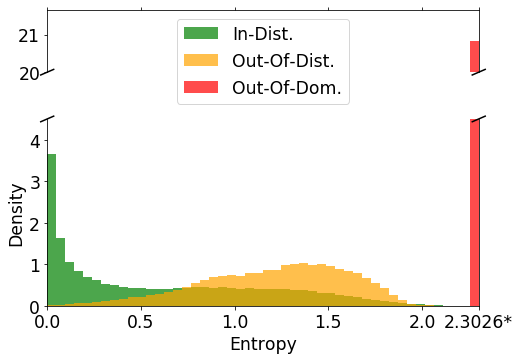
\includegraphics[width=.98 \textwidth]{sections/006_neurips2020/figures/entropy_CIFAR10.png}
        \caption{ID/OOD/OODom entropy}
    \end{subfigure}%  
    \begin{subfigure}[t]{0.33 \textwidth}
        \centering
        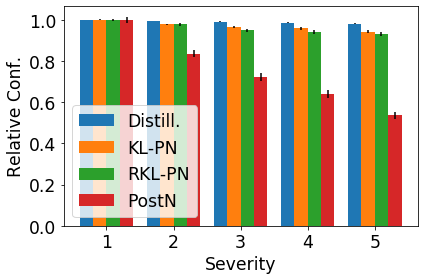
\includegraphics[width=.98 \textwidth]{sections/006_neurips2020/figures/shifts_CIFAR10_conf.png}
        \caption{Confidence under data shifts}
    \end{subfigure}%   
    \begin{subfigure}[t]{0.33 \textwidth}
        \centering
        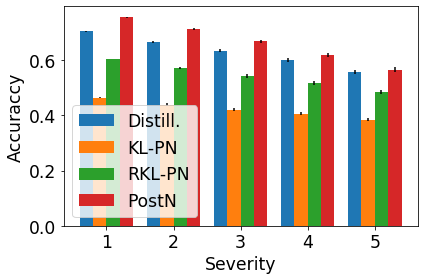
\includegraphics[width=.98 \textwidth]{sections/006_neurips2020/figures/shifts_CIFAR10_acc.png}
        \caption{Accuracy under data shifts}
    \end{subfigure}%   
    \caption{(a) shows entropy of the aleatoric distributions predicted by \PostNetacro on CIFAR10 (ID) and SVHN (OOD, OODom). The value $2.3026^*$ denotes the highest achievable entropy for 10 classes. \PostNetacro can easily distinguish between the three data types. (b) and (c) present averaged confidence and accuracy under 15 dataset shifts introduced by \cite{benchmarking-corruptions} on CIFAR10 with conv. architecture. On more severe perturbations (i.e. data further away from data distribution), \PostNetacro assigns higher epistemic uncertainty as desired. Baselines keeps same confidence even for less accurate predictions.}
    \label{cifar_shifts}
    %\vspace{-.5cm}
\end{figure}
\section{Conclusion}
\label{sec:conclusion_006}

We propose \ours, a model for uncertainty estimation in classification without requiring out-of-distribution samples for training or costly sampling for uncertainty estimation. \oursacro is composed of three main components: an encoder which outputs a position in a latent space, a normalizing flow which performs a density estimation in this latent space, and a Bayesian loss for uncertainty-aware training. In our extensive experimental evaluation, \oursacro achieves state-of-the-art performance with a strong improvement for detection of in- and out-of-distribution samples.

% \section*{Retrospective}
% \addcontentsline{toc}{section}{\protect Retrospective}%
\chapter{Uncertainty Estimation for Regression}
\label{chap:regression}

\section{Introduction}

\begin{wrapfigure}{r}{0.45\textwidth}
\vspace{-6mm}
	\centering
	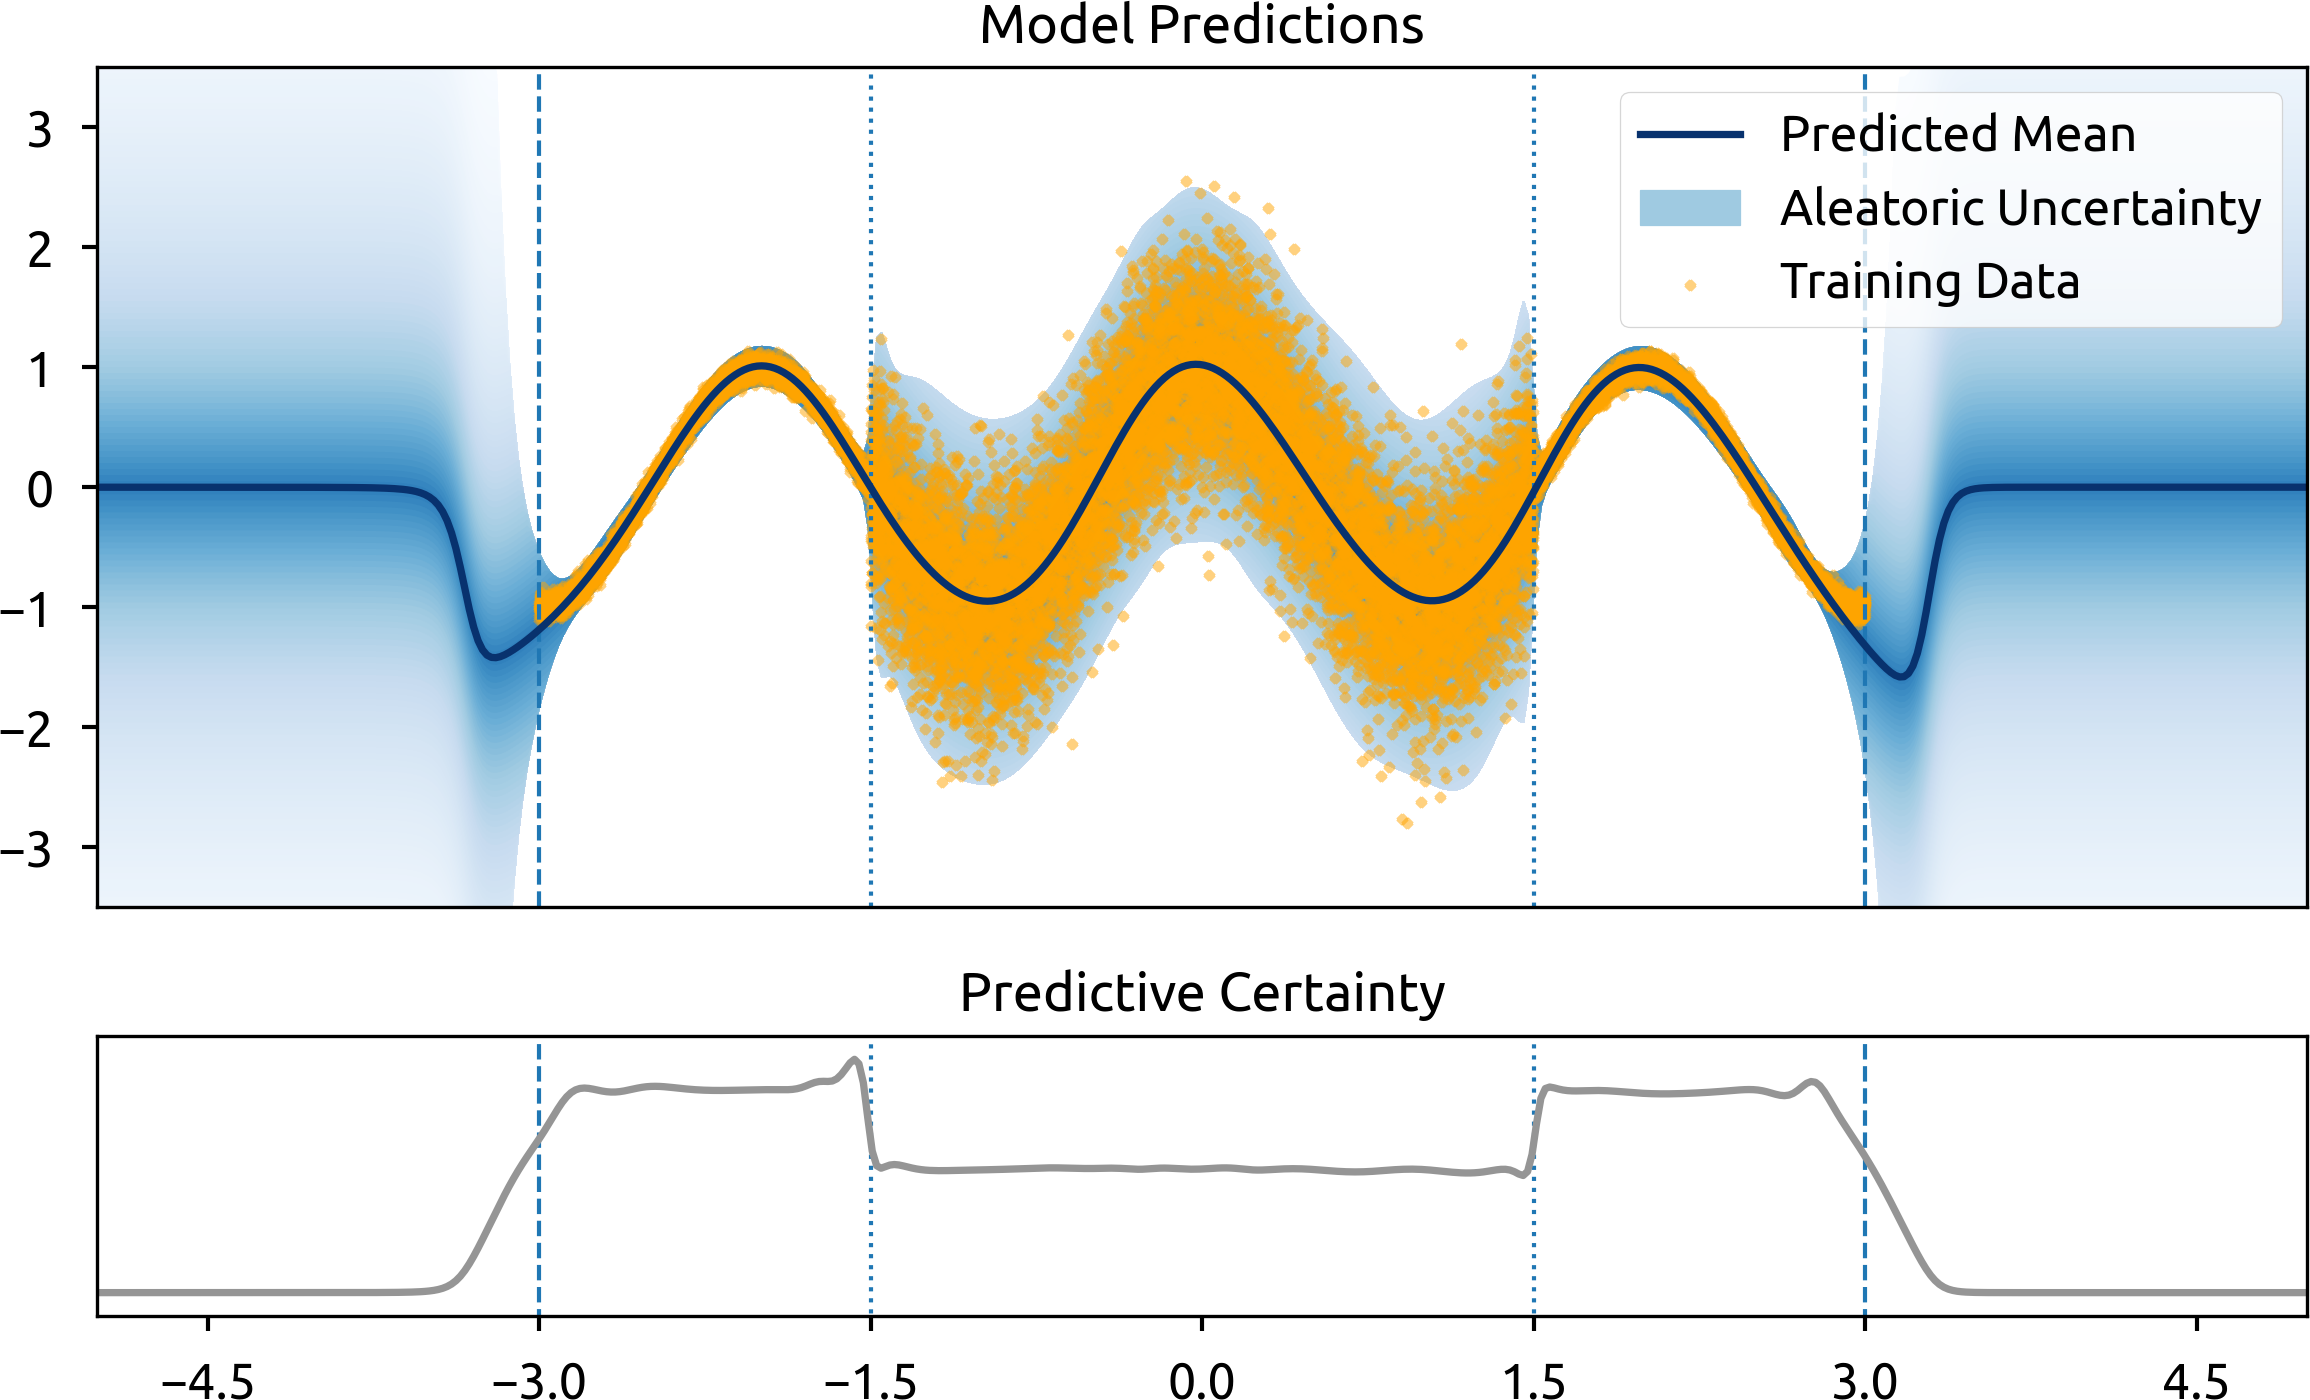
\includegraphics[width=0.42\textwidth]{sections/007_iclr2022/resources/toy-regression-trimmed.png}
    \caption*{Toy Regression Task}
    \vspace{0.3cm}
    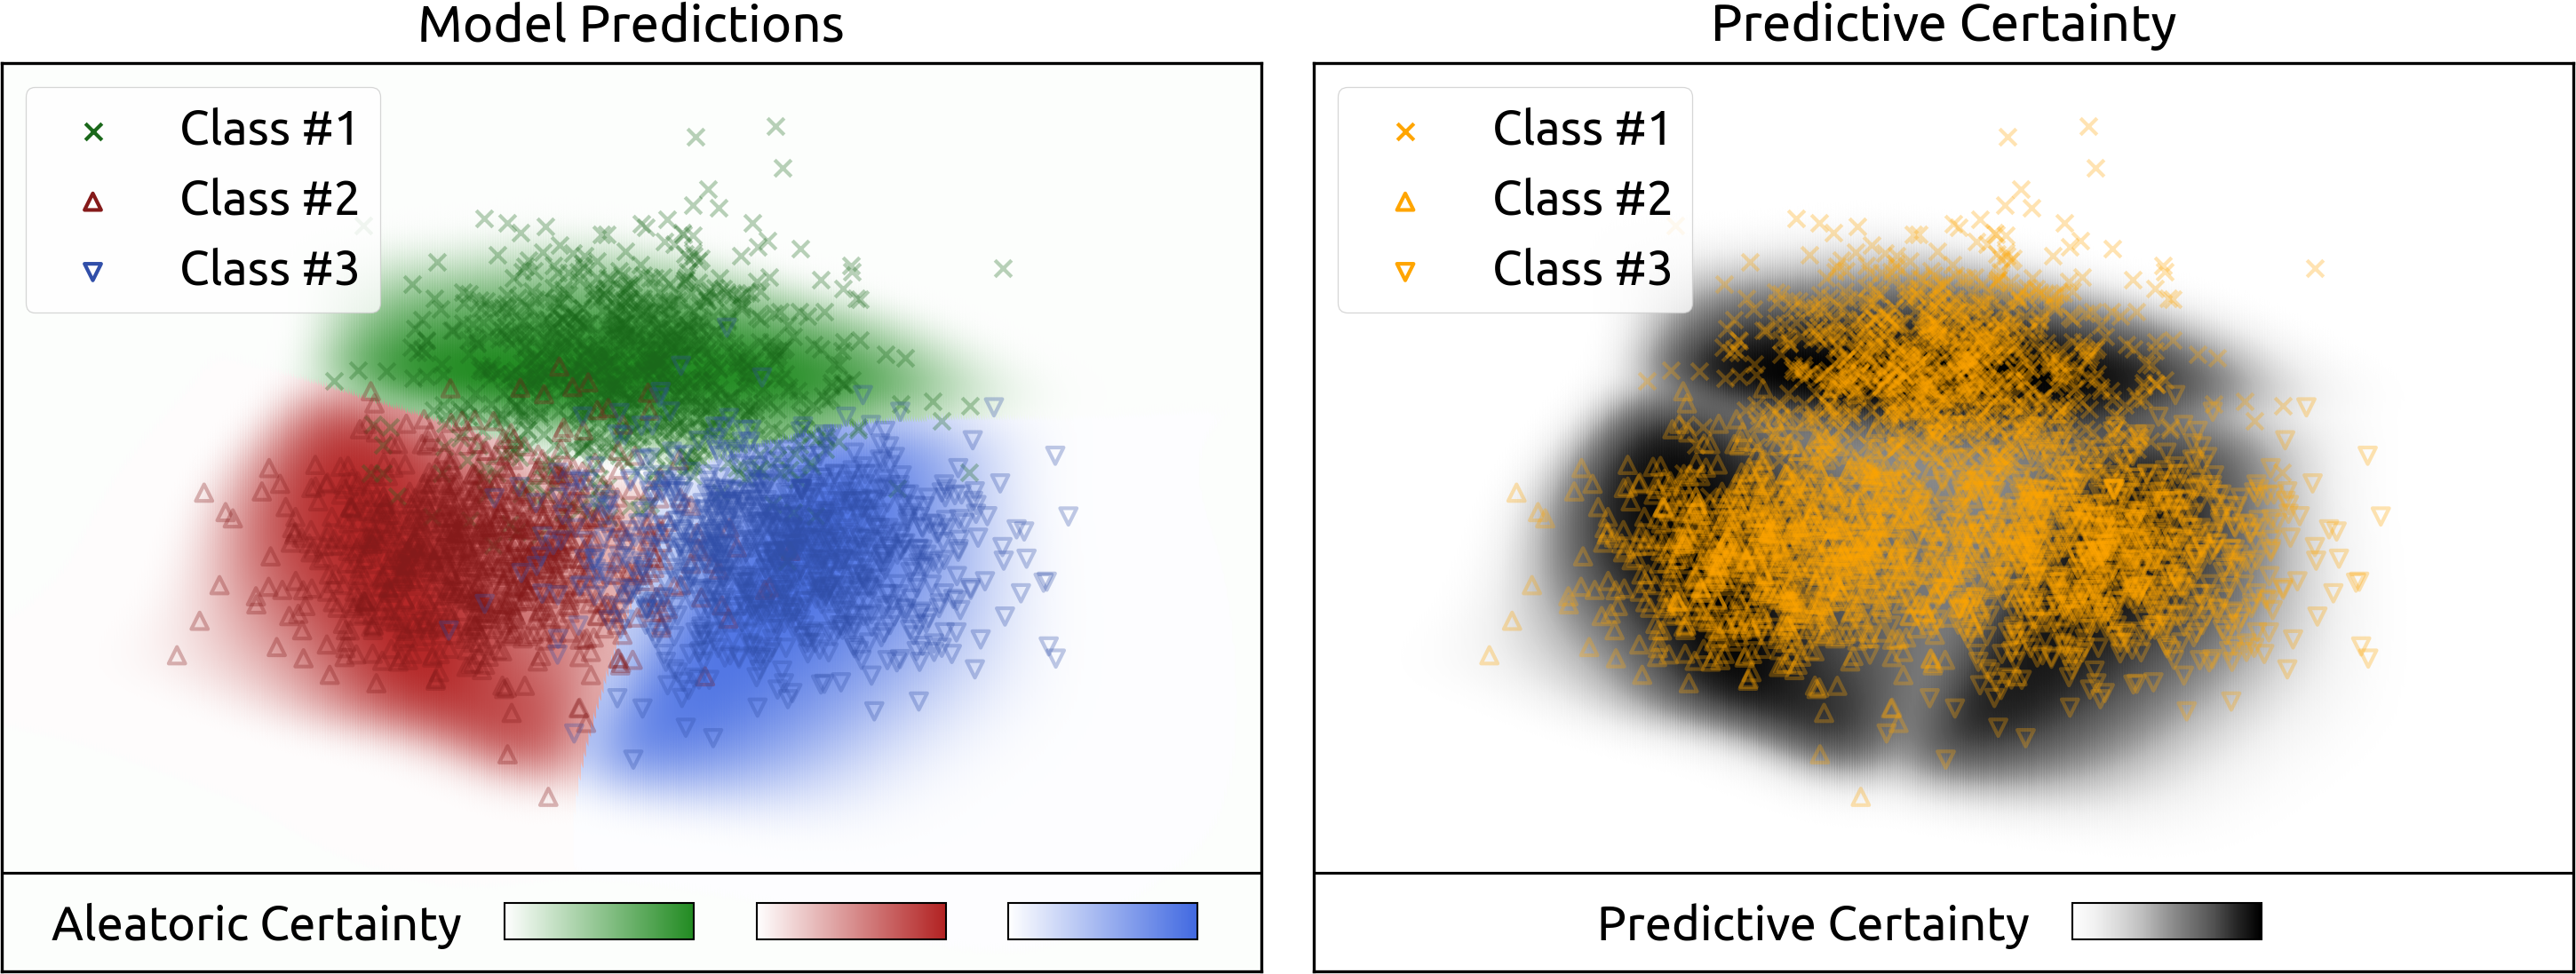
\includegraphics[width=0.42\textwidth]{sections/007_iclr2022/resources/toy-classification-trimmed.png}
    \caption*{Toy Classification Task}
    \caption{Visualization of the aleatoric and predictive uncertainty estimates of \NatPNacro{} on two toy regressions and classification tasks. \NatPNacro{} correctly assigns higher uncertainty to regions far from the training data.}
    \label{fig:toy-example-uncertainty}
    \vspace{-6mm}
\end{wrapfigure}

Accurate and rigorous uncertainty estimation is key for reliable machine learning models in safety-critical domains. It quantifies the confidence of machine learning models, thus allowing them to validate knowledgeable predictions corresponding to correct/wrong predictions, flag predictions on unknown input domains corresponding to anomaly or Out-of-Distribution detection, or detect natural shifts of the data facilitating real-time model maintenance \citep{dataset-shift, shifts-dataset, comparison-bayesian-diabetic}. Specifically, a reliable model can handle all these failure modes with high-quality estimates of \emph{aleatoric} and \emph{epistemic} uncertainty \citep{uncertainty-deep-learning}. These two levels of uncertainty allow a model to account for both irreducible data uncertainty (e.g. a fair dice's chance of $1/6$ for each face) and uncertainty due to the lack of knowledge about unseen data (e.g. input features differing significantly from training data or a covariate shift) respectively. Aleatoric and epistemic uncertainty levels can eventually be combined into an overall \emph{predictive uncertainty} \citep{uncertainty-deep-learning}

Traditional neural networks are not readily applicable in safety-critical domains as they show overconfident prediction, in particular on data that is different from training data \citep{calibration-network, ensembles}. To mitigate this problem, an important model family for uncertainty estimation directly predicts the parameters of a \emph{conjugate prior distribution} on the predicted \emph{target probability distribution}, thus accounting for the different levels of uncertainty. These models are efficient as they only require \emph{a single forward pass} for target and uncertainty prediction. Most of those models focus on classification and thus predict parameters of a Dirichlet distribution \citep{uceloss,postnet,priornet,reverse-kl,max_gap_id_ood,uncertainty-generative-classifier,multifaceted_uncertainty,graph_posterior,graph_uncertainty, lightweight-prob-net}. However, only two works \citep{evidential-regression, regression-priornet} have focused on regression by learning parameters of a Normal Inverse-Gamma (NIG) distribution as conjugate prior. Hence, all these models are limited to a \emph{single} task (e.g. either classification or regression). Some approaches even require out-of-distribution (OOD) data at training time \citep{priornet, reverse-kl} which is an unrealistic assumption in many real-world applications where anomalies are a priori diverse, rare or unknown.

\textbf{Our contribution.} We propose \NatPN{} (\NatPNacro{}) as a new approach parametrizing conjugate prior distributions for versatile uncertainty estimation. \NatPNacro{}{} is motivated from both the theoretical and practical perspective. 
\textbf{(1)} \NatPNacro{} can estimate predictive uncertainty for \emph{any} task described by the general group of exponential family distributions contrary to existing approaches from this family of models. Notably, this encompasses very common tasks such as classification, regression and count prediction which can be described with Categorical, Normal and Poisson distributions, respectively. 
\textbf{(2)} In theory, \NatPNacro{} is based on a \emph{new unified exponential family framework} which performs an input-dependent Bayesian update. For every input, it predicts the parameters of the posterior over the target exponential family distribution. We show that this Bayesian update is \emph{guaranteed} to predict high uncertainty far from training data.
\textbf{(3)} In practice, \NatPNacro{} requires \emph{no OOD data for training}, only adds \emph{a single normalizing flow} density to the last predictor layer and provides fast uncertainty estimation in a \emph{single forward pass}. Our extensive experiments showcase the high performances of \NatPNacro{} for various criteria (accuracy, calibration, OOD and shift detection) and tasks (classification, regression and count prediction). We illustrate the accurate aleatoric and predictive uncertainty predictions of \NatPNacro{} on two toy examples for classification and regression in Fig.~\ref{fig:toy-example-uncertainty}. \emph{None of the conjugate prior related works} have similar theoretical and practical properties.

%flexible, sound, simple, high quality, fast

\section{Related Work}
\label{sec:related_work_007}

In this section, we describe other work related to uncertainty estimation for supervised learning. We refer to \citet{uncertainty-survey} for a detailed survey on uncertainty estimation in deep learning. 

\textbf{Sampling-based methods.} A first family of models estimates uncertainty by aggregating statistics (e.g. mean and variance) from different samples of an implicit predictive distribution. Examples are ensemble \citep{bayesian-classifier-combination,ensembles, dynamic-bayesian-combination-classifiers,batch-ensembles,hyper-ensembles} and dropout \citep{dropout} models which provide high-quality uncertainty estimates \citep{dataset-shift} at the cost of an
expensive sampling phase at inference time. Moreover, ensembles usually require training multiple models. Further, Bayesian neural networks (BNN) \citep{bayesian-networks, scalable-laplace-bnn, simple-baseline-uncertainty} model the uncertainty on the weights and also require multiple samples to estimate the uncertainty on the final prediction. While recent BNNs have shown reasonably good performance \citep{rank-1-bnn,practical-bayesian,liberty-depth-bnn}, modelling the distribution on the weights suffers from pathological behavior thus limiting these approaches in practice \citep{expressiveness-bnn, practical-bnn, what-bnn-posterior}. In particular, \citet{what-bnn-posterior} uses an enormous computation budget by parallelizing the computation over 512 TPUv3  devices and running tens of thousands of training epochs to achieve a more exact Bayesian inference which is not suitable for practical applications. In contrast, \NatPNacro{} predicts uncertainty in \emph{a single forward pass} with a \emph{closed-form posterior distribution} over the target variable. \NatPNacro{} \emph{does not} model uncertainty on the weights.

\textbf{Sampling-free methods.} A second family of models is capable of estimating uncertainty in a single forward pass. The family of models parametrizing conjugate prior distributions is the main focus of this paper \citep{survey_evidential_uncertainty,evaluating_dbu,max_gap_id_ood,uncertainty-generative-classifier,multifaceted_uncertainty,graph_posterior, lightweight-prob-net}. Beyond this family of models, we differentiate between four other families of sampling-free models for uncertainty estimation. A first family aims at learning deep Gaussian processes with random features projections or learned inducing points \citep{uncertainty-distance-awareness, due, duq, uceloss}. A second family aims at learning deep energy-based models \citep{ood_ebm, jem_ebm}. Another family of models aims at propagating uncertainty across layers \citep{natural-parameter-network, sampling-free-variance-propagation, feed-forward-propagation, lightweight-prob-net, probabilistic-backprop-scalable-bnn}. They model uncertainty at the weight and/or activation levels and are generally constrained to specific transformations. In contrast, \NatPNacro{} only models the uncertainty on the predicted target variable and does not enforce any constraint on the encoder architecture. Further, some of the models propagating uncertainty already used the exponential family framework \citep{natural-parameter-network, deep-exponential-families}. However, while they parametrize exponential family distributions, \NatPNacro{} parametrizes the \emph{conjugate prior of the target exponential family distributions} which accounts for the epistemic uncertainty. Finally, while the family of calibration models aims at calibrating predictions \citep{accurate-uncertainties-deep-learning-regression, confidence-aware-learning, individual-calibration, distribution-calibration-regression, intra-order-preserving}, \NatPNacro{} aims at accurately modelling both aleatoric and epistemic uncertainty on in- and out-of-distribution data.

\section{Natural Posterior Network}
\label{sec:model_007}

At the very core of \NatPNacro{} stands the Bayesian update rule: $    \prior(\expparam \condition \mathcal{D}) \propto \prob(\mathcal{D} \condition \expparam) \times \prior(\expparam)$
%
%\begin{equation}\label{eq:general-bayesian-update}
%    \prior(\expparam \condition \mathcal{D}) \propto \prob(\mathcal{D} \condition \expparam) \times \prior(\expparam)
%\end{equation}
%
where $\prob(\mathcal{D} \condition \expparam)$ is the target distribution of the target data $\mathcal{D}$ given its parameter $\expparam$, and $\prior(\expparam )$ and $\prior(\expparam \condition \mathcal{D})$ are the prior and posterior distributions, respectively, over the target distribution parameters. The target distribution $\prob(\mathcal{D} \condition \expparam)$ could be any likelihood describing the observed target labels. The Bayesian update has three main advantages: \textbf{(1)} it introduces a prior belief which represents the safe default prediction if no data is observed, \textbf{(2)} it updates the prior prediction based on observed target labels, and \textbf{(3)} it assigns a confidence for the new target prediction given the aggregated evidence count of observed target labels. While \NatPNacro{} is capable to perform a Bayesian update for every possible input given the observed training data, we first recall the Bayesian background for a single exponential family distribution.

\begin{table*}[ht!]
	\vspace{-3mm}
	\centering
	\resizebox{.89\textwidth}{!}{%
\begin{tabular}{lccl}
\toprule
\multicolumn{1}{c}{Likelihood $\prob$} & \multicolumn{1}{c}{Conjugate Prior $\prior$} & \multicolumn{1}{c}{Parametrization Mapping $m$} & \multicolumn{1}{c}{Bayesian Loss (Eq.~\ref{eq:bayesian-loss})}\\
\midrule
\midrule
$\y \sim \DCat(\bm{p})$ & 
$\bm{p} \sim \DDir(\bm{\alpha})$ & 
\begin{tabular}{@{}l@{}}
$\priorparam=\bm{\alpha}/\evidence$ \\
$\evidence=\sum_\iclass \alpha_\iclass$
\end{tabular} &
\begin{tabular}{@{}l@{}}
    \textbf{(i)} $= \psi(\alpha_{\y*}\dataix) - \psi(\alpha_0\dataix)$ \\
    \textbf{(ii)} $= \log B(\bm{\alpha}\dataix) + (\alpha_0\dataix - \nclass) \psi(\alpha_0\dataix) - \sum_\iclass (\alpha_\iclass\dataix - 1) \psi(\alpha_\iclass\dataix)$
\end{tabular} \\
\midrule
$\y \sim \DNormal(\mu, \sigma)$ & 
$\mu, \sigma \sim \DNIG(\mu_0, \lambda, \alpha, \beta)$ & 
\begin{tabular}{@{}l@{}}
$\priorparam=\begin{pmatrix}\mu_0 \\ \mu_0^2 + \frac{2\beta}{\evidence} \end{pmatrix}$\\
$\evidence = \lambda= 2 \alpha$
\end{tabular} &
\begin{tabular}{@{}l@{}}
    \textbf{(i)} $= \frac{1}{2}\left(- \frac{\alpha}{\beta} (\y - \mu_0)^2 - \frac{1}{\lambda} + \psi(\alpha) - \log{\beta} - \log{2\pi}\right)$ \\
    \textbf{(ii)} $= \frac{1}{2} + \log\left((2\pi)^{\frac{1}{2}}\beta^{\frac{3}{2}}\Gamma(\alpha)\right) - \frac{1}{2} \log{\lambda} + \alpha - (\alpha+\frac{3}{2})\psi(\alpha)$
\end{tabular}\\
\midrule
$\y \sim \DPoi(\lambda)$ &
$\lambda \sim \DGamma(\alpha, \beta)$ &
\begin{tabular}{@{}l@{}}
$\chi=\alpha/\evidence$ \\
$\evidence=\beta$
\end{tabular} &
\begin{tabular}{@{}l@{}}
    \textbf{(i)} $= (\psi(\alpha) - \log{\beta}) \y - \frac{\alpha}{\beta} - \sum_{k=1}^{\y} \log k$ \\
    \textbf{(ii)} $= \alpha + \log{\Gamma(\alpha)} - \log{\beta} + (1 - \alpha) \psi(\alpha)$
\end{tabular}\\
\bottomrule
\end{tabular}}
	\caption{Examples of Exponential Family Distributions where $\psi(x)$ and $B(x)$ denote Digamma and Beta function, respectively.}
	\label{tab:summary_exp_dist}
	\vspace{-3mm}
\end{table*}

\subsection{Exponential Family Distribution}
% \textbf{Exponential Family Distribution.} 
Distributions from the exponential family are very widely used and have favorable analytical properties. Indeed, \textbf{(1)} they cover a wide range of target variables like discrete, continuous, counts or spherical coordinates, and \textbf{(2)} they benefit from intuitive and generic formulae for their parameters, density functions and statistics which can often be evaluated in closed-form. Important examples of exponential family distributions are Normal, Categorical and Poisson distributions (see Tab.~\ref{tab:summary_exp_dist}). Formally, an exponential family distribution on a target variable $\y \in \real$ with \emph{natural parameters} $\expparam \in \real^\suffstatdim$ can be denoted as
%
\begin{equation}\label{eq:exponential-family}
    \prob(\y \condition \expparam) = h(\y) \exp\left(\expparam^T \bm{u}(\y) - A(\expparam)\right)
\end{equation}
%
where ${h: \real \rightarrow \real}$ is the \emph{carrier or base measure}, ${A: \real^\suffstatdim \rightarrow \real}$ the \emph{log-normalizer} and ${\bm{u}: \real \rightarrow \real^\suffstatdim}$ the \emph{sufficient statistics} \citep{bishop,exponential-entropy}. The entropy of an exponential family distribution can always be written as $\entropy[\prob] = A(\expparam) - \expparam^T \nabla_{\bm{\theta}}A(\expparam) - \expectation[\log{h(\y)}]$ \citep{exponential-entropy}.
An exponential family distribution always admits a conjugate prior, which often also is a member of the exponential family:
%
\begin{equation}\label{eq:prior}
    \prior(\expparam \condition \priorparam, \evidence) = \eta(\priorparam, \evidence) \exp\left( \evidence \, \bm{\theta}^T\priorparam  - \evidence A(\expparam) \right)
\end{equation}
%
where $\eta(\priorparam, \evidence)$ is a normalization coefficient, $\priorparam \in \real^L$ are \emph{prior parameters} and $\evidence \in \real^+$ is the \emph{evidence}. Given a set of $\ndata$ target observations $\{\y^{(i)}\}_{i}^{\ndata}$, it is easy to compute a closed-form Bayesian update $\prior(\expparam \condition \priorparam^\text{post}, \evidence^\text{post}) \propto \prob(\{\y^{(i)}\}_{i}^{\ndata} \condition \expparam) \times \prior(\expparam \condition \chi^\text{prior}, n^\text{prior})$:
%
\begin{equation}\label{eq:posterior}
    \prior(\expparam \condition \priorparam^\text{post}, \evidence^\text{post}) \propto \exp\left( \evidence^\text{post} \expparam^T\priorparam^\text{post} - \evidence^\text{post} A(\expparam) \right)
\end{equation}
%
where $\priorparam^\text{post}=\frac{\evidence^\text{prior} \priorparam^\text{prior}+ \sum_{j}^\ndata{\bm{u}(\y^{(j)})}}{\evidence^\text{prior} + \ndata}$ and $\evidence^\text{post}=\evidence^\text{prior} + \ndata$. We see that $\priorparam^{\text{prior}}$ (resp. $\priorparam^{\text{post}}$) can be viewed as the average sufficient statistics of $\evidence^{\text{prior}}$ (resp. $\evidence^{\text{post}}$) fictitious samples \citep{bishop}. 
Further, the average sufficient statistic of fictitious samples is equal to the expected sufficient statistic of the conjugate distribution, i.e. $\priorparam = \expectation_{\prior(\priorparam, \evidence)}[\expparam]$ \citep{exponential-family-stats, conjugate-prior-exponential-family}. Thus, the parameter $\priorparam^\text{post}$ carries the inherent aleatoric uncertainty on the target distribution with natural parameters $\expparam$, while the evidence $\evidence^\text{post}$ aligns well with the epistemic uncertainty (i.e. a low evidence means few prior target observations). We stress that the natural conjugate prior parametrization $\priorparam, \evidence$ is often different from the ``well-known'' parametrization $\bm{\kappa}$ used by standard coding libraries. By definition, a bijective mapping $m(\bm{\kappa}) = (\priorparam, \evidence)$ from the natural parametrization to the commonly used parametrization always exists (see examples in Tab.~\ref{tab:summary_exp_dist}). Finally, exponential family distributions always admit a closed-form posterior predictive distribution \citep{bayesian-data-analysis}.

\subsection{Input-Dependent Bayesian Update for Exponential Family Distributions}
%\textbf{Input-Dependent Bayesian Update for Exponential Family Distributions.} 
We propose to leverage the power of exponential family distributions for the more complex task when the prediction $\y\dataix$  depends on the input $\x\dataix$. Hence, \NatPNacro{} extends the Bayesian treatment of a single exponential family distribution prediction by predicting an individual posterior update per input. We distinguish between the chosen prior parameters $\priorparam^\text{prior}$, $\evidence^\text{prior}$ shared among samples, and the additional predicted parameters $\priorparam\dataix$, $\evidence\dataix$ dependent on the input $\x\dataix$ leading to the updated posterior parameters:
%
\begin{equation}\label{eq:parameter-update}
    \priorparam^{\text{post},(\idata)} = \frac{\evidence^\text{prior}\priorparam^\text{prior} + \evidence\dataix \priorparam\dataix}{\evidence^\text{prior} + \evidence\dataix}, \hspace{5mm}
    \evidence^{\text{post},(\idata)} = \evidence^\text{prior} + \evidence\dataix
\end{equation}
%
Equivalently, \NatPNacro{} may be interpreted as predicting a set of $\evidence\dataix$ pseudo observations $\{\y^{(j)}\}_{j}\dataix$ such that their aggregated sufficient statistics satisfy \smash{$\sum_{j}^{\evidence\dataix} \y^{(j)} = \evidence\dataix \priorparam\dataix$}, and perform the respective Bayesian update.
%
% \begin{equation}\label{eq:bayesian-update}
%     \begin{aligned}
% \prior(\expparam \condition \{\y^{(j)}\}_{j}\dataix) \propto \prob(\{\y^{(j)}\}_{j}\dataix \condition \expparam) \times \prior(\expparam)
%     \end{aligned}
% \end{equation}
%
This Bayesian update works for \emph{any} choice of exponential family distributions as long as parameters are mapped to their standard form (see Tab.~\ref{tab:summary_exp_dist}). According to the \emph{principle of maximum entropy} \citep{maximum-entropy-principle}, a practical choice for the prior is to enforce high entropy for the prior distribution which is usually considered less informative. It is typically achieved when the prior pseudo-count $\evidence^\text{prior}$ is small and the prior parameter $\priorparam^\text{prior}$ shows a high aleatoric uncertainty.

\begin{figure*}[t]
    \centering
    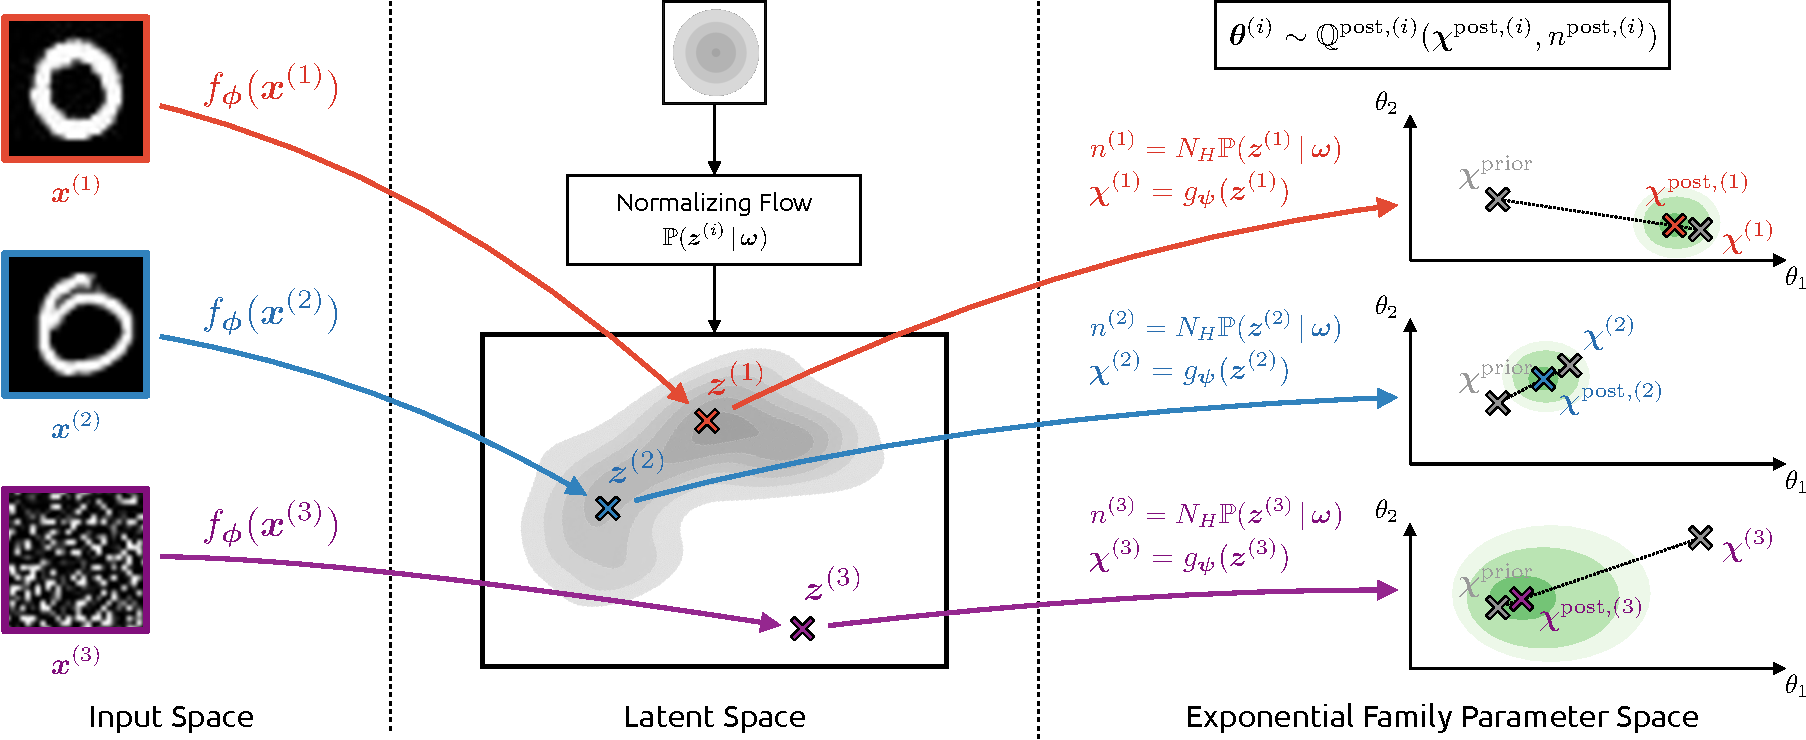
\includegraphics[width=.85\linewidth]{sections/007_iclr2022/resources/npn-crop.pdf}
    \caption{Overview of \NatPN{}. Inputs $\bm{x}^{(i)}$ are first mapped to a low-dimensional latent representation $\bm{z}^{(i)}$ by the encoder $f_{\bm{\phi}}$. From $\bm{z}^{(i)}$, the decoder $g_{\bm{\psi}}$ derives the parameter update $\bm{\chi}^{(i)}$ while a normalizing flow $\mathbb{P}_{\bm{\omega}}$ yields the evidence update $n^{(i)}$. Posterior parameters are obtained from a weighted combination of prior and update parameters according to $n^{\text{post},(i)}$.}
    \label{fig:npn}
    % \vspace{-1mm}
\end{figure*}

Hence, \NatPNacro{} proposes a generic way to perform the input-dependent Bayesian update $\priorparam\dataix$, $\evidence\dataix$ for \emph{any} exponential family distribution in three steps (see Fig.~\ref{fig:npn}): \textbf{(1)} An encoder $f_{\bm{\phi}}$ maps the input $\x\dataix$ onto a low-dimensional latent vector $\z\dataix = f_{\phi}(\x\dataix) \in \real^H$ representing useful features for the prediction task (see left Fig.\ref{fig:npn}). Note that the architecture of the encoder can be arbitrarily complex. Then, \textbf{(2)} the latent representation $\z\dataix$ is used in two different ways to predict the parameter update $\priorparam\dataix$ and the evidence update $\evidence\dataix$ (see center Fig.\ref{fig:npn}). On the one hand, a linear decoder $g_{\bm{\psi}}$ is trained to output the parameter update $\priorparam\dataix = g_{\bm{\psi}}(\z\dataix) \in \real^L$ accounting for the aleatoric uncertainty. On the other hand, a single normalized density is trained to output the evidence update $\evidence\dataix = N_H\prob(\z\dataix \condition \bm{\omega})$ accounting for the epistemic uncertainty. The intuition is that increasing the evidence on training data during training forces the evidence everywhere else (incl. far from training data) to decrease thanks to the density normalization constraint. The constant $N_H$ is a certainty budget distributed by the normalized density $\prob(\z\dataix \condition \bm{\omega})$ over the latent representations $\z\dataix$ i.e. $N_H = \int N_H \prob(\z\dataix \condition \bm{\omega}) d\z\dataix = \int \evidence\dataix d\z\dataix$. In practice, we observed that scaling the certainty budget w.r.t. the latent dimension $H$ helped the density to cover larger volumes in higher dimension (see app.). Finally, \textbf{(3)} \NatPNacro{} computes the posterior parameters $\priorparam^{\text{post}, (\idata)}$ and $\evidence^{\text{post}, (\idata)}$ which can be viewed respectively as the mean and concentration of the posterior distribution (see right Fig.\ref{fig:npn}). Note that the posterior parameter $\priorparam^{\text{post}, (\idata)}$ is a simple weighted average of the prior parameter $\priorparam^\text{prior}$ and the update parameter $\priorparam\dataix$ as shown by Eq.~\ref{eq:parameter-update}.

\NatPNacro{} extends PostNet \citep{postnet} which also performs an input-dependent Bayesian update with density estimation. Yet, it has three crucial differences which lead to major practical improvements. First, the new exponential family framework is significantly more flexible and is not restricted to classification. Second, the Dirichlet $\bm{\alpha}$ parameter computation is different: \NatPNacro{} computes the $\priorparam$ parameters -- which can be viewed as standard softmax output -- and the $\evidence$ evidence separately (i.e. $\bm{\alpha} = \evidence \priorparam$) while PostNet computes one evidence pseudo-count per class. Third, \NatPNacro{} is computationally more efficient. It requires a single density while PostNet requires $\nclass$ densities.

\subsection{ID and OOD Uncertainty Estimates}
%\textbf{ID and OOD Uncertainty Estimates.} 
\NatPNacro{} intuitively leads to reasonable uncertainty estimation for the two limit cases of strong in-distribution (ID) and out-of-distribution (OOD) inputs (see red and purple samples in Fig.~\ref{fig:npn}). For very likely \emph{in-distribution} data (i.e. $\prob(\z\dataix \condition \bm{\omega}) \rightarrow \infty$), the posterior parameter overrules the prior (i.e. $\priorparam^{\text{post}, (\idata)} \rightarrow \priorparam\dataix$). Conversely, for very unlikely \emph{out-of-distribution} data (i.e. $\prob(\z\dataix \condition \bm{\omega}) \rightarrow 0$), the prior parameter takes over in the posterior update (i.e. $\priorparam^{\text{post}, (\idata)} \rightarrow \priorparam^\text{prior}$). Hence, the choice of the prior parameter should reflect the default prediction when the model lacks knowledge. We formally show under mild assumptions on the encoder that \NatPNacro{} predicts very low additional evidence ($\evidence\dataix \approx 0$) for (almost) any input $\x\dataix$ far away from the training data (i.e. $||\x\dataix|| \rightarrow + \infty$), thus recovering prior predictions (i.e. $\priorparam^{\text{post}, (\idata)} \approx \priorparam^\text{prior}$) (see proof in app.).
\begin{theorem}
\label{thm:oodom-guarantee}
Let a \NatPNacro{} model be parametrized with a (deep) encoder $f_{\phi}$ with ReLU activations, a decoder $g_{\psi}$ and the density $\prob(\z \condition \bm{\omega})$. Let $f_{\phi}(\x)= V^{(l)}\x + a^{(l)}$ be the piecewise affine representation of the ReLU network $f_{\phi}$ on the finite number of affine regions $Q^{(l)}$ \citep{understanding-nn-relu}. Suppose that $V^{(l)}$ have independent rows and the density function $\prob(\z \condition \bm{\omega})$ has bounded derivatives, then for almost any $\x$ we have \smash{$\prob(f_{\phi}(\delta \cdot \x) \condition \bm{\omega}) \underset{\delta \rightarrow \infty}{\rightarrow} 0$}. i.e the evidence becomes small far from training data.
\end{theorem}
This theorem only requires that the density avoids very unlikely pathological behavior with unbounded derivatives \citep{limit-existence-infinity}. A slightly weaker conclusion holds using the notion of limit in density if the density function does not have bounded derivatives \citep{integrable-infinity}. Finally, the independent rows condition is realistic for trained networks with no constant output \citep{overconfident-relu}. It advantageously leads \NatPNacro{} to consistent uncertainty estimation contrary to standard ReLU networks which are overconfident far from training data \citep{overconfident-relu}.

\subsection{Bayesian \NatPNacro{} Ensemble} 
%\textbf{Bayesian \NatPNacro{} Ensemble.} 
Interestingly, it is natural to extend the Bayesian treatment of a single \NatPNacro{} to an ensemble of \NatPNacro{} models (NatPE). An ensemble of $m$ \NatPNacro{} models is intuitively equivalent to performing $m$ successive Bayesian updates using each \NatPNacro{} member separately. More formally, given an input $\x\dataix$ and an ensemble of $m$ jointly trained \NatPNacro{} models, the Bayesian update for the posterior distribution becomes ${\priorparam^{\text{post}, (\idata)} = \frac{\evidence^\text{prior}\priorparam^\text{prior} + \sum_k^{m} \evidence_k\dataix \priorparam_k\dataix}{\evidence^\text{prior} + \sum_k^{m} \evidence_k\dataix}}$ and ${\evidence^{\text{post}, (\idata)} = \evidence^\text{prior} + \sum_k^{m} \evidence_k\dataix}$. %which is equivalent to having observed $m$ sets of \smash{$\evidence_k\dataix$} pseudo observations. %$\{\y_k^{(j)}\}_{j}\dataix$ such that $\sum_{j}^{\evidence_m\dataix} \y^{(j)} = \priorparam_k\dataix$. 
Note that the standard Bayesian averaging which is used in many ensembling methods \citep{bayesian-ensemble-learning,ensembles,batch-ensembles,hyper-ensembles} is different from this Bayesian combination. While Bayesian averaging assume that only one model is correct, the Bayesian combination of \NatPNacro{} allows \emph{more} or \emph{none} of the models to be ``expert'' for some input  \citep{bayesian-averaging-to-combination}. For example, an input $\x\dataix$ unfamiliar to every model $m$ (i.e. $\evidence_m\dataix \approx 0$) would recover the prior default prediction $\priorparam^\text{prior}, \evidence^\text{prior}$. Existing models already had similar properties for Bayesian combination of classifiers \citep{bayesian-classifier-combination, dynamic-bayesian-combination-classifiers}.

\subsection{Optimization}
\label{sec:optimization}

The choice of the optimization procedure is of primary importance in order to obtain both high-quality target predictions and uncertainty estimates regardless of the task.

\paragraph{Bayesian Loss.} We follow \cite{postnet} and aim at minimizing the Bayesian formulation:
%
\begin{equation}\label{eq:bayesian-loss}
    \mathcal{L}\dataix = - \underbrace{\expectation_{\expparam\dataix \sim \prior^{\text{post},(\idata)}}[\log \prob(\y\dataix\condition \expparam \dataix)]}_\text{(i)} - \underbrace{\entropy[\prior^{\text{post},(\idata)}]}_\text{(ii)}
\end{equation}
%
where $\entropy[\prior^{\text{post},(\idata)}]$ denotes the entropy of the predicted posterior distribution $\prior^{\text{post},(\idata)}$. Similarly to the ELBO loss, this loss is guaranteed to be optimal when the predicted posterior distribution is close to the true posterior distribution $\prior^*(\expparam \condition \x\dataix)$ i.e. $\prior^{\text{post},(\idata)} \approx \prior^*(\expparam \condition \x\dataix)$ \citep{update-belief-propagation, PAC-bayesian_estimator, opt-info-processing_bayes}. However, this loss is generally \emph{not} equal to the ELBO loss especially for real valued targets i.e. $y \in \real$ (see app.). The term \textbf{(i)} is the expected likelihood under the predicted posterior distribution. It can be viewed as the Uncertain Cross Entropy (UCE) loss \citep{uceloss} which is known to reduce uncertainty on observed data. The term \textbf{(ii)} is an entropy regularizer acting as a prior which favors uninformative distributions $\prior^{\text{post},(\idata)}$ with high entropy. In our case, we assume the likelihood $\prob(\y\dataix\condition\expparam\dataix)$ and the posterior $\prior^{\text{post},(\idata)}$ to be members of the exponential family. We take advantage of the convenient computations for such distributions and derive a more explicit formula for the Bayesian formulation \eqref{eq:bayesian-loss} (see derivation in the appendix):
%
\begin{equation}\label{eq:nll-entropy}
    \begin{aligned}
    \mathcal{L}_\lambda\dataix &\propto \expectation[\expparam]^T \bm{u}(y\dataix) - \expectation[A(\bm{\expparam})] - \lambda\entropy[\prior^{\text{post},(\idata)}]
    \end{aligned}
\end{equation}
%
where $\lambda$ is an additional regularization weight tuned with a grid search. Note that the term $\expectation[\expparam]^T \bm{u}(y\dataix) $ favors a good alignment of the expected sufficient statistic $\expectation[\expparam] = \priorparam$ with the observed sufficient statistic $\bm{u}(y\dataix)$. In practice, all terms can be computed efficiently in closed form for most exponential family distributions (see examples in Tab.~\ref{tab:summary_exp_dist}). In particular, simplifications are possible when the conjugate prior distribution is also in an exponential family which is often the case. Ultimately Eq.~\eqref{eq:nll-entropy} applies to \emph{any} exponential family distribution unlike \cite{postnet}.

\textbf{Optimization Scheme.} \NatPNacro{} is fully differentiable using the closed-form Bayesian loss. Thus, we train the encoder $f_{\bm{\phi}}$, the parameter decoder $g_{\bm{\psi}}$ and the normalizing flow $\prob(\z\dataix \condition \bm{\omega})$ w.r.t. parameters $\bm{\phi}, \bm{\psi}, \bm{\omega}$ jointly. Further, we observed that ``warm-up training'' \citep{warm-start} and ``fine-tuning'' \citep{fine-tuning-continuous} of the density helped to improve uncertainty estimation for more complex flows and datasets. Thus, we train the normalizing flow density to maximize the likelihood of the latent representations before and after the joint optimization while keeping all other parameters fixed.

\subsection{Model Limitations} \label{sec:limitations}

\paragraph{Task-Specific OOD.} Previous works show that density estimation is unsuitable for acting on the raw image input \citep{anomaly-detection,deep-generative,typicality_OOD_generative} or on a non-carefully transformed space \citep{perfect-density-no-ood-guarantee}. To circumvent this issue, \NatPNacro{} does not perform OOD detection directly on the input but rather fits a normalizing flow on a learned space. In particular, the latent space is \textbf{(1)} low-dimensional, \textbf{(2)} task-specific and \textbf{(3)} encodes meaningful semantic features. Similarly, \cite{postnet, why-nf-fail-ood, density-states-ood, contrastive-ood} already improved OOD detection of density-based methods by leveraging a task-induced bias or low-dimensional statistics. In the case of \NatPNacro{}, the low-dimensional latent space has to contain relevant features to linearly predict the sufficient statistics required for the task. For example, \NatPNacro{} aims at a linearly separable latent space for classification. The downside is that \NatPNacro{} is capable of detecting OOD samples only with respect to the considered task and requires labeled examples during training. As an example, \NatPNacro{} likely fails to detect a change of image color if the task aims at classifying object shapes and the latent space has no notion of color. Hence, we underline that \NatPNacro{} comes with a task-dependent OOD definition, which is a reasonable choice in practice.

\paragraph{Model-Task Mismatch.} Second, we emphasize that the uncertainty estimation quality of \NatPNacro{} for (close to) ID data depends on the convergence of the model, the encoder architecture (e.g. MLP, Conv., DenseDepth \citep{dense-depth}) and the target distribution (e.g. Poisson, Normal distributions) choice which should match the task needs. However, we show \emph{empirically} that \NatPNacro{} provides high quality uncertainty estimates in practice on a wide range of tasks. Further, we show \emph{theoretically} that \NatPNacro{} leads to uncertain prediction far away from training data for \emph{any} exponential family target distributions. In comparison, \cite{provable-uncertainty} showed akin guarantees for classification only.
\section{Experiments}
\label{sec:experiments_007}

In this section, we compare \NatPNacro{} to existing methods on extensive experiments including three different tasks: classification, regression and count prediction. For each task type, we evaluate the prediction quality based on target error and uncertainty metrics. These various set-ups aim to highlight the versatility of \NatPNacro{}. In particular, \NatPNacro{} is the only model that adapts to all tasks and achieves high performances for all metrics without requiring multiple forward passes.

\begin{table*}[ht]
    \centering
    % \vspace{-1mm}
   % \scriptsize
   \caption{Classification results on Sensorless Drive with Categorical target distribution. Best scores among all single-pass models are in bold. Best scores among all models are starred.}
    \label{tab:sensorless-drive}
    % \vspace{-3mm}
    \resizebox{0.8 \textwidth}{!}{
    \begin{tabular}{lcccccc}
        \toprule
        & \textbf{Accuracy} & \textbf{Brier} & \textbf{9/10 Alea.} & \textbf{9/10 Epist.} & \textbf{OODom Alea.} & \textbf{OODom Epist.} \\
        \midrule
        \textbf{Dropout} & 98.62 $\pm$ 0.11 & 3.79 $\pm$ 0.29 & 30.20 $\pm$ 0.85 & 32.57 $\pm$ 1.45 & 27.03 $\pm$ 0.51 & 95.30 $\pm$ 1.66 \\
        \textbf{Ensemble} & 98.83 $\pm$ 0.17 & 3.00 $\pm$ 0.54 & 30.79 $\pm$ 0.74 & 32.61 $\pm$ 1.06 & 27.16 $\pm$ 0.59 & 99.97 $\pm$ 0.01 \\
        \textbf{NatPE} & *99.66 $\pm$ 0.03 & *0.68 $\pm$ 0.05 & 77.05 $\pm$ 1.93 & 83.73 $\pm$ 1.89 & 99.99 $\pm$ 0.00 & *100.00 $\pm$ 0.00 \\
        \midrule
        \textbf{R-PriorNet} & 98.85 $\pm$ 0.25 & 2.01 $\pm$ 0.47 & 40.13 $\pm$ 2.99 & 30.07 $\pm$ 0.81 & \textbf{*100.00 $\pm$ 0.00} & 23.59 $\pm$ 0.00 \\
        \textbf{EnD$^2$} & 93.95 $\pm$ 2.35 & 28.09 $\pm$ 6.40 & 26.35 $\pm$ 0.60 & 24.85 $\pm$ 0.43 & 84.43 $\pm$ 15.21 & 23.58 $\pm$ 0.00 \\
        \textbf{PostNet} & \textbf{99.64 $\pm$ 0.02} & \textbf{0.75 $\pm$ 0.08} & 80.60 $\pm$ 1.68 & \textbf{*92.57 $\pm$ 1.41} & \textbf{*100.00 $\pm$ 0.00} & \textbf{*100.00 $\pm$ 0.00} \\
        \textbf{\NatPNacro{}} & 99.61 $\pm$ 0.05 & 1.04 $\pm$ 0.29 & \textbf{*81.43 $\pm$ 1.89} & 79.54 $\pm$ 2.62 & 99.98 $\pm$ 0.00 & \textbf{*100.00 $\pm$ 0.00} \\
        \bottomrule
    \end{tabular}
    }
            % \vspace{-0mm}
\end{table*}

%\begin{table*}[ht]
%    \centering
%    \scriptsize
%    \resizebox{1.\textwidth}{!}{
%    \begin{tabular}{lcccccccc}
%        \toprule
%        & \textbf{Accuracy} & \textbf{Brier} & \textbf{K. Alea.} & \textbf{K. Epist.} & \textbf{F. Alea.} & \textbf{F. Epist.} & \textbf{OODom Alea.} & \textbf{OODom Epist.} \\
%        \midrule
%        \textbf{Dropout} & 99.45 $\pm$ 0.01 & 1.07 $\pm$ 0.05 & 98.27 $\pm$ 0.05 & 97.82 $\pm$ 0.08 & *99.40 $\pm$ 0.03 & 98.01 $\pm$ 0.14 & 43.86 $\pm$ 1.62 & 74.09 $\pm$ 0.92 \\
%        \textbf{Ensemble} & 99.46 $\pm$ 0.02 & 1.02 $\pm$ 0.02 & 98.39 $\pm$ 0.07 & 98.43 $\pm$ 0.05 & 99.33 $\pm$ 0.06 & 98.73 $\pm$ 0.08 & 40.98 $\pm$ 1.80 & 66.54 $\pm$ 0.58 \\
%        \textbf{NatPE} & *99.55 $\pm$ 0.01 & *0.84 $\pm$ 0.03 & 96.39 $\pm$ 0.73 & *99.61 $\pm$ 0.02 & 97.49 $\pm$ 0.85 & *99.70 $\pm$ 0.04 & *100.00 $\pm$ 0.00 & *100.00 $\pm$ 0.00 \\
%        \midrule
%        \textbf{R-PriorNet} & 99.35 $\pm$ 0.04 & \textbf{0.97 $\pm$ 0.03} & \textbf{*99.33 $\pm$ 0.18} & 99.28 $\pm$ 0.25 & \textcolor{gray}{100.00 $\pm$ 0.00} & \textcolor{gray}{100.00 $\pm$ 0.00} & 97.48 $\pm$ 0.66 & 31.03 $\pm$ 0.13 \\
%        \textbf{EnD$^2$} & 99.24 $\pm$ 0.05 & 6.19 $\pm$ 0.13 & 98.36 $\pm$ 0.15 & 98.76 $\pm$ 0.13 & \textbf{99.25 $\pm$ 0.16} & 99.35 $\pm$ 0.14 & 48.09 $\pm$ 1.38 & 31.60 $\pm$ 0.39 \\
%        \textbf{PostNet} & 99.36 $\pm$ 0.02 & 1.33 $\pm$ 0.04 & 98.88 $\pm$ 0.05 & 98.79 $\pm$ 0.07 & 98.89 $\pm$ 0.23 & 98.85 $\pm$ 0.23 & \textbf{*100.00 $\pm$ 0.00} & \textbf{*100.00 $\pm$ 0.00} \\
%        \textbf{\NatPNacro{}} & \textbf{99.47 $\pm$ 0.02} & 1.09 $\pm$ 0.03 & 99.20 $\pm$ 0.20 & \textbf{99.39 $\pm$ 0.08} & 99.16 $\pm$ 0.28 & \textbf{99.54 $\pm$ 0.09} & 99.99 $\pm$ 0.01 & \textbf{*100.00 $\pm$ 0.00} \\
%        \bottomrule
%    \end{tabular}
%    }
%    \caption{Results on MNIST (classification with Categorical target distribution). Best scores among all single-pass models are in bold. Best scores among all models are starred. Gray numbers indicate that R-PriorNet has seen samples from the FMNIST dataset during training.}
%    \label{tab:mnist}
            %\vspace{-.3cm}
%\end{table*}

%\begin{table*}[ht]
% \centering
% \scriptsize
% \resizebox{\textwidth}{!}{
% \begin{tabular}{lcccccccc}
%     \toprule
%     & \textbf{Accuracy} & \textbf{Brier} & \textbf{M. Alea.} & \textbf{M. Epist.} & \textbf{K. Alea.} & \textbf{K. Epist.} & \textbf{OODom Alea.} & \textbf{OODom Epist.} \\
%     \midrule
%     \textbf{Dropout} & 92.44 $\pm$ 0.17 & 13.89 $\pm$ 0.31 & 60.75 $\pm$ 1.41 & 75.85 $\pm$ 1.73 & 76.57 $\pm$ 1.30 & 92.48 $\pm$ 0.46 & 39.97 $\pm$ 0.69 & 90.90 $\pm$ 1.74 \\
%     \textbf{Ensemble} & 92.64 $\pm$ 0.10 & 13.63 $\pm$ 0.25 & 77.14 $\pm$ 1.49 & 90.78 $\pm$ 0.75 & 86.20 $\pm$ 0.76 & 95.16 $\pm$ 0.35 & 37.30 $\pm$ 0.83 & 82.93 $\pm$ 0.96 \\
%     \textbf{NatPE} & *92.89 $\pm$ 0.06 & 14.44 $\pm$ 0.06 & 82.56 $\pm$ 0.33 & 96.38 $\pm$ 0.29 & 92.12 $\pm$ 0.17 & *98.79 $\pm$ 0.09 & *100.00 $\pm$ 0.00 & *100.00 $\pm$ 0.00 \\
%     \midrule
%     \textbf{R-PriorNet} & 91.53 $\pm$ 0.10 & \textbf{*12.21 $\pm$ 0.20} & \textbf{*98.83 $\pm$ 0.49} & \textbf{*99.54 $\pm$ 0.18} & \textcolor{gray}{99.96 $\pm$ 0.02} & \textcolor{gray}{99.99 $\pm$ 0.00} & 72.23 $\pm$ 6.32 & 48.84 $\pm$ 6.09 \\
%     \textbf{EnD$^2$} & \textbf{91.84 $\pm$ 0.03} & 29.23 $\pm$ 0.79 & 79.32 $\pm$ 1.39 & 91.61 $\pm$ 1.04 & 91.99 $\pm$ 0.06 & 98.36 $\pm$ 0.20 & 43.70 $\pm$ 3.37 & 36.73 $\pm$ 3.74 \\
%     \textbf{PostNet} & 91.04 $\pm$ 0.10 & 16.11 $\pm$ 0.30 & 90.56 $\pm$ 1.25 & 92.10 $\pm$ 1.77 & \textbf{*96.65 $\pm$ 0.33} & 97.06 $\pm$ 0.42 & \textbf{*100.00 $\pm$ 0.00} & \textbf{*100.00 $\pm$ 0.00} \\
%     \textbf{\NatPNacro{}} & 91.65 $\pm$ 0.14 & 14.88 $\pm$ 0.30 & 81.12 $\pm$ 2.77 & 96.51 $\pm$ 0.81 & 93.03 $\pm$ 1.00 & \textbf{98.38 $\pm$ 0.23} & 99.99 $\pm$ 0.01 & \textbf{*100.00 $\pm$ 0.00} \\
%     \bottomrule
% \end{tabular}
% }
% \caption{Results on FMNIST (classification with Categorical target distribution). Best scores among all single-pass models are in bold. Best scores among all models are starred. Gray numbers indicate that R-PriorNet has seen samples from the KMNIST dataset during training.}
% \label{tab:fmnist}
%\end{table*}

\begin{table*}[ht]
    \centering
    	% \vspace{-4mm}
    %\scriptsize
    \caption{Classification results on CIFAR-10 with Categorical target distribution. Best scores among all single-pass models are in bold. Best scores among all models are starred. Gray numbers indicate that R-PriorNet has seen samples from the SVHN dataset during training.}
    % \vspace{-3mm}
    \resizebox{.9\textwidth}{!}{
    \begin{tabular}{lcccccccc}
        \toprule
        & \textbf{Accuracy} & \textbf{Brier} & \textbf{SVHN Alea.} & \textbf{SVHN Epist.} & \textbf{CelebA Alea.} & \textbf{CelebA Epist.} & \textbf{OODom Alea.} & \textbf{OODom Epist.} \\
        \midrule
        \textbf{Dropout} & 88.15 $\pm$ 0.20 & 19.59 $\pm$ 0.41 & 80.63 $\pm$ 1.59 & 73.09 $\pm$ 1.51 & 71.84 $\pm$ 4.28 & 71.04 $\pm$ 3.92 & 18.42 $\pm$ 1.11 & 49.69 $\pm$ 9.10 \\
        \textbf{Ensemble} & *89.95 $\pm$ 0.11 & 17.33 $\pm$ 0.17 & 85.26 $\pm$ 0.84 & 82.51 $\pm$ 0.63 & 76.20 $\pm$ 0.87 & 74.23 $\pm$ 0.78 & 25.30 $\pm$ 4.02 & 89.21 $\pm$ 7.55 \\
        \textbf{NatPE} & 89.21 $\pm$ 0.09 & 17.41 $\pm$ 0.12 & 85.66 $\pm$ 0.34 & *83.16 $\pm$ 0.67 & *78.95 $\pm$ 1.15 & *82.06 $\pm$ 1.30 & 87.27 $\pm$ 1.79 & *98.88 $\pm$ 0.26 \\
        \midrule
        \textbf{R-PriorNet} & \textbf{88.94 $\pm$ 0.23} & \textbf{*15.99 $\pm$ 0.32} & \textcolor{gray}{99.87 $\pm$ 0.02} & \textcolor{gray}{99.94 $\pm$ 0.01} & 67.74 $\pm$ 4.86 & 59.55 $\pm$ 7.90 & 42.21 $\pm$ 8.77 & 38.25 $\pm$ 9.82 \\
        \textbf{EnD$^2$} & 84.03 $\pm$ 0.25 & 40.84 $\pm$ 0.36 & \textbf{*86.47 $\pm$ 0.66} & \textbf{81.84 $\pm$ 0.92} & 75.54 $\pm$ 1.79 & 75.94 $\pm$ 1.82 & 42.19 $\pm$ 8.77 & 15.79 $\pm$ 0.27 \\
        %\textbf{SNGP} & 79.40 $\pm$ 0.96 & 38.76 $\pm$ 1.61 & 71.65 $\pm$ 0.89 & -- & 72.46 $\pm$ 2.23 & -- & 83.35 $\pm$ 5.93 & -- \\
        \textbf{PostNet} & 87.95 $\pm$ 0.20 & 20.19 $\pm$ 0.40 & 82.35 $\pm$ 0.68 & 79.24 $\pm$ 1.49 & 72.96 $\pm$ 2.33 & 75.84 $\pm$ 1.61 & 85.89 $\pm$ 4.10 & 92.30 $\pm$ 2.18 \\
        \textbf{\NatPNacro{}} & 87.90 $\pm$ 0.16 & 19.99 $\pm$ 0.46 & 82.29 $\pm$ 1.11 & 77.83 $\pm$ 1.22 & \textbf{76.01 $\pm$ 1.18} & \textbf{76.87 $\pm$ 3.38} & \textbf{*93.67 $\pm$ 3.03} & \textbf{94.90 $\pm$ 3.09} \\
        \bottomrule
    \end{tabular}
    }
    \label{tab:cifar10}
            % \vspace{-4mm}
\end{table*}

\begin{table*}[ht]
    \centering
    %\scriptsize
        \caption{Results on the Bike Sharing Dataset with Normal $\DNormal$ and Poison $\DPoi$ target distributions. Best scores among all single-pass models are in bold. Best scores among all models are starred.}
    \label{tab:bike-sharing}
    % \vspace{-3mm}
    \resizebox{0.9\textwidth}{!}{
    \begin{tabular}{lcccccc}
        \toprule
        & \textbf{RMSE} & \textbf{Calibration} & \textbf{Winter Epist.} & \textbf{Spring Epist.} & \textbf{Autumn Epist.} & \textbf{OODom Epist.} \\
        \midrule
        \textbf{Dropout-$\DNormal$} & 70.20 $\pm$ 1.30 & 6.05 $\pm$ 0.77 & 15.26 $\pm$ 0.51 & 13.66 $\pm$ 0.16 & 15.11 $\pm$ 0.46 & 99.99 $\pm$ 0.01 \\
        \textbf{Ensemble-$\DNormal$} & *48.02 $\pm$ 2.78 & 5.88 $\pm$ 1.00 & 42.46 $\pm$ 2.29 & 21.28 $\pm$ 0.38 & 21.97 $\pm$ 0.58 & *100.00 $\pm$ 0.00 \\
        \midrule
        \textbf{EvReg-$\DNormal$} & \textbf{49.58 $\pm$ 1.51} & 3.77 $\pm$ 0.81 & 17.19 $\pm$ 0.76 & 15.54 $\pm$ 0.65 & 14.75 $\pm$ 0.29 & 34.99 $\pm$ 17.02 \\
        \textbf{\NatPNacro{}-$\DNormal$} & 49.85 $\pm$ 1.38 & \textbf{*1.95 $\pm$ 0.34} & \textbf{*55.04 $\pm$ 6.81} & \textbf{*23.25 $\pm$ 1.20} & \textbf{*27.78 $\pm$ 2.47} & \textbf{*100.00 $\pm$ 0.00} \\
        \midrule
        \midrule
        \textbf{Dropout-$\DPoi$} & 66.57 $\pm$ 4.61 & 55.00 $\pm$ 0.22 & 16.02 $\pm$ 0.48 & 13.48 $\pm$ 0.38 & 18.09 $\pm$ 0.82 & \textbf{*100.00 $\pm$ 0.00} \\
        \textbf{Ensemble-$\DPoi$} & \textbf{*48.22 $\pm$ 2.06} & 55.31 $\pm$ 0.21 & 83.88 $\pm$ 1.22 & 34.21 $\pm$ 1.81 & 41.29 $\pm$ 3.23 & \textbf{*100.00 $\pm$ 0.00} \\
        \midrule
        \textbf{\NatPNacro{}-$\DPoi$} & 51.79 $\pm$ 0.78 & \textbf{*31.04 $\pm$ 1.81} & \textbf{*85.15 $\pm$ 3.61} & \textbf{*37.03 $\pm$ 2.35} & \textbf{*42.73 $\pm$ 4.38} & \textbf{*100.00 $\pm$ 0.00} \\
        \bottomrule
    \end{tabular}
    }
            % \vspace{-3mm}
\end{table*}

\begin{table*}[t]
    \centering
   % \scriptsize
   \caption{Regression results on models trained on different UCI datasets with Normal target distribution. The upper half displays models trained on Kin8nm, the lower half shows models trained on Concrete Compressive Strength.}
    \label{tab:uci}
    % \vspace{-3mm}
    \resizebox{1.\textwidth}{!}{
    \begin{tabular}{lcccccccc}
        \toprule
        & \textbf{RMSE} & \textbf{Calibration} & \textbf{Energy Alea.} & \textbf{Energy Epist.} & \textbf{Concrete Alea.} & \textbf{Concrete Epist.} & \textbf{Kin8nm Alea.} & \textbf{Kin8nm Epist.} \\
        \midrule
        \textbf{Dropout} & 0.09 $\pm$ 0.00 & 3.13 $\pm$ 0.43 & 90.18 $\pm$ 6.00 & 99.94 $\pm$ 0.06 & *100.00 $\pm$ 0.00 & *100.00 $\pm$ 0.00 & \multicolumn{2}{c}{\multirow{3}{*}{\textbf{in-distribution}}} \\
        \textbf{Ensemble} & *0.07 $\pm$ 0.00 & 2.69 $\pm$ 0.49 & *100.00 $\pm$ 0.00 & *100.00 $\pm$ 0.00 & *100.00 $\pm$ 0.00 & *100.00 $\pm$ 0.00 & & \\
        \textbf{NatPE} & 0.08 $\pm$ 0.00 & 5.49 $\pm$ 0.30 & *100.00 $\pm$ 0.00 & *100.00 $\pm$ 0.00 & *100.00 $\pm$ 0.00 & *100.00 $\pm$ 0.00 & & \\
        \midrule
        \textbf{EvReg} & 0.09 $\pm$ 0.00 & 3.74 $\pm$ 0.53 & 88.06 $\pm$ 11.94 & 88.06 $\pm$ 11.94 & \textbf{*100.00 $\pm$ 0.00} & 86.84 $\pm$ 13.16 & \multicolumn{2}{c}{\multirow{2}{*}{\textbf{in-distribution}}} \\
        \textbf{\NatPNacro{}} & \textbf{0.08 $\pm$ 0.00} & \textbf{*2.04 $\pm$ 0.45} & \textbf{*100.00 $\pm$ 0.00} & \textbf{*100.00 $\pm$ 0.00} & \textbf{*100.00 $\pm$ 0.00} & \textbf{*100.00 $\pm$ 0.00} & & \\
        \midrule
        \midrule
        \textbf{Dropout} & 5.67 $\pm$ 0.07 & *3.03 $\pm$ 0.40 & 9.33 $\pm$ 0.36 & 93.53 $\pm$ 2.41 & \multicolumn{2}{c}{\multirow{3}{*}{\textbf{in-distribution}}} & 1.09 $\pm$ 0.13 & 64.30 $\pm$ 7.14 \\
        \textbf{Ensemble} & 5.69 $\pm$ 0.20 & 3.81 $\pm$ 0.67 & 54.19 $\pm$ 18.93 & *100.00 $\pm$ 0.00 & & & 72.57 $\pm$ 19.32 & *100.00 $\pm$ 0.00 \\
        \textbf{NatPE} & *4.78 $\pm$ 0.20 & 5.58 $\pm$ 1.27 & *100.00 $\pm$ 0.00 & *100.00 $\pm$ 0.00 & & & *100.00 $\pm$ 0.00 & *100.00 $\pm$ 0.00 \\
        \midrule
        \textbf{EvReg} & 6.04 $\pm$ 0.18 & 7.36 $\pm$ 1.04 & 8.93 $\pm$ 0.02 & 51.39 $\pm$ 18.56 & \multicolumn{2}{c}{\multirow{2}{*}{\textbf{in-distribution}}} & 0.93 $\pm$ 0.00 & 34.44 $\pm$ 20.95 \\
        \textbf{\NatPNacro{}} & \textbf{5.83 $\pm$ 0.23} & \textbf{5.41 $\pm$ 1.33} & \textbf{*100.00 $\pm$ 0.00} & \textbf{*100.00 $\pm$ 0.00} & & & \textbf{*100.00 $\pm$ 0.00} & \textbf{*100.00 $\pm$ 0.00} \\
        \bottomrule
    \end{tabular}}
    % \vspace{-4mm}
\end{table*}

\begin{table*}[t]
    \centering
 %   \scriptsize
     \caption{Regression results on NYU Depth v2 with Normal target distribution. RMSE is in cm. OOD scores on LSUN are reported on the held-out classes `classrooms' (left) and `churches' (right).}
    \label{tab:nyu}
    \vspace{-0mm}
    \resizebox{1. \textwidth}{!}{
    \begin{tabular}{lcccccccccc}
        \toprule
        & \textbf{RMSE} & \textbf{Calibration} & \textbf{LSUN Alea.} & \textbf{LSUN Epist.} & \textbf{KITTI Alea.} & \textbf{KITTI Epist.} & \textbf{OODom Alea.} & \textbf{OODom Epist.} \\
        \midrule
        \textbf{Dropout} & 46.95 & 4.03 & *95.29 / 97.74 & 83.89 / 83.22 & 98.07 & 84.90 & 74.40 & *100.00 \\
        \midrule
        \textbf{EvReg} & \textbf{*28.88} & \textbf{*1.05} & 58.70 / 56.71 & 70.19 / 64.02 & 56.60 & 62.67 & 75.43 & 56.39 \\
        \textbf{\NatPNacro{}} & 29.72 & 1.14 & \textbf{94.13} / \textbf{*98.67} & \textbf{*89.08} / \textbf{*90.56} & \textbf{*98.93} & \textbf{*93.15} & \textbf{*100.00} & \textbf{*100.00} \\
        \bottomrule
    \end{tabular}}
    \vspace{-0mm}
\end{table*}

\subsection{Setup}

% \begin{wrapfigure}{r}{0.5\textwidth}
\begin{figure*}[t]
\vspace{-4mm}
	\centering
    \includegraphics[width=.8\linewidth]{sections/007_iclr2022/resources/corruptions-final-crop.pdf}
    \caption{Averaged accuracy and confidence under 15 dataset shifts on CIFAR-10 \citep{benchmarking-corruptions}. 
    On more severe perturbations (i.e. data further away from data distribution), \NatPNacro{} maintains a competitive accuracy while assigning higher epistemic uncertainty as desired. Baselines provide a slower relative confidence decay.
    }
    \label{fig:data-corruption}
\vspace{-4mm}
\end{figure*}
% \end{wrapfigure}

In our experiments, we change the encoder architecture of \NatPNacro{} to match the dataset needs. We perform a grid search over normalizing flows types (i.e. radial flows \citep{radialflow} and MAF \citep{made,maf}) and latent dimensions. We show further experiments on architecture, latent dimension, normalizing flow choices and certainty budget choice in the appendix. Furthermore, we use approximations of the log-Gamma $\log\Gamma(x)$ and the Digamma $\psi(x)$ functions for large input values to avoid unstable floating computations (see app.). As prior parameters, we set ${\bm{\chi}^\text{prior}=\bm{1}_{\nclass}/C}, {\evidence^\text{prior}=\nclass}$ for classification, ${\priorparam^\text{prior}=(0, 100)^T}, \evidence^\text{prior}=1$ for regression and $\chi^\text{prior}=1, \evidence^\text{prior}=1$ for count prediction enforcing high entropy for prior distributions.

\paragraph{Baselines.} We focus on recent models parametrizing prior distributions over the target distribution. For classification, we compare \NatPNacro{} to Reverse KL divergence Prior Networks (R-PriorNet) \citep{reverse-kl}, Ensemble Distribution Distillation (EnD$^2$) \citep{distribution-distillation} and Posterior Networks (PostNet) \citep{charpentier2020}. Note that Prior Networks require OOD training data --- we use an auxiliary dataset when available and Gaussian noise otherwise. For regression, we compare to Evidential Regression (EvReg) \citep{evidential-regression}. Beyond baselines parametrizing conjugate prior distributions, we also compare to dropout (Dropout) \citep{dropout} and ensemble (Ensemble) \citep{ensembles} models for all tasks. These sampling baselines require multiple forward passes for uncertainty estimation. 
Further details are given in the appendix.
%As suggested in \citep{dataset-shift}, we use $5$ samples for the two sampling baselines. Note that, unlike the other baselines or \NatPNacro{}, the sampling baselines require multiple forward passes for uncertainty estimation. 
%In all experiments, all models share the same backbone architecture (MLP, Conv. \citep{conv-net}, DenseDepth \citep{dense-depth}). We use early stopping and perform a grid search on the hyperparameters of all models including learning rate, dropout rate and regularizing factor when applicable. We report average results over $5$ initialization seeds with standard error of the mean (except for the larger dataset NYU Depth v2 dataset). Further model details are given in the appendix.


%\textbf{Baselines.} We focus on recent models parametrizing prior distributions over the target distribution. For classification, we compare \NatPNacro{} to Reverse KL divergence Prior Networks \textbf{(R-PriorNet)} \citep{reverse-kl}, Ensemble Distribution Distillation \textbf{(EnD$^2$)} \citep{distribution-distillation} and Posterior Networks \textbf{(PostNet)} \citep{charpentier2020}. Note that Prior Networks require OOD training data --- we use an auxiliary dataset when available and Gaussian noise otherwise. For regression, we compare to Evidential Regression \textbf{(EvReg)} \citep{evidential-regression}. Beyond baselines parametrizing conjugate prior distributions, we also compare to dropout \textbf{(Dropout)} \citep{dropout} and ensemble \textbf{(Ensemble)} \citep{ensembles} models for all tasks. As suggested in \citep{dataset-shift}, we use $5$ samples for the two sampling baselines. Note that, unlike the other baselines or \NatPNacro{}, the sampling baselines require multiple forward passes for uncertainty estimation. 
%In all experiments, all models share the same backbone architecture (MLP, Conv. \citep{conv-net}, DenseDepth \citep{dense-depth}). We use early stopping and perform a grid search on the hyperparameters of all models including learning rate, dropout rate and regularizing factor when applicable. We report average results over $5$ initialization seeds with standard error of the mean (except for the larger dataset NYU Depth v2 dataset). Further model details are given in the appendix.

\paragraph{Datasets.} We split all datasets into train, validation and test sets. For classification, we use one tabular dataset (Sensorless Drive \citep{uci_datasets}) and three image datasets (MNIST \citep{mnist}, FMNIST \citep{fashionmnist} and CIFAR-10 \citep{cifar10}). For count prediction, we use the Bike Sharing dataset \citep{bike-sharing} to predict the number of bike rentals within an hour. For regression, we also use the Bike Sharing dataset where the target is viewed as continuous, real-world UCI datasets used in \citep{evidential-regression, probabilistic-backprop-scalable-bnn} and the image NYU Depth v2 dataset \citep{nyu-depth} where the goal is to predict the image depth per pixel. All inputs are rescaled with zero mean and unit variance. We also scale the output target for regression. Further details are given in the appendix.

\paragraph{Metrics.} Beyond the target prediction error, we evaluate model uncertainty estimation using calibration and OOD detection scores. Furthermore, we report the inference speed. Further results including histograms with uncertainty estimates or latent space visualization are presented in appendix. 

\textit{\underline{Target error:}} We use the accuracy (Accuracy) for classification and the Root Mean Squared Error (RMSE) for regression and count prediction. 

\textit{\underline{Calibration:}} For classification, we use the Brier score (Brier) \citep{scoring-rules}. For regression and count prediction, we use the quantile calibration score (Calibration) \citep{accurate-uncertainties-deep-learning-regression}. 

\textit{\underline{OOD detection:}} We evaluate how the uncertainty scores enable to detect OOD data using the area under the precision-recall curve (AUC-PR) the area under the receiver operating characteristic curve (AUC-ROC) in the appendix. We use two different uncertainty measures: the negative entropy of the predicted target distribution accounting for the aleatoric uncertainty (Alea. OOD) and the predicted evidence or variance of the predicted mean (Epist. OOD). Similarly to \citep{dataset-shift, charpentier2020}, we use four different types of clear OOD samples: Unseen datasets (KMNIST \cite{kmnist}, Fashion-MNIST \citep{fashionmnist}, SVHN \citep{svhn}, LSUN \citep{lsun}, CelebA \citep{celeba}, KITTI \citep{kitti}), left-out data (classes 9/10 for Sensorless Drive, winter/spring/autumn seasons for Bike Sharing), out-of-domain data not normalized in $[0, 1]$ (OODom) and dataset shifts (corrupted CIFAR-10 \citep{benchmarking-corruptions}). Further details are given in the appendix.

%\textbf{Metrics.} Beyond the target prediction error, we evaluate model uncertainty estimation using calibration and OOD detection scores. Furthermore, we report the inference speed. Further results including histograms with uncertainty estimates or latent space visualization are presented in appendix. \textit{\underline{Target error:}} We use the accuracy \textbf{(Accuracy)} for classification and the Root Mean Squared Error \textbf{(RMSE)} for regression and count prediction. \textit{\underline{Calibration:}} Calibration scores aim at evaluating if the error from the predicted target distribution corresponds to the empirical error achieved by the model (e.g. is a class prediction with a predicted confidence $p_\iclass=80\%$ correct $80\%$ of the time?). For classification, we use the Brier score \textbf{(Brier)} \citep{scoring-rules}. For regression and count prediction, we use the absolute difference between the percentile $p$ and the percentage $p_\text{pred}$ of target lying in the confidence interval $I_p=[0,\frac{p}{2}]\cup[1-\frac{p}{2},1]$ under the predicted target distribution. We compute a single calibration score by summing the square difference for $p \in \{0.1, \ldots, 0.9\}$ i.e.  \smash{$\sqrt{\sum_p (p - p_\text{pred})^2}$} \textbf{(Calibration)} \citep{accurate-uncertainties-deep-learning-regression}. \textit{\underline{OOD detection:}} We evaluate how the uncertainty scores enable to detect OOD data using the area under the precision-recall curve (AUC-PR). We show further results using the area under the receiver operating characteristic curve (AUC-ROC) in appendix. We use two different uncertainty measures: the negative entropy of the predicted target distribution accounting for the aleatoric uncertainty \textbf{(Alea. OOD)} and the predicted evidence \textbf{(Epist. OOD)}. Similarly to \citep{dataset-shift, postnet, reverse-kl}, we use four different types of clear OOD samples: Unseen datasets (KMNIST \cite{kmnist}, Fashion-MNIST \citep{fashion-mnist}, SVHN \citep{svhn}, LSUN \citep{lsun}, CelebA \citep{celeba}, KITTI \citep{kitti}), left-out data (classes 9/10 for Sensorless Drive, winter/spring/autumn seasons for Bike Sharing), out-of-domain data not normalized in $[0, 1]$ (\textbf{OODom}) and dataset shifts (corrupted CIFAR-10 \citep{benchmarking-corruptions}).

\subsection{Results}

\paragraph{Classification.} We show results for the tabular dataset Sensorless Drive with unbounded input domain in Tab.~\ref{tab:sensorless-drive}, and the image datasets MNIST, FMNIST and CIFAR-10 with bounded input domain in Tab.~\ref{tab:cifar10} and appendix. Overall, for classification \NatPNacro{} performs on par with best single-pass baselines (i.e. $12/30$ top-1 scores, $25/30$ top-2 scores) and NatPE performs the best among multiple-pass models (i.e. $28/30$ top-1 scores). A single \NatPNacro{} achieves accuracy and calibration performance on par with the most calibrated baselines, namely PostNet and R-PriorNet which requires one normalizing flow per class or training OOD data. Further, NatPE consistently improves accuracy and calibration performance of a single \NatPNacro{} which underlines the benefit of aggregating multiple models predictions for accuracy and calibration \citep{ensembles}. Without requiring OOD data during training, both \NatPNacro{} and NatPE achieve excellent OOD detection scores w.r.t. all OOD types. This strongly suggests that \NatPNacro{} does \emph{not} suffer from the flaws in \cite{anomaly-detection,deep-generative,typicality_OOD_generative}. In particular, \NatPNacro{} and NatPE achieve almost perfect OODom scores contrary to all other baselines except PostNet. This observation aligns well with the theoretical guarantee of \NatPNacro{} far from training data (see Thm.~\ref{thm:oodom-guarantee}) which also applies to each NatPE member. The similar performance of \NatPNacro{} and PostNet for classification is intuitively explained by their akin design: both models perform density estimation on a low-dimensional latent space. Similarly to \cite{charpentier2020}, we compute the average confidence \smash{$\text{avg-conf}=\frac{1}{N}\sum_i^{N}\evidence\dataix=\frac{1}{N}\sum_i^{N}\alpha_0\dataix$} and then compare the average confidence change. The average confidence change is computed by taking the ratio of the average confidence of $N$ corrupted data at severity $s$ and the average confidence of $N$ clean data (i.e. the corrupted data at severity $0$) i.e. \smash{$\frac{\text{avg-conf}_s}{ \text{avg-conf}_0}$} for $s \in [\![ 1, 5 ]\!]$. \NatPNacro{} maintains a competitive accuracy (Fig.~\ref{fig:data-corruption}, left) while assigning higher epistemic uncertainty as desired (Fig.~\ref{fig:data-corruption}, right). Baselines provide a slower relative confidence decay.

\paragraph{Regression \& Count Prediction.} We show the results for the Bike Sharing, the tabular UCI datasets and the image NYU Depth v2 datasets in Tab.~\ref{tab:bike-sharing}, \ref{tab:uci}, \ref{tab:nyu}. For the large NYU dataset, we compare against all baselines which require only a single model to be trained. Overall, \NatPNacro{} outperforms other single-pass models for $23/26$ scores for regression, thus significantly improving calibration and OOD detection scores. Further, \NatPNacro{} shows a strong improvement for calibration and OOD detection for count prediction with Poisson distributions among all models. Interestingly, all the models are less calibrated on the Bike Sharing dataset using a target Poisson distribution rather than a target Normal distribution. This suggests a mismatch of the Poisson distribution for this particular task. The almost perfect OODom scores of \NatPNacro{} validate again Thm.~\ref{thm:oodom-guarantee} which also holds for regression.

\begin{wraptable}{r}{0.45\textwidth}
\vspace{-0mm}
	\centering
    \caption{Batched Inference Time (in ms), NVIDIA GTX 1080 Ti}
\label{tab:inference-time}
\vspace{-0mm}
	\resizebox{0.43\textwidth}{!}{
    \begin{tabular}{lcc}
        \toprule
        & \textbf{CIFAR-10} & \textbf{NYU Depth v2} \\
        & \textbf{(batch size 4,096)} & \textbf{(batch size 4)} \\
        \midrule
        \textbf{Dropout} & 407.91 $\pm$ 5.65 & 650.96 $\pm$ 0.22 \\
        \textbf{Ensemble} & 361.61 $\pm$ 5.41 & 649.78 $\pm$ 0.18 \\
        \textbf{R-PriorNet} & 61.83 $\pm$ 2.57 & $-$ \\
        \textbf{EnD$^2$} & 61.83 $\pm$ 2.57 & $-$ \\
        \textbf{PostNet} & 88.56 $\pm$ 0.06 & $-$ \\
        \textbf{EvReg} & $-$ & 129.88 $\pm$ 0.75 \\
        \textbf{\NatPNacro{}} & 75.64 $\pm$ 0.04 & 137.13 $\pm$ 0.18 \\
        \textbf{NatPE} & 370.17 $\pm$ 0.09 & 676.74 $\pm$ 0.38 \\
        \bottomrule
    \end{tabular}
}
\vspace{-0mm}
\end{wraptable}

\paragraph{Inference Speed.} We show the average inference time per batch for all models on CIFAR-10 for classification and the NYU Depth v2 dataset for regression in Tab.~\ref{tab:inference-time}. \NatPNacro{} shows a significant improvement over Dropout and Ensemble which are both approximately five times slower since they require five forward passes for prediction. Notably, the \NatPNacro{} speedup does not deteriorate target error and uncertainty scores. \NatPNacro{} is slightly slower than R-PriorNet, EnD$^2$ and EvReg as they do not evaluate an additional normalizing flow. However, \NatPNacro{} -- which uses a single normalizing flow -- is faster than PostNet -- which scales linearly w.r.t. the number of classes since it evaluates one normalizing flow per class. Lastly, \NatPNacro{} is the only single-pass model that can be used for \emph{both} tasks.

%\begin{minipage}{0.59\textwidth}
%    \centering
%    \scriptsize
%    \includegraphics[width=.99\linewidth]{resources/corruptions-final-crop.pdf}
%    \captionof{figure}{Avg accuracy and confidence under 15 dataset shifts %\cite{benchmarking-corruptions} on CIFAR-10. On more severe perturbations, \NatPNacro{} maintains a competitive accuracy while assigning higher epistemic uncertainty as desired. Baselines provide a slower relative confidence decay.}
%    \label{fig:data-corruption}
%\end{minipage}%
%\hfill%
%\begin{minipage}{0.40\textwidth}
%    \centering
%    \scriptsize
%    \resizebox{0.99\textwidth}{!}{
%\begin{tabular}{lccc}
%    \toprule
%    & \textbf{CIFAR-10} & \textbf{CIFAR-100} & \textbf{NYU Depth v2} \\
%    & \multicolumn{2}{c}{\textbf{(batch size 4,096)}} & \textbf{(batch size 4)} \\
%    \midrule
%    \textbf{Dropout} & 415.86 $\pm$ 5.87 & 422.70 $\pm$ 5.88 & 674.90 $\pm$ 0.22 \\
%    \textbf{Ensemble} & 371.58 $\pm$ 5.57 & 373.47 $\pm$ 5.60 & 674.70 $\pm$ 0.22 \\
%    \textbf{R-PriorNet} & 63.45 $\pm$ 2.66 & 63.62 $\pm$ 2.65 & $-$ \\
%    \textbf{EnD$^2$} & 60.21 $\pm$ 2.48 & 60.47 $\pm$ 2.52 & $-$ \\
%    \textbf{PostNet} & 89.76 $\pm$ 0.06 & 359.81 $\pm$ 0.12 & $-$ \\
%    \textbf{EvReg} & $-$ & $-$ & 125.68 $\pm$ 0.65 \\
%    \textbf{\NatPNacro{}} & 72.42 $\pm$ 0.05 & 72.84 $\pm$ 0.03 & 135.92 $\pm$ 0.15 \\
%    \bottomrule
%\end{tabular}
%}
%\captionof{table}{Batched Inference Time (in ms), NVIDIA GTX 1080 Ti}
%\label{tab:inference-time}
%\end{minipage}
\section{Conclusion}
\label{sec:conclusion_007}

We introduce \NatPN{} which belongs to the family of models parametrizing conjugate prior distributions.
%We introduce a new family of models called \NatPN{} 
\NatPNacro{} is capable of efficient uncertainty estimation for \emph{any} task where the target distribution is in the exponential family (incl. classification, regression and count prediction). \NatPNacro{} relies on the Bayes formula and the general form of exponential family distributions to perform a closed-form input-dependent posterior update over the target distribution. Further, an ensemble of \NatPNacro{s} has a principled Bayesian combination interpretation. Theoretically, \NatPNacro{} guarantees high uncertainty far from training data. Experimentally, \NatPNacro{} achieves fast, versatile and high-quality uncertainty predictions with strong performance in calibration and OOD detection.


% \section*{Retrospective}
% \addcontentsline{toc}{section}{\protect Retrospective}%
\chapter{Practicality of Uncertainty Estimation}
\label{chap:practicality}

\epigraph{I can live with doubt and uncertainty and not knowing. \\ I think it is much more interesting to live not knowing than to have answers that might be wrong.}{\textit{Richard P. Feynman}}

\section{Introduction}
%\label{sec:introduction_008}

% \looseness=-1
% Safety is critical to the adoption of deep learning in domains such as autonomous driving, medical diagnosis, or financial trading systems. A solution for this problem is to create reliable models capable to estimate the uncertainty of its own predictions. 
% Different uncertainty types are divided in \textit{aleatoric} uncertainty quantified by the inherited noise in the data, thus irreducible; \textit{epistemic} uncertainty quantified by the modeling choice or lack of data, thus reducible; \textit{predictive} uncertainty, a combination of aleatoric and epistemic \citep{gal2016uncertainty}. 
% In practice, high quality uncertainty estimates must be calibrated and able to detect Out-Of-Distribution (OOD) data like anomalies while preserving good Out-Of-Distribution (OOD) generalization performances like on dataset shifts.

While we have focused in the previous sections on proposing new Bayesian models for efficient uncertainty estimation on independent data, we now turn our attention on the practical considerations when using Deterministic Uncertainty Methods (DUMs) \citep{postels2022practicalitydum} like evidential models and GP-based models discussed in \cref*{sec:background-models}.  Contrary to uncertainty methods such as Ensembles \citep{ensembles}, MC Dropout \citep{dropout} or other Bayesian neural networks on weights \citep{bayesian-networks}, which require multiple forward passes to make predictions, DUMs only require a single forward pass, thus making them significantly more computationally efficient. 
%These models can make predictions in only a single forward pass,  %thus being computationally efficient. 
Generally, DUMs are composed of three components with high potential impact on their performances: the \emph{training} procedure which is supposed to optimize the model toward high predictive and uncertainty performances, the core \emph{architecture} which is supposed to define informative embeddings used to make predictions, and the \emph{prior} which is supposed to define the default uncertain predictions. 

\paragraph{Contributions.} In this chapter, we investigate the role of the three training, architecture, and prior components on the quality of DUMs uncertainty estimates by evaluating calibration performances, OOD detection, and OOD generalization. Our main contributions are:
\vspace{-2mm}
\begin{itemize}
%\setlength\itemsep{-1mm}
    \item \textbf{Training}: We show that \emph{decoupling the learning rates} of the core architecture and uncertainty heads of DUMs, \emph{jointly training} the core architecture and the uncertainty head of DUMs, and \emph{pretraining} with \emph{more data} and \emph{higher data quality} improve uncertainty performances. 
    \item \textbf{Architecture}: We demonstrate that the expressiveness of the core architecture defined by the \emph{architecture type}, \emph{architecture size}, and \emph{dimension of the latent space} is crucial for \emph{both} predictive and uncertainty performances. Further, we show that applying additional regularization constraints to avoid \emph{feature collapse} does not find better trade-off between OOD detection and generalization, even sometimes degrading performances.
    \item \textbf{Prior}: In contrast to Bayesian neural networks on weights where the choice of prior is critical \citep{bayesposterior2020wenzel, fortuin2022prior, noci2021prior_cpe, kapoor2022prior_cpe}, we empirically show that the choice of prior defined in the training loss or in the uncertainty head of DUMs has a relatively small effect on the final uncertainty performances.
\end{itemize}

\section{Deterministic Uncertainty Methods}
\label{sec:dum}

We consider a classification task where the goal is to predict the label $y\dataix \in \{ 1, \ldots , \nclass \}$ based on the input feature $\vx\dataix \in \real^{\inputdim}$. In this case, a DUM generally performs predictions in two main steps: \textbf{(1)} A core \emph{architecture} $f_\mathbf{\phi}$ maps the input features $\vx\dataix \in \real^{\inputdim}$ to a latent representation $\vz\dataix \in \real^{\latentdim}$, i.e. $f_\mathbf{\phi}(\vx\dataix)=\vz\dataix$. In practice, important design choices are the latent dimension $\latentdim$ and the architecture $f_\mathbf{\phi}$ which should be adapted to the task (see \cref{sec:architecture}). Further, multiple works proposed to apply additional bi-Lipschitz or reconstruction constraints to enrich the informativeness of the latent representation $\vz\dataix$ (see \cref{sec:architecture}). \textbf{(2)} An \emph{uncertainty head} $g_\mathbf{\psi}$ maps the latent representation $\vz\dataix$ to a predicted label $\hat{y}\dataix$ and an associated (aleatoric, epistemic, or predictive) uncertainty estimate $u\dataix$, i.e. $g_\mathbf{\psi}(\vz\dataix)=(\hat{y}\dataix, u\dataix)$. In practice, important design choices are the type of uncertainty head which are generally instantiated with a Gaussian Process (GP) \citep{uncertainty-distance-awareness, due, duq, uceloss, charpentier2022uncertainty-rl}, a density estimator \citep{charpentier2020, NatPN2021, charpentier2022uncertainty-rl, graph-postnet, uceloss, mukhoti2021ddu, postels2020mir, contrastive-ood, wu2020contrastive}, or an evidential model \citep{charpentier2020, NatPN2021, charpentier2022uncertainty-rl, graph-postnet, uceloss, malini2018}, and the choice of the prior used by the uncertainty head (see \cref{sec:prior}). Beyond core architecture and uncertainty head, another important choice is the training procedure which can either couple or decouple the parameters of the core architecture and uncertainty head (see \cref{sec:training}).

In this work we focus on two recent DUMs which cover different types of uncertainty heads: Natural Posterior Network (NatPN) \cite{NatPN2021} which learns an evidential distribution based on density estimation on the latent space, and Deterministic Uncertainty Estimator (DUE) \citep{due} which learns a deep Gaussian Process by parametrizing learnable inducing points in the latent space (see \cref{appendix:dums} for further method details). While NatPN is capable to differentiate aleatoric, epistemic, and predictive uncertainty, DUE only outputs the predictive uncertainty. 
For all the experiments, we use the same default setup: we first \emph{pretrain} the encoder with the cross-entropy loss until convergence, then load the pretrained encoder and jointly \emph{train} the encoder and uncertainty head (see \cref{subsec:appendix_training,subsec:appendix_encoder,subsec:appendix_prior} for further component details). We report the predictive performance via accuracy, and the uncertainty performances with Brier Score and OOD detection results after averaging over 5 seeds (see \cref{sec:metric_details} for further metric details). We perform our experiments on MNIST \citep{mnist}, CIFAR10 and CIFAR100 \citep{cifar10}, and Camelyon \citep{wilds}. OOD results reported in 
\cref{tab:training_schema,tab:training_pretrain,tab:encoder_architecture,tab:kernel} averages the uncertainty estimation from five OOD datasets: SVHN, STL10, CelebA, Camelyon and SVHN OODom \citep{svhn, coates2011stl10, celeba}. Our code and additional material is available online\footnote{\url{https://www.cs.cit.tum.de/daml/training-architecture-prior-dum/}}.

\textbf{Related work.} Previous works survey OOD detection methods \citep{ood-detection-survey}, OOD generazilation methods \citep{ood-generalization-survey}, or a wide range of uncertainty estimation methods \citep{uncertainty-survey,psaros2023uncertainty,survey_evidential_uncertainty,review-uncertainty-dl} by presenting key methods and challenges. These surveys do not focus on deterministic methods and do not make empirical analysis.
Other works propose great empirical studies to compare uncertainty estimation methods under shifts \citep{dataset-shift}, or analyze the role of the prior in Bayesian neural networks on weights \citep{bayesposterior2020wenzel, fortuin2022prior, noci2021prior_cpe, kapoor2022prior_cpe}. These works do not focus on DUMs. Closer to our work, \citet{postels2022practicalitydum} compares methods in the DUMs family and demonstrate calibration limitations. In contrast, we evaluate the role of \emph{components} in DUMs and show that carefully specifying \emph{training}, \emph{architecture}, or \emph{prior} can improve uncertainty metrics like calibration and OOD detection but also ID and OOD predictive performances.

% A detailed survey on uncertainty estimation was conducted by \cite{gawlikowski2021survey}, providing a taxonomy for supervised learning uncertainty estimation. A specific survey focusing on DUMs was done by \cite{postels2022practicalitydum}. By following its experimental settings, we evaluate the performance by considering both uncertainty estimation and the calibration on ID and OOD data. Further, we apply different regularization techniques to DUMs and analyze the results from uncertainty estimation and domain generalization evaluated on corrupted \citep{hendrycks2019corrupted} and in-the-wild distribution shifted datasets \citep{koh2021wilds}.
% \citet{minderer2021calibration}

\section{Training for DUMs}
\label{sec:training}

In this section, we study the importance of the training procedure in the performance of DUMs. To this end, we look at \emph{decoupling the learning rates} of the core encoder architecture and the uncertainty head, different \emph{training schemes}, and different \emph{pretraining schemes}.

\textbf{Decoupling learning rates.} We decouple the learning rates of the core architecture and the uncertainty head. We show the validation results for CIFAR100 as ID and SVHN as OOD with the core architecture ResNet18 in \cref{fig:decoupled_test}.
\underline{\textit{Observation:}} We observe that, when using different learning rates for the core architecture and the uncertainty head, NatPN improves Brier Score and OOD epistemic results and DUE significantly improves both predictive and uncertainty results. Hence, this shows that decoupling learning rates can improve results of DUMs, thus suggesting that the core architecture and the uncertainty head have training dynamics which requires different considerations.

\begin{figure}[!htb]
    \centering
    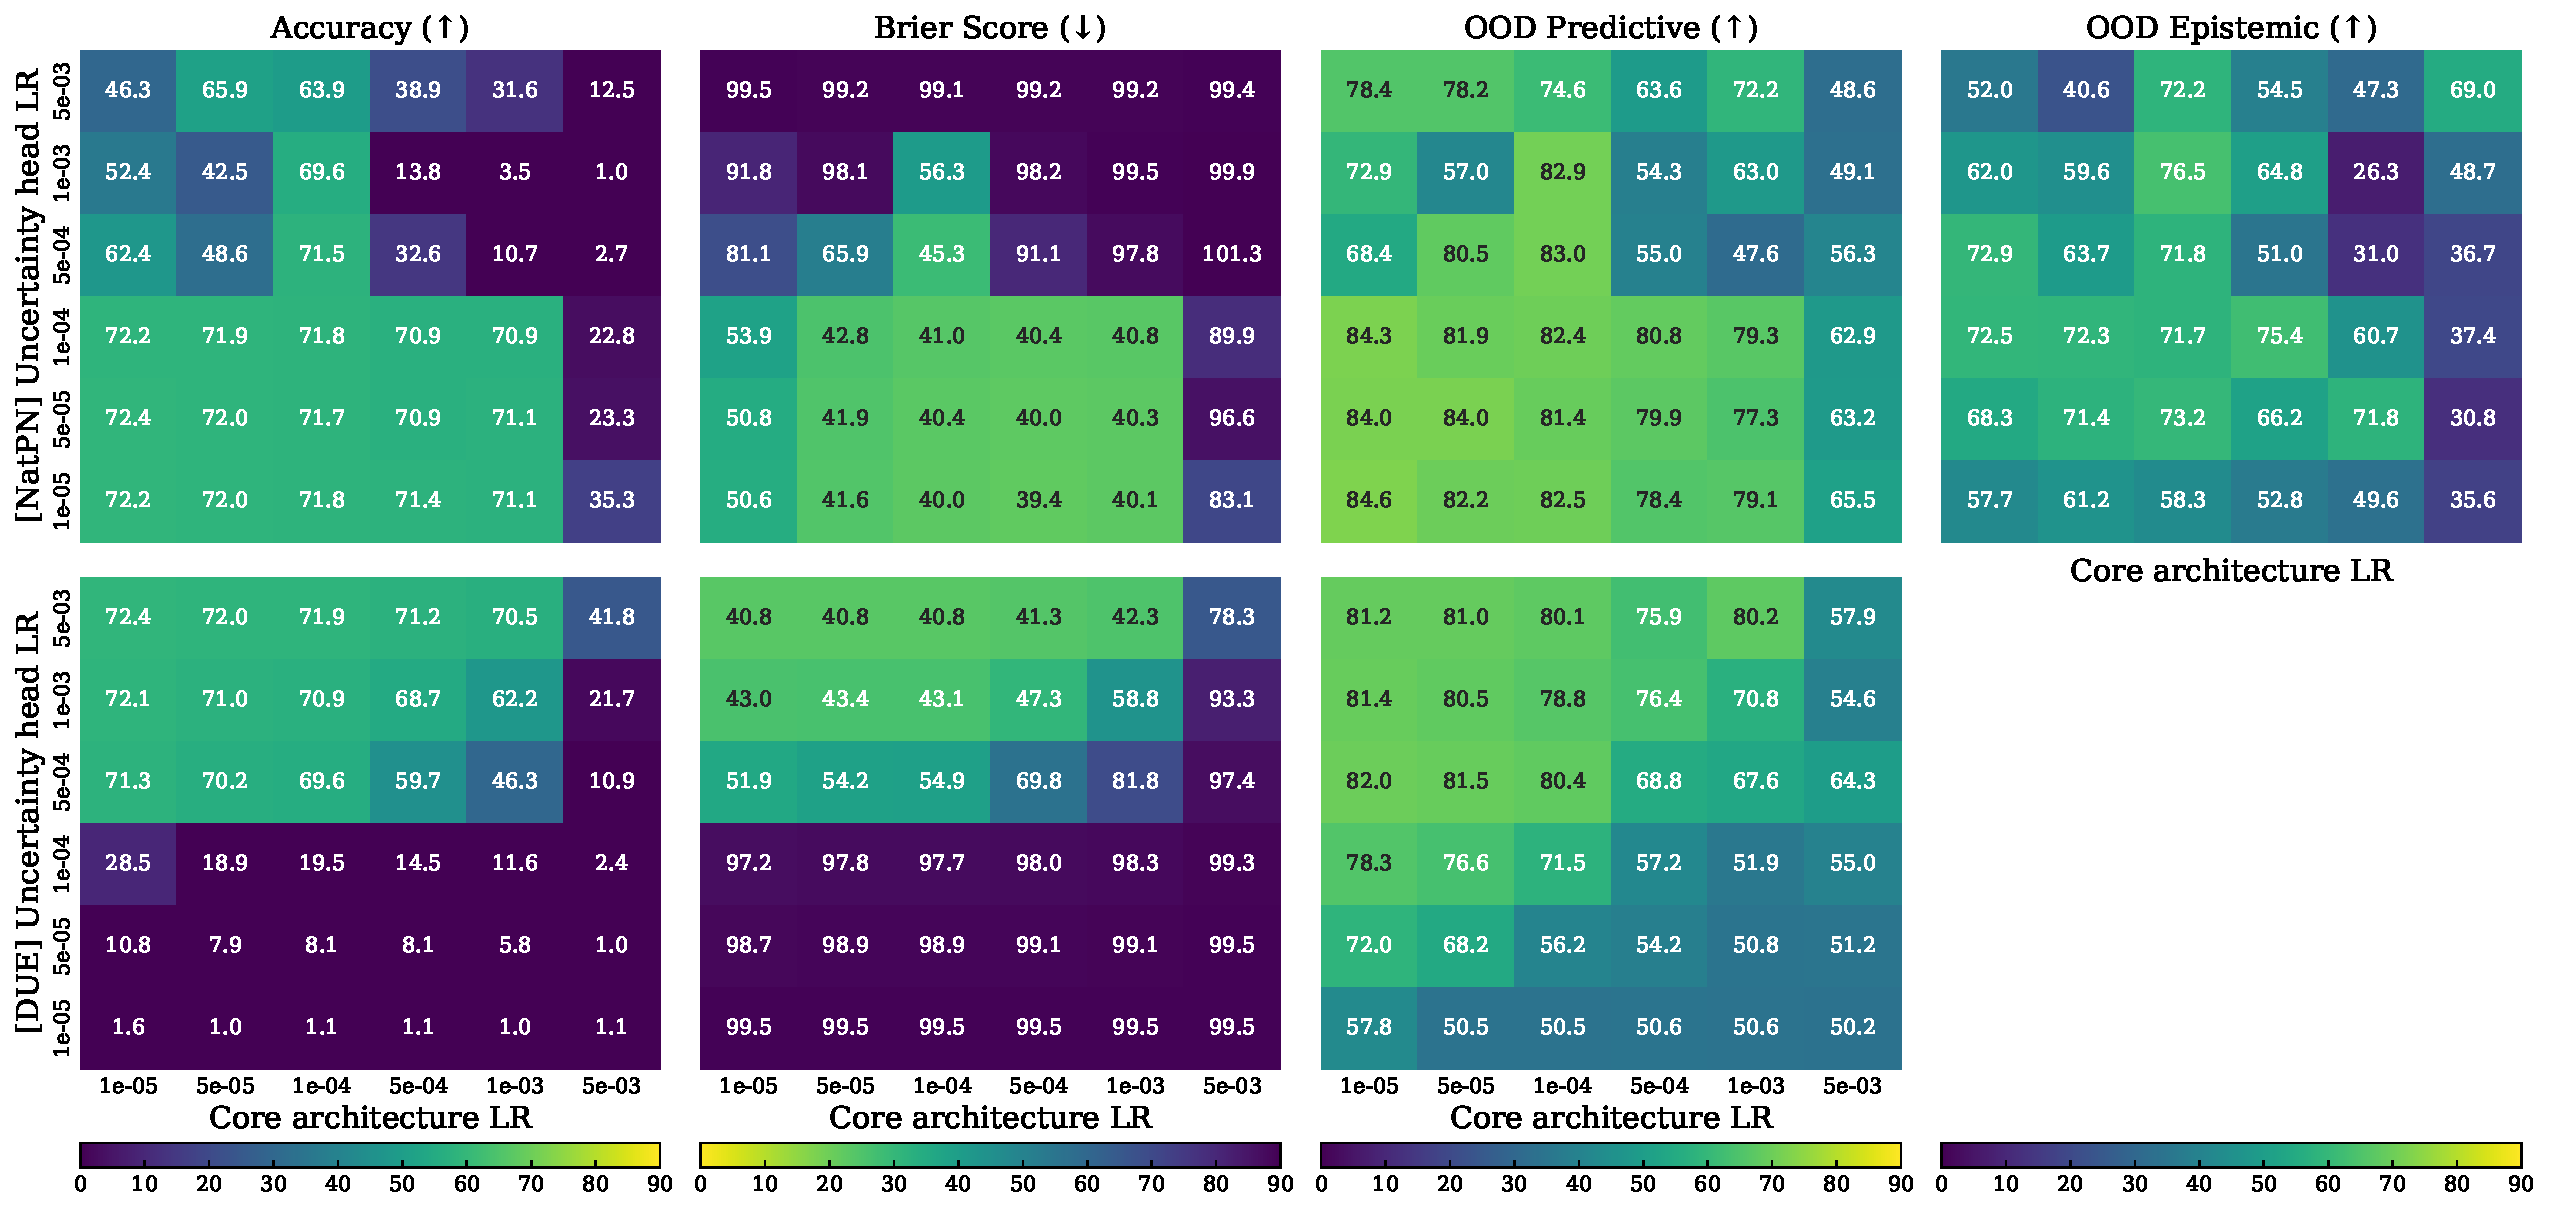
\includegraphics[width=0.8\linewidth]{sections/008_iclr2023/figures/decoupled_test.pdf}
    \caption{Results of DUMS on CIFAR100 with ResNet18 when \textbf{decoupling learning rates} of the core architecture and the uncertainty head. Decoupling learning rates improve DUMs performance. }
    \label{fig:decoupled_test}
\end{figure}

\textbf{Training schemes.} We compare two settings: the \textit{joint} training in which we jointly train the weights of the core architecture and uncertainty head, and the \textit{sequential} training in which we only train the uncertainty head by keeping the weights of the pretrained core architecture fixed. For each of the setting, we apply two additional techniques to stabilize the training: adding a \textit{batch normalization} to the last layer of the encoder to enforce latent representations to locate in a normalized region \citep{ioffe2015bn,NatPN2021}, and \textit{resetting the last layer} to retrain its weights to improve robustness to spurious correlation \citep{kirichenko2022reset}. We show the results for CIFAR100 as ID and five difference OOD datasets with the ResNet18 as core architecture in \cref{tab:training_schema} and additional results in the appendix \cref{tab:training_schema_ood}.
\underline{\textit{Observation:}} We observe that, compared to its sequential counterpart, joint training consistently improves DUMs performance for most metrics, thus suggesting that joint training should be preferred in practice for DUMs. Furthermore, while the GP-based method DUE does not benefit from stabilization techniques, we observe that they can significantly increase performance of the density-based method NatPN. This behavior is intuitively explained by the practical difficulty to accurately fit densities in high dimensional latent space. This can be significantly improved by using more powerful density estimator (see \cref{tab:normalizing_flow} in appendix).

\textbf{Pretraining schemes.} We compare multiple training schemes which differ in terms of \emph{amount} and \emph{quality} of data used for pretraining. Hence, we do not pretrain the core architecture or pretrain it with 10\% of CIFAR100, 100\% of CIFAR100 without and with Gaussian noise, or ImageNet. We show the results for CIFAR100 as ID and five different OOD datasets with ResNet50 as core architecture in \cref{tab:training_pretrain} and additional results in the appendix \cref{tab:training_pretrain_ood}.
\underline{\textit{Observation:}} We observe that, while too few data for pretraining does not improve final performance of DUMs, the overall performance significantly increase when the encoder is pretrained with high quantity and high quality of data.  Similarly to \citet{why-nf-fail-ood}, this suggests that the embedding quality is important to improve uncertainty quantification. Here, we show additionally that embeddings pretrained with many high quality data are crucial to facilitate the prediction of the uncertainty head.

\begin{table}[!htp]\centering
    \caption{Results of DUMs on CIFAR100 with ResNet18 under different \textbf{training schemes} using \textit{joint/sequential} training with no additional layer, an additional batch norm layer, or resetting the last layer. Gray cells indicate the best between \textit{joint/sequential} while bold numbers indicate the best overall. OOD results are averaged over OOD datasets. We observe that joint training works best and stabilization techniques can improve performances.}
    \label{tab:training_schema}
    \tiny
    
    \resizebox{0.9\textwidth}{!}{%
    \begin{tabular}{llccccc}
        \toprule
        \textbf{Method} &\textbf{Train Schema} &\textbf{Accuracy ($\uparrow$)} &\textbf{Brier Score ($\downarrow$)} &\textbf{OOD Pred. ($\uparrow$)} &\textbf{OOD Epis. ($\uparrow$)} \\
        \midrule
        \multirow{6}{*}{NatPN} 
        & joint &71.12 $\pm$ 0.18 & \cellcolor{mycolor}41.06 $\pm$ 0.18 & \cellcolor{mycolor}75.17 $\pm$ 1.60 & \cellcolor{mycolor}63.94 $\pm$ 2.80 \\
        & joint + bn &71.60 $\pm$ 0.14 &\cellcolor{mycolor}41.11 $\pm$ 0.12 & 74.22 $\pm$ 0.94 & \cellcolor{mycolor}66.17 $\pm$ 2.55 \\
        & joint + reset &71.61 $\pm$ 0.18 & \cellcolor{mycolor}\textbf{40.76 $\pm$ 0.18} &\cellcolor{mycolor}\textbf{75.35 $\pm$ 0.71} & \cellcolor{mycolor}\textbf{69.02 $\pm$ 1.49} \\
        % \cmidrule[0.1pt](lr){2-6}
        & sequential & \cellcolor{mycolor}\textbf{72.00 $\pm$ 0.19} &42.20 $\pm$ 0.09 &75.09 $\pm$ 0.86 &53.49 $\pm$ 2.56 \\
        & sequential + bn & \cellcolor{mycolor}71.98 $\pm$ 0.18 & 42.39 $\pm$ 0.11 & \cellcolor{mycolor}75.01 $\pm$ 0.86 &52.34 $\pm$ 2.81 \\
        & sequential + reset & \cellcolor{mycolor}71.79 $\pm$ 0.17 &40.95 $\pm$ 0.14 &74.63 $\pm$ 0.85 &61.90 $\pm$ 2.14 \\
        \midrule
        \multirow{6}{*}{DUE} 
        & joint & \cellcolor{mycolor}\textbf{72.33 $\pm$ 0.11} & \cellcolor{mycolor}\textbf{40.80 $\pm$ 0.11} &74.74 $\pm$ 0.89 &- \\
        & joint + bn & \cellcolor{mycolor}72.30 $\pm$ 0.09 & \cellcolor{mycolor}40.85 $\pm$ 0.12 &74.63 $\pm$ 0.95 &- \\
        & joint + reset & \cellcolor{mycolor}71.94 $\pm$ 0.12 & \cellcolor{mycolor}41.43 $\pm$ 0.12 &74.89 $\pm$ 0.76 &- \\
        % \cmidrule[0.1pt](lr){2-6}
        & sequential &72.07 $\pm$ 0.10 &41.66 $\pm$ 0.10 & \cellcolor{mycolor}74.82 $\pm$ 0.90 &- \\
        & sequential + bn &72.04 $\pm$ 0.13 &41.73 $\pm$ 0.11 & \cellcolor{mycolor}74.88 $\pm$ 0.95 &- \\
        & sequential + reset &71.56 $\pm$ 0.14 &42.30 $\pm$ 0.11 & \cellcolor{mycolor}\textbf{75.08 $\pm$ 1.01} &- \\
        \bottomrule
    \end{tabular}
    }
\end{table}

\begin{table}[!htp]\centering
    \caption{Results of DUMs with ResNet50 under different \textbf{pretraining schemes} using no pretraining, pretraining on 10\% of CIFAR100, 100\% of CIFAR100 without Gaussian noise and with Gaussian noise, or ImageNet. OOD results are averaged over OOD datasets. Bold numbers indicate best results among all settings. We observe that high quantity and high quality of data can improve performances.}
    \label{tab:training_pretrain}
    \tiny
    
    \resizebox{0.9\textwidth}{!}{%
    \begin{tabular}{llccccc}\toprule
        \textbf{Method} &\textbf{Pretrain Schema} &\textbf{Accuracy ($\uparrow$)} &\textbf{Brier Score ($\downarrow$)} &\textbf{OOD Pred. ($\uparrow$)} &\textbf{OOD Epis. ($\uparrow$)} \\
        \midrule
        \multirow{6}{*}{NatPN} &None &78.45 $\pm$ 1.94 &30.16 $\pm$ 2.57 &79.85 $\pm$ 3.30 &85.81 $\pm$ 2.05 \\
        &C100 (10\%) &67.25 $\pm$ 0.71 &44.69 $\pm$ 0.94 &68.10 $\pm$ 1.90 &78.50 $\pm$ 3.27 \\
        &C100 (100\%) + $\gN(0.5)$ &72.50 $\pm$ 1.07 &39.36 $\pm$ 1.43 &68.66 $\pm$ 3.76 &73.54 $\pm$ 1.84 \\
        &C100 (100\%) + $\gN(0.1)$ &75.25 $\pm$ 0.61 &35.99 $\pm$ 0.88 &69.78 $\pm$ 4.65 &75.81 $\pm$ 2.85 \\
        &C100 (100\%) &76.31 $\pm$ 0.45 &34.32 $\pm$ 0.51 &78.95 $\pm$ 3.19 &76.91 $\pm$ 2.64 \\
        &ImageNet &\textbf{84.22 $\pm$ 0.12} &\textbf{23.67 $\pm$ 0.27} &\textbf{84.95 $\pm$ 1.48} &\textbf{89.08 $\pm$ 0.70} \\
        \midrule
        \multirow{6}{*}{DUE} &None &72.41 $\pm$ 0.24 &47.35 $\pm$ 0.25 &80.04 $\pm$ 1.28 &- \\
        &C100 (10\%) &63.86 $\pm$ 0.58 &50.94 $\pm$ 0.53 &72.44 $\pm$ 1.32 &- \\
        &C100 (100\%) &76.38 $\pm$ 0.35 &36.89 $\pm$ 0.50 &81.71 $\pm$ 1.87 &- \\
        &C100 (100\%) + $\gN(0.5)$ &72.10 $\pm$ 1.00 &42.48 $\pm$ 1.18 &74.89 $\pm$ 1.97 &- \\
        &C100 (100\%) + $\gN(0.1)$ &75.31 $\pm$ 0.91 &38.31 $\pm$ 1.22 &79.43 $\pm$ 1.93 &- \\
        &ImageNet &\textbf{82.42 $\pm$ 0.14} &\textbf{28.09 $\pm$ 0.19} &\textbf{90.24 $\pm$ 0.51} &- \\
        \bottomrule
        \end{tabular}
    }
\end{table}






% \begin{table}[!htb]
% \centering
% \tiny

% \begin{minipage}[t]{0.48\textwidth}
% \caption{Results of DUMs on CIFAR100 with ResNet18 under different \textbf{training schemes} using \textit{joint/sequential} training with no additional layer, an additional batch norm layer, or resetting the last layer. Gray cells indicate the best between \textit{joint/sequential} while bold numbers indicate the best overall. OOD results are averaged over OOD datasets. We observe that joint training works best and stabilization techniques can improve performances.}
% \label{tab:training_schema}
% \resizebox{\textwidth}{!}{%
% \begin{tabular}{llccccc}
% \toprule
% \textbf{Method} &\textbf{Train Schema} &\textbf{Accuracy ($\uparrow$)} &\textbf{Brier Score ($\downarrow$)} &\textbf{OOD Pred. ($\uparrow$)} &\textbf{OOD Epis. ($\uparrow$)} \\
% \midrule
% \multirow{6}{*}{NatPN} 
% & joint &71.12 $\pm$ 0.18 & \cellcolor{mycolor}41.06 $\pm$ 0.18 & \cellcolor{mycolor}75.17 $\pm$ 1.60 & \cellcolor{mycolor}63.94 $\pm$ 2.80 \\
% & joint + bn &71.60 $\pm$ 0.14 &\cellcolor{mycolor}41.11 $\pm$ 0.12 & 74.22 $\pm$ 0.94 & \cellcolor{mycolor}66.17 $\pm$ 2.55 \\
% & joint + reset &71.61 $\pm$ 0.18 & \cellcolor{mycolor}\textbf{40.76 $\pm$ 0.18} &\cellcolor{mycolor}\textbf{75.35 $\pm$ 0.71} & \cellcolor{mycolor}\textbf{69.02 $\pm$ 1.49} \\
% % \cmidrule[0.1pt](lr){2-6}
% & sequential & \cellcolor{mycolor}\textbf{72.00 $\pm$ 0.19} &42.20 $\pm$ 0.09 &75.09 $\pm$ 0.86 &53.49 $\pm$ 2.56 \\
% & sequential + bn & \cellcolor{mycolor}71.98 $\pm$ 0.18 & 42.39 $\pm$ 0.11 & \cellcolor{mycolor}75.01 $\pm$ 0.86 &52.34 $\pm$ 2.81 \\
% & sequential + reset & \cellcolor{mycolor}71.79 $\pm$ 0.17 &40.95 $\pm$ 0.14 &74.63 $\pm$ 0.85 &61.90 $\pm$ 2.14 \\
% \midrule
% \multirow{6}{*}{DUE} 
% & joint & \cellcolor{mycolor}\textbf{72.33 $\pm$ 0.11} & \cellcolor{mycolor}\textbf{40.80 $\pm$ 0.11} &74.74 $\pm$ 0.89 &- \\
% & joint + bn & \cellcolor{mycolor}72.30 $\pm$ 0.09 & \cellcolor{mycolor}40.85 $\pm$ 0.12 &74.63 $\pm$ 0.95 &- \\
% & joint + reset & \cellcolor{mycolor}71.94 $\pm$ 0.12 & \cellcolor{mycolor}41.43 $\pm$ 0.12 &74.89 $\pm$ 0.76 &- \\
% % \cmidrule[0.1pt](lr){2-6}
% & sequential &72.07 $\pm$ 0.10 &41.66 $\pm$ 0.10 & \cellcolor{mycolor}74.82 $\pm$ 0.90 &- \\
% & sequential + bn &72.04 $\pm$ 0.13 &41.73 $\pm$ 0.11 & \cellcolor{mycolor}74.88 $\pm$ 0.95 &- \\
% & sequential + reset &71.56 $\pm$ 0.14 &42.30 $\pm$ 0.11 & \cellcolor{mycolor}\textbf{75.08 $\pm$ 1.01} &- \\
% \bottomrule
% \end{tabular}
% }\end{minipage}\quad%
% %
% %
% \begin{minipage}[t]{0.48\textwidth}
% \caption{Results of DUMs with ResNet50 under different \textbf{pretraining schemes} using no pretraining, pretraining on 10\% of CIFAR100, 100\% of CIFAR100 without Gaussian noise and with Gaussian noise, or ImageNet. OOD results are averaged over OOD datasets. Bold numbers indicate best results among all settings. We observe that high quantity and high quality of data can improve performances.}
% \label{tab:training_pretrain}

% \resizebox{\textwidth}{!}{%
% \begin{tabular}{llccccc}\toprule
% \textbf{Method} &\textbf{Pretrain Schema} &\textbf{Accuracy ($\uparrow$)} &\textbf{Brier Score ($\downarrow$)} &\textbf{OOD Pred. ($\uparrow$)} &\textbf{OOD Epis. ($\uparrow$)} \\
% \midrule
% \multirow{6}{*}{NatPN} &None &78.45 $\pm$ 1.94 &30.16 $\pm$ 2.57 &79.85 $\pm$ 3.30 &85.81 $\pm$ 2.05 \\
% &C100 (10\%) &67.25 $\pm$ 0.71 &44.69 $\pm$ 0.94 &68.10 $\pm$ 1.90 &78.50 $\pm$ 3.27 \\
% &C100 (100\%) + $\gN(0.5)$ &72.50 $\pm$ 1.07 &39.36 $\pm$ 1.43 &68.66 $\pm$ 3.76 &73.54 $\pm$ 1.84 \\
% &C100 (100\%) + $\gN(0.1)$ &75.25 $\pm$ 0.61 &35.99 $\pm$ 0.88 &69.78 $\pm$ 4.65 &75.81 $\pm$ 2.85 \\
% &C100 (100\%) &76.31 $\pm$ 0.45 &34.32 $\pm$ 0.51 &78.95 $\pm$ 3.19 &76.91 $\pm$ 2.64 \\
% &ImageNet &\textbf{84.22 $\pm$ 0.12} &\textbf{23.67 $\pm$ 0.27} &\textbf{84.95 $\pm$ 1.48} &\textbf{89.08 $\pm$ 0.70} \\
% \midrule
% \multirow{6}{*}{DUE} &None &72.41 $\pm$ 0.24 &47.35 $\pm$ 0.25 &80.04 $\pm$ 1.28 &- \\
% &C100 (10\%) &63.86 $\pm$ 0.58 &50.94 $\pm$ 0.53 &72.44 $\pm$ 1.32 &- \\
% &C100 (100\%) &76.38 $\pm$ 0.35 &36.89 $\pm$ 0.50 &81.71 $\pm$ 1.87 &- \\
% &C100 (100\%) + $\gN(0.5)$ &72.10 $\pm$ 1.00 &42.48 $\pm$ 1.18 &74.89 $\pm$ 1.97 &- \\
% &C100 (100\%) + $\gN(0.1)$ &75.31 $\pm$ 0.91 &38.31 $\pm$ 1.22 &79.43 $\pm$ 1.93 &- \\
% &ImageNet &\textbf{82.42 $\pm$ 0.14} &\textbf{28.09 $\pm$ 0.19} &\textbf{90.24 $\pm$ 0.51} &- \\
% \bottomrule
% \end{tabular}
% }\end{minipage}
% \end{table}

% \begin{table}[!htp]\centering
% \caption{\textbf{Pretrain schema.} Both DUMs benefits from the quantity of data under the ImageNet pretrained encoder. The reported OOD results are an average over all the independent OOD dataset result. The encoder ResNet50 from torchvision is used for the schemas.}
% \label{tab:training_pretrain}
% \tiny
% \begin{tabular}{llccccc}\toprule
% \textbf{Model} &\textbf{Pretrain Schema} &\textbf{Accuracy} &\textbf{Brier Score} &\textbf{OOD Pred.} &\textbf{OOD Epis.} \\
% \midrule
% \multirow{4}{*}{NatPN} &None &78.45 $\pm$ 1.94 &30.16 $\pm$ 2.57 &79.85 $\pm$ 3.30 &85.81 $\pm$ 2.05 \\
% &C100 (10\%) &67.25 $\pm$ 0.71 &44.69 $\pm$ 0.94 &68.10 $\pm$ 1.90 &78.50 $\pm$ 3.27 \\
% &C100 (100\%) &76.31 $\pm$ 0.45 &34.32 $\pm$ 0.51 &78.95 $\pm$ 3.19 &76.91 $\pm$ 2.64 \\
% &\textbf{ImageNet} &\textbf{84.22 $\pm$ 0.12} &\textbf{23.67 $\pm$ 0.27} &\textbf{84.95 $\pm$ 1.48} &\textbf{89.08 $\pm$ 0.70} \\
% \midrule
% \multirow{4}{*}{DUE} &None &72.41 $\pm$ 0.24 &47.35 $\pm$ 0.25 &80.04 $\pm$ 1.28 &- \\
% &C100 (10\%) &63.86 $\pm$ 0.58 &50.94 $\pm$ 0.53 &72.44 $\pm$ 1.32 &- \\
% &C100 (100\%) &76.38 $\pm$ 0.35 &36.89 $\pm$ 0.50 &81.71 $\pm$ 1.87 &- \\
% &\textbf{ImageNet} &\textbf{82.42 $\pm$ 0.14} &\textbf{28.09 $\pm$ 0.19} &\textbf{90.24 $\pm$ 0.51} &- \\
% \bottomrule
% \end{tabular}
% \end{table}

% ENCODER --------------------------------
\section{Architecture for DUMs}
\label{sec:architecture}

In this section, we study the impact of the architecture component in DUMs. To this end, we look at different \emph{latent dimensions}, different \emph{architectural types and size}, and applying different \emph{regularization constraints} to avoid \textit{feature collapse} \citep{due}. 

\textbf{Latent dimension.} We vary the dimension of the output space of the core architecture. We show the results for each pair of ID dataset and its distribution shifted OOD dataset (MNIST/CMNIST, CIFAR/CIFAR-C, CamelyonID/CamelyonOOD) with the core architecture ResNet18 for MNIST/CIFAR, and WideResNet-28-10 for Camelyon in \cref{fig:latent} and additional uncertainty estimation results in the appendix \cref{fig:latent_ood}. \underline{\textit{Observation:}} We observe that increasing the latent dimensions leads to improvement for DUMs on ID and OOD datasets with particularly significant improvement for NatPN (see \cref{fig:latent}). This suggests that higher latent dimensions are more expressive by encoding more information. However, we observe that  a too high latent dimension can degrade OOD detection performance by causing numerical instabilities in the training (see \cref{fig:latent_ood}), suggesting a trade-off between OOD generalization and OOD detection.

\begin{figure}[!htb]
    \centering
    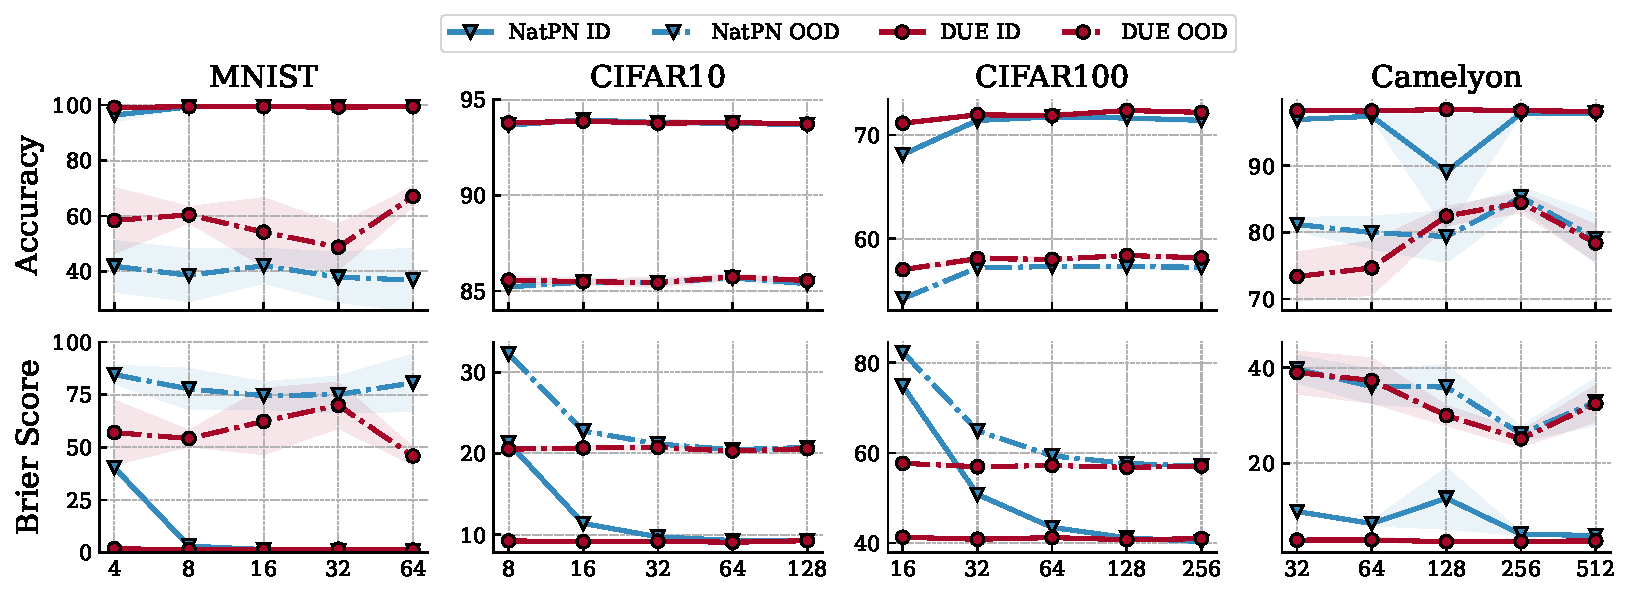
\includegraphics[width=0.9\textwidth]{sections/008_iclr2023/figures/latent.pdf}
    \caption{Results of DUMs when varying the \textbf{latent dimension size}. We observe that increasing the latent dimension consistently leads to similar or better predictive performance.}
    \label{fig:latent}
\end{figure}
    % We observe that increasing the latent dimension can increase the predictive performance.}

\textbf{Architecture type and size.} We compare the influence of the type and size of the core architecture on the performance of DUMs. We consider residual, convolutional, and transformer architectures like ResNet18, ResNet50, EfficientNetV2, and Swin \citep{resnet, tan2021effcientnet, liu2021swin}. We show the results for DUMs trained on CIFAR100 as ID with the different core architectures in \cref{tab:encoder_architecture} and additional results at appendix \cref{tab:encoder_architecture_ood}. \underline{\textit{Observation:}} We observe that models with more parameters achieve better results. In particular, ResNet50 achieves significantly better results than ResNet18. Further, more recent core architectures like EfficientNetV2 and Swin are better calibrated and more expressive leading to a better overall performance. This can be explained by the fact that they are more expressive and provide more informative embeddings for the uncertainty head to operate on. This aligns with \citet{minderer2021revisiting} which states that the architecture type is important for the calibration properties. 

% \begin{wraptable}{r}{0.5\textwidth}
% \centering
% \caption{\textbf{Encoder Architecture Comparison.} Recent architectures are better calibrated with similar or better uncertainty estimation. The reported OOD results are an average over all the independent OOD dataset result.}
% \label{tab:encoder_architecture}
% \tiny
% \begin{tabular}{lcccccc}\toprule
% \textbf{Encoder} &\textbf{Param.} &\textbf{Brier Score} &\textbf{OOD Pred.} &\textbf{OOD Epis.} \\
% \midrule
% ResNet18 &11.6M &33.69 $\pm$ 0.15 &87.49 $\pm$ 1.90 &81.79 $\pm$ 1.38 \\
% ResNet50 &25.5M &23.67 $\pm$ 0.27 &84.95 $\pm$ 1.48 &89.08 $\pm$ 0.70 \\
% \textbf{EffNet\_V2\_S} &\textbf{21.4M} &\textbf{17.08 $\pm$ 0.10} &\textbf{87.79 $\pm$ 0.77} &89.47 $\pm$ 0.59 \\
% Swin\_T &28.2M &18.48 $\pm$ 0.06 &85.91 $\pm$ 1.17 &\textbf{90.23 $\pm$ 0.81} \\
% \midrule
% ResNet18 &11.6M &36.57 $\pm$ 0.15 &88.04 $\pm$ 0.67 &- \\
% ResNet50 &25.5M &28.09 $\pm$ 0.19 &\textbf{90.24 $\pm$ 0.51} &- \\
% \textbf{EffNet\_V2\_S} &21.4M &\textbf{21.07 $\pm$ 0.06} &89.43 $\pm$ 0.67 &- \\
% Swin\_T &28.2M &23.23 $\pm$ 0.05 &89.90 $\pm$ 0.36 &- \\
% \bottomrule
% \end{tabular}
% \end{wraptable}

\begin{table}[!htp]\centering
\caption{Results of DUMs for different \textbf{architecture types.} including residual, convolutional, and transformer architectures on CIFAR100.  OOD results are averaged over OOD datasets. Bold numbers indicate best results among all settings. Larger and more recent architectures are better calibrated with similar or better uncertainty estimation.}
\label{tab:encoder_architecture}
\tiny

\resizebox{0.9\textwidth}{!}{%
\begin{tabular}{llcccccc}\toprule
\textbf{Method} &\textbf{Architecture} &\textbf{\#Parameters} &\textbf{Accuracy ($\uparrow$)} &\textbf{Brier Score ($\downarrow$)} &\textbf{OOD Pred. ($\uparrow$)} &\textbf{OOD Epis. ($\uparrow$)} \\
\midrule
\multirow{4}{*}{NatPN} &ResNet18 &11.6M &80.31 $\pm$ 0.09 &33.69 $\pm$ 0.15 &87.49 $\pm$ 1.90 &81.79 $\pm$ 1.38 \\
&ResNet50 &25.5M &84.22 $\pm$ 0.12 &23.67 $\pm$ 0.27 &84.95 $\pm$ 1.48 &89.08 $\pm$ 0.70 \\
&EffNet\_V2\_S &21.4M &\textbf{88.43 $\pm$ 0.10} &\textbf{17.08 $\pm$ 0.10} &\textbf{87.79 $\pm$ 0.77} &89.47 $\pm$ 0.59 \\
&Swin\_T &28.2M &87.99 $\pm$ 0.09 &18.48 $\pm$ 0.06 &85.91 $\pm$ 1.17 &\textbf{90.23 $\pm$ 0.81} \\
\midrule
\multirow{4}{*}{DUE} &ResNet18 &11.6M &78.85 $\pm$ 0.19 &36.57 $\pm$ 0.15 &88.04 $\pm$ 0.67 &- \\
&ResNet50 &25.5M &82.42 $\pm$ 0.14 &28.09 $\pm$ 0.19 &\textbf{90.24 $\pm$ 0.51} &- \\
&EffNet\_V2\_S &21.4M &86.92 $\pm$ 0.08 &\textbf{21.07 $\pm$ 0.06} &89.43 $\pm$ 0.67 &- \\
&Swin\_T &28.2M &\textbf{86.93 $\pm$ 0.05} &23.23 $\pm$ 0.05 &89.90 $\pm$ 0.36 &- \\
\bottomrule
\end{tabular}
}
\end{table}

\textbf{Regularization constraints.} \emph{Feature collapse} is a phenomenon where a model may discard important parts of the input information during its training phase, which may degrade OOD detection performance \citep{due}. Two techniques to avoid feature collapses are \textit{bi-Lipschitz} constraints via combining residual connections and lipschitz constraints \citep{uncertainty-distance-awareness}, and \textit{reconstruction} constraints via adding an additional reconstruction term in the loss \citep{postels2020mir}. We show the results for DUMs trained on the datasets MNIST and CIFAR100 with ResNet18 in \cref{fig:bi,fig:rec} and additional results for other datasets (Toy dataset, CIFAR10, Camelyon) at \cref{subsec:appendix_encoder}. \underline{\textit{Observation:}} We observe that the reconstruction technique is not capable to avoid feature collapse. Indeed, we show  that, even with reconstruction constraints, some (non-discriminative) features can completely collapse (see \cref{fig:rec_toy_collapse,fig:rec_toy} for toy examples). Hence, while this method can lead to small OOD improvements on simple tasks (see e.g. MNIST in \cref{fig:rec}), this benefit does not generalize to more complex tasks (see e.g. CIFAR100 in \cref{fig:rec}). In contrast, we observe that bilipschitz constraints indeed mitigate the collapse of features (see \cref{fig:bi_toy_collapse,fig:bi_toy} for toy examples), leading to similar or higher OOD detection performance (see \cref{fig:bi}). The mitigation of feature collapse can be mostly assigned to the residual connection constraints. However, bilipschitz constraints can improve OOD detection results on simple tasks (e.g. MNIST, CIFAR10), it degrades OOD generalization performance (see \cref{fig:bi}) and does not significantly improve OOD detection on more complex tasks (see e.g. Camelyon, CIFAR100 in \cref{fig:bi_bar_full}). Intuitively, maintaining features which are not discriminative to the task might introduce spurious correlations, thus degrading performances. E.g. enforces the architecture to encode the color feature in the latent space decreases the performance of the OOD CMNIST datasets after training on the ID MNIST dataset. 

\begin{figure}
\begin{minipage}[t]{0.48\textwidth}
    \centering
    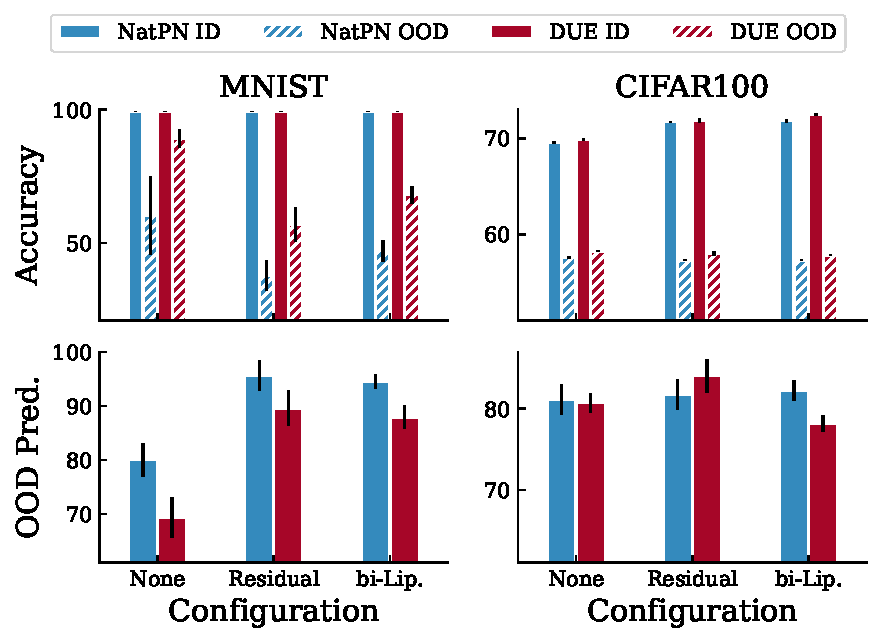
\includegraphics[width=0.9\textwidth]{sections/008_iclr2023/figures/bi_bar_short.pdf}
    \caption{Results OOD generalization and detection of DUMs with none, residual and bi-lipschitz \textbf{architecture constraints} on MNIST/CMNIST and CIFAR/CIFAR-C. Bi-lipschitz can improve OOD detection by mitigating feature collapse (see \cref{fig:bi_toy}) at the expense of degrading OOD generalization.}
    \label{fig:bi}
\end{minipage}\quad%
%
\begin{minipage}[t]{0.48\textwidth}
    \centering
    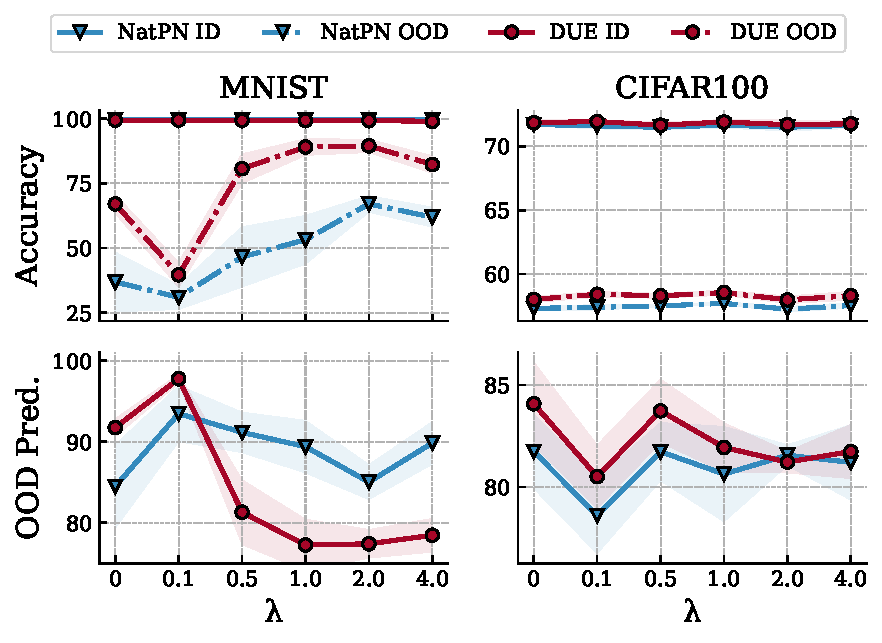
\includegraphics[width=0.9\textwidth]{sections/008_iclr2023/figures/reconst_short.pdf}
    \caption{Results OOD generalization and detection of DUMs with reconstruction \textbf{architecture constraints} on MNIST/CMNIST and CIFAR/CIFAR-C. Increasing the reconstruction strength $\lambda$ improves the OOD generalization on simple MNIST/CMNIST dataset but fails for complex datasets. Reconstruction fails to improve OOD detection since it does not avoid feature collapse (see \cref{fig:rec_toy}). }
    \label{fig:rec}
\end{minipage}
\end{figure}

% PRIOR -----------------------------------
\section{Prior for DUMs}
\label{sec:prior}

In this section, we study the effect that the prior component has in DUMs. More specifically, we investigate the relationships between aleatoric uncertainty and the prior specified for DUMs. In particular, this is motivated by \citet{kapoor2022prior_cpe} which shows that using priors that forces model to be confident on the training data points can improve its performance by explicitly accounting for aleatoric uncertainty.
To this end, we look at \textit{entropy regularization} defining a training prior in the loss, \textit{prior evidence} and \textit{kernel function} defining a functional prior in the uncertainty head.

\textbf{Prior.} We compare different prior specifications including \textit{entropy regularization} defining a training prior in the loss, \textit{prior evidence} and \textit{kernel function} defining a functional prior in the uncertainty head. Entropy regularization is the entropy term $H(Q)$ in the Bayesian loss used to train NatPN which encourages a (uniform) prior distributions with high entropy \citep{charpentier2022natpn}. We control the strength of the regularization factor $\lambda$. Further, NatPN also explicitly defines a prior via the parameters $\chi^{prior}$ and $n^{prior}$. While  $\chi^{prior}$ defines the default categorical prediction via a uniform categorical distribution, the evidence parameter $n^{prior}$ defines the prior number of pseudo-observations and can be varied. Finally, we vary the prior of DUE by using different kernel functions in the learned GP including Matern kernel, RQ kernel, and RBF \citep{rasmussen2006gp}. \underline{\textit{Observation:}} Contrary to other Bayesian neural networks \citep{kapoor2022prior_cpe}, we observe that predictive and uncertainty performances of DUMs are not very sensitive to the prior specification (see \cref{fig:prior_ood,fig:prior_ood_brier,tab:kernel}), thus suggesting a higher robustness to prior mispecification. Nonetheless, a too strong entropy regularization toward an uniform prior degrades more performance of DUMs trained on dataset with low label noise than on high label noise. This suggests that a too high discrepancy between the model prior and the dataset aleatoric uncertainties can impact performance.

\begin{figure}[!htb]
    \centering
    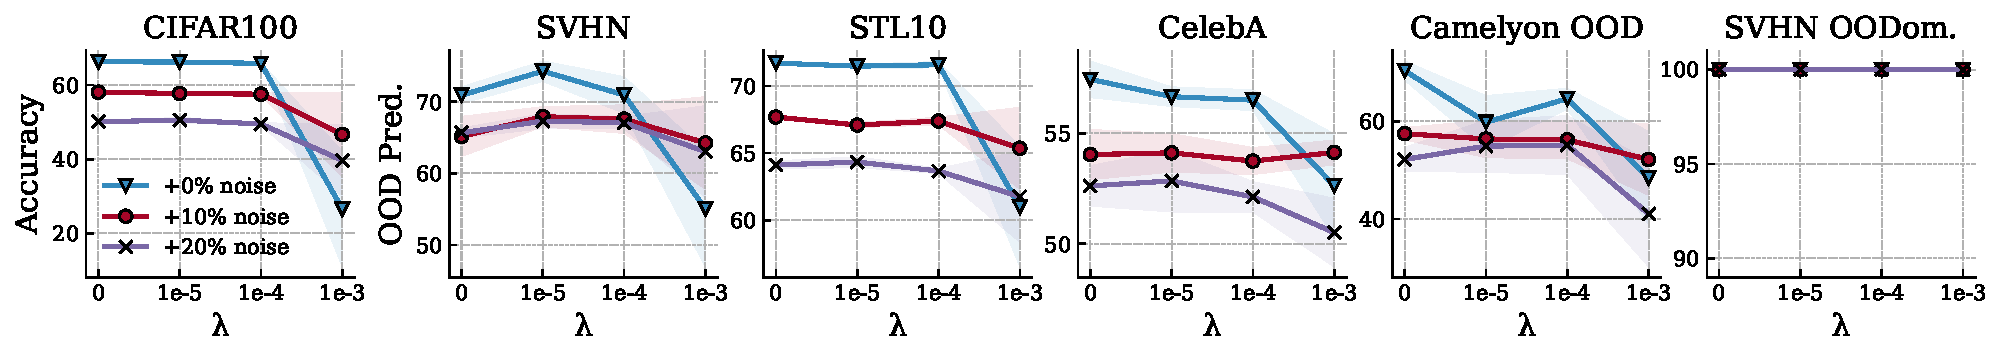
\includegraphics[width=\textwidth]{sections/008_iclr2023/figures/prior_entropy_acc_pred.pdf}
    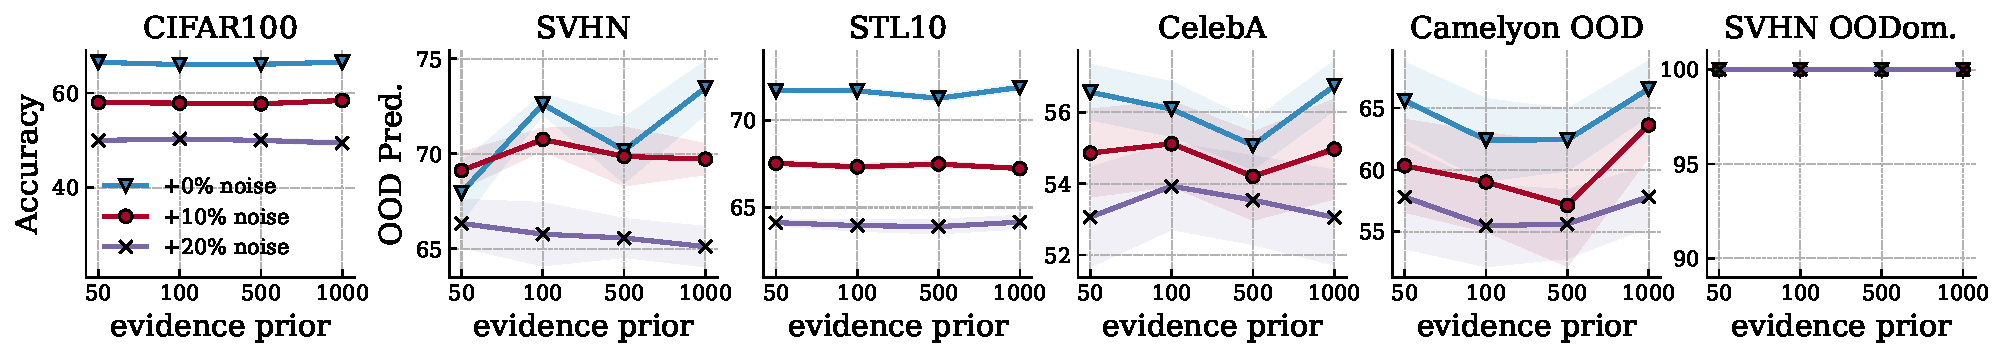
\includegraphics[width=\textwidth]{sections/008_iclr2023/figures/prior_pseudo_acc_pred.pdf}
    
    \caption{Results of enforcing different \textbf{prior} in NatPN on CIFAR100 by changing the (top) \textit{entropy regularization} $\lambda$ and the (bottom) \textit{evidence prior} $n^{prior}$. Different priors do not lead consistent results improvements.}
    \label{fig:prior_ood}
\end{figure}
 \vspace{-3mm}
\begin{table}[!htp]\centering
\caption{Results of enforcing different \textbf{prior} in DUE on CIFAR100 and Camelyon by changing the kernel function. OOD results are averaged over OOD datasets. Different priors lead to similar performance. }
\label{tab:kernel}
\vspace{-0mm}
\tiny
\resizebox{0.9\textwidth}{!}{%
\begin{tabular}{lcccccc}\toprule
&\multicolumn{3}{c}{\textbf{CIFAR100}} &\multicolumn{3}{c}{\textbf{Camelyon}} \\
\cmidrule(lr){2-4}\cmidrule(lr){5-7}
\textbf{Kernel} &\textbf{Accuracy ($\uparrow$)} &\textbf{Brier Score ($\downarrow$)} &\textbf{OOD Pred. ($\uparrow$)} &\textbf{Accuracy ($\uparrow$)} &\textbf{Brier Score ($\downarrow$)} &\textbf{OOD Pred. ($\uparrow$)} \\
\midrule
Matern52 &71.80 $\pm$ 0.18 &41.37 $\pm$ 0.24 &75.90 $\pm$ 1.18 &79.81 $\pm$ 2.72 &32.46 $\pm$ 3.22 &58.86 $\pm$ 6.20 \\
Matern32 &71.80 $\pm$ 0.21 &41.62 $\pm$ 0.22 &\textbf{76.15 $\pm$ 1.18} &80.23 $\pm$ 2.71 &32.77 $\pm$ 3.20 &58.50 $\pm$ 5.83 \\
Matern12 &71.70 $\pm$ 0.18 &43.10 $\pm$ 0.22 &75.70 $\pm$ 1.19 &79.30 $\pm$ 2.96 &32.67 $\pm$ 3.28 &\textbf{59.13 $\pm$ 6.39} \\
RQ &71.83 $\pm$ 0.19 &\textbf{41.16 $\pm$ 0.25} &75.93 $\pm$ 1.21 &80.31 $\pm$ 2.55 &32.22 $\pm$ 3.14 &58.69 $\pm$ 6.09 \\
RBF &\textbf{71.85 $\pm$ 0.19} &41.17 $\pm$ 0.24 &76.14 $\pm$ 1.19 &\textbf{80.45 $\pm$ 2.49} &\textbf{32.13 $\pm$ 3.11} &58.86 $\pm$ 5.91 \\
\bottomrule
\end{tabular}
}
\vspace{-3mm}
\end{table}


% \begin{table}[!htp]\centering
% \caption{\textbf{Uncertainty Head Prior.} (top) NatPN with a more expressive uncertainty head obtain significantly better performance. (bottom) DUE changing its uncertainty headoesn't have much effects. The reported OOD results are an average over all the independent OOD dataset result.}
% \label{tab:kernel}
% \tiny
% \begin{tabular}{lccccccccc}\toprule
% &\multicolumn{4}{c}{\textbf{CIFAR100}} &\multicolumn{4}{c}{\textbf{Camelyon}} \\
% \cmidrule(lr){2-5}\cmidrule(lr){6-9}
% \textbf{Head} &\textbf{Accuracy} &\textbf{Brier score} &\textbf{OOD Pred.} &\textbf{OOD Epis.} &\textbf{Accuracy} &\textbf{Brier score} &\textbf{OOD Pred.} &\textbf{OOD Epis.} \\
% \midrule
% Radial &71.09 $\pm$ 0.21 &52.27 $\pm$ 0.28 &72.84 $\pm$ 1.82 &50.95 $\pm$ 2.16 &83.14 $\pm$ 0.93 &24.55 $\pm$ 1.91 &60.27 $\pm$ 5.29 &69.16 $\pm$ 7.94 \\
% \textbf{NSF-R} &\textbf{71.61 $\pm$ 0.07} &\textbf{43.44 $\pm$ 0.11} &\textbf{73.54 $\pm$ 1.69} &\textbf{72.85 $\pm$ 1.25} &\textbf{89.84 $\pm$ 7.93} &\textbf{12.52 $\pm$ 6.17} &\textbf{64.14 $\pm$ 10.42} &\textbf{81.33 $\pm$ 8.78} \\

% \midrule
% \midrule

% Matern52 &71.80 $\pm$ 0.18 &41.37 $\pm$ 0.24 &75.90 $\pm$ 1.18 &- &79.81 $\pm$ 2.72 &32.46 $\pm$ 3.22 &58.86 $\pm$ 6.20 &- \\
% Matern32 &71.80 $\pm$ 0.21 &41.62 $\pm$ 0.22 &\textbf{76.15 $\pm$ 1.18} &- &80.23 $\pm$ 2.71 &32.77 $\pm$ 3.20 &58.50 $\pm$ 5.83 &- \\
% Matern12 &71.70 $\pm$ 0.18 &43.10 $\pm$ 0.22 &75.70 $\pm$ 1.19 &- &79.30 $\pm$ 2.96 &32.67 $\pm$ 3.28 &\textbf{59.13 $\pm$ 6.39} &- \\
% RQ &71.83 $\pm$ 0.19 &\textbf{41.16 $\pm$ 0.25} &75.93 $\pm$ 1.21 &- &80.31 $\pm$ 2.55 &32.22 $\pm$ 3.14 &58.69 $\pm$ 6.09 &- \\
% RBF &\textbf{71.85 $\pm$ 0.19} &41.17 $\pm$ 0.24 &76.14 $\pm$ 1.19 &- &\textbf{80.45 $\pm$ 2.49} &\textbf{32.13 $\pm$ 3.11} &58.86 $\pm$ 5.91 &- \\
% \bottomrule
% \end{tabular}
% \end{table}
\section{Conclusion}
%\label{sec:conclusion_008}

We investigate important design choice in DUMs. We show that \emph{training} of DUMs can be improved by decoupling the the optimization of the core architecture and the uncertainty head. We show that expressive core \emph{architecture} can improve DUMs performances. In contrast, additional constraints to avoid feature collapse do not consistently lead to better performance, potentially degrading the OOD generalization and detection trade-off. Finally, we show that the choice of \emph{prior} for DUMs does not lead to important performance improvements.

% \section*{Retrospective}
% \addcontentsline{toc}{section}{\protect Retrospective}%
\chapter{Robustness of Uncertainty Estimation}
\label{chap:robustness}

\section{Introduction}
\label{sec:introduction_008}

In \cref{chap:practicality}, we studied practical considerations when using efficient uncertainty estimation methods in non-adversarial contexts. In this chapter, we now focus on the robustness of uncertainty estimates in adversarial contexts.

Indeed, although neural networks achieve high predictive accuracy in many tasks, they are known to have two substantial weaknesses: First, neural networks are not robust against adversarial perturbations, i.e., semantically meaningless input changes that lead to wrong predictions \citep{szegedy2014, goodfellow2014}. 
Second, standard neural networks are unable to identify samples that are different from the ones they were trained on and tend to make over-confident predictions at test time \citep{ensembles}. These weaknesses make them impracticable in sensitive domains like financial, autonomous driving or medical areas which require trust in predictions.

To increase trust in neural networks, models that provide predictions along with the corresponding uncertainty have been proposed. In previous chapters we have seen \PostNetacro{} (see \cref{chap:classification}) and \NatPNacro{} (see \cref{chap:regression}) which, when applied to classification tasks, belong to the important family of Dirichlet-based uncertainty (DBU) models  \citep{malini2018, distribution-distillation, sensoy2018, reverse-kl, charpentier2020, graph_uncertainty, max_gap_id_ood, multifaceted_uncertainty, uncertainty-generative-classifier}. 
Contrary to other approaches such as Bayesian Neural Networks \citep{bayesian-networks, osawa2019, simple-baseline-uncertainty}, drop out \citep{dropout} or ensembles \citep{ensembles}, DBU models provide efficient uncertainty estimates at test time in a single forward pass by directly predicting the parameters of a Dirichlet distribution over categorical probability distributions.
%
%\begin{wrapfigure}{r}{0.4\textwidth}%[16]{r}{0cm}
\begin{figure}[t]
\centering
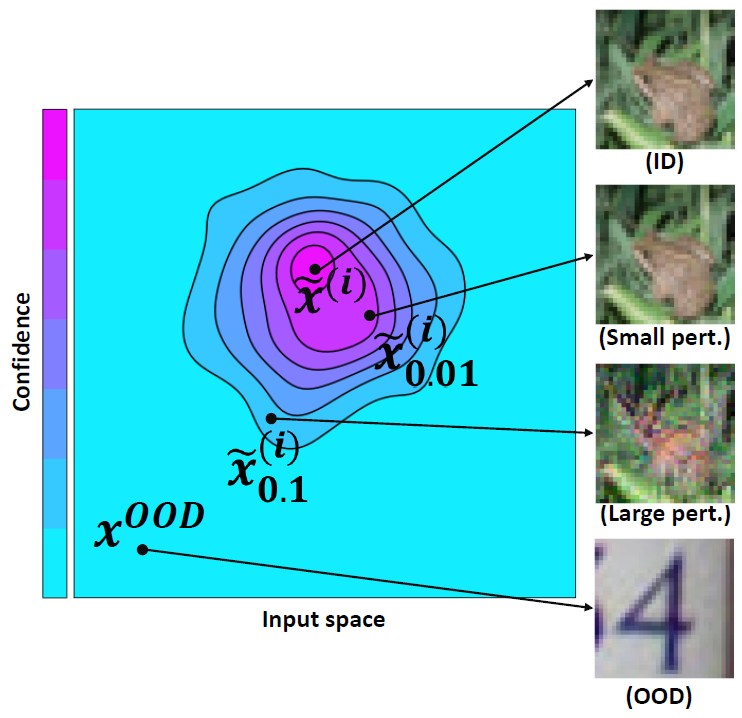
\includegraphics[width=0.36\textwidth]{sections/008_icml2021/eval/uncertainty_diagram.png}
\caption{Visualization of the desired uncertainty estimates. 
}
\label{fig:uncertainty_attack_diagram}
\end{figure}
%
DBU models have the advantage that they provide both, aleatoric uncertainty estimates resulting from irreducible uncertainty (e.g. class overlap or noise) and epistemic uncertainty estimates resulting from the lack of knowledge about unseen data (e.g. an unknown object is presented to the model). Both uncertainty types can be quantified from Dirichlet distributions using different uncertainty measures such as differential entropy, mutual information, or pseudo-counts. These uncertainty measures show outstanding performance in, e.g., the detection of OOD samples and thus are superior to softmax based confidence \citep{malini2018, reverse-kl, charpentier2020}.

Neural networks from the families outlined above are expected to \emph{know what they don't know}, i.e. they are supposed to notice when they are unsure about a prediction. 
This raises questions with regards to adversarial examples: should uncertainty estimation methods \emph{detect} these corrupted samples by indicating a high uncertainty on them and abstain from making a prediction? Or should uncertainty estimation be \emph{robust} to adversarial examples and assign the correct label even under perturbations? We argue that being robust to adversarial perturbations is the best option (see \cref{fig:uncertainty_attack_diagram}) for two reasons. First, in image classification a human is usually not able to observe any difference between an adversarial example and an unperturbed image. Second, the size of the perturbation corresponding to a good adversarial example is typically small w.r.t.\ the $L_p$-norm and thus assumed to be semantically meaningless. 
Importantly, robustness should not only be required for the class predictions, but also for the uncertainty estimates. This means that DBU models should be able to distinguish robustly between ID and OOD data even if those are perturbed. 
%Importantly, one should require robustness not only for the class predictions, but also for the uncertainty estimation. This means that DBU models should be able to distinguish robustly between ID and OOD data even if those are perturbed. 

In this chapter, we focus on DBU models and analyze their robustness capacity w.r.t. class predictions as well as uncertainty predictions. In doing so, we go beyond simple softmax output confidence by investigating advanced uncertainty measures such as differential entropy.
Specifically, we study the following questions: 
%
\begin{enumerate}
    \item \emph{Is low uncertainty a reliable indicator of correct predictions?}
    \item \emph{Can we use uncertainty estimates to detect label attacks on the class prediction?}
    \item \emph{Are uncertainty estimates such as differential entropy a robust feature for OOD detection?}
\end{enumerate}

In addressing these questions we place particular focus on adversarial perturbations of the input to evaluate the \emph{worst case} performance of the models on increasing complex data sets and attacks.
%
We evaluate robustness of DBU models w.r.t. to these three questions by comparing their performance on unperturbed and perturbed inputs. Perturbed inputs are obtained by computing \emph{label attacks} and \emph{uncertainty attacks}, which are a new type of attacks we propose.  While label attacks aim at changing the class prediction, uncertainty attacks aim at changing the uncertainty estimate such that ID data is marked as OOD data and vice versa.
%
In total, we performed more than $138,800$ attack settings to explore the robustness landscape of DBU models. Those settings cover different data sets, attack types, attack losses, attack radii, DBU model types and initialisation seeds.
%
Finally, we propose and evaluate median smoothing and adversarial training based on label attacks and uncertainty attacks to make DBU models more robust. Our median smoothing approach provides certificates on epistemic uncertainty measures such as differential entropy and allows to certify uncertainty estimation.  The code and further supplementary material is available online (\url{www.daml.in.tum.de/dbu-robustness}).





\section{Related work}
\label{sec:related_work}

% add papers not related to this work
The existence of adversarial examples is a problematic property of neural networks \citep{szegedy2014, goodfellow2014}. Previous works have study this phenomena by proposing adversarial attacks \citep{carlini2016, brendel2018,DBLP:conf/kdd/ZugnerAG18}, defenses \citep{cisse2017, gu2015} and verification techniques  \citep{wong2017, singh2019krelu, cohen2019, DBLP:conf/icml/BojchevskiKG20, kopetzki2021}. This includes the study of different settings such as i.i.d. inputs, sequential inputs and graphs \citep{zheng2016, DBLP:conf/nips/BojchevskiG19, cheng2020, schuchardt2021}.

% related work
In the context of uncertainty estimation, robustness of the class prediction has been studied in previous works for Bayesian Neural Networks \citep{blundell2015, osawa2019, wesley2019}, drop out \citep{drop_out} or ensembles \citep{ensemble_simple} focusing on data set shifts \cite{snoek2019} or adversarial attacks \cite{robustness_bnn, cardelli2019, wicker2020}. Despite their efficient and high quality uncertainty estimates, the robustness of DBU models has not been investigated in detail yet --- indeed only for one single DBU model, \citep{malinin2019} has briefly performed attacks aiming to change the label. 
In contrast, our work focuses on a large variety of DBU models and analyzes two robustness properties: robustness of the class prediction w.r.t. adversarial perturbations and robustness of uncertainty estimation w.r.t.\ our newly proposed attacks against uncertainty measures. 


This so called \emph{uncertainty attack} directly targets uncertainty estimation and are different from traditional \emph{label attacks}, which target the class prediction \citep{madry2018, raphael2020}. They allow us to jointly evaluate robustness of the class prediction and robustness of uncertainty estimation. This goes beyond previous attack defenses that were either focused on evaluating \emph{robustness w.r.t.\ class predictions} \citep{carlini2016, clever_robustness} or detecting attacks against the class prediction \citep{bypassing_attack_detection}. 


Different models have been proposed to account for uncertainty while being robust.  \citep{smith2018} and \citep{simple_ood_adv_detection} have tried to improve label attack detection based on uncertainty using drop-out or density estimation. In addition to improving label attack detection for large unseen perturbations, \citep{stutz2020} aimed at improving robustness w.r.t. class label predictions on small input perturbations. They used adversarial training and soft labels for adversarial samples further from the original input. \citep{qin2020} suggested a similar adversarial training procedure, that softens labels depending on the input robustness. These previous works consider the aleatoric uncertainty that is contained in the predicted categorical probabilities, but in contrast to DBU models they are not capable of taking epistemic uncertainty into account. 



Recently, four studies tried to obtain certificates on aleatoric uncertainty estimates. \citep{single_model_quantile} and \citep{confidence_certificate_rs} compute confidence intervals and certificates on softmax predictions. \citep{bitterwolf2020} uses interval bound propagation to compute bounds on softmax predictions within the $L_{\infty}$-ball around an OOD sample using ReLU networks. \citep{meinke2020} focuses on obtaining certifiably low confidence for OOD data. These four studies estimate confidence based on softmax predictions, which accounts for aleatoric uncertainty only. In this paper, we provide certificates which apply for all uncertainty measures. In particular, we use our certificates on epistemic uncertainty measures such as differential entropy which are well suited for OOD detection.



% List of Papers on Robustness (group website)
%
%Anna-Kathrin Kopetzki, Stephan Günnemann
%Reachable sets of classifiers and regression models: (non-)robustness analysis and robust training
%Machine Learning Journal, 2021 --> cited
%
%Jan Schuchardt, Aleksandar Bojchevski, Johannes Klicpera, Stephan Günnemann
%Collective Robustness Certificates: Exploiting Interdependence in Graph Neural Networks
%International Conference on Learning Representations (ICLR), 2021
%
%Simon Geisler, Daniel Zügner, Stephan Günnemann
%Reliable Graph Neural Networks via Robust Aggregation
%Neural Information Processing Systems (NeurIPS), 2020
%
%Aleksandar Bojchevski, Johannes Klicpera, Stephan Günnemann
%Efficient Robustness Certificates for Discrete Data: Sparsity-Aware Randomized Smoothing for Graphs, Images and More
%International Conference on Machine Learning (ICML), 2020
%
%Daniel Zügner, Stephan Günnemann
%Certifiable Robustness of Graph Convolutional Networks under Structure Perturbations
%ACM SIGKDD Conference on Knowledge Discovery and Data Mining (KDD), 2020
%
%Daniel Zügner, Oliver Borchert, Amir Akbarnejad, Stephan Günnemann
%Adversarial Attacks on Graph Neural Networks: Perturbations and their Patterns
%ACM Transactions on Knowledge Discovery from Data, 2020
%
%Aleksandar Bojchevski, Stephan Günnemann
%Certifiable Robustness to Graph Perturbations
%Neural Information Processing Systems (NeurIPS), 2019
%
%Daniel Zügner, Stephan Günnemann
%Certifiable Robustness and Robust Training for Graph Convolutional Networks
%ACM SIGKDD Conference on Knowledge Discovery and Data Mining (KDD), 2019
%
%Aleksandar Bojchevski, Stephan Günnemann
%Adversarial Attacks on Node Embeddings via Graph Poisoning
%International Conference on Machine Learning (ICML), 2019
%
%Daniel Zügner, Stephan Günnemann
%Adversarial Attacks on Graph Neural Networks via Meta Learning
%International Conference on Learning Representations (ICLR), 2019
%
%Daniel Zügner, Amir Akbarnejad, Stephan Günnemann
%Adversarial Attacks on Neural Networks for Graph Data (Extended Abstract)
%International Joint Conference on Artificial Intelligence (IJCAI), 2019
%(Invited contribution to the IJCAI Sister Conference Best Paper Track)
%
%Daniel Zügner, Amir Akbarnejad, Stephan Günnemann
%Adversarial Attacks on Neural Networks for Graph Data 
%(Best Research Paper Award)
%ACM SIGKDD Conference on Knowledge Discovery and Data Mining (KDD), 2018
%
%
%Richard Leibrandt, Stephan Günnemann
%Making Kernel Density Estimation Robust towards Missing Values in Highly Incomplete Multivariate Data without Imputation
%SIAM International Conference on Data Mining (SDM), 2018 
%
%Aleksandar Bojchevski, Stephan Günnemann
%Bayesian Robust Attributed Graph Clustering: Joint Learning of Partial Anomalies and Group Structure
%AAAI Conference on Artificial Intelligence, pp. 2738-2745, 2018
%
%Aleksandar Bojchevski, Yves Matkovic, Stephan Günnemann
%Robust Spectral Clustering for Noisy Data: Modeling Sparse Corruptions Improves Latent Embeddings
%ACM SIGKDD Conference on Knowledge Discovery and Data Mining (KDD), pp. 737-746, 2017


\section{Dirichlet-based uncertainty models}
\label{sec:dirichlet_models}
%
Standard (softmax) neural networks predict the parameters of a categorical distribution \smash{$\vp\dataix = [p\dataix_1, \ldots, p\dataix_\nclass]$} for a given input \smash{$\x\dataix \in \mathbb{R}^{d}$}, where $\nclass$ is the number of classes. 
Given the parameters of a categorical distribution, the \emph{ aleatoric uncertainty} can be evaluated. The aleatoric uncertainty is the uncertainty on the class label prediction \smash{$y\dataix \in \{1, \ldots, \nclass\}$}. For example if we predict the outcome of an unbiased coin flip, the model is expected to have high aleatoric uncertainty and predict $p(\text{head})=0.5$.

\begin{table*}[ht]
	\centering
	\caption{Summary of DBU models. Further details on the loss functions are provided in the appendix.}
	\label{tab:dirichlet_models}
	\resizebox{.9 \textwidth}{!}{%
		\begin{tabular}{lllllll}
			\toprule
			{} &  \textbf{$\alpha\dataix$-parametrization} & \textbf{Loss} & \textbf{OOD training data} & \textbf{Ensemble training} & \textbf{Density estimation}\\
			\midrule
			\textbf{\PostNet} & $f_{\theta}(\x\dataix) = \mathbf{1} + \bm{\alpha}\dataix$ & Bayesian loss & No & No & Yes \\
			\textbf{\PriorNet} & $f_{\theta}(\x\dataix) = \bm{\alpha}\dataix$ & Reverse KL & Yes &  No & No \\
			\textbf{\DDNet} & $f_{\theta}(\x\dataix) = \bm{\alpha}\dataix$ & Dir. Likelihood & No & Yes & No \\
			\textbf{\EvNet} & $f_{\theta}(\x\dataix) =  \mathbf{1} + \bm{\alpha}\dataix$ & Expected MSE & No &  No & No \\
			\bottomrule
		\end{tabular}
	}
	%\vspace{-.5cm}
\end{table*}


In contrast to standard (softmax) neural networks, DBU models predict the parameters of a Dirichlet distribution -- the natural prior of categorical distributions -- given input~$\x \dataix$ (i.e. \smash{$q\dataix = \text{Dir}(\bm{\alpha}\dataix)$} where \smash{$f_{\theta}(\x\dataix) = \bm{\alpha} \dataix \in \mathbb{R}_+^\nclass$}). Hence, the \emph{epistemic distribution} \smash{$q\dataix$} expresses the \emph{epistemic} uncertainty on $\x \dataix$, i.e. the uncertainty on the categorical distribution prediction \smash{$\vp\dataix$}. From the epistemic distribution, follows an estimate of the \emph{aleatoric distribution} of the class label prediction $\text{Cat}(\bar{\vp}\dataix)$ where \smash{$\E_{q\dataix}[\vp\dataix] = \bar{\vp}\dataix$}.
An advantage of DBU models is that one pass through the neural network is sufficient to compute epistemic distribution, aleatoric distribution, and predict the class label:
%
\begin{equation}
\begin{aligned}
    q^{(\idata)}           = \text{Dir}(\bm{\alpha}\dataix), \hspace{5pt}
    \bar{p}_\iclass\dataix  = \frac{\alpha_\iclass\dataix}{\alpha_0\dataix}, \hspace{5pt}
    y^{(\idata)}           = \arg \max_{\iclass} \;[\bar{p}_\iclass\dataix]
\end{aligned}
\end{equation}
%
where $\alpha_0\dataix = \sum^{\nclass}_{\iclass=1} \alpha_\iclass\dataix$. This parametrization allows to compute classic uncertainty measures in closed-form such as the total pseudo-count $m\dataix_{\alpha_0} = \sum_\iclass \alpha\dataix_\iclass$, the differential entropy of the Dirichlet distribution $m\dataix_\text{diffE} = h(\text{Dir}(\bm{\alpha}\dataix))$ or the mutual information $m\dataix_\text{MI} = I(y\dataix, \vp\dataix)$ (App. \ref{subsec:appendix_measurecomp}, \citep{malini2018}). 
Hence, these measure can efficiently be used to assign high uncertainty to unknown data, which makes DBU models specifically suited for detection of OOD samples. 





Several recently proposed models for uncertainty estimations belong to the family of DBU models, such as \PriorNet, \EvNet, \DDNet and \PostNet. These models differ in terms of their parametrization of the Dirichlet distribution, the training, and density estimation. An overview of theses differences is provided in Table \ref{tab:dirichlet_models}. In our study we evaluate all recent versions of these models.


Contrary to the other models, Prior Networks \textbf{(\PriorNet)} \citep{malini2018, malinin2019}  require OOD data for training to ``teach'' the neural network the difference between ID and OOD data. \PriorNet is trained with a loss function consisting of two KL-divergence terms. The fist term is designed to learn Dirichlet parameters for ID data, while the second one is used to learn a flat Dirichlet distribution %($\boldsymbol{\alpha} = \boldsymbol{1}$) 
for OOD data: 
%
\begin{equation}
\begin{aligned}
    L_{\mathrm{\PriorNet}} &= \frac{1}{N} \left[\sum_{\x\dataix \in \text{ID data}}  [\mathrm{KL} [\mathrm{Dir} (\alpha^{\mathrm{ID}}) || q\dataix]]  \right. \\
                           &+ \left.\sum_{\x\dataix \in OOD data} [\mathrm{KL} [\mathrm{Dir} (\alpha^{\mathrm{OOD}}) || q\dataix]]\right] \\
\end{aligned}
\end{equation}
%
where $\alpha^{\mathrm{ID}}$ and $\alpha^{\mathrm{OOD}}$ are hyper-parameters. Usually $\alpha^{\mathrm{ID}}$ is set to $1e^{1}$ for the correct class and $1$ for all other classes, while $\alpha^{\mathrm{OOD}}$ is set to $\mathbf{1}$ for all classes.
%
There a two variants of \PriorNet. The first one is trained based on reverse KL-divergence \citep{malinin2019}, while the second one is trained with KL-divergence \citep{malini2018}. In our experiments, we include the most recent reverse version of \PriorNet, as it shows superior performance \citep{malinin2019}. 

Evidential Networks \textbf{(\EvNet)} \citep{sensoy2018} are trained with a loss that computes the sum of squares between the on-hot encoded true label $\vy*\dataix$ and the predicted categorical $\vp\dataix$ under the Dirichlet distribution:
%
\begin{equation}
\begin{aligned}
    L_{\mathrm{\EvNet}} &= \frac{1}{N} \sum_i \E_{\vp\dataix \sim \text{Dir}(\bm{\alpha}\dataix)}||\vy*\dataix - \vp\dataix||^2 \\
\end{aligned}
\end{equation}

Ensemble Distribution Distillation \textbf{(\DDNet)} \citep{malinin2019ensemble} is trained in two steps. First, an ensemble of $M$ classic neural networks needs to be trained. 
Then, the soft-labels \smash{$\{\vp_{m}\dataix\}_{m=1}^{M}$} provided by the ensemble of networks are distilled into a Dirichlet-based network by fitting them with the maximum likelihood under the Dirichlet distribution: 
\begin{equation}
\begin{aligned}
    L_{\mathrm{\DDNet}} &= - \frac{1}{N}  \sum_i \sum_{m=1}^{M} [\ln q\dataix(\pi^{im})] \\
\end{aligned}
\end{equation}
where $\pi^{im}$ denotes the soft-label of $m$th neural network. 

Posterior Network \textbf{(\PostNet)} \citep{charpentier2020} performs density estimation for ID data with normalizing flows and uses a Bayesian loss formulation: %composed of the Uncertain Cross-Entropy loss \citep{uncertainty_time} and an entropy regularizer inspired by Bayesian theory.
\begin{equation}
\begin{aligned}
    L_{\mathrm{\PostNet}} &= \frac{1}{N} \sum_i \E_{q(p\dataix)}  [\mathrm{CE} (p\dataix, y\dataix)] - H(q\dataix)
\end{aligned}
\end{equation}
where $\mathrm{CE}$ denotes the cross-entropy.
%
All loss functions can be computed in closed-form. For more details please have a look at the original paper on \PriorNet \citep{malini2018}, \PostNet \citep{charpentier2020}, \DDNet \citep{malinin2019} and \EvNet \citep{sensoy2018}.
Note that \EvNet and \PostNet model the Dirichlet parameters as \smash{$f_{\theta}(\x\dataix) = 1 + \bm{\alpha}\dataix$} while \PriorNet, \RevPriorNet and \DDNet compute them as \smash{$f_{\theta}(\x\dataix) = \bm{\alpha}\dataix$}. 









\section{Robustness of Dirichlet-based uncertainty models}
\label{sec:attack_dirichlet_model}

We analyze robustness of DBU models on tasks in connection with uncertainty estimation w.r.t.\ the following four aspects: \emph{accuracy}, \emph{confidence calibration}, \emph{label attack detection} and \emph{OOD detection}. Uncertainty is quantified by differential entropy, mutual information or pseudo counts. 
A formal definition of all uncertainty estimation measures is provided in the appendix (see Section~\ref{subsec:appendix_measurecomp}).  

Robustness of Dirichlet-based uncertainty models is evaluated based on \emph{label attacks} and a newly proposed type of attacks called \emph{uncertainty attacks}. 
While label attacks aim at changing the predicted class, uncertainty attacks aim at changing the uncertainty assigned to a prediction. 
All previous works are based on label attacks and focus on robustness w.r.t. the class prediction. Thus, we are the first to propose attacks targeting uncertainty estimates such as differential entropy and analyze desirable robustness properties of DBU models beyond the class prediction. 
Label attacks and uncertainty attacks both compute a perturbed input $\tilde{\x}\dataix$ close to the original input~$\x\dataix$ i.e. $|| \x\dataix - \tilde{\x}\dataix ||_2 < r$ where $r$ is the attack radius. This perturbed input is obtained by optimizing a loss function $l(\x)$ using Fast Gradient Sign Method (FGSM) or Projected Gradient Descent (PGD). Furthermore, we include a black box attack setting (Noise) which generates 10 noise samples from a Gaussian distribution, which is centered at the original input. From these 10 perturbed samples we choose the one with the greatest effect on the loss function and use it as attack. 
To complement attacks, we compute certificates on uncertainty estimates using median smoothing \cite{median_smoothing}. 


%Reviewer: avoid redundancy within assessment metric paragraphs, explain high level + differences
The following questions we address by our experiments have a common assessment metric and can be treated as binary classification problems: distinguishing between correctly and wrongly classified samples, discriminating between non-attacked input and attacked inputs or differentiating between ID data and OOD data. To quantify the performance of the models on these binary classification problems, we compute the area under the precision recall curve (AUC-PR).

Experiments are performed on two image data sets (MNIST \citep{mnist} and CIFAR10 \citep{cifar10}), which contain bounded inputs and two tabular data sets (Segment \citep{uci_datasets} and Sensorless drive \citep{uci_datasets}), consisting of unbounded inputs. Note that unbounded inputs are challenging since it is impossible to describe the infinitely large OOD distribution. As PriorNet requires OOD training data, we use two further image data sets (FashionMNIST \citep{fashionmnist} and CIFAR100 \citep{cifar10}) for training on MNIST and CIFAR10, respectively. All other models are trained without OOD data. To obtain OOD data for the tabular data sets, we remove classes from the ID data set (class window for the Segment data set and class 9 for Sensorless drive) and use them as the OOD data. Further details on the experimental setup are provided in the appendix (see Section~\ref{subsec:exp_setup}).



 


\subsection{Uncertainty estimation under label attacks}
\label{subsec:label_attacks}
%
Label attacks aim at changing the predicted class. To obtain a perturbed input with a different label, we maximize the cross-entropy loss $\tilde{\x}\dataix \approx \arg\max_{\x} l(\x) = \text{CE}(\vp\dataix, \vy\dataix)$ under the radius constraint. For the sake of completeness we additionally analyze label attacks w.r.t. to their performance of changing the class prediction and the accuracy of the neural network under label attacks constraint by different radii (see Appendix, Table~\ref{tab:acc_label_attack}). As expected and partially shown by previous works, none of the DBU models is robust against label attacks. %, neither on the image data sets nor on the tabular data sets.
However, we note that \PriorNet is slightly more robust than the other DBU models. This might be explained by the use of OOD data during training, which can be seen as some kind of robust training. 
%
From now on, we switch to the core focus of this work and analyze robustness properties of uncertainty estimation. 




\begin{table*}[ht]
	\centering
	\caption{Distinguishing between correctly predicted and wrongly predicted labels based on the differential entropy under PGD label attacks (metric: AUC-PR).}
	%\begin{small}
	\resizebox{0.8\textwidth}{!}{
		\begin{tabular}{@{}rrrrrrrc|crrrrrr@{}}
			\toprule
			& \multicolumn{6}{c}{CIFAR10} & & & \multicolumn{6}{c}{Sensorless} \\
			\cmidrule{2-7}  \cmidrule{10-15}
			Att. Rad. & 0.0 & 0.1 & 0.2 & 0.5 & 1.0 & 2.0 & & & 0.0 & 0.1 & 0.2 & 0.5 & 1.0 & 2.0  \\
			\midrule
			%& \multicolumn{7}{c}{MNIST} & & & \multicolumn{7}{c}{CIFAR10} \\
			\PostNet  &  \bf{98.7} &  88.6 &  56.2 &   7.8 &   1.2 &   0.4 &  & %0.3 & & 
			&  99.7 &   8.3 &   3.9 &  3.6 &  \bf{7.0} &  \bf{9.8} \\%&  \bf{11.3} \\
			\PriorNet &  92.9 &  77.7 &  60.5 &  \bf{37.6} &  \bf{24.9} &  \bf{11.3} &  & %\bf{3.0} & & 
			&  99.8 &  10.5 &   3.2 &  0.7 &  0.2 &  0.2 \\%&   2.2 \\ 
			\DDNet    &  97.6 &  \bf{91.8} &  \bf{78.3} &  18.1 &   0.8 &   0.0 &  &%0.0 & &
			&  99.7 &  11.9 &   1.6 &  0.4 &  0.2 &  0.1 \\%&   0.2 \\ 
			\EvNet    &  97.9 &  85.9 &  57.2 &  10.2 &   4.0 &   2.4 &  &%0.3 & & 
			&  \bf{99.9} &  \bf{22.9} &  \bf{13.0} &  \bf{6.0} &  3.7 &  3.2 \\%&   3.1 \\
			\bottomrule
		\end{tabular}}
	%\end{small}
	\label{tab:conf_label_attack}
\end{table*}







\textbf{Is low uncertainty a reliable indicator of correct predictions?} \\
%
\underline{\emph{Expected behavior:}}  Predictions with low uncertainty are more likely to be correct than high uncertainty predictions. 
\underline{\emph{Assessment metric:}} We distinguish between correctly classified samples (label 0) and wrongly classified ones (label 1) based on the differential entropy scores produced by the DBU models \citep{malini2018}. Correctly classified samples are expected to have low differential entropy, reflecting the model's confidence, and analogously wrongly predicted samples are expected to have higher differential entropy. 
%\dz{State that the metric is AUC-PR?} 
\underline{\emph{Observed behavior:}} Note that the positive and negative class are not balanced, thus, the use of AUC-PR scores \citep{imbalance_apr} are important to enable meaningful measures. While uncertainty estimates are indeed an indicator of correctly classified samples on unperturbed data, none of the models maintains its high performance on perturbed data computed by PGD, FGSM or Noise label attacks (see. Table~\ref{tab:conf_label_attack}, \ref{tab:conf_label_attack_fgsm} and \ref{tab:conf_label_attack_noise_attack}). Thus, using uncertainty estimates as indicator for correctly labeled inputs is not robust to adversarial perturbations. This result is notable, since the used attacks do not target uncertainty. 





\vspace{1em}
\begin{table*}[ht]
	\centering
	\caption{Label Attack-Detection by normally trained DBU models based on differential entropy under PGD label attacks (AUC-PR).}
	%\begin{small}
	\resizebox{0.8\textwidth}{!}{
		\begin{tabular}{@{}rrrrrrc|crrrrr@{}}
			\toprule
			& \multicolumn{5}{c}{CIFAR10} & & & \multicolumn{5}{c}{Sensorless} \\
			\cmidrule{2-6}  \cmidrule{9-13}
			Att. Rad. & 0.1 & 0.2 & 0.5 & 1.0 & 2.0 & & & 0.1 & 0.2 & 0.5 & 1.0 & 2.0 \\
			\midrule
			\PostNet  &  \bf{63.4} &  \bf{66.9} &  42.1 &  32.9 &  31.6 &  &%31.2 & & 
			&  47.7 &  42.3 &  36.9 &  \bf{48.5} &  \bf{85.0} \\%&  \bf{99.0} \\ 
			\PriorNet &  53.3 &  56.0 &  55.6 &  \bf{49.2} &  42.2 & &%  35.4 & & 
			&  38.8 &  33.6 &  31.4 &  33.1 &  40.9 \\%&  53.5 \\ 
			\DDNet    &  55.8 &  60.5 &  \bf{57.3} &  38.7 &  32.3 & &% 31.4 & & 
			&  \bf{53.5} &  42.2 &  35.0 &  32.8 &  32.6 \\%&  33.9 \\ 
			\EvNet    &  48.4 &  46.9 &  46.3 &  46.3 &  \bf{44.5} & &% \bf{42.5} & &
			&  48.2 &  \bf{42.6} &  \bf{38.2} &  36.0 &  37.2 \\%&  41.7 \\
			\bottomrule 			
		\end{tabular}}
	%\end{small}
	\label{tab:label_attack_detect}
\end{table*}








%\vspace{-0.5em}
\textbf{Can uncertainty estimates be used to detect label attacks against the class prediction?}\\
%
\underline{\emph{Expected behavior:}} Adversarial examples are not from the natural data distribution. Therefore, DBU models are expected to detect them as OOD data by assigning them a higher uncertainty. We expect that perturbations computed based on a bigger attack radius~$r$ are easier to detect as their distance from the data distribution is larger. 
\underline{\emph{Assessment metric:}} The goal of attack-detection is to distinguish between unperturbed samples (label 0) and perturbed samples (label 1). Uncertainty on samples is quantified by the differential uncertainty \citep{malini2018}. Unperturbed samples are expected to have low differential entropy, because they are from the same distribution as the training data, while perturbed samples are expected to have a high differential entropy. 
%Further results based on other uncertainty measures are provided in the appendix. 
\underline{\emph{Observed behavior:}} Table~\ref{tab:acc_label_attack} shows that the accuracy of all models decreases significantly under PGD label attacks, but none of the models is able to provide an equivalently increasing attack detection rate (see Table~\ref{tab:label_attack_detect}). Even larger perturbations are hard to detect for DBU models. 

Similar results are obtained when we use mutual information or the precision~$\alpha_0$ to quantify uncertainty (see appendix Table~\ref{tab:conf_label_attack_mi} and~\ref{tab:conf_label_attack_alpha}).
Although PGD label attacks do not explicitly consider uncertainty, they seem to generate adversarial examples with similar uncertainty as the original input. 
Such high-certainty adversarial examples are illustrated in Figure~\ref{fig:attaked_samples_labels}, where certainty is visualized based on the precision~$\alpha_0$, which is supposed to be high for ID data and low for OOD data. While the original input (perturbation size $0.0$) is correctly classified as frog and ID data, there exist adversarial examples that are classified as deer or bird. The certainty ($\alpha_0$-score) on the prediction of these adversarial examples has a similar or even higher value than on the prediction of the original input. Using the differential entropy to distinguish between ID and OOD data results in the same ID/OOD assignment since the differential entropy of the three right-most adversarial examples is similar or even smaller than on the unperturbed input. 







Under the less powerful FGSM and Noise attacks (see Appendix), DBU models achieve mostly higher attack detection rates than under PGD attacks. This suggests that uncertainty estimation is able to detect weak attacks, which is consistent with the observations in \citep{malinin2018_adetect} but fails under stronger PGD attacks. 
%
\begin{figure}[ht]
	\centering
	\resizebox{0.42\textwidth}{!}{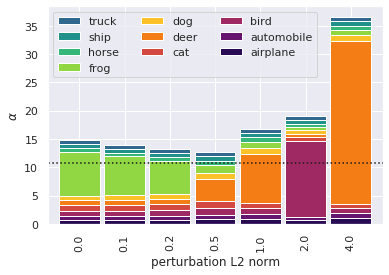
\includegraphics[width=\textwidth]{sections/008_icml2021/eval/ddnet_label_id_cifar10_alphas.png}}%
	\resizebox{0.42\textwidth}{!}{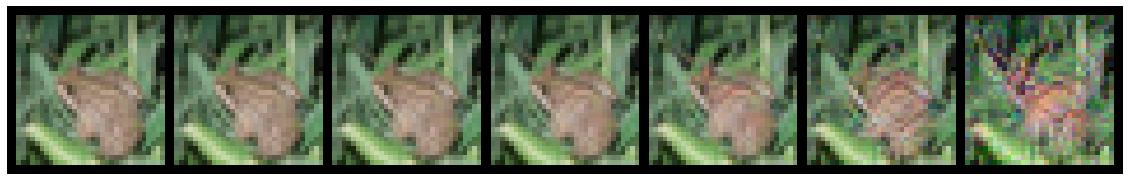
\includegraphics[width=\textwidth]{sections/008_icml2021/eval/ddnet_label_id_cifar10_images.png}}
	\caption{Input and predicted Dirichlet-parameters under label attacks (dotted line: threshold to distinguish ID and OOD data). % based on the precision~$\alpha_0$.
		%-14.2216765174
		%0.0 [-17.875761]
		%0.1 [-17.257824]
		%0.2 [-16.648003]
		%0.5 [-15.014889]
		%1.0 [-17.504786]
		%2.0 [-22.63896]
		%4.0 [-24.941536]
	}
	\label{fig:attaked_samples_labels}
\end{figure}


On tabular data sets, \PostNet shows a better label attack detection rate for large perturbations. This observation might be explained by the fact that the density estimation of the ID samples has been shown to work better for tabular data sets \citep{charpentier2020}. 
%
Overall, none of the DBU models provides a reliable indicator for adversarial inputs that target the class prediction. 





\vspace{.4mm}
\begin{table*}[ht]
	\centering
	\caption{OOD detection based on differential entropy under PGD uncertainty attacks against differential entropy computed on ID data and OOD data (metric: AUC-PR).}
%	\begin{small}
	\resizebox{\textwidth}{!}{
		\begin{tabular}{@{}rrrrrrrc|crrrrrr@{}}
			\toprule
			& \multicolumn{6}{c}{ID-Attack (non-attacked OOD)} &  & &  \multicolumn{6}{c}{OOD-Attack (non-attacked ID)} \\
			\cmidrule{2-7}  \cmidrule{10-15}
			Att. Rad. & 0.0 & 0.1 & 0.2 & 0.5 & 1.0 & 2.0 & & &
			0.0 & 0.1 & 0.2 & 0.5 & 1.0 & 2.0  \\
			\midrule
			& \multicolumn{14}{c}{\textbf{CIFAR10 -- SVHN}} \\
			\PostNet  &  81.8 &  64.3 &  47.2 &  22.4 &  17.6 &  \bf{16.9} &  &%\bf{16.4} & &
			&  81.8 &  60.5 &  40.7 &  23.3 &  21.8 &  19.8 \\%&  18.1 \\ 
			\PriorNet &  54.4 &  40.1 &  30.0 &  17.9 &  15.6 &  15.4 &  &%15.4 & &
			&  54.4 &  40.7 &  30.7 &  19.5 &  16.5 &  15.7 \\%&  15.4 \\
			\DDNet    &  \bf{82.8} &  \bf{71.4} &  \bf{59.2} &  \bf{28.9} &  16.0 &  15.4 & &% 15.4 & &
			&  \bf{82.8} &  \bf{72.0} &  \bf{57.2} &  20.8 &  15.6 &  15.4 \\%&  15.4 \\
			\EvNet    &  80.3 &  62.4 &  45.4 &  21.7 &  \bf{17.9} &  16.5 &  &%15.6 & &
			&  80.3 &  58.2 &  46.5 &  \bf{34.6} &  \bf{28.0} &  \bf{23.9} \\%&  \bf{21.0} \\
			\midrule
			& \multicolumn{14}{c}{\textbf{Sens. -- Sens. class 10, 11}} \\
			\PostNet  &  \bf{74.5} &  \bf{39.8} &  \bf{36.1} &  \bf{36.0} &  \bf{45.9} &  \bf{46.0} & &% \bf{46.0} & &
			&  \bf{74.5} &  \bf{43.3} &  \bf{42.0} &  \bf{32.1} &  \bf{35.1} &  \bf{82.6} \\%&  \bf{99.4} \\
			\PriorNet &  32.3 &  26.6 &  26.5 &  26.5 &  26.6 &  28.3 & &% 38.6 & &
			&  32.3 &  26.7 &  26.6 &  26.6 &  27.0 &  30.4 \\%&  36.8 \\ 
			\DDNet    &  31.7 &  26.8 &  26.6 &  26.5 &  26.6 &  27.1 & &% 30.5 & &
			&  31.7 &  27.1 &  26.7 &  26.7 &  26.8 &  26.9 \\%&  27.3 \\ 
			\EvNet    &  66.5 &  30.5 &  28.2 &  27.1 &  28.1 &  31.8 & &% 37.5 & &
			&  66.5 &  38.7 &  36.1 &  30.2 &  28.2 &  28.8 \\%&  32.2 \\
			\bottomrule
		\end{tabular}}
%	\end{small}
	\label{tab:id_ood_attacks}
\end{table*}









\subsection{Attacking uncertainty estimation}
\label{subsec:uncertainty_attacks}

DBU models are designed to provide sophisticated uncertainty estimates (beyond softmax scores) alongside predictions and use them to detect OOD samples. In this section, we propose and analyze a new attack type that targets these uncertainty estimates. 
DBU models enable us to compute uncertainty measures i.e. differential entropy, mutual information and precision~$\alpha_0$ in closed from (see \citep{malini2018} for a derivation). Uncertainty attacks use this closed form solution as loss function for PGD, FGSM or Noise attacks. 
Since differential entropy is the most widely used metric for ID-OOD-differentiation, we present results based on the differential entropy loss function $\tilde{\x}\dataix \approx \arg\max_{\x} l(\x) = \text{Diff-E}(\text{Dir}(\mathbf{\alpha}\dataix))$: 
%
\begin{equation}
\begin{aligned}
	\text{Diff-E}(\text{Dir}(\mathbf{\alpha}\dataix))  = &\sum_c^K \ln \Gamma (\alpha_c^{(i)}) - \ln \Gamma (\alpha_0^{(i)}) \\
	&- \sum_c^K (\alpha_c^{(i)} -1) \cdot (\Psi (\alpha_c^{(i)}) - \Psi (\alpha_0^{(i)}))
\end{aligned}
\end{equation}
%
where $\alpha_0^{(i)} = \sum_c \alpha_c^{(i)}$. 
Result based on further uncertainty measures, loss functions and more details on attacks are provided in the appendix. 


We analyze the performance of DBU models under uncertainty attacks w.r.t.\ two tasks. First, uncertainty attacks are computed on ID data aiming to indicate it as OOD data, while OOD data is left non-attacked. Second, we attack OOD data aiming to indicate it as ID data, while ID data is not attacked. Hence, uncertainty attacks target at posing ID data as OOD data and vice versa.


\begin{figure}[ht!]
    \centering
        \begin{subfigure}[t]{0.49\columnwidth}
        \centering
        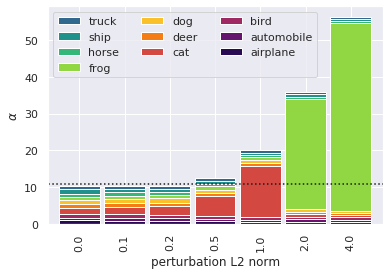
\includegraphics[width=0.99 \textwidth]{sections/008_icml2021/eval/ddnet_unc_ood_cifar10_alphas.png}
    \end{subfigure}%
    \begin{subfigure}[t]{0.49\columnwidth}
        \centering
        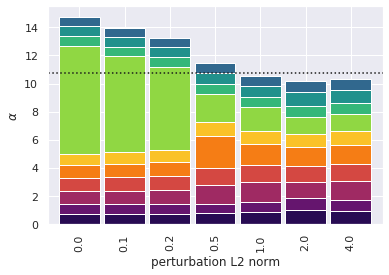
\includegraphics[width=0.99 \textwidth]{sections/008_icml2021/eval/ddnet_unc_id_cifar10_alphas.png}
    \end{subfigure}%


    \begin{subfigure}[t]{0.49 \columnwidth}
        \centering
        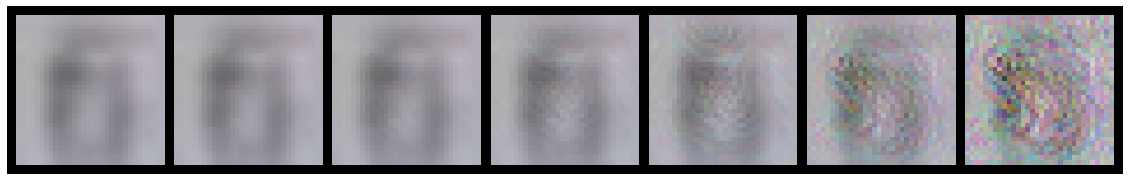
\includegraphics[width=0.99 \textwidth]{sections/008_icml2021/eval/ddnet_unc_ood_cifar10_images.png}
        \caption{OOD uncertainty attack
        %-14.2216765174
        %0.0 [-13.115507]
        %0.1 [-13.353642]
        %0.2 [-13.723262]
        %0.5 [-16.341246]
        %1.0 [-22.298155]
        %2.0 [-28.071136]
        %4.0 [-33.148224]
        }
        \label{fig:attaked_samples_idood_a}
    \end{subfigure}%
        \begin{subfigure}[t]{0.49 \columnwidth}
        \centering
        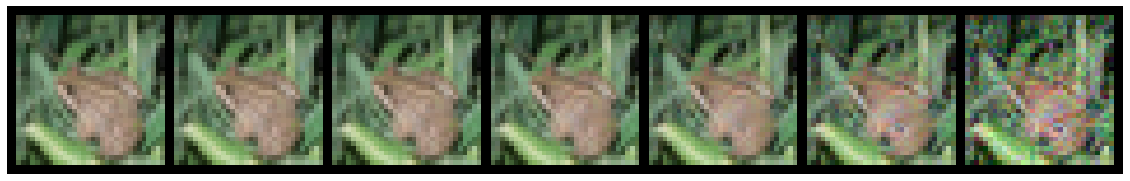
\includegraphics[width=0.99 \textwidth]{sections/008_icml2021/eval/ddnet_unc_id_cifar10_images.png}
        \caption{ID uncertainty attack
        %-14.2216765174
        %0.0 [-17.875761]
        %0.1 [-17.256058]
        %0.2 [-16.65203]
        %0.5 [-14.321844]
        %1.0 [-13.6354265]
        %2.0 [-13.046129]
        %4.0 [-13.1426115]
        }
        \label{fig:attaked_samples_idood_b}
    \end{subfigure}%
    \caption{ID and OOD input with corresponding Dirichlet-parameters under uncertainty attacks (dotted line: threshold to distinguish ID and OOD).}
    \label{fig:attaked_samples_idood}
	%\vspace{-.5cm}
\end{figure}





\textbf{Are uncertainty estimates a robust feature for OOD detection?}\\
%
\underline{\emph{Expected behavior:}} We expect DBU models to be able to distinguish between ID and OOD data by providing reliable uncertainty estimates, even under small perturbations. Thus, we expect uncertainty estimates of DBU models to be robust under attacks. 
%
\underline{\emph{Assessment metric:}} We distinguish between ID data (label 0) and OOD data (label 1) based on the differential entropy as uncertainty scoring function \citep{malini2018}. Differential entropy is expected to be small on ID samples and high on OOD samples. Experiments on further uncertainty measure and results on the AUROC metric are provided in the appendix. 
%
\underline{\emph{Observed behavior:}} OOD samples are perturbed as illustrated in  Figure~\ref{fig:attaked_samples_idood}. Part (a) of the figure illustrates an OOD-samples, that is correctly identified as OOD. Adding adversarial perturbations $\geq 0.5$ changes the Dirichlet parameters such that the resulting images are identified as ID, based on precision or differential entropy as uncertainty measure. Perturbing an ID sample (part (b)) results in images that are marked as OOD samples. 
OOD detection performance of all DBU models rapidly decreases with the size of the perturbation, regardless of whether attacks are computed on ID or OOD data (see Table~\ref{tab:id_ood_attacks}). This performance decrease is also observed with AUROC as metric, attacks based on FGSM, Noise, when we use mutual information or precision~$\alpha_0$ to distinguish between ID samples and OOD samples (see appendix Table~\ref{tab:id_ood_attacks_part2} - \ref{tab:id_ood_attacks_measure_diffE_aupr_noise}). 
Thus, using uncertainty estimation to distinguish between ID and OOD data is not robust. 








\begin{table*}[ht!]
	\centering
	%\begin{tiny}
	\resizebox{\textwidth}{!}{ %0.866
%    \begin{tabular}{lccccccc}
%    \toprule
 %   \textbf{Att. Rad.} & 0.0 &   0.1 &  0.2 &  0.5 &  1.0 &  2.0 \\
 %   \midrule
  %  & \multicolumn{6}{c}{\textbf{Smoothed models}} \\
%    \input{tables_v2/normal-cifar10-in-PGD_L2-crossentropy-confidence}
%    \midrule
%    & \multicolumn{6}{c}{\textbf{Smoothed models + adversarial training using label attacks}} \\
%    \input{tables_v2/adv-cifar10-in-PGD_L2-crossentropy-confidence}
%    \midrule
%    & \multicolumn{6}{c}{\textbf{Smoothed models + adversarial training using uncertainty attacks}} \\
%    \input{tables_v2/unc_adv-cifar10-in-PGD_L2-crossentropy-confidence}
%    \bottomrule
%    \end{tabular}
    \begin{tabular}{clccccccc}
    \toprule
    & \textbf{Att. Rad.} & 0.0 &   0.1 &  0.2 &  0.5 &  1.0 &  2.0 \\
    \midrule
    %& & \multicolumn{6}{c}{\textbf{Smoothed models}} \\
      \multirow{4}{1.2cm}{Smoothed models} & \textbf{PostNet} &  $80.5\cdot\bm{{\color{black}91.5}}\cdot94.5$ &  
  $52.8\cdot\bm{{\color{black}71.6}}\cdot95.2$ &  
  $31.9\cdot\bm{{\color{black}51.0}}\cdot96.8$ &  
  $\phantom{0}5.6\cdot\bm{{\color{blue}11.7}}\cdot100.0$ &  
  $\phantom{0}0.3\cdot\bm{{\color{black}\phantom{0}0.6}}\cdot100.0$ &  
  $\phantom{0}0.0\cdot\bm{{\color{black}\phantom{0}0.0}}\cdot100.0$ \\
 & \textbf{PriorNet} &  
 $81.9\cdot\bm{{\color{black}86.8}}\cdot88.0$ &     
 $69.6\cdot\bm{{\color{blue}78.0}}\cdot90.1$ &     
 $50.9\cdot\bm{{\color{blue}65.8}}\cdot89.4$ & 
 $36.5\cdot\bm{{\color{blue}59.9}}\cdot\phantom{0}97.0$ &   
 $24.3\cdot\bm{{\color{blue}39.3}}\cdot100.0$ &    
 $\phantom{0}9.2\cdot\bm{{\color{blue}17.9}}\cdot100.0$ \\
  &   \textbf{DDNet} &  
  $65.9\cdot\bm{{\color{black}81.2}}\cdot83.0$ &  
  $55.8\cdot\bm{{\color{black}70.5}}\cdot87.2$ &  
  $37.8\cdot\bm{{\color{black}56.8}}\cdot88.1$ &  
  $10.1\cdot\bm{{\color{blue}21.9}}\cdot\phantom{0}94.3$ &      
  $\phantom{0}0.9\cdot\phantom{0}\bm{{\color{blue}1.6}}\cdot\phantom{0}99.6$ &                   
  $\phantom{0}0.0\cdot\phantom{0}\bm{0.0}\cdot100.0$ \\
  &   \textbf{EvNet} &  
  $76.3\cdot\bm{{\color{black}90.2}}\cdot91.7$ &  
  $54.7\cdot\bm{{\color{black}74.3}}\cdot95.7$ &  
  $31.6\cdot\bm{{\color{black}51.5}}\cdot94.5$ &   
  $\phantom{0}5.8\cdot\bm{{\color{blue}11.9}}\cdot\phantom{0}86.9$ &     
  $\phantom{0}1.9\cdot\bm{{\color{blue}\phantom{0}7.0}}\cdot100.0$ &     
  $\phantom{0}1.1\cdot\bm{{\color{blue}\phantom{0}4.0}}\cdot100.0$ \\

    \midrule
    %& & \multicolumn{6}{c}{\textbf{Smoothed models + adversarial training using label attacks}} \\
      \multirow{4}{1.2cm}{Smoothed + adv. w. label attacks} &  
  \textbf{PostNet} &  - &  
  $52.1\cdot\bm{{\color{black}71.8}}\cdot95.6$ &  
  $31.2\cdot\bm{{\color{black}47.9}}\cdot96.1$ &  
  $\phantom{0}7.8\cdot\bm{{\color{blue}14.7}}\cdot\phantom{0}98.6$ &    
  $\phantom{0}1.8\cdot\phantom{0}\bm{{\color{blue}4.4}}\cdot100.0$ &  
  $\phantom{0}0.3\cdot\phantom{0}\bm{{\color{black}0.5}}\cdot100.0$ \\
 & \textbf{PriorNet} &  - &  
 $57.6\cdot\bm{{\color{black}71.7}}\cdot88.9$ &     
 $46.1\cdot\bm{{\color{blue}64.5}}\cdot90.1$ &  
 $38.1\cdot\bm{{\color{blue}59.3}}\cdot\phantom{0}99.5$ &  
 $32.3\cdot\bm{{\color{blue}51.7}}\cdot100.0$ &    
 $22.1\cdot\bm{{\color{blue}41.6}}\cdot\phantom{0}97.4$ \\
   & \textbf{DDNet} &  - &  
   $58.6\cdot\bm{{\color{black}78.4}}\cdot92.2$ &  
   $49.4\cdot\bm{{\color{black}66.0}}\cdot90.5$ &  
   $12.0\cdot\bm{{\color{blue}21.4}}\cdot\phantom{0}98.1$ &     
   $\phantom{0}0.8\cdot\phantom{0}\bm{{\color{blue}1.0}}\cdot\phantom{0}96.6$ &                   
   $\phantom{0}0.0\cdot\phantom{0}\bm{0.0}\cdot100.0$ \\
    & \textbf{EvNet} &  - &  
    $24.3\cdot\bm{{\color{black}34.2}}\cdot51.8$ &  
    $32.6\cdot\bm{{\color{black}49.5}}\cdot95.5$ &  
    $\phantom{0}5.9\cdot\bm{{\color{blue}13.0}}\cdot100.0$ &  
    $\phantom{0}2.6\cdot\phantom{0}\bm{{\color{black}5.2}}\cdot\phantom{0}99.9$ &     
    $\phantom{0}2.9\cdot\phantom{0}\bm{{\color{blue}5.9}}\cdot100.0$ \\

    \midrule
    %& & \multicolumn{6}{c}{\textbf{Smoothed models + adversarial training using uncertainty attacks}} \\
    \multirow{4}{1.3cm}{Smoothed + adv. uncert. attacks} &   
\textbf{PostNet} &  - &  
$52.8\cdot\bm{{\color{black}74.2}}\cdot94.6$ &  
$33.0\cdot\bm{{\color{black}49.4}}\cdot87.5$ &   
$\phantom{0}7.7\cdot\bm{{\color{blue}14.2}}\cdot\phantom{0}99.0$ &  
$\phantom{0}0.6\cdot\phantom{0}\bm{{\color{black}1.2}}\cdot100.0$ &    
$\phantom{0}0.7\cdot\phantom{0}\bm{{\color{blue}1.1}}\cdot100.0$ \\
 & \textbf{PriorNet} &  - &  
 $50.6\cdot\bm{{\color{black}68.1}}\cdot88.6$ &     
 $44.4\cdot\bm{{\color{blue}66.1}}\cdot96.0$ &  
 $35.1\cdot\bm{{\color{blue}57.4}}\cdot\phantom{0}98.4$ &   
 $18.4\cdot\bm{{\color{blue}32.2}}\cdot100.0$ &  
 $15.2\cdot\bm{{\color{blue}29.3}}\cdot100.0$ \\
   & \textbf{DDNet} &  - &  
   $68.8\cdot\bm{{\color{black}84.4}}\cdot93.2$ &  
   $45.1\cdot\bm{{\color{black}60.8}}\cdot86.8$ &  
   $12.3\cdot\bm{{\color{blue}22.0}}\cdot\phantom{0}91.0$ &      
   $\phantom{0}0.8\cdot\phantom{0}\bm{{\color{blue}1.7}}\cdot\phantom{0}87.0$ &                  
   $\phantom{0}0.0\cdot\phantom{0}\bm{0.0}\cdot100.0$ \\
&    \textbf{EvNet} &  - &  
$54.2\cdot\bm{{\color{black}73.7}}\cdot96.1$ &  
$30.5\cdot\bm{{\color{black}50.0}}\cdot99.5$ &  
$\phantom{0}7.1\cdot\bm{{\color{blue}13.9}}\cdot100.0$ &      
$\phantom{0}3.7\cdot\phantom{0}\bm{{\color{blue}8.7}}\cdot\phantom{0}75.2$ &    
$\phantom{0}3.3\cdot\phantom{0}\bm{{\color{blue}5.8}}\cdot100.0$ \\

    \bottomrule
    \end{tabular}}
	%\end{tiny}
	\caption{Distinguishing between correctly and wrongly predicted labels based on differential entropy under PGD label attacks. Smoothed DBU models on CIFAR10. Column format: guaranteed lowest performance $\cdot$ empirical performance $\cdot$ guaranteed highest performance (blue: normally/adversarially trained smooth classifier is more robust than the base model).}
	\label{tab:cifar10_smooth_confidence_2}
\end{table*}

\begin{table*}[ht!]
	\centering
	%\begin{tiny}
	\resizebox{\textwidth}{!}{
		\begin{tabular}{clcccccc}
			\toprule
			& \textbf{Att. Rad.} &   0.1 &  0.2 &  0.5 &  1.0 &  2.0 \\
			\midrule
			%& \multicolumn{6}{c}{\textbf{Smoothed models}} \\
			  \multirow{4}{1.2cm}{Smoothed models}  & \textbf{PostNet} &  %$41.3\cdot\bm{{\color{blue}50.1}}\cdot61.7$ & 
  $33.1\cdot\bm{{\color{black}50.4}}\cdot89.9$ &  
  $31.0\cdot\bm{{\color{black}50.2}}\cdot96.9$ &    
  $30.7\cdot\bm{{\color{blue}50.2}}\cdot100.0$ &    
  $30.7\cdot\bm{{\color{blue}50.0}}\cdot100.0$ &  
  $30.7\cdot\bm{{\color{blue}50.2}}\cdot100.0$ \\
 & \textbf{PriorNet} &  
 %$47.4\cdot\bm{{\color{blue}50.1}}\cdot53.0$ & 
 $35.9\cdot\bm{{\color{black}50.6}}\cdot74.5$ &  
 $33.0\cdot\bm{{\color{black}50.3}}\cdot82.8$ &  
 $31.2\cdot\bm{{\color{black}50.0}}\cdot\phantom{0}95.7$ &  
 $30.7\cdot\bm{{\color{black}50.4}}\cdot\phantom{0}99.9$ &  
 $30.7\cdot\bm{{\color{blue}50.4}}\cdot100.0$ \\
   & \textbf{DDNet} &  
   %$47.3\cdot\bm{{\color{blue}50.1}}\cdot53.3$ & 
   $36.3\cdot\bm{{\color{black}50.3}}\cdot76.4$ &  
   $32.8\cdot\bm{{\color{black}49.9}}\cdot84.6$ &  
   $30.8\cdot\bm{{\color{black}50.1}}\cdot\phantom{0}98.0$ &    
   $30.7\cdot\bm{{\color{blue}50.2}}\cdot100.0$ &  
   $30.7\cdot\bm{{\color{blue}50.2}}\cdot100.0$ \\
&    \textbf{EvNet} &  
%$46.0\cdot\bm{{\color{blue}50.1}}\cdot55.6$ & 
$32.9\cdot\bm{{\color{black}50.4}}\cdot89.8$ &  
$31.4\cdot\bm{{\color{black}50.1}}\cdot94.0$ &     
$30.8\cdot\bm{{\color{blue}50.0}}\cdot\phantom{0}98.0$ &    
$30.7\cdot\bm{{\color{blue}50.3}}\cdot100.0$ &  
$30.7\cdot\bm{{\color{blue}49.6}}\cdot100.0$ \\

			\midrule
			%& \multicolumn{6}{c}{\textbf{Smoothed models + adversarial training using label attacks}} \\
			\multirow{4}{1.3cm}{Smoothed + adv. label attacks}  & 
\textbf{PostNet} &   
$32.7\cdot\bm{{\color{black}50.1}}\cdot90.4$ &  
$31.1\cdot\bm{{\color{black}50.2}}\cdot96.5$ &     
$30.7\cdot\bm{{\color{blue}50.2}}\cdot\phantom{0}99.7$ &     
$30.7\cdot\bm{{\color{blue}50.3}}\cdot100.0$ &  
$30.7\cdot\bm{{\color{blue}50.2}}\cdot100.0$ \\
 & \textbf{PriorNet} & % - &  
 $35.2\cdot\bm{{\color{black}51.8}}\cdot78.6$ &  
 $32.8\cdot\bm{{\color{black}51.1}}\cdot84.4$ &  
 $30.8\cdot\bm{{\color{black}50.2}}\cdot\phantom{0}98.7$ &  
 $30.7\cdot\bm{{\color{black}50.5}}\cdot100.0$ &   
 $30.8\cdot\bm{{\color{blue}50.1}}\cdot\phantom{0}98.2$ \\
   & \textbf{DDNet} &  %- & 
   $35.5\cdot\bm{{\color{black}50.6}}\cdot79.2$ &  
   $33.4\cdot\bm{{\color{black}50.3}}\cdot84.1$ &  
   $30.8\cdot\bm{{\color{black}50.1}}\cdot\phantom{0}99.2$ &     
   $30.7\cdot\bm{{\color{blue}50.0}}\cdot100.0$ & 
   $30.7\cdot\bm{{\color{blue}50.5}}\cdot100.0$ \\
&    \textbf{EvNet} &  %- & 
$40.3\cdot\bm{{\color{black}50.4}}\cdot66.8$ &  
$31.4\cdot\bm{{\color{black}50.3}}\cdot95.8$ &    
$30.7\cdot\bm{{\color{blue}50.3}}\cdot100.0$ &     
$30.7\cdot\bm{{\color{blue}50.1}}\cdot100.0$ &  
$30.7\cdot\bm{{\color{blue}50.0}}\cdot100.0$ \\
			\midrule
			%& \multicolumn{6}{c}{\textbf{Smoothed models + adversarial training using uncertainty attacks}} \\
			\multirow{4}{1.3cm}{Smoothed + adv. uncert. attacks} & 
\textbf{PostNet} &  %- &  
$33.3\cdot\bm{{\color{black}50.6}}\cdot88.7$ &  
$32.5\cdot\bm{{\color{black}50.1}}\cdot87.9$ &     
$30.7\cdot\bm{{\color{blue}49.9}}\cdot\phantom{0}99.8$ &     
$30.7\cdot\bm{{\color{blue}50.1}}\cdot100.0$ &  
$30.7\cdot\bm{{\color{blue}50.0}}\cdot100.0$ \\
& \textbf{PriorNet} &  %- & 
$34.5\cdot\bm{{\color{black}51.0}}\cdot80.1$ &  
$31.4\cdot\bm{{\color{black}50.6}}\cdot92.8$ &  
$30.9\cdot\bm{{\color{black}50.0}}\cdot\phantom{0}97.7$ &  
$30.7\cdot\bm{{\color{black}50.1}}\cdot100.0$ &  
$30.7\cdot\bm{{\color{blue}50.0}}\cdot100.0$ \\
 &   \textbf{DDNet} &  %- & 
 $37.4\cdot\bm{{\color{black}50.8}}\cdot74.5$ &  
 $33.4\cdot\bm{{\color{black}50.2}}\cdot83.0$ &  
 $30.9\cdot\bm{{\color{black}50.1}}\cdot\phantom{0}96.8$ &      
 $30.8\cdot\bm{{\color{blue}49.9}}\cdot\phantom{0}98.1$ &  
 $30.7\cdot\bm{{\color{blue}49.9}}\cdot100.0$ \\
  &  \textbf{EvNet} &  %- & 
  $32.8\cdot\bm{{\color{black}50.1}}\cdot92.0$ &  
  $30.8\cdot\bm{{\color{black}50.0}}\cdot99.6$ &    
  $30.7\cdot\bm{{\color{blue}50.1}}\cdot100.0$ &      
  $31.2\cdot\bm{{\color{blue}50.2}}\cdot\phantom{0}96.1$ &  
  $31.0\cdot\bm{{\color{blue}50.0}}\cdot100.0$ \\

			\bottomrule
		\end{tabular}}
	%\end{tiny}
	\caption{Attack detection (PGD label attacks) based on differential entropy. Smoothed DBU models on CIFAR10. Column format: guaranteed lowest performance $\cdot$ empirical performance $\cdot$ guaranteed highest performance (blue: normally/adversarially trained smooth classifier is more robust than the base model).}
	\label{tab:cifar10_smooth_attackdetection_2}
\end{table*}





\begin{table*}[ht!]
	\centering
	%\begin{tiny}
	\resizebox{\textwidth}{!}{
		\begin{tabular}{clccccccc}
			\toprule
			& \textbf{Att. Rad.} & 0.0 &   0.1 &  0.2 &  0.5 &  1.0 &  2.0 \\
			\midrule
			& & \multicolumn{6}{c}{\textbf{ID-Attack}} \\
			  \multirow{4}{1.6cm}{Smoothed models} &  
  \textbf{PostNet} &     
  $72.1\cdot\bm{{\color{blue}82.7}}\cdot88.0$ &  
  $35.0\cdot\bm{{\color{black}56.6}}\cdot97.4$ &     
  $31.9\cdot\bm{{\color{blue}65.6}}\cdot99.8$ &  
  $30.7\cdot\bm{{\color{blue}50.6}}\cdot100.0$ &  
  $30.7\cdot\bm{{\color{blue}46.9}}\cdot100.0$ &  
  $30.7\cdot\bm{{\color{blue}51.6}}\cdot100.0$ \\
& \textbf{PriorNet} &  
$50.2\cdot\bm{{\color{black}53.1}}\cdot55.9$ &     
$33.5\cdot\bm{{\color{blue}43.3}}\cdot65.3$ &     
$31.3\cdot\bm{{\color{blue}39.7}}\cdot69.1$ &   
$31.3\cdot\bm{{\color{blue}48.3}}\cdot\phantom{0}98.2$ &   
$30.7\cdot\bm{{\color{blue}44.4}}\cdot\phantom{0}99.9$ &  
$30.7\cdot\bm{{\color{blue}45.4}}\cdot100.0$ \\
 &   \textbf{DDNet} &  
 $72.0\cdot\bm{{\color{black}75.8}}\cdot79.8$ &  
 $35.6\cdot\bm{{\color{black}46.2}}\cdot69.8$ &  
 $32.9\cdot\bm{{\color{black}50.3}}\cdot87.1$ &   
 $31.1\cdot\bm{{\color{blue}58.7}}\cdot\phantom{0}98.6$ & 
 $30.7\cdot\bm{{\color{blue}59.3}}\cdot100.0$ &  
 $30.7\cdot\bm{{\color{blue}44.5}}\cdot100.0$ \\
  &  \textbf{EvNet} &     
  $79.5\cdot\bm{{\color{blue}87.1}}\cdot92.8$ &  
  $34.1\cdot\bm{{\color{black}58.6}}\cdot95.1$ &     
  $32.5\cdot\bm{{\color{blue}61.2}}\cdot96.9$ &   
  $31.7\cdot\bm{{\color{blue}60.6}}\cdot\phantom{0}98.7$ &  
  $30.7\cdot\bm{{\color{blue}62.4}}\cdot100.0$ &  
  $30.7\cdot\bm{{\color{blue}57.3}}\cdot100.0$ \\

			\midrule
			%& & \multicolumn{6}{c}{\textbf{ID-Attack}} \\
			\multirow{4}{1.3cm}{Smoothed + adv.\ w. label attacks} &  
\textbf{PostNet} &  - & 
$35.0\cdot\bm{{\color{black}58.5}}\cdot97.7$ &  
$31.2\cdot\bm{{\color{black}46.6}}\cdot97.4$ &   
$30.8\cdot\bm{{\color{blue}57.7}}\cdot\phantom{0}99.7$ &  
$30.7\cdot\bm{{\color{blue}49.8}}\cdot100.0$ &  
$30.7\cdot\bm{{\color{blue}50.9}}\cdot100.0$ \\
& \textbf{PriorNet} &  - &  
$31.5\cdot\bm{{\color{black}36.7}}\cdot57.2$ &     
$33.1\cdot\bm{{\color{blue}51.8}}\cdot84.8$ &   
$30.7\cdot\bm{{\color{blue}57.7}}\cdot\phantom{0}98.7$ &   
$30.7\cdot\bm{{\color{blue}40.0}}\cdot\phantom{0}99.9$ &   
$30.9\cdot\bm{{\color{blue}53.6}}\cdot\phantom{0}96.7$ \\
 &   \textbf{DDNet} &  - &  
 $36.2\cdot\bm{{\color{black}50.0}}\cdot78.6$ &  
 $32.1\cdot\bm{{\color{black}41.3}}\cdot70.2$ &  
 $30.8\cdot\bm{{\color{blue}56.4}}\cdot100.0$ &  
 $30.7\cdot\bm{{\color{blue}49.4}}\cdot100.0$ &  
 $30.7\cdot\bm{{\color{blue}54.8}}\cdot100.0$ \\
  &  \textbf{EvNet} &  - &  
  $46.8\cdot\bm{{\color{black}61.0}}\cdot79.7$ &     
  $32.3\cdot\bm{{\color{blue}58.9}}\cdot99.1$ &  
  $30.7\cdot\bm{{\color{blue}45.0}}\cdot100.0$ &  
  $30.7\cdot\bm{{\color{blue}63.3}}\cdot100.0$ &  
  $30.8\cdot\bm{{\color{blue}38.1}}\cdot100.0$ \\

			\midrule
			%& & \multicolumn{6}{c}{\textbf{ID-Attack}} \\
			\multirow{4}{1.3cm}{Smoothed + adv. uncert. attacks} &  
\textbf{PostNet} &  - &  
$35.2\cdot\bm{{\color{black}55.9}}\cdot96.0$ &     
$34.5\cdot\bm{{\color{blue}59.2}}\cdot94.9$ &  
$30.7\cdot\bm{{\color{blue}47.0}}\cdot100.0$ &  
$30.7\cdot\bm{{\color{blue}58.2}}\cdot100.0$ &  
$30.7\cdot\bm{{\color{blue}42.9}}\cdot100.0$ \\
 & \textbf{PriorNet} &  - &  
 $31.8\cdot\bm{{\color{black}38.9}}\cdot64.1$ &     
 $31.0\cdot\bm{{\color{blue}41.8}}\cdot87.9$ &  
 $30.7\cdot\bm{{\color{blue}42.9}}\cdot\phantom{0}99.2$ & 
 $30.7\cdot\bm{{\color{blue}48.6}}\cdot100.0$ & 
 $30.7\cdot\bm{{\color{blue}46.6}}\cdot100.0$ \\
   & \textbf{DDNet} &  - & 
   $39.7\cdot\bm{{\color{black}52.1}}\cdot75.7$ &  
   $36.4\cdot\bm{{\color{black}56.8}}\cdot83.8$ &   
   $31.0\cdot\bm{{\color{blue}51.5}}\cdot\phantom{0}97.4$ &  
   $31.0\cdot\bm{{\color{blue}56.8}}\cdot\phantom{0}97.8$ &  
   $30.7\cdot\bm{{\color{blue}49.1}}\cdot100.0$ \\
&    \textbf{EvNet} &  - &     
$34.8\cdot\bm{{\color{blue}64.9}}\cdot99.6$ &     
$30.8\cdot\bm{{\color{blue}48.9}}\cdot99.8$ &  
$30.7\cdot\bm{{\color{blue}66.8}}\cdot100.0$ &  
$30.9\cdot\bm{{\color{blue}41.5}}\cdot\phantom{0}93.8$ &  
$31.1\cdot\bm{{\color{blue}55.1}}\cdot100.0$ \\

			\midrule
			\midrule
			& & \multicolumn{6}{c}{\textbf{OOD-Attack}} \\
			 \multirow{4}{1.2cm}{Smoothed models} &   
 \textbf{PostNet} &     
 $72.0\cdot\bm{{\color{blue}82.7}}\cdot88.0$ &  
 $35.1\cdot\bm{{\color{black}56.8}}\cdot97.3$ &     
 $32.0\cdot\bm{{\color{blue}65.8}}\cdot99.8$ &  
 $30.7\cdot\bm{{\color{blue}50.7}}\cdot100.0$ &  
 $30.7\cdot\bm{{\color{blue}46.5}}\cdot100.0$ &  
 $30.7\cdot\bm{{\color{blue}51.7}}\cdot100.0$ \\
 & \textbf{PriorNet} &  
 $50.3\cdot\bm{{\color{black}53.1}}\cdot55.9$ &     
 $33.6\cdot\bm{{\color{blue}43.7}}\cdot65.9$ &     
 $31.3\cdot\bm{{\color{blue}39.8}}\cdot69.4$ &   
 $31.3\cdot\bm{{\color{blue}48.3}}\cdot\phantom{0}98.2$ &   
 $30.7\cdot\bm{{\color{blue}44.5}}\cdot\phantom{0}99.9$ &  
 $30.7\cdot\bm{{\color{blue}46.4}}\cdot100.0$ \\
   & \textbf{DDNet} &  
   $72.0\cdot\bm{{\color{black}75.8}}\cdot79.8$ &  
   $35.6\cdot\bm{{\color{black}46.2}}\cdot70.0$ &  
   $32.9\cdot\bm{{\color{black}50.1}}\cdot86.7$ &   
   $31.1\cdot\bm{{\color{blue}58.8}}\cdot\phantom{0}98.6$ &  
   $30.7\cdot\bm{{\color{blue}59.3}}\cdot100.0$ &  
   $30.7\cdot\bm{{\color{blue}44.6}}\cdot100.0$ \\
&    \textbf{EvNet} &     
$79.5\cdot\bm{{\color{blue}87.1}}\cdot92.8$ &     
$34.1\cdot\bm{{\color{blue}58.8}}\cdot95.2$ &     
$32.6\cdot\bm{{\color{blue}61.2}}\cdot96.9$ &   
$31.7\cdot\bm{{\color{blue}60.5}}\cdot\phantom{0}98.7$ &  
$30.7\cdot\bm{{\color{blue}62.4}}\cdot100.0$ &  
$30.7\cdot\bm{{\color{blue}57.6}}\cdot100.0$ \\

			\midrule
			%& & \multicolumn{6}{c}{\textbf{OOD-Attack}} \\
			\multirow{4}{1.3cm}{Smoothed + adv.\ w. label attacks} &  
\textbf{PostNet} &  - &  
$35.0\cdot\bm{{\color{black}58.5}}\cdot97.8$ &     
$31.2\cdot\bm{{\color{blue}46.6}}\cdot97.2$ &   
$30.8\cdot\bm{{\color{blue}57.7}}\cdot\phantom{0}99.7$ &  
$30.7\cdot\bm{{\color{blue}50.2}}\cdot100.0$ & 
$30.7\cdot\bm{{\color{blue}51.5}}\cdot100.0$ \\
 & \textbf{PriorNet} &  - & 
 $31.6\cdot\bm{{\color{black}37.3}}\cdot59.3$ &    
 $33.2\cdot\bm{{\color{blue}52.7}}\cdot85.8$ & 
 $30.7\cdot\bm{{\color{blue}57.8}}\cdot\phantom{0}98.7$ & 
 $30.7\cdot\bm{{\color{blue}40.1}}\cdot\phantom{0}99.9$ & 
 $30.9\cdot\bm{{\color{blue}53.8}}\cdot\phantom{0}96.8$ \\
   & \textbf{DDNet} &  - & 
   $36.4\cdot\bm{{\color{black}50.2}}\cdot78.9$ &  
   $32.1\cdot\bm{{\color{black}41.5}}\cdot70.4$ & 
   $30.9\cdot\bm{{\color{blue}56.2}}\cdot100.0$ & 
   $30.7\cdot\bm{{\color{blue}49.3}}\cdot100.0$ &
   $30.7\cdot\bm{{\color{blue}55.1}}\cdot100.0$ \\
&    \textbf{EvNet} &  - &    
$47.2\cdot\bm{{\color{blue}61.1}}\cdot80.0$ &   
$32.4\cdot\bm{{\color{blue}59.1}}\cdot99.1$ &  
$30.7\cdot\bm{{\color{blue}45.0}}\cdot100.0$ &  
$30.7\cdot\bm{{\color{blue}63.2}}\cdot100.0$ & 
$30.8\cdot\bm{{\color{blue}38.0}}\cdot100.0$ \\

			\midrule
			%& & \multicolumn{6}{c}{\textbf{OOD-Attack}} \\
			\multirow{4}{1.3cm}{Smoothed + adv.\ w. uncert. attacks} &
\textbf{PostNet} &  - &  
$35.3\cdot\bm{{\color{black}56.4}}\cdot96.1$ &     
$34.5\cdot\bm{{\color{blue}59.0}}\cdot94.9$ &  
$30.7\cdot\bm{{\color{blue}46.8}}\cdot100.0$ &  
$30.7\cdot\bm{{\color{blue}57.8}}\cdot100.0$ &  
$30.7\cdot\bm{{\color{blue}43.2}}\cdot100.0$ \\
& \textbf{PriorNet} &  - &  
$31.9\cdot\bm{{\color{black}39.4}}\cdot65.5$ &     
$31.0\cdot\bm{{\color{blue}42.0}}\cdot88.6$ &  
$30.7\cdot\bm{{\color{blue}42.9}}\cdot\phantom{0}99.2$ & 
$30.7\cdot\bm{{\color{blue}48.4}}\cdot100.0$ & 
$30.7\cdot\bm{{\color{blue}47.1}}\cdot100.0$ \\
 &   \textbf{DDNet} &  - & 
 $40.2\cdot\bm{{\color{black}52.9}}\cdot76.5$ & 
 $36.4\cdot\bm{{\color{black}56.9}}\cdot83.9$ & 
 $31.1\cdot\bm{{\color{blue}51.5}}\cdot\phantom{0}97.3$ &  
 $31.0\cdot\bm{{\color{blue}57.0}}\cdot\phantom{0}97.8$ & 
 $30.7\cdot\bm{{\color{blue}49.1}}\cdot100.0$ \\
  &  \textbf{EvNet} &  - &     
  $34.9\cdot\bm{{\color{blue}64.8}}\cdot99.6$ &   
  $30.8\cdot\bm{{\color{blue}48.8}}\cdot99.8$ & 
  $30.7\cdot\bm{{\color{blue}66.1}}\cdot100.0$ & 
  $30.9\cdot\bm{{\color{blue}41.6}}\cdot\phantom{0}93.6$ &
  $31.1\cdot\bm{{\color{blue}54.7}}\cdot100.0$ \\

			\bottomrule
		\end{tabular}}
	%\end{tiny}
	\caption{OOD detection based on differential entropy under PGD uncertainty attacks against differential entropy on ID data and OOD data. Smoothed DBU models on CIFAR10. Column format: guaranteed lowest performance $\cdot$ empirical performance $\cdot$ guaranteed highest performance (blue: normally/adversarially trained smooth classifier is more robust than the base model).}
	\label{tab:cifar10_smooth_ooddetection_2}
%\vspace*{0.5cm} % hack so that we do not have text at the bottom of page!!
\end{table*}











\subsection{How to make DBU models more robust?}


Our robustness analysis based on label attacks and uncertainty attacks shows that predictions, uncertainty estimation and the differentiation between ID and OOD data are not robust. Next, we explore approaches to improve robustness properties of DBU models w.r.t.\ these tasks based on randomized smoothing and adversarial training. 

\paragraph{Randomized smoothing} was originally proposed for certification of classifiers \cite{cohen2019}.
The core idea is to draw multiple samples $\x\dataix_s \sim \DNormal(\x\dataix, \sigma)$ around the input data $\x\dataix$, to feed all these samples through the neural network, and to aggregate the resulting set of predictions (e.g. by taking their mean), to get a smoothed prediction. Besides allowing certification, as a side effect, the smoothed model is more robust. Our idea is to use randomized smoothing to improve robustness of DBU models, particularly w.r.t.\ uncertainty estimation. In contrast to discrete class predictions, however, certifying uncertainty estimates such as differential entropy scores requires a smoothing approach that is able to handle continuous values as in regression tasks. So far, only few works for randomized smoothing for regression models have been proposed \citep{confidence_certificate_rs,median_smoothing}. We choose median smoothing \citep{median_smoothing}, because it is applicable to unbounded domains as required for the uncertainty estimates covered in this work. In simple words: The set of uncertainty scores obtained from the $\x\dataix_s \sim \DNormal(\x\dataix, \sigma)$ is aggregated by taking their median. 

In the following experiments we focus on differential entropy as the uncertainty score. We denote the resulting smoothed differential entropy, i.e. the median output, as $m(\x\dataix)$.
Intuitively, we expect that the random sampling around a data point as well as the outlier-insensitivity of the median to improve the robustness of the uncertainty estimates w.r.t.\ adversarial examples.

To measure the performance and robustness of our smoothed DBU models, we apply median smoothing on the same tasks as in the previous sections, i.e., distinguishing between correctly and wrongly labeled inputs, attack detection, OOD detection and compute the corresponding AUC-PR score under label attacks and uncertainty attacks. 
The bold, middle part of the columns in Tables~\ref{tab:cifar10_smooth_confidence_2}, \ref{tab:cifar10_smooth_attackdetection_2}, and~\ref{tab:cifar10_smooth_ooddetection_2} show the AUC-PR scores on CIFAR10, which we call \emph{empirical performance} of the smoothed models. To facilitate the comparison with the base model of Section~\ref{sec:attack_dirichlet_model_008}, we highlight the AUC-PR scores in blue in cases where the smooth model is more robust. The highlighting clearly shows that randomized smoothing increases the robustness of the empirical performance on OOD detection. 
OOD detection under strong PGD attacks (attack radius $\geq 0.5$) performs comparable to random guessing (i.e. AUC-PR scores around $50\%$ whith $50\%$ ID and $50\%$ OOD data). This shows that DBU models are not reliably efficient w.r.t. this task.
%Under strong attack (attack radius $\geq 50\%$ OOD detection performance decreases until it becomes similar to random guessing, which results in an  AUC-PR scores of $50\%$ (for 50~\% ID and 50~\% OOD data). 
In attack detection and distinguishing between correctly and wrongly predicted labels the smoothed DBU model are mostly more robust than the base models for attack radii $\geq 0.5$.

\paragraph{Certified performance.} Using the median based on smoothing improves the empirical robustness, but it does not provide formal guarantees how low/high the performance might actually get under perturbed data (since any attack is only a heuristic). 
Here, we propose novel guarantees by exploiting the individual certificates we obtain via randomized smoothing.
 Note that the certification procedure \citep{median_smoothing} enables us to derive lower and upper bounds $\underline{m}(\x\dataix) \leq m(\x\dataix) \leq \overline{m}(\x\dataix)$ which hold with high probability and indicate how much the median might change in the worst-case when $\x\dataix$ gets perturbed subject to a specific (attack) radius.
 
These bounds allow us to compute certificates that bound the performance of the smooth models, which we refer to as the \emph{guaranteed lowest performance} and \emph{guaranteed highest performance}. More precisely, for the guaranteed lowest performance of the model we take the pessimistic view that all ID data points realize their individual upper bounds $\overline{m}(\x\dataix)$, i.e.\ have their highest possible uncertainty (worst case). On the other hand, we assume all OOD samples realize their lower bounds $\underline{m}(\x\dataix_s)$. Using these values as the uncertainty scores for all data points we obtain the guaranteed lowest performance of the model. 
A guaranteed lowest performance of e.g. $35.0$ means that even under the worst case conditions an attack is not able to decrease the performance below $35.0$. 
Analogously, we can take the optimistic view to obtain the guaranteed highest performance of the smoothed models. 
%
Tables~\ref{tab:cifar10_smooth_confidence_2}, \ref{tab:cifar10_smooth_attackdetection_2} and~\ref{tab:cifar10_smooth_ooddetection_2} show the guaranteed lowest/highest performance (non-bold, left/right of the empirical performance). 
%\sg{can we add a bit more discussion. about some specific cases for example. also again explaining: e.g. 33.1 shows that even under the worst assumption an attack can only drop the performance to 33.1}
Our results show that the difference between guaranteed highest and guaranteed lowest performance increases with the attack radius, which might be explained by the underlying lower/upper bounds on the median being tighter for smaller perturbations. 
%


\paragraph{Adversarial training.}
Randomized smoothing improves robustness of DBU models and allows us to compute performance guarantees. However, an open question is whether it is possible to increase robustness even further by combining it with adversarial training. To obtain adversarially trained models we augment the data set using perturbed samples that are computed by PGD attacks against the cross-entropy loss (label attacks) or the differential entropy (uncertainty attacks). These perturbed samples $\tilde{\x}\dataix$ are computed during each epoch of the training based on inputs $\x\dataix$ and added to the training data (with the label $y\dataix$ of the original input). 
Tables~\ref{tab:cifar10_smooth_confidence_2}, \ref{tab:cifar10_smooth_attackdetection_2}, and~\ref{tab:cifar10_smooth_ooddetection_2} illustrate the results. We choose the attack radius used during training and the $\sigma$ used for smoothing to be equal. %(i.e. the entry in row \PostNet, adversarially trained using label attacks at Att. Rad. 0.1 corresponds to a \PostNet model trained using label attacks with radius 0.1 and certified with radius 0.1). 
To facilitate comparison, we highlight the empirical performance of the adversarially trained models in blue if it is better than the performance of the base model. Our results show that the additional use of adversarial training has a minor effect on the robustness and does not result in a significant further increase of the robustness. 

% Final sentences
We conclude that median smoothing is a promising technique to increase robustness w.r.t.\ distinguishing between correctly labeled samples and wrongly labeled samples, attack detection and differentiation between in-distribution data and out-of-distribution data of all Dirichlet-based uncertainty models, while additional adversarial training has a minor positive effect on robustness. 



\section{Conclusion}
\label{sec:conclusion_008}

This work analyzes robustness of uncertainty estimation by DBU models and answers multiple questions in this context. Our results show: (1) While uncertainty estimates are a good indicator to identify correctly classified samples on unperturbed data, performance decrease drastically on perturbed data-points. (2) None of the Dirichlet-based uncertainty models is able to detect PGD label attacks against the class prediction by uncertainty estimation, regardless of the used uncertainty measure. (3) Detecting OOD samples and distinguishing between ID-data and OOD-data is not robust. (4) Applying median smoothing to  uncertainty estimates increases robustness of DBU models w.r.t. all analyzed tasks, while adversarial training based on label or uncertainty attacks resulted in minor improvements. 





\section*{Retrospective}
\addcontentsline{toc}{section}{\protect Retrospective}%
\chapter{Retrospective}
\label{chap:retrospective_1}

% \epigraph{I can live with doubt and uncertainty and not knowing. \\ I think it is much more interesting to live not knowing than to have answers that might be wrong.}{\textit{Richard P. Feynman}}

In this section, we provide a retrospective on the \cref{chap:classification,chap:regression,chap:practicality,chap:robustness} since their publications by discussing potential improvements and the related works published a posteriori.

\section{Uncertainty estimation for classification and regression} 

\paragraph{Potential improvements.} The proposed methods \PostNetacro{} (see \cref{chap:classification}) and \NatPNacro{} (see \cref{chap:regression}) for uncertainty estimation for classification and regression are composed of several components (e.g. encoder/decoder, density estimator, prior, loss, optimizer) with potential improvements, First, more expressive density estimator like recent normalizing flows \cite{nf-review} and diffusion models \cite{variationaldiffussion2022kingma} could improve uncertainty estimation. Second, it would be interesting to explore better choices of prior which have been shown to have a significant impact in other Bayesian neural networks \cite{bayesposterior2020wenzel, coldaleatoric2020adlam}. Further, the design of Bayesian loss has shown to be an important choice for uncertainty estimation \cite{bengs2022pitfalls}. Finally, it would be interesting to explore further the effect of feature collapse \cite{due} which have still an unclear effect on the predictive and uncertainty performances.

\paragraph{Recent related works.} Recently, the approaches presented in this thesis have been  at the core of a survey on evidential deep learning \cite{survey_evidential_uncertainty} and implemented in Google uncertainty benchmark \cite{nado2021uncertainty}. Similar to our approach, other works have also subsequently explored Bayesian neural networks which are not fully stochastic \cite{bnnfullystochastic2022sharma} and uncertainty estimation methods with density estimation \cite{du2022vos, postels2020hiddenuncertainty, uncertainty-generative-classifier}. Some other works explored efficient uncertainty estimation by proposing to train a single larger network \cite{abe2022deep}, an ensemble of subnetworks \cite{mimo-independent-subnetworks}, training energy-based models \cite{ood_ebm}, or pruning neural networks \cite{ayle2022robustness-sparse}. Further, multiple methods proposed to use conformal predictions to provide uncertainty estimates for any trained model by using an additional calibration set \cite{conformal-survey, Park2020PAC}. Finally, other recent works \cite{minderer2021revisiting, tran2022plex} had a close look at the evaluation of uncertainty estimation for modern and large pretrained models.

% \paragraph{A view on the current field status.} We believe that the field of uncertainty estimation for classification and regression is very active and has solved many issues concerning the flexibility, the efficiency, and the scalability of uncertainty methods.

\section{Practicality and Robustness of uncertainty estimation} 

\paragraph{Potential improvements.} The proposed methods and evaluations for the robustness of uncertainty estimation (see \cref{chap:robustness}) has two main directions of improvements. First, it would be interesting to extend the benchmark to other recent uncertainty methods and datasets. This would allow to give a more extensive view on the weaknesses of existing uncertainty methods. Second, no approaches have shown significant gain in uncertainty robustness. Indeed, adversarial training and smoothing approaches detailed in \cref{chap:robustness} have shown only small improvement.

\paragraph{Recent related works.} Recently, \cite{galil2021disrupting} and \cite{huimin2022attackingOOD} proposed attacks on uncertainty estimations which are very similar to our approach without proposing solutions for robust uncertainty estimation. Only \cite{meinke2021provably} has proposed another method for certifiable uncertainty estimation. On a different direction, \cite{dia2021localizeduncertainty} proposed to use input uncertainty to design less perceptible adversarial attacks. Finally, \cite{alarab2021attackucertainty} proposed to provide uncertainty estimates based on adversarial attacks. Despite the fast progress of uncertainty attacks, this field is relatively new and adversarial robustness for uncertainty estimation is still unsolved.


\part{Uncertainty Estimation for Non-Independent Data}
\label{part:non_independent_data}
\chapter{Uncertainty Estimation on Graphs}
\label{chap:graphs}
\chapter{Uncertainty Estimation on Asynchronous Time Events}
\label{chap:time_events}
\chapter{Uncertainty Estimation for Reinforcement Learning}
\label{chap:reinforcement_learning}
\chapter{Retrospective}
\label{chap:retrospective_2}

% \epigraph{I can live with doubt and uncertainty and not knowing. \\ I think it is much more interesting to live not knowing than to have answers that might be wrong.}{\textit{Richard P. Feynman}}

In this section, we provide a retrospective on the \cref{chap:graph_data,chap:sequential_data,chap:reinforcement_learning} since their publications by discussing potential improvements and the related works published a posteriori.

\section{Uncertainty for graph data.}

\paragraph{Potential improvements.} The proposed method \GPNacro{} (see \cref{chap:graph_data}) has two main directions of improvements. First, \GPNacro{} focuses on homophilic graphs. Recent works have proposed methods \cite{bodnar2022sheaf, giovanni2022graff} working on both homophilic and heterophilic graphs but do not provide uncertainty estimates. Second, it would be interesting to extend our proposed benchmark for uncertainty estimation on more datasets including very large scale datasets. Recently, \cite{gui2022good} has proposed to extend OOD detection benchmarks for graph datasets.


\paragraph{Recent related works.} While the field of uncertainty estimation for graph data is still new, multiple recent works already proposed extension for uncertainty estimation at node level, edge level, and graph level. Indeed,  \cite{bazhenov2023revisiting} proposed to benchmark uncertainty estimation for node classification and finds that \GPNacro{} and its combination with \NatPN{} achieves strong results on various datasets. Further, other recent works \cite{texeira2019GNNmiscalibrated, hsu2022GNNmiscalibrated, wang2021confident} had a deeper focused on calibration for GNNs at node level. They observed that GNNs are generally miscalibrated but can be partially recalibrated with calibration methods like temperature rescaling. Other works \cite{zhou2022OODlink, hsu2022structure} have extended our approach by proposing uncertainty on edges for calibration and OOD detection. Finally, other approaches \cite{soleimany2021evidential} focused on uncertainty estimation for graph-level tasks like molecular property prediction. In particular, \cite{bazhenov2022ood} showed that OOD detection on graph classification is still a widely open research field.

% \paragraph{A view on the current field status.} Even if this topic is still very recent, We believe that the field of uncertainty estimation for graph is evolving fast with many new models and evaluations for uncertainty estimation at node level, edge level, and graph level. 

\section{Uncertainty for sequential data.}

\paragraph{Potential improvements.} The approaches proposed in \cref{chap:sequential_data} for uncertainty estimation has two main directions of improvement. First, while the uncertainty on the event type is represented via explicit and expressive categorical distributions, the uncertainty on the event time is represented via implicit temporal point processes distributions with contained intensity functions. To solve this issue, \cite{shchur2020intensity} and \cite{shchur2020fast} extended our work by modelling expressive point processes which are intensity free and point processes where likelihood computation, sampling, and prediction can all be done efficiently in closed form. Second, it would be interesting to extend the benchmark for uncertainty estimation for event sequences. Recently, \cite{shchur2021detecting} had a closer look at anomalous event detection in both simulated and real-world data and \cite{shchur2021review} provided an overview of application areas for temporal point processes. 

\paragraph{Recent related works.} Beyond sequential data with time events, other works have recently looked at uncertainty estimation for sequential data with text to account for the emergence of new powerful large language models. For example, \cite{malinin2021uncertainty} models uncertainty at token and sequence level with applications to translation datasets. \cite{kuhn2023semantic} recently proposes to estimate uncertainty on semantic meaning in question answering tasks. Further, \cite{he2020toward, hu2021uncertainty} proposed uncertainty methods for text classification.

% \paragraph{A view on the current field status.} We believe that the field of uncertainty estimation for sequential data has achieved fast progress for both time event data and text data. Nonetheless, the emergence of powerful large language models have demonstrated unreliable behaviors which urges further development of uncertainty methods. 

\section{Uncertainty for reinforcement learning.}

\paragraph{Potential improvements.} The uncertainty framework proposed in \cref{chap:reinforcement_learning} has several directions of improvements. First, similarly to generalization benchmarks for RL \cite{generalization-rl-survey, assessing-generalization-rl, procgen}, it would be interesting to extend this uncertainty benchmark for RL to more complex environments. Second, our uncertainty framework is limited to model-free RL methods and could be extended to model-based RL methods. 

\paragraph{Recent related works.} Although the uncertainty estimation for RL is not new, this field is still an active domanin of research. Recently, \cite{tennenholtz2022plan} and \cite{wu2022plan} proposed a new uncertainty methods for model-based RL. Similar to our approach, another work \cite{liu2022uncertaintyaware} used aleatoric and epistemic uncertainty with density estimation  in RL for player evaluation in games. Finally, another work \cite{luo2022distributional} developed other method for distributional RL.

% \paragraph{A view on the current field status.} We believe that although uncertainty estimation for RL has already a long history, the benefit of uncertainty estimation in RL is still under-explored without well-established desiderata and large-scale benchmarks.

\part{Conclusion}
\label{part:conclusion}
% \chapter{Retrospective}
\label{chap:retrospective}

In this section we do a retrospective on the previous chapters by discussing the limitations and the related works published at posteriori.

\section{Uncertainty estimation for classification and regression} 

\paragraph{Potential improvments.} The proposed methods \PostNetacro{} (see Chapter~\ref{chap:classification}) and \NatPNacro{} (see Chapter~\ref{chap:regression}) for uncertainty estimation for classification and regression are composed of several components (e.g. encoder/decoder, density estimator, prior, loss, optimizer) with potential improvments, First, more expressive density estimator like recent normalizing flows \cite{nf-review} and diffusion models \cite{variationaldiffussion2022kingma} could improve uncertainty estimation. Second, it would be interesting to exlore better choices of prior which have been shown to have a significant impact in other bayesian neural networks \cite{bayesposterior2020wenzel, coldaleatoric2020adlam}. Further, the design of Bayesian loss have shown up to be an important choice for uncertainty estimation \cite{bengs2022pitfalls}. Finally, it would be interesting to explore the effect of feature collapse \cite{due} which have still an unclear effect on the predictive and uncertainty performances.

\paragraph{Recent related works.} Recently, the approaches presented in this thesis have been  at the core of a survey on evidential deep learning \cite{survey_evidential_uncertainty} and implemented in google uncertainty benchmark \cite{nado2021uncertainty}. Similar to our approach, other works have also subsequently explored bayesian neural networks which are not fully stochastic \cite{bnnfullystochastic2022sharma} and uncertainty estimation methods with density estimation \cite{du2022vos, postels2020hiddenuncertainty, sensoy2020uncertainty}. Some other works explored efficient uncertainty estimation by proposing to train an ensemble of subnetworks \cite{mimo-independent-subnetworks}, training enegry-based models \cite{ood_ebm}, or pruning neural networks \cite{ayle2022robustness-sparse}. Further, multiple methods porposed to use conformal predictions to provide uncertainty estimates for any trained model by using an additional calibration set \cite{conformal-survey, Park2020PAC}. Finally, other recent work \cite{minderer2021revisiting, tran2022plex} had a close look at the evaluation of uncertainty estimation for modern and large pretrained models.

\paragraph{Current Field status.} We believe that the field of uncertainty estimation for classification and regression is very active and has solved many issues conerning the flexibility, the efficieny, and the scalability of uncertainty methods.

\section{Robustness of uncertainty estimation} 

\paragraph{Potential improvments.} The proposed methods and evaluations for the robustness of uncertainty estimation (see Chapter~\ref{chap:robustness}) has two main directions of improvments. First, it would be interesting to extend the benchmark to other recent uncertainty methods and datasets. This would allow to give a more extensive view on the weaknesses of existing uncertainty methods. Second, no approaches have shown significant gain in uncertainty robustness. Indeed adversrarial training and smoothing approaches detailed in Chapter~\ref{chap:robustness} have shown only small improvment.

\paragraph{Recent related works.} Recently, \cite{galil2021disrupting} and \cite{huimin2022attackingOOD} proposed attacks on uncertainty estimations which are very similar to our approach without proposing solutions for robust uncertainty estimation. Only \cite{meinke2021provably} has proposed another method for certifiable uncertainty estimation. On a different direction, \cite{dia2021localizeduncertainty} proposed to use input unceratinty to design less perceptible adversarial attacks. Finally, \cite{alarab2021attackucertainty} proposed to provide uncertainty estimates based on adversarial attacks.

\paragraph{Current Field status.} We believe that the field of adversarial robustnes for uncertainty estimation has achieve fast porgress on the regarding unceratinty attacks. Nonetheless, it is still a very new field and adversarial robustness is still unsolved. 

\section{Uncertainty for graph data.}

\paragraph{Potential improvments.} The porposed method \GPNacro{} (see Chapter~\ref{chap:graph_data}) has two main directions of improvments. First, \GPNacro{} focuses on homophilic graphs. Recent works have proposed methods \cite{bodnar2022sheaf, giovanni2022graff} working on both homophilic and heterophilic graphs but do not provide uncertainty estimates. Second, it would be interesting to extend our porposed bechmark for unceratinty estimation on more datasets including very large scale datasets. Recently, \cite{gui2022good} has proposed to extend OOD detection benchmarks for graph datasets.


\paragraph{Recent related works.} Recent works \cite{texeira2019GNNmiscalibrated, hsu2022GNNmiscalibrated, wang2021confident} had had a deeper focused on on calibration for GNNs. They observed that GNNS are miscalibrated and can be recalibrated temperature rescaling. Other works \cite{zhou2022OODlink, hsu2022structure} have extended our approach by proposing uncertainty on edges for calibration and OOD detection. Finally, other approaches \cite{soleimany2021evidential} focused on unceratinty estimation for graph-level tasks like molecular property prediction.

\paragraph{Current Field status.} Even if this topic is still very recent, We believe that the field of uncertainty estimation for graph is evolving fast with many new models and evaluations for uncertainty estimation at node level, edge level, and graph level. 

\section{Uncertainty for sequential data.}

\paragraph{Potential improvments.} The approaches proposed in Chapter~\ref{chap:sequential} for uncertainty estimation has two main directions of improvment. First, while the uncertainty on the event type is represented via explicit and expressive categorical distributions, the uncertainty on the event time is represented via implicit temporal point processes ditributions with contrained intensity functions. To solve this issue, \cite{shchur2020intensity} and \cite{shchur2020fast} extended our work by modelling expressive point processes which are intensity free and point processes where likelihood computation, sampling, and prediction can all be done efficiently in closed form. Second, it would be interesting to extend the benchmark for uncertainty estimation for event sequences. Recently, \cite{shchur2021detecting} had a closer look at anomalous event detection in both simluated and real-worl data and \cite{shchur2021review} provided an overview of application areas for temporal point processes. 

\paragraph{Recent related works.} Beyond sequential data with time events, other works have recently looked at uncertainty estimation for sequential data with text. For example, \cite{malinin2021uncertainty} models uncertainty at token and sequence level with applications to translation datasets. Further, \cite{he2020toward, hu2021uncertainty} proposed uncertainty methods for text classification.

\paragraph{Current Field status.} We believe that the field of uncertainty estimation for sequential data has achieved fast progress for both time event data and text data. Nonetheless, the emergence of powerful large language models have demonstrated unreliable behaviors which urges further development of uncertainty methods. 

\section{Uncertainty for reinforcment learning.}

\paragraph{Potential improvments.} The uncertainty framework proposed in Chapter~\ref{chap:reinforcement_learning} has several directions of improvments. First, similarly to generalization benchmarks for RL \cite{generalization-rl-survey, assessing-generalization-rl, qyantifying-generalization-rl, procgen}, it would be interesting to extend this uncertainty benchmark for RL to more complex environments. Second, our uncertainty framework is limite to model-free RL methods and could be extended to model-based RL methods. 

\paragraph{Recent related works.} Recently, \cite{tennenholtz2022plan} proposed a new uncertainty methods for model-based RL based on Riemanian model dynamics, while \cite{wu2022plan} proposed a new uncertainty methods for model-based RL to forsee multiple steps uncertainty.

\paragraph{Current Field status.} We believe that although uncertainty estimation for RL has already a long history, the benefit of uncertainty estimation in RL is still under-explored without well-established desiderata and large-scale benchmarks.
\chapter{Conclusion}
\label{chap:conclusion}

\epigraph{The more I see the less I know for sure.}{\textit{John Lennon}}

\epigraph{I know one thing, that I know nothing.}{\textit{Socrates}}

\section{Reliable ML beyond uncertainty estimation}

Accurate uncertainty estimation aims at improving trust in safety-critical domains subject to automation, in application of ML models in areas requiring fairness, or in a maintenance context where the underlying data distribution might slowly shift over time. In this regard, this thesis significantly improves the applicability of uncertainty estimation across a wide range of input (e.g. tabular, images, graph data, sequential data, etc) and output domains (e.g. classification, regression, count prediction, etc) while maintaining a fast inference time. This could be particularly beneficial in industrial applications with time pressure and potential critical consequences (e.g. finance, medicine, policy decision-making, etc).

Nonetheless, while methods described in this thesis achieve high-quality uncertainty estimation, there is always a risk that they do not fully capture the real-world complexity e.g. for OOD data close to ID data. Furthermore, we raise awareness about two other risks of excessive trust related to the \emph{Dunning-Kruger effect} \citep{dunning-kruger}: human excessive trust in Machine Learning model capacity, and human excessive trust in its own interpretation capacity. Therefore, we encourage practitioners to proactively confront the model design and its uncertainty estimates to desired behaviors in real-world use cases.

Further, beyond uncertainty estimation, multiple other aspects play a critical role in the reliability of ML models including robustness, interpretability, privacy, or AI alignment.

\paragraph{Robustness.} While \cref*{chap:robustness} focuses on the robustness of uncertainty estimates, robustness is a more general field which aims to guarantee that any types of model predictions do not change when imperceptible perturbations are applied to the input data. This covers empirical robustness and certifiable robustness against both natural and adversarial perturbations \cite{tu2020empirical, chun2020empirical, cohen2019, zugner2020certifiable}. Robustness is a very active field of research with many studies on robustness for independent data \cite{silva2020opportunies} but also for dependent data like graph data \cite{GNNBook-ch8-gunnemann} or sequential data \cite{cheng2020}.

\paragraph{Interpretability.} Interpretability is important in ML to explain the reasons for model predictions. It ensures impartial decision-making and indicate if meaningful variables are used to infer the prediction output. It covers different types of explanations like text explanations, visual explanations, local explanations or explanations by example. Interpretability and explainability are also very active fields with many existing studies \cite{arrieta2019explainable, overview-interpretable-ml}.

\paragraph{Privacy.} Privacy consists in preventing an attacker to infer facts about members of a population, about data in the training set, or about the model parameters \cite{cristofaro2020privacy, cristofaro2021privacy}. Privacy is important to avoid data leakage in both centralized and federated learning. An important defense against privacy attackers is differential privacy \cite{buglesi2006privacy} which tried to learn useful information from the whole training dataset without retaining specific information about individual samples.

% \paragraph{Green AI.} Building green AI models with low CO2 emissions and low energy consumption is key to propose reliable AI solutions with sustainable long term impact on the environment. Green AI is particularly important since computations required for deep learning research have been doubling every few months \cite{schwartz2019greenAI}. Existing techniques to reduce required computations for ML models include quantization, distillation, and model pruning \cite{neill2020compression}. 

\paragraph{AI alignment.} AI alignment aim to align the intended goals of the AI designers,  the specified goals to the AI system, and the emergent goals that the AI system actually advances \cite{bostrom2014superintelligence, gabriel2020AI}. This field is still at its infancy. Recent works on AI alignment involve large foundational models (e.g. \cite{gpt, rombach2021highresolution, galactica}) which might show misaligned behavior which can be (partially) realigned similarly to InstructGPT \cite{instructgpt} or ChatGPT \cite{chatgpt}.

% \section{Broader Impact}

% Accurate uncertainty estimation aims at improving trust in safety-critical domains subject to automation, and in a maintenance context where the underlying data distribution might slowly shift over time. In this regard, this thesis significantly improves the applicability of uncertainty estimation across a wide range of input (e.g. tabular, images, graph data, sequential data, etc) and output domains (e.g. classification, regression, count prediction, etc) while maintaining a fast inference time. This could be particularly beneficial in industrial applications with time pressure and potential critical consequences (e.g. finance, medicine, policy decision-making, etc).

% Nonetheless, while methods described in this thesis achieve high-quality uncertainty estimation, there is always a risk that they do not fully capture the real-world complexity e.g. for OOD data close to ID data. Furthermore, we raise awareness about two other risks of excessive trust related to the \emph{Dunning-Kruger effect} \citep{dunning-kruger}: human excessive trust in Machine Learning model capacity, and human excessive trust in its own interpretation capacity. Therefore, we encourage practitioners to proactively confront the model design and its uncertainty estimates to desired behaviors in real-world use cases.

\section{Open Questions}

Beyond the potential improvements mentioned in \cref{chap:retrospective_1,chap:retrospective_2}, we identified other open questions related to uncertainty estimation in ML which are not directly treated in this thesis.

\paragraph{How to estimate uncertainty for large foundational models?} Recently, many large foundational models have been developed (e.g. \cite{gpt, rombach2021highresolution, galactica}) with already high impact on real-world applications like art creation, text writing, coding, or scientific research. It is important to develop uncertainty methods adapted to these methods to avoid misusage of their (potentially wrong) predictions. Hence, multiple recent works already started to develop promising methods to efficiently estimate uncertainty for large models with a focus on languages models (e.g. \citep{kuhn2023semantic,kadavath2022language}). Nonetheless, the emergence of foundational models for different data types and applications motivates further research on uncertainty methods for large models especially when their defined goals might be misaligned with the intended goals.

\paragraph{How to continually learn in the presence of uncertainty?} Intuitively, uncertainty is expected to help to continually learn on a series of tasks (e.g. \cite{ebrahimi2020uncertainty-guided,khan2021knowledge,farquhar2018towards}) or actively select useful data for training (e.g. \cite{jain2022biological,gal2017bald,kirsch2019batch,kirsch2021simple,tata2022can}). Indeed, low uncertainty should indicate already learned inputs, while high uncertainty should indicate unknown data regions. However, the study of uncertainty estimation to achieve state-of-the-arts performance is still an important research direction.

\paragraph{Why is the model uncertain?} Uncertainty estimates on the predictions might be sensitive to small input data perturbations (see \cref{chap:robustness}) which makes unclear whether uncertainty predictions are always based on valid reasons. Hence, it is crucial to have reliable explanations on the causes of the uncertainty predictions. However, apart from \cite{antoran2021getting} which proposed a first method to interpret uncertainty estimates and \cite{marx2022but} which aim to construct uncertainty set which contains the correct explanation with high probability, there have been very few works on generating explanations on the causes of uncertainty estimates. 

\paragraph{How to estimate uncertainty on inferred causal relationships?} Causal inference aims at inferring causal relationships from observed data. However, the observed data might not be sufficient to have a clear conclusion on the causal relationship between two variables, thus making them non-identifiable \cite{pearl2009causality}. Only very few works defined distributions on DAGs to provide uncertainty estimates \cite{charpentier2022dpdag}. Hence, the area of uncertainty estimation for causal inference is still underexplored.

% \epigraph{Madness is the consequence not of uncertainty but of certainty.}{\textit{Friedrich W. Nietzsche}}

% \epigraph{As far as the laws of mathematics refer to reality, they are not certain; and as far as they are certain, they do not refer to reality.}{\textit{Albert Einstein}}

% \epigraph{Science is the outcome of being prepared to live without certainty and therefore a mark of maturity. It embraces doubt and loose ends.}{\textit{A.C. Grayling}}

% \epigraph{To know what you know and what you do not know, that is true knowledge}{\textit{Confucius}}

% \epigraph{The only true wisdom is in knowing you know nothing.}{\textit{Socrates}}

% \epigraph{Ignorance more frequently begets confidence than does knowledge.}{\textit{Charles Darwin}}

% \epigraph{Uncertainty is the only certainty there is, and knowing how to live with insecurity is the only security.}{\textit{John Allen Paulos}}

% \epigraph{Doubt is not a pleasant condition, but certainty is absurd.}{\textit{Voltaire}}

% \epigraph{Uncertainty that comes from knowledge (knowing what you don't know) is different from uncertainty coming from ignorance.}{\textit{Isaac Asimov}}

% \epigraph{Knowledge progresses by integrating uncertainty into itself, not by exorcising it}{\textit{Edgar Morin}}

% \epigraph{I can live with doubt and uncertainty and not knowing. I think it is much more interesting to live not knowing than to have answers that might be wrong.}{\textit{Richard P. Feynman}}

% \epigraph{The more I see the less I know for sure.}{\textit{John Lennon}}

% \epigraph{I know one thing, that I know nothing.}{\textit{Socrates}}


%\chapter{Instructions}
\label{chap:sota}

Example citations~\cite{barham2003xen, LIS}.
Example acronym usage \gls{cpu}.


\chapter{Content}
\label{chap:content}

\lipsum[1]

\section{Example Section}

\lipsum[1-2]
\lipsum[66]



\subsection{Example Table}

\lipsum[1]

\begin{table}[thb]
    \renewcommand{\arraystretch}{1.3}
    \captionabove{Example Table.}
    \label{table:example_table}
    \centering

    \begin{tabular}{|r|l|}
      \hline
      7C0         & hexadecimal \\
      3700        & octal \\
      \cline{2-2}
      11111000000 & binary \\
      \hline
      \hline
      1984        & decimal \\
      \hline
    \end{tabular}
\end{table}


\lipsum[2-4]



\subsection{Example Plot}

\lipsum[1]

\begin{figure}[thb]
    \centering

    \begin{tikzpicture}
        \begin{loglogaxis}[
            xlabel={Degrees of freedom},
            ylabel={$L_2$ Error}
            ]
            \addplot coordinates {
              (5,8.312e-02)    (17,2.547e-02)   (49,7.407e-03)
              (129,2.102e-03)  (321,5.874e-04)  (769,1.623e-04)
              (1793,4.442e-05) (4097,1.207e-05) (9217,3.261e-06)
            };

            \addplot coordinates{
              (7,8.472e-02)    (31,3.044e-02)    (111,1.022e-02)
              (351,3.303e-03)  (1023,1.039e-03)  (2815,3.196e-04)
              (7423,9.658e-05) (18943,2.873e-05) (47103,8.437e-06)
            };

            \addplot coordinates{
              (9,7.881e-02)     (49,3.243e-02)    (209,1.232e-02)
              (769,4.454e-03)   (2561,1.551e-03)  (7937,5.236e-04)
              (23297,1.723e-04) (65537,5.545e-05) (178177,1.751e-05)
            };

            \addplot coordinates{
              (11,6.887e-02)    (71,3.177e-02)     (351,1.341e-02)
              (1471,5.334e-03)  (5503,2.027e-03)   (18943,7.415e-04)
              (61183,2.628e-04) (187903,9.063e-05) (553983,3.053e-05)
            };

            \addplot coordinates{
              (13,5.755e-02)     (97,2.925e-02)     (545,1.351e-02)
              (2561,5.842e-03)   (10625,2.397e-03)  (40193,9.414e-04)
              (141569,3.564e-04) (471041,1.308e-04) (1496065,4.670e-05)
            };

            \addplot coordinates{
              (15,6.75e-02)     (123,3.425e-02)     (745,1.751e-02)
              (5561,5.942e-03)   (30625,2.197e-03)  (90193,9.714e-04)
              (341569,3.564e-04) (871041,1.708e-04) (1896065,8.670e-05)
            };
            \legend{$d=2$,$d=3$,$d=4$,$d=5$,$d=6$,$d=7$}
        \end{loglogaxis}
    \end{tikzpicture}

    \caption{Example Plot.}

    \label{fig:example_plot}
\end{figure}

\lipsum[3]
\lipsum[66]



\subsection{Example Barchart}

\lipsum[1]

\begin{figure}[thb]
    \centering

    \begin{tikzpicture}
        \begin{axis}[
            ybar               = 5pt, % configures `bar shift'
            xmajorgrids        = false,
            x tick label style = {
              /pgf/number format/1000 sep =},
            xtick              = {1930, 1940, 1950},
            ylabel             = y-Axis,
            enlarge x limits   = 0.25,
            ymin               = 2e7,
            ymax               = 8e7,
            bar width          = 9pt,
            point meta         = y *10^-7, % the displayed number
            nodes near coords,
            ]
            \addplot
            coordinates {(1930,70e6) (1940,33e6)
              (1950,40e6)};

            \addplot
            coordinates {(1930,65e6) (1940,42e6)
              (1950,43e6)};

            \addplot
            coordinates {(1930,45e6) (1940,47e6)
              (1950,34e6)};

            \addplot
            coordinates {(1930,34e6) (1940,37e6)
              (1950,38e6)};

            \addplot
            coordinates {(1930,28e6) (1940,27e6)
              (1950,30e6)};

            \addplot
            coordinates {(1930,24e6) (1940,31e6)
              (1950,33e6)};

            \legend{One, Two, Three, Four, Five, Six}
        \end{axis}
    \end{tikzpicture}

    \caption{Example Barchart.}

    \label{fig:example_barchart}
\end{figure}

\lipsum[3]
\lipsum[66]



\subsection{Example SVG Graphics Input}

\lipsum[1]

\begin{figure}[thb]
  \centering
  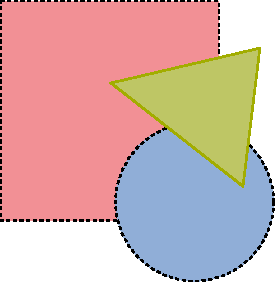
\includegraphics{shapes}

  \caption{Example Shapes from an SVG.}
  \label{fig:example_svg}
\end{figure}

\lipsum[42]



\subsection{Example Source Code}

\lipsum[1]

\begin{lstlisting}[
    language = C,
    caption  = {Example Source Code},
    label    = {list:example_src}
]
#include <stdio.h>

void quick_sort (int *a, int n) {
    int i, j, p, t;
    if (n < 2)
        return;
    p = a[n / 2];
    for (i = 0, j = n - 1;; i++, j--) {
        while (a[i] < p)
            i++;
        while (p < a[j])
            j--;
        if (i >= j)
            break;
        t = a[i];
        a[i] = a[j];
        a[j] = t;
    }
    quick_sort(a, i);
    quick_sort(a + i, n - i);
}

/* main routine */
int main (void) {
    int a[] = {4, 65, 2, -31, 0, 99, 2, 83, 782, 1};
    int n = sizeof a / sizeof a[0];
    int i;
    for (i = 0; i < n; i++)
        printf("%d%s", a[i], i == n - 1 ? "\n" : " ");
    quick_sort(a, n);
    for (i = 0; i < n; i++)
        printf("%d%s", a[i], i == n - 1 ? "\n" : " ");
    return 0;
}
\end{lstlisting}



\subsection{Example Subsection}

\lipsum[1]



\subsubsection{Example SubSubSection}

\lipsum[9]



\subsubsection{Example SubSubSection}

\lipsum[10]



\chapter{Conclusion \& Outlook}
\label{chap:conclusion}

\lipsum[1-4]



%-------------------------------------------------------------------------------
% Bibliography
%-------------------------------------------------------------------------------
%\backmatter
% unsrturl-custom works only with hyperref loaded
% use other styles like unsrt when hyperref is not loaded
\renewcommand\bibsection{\chapter*{Bibliography}\addcontentsline{toc}{chapter}{\protect Bibliography}}
%\bibliographystyle{unsrturl-custom}
\bibliographystyle{plainnat}
\bibliography{bibliography}



%-------------------------------------------------------------------------------
% Appendix
%-------------------------------------------------------------------------------
\appendix

\chapter{Uncertainty Estimation for Classification}
\section{Dirichlet Distribution Computations}

\subsection{Dirichlet distribution}

The Dirichlet distribution with concentration parameters $\bm \alpha = ( \alpha_1, \dots, \alpha_\nclass )$, where $\alpha_\iclass > 0$, has the probability density function:
\begin{equation}
    f(\bm x; \bm \alpha) =
    \frac{\prod_{\iclass=1}^\nclass \Gamma(\alpha_\iclass)}{\Gamma\left( \sum_{\iclass=1}^\nclass \alpha_\iclass \right)}
    \prod_{\iclass=1}^\nclass x_i^{\alpha_\iclass - 1}
\end{equation}
where $\Gamma$ is a gamma function:
\begin{align*}
    \Gamma(\alpha) = \int_0^\infty \alpha^{z-1} e^{-\alpha} dz
\end{align*}

\subsection{Closed-form formula for Bayesian loss.}

The novel Bayesian loss described in formula \ref{dirichlet_bayesian_loss} can be computed in closed form. For the sample $\vect{x}\dataix$, it is given by:
\begin{equation}
       \mathcal{L}\dataix = \underbrace{\E_{q(\mathbf{p}\dataix)}[\text{CE}(\mathbf{p}\dataix, \vect{y}\dataix)]}_{\text{(1)}} - \underbrace{H(q\dataix)}_{\text{(2)}}
\end{equation}

where the distribution $q$ belongs to the family of the Dirichlet distributions Dir$(\bm{\alpha}\dataix)$. The term (1) is the UCE loss \cite{uceloss}. Given that the observed class one-hot encoded by $\vect{y}\dataix$ is denoted by $\iclass*$, the term (1) is equal to:
\begin{equation}
\E_{q(\mathbf{p}\dataix)}[\text{CE}(\mathbf{p}\dataix, \vect{y}\dataix)] = \Psi(\alpha_{\iclass*}\dataix) - \Psi(\alpha_0\dataix)
\end{equation}
where $\Psi$ denotes the digamma function. The term (2) is the entropy of a Dirichlet distribution and is given by:
\begin{equation}
H(q\dataix) = \log B(\bm{\alpha}\dataix) + (\alpha_0\dataix - \nclass) \Psi(\alpha_0\dataix) - \sum_\iclass (\alpha_\iclass\dataix - 1) \Psi(\alpha_\iclass\dataix)
\end{equation}
where $B$ denotes the beta function.

\subsection{Epistemic covariance for in-distribution samples in \PostNetacro.}
\label{epistemic_variance_proof}

The epistemic distribution in \PostNetacro is a Dirichlet distribution Dir$(\bm{\alpha}\dataix)$ with the following concentration parameters $\alpha_\iclass\dataix = \beta_\iclass^\text{prior} + N \cdot \prob(\iclass | \latent\dataix; \phi) \cdot \prob(\latent\dataix; \phi)$ and $\alpha_0\dataix = \sum_\iclass \beta_\iclass^\text{prior} + N \cdot \prob(\latent\dataix; \phi)$. We can write the variance:
\begin{equation}
\begin{aligned}
\text{Var}_{\vect{p}\sim \Dir(\boldsymbol{\alpha}\dataix)}(p_\iclass) & = \frac{\alpha_\iclass (\alpha_0 - \alpha_\iclass)}{\alpha_0^2 (\alpha_0 + 1)}; \; \text{Cov}_{\vect{p}\sim \Dir(\boldsymbol{\alpha}\dataix)}(p_\iclass, p_{\iclass'}) & = \frac{-\alpha_\iclass\alpha_{\iclass'}}{\alpha_0^2 (\alpha_0 + 1)}
\end{aligned}
\end{equation}
For in-distribution data (i.e. $\prob(\latent\dataix; \phi) \rightarrow \infty$), we have $\text{Var}_{\vect{p}\sim \Dir(\boldsymbol{\alpha}\dataix)}(p_\iclass) = \mathcal{O}\left(\frac{\prob(\iclass | \latent\dataix; \phi)(1-\prob(\iclass | \latent\dataix; \phi))}{\prob(\latent\dataix; \phi) N}\right)$ and $\text{Cov}_{\vect{p}\sim \Dir(\boldsymbol{\alpha}\dataix)}(p_\iclass, p_{\iclass'}) = \mathcal{O}\left(\frac{-\prob(\iclass | \latent\dataix; \phi)\prob(\iclass' | \latent\dataix; \phi)}{\prob(\latent\dataix; \phi)N}\right)$. Hence both terms converge to $0$ when $\prob(\latent\dataix; \phi) \rightarrow \infty$.

\section{Model details}
\label{model_detais}

For vector datasets, all models share an architecture of 3 linear layers with Relu activation. A grid search in $[32, 64, 128]$ led to no significant changes in the performances. Therefore, we decided to use $64$ hidden units for each layer. For image datasets, we used LeakyRelu activation and add on the top 3 convolutional layers with kernel size of $5$, followed by a Max-pooling of size $2$. Alternatively, we used the VGG16 architecture with batch normalization \cite{vgg} adapted from PyTorch implementation \cite{pytorch}. All models are trained after a grid search for learning rate in $[1e^{-3}, 1e^{-5}]$. All models were optimized with Adam optimizer without further learning rate scheduling. We performed early stopping by checking loss improvement every $2$ epochs and a patience equal to $10$. We trained all models on GPUs (1TB SSD).

For the dropout models, we used $p_{\text{drop}} = .25$ after a grid search in $[.25, .5, .75]$ and sampled $10$ times for uncertainty estimation. As an indicator, the original paper \cite{dropout}, uses a dropout probability of $.5$ for MNIST. It also states that $10$ samples already lead to reasonable uncertainty estimates. For the ensemble models, we used $m=10$ networks after a grid search in $[2, 5, 10, 20]$. A greater number of networks was also found to give no great improvements in the original paper \cite{ensembles}. To be fair with these models, we distilled the knowledge of $10$ neural networks for Distribution Distillation. We also trained Prior Networks where target parameters $\beta_\text{in}=1e^2$ as suggested in original papers \cite{PriorNetworks, reverse-kl}.

For \PostNetacro, we used a 1D batch normalization after the encoder. Experiments on latent dimensions and density types are presented in following sections. If not explicitley mentioned otherwise, we used by default radial flow with a flow length of $6$ and a latent dimension of $6$. This leads to only $80$ parameters. Comparison with IAF are done with two layers of size $256$. In general, we found out that a latent dimension smaller or equal to the number of classes is sufficient. It enables classes to be orthogonal in the latent space if necessary.

All metrics have been scaled by $100$. We obtain numbers in $[0, 100]$  for all scores instead of $[0, 1]$.

\section{Datasets details}
\label{dataset_details}

For all datasets, we use 5 different random splits to train all models. We split the data in training, validation and test sets ($60\%$, $20\%$, $20\%$). In particular, we did not restrict to classic MNIST and CIFAR10 splits in order do prevent overfitting to a specific split.

We use one toy dataset composed of three 2D isotropic Gaussians corresponding to three classes. The Gaussians means are $[0, 2.]$, $[-1.73205081, -1.]$ and $[ 1.73205081, -1. ]$. The variance of the Gaussians is $0.2$. A visualization of the true distributions for the three Gaussians is given in Figure~\ref{visualization_gaussians}. The final dataset is composed in total of 1500 samples.

We use the segment vector dataset \cite{uci_datasets}, where the goal is to classify areas of images into $7$ classes (window, foliage, grass, brickface, path, cement, sky). We remove the class 'sky' from training and instead use it as the OOD dataset for OOD detection experiments. Each input is composed of $18$ attributes describing the image area. The dataset contains $2,310$ samples in total.

We further use the Sensorless Drive vector dataset \cite{uci_datasets}, where the goal is to classify extracted motor current measurements into $11$ different classes. We remove classes 10 and 11 from training and use them as the OOD dataset for OOD detection experiments. Each input is composed of $49$ attributes describing motor behaviour. The dataset contains $58,509$ samples in total.

Additionally, we use the MNIST image dataset \cite{mnist} where the goal is to classify pictures of hand-drawn digits into $10$ classes (from digit $0$ to digit $9$). Each input is composed of a $1 \times 28 \times 28$ tensor. The dataset contains $70,000$ samples. For OOD detection experiments, we use KMNIST \cite{kmnist} and FashionMNIST \cite{fashionmnist} containing images of Japanese characters and images of clothes, respectively. 

Finally, we use the CIFAR10 image dataset \cite{cifar10} where the goal is to classify a picture of objects into $10$ classes (airplane, automobile, bird, cat, deer, dog, frog, horse, ship, truck). Each input is a $3 \times 32 \times 32$ tensor. The dataset contains $60,000$ samples. For OOD detection experiments, we use street view house numbers (SVHN) \cite{svhn} containing images of numbers. For the dataset shift experiments, we use the classic split of CIFAR10 to avoid data leakage with the corrupted images from the test set that is provided online.

\section{Additional Experimental Results}
\label{sec:app_additional_results}

In this section, we present additional results for uncertainty estimation on other datasets. Tables \ref{fig:unc_segment_full}, \ref{fig:unc_sensorless_drive_full}, \ref{fig:unc_MNIST_full}, \ref{fig:ood_MNIST_full}, \ref{fig:unc_CIFAR10_full} show the performance of all models on the Segment, Sensorless Drive, MNIST, and CIFAR10 datasets. In the same way as for the other datasets, \PostNetacro is competitive for all metrics and show a significant improvement on calibration among Dirichlet parametrized models and on OOD detection tasks among all models. We evaluated the performances of all models on MNIST using different uncertainty measures and observed very correlated results (see Table~\ref{tab:MNIST++}). We compared different encoder architectures on CIFAR10 (see Fig.~\ref{tab:architecture_CIFAR10}). Without further parameter tuning, \PostNetacro adapted well to the convolutional architecture, AlexNet \cite{alexnet}, VGG \cite{vgg} and ResNet \cite{resnet}. For easier comparison, we also trained models on the classic CIFAR10 split (79\%, 5\%, 16\%) with VGG architecture. We noticed that a larger training set leads to better accuracy for all models.

We also show results of experiments with different latent dimensions (see Fig.~\ref{fig:latent_dim_segment}; \ref{fig:latent_dim_sensorless_drive}; \ref{fig:latent_dim_MNIST}; \ref{fig:latent_dim_CIFAR10}) and density types (MoG, radial, IAF) (see Tab.~\ref{fig:unc_segment_full}; \ref{fig:unc_sensorless_drive_full}; \ref{fig:unc_MNIST_full}; \ref{fig:ood_MNIST_full}; \ref{fig:unc_CIFAR10_full}) for all datasets. We remarked that \PostNetacro works with various type of densities even if using mixture of Gaussians presented more instability in practice. We observed no clear winner between Radial flow and IAF. We observed a bit lower performances for MoG which could be explained by its lack of expressiveness. Furthermore, we observed that a too high latent dimension would affect the performance.

Beside tables and figures with detailed metrics, we report additional visualizations. We present the uncertainty visualization on the input space for a 2D toy dataset (see Fig.~\ref{fig:visualization_grid}). We show this visualization for all models parametrizing Dirichlet distributions. \PostNetacro is the only model which is not overconfident for OOD data. In particular, it demonstrates the best fit of the true in-distribution data shown in figure \ref{visualization_gaussians}. Other models show overconfident prediction for OOD regions and fail even on this simple dataset. 

Furthermore, we plotted histograms of entropy of ID, OOD, OODom data for MNIST and CIFAR10 (see Fig~\ref{entropy_MNIST} and \ref{cifar_shifts}). For both datasets, \PostNetacro can easily distinguish between the three data types.

Finally, We also included the evolution of the uncertainty while interpolating linearly between images of MNIST (see Fig.~\ref{aleatoric_interpolation} and \ref{epistemic_interpolation}). It corresponds to a smooth walk in latent space. As shown in Figure \ref{aleatoric_interpolation}, \PostNetacro predicts correctly on clean images and outputs more balanced class predictions for mixed images. Additionally the Figure \ref{epistemic_interpolation} shows the evolution of the concentration parameters and consequently the epistemic uncertainty. We observe that the epistemic uncertainty (i.e. low $\alpha_\iclass$) is higher on mixed images which do not correspond to proper digits.

%%%%%%%%%%%%%%%%%%%%%%%%%%%%%%%%%%%%%%%%%%%%%%%%%%%
%%%%%%%%%%%%%%%%%%%%%%%%%%%%%%%%%%%%%%%%%%%%%%%%%%%
%\subsection{3-Gaussians Dataset}

\begin{figure}[ht]
    \centering
        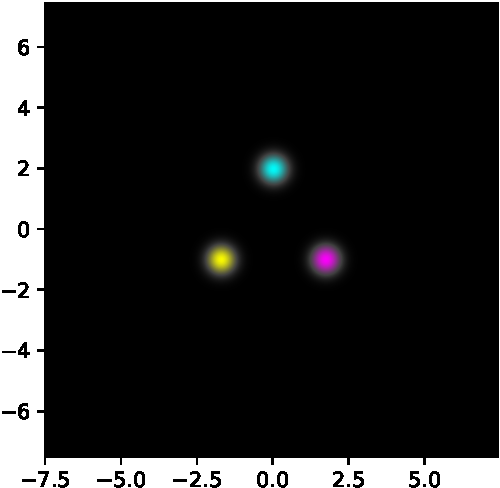
\includegraphics[width= 0.25 \columnwidth]{sections/006_neurips2020/figures/three_gaussians_dataset-crop.pdf}
        
    \caption{Three Gaussians toy dataset.}
    \label{visualization_gaussians}
\end{figure}

\begin{figure}[ht]
    \centering
        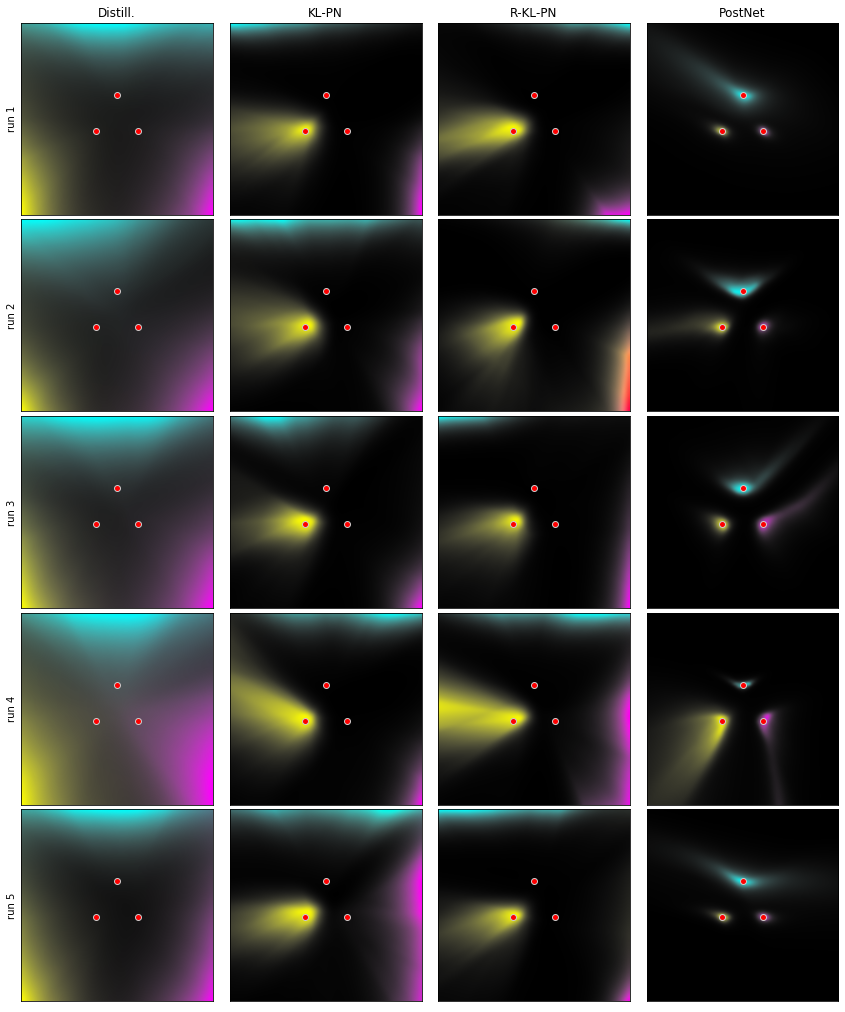
\includegraphics[width=1. \textwidth]{sections/006_neurips2020/figures/visualization-grid.png}
        
    \caption{Visualization of the concentration parameters predicted by Distribution Distillation, Prior Networks trained with KL and reverse KL divergence and \PostNet on a 3-Gaussians toy dataset over 5 runs. Red dots indicate the mean of the 3 Gaussians. Colours indicate class labels predicted by the models, dark regions correspond to high epistemic uncertainty. \PostNetacro consistently predicts low uncertainty around the training data and high uncertainty for OOD data.}
    \label{fig:visualization_grid}
\end{figure}

%%%%%%%%%%%%%%%%%%%%%%%%%%%%%%%%%%%%%%%%%%%%%%%%%%%
%%%%%%%%%%%%%%%%%%%%%%%%%%%%%%%%%%%%%%%%%%%%%%%%%%%
%\subsection{Segment Dataset}

\begin{table}[ht]
    \resizebox{1 \textwidth}{!}{%
\begin{tabular}{lllllll}
\toprule
{} &  \textbf{Acc.} & \textbf{Alea. Conf.} & \textbf{Epist. Conf.}  & \textbf{Brier} & \textbf{OOD Alea.} & \textbf{OOD Epist.} \\
\midrule
\midrule
\textbf{Drop Out       } &  95.25$\pm$0.1 &        99.75$\pm$0.0 &          99.43$\pm$0.0 &  11.89$\pm$0.2 &      41.48$\pm$0.5 &       43.11$\pm$0.6 \\
\textbf{Ensemble       } &  *97.27$\pm$0.1 &        *99.88$\pm$0.0 &          *99.85$\pm$0.0 &   *7.64$\pm$0.2 &      54.76$\pm$1.6 &       58.13$\pm$1.7 \\
\midrule
\textbf{Distill.       } &  96.21$\pm$0.1 &        99.82$\pm$0.0 &           \textbf{99.8$\pm$0.0} &  57.77$\pm$0.6 &      37.12$\pm$0.5 &       35.83$\pm$0.4 \\
\textbf{KL-PN          } &  95.61$\pm$0.1 &        99.79$\pm$0.0 &          99.76$\pm$0.0 &  16.84$\pm$0.3 &      65.62$\pm$2.4 &       57.07$\pm$3.7 \\
\textbf{RKL-PN         } &  96.36$\pm$0.2 &        99.71$\pm$0.0 &          99.58$\pm$0.0 &  11.97$\pm$0.1 &      75.46$\pm$2.4 &       51.02$\pm$0.6 \\
\textbf{PostN Rad. (2) } &  95.76$\pm$0.1 &        99.23$\pm$0.1 &          98.82$\pm$0.1 &  13.33$\pm$1.3 &      92.75$\pm$1.3 &       90.41$\pm$1.5 \\
\textbf{PostN Rad. (6) } &  96.52$\pm$0.2 &        99.82$\pm$0.0 &          99.43$\pm$0.0 &   8.69$\pm$0.3 &      98.27$\pm$0.2 &       98.09$\pm$0.3 \\
\textbf{PostN Rad. (10)} &   94.9$\pm$0.2 &        99.51$\pm$0.0 &          98.57$\pm$0.1 &  12.22$\pm$0.7 &      95.53$\pm$0.8 &       97.51$\pm$0.7 \\
\textbf{PostN IAF (2)  } &  93.94$\pm$0.3 &        99.02$\pm$0.1 &           98.3$\pm$0.2 &  15.33$\pm$0.7 &       \textbf{*98.3$\pm$0.3} &       \textbf{*99.33$\pm$0.1} \\
\textbf{PostN IAF (6)  } &  95.71$\pm$0.2 &        99.63$\pm$0.0 &          99.11$\pm$0.1 &  10.16$\pm$0.3 &      96.92$\pm$0.9 &       98.17$\pm$0.6 \\
\textbf{PostN IAF (10) } &  \textbf{96.92$\pm$0.1} &        \textbf{99.83$\pm$0.0} &          99.49$\pm$0.0 &   \textbf{8.45$\pm$0.4} &      95.75$\pm$1.1 &       96.74$\pm$0.9 \\
\textbf{PostN MoG (2)  } &  63.43$\pm$5.3 &        79.61$\pm$6.2 &          79.05$\pm$6.1 &  54.14$\pm$5.4 &      90.87$\pm$1.4 &       91.62$\pm$1.4 \\
\textbf{PostN MoG (6)  } &  89.75$\pm$2.5 &        95.28$\pm$1.6 &          93.15$\pm$2.1 &  24.42$\pm$4.3 &      96.04$\pm$1.3 &       97.71$\pm$0.8 \\
\textbf{PostN MoG (10) } &  94.44$\pm$0.5 &        99.64$\pm$0.1 &          99.08$\pm$0.2 &  14.79$\pm$1.3 &      91.14$\pm$1.5 &       90.82$\pm$1.3 \\
\bottomrule
\end{tabular}

    }
    \caption{Results on Segment dataset with all models. It shows results with different density types. Number into parentheses indicates flow size (for radial flow and IAF) or number of components (for MoG). Bold numbers indicate best score among Dirichlet parametrized models and starred numbers indicate best scores among all models.}
    \label{fig:unc_segment_full}
\end{table}

\begin{table}[ht]
    \resizebox{1 \textwidth}{!}{%
\begin{tabular}{lllllll}
\toprule
{} &  \textbf{Acc.} & \textbf{Alea. Conf.} & \textbf{Epist. Conf.} & \textbf{Brier} & \textbf{OOD Alea.} & \textbf{OOD Epist.} \\
\midrule
\midrule
\textbf{PostN: No-Flow      } & \cellcolor{Gray} 93.13$\pm$0.3 &        99.48$\pm$0.1 & 98.41$\pm$0.3 & \cellcolor{Gray} 12.94$\pm$0.3 & \cellcolor{Gray}  47.3$\pm$2.9 & \cellcolor{Gray} 35.49$\pm$0.3 \\
\textbf{PostN: No-Bayes-Loss} & \cellcolor{Gray} 93.94$\pm$0.8 &  98.53$\pm$0.3 & \cellcolor{Gray}  96.08$\pm$1.1 & \cellcolor{Gray} 16.15$\pm$1.9 & \cellcolor{Gray} 94.71$\pm$1.0 & \cellcolor{Gray} 95.92$\pm$0.8 \\
\textbf{PostN: Seq-No-Bn    } & \cellcolor{Gray} 18.94$\pm$1.1 & \cellcolor{Gray}  20.42$\pm$1.7 & \cellcolor{Gray}  20.42$\pm$1.7 & \cellcolor{Gray} 91.29$\pm$0.0 & \cellcolor{Gray} 58.91$\pm$0.8 & \cellcolor{Gray} 58.43$\pm$0.8 \\
\textbf{PostN: Seq-Bn       } & \cellcolor{Gray} 93.89$\pm$0.1 &        99.38$\pm$0.1 &  98.93$\pm$0.0 & \cellcolor{Gray} 14.64$\pm$0.3 &      98.02$\pm$0.4 &       99.93$\pm$0.0 \\
\bottomrule
\end{tabular}

    }
    \caption{Ablation study results on Segment dataset. Gray cells indicate significant drops in scores compare to the complete \PostNetacro Rad. (6) model in Table \ref{fig:unc_segment_full}.}
    \label{fig:ablation_segment}
\end{table}

\begin{figure}[ht]
    \centering
    \begin{subfigure}[t]{0.33 \textwidth}
        \centering
        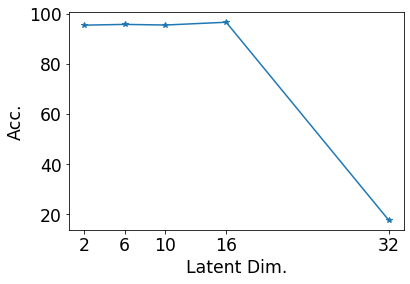
\includegraphics[width=1. \textwidth]{sections/006_neurips2020/figures/lat_dim_seg_acc.png}
    \end{subfigure}%   
    \begin{subfigure}[t]{0.33 \textwidth}
        \centering
        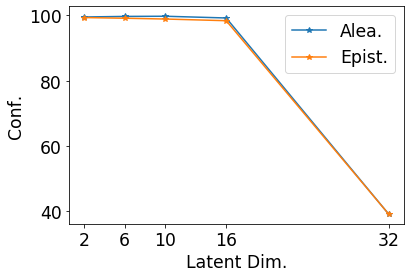
\includegraphics[width=1. \textwidth]{sections/006_neurips2020/figures/lat_dim_seg_conf.png}
    \end{subfigure}% 
    
    \begin{subfigure}[t]{0.33 \textwidth}
        \centering
        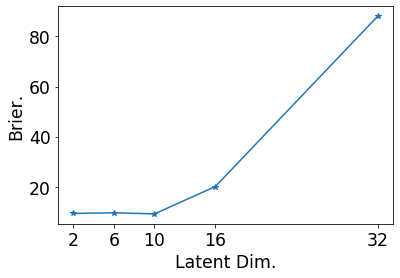
\includegraphics[width=1. \textwidth]{sections/006_neurips2020/figures/lat_dim_seg_brier.png}
    \end{subfigure}%
    \begin{subfigure}[t]{0.33 \textwidth}
        \centering
        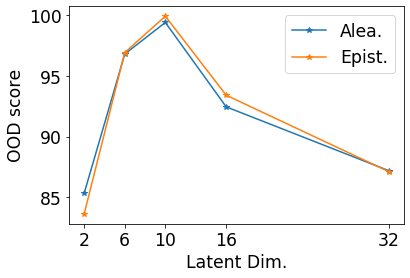
\includegraphics[width=1. \textwidth]{sections/006_neurips2020/figures/lat_dim_seg_ood.png}
    \end{subfigure}%

    \caption{Accuracy and uncertainty scores of \PostNetacro with latent dimension in $[2, 6, 10, 32]$ on the Segment dataset. We observed that the performances remains high for small dimensions (i.e. $2$, $6$, $10$) and drop for a too high dimension (i.e. $32$).}
    \label{fig:latent_dim_segment}
\end{figure}

%%%%%%%%%%%%%%%%%%%%%%%%%%%%%%%%%%%%%%%%%%%%%%%%%%%
%%%%%%%%%%%%%%%%%%%%%%%%%%%%%%%%%%%%%%%%%%%%%%%%%%%
%\subsection{Sensorless Drive Dataset}

\begin{table}[ht]
    \resizebox{1 \textwidth}{!}{%
\begin{tabular}{lllllll}
\toprule
{} &  \textbf{Acc.} & \textbf{Alea. Conf.} & \textbf{Epist. Conf.} & \textbf{Brier} & \textbf{OOD Alea.} & \textbf{OOD Epist.} \\
\midrule
\midrule
\textbf{Drop Out       } &  89.32$\pm$0.2 &        98.21$\pm$0.1 &         95.24$\pm$0.2 &  28.86$\pm$0.4 &      35.41$\pm$0.4 &       40.61$\pm$0.7 \\
\textbf{Ensemble       } &  99.37$\pm$0.0 &        99.99$\pm$0.0 &         *99.98$\pm$0.0 &   2.47$\pm$0.1 &      50.01$\pm$0.0 &       50.62$\pm$0.1 \\
\midrule
\textbf{Distill.       } &  93.66$\pm$1.5 &        98.29$\pm$0.5 &         98.15$\pm$0.5 &  44.94$\pm$1.4 &       32.1$\pm$0.6 &       31.17$\pm$0.2 \\
\textbf{KL-PN          } &  94.77$\pm$0.9 &        99.52$\pm$0.1 &         99.47$\pm$0.1 &  21.47$\pm$1.9 &      35.48$\pm$0.8 &        33.2$\pm$0.6 \\
\textbf{RKL-PN         } &  99.42$\pm$0.0 &        99.96$\pm$0.0 &         99.89$\pm$0.0 &   9.07$\pm$0.1 &      45.89$\pm$1.6 &       38.14$\pm$0.8 \\
\textbf{PostN Rad. (2) } &  96.07$\pm$0.0 &        99.28$\pm$0.0 &         98.88$\pm$0.0 &  19.94$\pm$0.0 &      \textbf{*98.22$\pm$0.0} &       \textbf{*98.03$\pm$0.0} \\
\textbf{PostN Rad. (6) } &  98.02$\pm$0.1 &        99.89$\pm$0.0 &         99.47$\pm$0.0 &   5.51$\pm$0.2 &      72.89$\pm$0.8 &       88.73$\pm$0.5 \\
\textbf{PostN Rad. (10)} &   97.3$\pm$0.0 &        99.82$\pm$0.0 &         99.31$\pm$0.0 &   7.93$\pm$0.0 &      66.65$\pm$0.0 &       87.91$\pm$0.0 \\
\textbf{PostN IAF (2)  } &  99.19$\pm$0.0 &        99.98$\pm$0.0 &         99.78$\pm$0.0 &   2.45$\pm$0.0 &      78.13$\pm$0.0 &        85.9$\pm$0.0 \\
\textbf{PostN IAF (6)  } &  99.11$\pm$0.1 &        99.98$\pm$0.0 &         99.72$\pm$0.0 &   2.71$\pm$0.1 &      78.48$\pm$0.7 &       86.47$\pm$0.5 \\
\textbf{PostN IAF (10) } &  \textbf{*99.52$\pm$0.0} &        \textbf{*100.0$\pm$0.0} &         \textbf{99.92$\pm$0.0}&   \textbf{*1.43$\pm$0.1} &      82.96$\pm$0.8 &       88.65$\pm$0.4 \\
\textbf{PostN MoG (2)  } &  59.63$\pm$4.8 &         72.2$\pm$4.7 &         70.38$\pm$4.8 &  68.41$\pm$4.6 &       67.2$\pm$3.1 &        72.3$\pm$2.9 \\
\textbf{PostN MoG (6)  } &  96.83$\pm$0.2 &        99.72$\pm$0.0 &         99.16$\pm$0.1 &  13.24$\pm$1.0 &      59.82$\pm$2.3 &       60.61$\pm$2.6 \\
\textbf{PostN MoG (10) } &  96.65$\pm$0.2 &        99.64$\pm$0.0 &         99.12$\pm$0.1 &  13.12$\pm$1.1 &      61.54$\pm$1.8 &       65.35$\pm$2.0 \\
\bottomrule
\end{tabular}

    }
    \caption{Results on Sensorless Drive dataset with all models. It shows results with different density types. Number into parentheses indicates flow size (for radial flow and IAF) or number of components (for MoG).}
    \label{fig:unc_sensorless_drive_full}
\end{table}

\begin{figure}[ht]
    \centering
    \begin{subfigure}[t]{0.33 \textwidth}
        \centering
        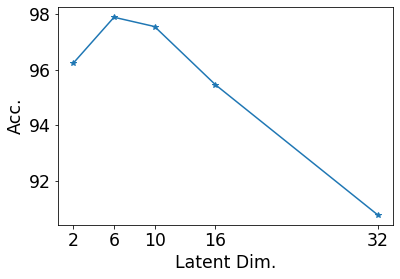
\includegraphics[width=1. \textwidth]{sections/006_neurips2020/figures/lat_dim_sen_acc.png}
    \end{subfigure}%   
    \begin{subfigure}[t]{0.33 \textwidth}
        \centering
        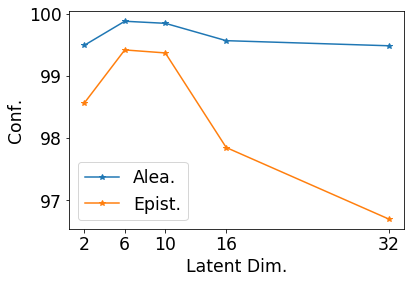
\includegraphics[width=1. \textwidth]{sections/006_neurips2020/figures/lat_dim_sen_conf.png}
    \end{subfigure}% 
    
    \begin{subfigure}[t]{0.33 \textwidth}
        \centering
        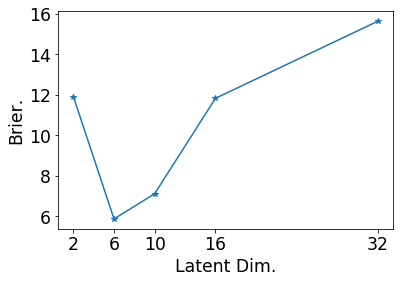
\includegraphics[width=1. \textwidth]{sections/006_neurips2020/figures/lat_dim_sen_brier.png}
    \end{subfigure}%
    \begin{subfigure}[t]{0.33 \textwidth}
        \centering
        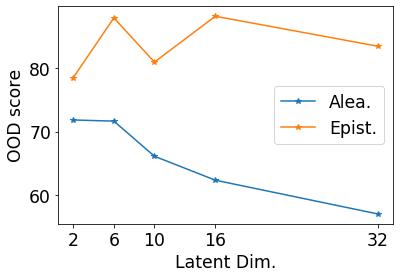
\includegraphics[width=1. \textwidth]{sections/006_neurips2020/figures/lat_dim_sen_ood.png}
    \end{subfigure}%

    \caption{Accuracy and uncertainty scores of \PostNetacro with latent dimension in $[2, 6, 10, 32]$ on the Sensorless Drive dataset. OOD scores are computed against the left out sky class. We observed that the performances remains high for medium dimensions (i.e. $6$, $10$) and drop for a too high dimension (i.e. $32$).}
    \label{fig:latent_dim_sensorless_drive}
\end{figure}

%%%%%%%%%%%%%%%%%%%%%%%%%%%%%%%%%%%%%%%%%%%%%%%%%%%
%%%%%%%%%%%%%%%%%%%%%%%%%%%%%%%%%%%%%%%%%%%%%%%%%%%
%\subsection{MNIST Dataset}

\begin{figure}[t!]
    \centering
    \begin{subfigure}[t]{0.46 \columnwidth}
        \centering
        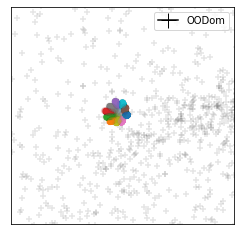
\includegraphics[width=0.5 \textwidth]{sections/006_neurips2020/figures/2D_latent_klpn_3.png}
         \caption{ID/OOD data (PriorNetworks)}
    \end{subfigure}%
    \begin{subfigure}[t]{0.46 \columnwidth}
        \centering
        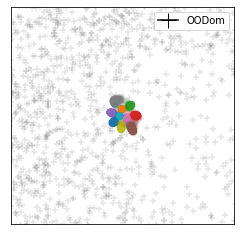
\includegraphics[width=0.5 \textwidth]{sections/006_neurips2020/figures/2D_latent_ours_bn_3.png}
         \caption{ID/OOD data (\PostNetacro)}
    \end{subfigure}%
    \caption{This figure should be seen in perspective with Fig.~\ref{fig:mnist_2D_latent_space}. We plot FashionMNIST OODom data with black crosses to show where these data would land. OODom data were not used for training the models, A comparison of Fig.~\ref{fig:mnist_2D_latent_space_2}(a) with Fig.~\ref{fig:mnist_2D_latent_space}(b) show that Prior Network assigns high certainty to OODom data. In contrast, a comparison of Fig.~\ref{fig:mnist_2D_latent_space_2}(b) and Fig.~\ref{fig:mnist_2D_latent_space}(c) shows that \PostNet assigns low uncertainty to OODom data as desired.}
    \label{fig:mnist_2D_latent_space_2}
\end{figure}

\begin{figure}[ht]
    \centering
    \begin{subfigure}[t]{.5 \columnwidth}
        \centering
        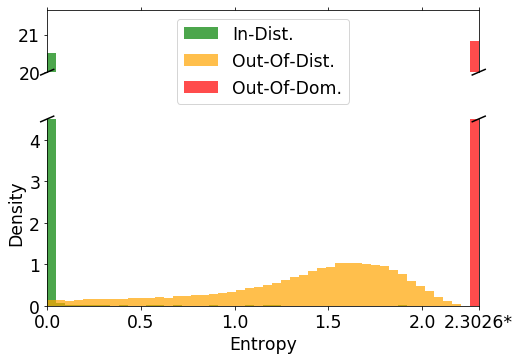
\includegraphics[width=1 \textwidth]{sections/006_neurips2020/figures/entropy_MNIST.png}
        \caption{MNIST}    
        \end{subfigure}%   
    \caption{Histograms of the entropy of the predicted categorical distributions for in-distribution (green), out-of-distribution (yellow) and out-of-domain (red) data. The value $2.3026^*$ denotes the maximal entropy achievable for a categorical distribution with 10 classes. We use MNIST, FashionMNIST and the unscaled version of FashionMNIST as in-distribution, out-of-distribution and out-of-domain data. \PostNetacro clearly distinguishes between the three types of data with low entropy for in-distribution data and high entropy for out-of-distribution, and close to the maximum possible entropy for out-of-domain data.}
    \label{entropy_MNIST}
\end{figure}

\begin{figure}[ht]
    \centering
        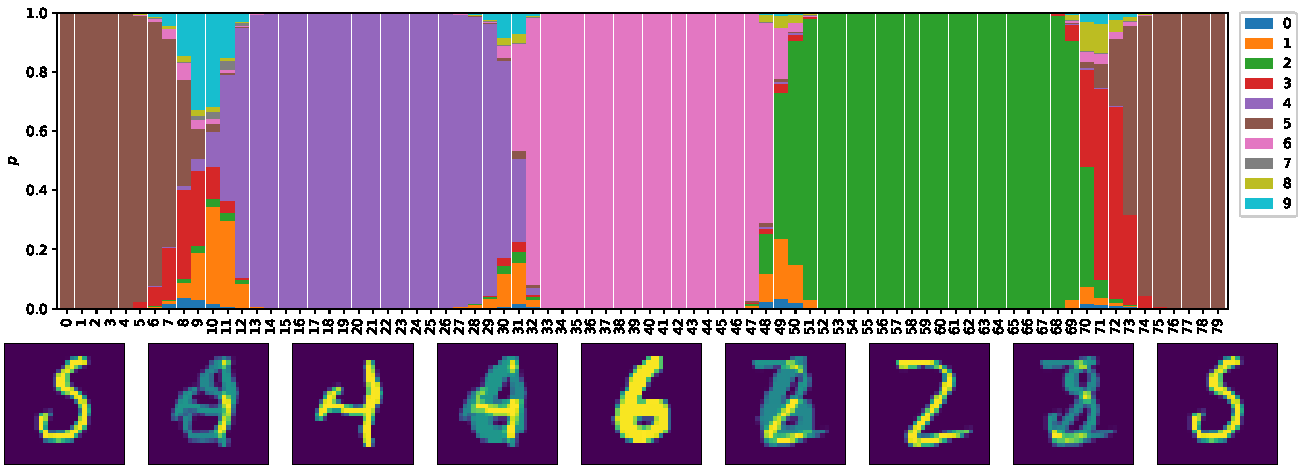
\includegraphics[width=.9 \textwidth]{sections/006_neurips2020/figures/image_interpolation_uncertainty3.pdf}
        
    \caption{Evolution of the probability predictions when interpolating linearly between four MNIST images. The interpolation goes from the clean digits $5$, $4$, $6$ and $2$ in a cyclic way with $20$ interpolated images between each pair. As desired, We can observe correct predictions around clean images with higher (aleatoric) uncertainty for mixed images, and smooth transitions in between.}
    \label{aleatoric_interpolation}
\end{figure}

\begin{figure}[ht]
    \centering
        \includegraphics[width=.9 \textwidth]{sections/006_neurips2020/figures/image_interpolation_uncertainty4.pdf}
        
    \caption{Evolution of the concentration parameters predictions when interpolating linearly between four MNIST images. The interpolation goes from the clean digits $5$, $4$, $6$ and $2$ in a cyclic way with $20$ interpolated images between each pair. As desired, we can observe correct and confident predictions around clean images with higher (epistemic) uncertainty for mixed images.}
    \label{epistemic_interpolation}
\end{figure}

\begin{table}[ht]
\centering
   % \resizebox{1 \textwidth}{!}{%
\begin{tabular}{lllll}
\toprule
{} &   \textbf{Acc.} & \textbf{Alea. Conf.} & \textbf{Epist. Conf.}  &  \textbf{Brier} \\
\midrule
\midrule
\textbf{Drop Out       } &  99.26$\pm$0.0 &       99.98$\pm$0.0 &         99.97$\pm$0.0 &   1.78$\pm$0.0 \\
\textbf{Ensemble       } &  *99.35$\pm$0.0 &       *99.99$\pm$0.0 &         *99.98$\pm$0.0 &   1.67$\pm$0.0 \\
\midrule
\textbf{Distill.       } &  \textbf{99.34$\pm$0.}0 &       \textbf{99.98$\pm$0.0} &         \textbf{*99.98$\pm$0.}0 &  72.55$\pm$0.2 \\
\textbf{KL-PN          } &  99.01$\pm$0.0 &       99.92$\pm$0.0 &         99.95$\pm$0.0 &  10.82$\pm$0.0 \\
\textbf{RKL-PN         } &  99.21$\pm$0.0 &       99.67$\pm$0.0 &         99.57$\pm$0.0 &   9.76$\pm$0.0 \\
\textbf{RKL-PN w/ F.   } &   99.2$\pm$0.0 &       99.75$\pm$0.0 &         99.68$\pm$0.0 &    9.9$\pm$0.0 \\
\textbf{PostN Rad. (2) } &  \textbf{99.34$\pm$0.0} &       \textbf{99.98$\pm$0.0} &         99.97$\pm$0.0 &   \textbf{*1.25$\pm$0.0} \\
\textbf{PostN Rad. (6) } &  99.28$\pm$0.0 &       99.97$\pm$0.0 &         99.96$\pm$0.0 &   1.36$\pm$0.0 \\
\textbf{PostN Rad. (10)} &  99.22$\pm$0.0 &       99.97$\pm$0.0 &         99.97$\pm$0.0 &   1.41$\pm$0.0 \\
\textbf{PostN IAF (2)  } &  99.06$\pm$0.0 &       99.96$\pm$0.0 &         99.94$\pm$0.0 &   1.48$\pm$0.0 \\
\textbf{PostN IAF (6)  } &  99.08$\pm$0.0 &       99.96$\pm$0.0 &         99.94$\pm$0.0 &   1.45$\pm$0.1 \\
\textbf{PostN IAF (10) } &  98.97$\pm$0.0 &       99.96$\pm$0.0 &         99.94$\pm$0.0 &   1.61$\pm$0.0 \\
\textbf{PostN MoG (2)  } &  76.41$\pm$2.3 &       99.93$\pm$0.0 &         99.92$\pm$0.0 &  23.23$\pm$2.2 \\
\textbf{PostN MoG (6)  } &  99.21$\pm$0.0 &       99.94$\pm$0.0 &         99.92$\pm$0.0 &   1.61$\pm$0.0 \\
\textbf{PostN MoG (10) } &  99.22$\pm$0.0 &       99.94$\pm$0.0 &         99.92$\pm$0.0 &   1.53$\pm$0.0 \\
\bottomrule
\end{tabular}
  %  }
    \caption{Accuracy, confidence and calibration results on MNIST dataset with all models. It shows results with different density types. Number into parentheses indicates flow size (for radial flow and IAF) or number of components (for MoG). Bold numbers indicate best score among Dirichlet parametrized models and starred numbers indicate best scores among all models.}
    \label{fig:unc_MNIST_full}
\end{table}

\begin{table}[ht]
    \resizebox{1 \textwidth}{!}{%
\begin{tabular}{lllllllll}
\toprule
{} & \textbf{OOD K.} & \textbf{OOD K.} & \textbf{OOD F.} & \textbf{OOD F.} & \textbf{OODom K.} & \textbf{OODom K.} & \textbf{OODom F.} & \textbf{OODom F.} \\
{} & \textbf{Alea.} & \textbf{Epist.} & \textbf{Alea.} & \textbf{Epist.} & \textbf{Alea.} & \textbf{Epist.} & \textbf{Alea.} & \textbf{Epist.} \\
\midrule
\midrule
\textbf{Drop Out       } &          94.0$\pm$0.1 &          93.01$\pm$0.2 &         96.56$\pm$0.2 &           95.0$\pm$0.2 &           31.59$\pm$0.5 &            31.97$\pm$0.5 &            27.2$\pm$1.1 &            27.52$\pm$1.1 \\
\textbf{Ensemble       } &         *97.12$\pm$0.0 &           *96.5$\pm$0.0 &         98.15$\pm$0.1 &          96.76$\pm$0.0 &            41.7$\pm$0.3 &            42.25$\pm$0.3 &           37.22$\pm$1.0 &            37.73$\pm$1.0 \\
\midrule
\textbf{Distill.       } &         \textbf{96.64$\pm$0.1} &          85.17$\pm$1.0 &         98.83$\pm$0.0 &          94.09$\pm$0.4 &           11.49$\pm$0.3 &            10.66$\pm$0.2 &           13.82$\pm$0.5 &            12.03$\pm$0.3 \\
\textbf{KL-PN          } &         92.97$\pm$1.2 &          93.39$\pm$1.0 &         98.44$\pm$0.1 &          98.16$\pm$0.0 &            9.54$\pm$0.1 &             9.78$\pm$0.1 &            9.57$\pm$0.1 &            10.06$\pm$0.1 \\
\textbf{RKL-PN         } &         60.76$\pm$2.9 &          53.76$\pm$3.4 &         78.45$\pm$3.1 &          72.18$\pm$3.6 &            9.35$\pm$0.1 &             8.94$\pm$0.0 &            9.53$\pm$0.1 &             8.96$\pm$0.0 \\
\textbf{RKL-PN w/ F.   } &         81.34$\pm$4.5 &          78.07$\pm$4.8 &         \textbf{*100.0$\pm$0.0} &          \textbf{*100.0$\pm$0.0} &            9.24$\pm$0.1 &             9.08$\pm$0.1 &           88.96$\pm$4.4 &            87.49$\pm$5.0 \\
\textbf{PostN Rad. (2) } &         95.49$\pm$0.3 &          93.12$\pm$0.7 &          96.2$\pm$0.3 &           94.6$\pm$0.4 &           \textbf{*100.0$\pm$0.0} &            \textbf{*100.0$\pm$0.0} &           \textbf{*100.0$\pm$0.0} &            \textbf{*100.0$\pm$0.0} \\
\textbf{PostN Rad. (6) } &         95.75$\pm$0.2 &          \textbf{94.59$\pm$0.3} &         97.78$\pm$0.2 &          97.24$\pm$0.3 &           \textbf{*100.0$\pm$0.0} &            \textbf{*100.0$\pm$0.0} &           \textbf{*100.0$\pm$0.0} &            \textbf{*100.0$\pm$0.0} \\
\textbf{PostN Rad. (10)} &         95.46$\pm$0.4 &          94.19$\pm$0.4 &         97.33$\pm$0.2 &          96.75$\pm$0.3 &           \textbf{*100.0$\pm$0.0} &            \textbf{*100.0$\pm$0.0} &           \textbf{*100.0$\pm$0.0} &            \textbf{*100.0$\pm$0.0} \\
\textbf{PostN IAF (2)  } &         92.24$\pm$0.3 &          91.75$\pm$0.3 &         96.58$\pm$0.2 &           96.6$\pm$0.2 &           \textbf{*100.0$\pm$0.0} &            \textbf{*100.0$\pm$0.0} &           \textbf{*100.0$\pm$0.0} &            \textbf{*100.0$\pm$0.0} \\
\textbf{PostN IAF (6)  } &         90.74$\pm$0.6 &          90.63$\pm$0.6 &         93.66$\pm$0.5 &          93.17$\pm$0.6 &           \textbf{*100.0$\pm$0.0} &            \textbf{*100.0$\pm$0.0} &           \textbf{*100.0$\pm$0.0} &            \textbf{*100.0$\pm$0.0} \\
\textbf{PostN IAF (10) } &         87.08$\pm$0.2 &          86.52$\pm$0.3 &         92.34$\pm$0.6 &          91.27$\pm$0.9 &           \textbf{*100.0$\pm$0.0} &            \textbf{*100.0$\pm$0.0} &           \textbf{*100.0$\pm$0.0} &            \textbf{*100.0$\pm$0.0} \\
\textbf{PostN MoG (2)  } &         74.27$\pm$2.0 &          73.34$\pm$1.9 &         76.99$\pm$2.0 &          76.74$\pm$1.9 &           \textbf{*100.0$\pm$0.0} &            \textbf{*100.0$\pm$0.0} &           99.99$\pm$0.0 &            99.99$\pm$0.0 \\
\textbf{PostN MoG (6)  } &         84.67$\pm$1.5 &          81.46$\pm$1.9 &         88.98$\pm$1.7 &          87.07$\pm$2.1 &           \textbf{*100.0$\pm$0.0} &            \textbf{*100.0$\pm$0.0} &           \textbf{*100.0$\pm$0.0} &            \textbf{*100.0$\pm$0.0} \\
\textbf{PostN MoG (10) } &         85.14$\pm$1.3 &          81.12$\pm$1.5 &         94.43$\pm$0.8 &           93.8$\pm$1.0 &           \textbf{*100.0$\pm$0.0} &            \textbf{*100.0$\pm$0.0} &           \textbf{*100.0$\pm$0.0} &            \textbf{*100.0$\pm$0.0} \\
\bottomrule
\end{tabular}

    }
    \caption{OOD results on MNIST dataset with all models. It shows results with different density types. Number into parentheses indicates flow size (for radial flow and IAF) or number of components (for MoG).}
    \label{fig:ood_MNIST_full}
\end{table}

\begin{table}[ht]
\centering
    \resizebox{1. \textwidth}{!}{%
\begin{tabular}{lllllllll}
\toprule
{} & \textbf{OOD K. $\alpha_0$/var.} & \textbf{OOD K. MI.} & \textbf{OOD F. $\alpha_0$/var.} & \textbf{OOD F. MI.} & \textbf{OODom K. $\alpha_0$/var.} & \textbf{OODom K. MI.} & \textbf{OODom F. $\alpha_0$/var.} & \textbf{OODom F. MI} \\
\midrule
\midrule
\textbf{Ensemble     } &          *97.19$\pm$0.0 &       *97.44$\pm$0.0 &          97.53$\pm$0.1 &       97.69$\pm$0.1 &            42.36$\pm$0.3 &         42.38$\pm$0.3 &            37.85$\pm$1.1 &        37.86$\pm$1.1 \\
\midrule
\textbf{RKL-PN       } &          54.11$\pm$3.4 &        54.9$\pm$3.3 &          72.54$\pm$3.6 &       73.33$\pm$3.5 &             8.94$\pm$0.0 &          8.94$\pm$0.0 &             8.96$\pm$0.0 &         8.96$\pm$0.0 \\
\textbf{RKL-PN  w/ F.} &           78.4$\pm$4.8 &       78.73$\pm$4.8 &          \textbf{*100.0$\pm$0.0} &       \textbf{*100.0$\pm$0.0} &             9.08$\pm$0.1 &          9.08$\pm$0.1 &             87.49$\pm$5.0 &        87.49$\pm$5.0 \\
\textbf{PostN        } &          \textbf{96.04$\pm$0.2} &       \textbf{96.05$\pm$0.2} &          98.17$\pm$0.2 &       98.17$\pm$0.2 &            \textbf{*100.0$\pm$0.0} &         \textbf{*100.0$\pm$0.0} &            \textbf{*100.0$\pm$0.0} &        \textbf{*100.0$\pm$0.0} \\
\bottomrule
\end{tabular}

    }
    \vspace{-0.2cm}
    \caption{\footnotesize{OOD detection on MNIST with other uncertainty measures. Mutual Information \cite{PriorNetworks} and $\alpha_0$ (Dirichlet) / variance (Ensemble) results are highly correlated.}}
    \label{tab:MNIST++}
    \vspace{-.0cm}
\end{table}

\begin{figure}[ht]
    \centering
    \begin{subfigure}[t]{0.33 \textwidth}
        \centering
        \includegraphics[width=1. \textwidth]{sections/006_neurips2020/figures/lat_dim_minst_acc.png}
    \end{subfigure}%   
    \begin{subfigure}[t]{0.33 \textwidth}
        \centering
        \includegraphics[width=1. \textwidth]{sections/006_neurips2020/figures/lat_dim_minst_conf.png}
    \end{subfigure}%   
    \begin{subfigure}[t]{0.33 \textwidth}
        \centering
        \includegraphics[width=1. \textwidth]{sections/006_neurips2020/figures/lat_dim_minst_brier.png}
    \end{subfigure}%

    \begin{subfigure}[t]{0.33 \textwidth}
        \centering
        \includegraphics[width=1. \textwidth]{sections/006_neurips2020/figures/lat_dim_minst_ood_1.png}
    \end{subfigure}%   
    \begin{subfigure}[t]{0.33 \textwidth}
        \centering
        \includegraphics[width=1. \textwidth]{sections/006_neurips2020/figures/lat_dim_minst_ood_2.png}
    \end{subfigure}%
    
    \begin{subfigure}[t]{0.33 \textwidth}
        \centering
        \includegraphics[width=1. \textwidth]{sections/006_neurips2020/figures/lat_dim_minst_ood_3.png}
    \end{subfigure}%
    \begin{subfigure}[t]{0.33 \textwidth}
        \centering
        \includegraphics[width=1. \textwidth]{sections/006_neurips2020/figures/lat_dim_minst_ood_4.png}
    \end{subfigure}%

    \caption{Accuracy and uncertainty scores of \PostNetacro with latent dimension in $[2, 6, 10, 32]$ on the MNIST dataset. OOD and OODom scores are computed against scaled and unscaled KMNIST and FashionMNIST datasets. We observed that the performances remains high for medium dimensions (i.e. $6$, $10$) and drop for a too high dimension (i.e. $32$).}
    \label{fig:latent_dim_MNIST}
\end{figure}

%%%%%%%%%%%%%%%%%%%%%%%%%%%%%%%%%%%%%%%%%%%%%%%%%%%
%%%%%%%%%%%%%%%%%%%%%%%%%%%%%%%%%%%%%%%%%%%%%%%%%%%
%\subsection{CIFAR10 Dataset}

\begin{table}[ht]
    \resizebox{1 \textwidth}{!}{%
\begin{tabular}{lllllllll}
\toprule
{} &  \textbf{Acc.} & \textbf{Alea. Conf.} & \textbf{Epist. Conf.}  & \textbf{Brier} & \textbf{OOD Alea.} & \textbf{OOD Epist.} & \textbf{OODom Alea.} & \textbf{OODom Epist.} \\
\midrule
\midrule
\textbf{Drop Out       } &  71.73$\pm$0.2 &        92.18$\pm$0.1 &          84.38$\pm$0.3 &  49.76$\pm$0.2 &      72.94$\pm$0.3 &       41.68$\pm$0.5 &         28.3$\pm$1.8 &          47.1$\pm$3.3 \\
\textbf{Ensemble       } &  *81.24$\pm$0.1 &        *96.61$\pm$0.0 &          93.25$\pm$0.1 &  38.88$\pm$0.1 &      *77.82$\pm$0.2 &       55.17$\pm$0.3 &        63.18$\pm$1.1 &         89.97$\pm$0.9 \\
\midrule
\textbf{Distill.       } &  72.11$\pm$0.4 &        91.72$\pm$0.2 &          90.73$\pm$0.2 &  88.04$\pm$0.1 &      \textbf{75.63$\pm$0.6} &       52.18$\pm$2.1 &        17.76$\pm$0.0 &         17.76$\pm$0.0 \\
\textbf{KL-PN          } &  48.84$\pm$0.5 &        78.01$\pm$0.6 &          77.99$\pm$0.7 &  83.11$\pm$0.6 &      59.32$\pm$1.1 &       58.03$\pm$0.8 &        17.79$\pm$0.0 &         20.25$\pm$0.2 \\
\textbf{RKL-PN         } &  62.91$\pm$0.3 &        85.62$\pm$0.2 &          81.73$\pm$0.2 &  58.12$\pm$0.4 &      67.07$\pm$0.4 &       56.64$\pm$0.8 &        17.83$\pm$0.0 &         17.76$\pm$0.0 \\
\textbf{PostN Rad. (2) } &  76.43$\pm$0.1 &        94.59$\pm$0.1 &          94.02$\pm$0.1 &  37.59$\pm$0.3 &      72.91$\pm$0.4 &       69.26$\pm$1.1 &        99.99$\pm$0.0 &         \textbf{*100.0$\pm$0.0} \\
\textbf{PostN Rad. (6) } &  76.46$\pm$0.3 &        94.75$\pm$0.1 &          \textbf{*94.34$\pm$0.1} &  \textbf{*37.39$\pm$0.4} &      72.83$\pm$0.6 &       \textbf{*72.82$\pm$0.7} &        \textbf{*100.0$\pm$0.0} &         \textbf{*100.0$\pm$0.0} \\
\textbf{PostN Rad. (10)} &  75.43$\pm$0.2 &        94.16$\pm$0.1 &          93.64$\pm$0.1 &   39.3$\pm$0.4 &      71.94$\pm$0.3 &       70.99$\pm$0.5 &        \textbf{*100.0$\pm$0.0} &         \textbf{*100.0$\pm$0.0} \\
\textbf{PostN IAF (2)  } &  76.75$\pm$0.2 &        \textbf{94.78$\pm$0.1} &          92.98$\pm$0.2 &  37.87$\pm$0.5 &      73.07$\pm$0.5 &       65.61$\pm$1.0 &        \textbf{*100.0$\pm$0.0} &         \textbf{*100.0$\pm$0.0} \\
\textbf{PostN IAF (6)  } &  \textbf{76.79$\pm$0.1} &        94.73$\pm$0.0 &           93.7$\pm$0.1 &  37.86$\pm$0.2 &      73.58$\pm$0.2 &       69.74$\pm$0.3 &        \textbf{*100.0$\pm$0.0} &         \textbf{*100.0$\pm$0.0} \\
\textbf{PostN IAF (10) } &  75.92$\pm$0.2 &        94.48$\pm$0.1 &          93.23$\pm$0.2 &  39.09$\pm$0.3 &       72.4$\pm$0.3 &       69.04$\pm$0.3 &        \textbf{*100.0$\pm$0.0} &         \textbf{*100.0$\pm$0.0} \\
\textbf{PostN MoG (2)  } &   44.7$\pm$5.9 &        54.12$\pm$7.9 &          52.12$\pm$7.8 &  68.57$\pm$5.2 &      48.53$\pm$3.6 &       47.45$\pm$4.1 &        99.91$\pm$0.0 &         99.96$\pm$0.0 \\
\textbf{PostN MoG (6)  } &  71.05$\pm$1.6 &        91.21$\pm$1.0 &          86.91$\pm$1.2 &  46.37$\pm$2.0 &      73.49$\pm$0.6 &       56.04$\pm$3.8 &        98.04$\pm$0.7 &         99.62$\pm$0.1 \\
\textbf{PostN MoG (10) } &  71.63$\pm$1.3 &        91.57$\pm$0.8 &          88.92$\pm$0.8 &  46.07$\pm$1.9 &      72.61$\pm$0.3 &       56.28$\pm$1.8 &        99.88$\pm$0.0 &         \textbf{*100.0$\pm$0.0} \\
\bottomrule
\end{tabular}

    }
    \caption{Results on CIFAR10 dataset with all models with convolutional architecture. It shows results with different density types. Number into parentheses indicates flow size (for radial flow and IAF) or number of components (for MoG).}
    \label{fig:unc_CIFAR10_full}
\end{table}

\begin{table}[ht]
\centering
%\vspace{-.2cm}
    \resizebox{1. \textwidth}{!}{%
\begin{tabular}{lllllllll}
\toprule
{} &   \textbf{Acc.} & \textbf{Alea. Conf.} & \textbf{Epist. Conf.}  &  \textbf{Brier} & \textbf{OOD S. Alea.} & \textbf{OOD S. Epist.} & \textbf{OODom S. Alea.} & \textbf{OODom S. Epist.} \\
\midrule
\midrule
\textbf{Ensemble      } &  *91.34$\pm$0.0 &        *99.1$\pm$0.0 &         98.77$\pm$0.0 &  17.69$\pm$0.1 &          *80.1$\pm$0.3 &          75.14$\pm$0.2 &            21.1$\pm$3.1 &            24.42$\pm$3.7 \\
\midrule
\textbf{RKL-PN        } &  60.05$\pm$0.7 &       85.63$\pm$0.8 &         82.11$\pm$1.3 &  70.84$\pm$0.9 &         50.97$\pm$3.9 &            55.37$\pm$4.3 &           56.16$\pm$1.4 &          51.33$\pm$2.4 \\
\textbf{RKL-PN w/ C100} &  88.18$\pm$0.1 &        95.44$\pm$0.3 &          94.15$\pm$0.3 &  79.99$\pm$2.0 &         56.67$\pm$2.1 &            73.37$\pm$2.3 &           57.06$\pm$1.7 &          50.31$\pm$1.4 \\
\textbf{PostNet       } &    \textbf{90.05$\pm$0.1 }&       \textbf{98.87$\pm$0.0 }&         \textbf{*98.82$\pm$0.0} &  \textbf{*15.44$\pm$0.1} &         \textbf{76.04$\pm$0.4 }&          \textbf{*75.57$\pm$0.4} &           \textbf{*87.65$\pm$0.3} &            \textbf{*92.13$\pm$0.5} \\
\bottomrule
\end{tabular}

    }
    \vspace{-.2cm}
    \caption{\footnotesize{Results with VGG16 on CIFAR10 on classic split (79\%, 5\%, 16\%). RKL-PN w/ C100 uses CIFAR100 as training OOD.}}
    \label{fig:CIFAR10++}
    \vspace{-.0cm}
\end{table}

\begin{figure}[ht]
    \centering
    \begin{subfigure}[t]{0.33 \textwidth}
        \centering
        \includegraphics[width=1. \textwidth]{sections/006_neurips2020/figures/lat_dim_cifar10_acc.png}
    \end{subfigure}%   
    \begin{subfigure}[t]{0.33 \textwidth}
        \centering
        \includegraphics[width=1. \textwidth]{sections/006_neurips2020/figures/lat_dim_cifar10_conf.png}
    \end{subfigure}%   
    \begin{subfigure}[t]{0.33 \textwidth}
        \centering
        \includegraphics[width=1. \textwidth]{sections/006_neurips2020/figures/lat_dim_cifar10_brier.png}
    \end{subfigure}%

    \begin{subfigure}[t]{0.33 \textwidth}
        \centering
        \includegraphics[width=1. \textwidth]{sections/006_neurips2020/figures/lat_dim_cifar10_ood_1.png}
    \end{subfigure}%   
    \begin{subfigure}[t]{0.33 \textwidth}
        \centering
        \includegraphics[width=1. \textwidth]{sections/006_neurips2020/figures/lat_dim_cifar10_ood_2.png}
    \end{subfigure}%

    \caption{Accuracy and uncertainty scores of \PostNetacro with latent dimension in $[2, 6, 10, 32]$ on the CIFAR10 dataset. OOD and OODom scores are computed against scaled and unscaled SVHN dataset. We observed that the performances remains high for medium dimensions (i.e. $6$, $10$) and drop for a too high dimension (i.e. $32$).}
    \label{fig:latent_dim_CIFAR10}
\end{figure}

\chapter{Uncertainty Estimation for Regression}
\section{Theorem \ref{thm:oodom-guarantee}}
\label{sec:proofs_007}

We prove \cref{thm:oodom-guarantee} based on \cref{lem:relu-regions_007} and \cref{lem:limit-not-density}. \cref{lem:relu-regions_007} states that the input space can be divided in a finite number of linear regions \citep{understanding-nn-relu}. \cref{lem:limit-not-density} states that a probability density with bounded derivatives has to converge to $0$ at infinity \citep{limit-existence-infinity}. We additionally recall \cref{lem:limit-density} which provide a similar convergence guarantee without the bounded derivative constraint \citep{integrable-infinity}. Finally, \cref{lem:limit-gmm-radial} particularly shows that the guarantee of theorem 1 can be obtained with Gaussian Mixtures which are commonly used for density estimation or radial flows which are used in the experiments.

\begin{lemma}
\label{lem:relu-regions_007}
\citep{understanding-nn-relu} Let $\{Q_l\}_l^{R}$ be the set of linear regions associated to the piecewise ReLU network $f_{\phi}(\x)$. For any $\x \in \real^\inputdim$, there exists $\delta^* \in \real^{+}$ and $l^*\in {1,..., R}$ such that $\delta \x \in Q_{l^*}$ for all $\delta > \delta^*$.
\end{lemma}

\begin{lemma}
\label{lem:limit-not-density}
\citep{limit-existence-infinity} Let $p \in L^1(0, \infty)$ with bounded first derivative $p'$, then $p(\delta)\underset{\delta \rightarrow \infty}{\rightarrow} 0$. This convergence is stronger than in \cref{lem:limit-density} as the limit is not in density but with standard limit notation.
\end{lemma}

\begin{lemma}
\label{lem:limit-density}
\citep{integrable-infinity} Let $p \in L^1(0, \infty)$, then $p(\delta)\underset{\delta \rightarrow \infty}{\rightarrow} 0$ in density. This means that the sets where $p(t)$ is far from its $0$ limit (i.e. $\{ t \geq 0: |p(t)| \geq \epsilon \}$ with $\epsilon > 0$) has zero density.
\end{lemma}

\begin{lemma}
\label{lem:limit-gmm-radial}
Let $\prob(\z \condition \bm{\omega})$ be parametrized with a Gaussian Mixture Model (GMM) or a radial flow, then $\prob(\z \condition \bm{\omega})\underset{||\z|| \rightarrow \infty}{\rightarrow} 0$.
\end{lemma}
\begin{proof}
We prove now \cref{lem:limit-gmm-radial} for GMM and radial flow. The proof is straightforward for the GMM parametrization since every Gaussian component of the mixture has $0$ limit when $||\z|| \rightarrow \infty$.

Let denote now $p_1(z) = \prob(\z \condition \bm{\omega})$ be parametrized with a radial flow transformation $g(\z)$ and a base unit Gaussian distribution $p_0$ i.e.:
\begin{align*}
    p_1(\z) = p_0(g(\z)) \times |\text{det}\frac{\partial g(\z)}{\partial\z}|
\end{align*}
Further, we can express the transformation $g(\z)$ and its determinant $\text{det}\frac{\partial g(z)}{\partial\z}$ as follows:
\begin{align*}
    g(\z) &= \z + \beta h(\alpha, r) (\z - \z_0)\\
    \text{det}\frac{\partial g(z)}{\partial\z} &= \frac{1+\beta h(\alpha, r)+\beta h'(\alpha, r)r}{(1 + \beta h(\alpha, r))^{\latentdim-1}}
\end{align*}
where $h(\alpha, r) =\frac{1}{\alpha + r}$ and $r=||\z - \z_0||$. On one hand, we have $||g(\z)|| \rightarrow +\infty$ when $||\z|| \rightarrow \infty$ since $||\beta h(\alpha, r) (\z - \z_0)|| < \beta$. Thus, the base Gaussian density $p_0(g(\z))\rightarrow 0$ when $||\z|| \rightarrow \infty$. On the other hand, we have $|\text{det}\frac{\partial g(z)}{\partial\z}|\rightarrow 1$ since $\beta h(\alpha, r) \rightarrow 0$ and $\beta h'(\alpha, r)r \rightarrow 0$ when $||\z|| \rightarrow \infty$. Therefore, the transformed density $p_0(g(\z)) \times |\text{det}\frac{\partial g(\z)}{\partial\z}| \rightarrow 0$ when $||\z|| \rightarrow \infty$ which ends the proof. Note that this proof can be extended to stacked radial flows by induction.
\end{proof}

\begin{theorem*}
Let a \NatPNacro{} model parametrized with a (deep) encoder $f_{\phi}$ with piecewise ReLU activations, a decoder $g_{\psi}$ and the density $\prob(\z \condition \bm{\omega})$. Let $f_{\phi}(\x)= V^{(l)}\x + a^{(l)}$ be the piecewise affine representation of the ReLU network $f_{\phi}$ on the finite number of affine regions $Q^{(l)}$ \citep{understanding-nn-relu}. Suppose that $V^{(l)}$ have independent rows and the density function $\prob(\z \condition \bm{\omega})$ has bounded derivatives, then for almost any $\x$ we have \smash{$\prob(f_{\phi}(\delta \cdot \x) \condition \bm{\omega}) \underset{\delta \rightarrow \infty}{\rightarrow} 0$}. i.e the evidence becomes small far from training data.
\end{theorem*}

\begin{proof}
We prove now \cref{thm:oodom-guarantee}. Let $\x \in \real^\inputdim $ be a non-zero input and $f_{\phi}$ be a ReLU network. \cref{lem:relu-regions_007} implies that there exists $\delta^* \in \real^{+}$ and $l \in \{1,..., R\}$ such that $\delta \cdot \x \in Q^{(l)}$ for all $\delta > \delta^*$. Thus, $\z_{\delta} = f_{\phi}(\delta \cdot \x) = \delta \cdot (V^{(l)} \x) + a^{(l)}$ for all $\delta > \delta^*$. Note that for $\delta\in [\delta^*, +\infty]$,  $\z_{\delta}$ follows an affine half line $S_{\x} = \{\z \condition \z = \delta \cdot (V^{(l)} \x) + a^{(l)}, \delta > \delta^* \}$ in the latent space. Further, note that $V^{(l)}\x \neq 0$ and $|| \z_\delta|| \underset{\delta \rightarrow \infty}{\rightarrow} + \infty$ since $\x \neq 0$ and $V^{(l)}$ has independent rows.

We now define the function $p(\delta)=\prob(\z_{\delta} \condition \bm{\omega})$ which is the density function $\prob(\z \condition \bm{\omega})$ restricted on the affine half line $S_{\x}$. Since $\prob(\z \condition \bm{\omega})$ is a normalized probability density, then the function $\delta \mapsto p(\delta - \delta^*)$ is integrable on $[0, +\infty]$. Indeed we have:
\begin{align*}
    \int_{0}^{+\infty} p(\delta - \delta^*) d\delta &= \int_{\delta^*}^{+\infty} p(\delta) d\delta \\
    &= \int_{\delta^*}^{+\infty} \prob(\delta \cdot (V^{(l)} \x) + a^{(l)} \condition \bm{\omega}) d\delta\\
    &= \int^{S_{\x}} \prob(\z \condition \bm{\omega}) d\z < +\infty
\end{align*}
Further since the function $\prob(\z \condition \bm{\omega})$ has bounded derivatives, we can apply  \cref{lem:limit-not-density} to the function $\delta \mapsto p(\delta - \delta^*)$ to get the expected result i.e.
\begin{align*}
    \prob(f_{\phi}(\delta \cdot \x) \condition \bm{\omega}) = p(\delta) = p((\delta + \delta^*) - \delta^*) \underset{\delta \rightarrow \infty}{\rightarrow} 0
\end{align*}
which ends the proof.

Alternatively a slightly weaker conclusion also holds if the density function does not have bounded derivatives using \cref{lem:limit-density} (instead of \cref{lem:limit-not-density}) with the notion of limit in density. The stronger conclusion is valid if we parametrize $\prob(\z \condition \bm{\omega})$ with a Gaussian Mixture Model or a radial flow density according to \cref{lem:limit-gmm-radial} since $|| \z_\delta|| \underset{\delta \rightarrow \infty}{\rightarrow} + \infty$.
\end{proof}

Further, we provide additional comments on the assumption that a trained network converges to linear transformation with exactly two or more dependent rows in \cref{thm:oodom-guarantee}. Under this realistic condition \cite{overconfident-relu}, the null space is reduced to $0$ according to the rank-nullity theorem meaning that there should be no dead input feature/pixel. If this condition does not hold, this would mean that this specific input feature/pixel is not informative for the prediction task. Thus it could be desired in practice that it does not affect the uncertainty on the prediction. This latter aspect is discussed in the “Task-Specific OOD” paragraph in \cref{sec:limitations}.

\section{Bayesian Loss} 
\label{sec:loss}

\NatPNacro{} minimizes the following Bayesian formulation:
%
\begin{equation}
    \mathcal{L}\dataix = - \underbrace{\expectation_{\expparam\dataix \sim \prior^{\text{post},(\idata)}}[\log \prob(\y\dataix\condition \expparam \dataix)]}_\text{(i)} - \underbrace{\entropy[\prior^{\text{post},(\idata)}]}_\text{(ii)}
\end{equation}
%
where $\entropy[\prior^{\text{post},(\idata)}]$ denotes the entropy of the predicted posterior distribution $\prior^{\text{post},(\idata)}$. This loss is generally not equal to the ELBO loss. While the term \textbf{(i)} can be viewed as an ELBO loss without KL regularization, the term \textbf{(ii)} is not necessarily equal to the prior KL regularization term in the ELBO loss since a proper uniform prior might not exist (e.g. the target $\y$ is a real number). Indeed, if the target $y$ is a real number, there exists no uniform prior on $\expparam$ and the Bayesian loss and ELBO loss are different i.e. $KL(\prior||\prior^\text{prior}) = \int \prior(\theta) \log (\frac{\prior(\theta)}{\prior^\text{prior}(\theta)}) d\theta \neq \int \prior(\theta) \log \prior(\theta) d\theta = \entropy(\prior)$. Nonetheless, when a uniform prior $\prior^\text{unif}$ exists (e.g. the target $\y$ is a class), the loss optimization can be seen as an amortized variational optimization of an ELBO loss \citep{amortized-variational-inference} i.e. $\mathcal{L}\dataix = - \expectation_{\prior^{\text{post},(\idata)}}[\log \prob(\y\dataix\condition \expparam \dataix)] + \text{KL}[\prior^{\text{post},(\idata)}\|\prior^\text{unif}]$ where the predicted distribution $\prior^{\text{post},(\idata)}$ is the variational distribution --- which approximates the true posterior distribution. Indeed, the KL regularization term is equal to the entropy regularization term i.e. $KL(\prior||\prior^\text{unif}) = \int \prior(\theta) \log (\frac{\prior(\theta)}{\prior^\text{unif}(\theta)} d\theta) \propto \int \prior(\theta) \log Q(\theta) d\theta) = \entropy(\prior)$. Hence, the loss name ``Bayesian loss'' \citep{charpentier2020} is motivated by its difference with the ELBO loss and its Bayesian property at optimum.

\section{Formulae for Exponential Family Distributions}
\label{sec:formulae}

\subsection{General Case}

\textbf{Target Distribution.} An exponential family distribution on a target variable $\y \in \real$ with natural parameters $\expparam \in \real^\suffstatdim$ can be denoted as
%
\begin{equation} \label{eq:exp-family}
    \prob(\y \condition \expparam) = h(\y) \exp\left(\expparam^T \bm{u}(\y) - A(\expparam)\right)
\end{equation}
%
where ${h: \real \rightarrow \real}$ is the carrier measure, ${A: \real^\suffstatdim \rightarrow \real}$ the log-normalizer and ${\bm{u}: \real \rightarrow \real^\suffstatdim}$ the sufficient statistics.

\textbf{Conjugate Prior Distribution.} An exponential family distribution $\prob$ always admits a conjugate prior:
%
\begin{equation}\label{eq:conj-prior}
    \prior(\expparam \condition \priorparam, \evidence) = \eta(\priorparam, \evidence) \exp\left( \evidence \, \bm{\theta}^T\priorparam  - \evidence A(\expparam) \right)
\end{equation}
%
where $\eta : \real^L \times \real \rightarrow \real$ is a normalization factor and $A$ the log-normalizer of the distribution $\prob$ as in \cref{eq:exp-family}).

\textbf{Posterior Predictive Distribution.} The posterior predictive distribution is given as $\int \prob(\y\dataix|\expparam)\prior(\expparam|\priorparam^{\text{post}, (i)}, \evidence^{\text{post}, (i)}) d\expparam$ where the parameter $\expparam$ is marginalized out  \citep{uncertainty-deep-learning}. This distribution can always be computed in closed form for exponential family distributions:
%
\begin{align}
\prob(\y \condition \priorparam, \evidence) = h(\y) \frac{\eta(\priorparam, \evidence)}{\eta\left(\frac{\evidence \priorparam + \bm{u}(\y)}{\evidence +1}, \evidence + 1 \right)}
\end{align}
%
where $h$ is the carrier measure defined in \cref{eq:exp-family} and $\eta$ is the normalization factor defined in \cref{eq:conj-prior}. In particular, the posterior predictive distributions for Categorical, Normal and Poisson target distributions are Categorical, Student and Negative Binomial distributions, respectively.

\textbf{Likelihood.} The log-likelihood of an exponential family distribution can be written as follows:
%
\begin{equation}\label{eq:log-likelihood}
    \log{\prob(\y\dataix \condition \bm{\expparam})} = \log{h(\y\dataix)} + \expparam^T \bm{u}(y\dataix) - A(\expparam)
\end{equation}

\textbf{Expected Log-Likelihood.} Given the log-likelihood of an exponential family distribution, its expectation under the conjugate prior distribution $\prior(\expparam|\priorparam, \evidence)$ can be written as
%
\begin{equation}\label{eq:expected-log-likelihood}
    \expectation_{\expparam \sim \prior(\priorparam, \evidence)}[\log{\prob(\y\dataix \condition \bm{\expparam})}] = \log{h(\y\dataix)} + \expectation_{\expparam \sim \prior(\priorparam, \evidence)}[\expparam]^T \bm{u}(y\dataix) - \expectation_{\expparam \sim \prior(\priorparam, \evidence)}[A(\expparam)]
\end{equation}
%
where $\expectation_{\prior(\expparam|\priorparam, \evidence)}[\expparam] = \priorparam$ \citep{exponential-family-stats, conjugate-prior-exponential-family}.

\textbf{Entropy.} The entropy of a random variable $\y \sim \prob(\y | \expparam)$ for an exponential family distribution $\prob$ can be written as follows \citep{exponential-entropy}:
%
\begin{equation}
    \entropy[\prob(\y | \expparam)] = A(\expparam) - \expparam^T \nabla_{\bm{\theta}}A(\expparam) - \expectation_{y \sim \prob(\expparam)}[\log{h(\y)}]
\end{equation}

%%%%%%%%%%%%%%%%%%%%%%%%%%%%%%%%%%%%%%%%%%%%%%%%%%%%%%%%%%%%%%%%%%%%%%%%%%%%%%%%%%%%%%%%

\subsection{Categorical \& Dirichlet Distributions}

The Dirichlet distribution $\bm{p} \sim \DDir(\bm{\alpha})$ is the conjugate prior of the categorical distributions $\bm{\y} \sim \DCat(\bm{p})$.

\textbf{Target Distribution.} The density and the entropy of the categorical distribution are:
%
\begin{align}\label{eq:density-entropy-categorical}
    &\DCat(\y \condition \bm{p}) = \sum_{i=1}^K{\mathbb{I}[\y_i = 1] \, p_i} \\
    &\entropy[\DCat(\bm{p})] = \sum_{\iclass=1}^\nclass{\log{p_\iclass}}
\end{align}

\textbf{Conjugate Prior Distribution.} The density and the entropy of the Dirichlet distribution are:
%
\begin{align}\label{eq:density-entropy-dirichlet_007}
        &\DDir(\bm{p} \condition \bm{\alpha}) = \frac{\Gamma\left(\sum_{\iclass=1}^\nclass{\alpha_\iclass}\right)}{\prod_{\iclass=1}^K{\Gamma(\alpha_\iclass)}} \prod_{\iclass=1}^\nclass{p_\iclass^{\alpha_\iclass-1}}\\
        &\entropy[\DDir(\bm{\alpha})] = \log B(\bm{\alpha}) + (\alpha_0 - \nclass) \psi(\alpha_0) - \sum_\iclass (\alpha_\iclass - 1) \psi(\alpha_\iclass)
\end{align}
%
where $\psi(\alpha)$ and $B(\bm{\alpha})$ denote Digamma and Beta functions, respectively, and $\alpha_0 = \sum_{c}{\alpha_c}$.

\textbf{Expected Log-Likelihood.} The expected likelihood of the categorical distribution $\DCat(\bm{p})$ under the Dirichlet distribution $\DDir(\bm{\alpha})$ is
%
\begin{align}\label{eq:expected-likelihood-cat-dir_007}
    \expectation_{\bm{p} \sim \DDir(\bm{\alpha})}[\log \DCat(\y \condition \bm{p})] = \psi(\alpha_{\y}) - \psi(\alpha_0)
\end{align}
%
where $\psi(\alpha)$ denotes Digamma function.

%%%%%%%%%%%%%%%%%%%%%%%%%%%%%%%%%%%%%%%%%%%%%%%%%%%%%%%%%%%%%%%%%%%%%%%%%%%%%%%%%%%%%%%%

\subsection{Normal \& Normal-Inverse-Gamma Distributions}

The Normal-Inverse-Gamma (NIG) distribution $\mu, \sigma \sim \DNIG(\mu_0, \lambda, \alpha, \beta)$ is the conjugate prior of the normal distribution $\y \sim \DNormal(\mu, \sigma)$. Note that as both parameters $\lambda$ and $\alpha$ can be viewed as pseudo-counts. However, the natural prior parametrization enforces a single pseudo-count $\evidence$ corresponding to $\lambda = 2 \alpha$.

\textbf{Target Distribution.} The density and the entropy of the Normal distribution are:
%
\begin{align}\label{eq:density-entropy-normal}
    &\DNormal(\y \condition \mu, \sigma) = \frac{1}{\sigma \sqrt{2\pi}} \exp\left( -\frac{(x - \mu)^2}{2\sigma^2} \right)\\
    &\entropy[\DNormal(\mu, \sigma)] = \frac{1}{2}\log(2\pi\sigma^2)
\end{align}

\textbf{Conjugate Prior Distribution.} The density and the entropy of the NIG distribution are:
%
\begin{align}\label{eq:density-entropy-nig}
    &\DNIG(\mu, \sigma \condition \mu_0, \lambda, \alpha, \beta) = \frac{\beta^\alpha \sqrt{\lambda}}{\Gamma(\alpha) \sqrt{2\pi\sigma^2}} \left(\frac{1}{\sigma^2}\right)^{\alpha+1} \exp\left( - \frac{2\beta + \lambda (\mu - \mu_0)^2}{2 \sigma^2}\right)\\
    &\entropy[\DNIG(\mu_0, \lambda, \alpha, \beta)] = \frac{1}{2} + \log\left((2\pi)^{\frac{1}{2}}\beta^{\frac{3}{2}}\Gamma(\alpha)\right) - \frac{1}{2} \log{\lambda} + \alpha - \left(\alpha+\frac{3}{2}\right)\psi(\alpha)
\end{align}
%
where $\Gamma(\alpha)$ denotes the Gamma function.

\textbf{Expected Log-Likelihood.} The expected likelihood of the Normal distribution $\DNormal(\mu, \sigma)$ under the NIG distribution $\DNIG(\mu_0, \lambda, \alpha, \beta)$ is:
%
\begin{align}\label{eq:expected-likelihood-normal-nig}
\expectation_{(\mu, \sigma) \sim \DNIG(\mu, \lambda, \alpha, \beta)}&[\log \DNormal(\y \condition \mu, \sigma)] \\
&= \expectation\left[-\frac{(y-\mu)^2}{2\sigma^2} - \log(\sigma\sqrt{2\pi}) \right]\\
&= \frac{1}{2}\left(-\expectation\left[ \frac{(y-\mu_0)^2}{2\sigma^2} \right] - \expectation\left[ \log\sigma^2 \right] - \log2\pi \right)\\
&= \frac{1}{2}\left(-\y^2\expectation\left[ \frac{1}{\sigma^2} \right] + 2 \y \expectation\left[\frac{\mu}{\sigma^2}\right] - \expectation\left[ \frac{\mu^2}{\sigma^2} \right] + \expectation\left[ \log\frac{1}{\sigma^2} \right] - \log2\pi \right)\\
&= \frac{1}{2}\left(- \frac{\alpha}{\beta} (\y - \mu_0)^2 - \frac{1}{\lambda} + \psi(\alpha) - \log{\beta} - \log{2\pi}\right)
\end{align}
%
where $\psi(\alpha)$ denotes the Digamma function. We used here the moments of the NIG distribution $\expectation\left[\frac{\mu}{\sigma^2}\right]=\frac{\alpha \mu_0}{\beta}$, $\expectation\left[\frac{1}{\sigma^2}\right]=\frac{\alpha}{\beta}$, $\expectation\left[\frac{\mu^2}{\sigma^2}\right]=\frac{\alpha \mu_0^2}{\beta} + \frac{1}{\lambda}$, and the moment of the inverse Gamma distribution $\expectation\left[\log{\frac{1}{\sigma^2}}\right]=\psi(\alpha) - \log{\beta}$.

%%%%%%%%%%%%%%%%%%%%%%%%%%%%%%%%%%%%%%%%%%%%%%%%%%%%%%%%%%%%%%%%%%%%%%%%%%%%%%%%%%%%%%%%

\subsection{Poisson \& Gamma Distributions}

The Gamma distribution $\lambda \sim \DGamma(\alpha, \beta)$ is the conjugate prior of the Poisson distributions $\y \sim \DPoi(\lambda)$. 

\textbf{Target Distribution.} The density and the entropy of the Poisson distribution are:
%
\begin{align}\label{eq:density-entropy-poisson}
    &\DPoi(\y \condition \lambda) = \frac{\lambda^\y \exp(-\lambda)}{\y!}\\
    &\entropy[\DPoi(\lambda)] = \lambda(1 - \log(\lambda))) + \exp(-\lambda)\sum_{k=0}^{\infty}\frac{\lambda^k\log(k!)}{k!}
\end{align}

\textbf{Conjugate Prior Distribution.} The density and the entropy of the Gamma distribution are:
%
\begin{align}\label{eq:density-entropy-gamma}
        &\DGamma(\lambda \condition \alpha, \beta) = \frac{\beta^\alpha}{\Gamma(\alpha)} \lambda^{\alpha - 1}\exp(-\beta \lambda)\\
        &\entropy[\DGamma(\alpha, \beta)] = \alpha + \log{\Gamma(\alpha)} - \log{\beta} + (1 - \alpha) \psi(\alpha)
\end{align}
%
where $\Gamma(\alpha)$ denotes the Gamma function.

\textbf{Expected Log-Likelihood.} The expected likelihood of the Poisson distribution $\DPoi(\lambda)$ under the Gamma distribution $\DGamma(\alpha, \beta)$ is
%
\begin{align}\label{eq:expected-likelihood-poisson-gamma}
\expectation_{\lambda \sim \DGamma(\alpha, \beta)}[\log \DPoi(\y \condition \lambda)] &= \expectation[\log{\lambda}] \y - \expectation[\lambda] - \sum_{k=1}^{\y} \log k\\
    &= (\psi(\alpha) - \log{\beta}) \y - \frac{\alpha}{\beta} - \sum_{k=1}^{\y} \log k
\end{align}
%
where $\psi(\alpha)$ denotes Digamma function. We used here the moments the Gamma distributions $\expectation[\log{\lambda}]=\psi(\alpha) - \log{\beta}$ and $\expectation[\lambda]=\frac{\alpha}{\beta}$. Note that $\sum_{k=1}^{\y} \log k$ is constant w.r.t. parameters $\alpha, \beta$.

%%%%%%%%%%%%%%%%%%%%%%%%%%%%%%%%%%%%%%%%%%%%%%%%%%%%%%%%%%%%%%%%%%%%%%%%%%%%%%%%%%%%%%%%

\section{Approximation of Entropies}

The computation of a distribution's entropy often requires subtracting huge numbers from each other. While these numbers tend to be very close together, this introduces numerical challenges. For large parameter values, we therefore approximate the entropy by substituting numerically unstable terms and simplifying the resulting formula. For this procedure, we make use of the following equivalences (taken from \citet{loggamma} and \citet{digamma}, respectively):
%
\begin{equation}
    \log{\Gamma(x)} \approx \frac{1}{2} \log{2\pi} - x + \left(x - \frac{1}{2}\right) \log{x}
\end{equation}
%
\begin{equation}\label{eq:approx-digamma}
    \psi(x) = \log{x} - \frac{1}{2x} + \mathcal{O}\left( \frac{1}{x^2} \right)
\end{equation}
%
We note that \cref{eq:approx-digamma} especially implies $\psi(x) \approx \log{x}$ and $x \, \psi(x) \approx x \log{x} - \frac{1}{2}$ for large $x$.

\subsection{Dirichlet Distribution}

We consider a Dirichlet distribution $\DDir(\bm{\alpha})$ of order $K$ with $\alpha_0 = \sum_{i=1}^K{\alpha_i}$. For $\alpha_0 \ge 10^4$, we use the following approximation:
%
\begin{equation}
    \entropy\left[\DDir(\bm{\alpha})\right] \approx \frac{K-1}{2} (1 + \log{2\pi}) + \frac{1}{2} \sum_{i=1}^K{\log{\alpha_i}} - \left(K - \frac{1}{2}\right) \log{\sum_{i=1}^K{\alpha_i}} 
\end{equation}

\subsection{Normal-Inverse-Gamma Distribution}

We consider a Normal-Inverse-Gamma distribution $\DNIG(\mu, \lambda, \alpha, \beta)$. For $\alpha \ge 10^4$, we use the following approximation:
\begin{equation}\label{eq:entropy}
    \entropy\left[\DNIG(\mu, \lambda, \alpha, \beta)\right] \approx 1 + \log{2\pi} - 2 \log{\alpha} + \frac{3}{2} \log{\beta} - \frac{1}{2} \log{\lambda}
\end{equation}

\subsection{Gamma Distribution}

We consider a Gamma distribution $\DGamma(\alpha, \beta)$. For $\alpha \ge 10^4$, we use the following approximation:
\begin{equation}
    \entropy\left[\DGamma(\alpha, \beta)\right] \approx \frac{1}{2} + \frac{1}{2} \log{2\pi} + \frac{1}{2} \log{\alpha} - \log{\beta}
\end{equation}

%%%%%%%%%%%%%%%%%%%%%%%%%%%%%%%%%%%%%%%%%%%%%%%%%%%%%%%%%%%%%%%%%%%%%%%%%%%%%%%%%%%%%%%%

\section{Formulae for Uncertainty Estimates}

\paragraph{Aleatoric Uncertainty.} The entropy of the target distribution $\prob(\y | \expparam)$ was used to estimate the aleatoric uncertainty i.e. $\entropy[\prob(\y | \expparam)]$.

\paragraph{Epistemic Uncertainty.} The evidence parameter $\evidence^{\text{post}, (i)}$ was used to estimate the epistemic uncertainty. Due to its interpretation as a pseudo-count of observed labels, the posterior evidence parameter is indeed a natural indicator for the epistemic uncertainty.

\paragraph{Predictive Uncertainty.} The entropy of the posterior distribution $\prior(\expparam|\priorparam^{\text{post}, (i)}, \evidence^{\text{post}, (i)})$ was used to estimate the predictive uncertainty.

\section{Dataset Details}
\label{sec:dataset}

We use a train/validation/test split in all experiments. For datasets with a dedicated test split, we split the rest of the data into training and validation sets of size 80\%/20\%. For all other datasets, we used 70\%/15\%/15\% for the train/validation/test sets. All inputs are rescaled with zero mean and unit variance. Similarly, we also scale the output target for regression. We provide the datasets at the project page \footnote{\url{https://www.daml.in.tum.de/natpn}}.

\textbf{Sensorless Drive \citep{uci_datasets}} This is a tabular dataset where the goal is to classify extracted motor current measurements into $11$ different classes. We remove the last two classes (9 and 10) from training and use them as the OOD dataset for OOD detection experiments. Each input is composed of $48$ attributes describing motor behavior. The dataset contains $58,509$ samples in total.

\textbf{MNIST \citep{mnist} \& Fashion-MNIST \citep{fashionmnist}} These are image dataset where the goal is to classify pictures of hand-drawn digits into $10$ classes (from digit $0$ to digit $9$) or classify pictures of clothers. Each input is composed of a $1 \times 28 \times 28$ tensor. The dataset contains $70,000$ samples. For OOD detection experiments againt MNIST data, we use KMNIST \citep{kmnist} and Fashion-MNIST \citep{fashionmnist} containing images of Japanese characters and images of clothes, respectively. For OOD detection experiments againt Fasgion-MNIST data, we use KMNIST \citep{kmnist} and MNIST \citep{mnist} containing images of Japanese characters and images of digits, respectively. It uses the MIT License (MIT).

\textbf{CIFAR-10 \citep{cifar10}} This is an image dataset where the goal is to classify a picture of objects into $10$ classes (airplane, automobile, bird, cat, deer, dog, frog, horse, ship, truck). Each input is a $3 \times 32 \times 32$ tensor. The dataset contains $60,000$ samples. For OOD detection experiments, we use street view house numbers (SVHN) \citep{svhn} containing images of numbers and CelebA \citep{celeba} containing images of celebrity faces. We do not use CIFAR100 \citep{cifar10} or TinyImageNet \citep{tiny-imagenet} as OOD as they also contain images of vehicles and animals similar to CIFAR10. This rightly questions to what extent are these datasets really OOD for CIFAR10. Furthermore, we generate the corrupted CIFAR-10 dataset \citep{benchmarking-corruptions} with 15 corruption types per image, each with 5 different severities. It uses the MIT License (MIT).

\textbf{Bike Sharing \citep{bike-sharing}} This is a tabular dataset where the goal is to predict the total number of rentals within an hour. Each input is composed of $15$ attributes. We removed features related to the year period (i.e. record index, date, season, months) which would make OOD detection trivial, leading to 11 attributes. The dataset contains $17,389$ samples in total. For OOD detection, we removed the attribute season from the input data and only trained on the summer season. The samples related to winter, spring and autumn were used as OOD datasets.

\textbf{Concrete \citep{uci_datasets}} This is a tabular dataset where the goal is to predict the compressive strength of high-performance concrete. Each input is composed of $8$ attributes. The dataset contains $1,030$ samples in total. For OOD detection, we use the Energy and Kin8nm datasets which have the same input size.

\textbf{Kin8nm \citep{uci_datasets}} This is a tabular dataset where the goal is to predict the forward kinematics of an 8-link robot arm. Each input is composed of $8$ attributes. The dataset contains $8,192$ samples in total. For OOD detection, we the Concrete and Energy datasets which have the same input size.

\textbf{NYU Depth v2 \citep{nyu-depth}} This is an image dataset where the goal is to predict the depth of room images at each pixel position. All inputs are of shape 3x640x480 tensors while we rescale outputs to be 320x240 tensors at both training and test time. This setting is slightly different from \citet{uncertainty-bayesian-computer-vision} and \citet{nyu-depth}. Indeed, \citep{uncertainty-bayesian-computer-vision} up-scales the model output to 640x480 at training and test time while \citep{nyu-depth} up-scales the model output to 640x480 at test time only. The dataset contains $50,000$ samples in total available on the DenseDepth GitHub \footnote{\url{https://github.com/ialhashim/DenseDepth}}. For OOD detection, we use the KITTI \citep{kitti} dataset containing images of driving cars and two out of the 20 categories from the LSUN \citep{lsun} dataset.

\section{Model Details}
\label{sec:model}

We train all models using $5$ seeds except for the large NYU dataset where we use a single randomly selected seed. All models are optimized with the Adam optimizer without further learning rate scheduling. We perform early stopping by checking loss improvement every epoch and a patience $p$ selected per dataset (Sensorless Drive: $p=15$, MNIST: $p=15$, CIFAR10: $p=20$, Bike Sharing: $p=50$, Concrete: $p=50$, Kin8nm: $p=30$, NYU Depth v2: $p=2$). We train all models on a single GPU (NVIDIA GTX 1080 Ti or NVIDIA GTX 2080 Ti, 11 GB memory). All models are trained after a grid search for the learning rate in $[1e^{-2}, 5e^{-4}]$. The backbone architecture is shared across models and selected per dataset to match the task needs (Sensorless Drive: 3 lin. layers with 64 hidden dim, MNIST: 6 conv. layers with 32/32/32/64/64/64 filters + 3 lin. layers with hidden dim 1024/128/64, CIFAR10: 8 conv. layers with 32/32/32/64/64/128/128/128 filters + 3 lin. layers with hidden dim 1024/128/64, Bike Sharing: 3 lin. layers with 16/16/16 hidden dim, Concrete: 2 lin. layers with 16/16 hidden dim, Kin8nm: 2 lin. layers with 16/16 hidden dim, NYU Depth v2: DenseDepth + 4 upsampling layers with convolutions and skip connections). For the NYU Depth v2 dataset, we use a pretrained DenseNet for initialization of the backbone architecture which was fine-tuned during training. The remaining layers are trained from scratch. All architectures use LeakyReLU activations. For further details, we provide the code at the project page \footnote{\url{https://www.daml.in.tum.de/natpn}}.

\textbf{Baselines.} For the dropout models, we use the best drop out rate $p_{\text{drop}}$ per dataset after a grid search in $\{0.1, 0.25, 0.4\}$ and sample $5$ times for uncertainty estimation. Similarly, we use $m=5$ for the ensemble baseline and the distribution distillation. Note that \citet{dataset-shift} found that a relative small ensemble size (e.g. $m=5$) may indeed be sufficient in practice. We also train Prior Networks where we set $\beta_\text{in}=1e^2$ as suggested in the original papers \citep{PriorNetworks, reverse-kl}. Prior Networks use Fashion-MNIST and SVHN as training OOD datasets for MNIST and CIFAR-10, respectively. As there is no available OOD dataset for the Sensorless Drive dataset, we use Gaussian noise as training OOD data. 

\textbf{\NatPN{}.} We perform a grid search for the entropy regularizer $\lambda$ in the range $[1e^{-5}, 0]$, for the latent dimension $\latentdim$ in $\{4, 8, 16, 32\}$, for the certainty budget $N_\latentdim$ in $\{e^{\frac{1}{2}\latentdim}, e^{\latentdim}, e^{\log(\sqrt{4\pi})\latentdim}\}$, and for normalizing flow type between radial flows \citep{radialflow} with $8$, $16$ layers and Masked Autoregressive flows \citep{maf, made} with $4$, $8$, $16$ layers. Further results on latent dimensions, density types, number of normalizing flow layers and certainty budget are presented in \cref{sec:ablation-study_007}. We use ``warm-up'' training for the normalizing flows for all datasets except for the simple Concrete and Kin8nm datasets, and the NYU Depth v2 dataset which starts from a pretrained encoder. We use ``fine-tuning'' for the normalizing flows for all datasets except for the simple Concrete and Kin8nm datasets. As prior parameters, we set ${\bm{\chi}^\text{prior}=\bm{1}_{\nclass}/C}, {\evidence^\text{prior}=\nclass}$ for classification, ${\priorparam^\text{prior}=(0, 100)^T}, \evidence^\text{prior}=1$ for regression and $\chi^\text{prior}=1, \evidence^\text{prior}=1$ for count prediction. Note that the mean of these prior distributions correspond to an equiprobable Categorical distribution $\DCat(\bm{1}_{\nclass}/C)$, a Normal distribution with large variance $\DNormal(0, 10)$ and a Poisson distribution with a unitary mean $\DPoi(1)$. Those prior target distributions represent the safe default prediction when no evidence is predicted.

\section{Experiment Details}
\label{sec:experiment}

\paragraph{Target Error Metric.} For classification, we use the standard accuracy $\frac{1}{\ndata}\sum_{\idata} \mathbb{I}[\bm{\y}^{*,(i)} = \bm{\y}\dataix]$ where $\bm{\y}^{*,(i)}$ is the one-hot true label and $\bm{\y}\dataix$ is the one-hot predicted label. For regression, we use the standard Root Mean Square Error $\sqrt{\frac{1}{\ndata}\sum_{\idata}^{\ndata} (\y^{*,(i)} - \y\dataix)^2}$.

\paragraph{Calibration Metric.} For classification, we use the Brier score which is computed as $\frac{1}{\nclass}\sum^{\ndata}_\idata ||\bm{p}\dataix - \bm{\y}\dataix||_2$ where $\bm{p}\dataix$ is the predicted softmax probability and $\bm{\y}\dataix$ is the one-hot encoded ground-truth label. For regression and count prediction, we use the absolute difference between the percentile $p$ and the percentage of target lying in the confidence interval $I_p=[0,\frac{p}{2}]\cup[1-\frac{p}{2},1]$ under the predicted target distribution. Formally, we compute $p_\text{pred} = \frac{1}{\ndata}\sum_\idata \mathbb{I}[F_{\expparam\dataix}( \y^{*, (\idata)})) \in I_p]$ where $F_{\expparam\dataix}(\y^{*, (\idata)})=\prob(\y \leq \y^{*, (\idata)} \condition \expparam\dataix)$ is the cumulative function of the predicted target distribution evaluated at the true target. For example, the percentile $p=0.1$ would be compared to $p_\text{pred} = \frac{1}{\ndata}\sum_\idata \mathbb{I}[F_{\expparam\dataix}( \y^{*, (\idata)})) \in [0, 0.05] \cup [0.95, 1]]$ which should be close to $0.10$ for calibrated predictions. We compute a single calibration score by summing the square difference for $p \in \{0.1, \ldots, 0.9\}$ i.e.  $\sqrt{\sum_p (p - p_\text{pred})^2}$ \citep{accurate-uncertainties-deep-learning-regression}. 

\paragraph{OOD Metric.} The OOD detection task can be evaluated as a binary classification. Hence, we assign class 1 to ID data and class 0 to OOD data task and use the aleatoric and epistemic uncertainty estimates as scores for OOD data. It enables to compute final scores using the area under the precision-recall curve (AUC-PR) and the area under the receiver operating characteristic curve (AUC-ROC). Both metrics have been scaled by $100$. We obtain numbers in $[0, 100]$  for all scores instead of $[0, 1]$. Results for AUC-ROC are reported in \cref{sec:auroc}. For the aleatoric uncertainty, we use the negative entropy of the predicted target distribution. For the epistemic uncertainty, we use the predicted evidence for models parametrizing conjugate-prior, or the variance of the predicted winning probability class for classification and the variance of the mean for regression and class count prediction for ensemble or dropout.

\paragraph{Inference Time Metric.} We measure inference time of models in ms and used NVIDIA GTX 1080 Ti GPUs. We evaluate the inference for one classification dataset (CIFAR-10) and one regression dataset (NYU Depth v2). For evaluation, we use a randomly initialized model and simply push random data through the model with batch size of 4,096 CIFAR10 and batch size of 4 for NYU Depth v2. The final numbers are averaged over 100 batches excluding the first batch due to GPU initialization. Compared models shared the same backbone architecture.

\section{Additional Experiments}

\subsection{MNIST, Fashion MNIST, CIFAR10 and Bike Sharing results}

\begin{table*}[ht]
    \centering
    \caption{Results on MNIST (classification with Categorical target distribution). Best scores among all single-pass models are in bold. Best scores among all models are starred. Gray numbers indicate that R-PriorNet has seen samples from the FMNIST dataset during training.}
    \label{tab:mnist}
    \scriptsize
    \resizebox{1.\textwidth}{!}{
    \begin{tabular}{lcccccccc}
        \toprule
        & \textbf{Accuracy} & \textbf{Brier} & \textbf{K. Alea.} & \textbf{K. Epist.} & \textbf{F. Alea.} & \textbf{F. Epist.} & \textbf{OODom Alea.} & \textbf{OODom Epist.} \\
        \midrule
        \textbf{Dropout} & 99.45 $\pm$ 0.01 & 1.07 $\pm$ 0.05 & 98.27 $\pm$ 0.05 & 97.82 $\pm$ 0.08 & *99.40 $\pm$ 0.03 & 98.01 $\pm$ 0.14 & 43.86 $\pm$ 1.62 & 74.09 $\pm$ 0.92 \\
        \textbf{Ensemble} & 99.46 $\pm$ 0.02 & 1.02 $\pm$ 0.02 & 98.39 $\pm$ 0.07 & 98.43 $\pm$ 0.05 & 99.33 $\pm$ 0.06 & 98.73 $\pm$ 0.08 & 40.98 $\pm$ 1.80 & 66.54 $\pm$ 0.58 \\
        \textbf{NatPE} & *99.55 $\pm$ 0.01 & *0.84 $\pm$ 0.03 & 96.39 $\pm$ 0.73 & *99.61 $\pm$ 0.02 & 97.49 $\pm$ 0.85 & *99.70 $\pm$ 0.04 & *100.00 $\pm$ 0.00 & *100.00 $\pm$ 0.00 \\
        \midrule
        \textbf{StandardNet} & 98.91 $\pm$ 0.06 &               1.81 $\pm$ 0.14 &                   95.81 $\pm$ 0.44 &                   -- &                          96.29 $\pm$ 1.04 &                          -- &                         47.53 $\pm$ 3.44 &                         -- \\
        \textbf{SNGP} & 99.34 $\pm$ 0.03 & 2.62 $\pm$ 0.04 & 98.85 $\pm$ 0.11 & -- & 98.04 $\pm$ 0.34 & -- & \textbf{*100.00 $\pm$ 0.00} & -- \\
        \textbf{R-PriorNet} & 99.35 $\pm$ 0.04 & \textbf{0.97 $\pm$ 0.03} & \textbf{*99.33 $\pm$ 0.18} & 99.28 $\pm$ 0.25 & \textcolor{gray}{100.00 $\pm$ 0.00} & \textcolor{gray}{100.00 $\pm$ 0.00} & 97.48 $\pm$ 0.66 & 31.03 $\pm$ 0.13 \\
        \textbf{EnD$^2$} & 99.24 $\pm$ 0.05 & 6.19 $\pm$ 0.13 & 98.36 $\pm$ 0.15 & 98.76 $\pm$ 0.13 & \textbf{99.25 $\pm$ 0.16} & 99.35 $\pm$ 0.14 & 48.09 $\pm$ 1.38 & 31.60 $\pm$ 0.39 \\
\textbf{PostNet} & 99.36 $\pm$ 0.02 & 1.33 $\pm$ 0.04 & 98.88 $\pm$ 0.05 & 98.79 $\pm$ 0.07 & 98.89 $\pm$ 0.23 & 98.85 $\pm$ 0.23 & \textbf{*100.00 $\pm$ 0.00} & \textbf{*100.00 $\pm$ 0.00} \\
        \textbf{\NatPNacro{}} & \textbf{99.47 $\pm$ 0.02} & 1.09 $\pm$ 0.03 & 99.20 $\pm$ 0.20 & \textbf{99.39 $\pm$ 0.08} & 99.16 $\pm$ 0.28 & \textbf{99.54 $\pm$ 0.09} & 99.99 $\pm$ 0.01 & \textbf{*100.00 $\pm$ 0.00} \\
        \bottomrule
    \end{tabular}
    }
            %\vspace{-.3cm}
\end{table*}

\begin{table*}[ht]
 \centering
  \caption{Results on FMNIST (classification with Categorical target distribution). Best scores among all single-pass models are in bold. Best scores among all models are starred. Gray numbers indicate that R-PriorNet has seen samples from the KMNIST dataset during training.}
 \label{tab:fmnist}
 \scriptsize
 \resizebox{\textwidth}{!}{
 \begin{tabular}{lcccccccc}
     \toprule
     & \textbf{Accuracy} & \textbf{Brier} & \textbf{M. Alea.} & \textbf{M. Epist.} & \textbf{K. Alea.} & \textbf{K. Epist.} & \textbf{OODom Alea.} & \textbf{OODom Epist.} \\
     \midrule
     \textbf{Dropout} & 92.44 $\pm$ 0.17 & 13.89 $\pm$ 0.31 & 60.75 $\pm$ 1.41 & 75.85 $\pm$ 1.73 & 76.57 $\pm$ 1.30 & 92.48 $\pm$ 0.46 & 39.97 $\pm$ 0.69 & 90.90 $\pm$ 1.74 \\
     \textbf{Ensemble} & 92.64 $\pm$ 0.10 & 13.63 $\pm$ 0.25 & 77.14 $\pm$ 1.49 & 90.78 $\pm$ 0.75 & 86.20 $\pm$ 0.76 & 95.16 $\pm$ 0.35 & 37.30 $\pm$ 0.83 & 82.93 $\pm$ 0.96 \\
     \textbf{NatPE} & *92.89 $\pm$ 0.06 & 14.44 $\pm$ 0.06 & 82.56 $\pm$ 0.33 & 96.38 $\pm$ 0.29 & 92.12 $\pm$ 0.17 & *98.79 $\pm$ 0.09 & *100.00 $\pm$ 0.00 & *100.00 $\pm$ 0.00 \\
     \midrule
     \textbf{StandardNet} & 90.28 $\pm$ 0.24 &              17.12 $\pm$ 0.53 &                  71.81 $\pm$ 2.43 &                  -- &                   82.28 $\pm$ 0.97 &                   -- &                         32.82 $\pm$ 0.73 &                         -- \\
     \textbf{SNGP} & 91.38 $\pm$ 0.08 &              16.73 $\pm$ 0.46 &                  89.40 $\pm$ 1.66 &                  -- &                   95.31 $\pm$ 0.42 &                   -- &                        \textbf{100.00 $\pm$ 0.00} &                        -- \\          \textbf{R-PriorNet} & 91.53 $\pm$ 0.10 & \textbf{*12.21 $\pm$ 0.20} & \textbf{*98.83 $\pm$ 0.49} & \textbf{*99.54 $\pm$ 0.18} & \textcolor{gray}{99.96 $\pm$ 0.02} & \textcolor{gray}{99.99 $\pm$ 0.00} & 72.23 $\pm$ 6.32 & 48.84 $\pm$ 6.09 \\
     \textbf{EnD$^2$} & \textbf{91.84 $\pm$ 0.03} & 29.23 $\pm$ 0.79 & 79.32 $\pm$ 1.39 & 91.61 $\pm$ 1.04 & 91.99 $\pm$ 0.06 & 98.36 $\pm$ 0.20 & 43.70 $\pm$ 3.37 & 36.73 $\pm$ 3.74 \\
     \textbf{PostNet} & 91.04 $\pm$ 0.10 & 16.11 $\pm$ 0.30 & 90.56 $\pm$ 1.25 & 92.10 $\pm$ 1.77 & \textbf{*96.65 $\pm$ 0.33} & 97.06 $\pm$ 0.42 & \textbf{*100.00 $\pm$ 0.00} & \textbf{*100.00 $\pm$ 0.00} \\
     \textbf{\NatPNacro{}} & 91.65 $\pm$ 0.14 & 14.88 $\pm$ 0.30 & 81.12 $\pm$ 2.77 & 96.51 $\pm$ 0.81 & 93.03 $\pm$ 1.00 & \textbf{98.38 $\pm$ 0.23} & 99.99 $\pm$ 0.01 & \textbf{*100.00 $\pm$ 0.00} \\
     \bottomrule
 \end{tabular}
 }
\end{table*}

\begin{table*}[ht]
    \centering
    	\vspace{-4mm}
    %\scriptsize
    \caption{Classification results on CIFAR-10 with Categorical target distribution. Best scores among all single-pass models are in bold. Best scores among all models are starred. Gray numbers indicate that R-PriorNet has seen samples from the SVHN dataset during training.}
    \vspace{-3mm}
    \resizebox{.9\textwidth}{!}{
    \begin{tabular}{lcccccccc}
        \toprule
        & \textbf{Accuracy} & \textbf{Brier} & \textbf{SVHN Alea.} & \textbf{SVHN Epist.} & \textbf{CelebA Alea.} & \textbf{CelebA Epist.} & \textbf{OODom Alea.} & \textbf{OODom Epist.} \\
        \midrule
        \textbf{Dropout} & 88.15 $\pm$ 0.20 & 19.59 $\pm$ 0.41 & 80.63 $\pm$ 1.59 & 73.09 $\pm$ 1.51 & 71.84 $\pm$ 4.28 & 71.04 $\pm$ 3.92 & 18.42 $\pm$ 1.11 & 49.69 $\pm$ 9.10 \\
        \textbf{Ensemble} & *89.95 $\pm$ 0.11 & 17.33 $\pm$ 0.17 & 85.26 $\pm$ 0.84 & 82.51 $\pm$ 0.63 & 76.20 $\pm$ 0.87 & 74.23 $\pm$ 0.78 & 25.30 $\pm$ 4.02 & 89.21 $\pm$ 7.55 \\
        \textbf{NatPE} & 89.21 $\pm$ 0.09 & 17.41 $\pm$ 0.12 & 85.66 $\pm$ 0.34 & *83.16 $\pm$ 0.67 & *78.95 $\pm$ 1.15 & *82.06 $\pm$ 1.30 & 87.27 $\pm$ 1.79 & *98.88 $\pm$ 0.26 \\
        \midrule
        \textbf{SNGP} & 84.06 $\pm$ 1.68 & 30.49 $\pm$ 2.99 & 79.95 $\pm$ 1.82 & -- & 67.82 $\pm$ 3.67 & -- & \textbf{*96.00 $\pm$ 1.67} & -- \\
        \textbf{R-PriorNet} & \textbf{88.94 $\pm$ 0.23} & \textbf{*15.99 $\pm$ 0.32} & \textcolor{gray}{99.87 $\pm$ 0.02} & \textcolor{gray}{99.94 $\pm$ 0.01} & 67.74 $\pm$ 4.86 & 59.55 $\pm$ 7.90 & 42.21 $\pm$ 8.77 & 38.25 $\pm$ 9.82 \\
        \textbf{EnD$^2$} & 84.03 $\pm$ 0.25 & 40.84 $\pm$ 0.36 & \textbf{*86.47 $\pm$ 0.66} & \textbf{81.84 $\pm$ 0.92} & 75.54 $\pm$ 1.79 & 75.94 $\pm$ 1.82 & 42.19 $\pm$ 8.77 & 15.79 $\pm$ 0.27 \\
        \textbf{PostNet} & 87.95 $\pm$ 0.20 & 20.19 $\pm$ 0.40 & 82.35 $\pm$ 0.68 & 79.24 $\pm$ 1.49 & 72.96 $\pm$ 2.33 & 75.84 $\pm$ 1.61 & 85.89 $\pm$ 4.10 & 92.30 $\pm$ 2.18 \\
        \textbf{\NatPNacro{}} & 87.90 $\pm$ 0.16 & 19.99 $\pm$ 0.46 & 82.29 $\pm$ 1.11 & 77.83 $\pm$ 1.22 & \textbf{76.01 $\pm$ 1.18} & \textbf{76.87 $\pm$ 3.38} & 93.67 $\pm$ 3.03 & \textbf{94.90 $\pm$ 3.09} \\
        \bottomrule
    \end{tabular}
    }
    \label{tab:cifar10-app}
            \vspace{-0mm}
\end{table*}

\begin{table*}[ht]
    \centering
    %\scriptsize
        \caption{Results on the Bike Sharing Dataset with Normal $\DNormal$ and Poison $\DPoi$ target distributions. Best scores among all single-pass models are in bold. Best scores among all models are starred.}
    \label{tab:bike-sharing-app}
    %\vspace{-3mm}
    \resizebox{0.9\textwidth}{!}{
    \begin{tabular}{lcccccc}
        \toprule
        & \textbf{RMSE} & \textbf{Calibration} & \textbf{Winter Epist.} & \textbf{Spring Epist.} & \textbf{Autumn Epist.} & \textbf{OODom Epist.} \\
        \midrule
        \textbf{Dropout-$\DNormal$} & 70.20 $\pm$ 1.30 & 6.05 $\pm$ 0.77 & 15.26 $\pm$ 0.51 & 13.66 $\pm$ 0.16 & 15.11 $\pm$ 0.46 & 99.99 $\pm$ 0.01 \\
        \textbf{Ensemble-$\DNormal$} & *48.02 $\pm$ 2.78 & 5.88 $\pm$ 1.00 & 42.46 $\pm$ 2.29 & 21.28 $\pm$ 0.38 & 21.97 $\pm$ 0.58 & *100.00 $\pm$ 0.00 \\
        \midrule
        \textbf{StandardNet-$\DNormal$} & 58.49 $\pm$ 4.37 &                    2.32 $\pm$ 0.88 &                   -- &                   -- &                   -- &                         -- \\
        \textbf{EvReg-$\DNormal$} & \textbf{49.58 $\pm$ 1.51} & 3.77 $\pm$ 0.81 & 17.19 $\pm$ 0.76 & 15.54 $\pm$ 0.65 & 14.75 $\pm$ 0.29 & 34.99 $\pm$ 17.02 \\
        \textbf{\NatPNacro{}-$\DNormal$} & 49.85 $\pm$ 1.38 & \textbf{*1.95 $\pm$ 0.34} & \textbf{*55.04 $\pm$ 6.81} & \textbf{*23.25 $\pm$ 1.20} & \textbf{*27.78 $\pm$ 2.47} & \textbf{*100.00 $\pm$ 0.00} \\
        \bottomrule
    \end{tabular}
    }
            \vspace{-3mm}
\end{table*}

%\subsection{Tiny ImageNet results}

%\begin{table*}[ht]
    \centering
    \scriptsize
    \resizebox{0.95\textwidth}{!}{
    \begin{tabular}{lcccccccc}
        \toprule
        & \textbf{Accuracy} & \textbf{Brier} & \textbf{SVHN Alea.} & \textbf{SVHN Epist.} & \textbf{CelebA Alea.} & \textbf{CelebA Epist.} & \textbf{OODom Alea.} & \textbf{OODom Epist.} \\
        \midrule
        \textbf{Ensemble} & *73.98 & *40.87 & *77.08 & 15.91 & *70.90 & 17.15 & 8.89 & 99.87 \\
        \midrule
        \textbf{PostNet} & 60.30 & \textbf{56.47} & 68.51 & \textbf{*57.54} & 55.57 & \textbf{*37.38} & 99.87 & 99.87 \\
        \textbf{\oursacro{}} & \textbf{63.74} & 59.24 & \textbf{70.84} & 22.84 & \textbf{58.13} & 17.08 & \textbf{*99.91} & \textbf{*99.93} \\
        \bottomrule
    \end{tabular}
    }
    \caption{Results on Tiny-ImageNet (classification with Categorical target distribution). Best scores among all single-pass models are in bold. Best scores among all models are starred. Gray numbers indicate that R-PriorNet has seen samples from the FMNIST dataset during training.}
    \label{tab:mnist}
            \vspace{-.3cm}
\end{table*}

\subsection{Uncertainty Visualization on Toy Datasets}

We visualize the aleatoric and the epistemic uncertainty for two toy datasets with three classes with the same number of training examples for the three classes (see \cref{fig:toy-visualization-app}) and different number of training examples for the three classes (see \cref{fig:toy-visualization-2-app}). The predictions are more aleatorically certain close to training samples. The preidctions are more epistemically uncertain close to fewer training examples and very epistemically uncertain for region far from all training data.

\begin{figure}[ht!]
    \centering
    \caption{Visualization of the aleatoric and epistemic uncertainty on a 2D toy dataset with 3 classes with $900$ training samples for each class.}
    \label{fig:toy-visualization-app}
    \begin{subfigure}[t]{.75\textwidth}
        \centering
        \includegraphics[width=1\textwidth]{sections/007_iclr2022/resources/appendix/toy-900-900-900.png}
    \end{subfigure}%
    %\begin{subfigure}[t]{.75\textwidth}
    %    \centering
    %    \includegraphics[width=1\textwidth]{sections/007_iclr2022/resources/appendix/toy-900-600-300.png}
    %\end{subfigure}%
\end{figure}

\begin{figure}[ht!]
    \centering
    \caption{Visualization of the aleatoric and epistemic uncertainty on a 2D toy dataset with 3 classes with $900$ training samples for class 1 (green), $600$ training samples for class 2 (red) and $300$ training samples for class 2 (blue).}
    \label{fig:toy-visualization-2-app}
    \begin{subfigure}[t]{.75\textwidth}
        \centering
        \includegraphics[width=1\textwidth]{sections/007_iclr2022/resources/appendix/toy-900-600-300.png}
    \end{subfigure}%
\end{figure}

\subsection{Latent Space Visualizations}

We propose additional visualizations of the latent space for MNIST with t-SNE \citep{tsne} with different perplexities (see \cref{fig:latent-space}). For all perplexities, we clearly observe ten green clusters corresponding to the ten classes for MNIST. The KNMIST (OOD) samples in red can easily be separated from the MNIST (ID) samples in green. As desired, \NatPNacro{} assigns higher log-probabilities used in evidence computation to ID samples from MNIST.

\begin{figure}[ht!]
    \centering
    \includegraphics[width=0.6 \textwidth]{sections/007_iclr2022/resources/appendix/embedding-new.png}
    \caption{t-SNE visualization of the latent space of \NatPNacro{} on MNIST (ID) vs KMNIST (OOD). On the left, The ID data (MNIST in green) can easily be distinguished from the OOD data (KMNIST in red). On the right, \NatPNacro{} correctly assigns higher likelihood to ID data.}
    \label{fig:latent-space}
\end{figure}

\subsection{Histogram of Uncertainty Estimates}

We visualize the histogram distribution of the entropy of the posterior distribution accounting for predictive uncertainty for ID (MNIST/NYU) and OOD (KNMIST and Fashion-MNIST/LSUN classroom and LSUN church + KITTI) (see \cref{fig:entropy-histograms}). We clearly observe lower predictive entropy for ID data than for OOD data for both MNIST and NYU datasets. On one hand, the entropy clearly differentiates between ID data (MNIST) and any other OOD datasets (KMNIST, Fashion MNIST, OODom) for classification. We intuitively explain this clear distinction since the samples from the OOD datasets are irrelevant for the digit classification task. On the other hand, the entropy is still a good indicator of ID (NYU) and OOD datasets (LSUN classroom and LSUN church + KITTI) for regression although the distinction between ID and OOD datasets is less strong compared to MNIST. We intuitively explain this behavior since the task of depth estimation is still relevant to LSUN classroom and LSUN church + KITTI.

\begin{figure}[ht!]
    \centering
    \caption{Histogram of the entropy of the posterior distribution accounting for the predictive uncertainty of \NatPNacro{} on MNIST (ID) vs KMNIST, Fashion-MNIST, Out-Of-Domain (OOD) and NYU (ID) vs LSUN classroom and LSUN church + KITTI (OOD). In both cases, low entropy is a good indicator of in-distribution data.}
    \label{fig:entropy-histograms}
    \begin{subfigure}[t]{.5\textwidth}
        \centering
    \includegraphics[width=1.\textwidth]{sections/007_iclr2022/resources/appendix/mnist-entropy-new.pdf}
    \end{subfigure}%
    \begin{subfigure}[t]{.5\textwidth}
        \centering
    \includegraphics[width=1.0\textwidth]{sections/007_iclr2022/resources/appendix/nyu-entropy-new-ii.pdf}
    \end{subfigure}%
\end{figure}

\subsection{Uncertainty Visualization on NYU Depth v2 Dataset}

We visualize the prediction and the predictive uncertainty per pixel for the NYU Depth v2 dataset (see \cref{fig:nyu-uncertainty-visualization}). We observe accurate target predictions compared to the ground truth depth of the images. Further \NatPNacro{} assigns higher uncertainty for pixels close to object edges, which is reasonable since the depth abruptly change at these locations.

\begin{figure}[ht!]
    \centering
    \caption{Visualization of the predicted depth and predictive uncertainty estimates of \NatPNacro{} per pixel on the NYU Depth v2 dataset. \NatPNacro{} predicts accurate depth uncertainty and reasonably assigns higher uncertainty to object edges.}
    \label{fig:nyu-uncertainty-visualization}
    \begin{subfigure}[t]{.5\textwidth}
        \centering
        \includegraphics[width=1\textwidth]{sections/007_iclr2022/resources/appendix/nyu-42-new-ii.pdf}
    \end{subfigure}%
    \begin{subfigure}[t]{.5\textwidth}
        \centering
        \includegraphics[width=1\textwidth]{sections/007_iclr2022/resources/appendix/nyu-84-new-ii.pdf}
    \end{subfigure}%
\end{figure}


\subsection{Hyper-Parameter Study}
\label{sec:ablation-study_007}

As a ablation study, we also report the results of the grid search on the latent dimension, normalizing flow types and number of normalizing flow layers for MNIST, CIFAR-10 and Bike Sharing datasets in \cref{tab:ablation-mnist,tab:ablation-cifar10,tab:ablation-bikesharing-normal,tab:ablation-bikesharing-poisson}. While most models converge to fairly good uncertainty estimates, we notice that 16 layers of simple radial flows on latent spaces of 16 dimensions were achieving very good results in practice. 

Changing the flow type or the number of normalizing flow layers does not lead to strong variations of the results except for Bike sharing with Poisson target distributions. In this case, more complex MAF normalizing flows improve \NatPNacro{} performance. 

The latent dimension appears to be a more important choice for the model convergence. As an example, a higher latent dimension of $16$ or $32$ leads to significantly better performances than a latent dimension of $4$ on MNIST, CIFAR10 and Bike Sharing datasets. We hypothesize that too low latent dimensions are less able to encode the necessary information for the prediction task, leading to worse target errors.

Further, we compare three different variants of the certainty budget $N_H$ used in the evidence computation $\evidence\dataix = N_H\prob(\z\dataix \condition \bm{\omega})$: a constant unit budget (i.e. $N_H=1$ (I)) corresponding to a fixed budget regardless of the number of training data and the latent dimension, a budget equals to the number of training data (i.e. $N_H=N$ (II)) similarly to \citet{charpentier2020}, or a budget which scales exponentially with the number of latent dimensions (e.g. $N_\latentdim$ equal to $e^{\frac{1}{2}\latentdim}$ (III), $e^{\latentdim}$ (IV) or $e^{\log(\sqrt{4\pi})\latentdim}$ (V)). We observe that scaling the budget w.r.t. the latent space dimension ($H$-budget) is more stable in practice than constant budget ($1$-budget) and budget related to the number of training data ($N$-budget) (see. \cref{tab:ablation-mnist,tab:ablation-cifar10,tab:ablation-bikesharing-normal,tab:ablation-bikesharing-poisson}). In aprticular, the $H$-budgets achieve more  better results on higher latent dimensions and performance on par with the other certainty budget scheme otherwise. The intuition is that due to the curse of dimensionality, the expected value of a probability density function $\expectation_{\z}[\prob(\z)]$ tends to decrease exponentially fast. For example, we have $\expectation_{\z}[\prob(\z)] = \frac{1}{(\sqrt{4\pi})^H}$ when $\z \sim \DNormal(\bm{0, \bm{1}})$ in a $H$-dimensional space. Increasing the certainty budget $N_H$ exponentially w.r.t. to the dimension $H$ avoids numerical issues by allocating close to $0$ evidence to latent representations. In our experiments, we use a grid search in different exponential scaling $N_\latentdim$ equal to $e^{\frac{1}{2}\latentdim}$ (III), $e^{\latentdim}$ (IV),  $e^{\log(\sqrt{4\pi})\latentdim}$ (V).

\subsection{OOD Detection with AUC-ROC Scores}
\label{sec:auroc}

In addition to the AUC-APR scores, we report the OOD detection results for MNIST, CIFAR10 and Bike Sharing datasets in \cref{tab:auroc-mnist,tab:auroc-cifar10,tab:auroc-bikesharing} with AUC-ROC scores. Similarly as with AUC-APR scores, \NatPNacro{} and NatPE achieve very competitive performances compare to the baselines. It particular, they outperform all baselines to detect challenging OODom data.

\begin{table*}[ht]
    \centering
    \caption{MNIST comparison (<latent dim> -- <certainty budget> -- <radial layers>/<MAF layers>). Bold and starred number indicate best score among all models.}
    \label{tab:ablation-mnist}
    \scriptsize
    \resizebox{\textwidth}{!}{
    \begin{tabular}{lcccccccc}
        \toprule
        & \textbf{Accuracy} & \textbf{Brier} & \textbf{K. Alea.} & \textbf{K. Epist.} & \textbf{F. Alea.} & \textbf{F. Epist.} & \textbf{OODom Alea.} & \textbf{OODom Epist.} \\
        \midrule
        \textbf{$H$ = 4, $N_H$ = I, Flow = 8/0} & 61.92 $\pm$ 3.79 & 64.33 $\pm$ 3.98 & 88.70 $\pm$ 1.65 & 87.66 $\pm$ 2.47 & 90.07 $\pm$ 3.43 & 89.52 $\pm$ 2.25 & \textbf{*100.00 $\pm$ 0.00} & \textbf{*100.00 $\pm$ 0.00} \\
        \textbf{$H$ = 4, $N_H$ = I, Flow = 16/0} & 77.46 $\pm$ 6.26 & 59.11 $\pm$ 1.96 & 91.38 $\pm$ 2.50 & 91.48 $\pm$ 0.85 & 92.46 $\pm$ 1.72 & 93.03 $\pm$ 1.60 & 99.91 $\pm$ 0.04 & \textbf{*100.00 $\pm$ 0.00} \\
        \textbf{$H$ = 4, $N_H$ = I, Flow = 0/4} & 75.04 $\pm$ 10.10 & 59.46 $\pm$ 9.92 & 92.36 $\pm$ 3.34 & 92.64 $\pm$ 4.06 & 93.28 $\pm$ 2.66 & 91.90 $\pm$ 4.71 & 99.82 $\pm$ 0.05 & \textbf{*100.00 $\pm$ 0.00} \\
        \textbf{$H$ = 4, $N_H$ = I, Flow = 0/8} & 80.97 $\pm$ 4.29 & 58.35 $\pm$ 1.75 & 91.87 $\pm$ 2.55 & 92.65 $\pm$ 2.52 & 93.58 $\pm$ 2.93 & 96.50 $\pm$ 1.32 & 99.85 $\pm$ 0.04 & \textbf{*100.00 $\pm$ 0.00} \\
        \midrule
        \textbf{$H$ = 4, $N_H$ = II, Flow = 8/0} & 99.33 $\pm$ 0.05 & 3.43 $\pm$ 0.08 & 92.45 $\pm$ 0.33 & 67.84 $\pm$ 2.95 & 96.55 $\pm$ 1.23 & 71.57 $\pm$ 4.00 & \textbf{*100.00 $\pm$ 0.00} & \textbf{*100.00 $\pm$ 0.00} \\
        \textbf{$H$ = 4, $N_H$ = II, Flow = 16/0} & 99.36 $\pm$ 0.03 & 2.72 $\pm$ 0.08 & 94.87 $\pm$ 0.49 & 86.13 $\pm$ 1.47 & 95.03 $\pm$ 0.44 & 88.62 $\pm$ 1.80 & \textbf{*100.00 $\pm$ 0.00} & \textbf{*100.00 $\pm$ 0.00} \\
        \textbf{$H$ = 4, $N_H$ = II, Flow = 0/4} & 98.86 $\pm$ 0.05 & 4.26 $\pm$ 0.90 & 98.93 $\pm$ 0.16 & 98.04 $\pm$ 0.38 & 99.16 $\pm$ 0.23 & 98.52 $\pm$ 0.52 & 99.71 $\pm$ 0.02 & \textbf{*100.00 $\pm$ 0.00} \\
        \textbf{$H$ = 4, $N_H$ = II, Flow = 0/8} & 98.77 $\pm$ 0.15 & 5.44 $\pm$ 1.57 & 98.43 $\pm$ 0.26 & 97.87 $\pm$ 0.40 & 98.85 $\pm$ 0.26 & 98.35 $\pm$ 0.44 & 99.76 $\pm$ 0.03 & \textbf{*100.00 $\pm$ 0.00} \\
        \midrule
        \textbf{$H$ = 4, $N_H$ = III, Flow = 8/0} & 78.14 $\pm$ 5.55 & 48.46 $\pm$ 4.78 & 88.79 $\pm$ 1.05 & 87.28 $\pm$ 1.96 & 90.56 $\pm$ 1.10 & 89.69 $\pm$ 1.88 & \textbf{*100.00 $\pm$ 0.00} & 99.99 $\pm$ 0.01 \\
        \textbf{$H$ = 4, $N_H$ = III, Flow = 16/0} & 79.56 $\pm$ 5.27 & 41.44 $\pm$ 4.86 & 93.92 $\pm$ 1.25 & 93.99 $\pm$ 0.39 & 95.61 $\pm$ 0.88 & 95.64 $\pm$ 0.58 & 99.92 $\pm$ 0.07 & \textbf{*100.00 $\pm$ 0.00} \\
        \textbf{$H$ = 4, $N_H$ = III, Flow = 0/4} & 76.08 $\pm$ 7.67 & 58.56 $\pm$ 11.60 & 93.72 $\pm$ 3.51 & 94.58 $\pm$ 2.66 & 94.34 $\pm$ 3.39 & 96.60 $\pm$ 1.86 & 99.86 $\pm$ 0.05 & \textbf{*100.00 $\pm$ 0.00} \\
        \textbf{$H$ = 4, $N_H$ = III, Flow = 0/8} & 79.91 $\pm$ 10.84 & 50.78 $\pm$ 10.99 & 94.91 $\pm$ 2.23 & 96.44 $\pm$ 1.49 & 95.97 $\pm$ 1.37 & 98.35 $\pm$ 0.54 & 99.78 $\pm$ 0.07 & \textbf{*100.00 $\pm$ 0.00} \\
        \midrule
        \textbf{$H$ = 4, $N_H$ = IV, Flow = 8/0} & 85.31 $\pm$ 3.89 & 34.01 $\pm$ 5.20 & 89.65 $\pm$ 1.24 & 86.81 $\pm$ 1.36 & 92.78 $\pm$ 0.40 & 86.93 $\pm$ 2.47 & \textbf{*100.00 $\pm$ 0.00} & 99.99 $\pm$ 0.00 \\
        \textbf{$H$ = 4, $N_H$ = IV, Flow = 16/0} & 89.36 $\pm$ 0.15 & 26.48 $\pm$ 2.64 & 94.56 $\pm$ 0.65 & 93.48 $\pm$ 0.88 & 96.03 $\pm$ 1.01 & 94.74 $\pm$ 1.26 & 99.98 $\pm$ 0.02 & \textbf{*100.00 $\pm$ 0.00} \\
        \textbf{$H$ = 4, $N_H$ = IV, Flow = 0/4} & 91.64 $\pm$ 6.70 & 22.61 $\pm$ 13.67 & 96.63 $\pm$ 1.92 & 93.07 $\pm$ 1.49 & 98.43 $\pm$ 0.52 & 94.55 $\pm$ 2.01 & 99.81 $\pm$ 0.06 & \textbf{*100.00 $\pm$ 0.00} \\
        \textbf{$H$ = 4, $N_H$ = IV, Flow = 0/8} & 98.14 $\pm$ 0.46 & 12.73 $\pm$ 5.11 & 98.68 $\pm$ 0.25 & 97.61 $\pm$ 0.64 & 98.93 $\pm$ 0.20 & 97.73 $\pm$ 0.63 & 99.78 $\pm$ 0.05 & \textbf{*100.00 $\pm$ 0.00} \\
        \midrule
        \textbf{$H$ = 4, $N_H$ = V, Flow = 8/0} & 93.59 $\pm$ 2.32 & 20.40 $\pm$ 3.68 & 92.06 $\pm$ 1.39 & 87.15 $\pm$ 2.25 & 93.55 $\pm$ 1.03 & 87.11 $\pm$ 2.97 & \textbf{*100.00 $\pm$ 0.00} & 99.99 $\pm$ 0.00 \\
        \textbf{$H$ = 4, $N_H$ = V, Flow = 16/0} & 97.19 $\pm$ 1.97 & 14.66 $\pm$ 3.13 & 94.67 $\pm$ 1.45 & 92.82 $\pm$ 1.04 & 95.80 $\pm$ 1.17 & 95.27 $\pm$ 0.70 & \textbf{*100.00 $\pm$ 0.00} & \textbf{*100.00 $\pm$ 0.00} \\
        \textbf{$H$ = 4, $N_H$ = V, Flow = 0/4} & 96.69 $\pm$ 1.56 & 16.51 $\pm$ 6.21 & 97.78 $\pm$ 0.63 & 94.58 $\pm$ 1.06 & 96.95 $\pm$ 1.76 & 92.94 $\pm$ 1.74 & 99.80 $\pm$ 0.03 & \textbf{*100.00 $\pm$ 0.00} \\
        \textbf{$H$ = 4, $N_H$ = V, Flow = 0/8} & 98.34 $\pm$ 0.19 & 6.72 $\pm$ 1.54 & 98.85 $\pm$ 0.15 & 98.02 $\pm$ 0.49 & 99.08 $\pm$ 0.08 & 98.41 $\pm$ 0.34 & 99.69 $\pm$ 0.04 & \textbf{*100.00 $\pm$ 0.00} \\
        \midrule
        \midrule
        \textbf{$H$ = 16, $N_H$ = I, Flow = 8/0} & 99.45 $\pm$ 0.04 & 1.49 $\pm$ 0.11 & 97.75 $\pm$ 0.32 & 89.16 $\pm$ 0.34 & 98.13 $\pm$ 0.27 & 89.16 $\pm$ 0.41 & \textbf{*100.00 $\pm$ 0.00} & \textbf{*100.00 $\pm$ 0.00} \\
        \textbf{$H$ = 16, $N_H$ = I, Flow = 16/0} & 99.48 $\pm$ 0.01 & 1.41 $\pm$ 0.07 & \textbf{*99.32 $\pm$ 0.11} & 99.34 $\pm$ 0.05 & \textbf{*99.52 $\pm$ 0.07} & \textbf{*99.59 $\pm$ 0.05} & \textbf{*100.00 $\pm$ 0.00} & \textbf{*100.00 $\pm$ 0.00} \\
        \textbf{$H$ = 16, $N_H$ = I, Flow = 0/4} & 99.18 $\pm$ 0.05 & 1.83 $\pm$ 0.08 & 98.78 $\pm$ 0.11 & 97.92 $\pm$ 0.15 & 99.39 $\pm$ 0.07 & 98.32 $\pm$ 0.51 & 99.93 $\pm$ 0.02 & \textbf{*100.00 $\pm$ 0.00} \\
        \textbf{$H$ = 16, $N_H$ = I, Flow = 0/8} & 99.13 $\pm$ 0.06 & 1.97 $\pm$ 0.09 & 98.97 $\pm$ 0.04 & 98.33 $\pm$ 0.07 & \textbf{*99.52 $\pm$ 0.04} & 99.28 $\pm$ 0.09 & 99.88 $\pm$ 0.02 & \textbf{*100.00 $\pm$ 0.00} \\
        \midrule
        \textbf{$H$ = 16, $N_H$ = II, Flow = 8/0} & 99.42 $\pm$ 0.02 & 1.42 $\pm$ 0.10 & 96.62 $\pm$ 0.37 & 82.95 $\pm$ 1.46 & 97.34 $\pm$ 0.59 & 82.85 $\pm$ 1.37 & \textbf{*100.00 $\pm$ 0.00} & \textbf{*100.00 $\pm$ 0.00} \\
        \textbf{$H$ = 16, $N_H$ = II, Flow = 16/0} & 99.39 $\pm$ 0.02 & 1.52 $\pm$ 0.23 & 98.19 $\pm$ 0.38 & 95.92 $\pm$ 1.30 & 98.48 $\pm$ 0.37 & 96.20 $\pm$ 1.30 & \textbf{*100.00 $\pm$ 0.00} & \textbf{*100.00 $\pm$ 0.00} \\
        \textbf{$H$ = 16, $N_H$ = II, Flow = 0/4} & 99.24 $\pm$ 0.04 & 1.74 $\pm$ 0.08 & 98.65 $\pm$ 0.12 & 97.49 $\pm$ 0.20 & 99.29 $\pm$ 0.09 & 98.62 $\pm$ 0.20 & 99.94 $\pm$ 0.02 & \textbf{*100.00 $\pm$ 0.00} \\
        \textbf{$H$ = 16, $N_H$ = II, Flow = 0/8} & 99.26 $\pm$ 0.04 & 1.73 $\pm$ 0.09 & 98.89 $\pm$ 0.06 & 98.09 $\pm$ 0.12 & 99.33 $\pm$ 0.11 & 98.73 $\pm$ 0.27 & 99.95 $\pm$ 0.01 & \textbf{*100.00 $\pm$ 0.00} \\
        \midrule
        \textbf{$H$ = 16, $N_H$ = III, Flow = 8/0} & 99.47 $\pm$ 0.02 & 1.90 $\pm$ 0.50 & 95.08 $\pm$ 1.14 & 83.27 $\pm$ 0.43 & 96.03 $\pm$ 1.33 & 82.95 $\pm$ 0.30 & \textbf{*100.00 $\pm$ 0.00} & \textbf{*100.00 $\pm$ 0.00} \\
        \textbf{$H$ = 16, $N_H$ = III, Flow = 16/0} & 99.47 $\pm$ 0.02 & \textbf{*1.09 $\pm$ 0.03} & 99.20 $\pm$ 0.20 & \textbf{*99.39 $\pm$ 0.08} & 99.16 $\pm$ 0.28 & 99.54 $\pm$ 0.09 & 99.99 $\pm$ 0.01 & \textbf{*100.00 $\pm$ 0.00} \\
        \textbf{$H$ = 16, $N_H$ = III, Flow = 0/4} & 99.25 $\pm$ 0.03 & 1.65 $\pm$ 0.07 & 98.72 $\pm$ 0.07 & 97.95 $\pm$ 0.15 & 99.44 $\pm$ 0.04 & 98.96 $\pm$ 0.17 & 99.95 $\pm$ 0.01 & \textbf{*100.00 $\pm$ 0.00} \\
        \textbf{$H$ = 16, $N_H$ = III, Flow = 0/8} & 99.26 $\pm$ 0.05 & 1.78 $\pm$ 0.07 & 98.89 $\pm$ 0.08 & 98.24 $\pm$ 0.20 & 99.23 $\pm$ 0.28 & 98.70 $\pm$ 0.37 & 99.95 $\pm$ 0.01 & \textbf{*100.00 $\pm$ 0.00} \\
        \midrule
        \textbf{$H$ = 16, $N_H$ = IV, Flow = 8/0} & 99.33 $\pm$ 0.04 & 1.58 $\pm$ 0.03 & 97.08 $\pm$ 0.35 & 77.40 $\pm$ 1.79 & 98.15 $\pm$ 0.61 & 77.46 $\pm$ 1.82 & \textbf{*100.00 $\pm$ 0.00} & \textbf{*100.00 $\pm$ 0.00} \\
        \textbf{$H$ = 16, $N_H$ = IV, Flow = 16/0} & 99.37 $\pm$ 0.03 & 1.47 $\pm$ 0.11 & 97.52 $\pm$ 0.50 & 93.53 $\pm$ 0.89 & 98.04 $\pm$ 0.55 & 94.28 $\pm$ 0.60 & \textbf{*100.00 $\pm$ 0.00} & \textbf{*100.00 $\pm$ 0.00} \\
        \textbf{$H$ = 16, $N_H$ = IV, Flow = 0/4} & 99.23 $\pm$ 0.06 & 1.74 $\pm$ 0.10 & 98.64 $\pm$ 0.06 & 97.00 $\pm$ 0.38 & 99.31 $\pm$ 0.07 & 98.24 $\pm$ 0.35 & 99.93 $\pm$ 0.02 & \textbf{*100.00 $\pm$ 0.00} \\
        \textbf{$H$ = 16, $N_H$ = IV, Flow = 0/8} & 99.17 $\pm$ 0.03 & 1.83 $\pm$ 0.04 & 98.54 $\pm$ 0.10 & 97.43 $\pm$ 0.23 & 99.15 $\pm$ 0.15 & 98.28 $\pm$ 0.34 & 99.93 $\pm$ 0.01 & \textbf{*100.00 $\pm$ 0.00} \\
        \midrule
        \textbf{$H$ = 16, $N_H$ = V, Flow = 8/0} & 99.36 $\pm$ 0.03 & 1.46 $\pm$ 0.02 & 97.60 $\pm$ 0.63 & 72.45 $\pm$ 3.67 & 98.25 $\pm$ 0.83 & 72.69 $\pm$ 3.58 & \textbf{*100.00 $\pm$ 0.00} & \textbf{*100.00 $\pm$ 0.00} \\
        \textbf{$H$ = 16, $N_H$ = V, Flow = 16/0} & 99.38 $\pm$ 0.02 & 1.58 $\pm$ 0.12 & 96.17 $\pm$ 0.61 & 90.44 $\pm$ 1.80 & 96.80 $\pm$ 0.33 & 91.12 $\pm$ 1.87 & \textbf{*100.00 $\pm$ 0.00} & \textbf{*100.00 $\pm$ 0.00} \\
        \textbf{$H$ = 16, $N_H$ = V, Flow = 0/4} & 99.15 $\pm$ 0.04 & 1.89 $\pm$ 0.08 & 98.57 $\pm$ 0.13 & 96.06 $\pm$ 0.34 & 99.08 $\pm$ 0.11 & 97.79 $\pm$ 0.42 & 99.91 $\pm$ 0.01 & \textbf{*100.00 $\pm$ 0.00} \\
        \textbf{$H$ = 16, $N_H$ = V, Flow = 0/8} & 99.23 $\pm$ 0.04 & 1.98 $\pm$ 0.08 & 98.53 $\pm$ 0.04 & 97.03 $\pm$ 0.19 & 98.94 $\pm$ 0.13 & 97.83 $\pm$ 0.20 & 99.90 $\pm$ 0.01 & \textbf{*100.00 $\pm$ 0.00} \\
        \midrule
        \midrule
        \textbf{$H$ = 32, $N_H$ = I, Flow = 8/0} & \textbf{*99.49 $\pm$ 0.03} & 2.28 $\pm$ 0.89 & 92.36 $\pm$ 1.75 & 76.18 $\pm$ 2.10 & 93.90 $\pm$ 1.59 & 76.38 $\pm$ 2.11 & \textbf{*100.00 $\pm$ 0.00} & \textbf{*100.00 $\pm$ 0.00} \\
        \textbf{$H$ = 32, $N_H$ = I, Flow = 16/0} & 99.47 $\pm$ 0.01 & 1.47 $\pm$ 0.26 & 96.20 $\pm$ 0.25 & 95.95 $\pm$ 1.21 & 95.96 $\pm$ 0.77 & 95.97 $\pm$ 1.14 & \textbf{*100.00 $\pm$ 0.00} & \textbf{*100.00 $\pm$ 0.00} \\
        \textbf{$H$ = 32, $N_H$ = I, Flow = 0/4} & 99.29 $\pm$ 0.02 & 1.42 $\pm$ 0.04 & 99.02 $\pm$ 0.05 & 98.14 $\pm$ 0.16 & 99.46 $\pm$ 0.02 & 98.57 $\pm$ 0.11 & 99.95 $\pm$ 0.01 & \textbf{*100.00 $\pm$ 0.00} \\
        \textbf{$H$ = 32, $N_H$ = I, Flow = 0/8} & 99.27 $\pm$ 0.04 & 1.45 $\pm$ 0.06 & 98.95 $\pm$ 0.08 & 98.52 $\pm$ 0.08 & 99.35 $\pm$ 0.06 & 98.80 $\pm$ 0.04 & 99.99 $\pm$ 0.00 & \textbf{*100.00 $\pm$ 0.00} \\
        \midrule
        \textbf{$H$ = 32, $N_H$ = II, Flow = 8/0} & 99.44 $\pm$ 0.05 & 1.29 $\pm$ 0.18 & 96.03 $\pm$ 1.88 & 73.89 $\pm$ 2.45 & 96.83 $\pm$ 1.13 & 73.98 $\pm$ 2.41 & \textbf{*100.00 $\pm$ 0.00} & \textbf{*100.00 $\pm$ 0.00} \\
        \textbf{$H$ = 32, $N_H$ = II, Flow = 16/0} & 99.46 $\pm$ 0.05 & 1.94 $\pm$ 0.79 & 96.57 $\pm$ 1.17 & 94.13 $\pm$ 1.47 & 97.82 $\pm$ 0.84 & 94.69 $\pm$ 1.39 & \textbf{*100.00 $\pm$ 0.00} & \textbf{*100.00 $\pm$ 0.00} \\
        \textbf{$H$ = 32, $N_H$ = II, Flow = 0/4} & 99.26 $\pm$ 0.01 & 1.48 $\pm$ 0.02 & 98.90 $\pm$ 0.05 & 97.98 $\pm$ 0.06 & 99.29 $\pm$ 0.05 & 98.44 $\pm$ 0.09 & 99.94 $\pm$ 0.01 & \textbf{*100.00 $\pm$ 0.00} \\
        \textbf{$H$ = 32, $N_H$ = II, Flow = 0/8} & 99.30 $\pm$ 0.06 & 1.39 $\pm$ 0.09 & 98.89 $\pm$ 0.07 & 98.14 $\pm$ 0.14 & 99.45 $\pm$ 0.06 & 98.64 $\pm$ 0.13 & 99.98 $\pm$ 0.01 & \textbf{*100.00 $\pm$ 0.00} \\
        \midrule
        \textbf{$H$ = 32, $N_H$ = III, Flow = 8/0} & \textbf{*99.49 $\pm$ 0.01} & 1.20 $\pm$ 0.10 & 97.91 $\pm$ 0.79 & 73.77 $\pm$ 3.06 & 98.73 $\pm$ 0.57 & 73.79 $\pm$ 2.97 & \textbf{*100.00 $\pm$ 0.00} & \textbf{*100.00 $\pm$ 0.00} \\
        \textbf{$H$ = 32, $N_H$ = III, Flow = 16/0} & 99.44 $\pm$ 0.02 & 1.90 $\pm$ 0.69 & 96.16 $\pm$ 1.53 & 90.95 $\pm$ 1.20 & 97.42 $\pm$ 1.12 & 91.46 $\pm$ 1.24 & \textbf{*100.00 $\pm$ 0.00} & \textbf{*100.00 $\pm$ 0.00} \\
        \textbf{$H$ = 32, $N_H$ = III, Flow = 0/4} & 99.31 $\pm$ 0.02 & 1.38 $\pm$ 0.03 & 98.89 $\pm$ 0.10 & 97.73 $\pm$ 0.06 & 99.29 $\pm$ 0.11 & 98.41 $\pm$ 0.08 & 99.97 $\pm$ 0.01 & \textbf{*100.00 $\pm$ 0.00} \\
        \textbf{$H$ = 32, $N_H$ = III, Flow = 0/8} & 99.28 $\pm$ 0.04 & 1.33 $\pm$ 0.05 & 98.80 $\pm$ 0.09 & 98.16 $\pm$ 0.05 & 99.27 $\pm$ 0.08 & 98.52 $\pm$ 0.13 & 99.98 $\pm$ 0.01 & \textbf{*100.00 $\pm$ 0.00} \\
        \midrule
        \textbf{$H$ = 32, $N_H$ = IV, Flow = 8/0} & 99.36 $\pm$ 0.03 & 1.47 $\pm$ 0.05 & 97.97 $\pm$ 0.39 & 71.87 $\pm$ 1.31 & 99.00 $\pm$ 0.10 & 72.28 $\pm$ 1.30 & \textbf{*100.00 $\pm$ 0.00} & \textbf{*100.00 $\pm$ 0.00} \\
        \textbf{$H$ = 32, $N_H$ = IV, Flow = 16/0} & 99.38 $\pm$ 0.02 & 2.41 $\pm$ 0.66 & 95.45 $\pm$ 1.73 & 83.06 $\pm$ 1.62 & 96.91 $\pm$ 1.24 & 83.48 $\pm$ 1.65 & \textbf{*100.00 $\pm$ 0.00} & \textbf{*100.00 $\pm$ 0.00} \\
        \textbf{$H$ = 32, $N_H$ = IV, Flow = 0/4} & 99.22 $\pm$ 0.03 & 1.50 $\pm$ 0.09 & 98.77 $\pm$ 0.08 & 97.49 $\pm$ 0.11 & 99.27 $\pm$ 0.05 & 98.33 $\pm$ 0.09 & 99.97 $\pm$ 0.01 & \textbf{*100.00 $\pm$ 0.00} \\
        \textbf{$H$ = 32, $N_H$ = IV, Flow = 0/8} & 99.25 $\pm$ 0.04 & 1.34 $\pm$ 0.07 & 98.62 $\pm$ 0.09 & 97.70 $\pm$ 0.15 & 99.24 $\pm$ 0.06 & 98.09 $\pm$ 0.34 & 99.99 $\pm$ 0.00 & \textbf{*100.00 $\pm$ 0.00} \\
        \midrule
        \textbf{$H$ = 32, $N_H$ = V, Flow = 8/0} & 99.35 $\pm$ 0.02 & 1.43 $\pm$ 0.08 & 98.43 $\pm$ 0.29 & 64.15 $\pm$ 3.79 & 99.22 $\pm$ 0.16 & 64.37 $\pm$ 3.84 & \textbf{*100.00 $\pm$ 0.00} & \textbf{*100.00 $\pm$ 0.00} \\
        \textbf{$H$ = 32, $N_H$ = V, Flow = 16/0} & 99.33 $\pm$ 0.03 & 1.76 $\pm$ 0.33 & 97.41 $\pm$ 0.93 & 84.15 $\pm$ 1.84 & 98.26 $\pm$ 0.60 & 85.01 $\pm$ 2.01 & \textbf{*100.00 $\pm$ 0.00} & \textbf{*100.00 $\pm$ 0.00} \\
        \textbf{$H$ = 32, $N_H$ = V, Flow = 0/4} & 99.18 $\pm$ 0.05 & 1.58 $\pm$ 0.08 & 98.61 $\pm$ 0.09 & 96.71 $\pm$ 0.24 & 99.11 $\pm$ 0.07 & 97.34 $\pm$ 0.17 & 99.94 $\pm$ 0.01 & \textbf{*100.00 $\pm$ 0.00} \\
        \textbf{$H$ = 32, $N_H$ = V, Flow = 0/8} & 99.19 $\pm$ 0.03 & 1.58 $\pm$ 0.06 & 98.58 $\pm$ 0.10 & 96.98 $\pm$ 0.15 & 99.19 $\pm$ 0.08 & 96.99 $\pm$ 0.28 & 99.99 $\pm$ 0.00 & \textbf{*100.00 $\pm$ 0.00} \\
        \bottomrule
    \end{tabular}
    }
\end{table*}

% \begin{table*}[ht]
%     \centering
%     \scriptsize
%     \resizebox{0.95 \textwidth}{!}{
%     \begin{tabular}{lcccccccc}
%         \toprule
%         & \textbf{Accuracy} & \textbf{Brier} & \textbf{K. Alea.} & \textbf{K. Epist.} & \textbf{F. Alea.} & \textbf{F. Epist.} & \textbf{OODom Alea.} & \textbf{OODom Epist.} \\
%         \midrule
%         \textbf{\oursacro{} (4 -- 8/0)} & 83.28 $\pm$ 2.08 & 41.21 $\pm$ 2.73 & 91.09 $\pm$ 0.62 & 85.02 $\pm$ 0.97 & 91.76 $\pm$ 1.36 & 84.27 $\pm$ 0.65 & \textbf{*100.00 $\pm$ 0.00} & \textbf{*100.00 $\pm$ 0.00} \\
%         \textbf{\oursacro{} (4 -- 16/0)} & 83.46 $\pm$ 2.37 & 36.60 $\pm$ 2.70 & 95.74 $\pm$ 0.35 & 96.20 $\pm$ 0.45 & 97.41 $\pm$ 0.55 & 97.04 $\pm$ 0.36 & \textbf{*100.00 $\pm$ 0.00} & \textbf{*100.00 $\pm$ 0.00} \\
%         \textbf{\oursacro{} (4 -- 0/4)} & 97.40 $\pm$ 0.78 & 17.82 $\pm$ 6.11 & 98.69 $\pm$ 0.21 & 96.71 $\pm$ 0.81 & 99.43 $\pm$ 0.12 & 98.41 $\pm$ 0.78 & 99.80 $\pm$ 0.04 & \textbf{*100.00 $\pm$ 0.00} \\
%         \textbf{\oursacro{} (4 -- 0/8)} & 96.09 $\pm$ 1.52 & 25.57 $\pm$ 8.28 & 98.14 $\pm$ 0.36 & 97.04 $\pm$ 1.01 & 99.19 $\pm$ 0.16 & 98.72 $\pm$ 0.59 & 99.86 $\pm$ 0.03 & \textbf{*100.00 $\pm$ 0.00} \\
%         \textbf{\oursacro{} (4 -- 0/16)} & 98.30 $\pm$ 0.19 & 8.10 $\pm$ 0.81 & \textbf{*99.04 $\pm$ 0.19} & 98.32 $\pm$ 0.49 & \textbf{*99.47 $\pm$ 0.06} & \textbf{*99.35 $\pm$ 0.16} & 99.78 $\pm$ 0.04 & \textbf{*100.00 $\pm$ 0.00} \\
%         \midrule
%         \textbf{\oursacro{} (16 -- 8/0)} & 99.34 $\pm$ 0.02 & 1.57 $\pm$ 0.16 & 96.82 $\pm$ 0.52 & 80.57 $\pm$ 1.25 & 96.98 $\pm$ 0.66 & 78.75 $\pm$ 2.06 & \textbf{*100.00 $\pm$ 0.00} & \textbf{*100.00 $\pm$ 0.00} \\
%         \textbf{\oursacro{} (16 -- 16/0)} & \textbf{*99.35 $\pm$ 0.03} & \textbf{*1.38 $\pm$ 0.06} & 98.66 $\pm$ 0.20 & \textbf{*98.52 $\pm$ 0.67} & 99.27 $\pm$ 0.12 & 99.08 $\pm$ 0.42 & 99.96 $\pm$ 0.01 & \textbf{*100.00 $\pm$ 0.00} \\
%         \textbf{\oursacro{} (16 -- 0/4)} & 99.23 $\pm$ 0.04 & 1.89 $\pm$ 0.10 & 98.49 $\pm$ 0.08 & 95.34 $\pm$ 0.84 & 99.14 $\pm$ 0.11 & 96.24 $\pm$ 1.19 & 99.95 $\pm$ 0.01 & \textbf{*100.00 $\pm$ 0.00} \\
%         \textbf{\oursacro{} (16 -- 0/8)} & 99.24 $\pm$ 0.03 & 1.95 $\pm$ 0.13 & 98.64 $\pm$ 0.11 & 96.57 $\pm$ 0.26 & 99.17 $\pm$ 0.13 & 97.84 $\pm$ 0.51 & 99.94 $\pm$ 0.01 & \textbf{*100.00 $\pm$ 0.00} \\
%         \textbf{\oursacro{} (16 -- 0/16)} & 99.20 $\pm$ 0.04 & 1.99 $\pm$ 0.10 & 98.63 $\pm$ 0.07 & 97.47 $\pm$ 0.17 & 99.21 $\pm$ 0.10 & 98.51 $\pm$ 0.36 & 99.93 $\pm$ 0.02 & \textbf{*100.00 $\pm$ 0.00} \\
%         \midrule
%         \textbf{\oursacro{} (32 -- 8/0)} & 99.33 $\pm$ 0.02 & 1.56 $\pm$ 0.06 & 96.12 $\pm$ 0.42 & 73.55 $\pm$ 1.40 & 97.64 $\pm$ 0.72 & 73.24 $\pm$ 1.64 & \textbf{*100.00 $\pm$ 0.00} & \textbf{*100.00 $\pm$ 0.00} \\
%         \textbf{\oursacro{} (32 -- 16/0)} & \textbf{*99.35 $\pm$ 0.03} & 3.73 $\pm$ 2.08 & 96.03 $\pm$ 1.61 & 88.85 $\pm$ 3.60 & 96.83 $\pm$ 1.46 & 89.15 $\pm$ 3.66 & \textbf{*100.00 $\pm$ 0.00} & \textbf{*100.00 $\pm$ 0.00} \\
%         \textbf{\oursacro{} (32 -- 0/4)} & 99.16 $\pm$ 0.04 & 1.64 $\pm$ 0.09 & 98.48 $\pm$ 0.10 & 96.92 $\pm$ 0.20 & 99.01 $\pm$ 0.09 & 98.11 $\pm$ 0.14 & 99.96 $\pm$ 0.01 & \textbf{*100.00 $\pm$ 0.00} \\
%         \textbf{\oursacro{} (32 -- 0/8)} & 99.17 $\pm$ 0.03 & 1.66 $\pm$ 0.03 & 98.47 $\pm$ 0.04 & 97.26 $\pm$ 0.26 & 99.15 $\pm$ 0.07 & 98.25 $\pm$ 0.31 & 99.97 $\pm$ 0.01 & \textbf{*100.00 $\pm$ 0.00} \\
%         \textbf{\oursacro{} (32 -- 0/16)} & 99.16 $\pm$ 0.02 & 1.66 $\pm$ 0.08 & 98.35 $\pm$ 0.09 & 97.60 $\pm$ 0.07 & 98.88 $\pm$ 0.15 & 97.98 $\pm$ 0.30 & 99.99 $\pm$ 0.00 & \textbf{*100.00 $\pm$ 0.00} \\
%         \bottomrule
%     \end{tabular}
%     }
%     \caption{MNIST Comparison (<latent dim> -- <radial layers>/<MAF layers>). Bold and starred number indicate best score among all models.}
%     \label{tab:ablation-mnist}
% \end{table*}

% \begin{table*}[ht]
%     \centering
%     \scriptsize
%     \resizebox{0.95 \textwidth}{!}{
%     \begin{tabular}{lcccccccc}
%         \toprule
%         & \textbf{Accuracy} & \textbf{Brier} & \textbf{K. Alea.} & \textbf{K. Epist.} & \textbf{F. Alea.} & \textbf{F. Epist.} & \textbf{OODom Alea.} & \textbf{OODom Epist.} \\
%         \midrule
%         \textbf{\oursacro{}} ($1$-budget) & \textbf{*99.51 $\pm$ 0.01} & \textbf{*1.22 $\pm$ 0.10} & 99.23 $\pm$ 0.13 & 99.41 $\pm$ 0.02 & 99.24 $\pm$ 0.08 & 99.38 $\pm$ 0.04 & \textbf{*100.00 $\pm$ 0.00} & \textbf{*100.00 $\pm$ 0.00} \\
%         \textbf{\oursacro{}} ($N$-budget) & 99.40 $\pm$ 0.03 & 1.24 $\pm$ 0.05 & \textbf{*99.42 $\pm$ 0.03} & \textbf{*99.44 $\pm$ 0.02} & \textbf{*99.44 $\pm$ 0.06} & \textbf{*99.53 $\pm$ 0.05} & 99.99 $\pm$ 0.00 & \textbf{*100.00 $\pm$ 0.00} \\
%         \textbf{\oursacro{}} ($H$-budget) & 99.35 $\pm$ 0.03 & 1.38 $\pm$ 0.06 & 98.66 $\pm$ 0.20 & 98.52 $\pm$ 0.67 & 99.27 $\pm$ 0.12 & 99.08 $\pm$ 0.42 & 99.96 $\pm$ 0.01 & \textbf{*100.00 $\pm$ 0.00} \\
%         %\textbf{\oursacro{} ($N_H = $ new)} & 99.33 $\pm$ 0.03 & 1.79 $\pm$ 0.27 & 97.54 $\pm$ 0.31 & 93.14 $\pm$ 1.30 & 98.55 $\pm$ 0.33 & 93.93 $\pm$ 1.27 & \textbf{*100.00 $\pm$ 0.00} & \textbf{*100.00 $\pm$ 0.00} \\
%         \bottomrule
%     \end{tabular}
%     }
%     \caption{MNIST Comparison $N_H$ Scaling. Bold and starred number indicate best score among all models.}
%     \label{tab:ablation-mnist-log-scale}
% \end{table*}

\begin{table*}[ht]
    \centering
    \caption{CIFAR10 comparison (<latent dim> -- <certainty budget> -- <radial layers>/<MAF layers>). Bold and starred number indicate best score among all models.}
    \label{tab:ablation-cifar10}
    \scriptsize
    \resizebox{\textwidth}{!}{
    \begin{tabular}{lcccccccc}
        \toprule
        & \textbf{Accuracy} & \textbf{Brier} & \textbf{SVHN Alea.} & \textbf{SVHN Epist.} & \textbf{CelebA Alea.} & \textbf{CelebA Epist.} & \textbf{OODom Alea.} & \textbf{OODom Epist.} \\
        \midrule
        \textbf{$H$ = 4, $N_H$ = I, Flow = 8/0} & 42.73 $\pm$ 6.40 & 81.56 $\pm$ 2.72 & 67.03 $\pm$ 3.15 & 49.84 $\pm$ 6.09 & 56.86 $\pm$ 2.13 & 39.01 $\pm$ 7.65 & 95.33 $\pm$ 4.48 & 97.68 $\pm$ 2.32 \\
        \textbf{$H$ = 4, $N_H$ = I, Flow = 16/0} & 46.39 $\pm$ 6.64 & 77.73 $\pm$ 3.57 & 66.43 $\pm$ 2.39 & 46.63 $\pm$ 5.92 & 68.22 $\pm$ 3.82 & 41.98 $\pm$ 6.52 & 98.93 $\pm$ 0.85 & 99.61 $\pm$ 0.39 \\
        \textbf{$H$ = 4, $N_H$ = I, Flow = 0/4} & 53.79 $\pm$ 2.51 & 80.83 $\pm$ 4.54 & 59.77 $\pm$ 5.82 & 35.96 $\pm$ 2.59 & 64.95 $\pm$ 1.92 & 48.27 $\pm$ 5.85 & 97.76 $\pm$ 1.90 & 99.86 $\pm$ 0.07 \\
        \textbf{$H$ = 4, $N_H$ = I, Flow = 0/8} & 51.11 $\pm$ 3.67 & 79.13 $\pm$ 2.10 & 58.22 $\pm$ 4.19 & 33.22 $\pm$ 8.03 & 63.97 $\pm$ 3.12 & 42.75 $\pm$ 9.47 & 84.62 $\pm$ 10.88 & 88.24 $\pm$ 11.76 \\
        \midrule
        \textbf{$H$ = 4, $N_H$ = II, Flow = 8/0} & 88.02 $\pm$ 0.12 & 22.61 $\pm$ 0.18 & 75.40 $\pm$ 2.82 & 40.98 $\pm$ 3.98 & 62.73 $\pm$ 6.72 & 35.68 $\pm$ 3.66 & 82.17 $\pm$ 3.49 & 60.66 $\pm$ 7.27 \\
        \textbf{$H$ = 4, $N_H$ = II, Flow = 16/0} & 87.80 $\pm$ 0.09 & 22.43 $\pm$ 0.33 & 78.00 $\pm$ 1.68 & 60.02 $\pm$ 2.96 & 63.55 $\pm$ 2.08 & 46.15 $\pm$ 4.20 & 88.55 $\pm$ 3.72 & 88.82 $\pm$ 2.85 \\
        \textbf{$H$ = 4, $N_H$ = II, Flow = 0/4} & 87.10 $\pm$ 0.10 & 22.42 $\pm$ 0.16 & 83.35 $\pm$ 0.72 & 67.89 $\pm$ 4.11 & 75.76 $\pm$ 1.33 & 63.04 $\pm$ 4.04 & 89.20 $\pm$ 3.60 & 91.43 $\pm$ 3.81 \\
        \textbf{$H$ = 4, $N_H$ = II, Flow = 0/8} & 86.28 $\pm$ 0.74 & 24.15 $\pm$ 1.52 & 83.69 $\pm$ 0.48 & 67.20 $\pm$ 3.22 & 75.30 $\pm$ 1.66 & 63.56 $\pm$ 5.25 & 80.92 $\pm$ 8.99 & 83.04 $\pm$ 7.45 \\
        \midrule
        \textbf{$H$ = 4, $N_H$ = III, Flow = 8/0} & 68.54 $\pm$ 4.06 & 64.35 $\pm$ 3.30 & 71.61 $\pm$ 2.06 & 57.05 $\pm$ 5.90 & 70.14 $\pm$ 2.66 & 51.87 $\pm$ 3.56 & 93.39 $\pm$ 6.00 & 95.61 $\pm$ 3.82 \\
        \textbf{$H$ = 4, $N_H$ = III, Flow = 16/0} & 69.41 $\pm$ 4.00 & 59.98 $\pm$ 4.79 & 74.52 $\pm$ 1.11 & 52.59 $\pm$ 6.96 & 73.48 $\pm$ 2.43 & 51.59 $\pm$ 7.09 & 93.43 $\pm$ 3.42 & 93.45 $\pm$ 4.86 \\
        \textbf{$H$ = 4, $N_H$ = III, Flow = 0/4} & 64.80 $\pm$ 4.59 & 61.82 $\pm$ 5.62 & 67.99 $\pm$ 3.37 & 37.00 $\pm$ 6.95 & 66.88 $\pm$ 5.61 & 38.00 $\pm$ 10.01 & 99.70 $\pm$ 0.02 & 99.97 $\pm$ 0.02 \\
        \textbf{$H$ = 4, $N_H$ = III, Flow = 0/8} & 61.49 $\pm$ 5.78 & 66.53 $\pm$ 6.29 & 57.58 $\pm$ 5.84 & 34.37 $\pm$ 3.79 & 62.22 $\pm$ 6.68 & 39.86 $\pm$ 9.87 & 94.73 $\pm$ 3.13 & 98.71 $\pm$ 1.02 \\
        \midrule
        \textbf{$H$ = 4, $N_H$ = IV, Flow = 8/0} & 84.45 $\pm$ 0.44 & 38.86 $\pm$ 1.13 & 73.65 $\pm$ 1.66 & 53.64 $\pm$ 1.71 & 71.68 $\pm$ 2.13 & 52.30 $\pm$ 1.49 & 69.65 $\pm$ 5.61 & 66.36 $\pm$ 7.76 \\
        \textbf{$H$ = 4, $N_H$ = IV, Flow = 16/0} & 83.16 $\pm$ 0.83 & 35.51 $\pm$ 1.55 & 80.65 $\pm$ 2.67 & 59.70 $\pm$ 3.43 & 76.69 $\pm$ 3.23 & 50.09 $\pm$ 2.76 & 80.24 $\pm$ 7.59 & 83.05 $\pm$ 5.77 \\
        \textbf{$H$ = 4, $N_H$ = IV, Flow = 0/4} & 72.13 $\pm$ 2.90 & 48.67 $\pm$ 3.63 & 72.17 $\pm$ 1.95 & 27.43 $\pm$ 3.60 & 71.77 $\pm$ 2.24 & 27.09 $\pm$ 2.25 & 99.22 $\pm$ 0.53 & 99.85 $\pm$ 0.09 \\
        \textbf{$H$ = 4, $N_H$ = IV, Flow = 0/8} & 72.34 $\pm$ 1.84 & 51.55 $\pm$ 3.08 & 68.02 $\pm$ 3.39 & 28.48 $\pm$ 2.16 & 69.02 $\pm$ 2.91 & 32.72 $\pm$ 4.89 & 99.13 $\pm$ 0.44 & 98.91 $\pm$ 0.68 \\
        \midrule
        \textbf{$H$ = 4, $N_H$ = V, Flow = 8/0} & 86.32 $\pm$ 0.64 & 32.24 $\pm$ 1.38 & 73.15 $\pm$ 4.29 & 50.79 $\pm$ 3.87 & 66.37 $\pm$ 6.81 & 47.11 $\pm$ 7.35 & 73.58 $\pm$ 7.20 & 63.29 $\pm$ 5.99 \\
        \textbf{$H$ = 4, $N_H$ = V, Flow = 16/0} & 86.18 $\pm$ 0.39 & 27.92 $\pm$ 0.56 & 79.67 $\pm$ 2.46 & 56.96 $\pm$ 4.80 & 74.68 $\pm$ 2.69 & 45.29 $\pm$ 5.32 & 77.59 $\pm$ 10.23 & 80.75 $\pm$ 8.14 \\
        \textbf{$H$ = 4, $N_H$ = V, Flow = 0/4} & 80.39 $\pm$ 0.94 & 37.33 $\pm$ 2.23 & 77.81 $\pm$ 2.52 & 31.59 $\pm$ 3.34 & 74.14 $\pm$ 1.57 & 31.93 $\pm$ 3.75 & 93.63 $\pm$ 5.76 & 93.85 $\pm$ 5.61 \\
        \textbf{$H$ = 4, $N_H$ = V, Flow = 0/8} & 77.84 $\pm$ 0.71 & 42.01 $\pm$ 1.03 & 75.27 $\pm$ 2.23 & 40.87 $\pm$ 6.42 & 73.46 $\pm$ 1.81 & 33.18 $\pm$ 5.09 & 98.59 $\pm$ 0.72 & 99.08 $\pm$ 0.61 \\
        \midrule
        \midrule
        \textbf{$H$ = 16, $N_H$ = I, Flow = 8/0} & 82.83 $\pm$ 0.84 & 30.89 $\pm$ 1.71 & 81.35 $\pm$ 0.60 & 65.51 $\pm$ 2.65 & 75.48 $\pm$ 1.65 & 61.89 $\pm$ 3.89 & 99.73 $\pm$ 0.24 & 99.82 $\pm$ 0.18 \\
        \textbf{$H$ = 16, $N_H$ = I, Flow = 16/0} & 84.83 $\pm$ 0.60 & 26.24 $\pm$ 1.06 & 82.39 $\pm$ 1.11 & 75.54 $\pm$ 2.52 & 75.30 $\pm$ 0.72 & 69.12 $\pm$ 2.15 & 99.90 $\pm$ 0.06 & 99.96 $\pm$ 0.04 \\
        \textbf{$H$ = 16, $N_H$ = I, Flow = 0/4} & 83.71 $\pm$ 1.37 & 27.35 $\pm$ 2.34 & 81.38 $\pm$ 0.94 & 56.29 $\pm$ 4.77 & 75.88 $\pm$ 0.51 & 51.73 $\pm$ 4.32 & 99.17 $\pm$ 0.65 & 99.92 $\pm$ 0.07 \\
        \textbf{$H$ = 16, $N_H$ = I, Flow = 0/8} & 84.13 $\pm$ 0.53 & 27.02 $\pm$ 1.02 & 80.24 $\pm$ 1.88 & 67.03 $\pm$ 2.59 & 74.59 $\pm$ 0.68 & 58.67 $\pm$ 8.57 & 99.93 $\pm$ 0.01 & \textbf{*100.00 $\pm$ 0.00} \\
        \midrule
        \textbf{$H$ = 16, $N_H$ = II, Flow = 8/0} & 86.82 $\pm$ 0.46 & 22.45 $\pm$ 0.88 & 83.73 $\pm$ 1.26 & 56.60 $\pm$ 3.15 & 76.98 $\pm$ 1.67 & 63.55 $\pm$ 2.26 & 85.41 $\pm$ 11.05 & 87.59 $\pm$ 7.40 \\
        \textbf{$H$ = 16, $N_H$ = II, Flow = 16/0} & 86.40 $\pm$ 0.46 & 23.06 $\pm$ 0.82 & 83.60 $\pm$ 0.96 & 74.04 $\pm$ 2.78 & 76.87 $\pm$ 0.92 & 74.00 $\pm$ 1.92 & 82.09 $\pm$ 10.05 & 92.84 $\pm$ 3.70 \\
        \textbf{$H$ = 16, $N_H$ = II, Flow = 0/4} & 88.02 $\pm$ 0.12 & 19.83 $\pm$ 0.21 & 81.19 $\pm$ 0.77 & 72.46 $\pm$ 1.88 & 74.19 $\pm$ 1.54 & 65.32 $\pm$ 2.02 & 99.14 $\pm$ 0.59 & 99.90 $\pm$ 0.07 \\
        \textbf{$H$ = 16, $N_H$ = II, Flow = 0/8} & 87.73 $\pm$ 0.11 & 19.97 $\pm$ 0.33 & 83.29 $\pm$ 0.70 & 71.93 $\pm$ 1.90 & 74.14 $\pm$ 2.13 & 63.20 $\pm$ 3.16 & 99.94 $\pm$ 0.01 & \textbf{*100.00 $\pm$ 0.00} \\
        \midrule
        \textbf{$H$ = 16, $N_H$ = III, Flow = 8/0} & 86.54 $\pm$ 0.55 & 23.44 $\pm$ 1.10 & 80.97 $\pm$ 1.57 & 59.46 $\pm$ 1.33 & 73.31 $\pm$ 2.36 & 58.10 $\pm$ 3.38 & 93.95 $\pm$ 2.43 & 91.07 $\pm$ 3.26 \\
        \textbf{$H$ = 16, $N_H$ = III, Flow = 16/0} & 86.89 $\pm$ 0.20 & 22.07 $\pm$ 0.41 & 83.11 $\pm$ 0.43 & 72.37 $\pm$ 1.29 & 75.52 $\pm$ 0.83 & 72.66 $\pm$ 3.46 & 96.20 $\pm$ 2.51 & 98.21 $\pm$ 1.06 \\
        \textbf{$H$ = 16, $N_H$ = III, Flow = 0/4} & 88.16 $\pm$ 0.16 & 19.54 $\pm$ 0.22 & 82.50 $\pm$ 1.29 & 62.54 $\pm$ 1.59 & 74.62 $\pm$ 0.98 & 57.76 $\pm$ 2.44 & 99.89 $\pm$ 0.01 & \textbf{*100.00 $\pm$ 0.00} \\
        \textbf{$H$ = 16, $N_H$ = III, Flow = 0/8} & 87.67 $\pm$ 0.17 & 20.23 $\pm$ 0.38 & 84.03 $\pm$ 0.93 & 70.91 $\pm$ 1.97 & 73.43 $\pm$ 1.33 & 61.20 $\pm$ 1.55 & 99.90 $\pm$ 0.03 & 99.99 $\pm$ 0.00 \\
        \midrule
        \textbf{$H$ = 16, $N_H$ = IV, Flow = 8/0} & 87.97 $\pm$ 0.07 & 19.98 $\pm$ 0.17 & \textbf{*84.42 $\pm$ 0.82} & 62.10 $\pm$ 0.56 & 72.25 $\pm$ 1.85 & 65.17 $\pm$ 5.34 & 90.96 $\pm$ 4.50 & 81.63 $\pm$ 9.18 \\
        \textbf{$H$ = 16, $N_H$ = IV, Flow = 16/0} & 87.90 $\pm$ 0.16 & 19.99 $\pm$ 0.46 & 82.29 $\pm$ 1.11 & \textbf{*77.83 $\pm$ 1.22} & 76.01 $\pm$ 1.18 & \textbf{*76.87 $\pm$ 3.38} & 93.67 $\pm$ 3.03 & 94.90 $\pm$ 3.09 \\
        \textbf{$H$ = 16, $N_H$ = IV, Flow = 0/4} & 87.92 $\pm$ 0.22 & 19.93 $\pm$ 0.38 & 82.26 $\pm$ 1.22 & 67.03 $\pm$ 2.75 & 73.28 $\pm$ 1.25 & 63.06 $\pm$ 2.78 & 99.91 $\pm$ 0.02 & \textbf{*100.00 $\pm$ 0.00} \\
        \textbf{$H$ = 16, $N_H$ = IV, Flow = 0/8} & 87.90 $\pm$ 0.19 & 19.70 $\pm$ 0.28 & 81.72 $\pm$ 0.44 & 64.76 $\pm$ 4.18 & 74.90 $\pm$ 0.94 & 66.46 $\pm$ 3.04 & 99.82 $\pm$ 0.12 & 99.99 $\pm$ 0.01 \\
        \midrule
        \textbf{$H$ = 16, $N_H$ = V, Flow = 8/0} & 88.17 $\pm$ 0.17 & 19.78 $\pm$ 0.29 & 83.67 $\pm$ 0.66 & 56.34 $\pm$ 0.85 & 74.32 $\pm$ 2.32 & 62.47 $\pm$ 1.08 & 95.06 $\pm$ 1.51 & 82.09 $\pm$ 6.85 \\
        \textbf{$H$ = 16, $N_H$ = V, Flow = 16/0} & 88.17 $\pm$ 0.16 & 19.81 $\pm$ 0.34 & 81.76 $\pm$ 1.19 & 68.45 $\pm$ 1.60 & 72.98 $\pm$ 1.93 & 71.08 $\pm$ 4.11 & 83.74 $\pm$ 6.25 & 86.85 $\pm$ 3.37 \\
        \textbf{$H$ = 16, $N_H$ = V, Flow = 0/4} & 88.24 $\pm$ 0.12 & 19.30 $\pm$ 0.25 & 83.57 $\pm$ 0.67 & 66.44 $\pm$ 3.12 & 76.16 $\pm$ 1.94 & 63.04 $\pm$ 2.90 & 99.10 $\pm$ 0.84 & 99.97 $\pm$ 0.02 \\
        \textbf{$H$ = 16, $N_H$ = V, Flow = 0/8} & 88.10 $\pm$ 0.20 & 19.32 $\pm$ 0.40 & 81.22 $\pm$ 1.29 & 71.88 $\pm$ 2.05 & 75.42 $\pm$ 0.96 & 66.06 $\pm$ 2.02 & 99.74 $\pm$ 0.18 & 99.99 $\pm$ 0.00 \\
        \midrule
        \midrule
        \textbf{$H$ = 32, $N_H$ = I, Flow = 8/0} & 10.05 $\pm$ 0.28 & 95.02 $\pm$ 0.03 & 27.35 $\pm$ 1.29 & 23.46 $\pm$ 1.45 & 35.30 $\pm$ 1.88 & 34.31 $\pm$ 1.47 & 97.06 $\pm$ 0.64 & \textbf{*100.00 $\pm$ 0.00} \\
        \textbf{$H$ = 32, $N_H$ = I, Flow = 16/0} & 83.94 $\pm$ 0.61 & 27.83 $\pm$ 1.22 & 81.71 $\pm$ 0.62 & 74.15 $\pm$ 2.21 & 75.62 $\pm$ 1.48 & 75.68 $\pm$ 4.15 & 99.94 $\pm$ 0.02 & 99.97 $\pm$ 0.03 \\
        \textbf{$H$ = 32, $N_H$ = I, Flow = 0/4} & 85.30 $\pm$ 0.86 & 24.67 $\pm$ 1.56 & 82.70 $\pm$ 1.54 & 66.68 $\pm$ 2.56 & 76.15 $\pm$ 1.88 & 62.01 $\pm$ 0.96 & 99.93 $\pm$ 0.02 & \textbf{*100.00 $\pm$ 0.00} \\
        \textbf{$H$ = 32, $N_H$ = I, Flow = 0/8} & 85.58 $\pm$ 0.32 & 24.04 $\pm$ 0.73 & 82.77 $\pm$ 1.10 & 57.03 $\pm$ 2.71 & 75.48 $\pm$ 1.25 & 56.44 $\pm$ 1.77 & 99.84 $\pm$ 0.11 & \textbf{*100.00 $\pm$ 0.00} \\
        \midrule
        \textbf{$H$ = 32, $N_H$ = II, Flow = 8/0} & 86.11 $\pm$ 0.41 & 23.61 $\pm$ 0.82 & 83.38 $\pm$ 0.71 & 52.99 $\pm$ 2.55 & 76.14 $\pm$ 1.43 & 60.70 $\pm$ 1.29 & 95.80 $\pm$ 2.55 & 95.44 $\pm$ 2.79 \\
        \textbf{$H$ = 32, $N_H$ = II, Flow = 16/0} & 86.28 $\pm$ 0.31 & 23.11 $\pm$ 0.54 & 83.00 $\pm$ 0.53 & 63.42 $\pm$ 3.35 & 73.87 $\pm$ 1.19 & 72.90 $\pm$ 3.19 & 97.87 $\pm$ 2.04 & 99.92 $\pm$ 0.05 \\
        \textbf{$H$ = 32, $N_H$ = II, Flow = 0/4} & 87.98 $\pm$ 0.12 & 19.62 $\pm$ 0.22 & 82.72 $\pm$ 0.77 & 58.53 $\pm$ 4.37 & 74.45 $\pm$ 1.96 & 57.56 $\pm$ 4.88 & 99.93 $\pm$ 0.04 & \textbf{*100.00 $\pm$ 0.00} \\
        \textbf{$H$ = 32, $N_H$ = II, Flow = 0/8} & 87.41 $\pm$ 0.45 & 20.73 $\pm$ 0.78 & 81.91 $\pm$ 1.56 & 63.56 $\pm$ 2.61 & 75.30 $\pm$ 0.85 & 58.86 $\pm$ 3.76 & 99.97 $\pm$ 0.01 & \textbf{*100.00 $\pm$ 0.00} \\
        \midrule
        \textbf{$H$ = 32, $N_H$ = III, Flow = 8/0} & 86.65 $\pm$ 0.08 & 22.53 $\pm$ 0.18 & 82.38 $\pm$ 0.45 & 51.04 $\pm$ 1.13 & 74.93 $\pm$ 0.97 & 62.11 $\pm$ 1.92 & 95.20 $\pm$ 2.24 & 92.17 $\pm$ 5.43 \\
        \textbf{$H$ = 32, $N_H$ = III, Flow = 16/0} & 85.71 $\pm$ 0.47 & 24.29 $\pm$ 0.88 & 82.65 $\pm$ 0.59 & 66.63 $\pm$ 3.54 & 76.55 $\pm$ 1.22 & 73.27 $\pm$ 1.09 & 98.27 $\pm$ 1.24 & 98.75 $\pm$ 1.14 \\
        \textbf{$H$ = 32, $N_H$ = III, Flow = 0/4} & 88.05 $\pm$ 0.17 & 19.54 $\pm$ 0.34 & 81.85 $\pm$ 0.94 & 63.19 $\pm$ 2.75 & 76.21 $\pm$ 0.84 & 61.44 $\pm$ 4.30 & 99.75 $\pm$ 0.21 & \textbf{*100.00 $\pm$ 0.00} \\
        \textbf{$H$ = 32, $N_H$ = III, Flow = 0/8} & 88.23 $\pm$ 0.37 & 19.48 $\pm$ 0.62 & 84.08 $\pm$ 1.42 & 64.08 $\pm$ 3.71 & \textbf{*78.26 $\pm$ 1.27} & 64.08 $\pm$ 1.55 & \textbf{*99.98 $\pm$ 0.01} & \textbf{*100.00 $\pm$ 0.00} \\
        \midrule
        \textbf{$H$ = 32, $N_H$ = IV, Flow = 8/0} & 88.02 $\pm$ 0.19 & 19.78 $\pm$ 0.32 & 83.24 $\pm$ 0.65 & 50.51 $\pm$ 4.65 & 77.52 $\pm$ 1.20 & 60.08 $\pm$ 2.16 & 95.24 $\pm$ 2.10 & 91.41 $\pm$ 3.61 \\
        \textbf{$H$ = 32, $N_H$ = IV, Flow = 16/0} & 88.29 $\pm$ 0.14 & 19.36 $\pm$ 0.31 & 82.62 $\pm$ 1.72 & 59.43 $\pm$ 5.41 & 73.52 $\pm$ 1.33 & 59.20 $\pm$ 5.22 & 97.56 $\pm$ 1.00 & 99.57 $\pm$ 0.39 \\
        \textbf{$H$ = 32, $N_H$ = IV, Flow = 0/4} & 87.83 $\pm$ 0.14 & 19.92 $\pm$ 0.24 & 83.23 $\pm$ 0.71 & 57.29 $\pm$ 5.16 & 74.99 $\pm$ 1.71 & 65.64 $\pm$ 3.16 & 99.93 $\pm$ 0.04 & \textbf{*100.00 $\pm$ 0.00} \\
        \textbf{$H$ = 32, $N_H$ = IV, Flow = 0/8} & 88.24 $\pm$ 0.28 & \textbf{*19.25 $\pm$ 0.44} & 82.82 $\pm$ 1.17 & 64.69 $\pm$ 2.96 & 73.58 $\pm$ 2.12 & 60.43 $\pm$ 3.12 & 99.27 $\pm$ 0.43 & 99.99 $\pm$ 0.01 \\
        \midrule
        \textbf{$H$ = 32, $N_H$ = V, Flow = 8/0} & 88.25 $\pm$ 0.11 & 19.43 $\pm$ 0.25 & 83.02 $\pm$ 0.60 & 48.85 $\pm$ 3.13 & 73.55 $\pm$ 2.21 & 54.24 $\pm$ 3.53 & 94.02 $\pm$ 2.56 & 83.94 $\pm$ 5.81 \\
        \textbf{$H$ = 32, $N_H$ = V, Flow = 16/0} & 88.30 $\pm$ 0.17 & 19.41 $\pm$ 0.34 & 83.35 $\pm$ 1.37 & 64.63 $\pm$ 3.58 & 75.89 $\pm$ 2.13 & 72.53 $\pm$ 3.19 & 95.68 $\pm$ 0.75 & 95.89 $\pm$ 2.84 \\
        \textbf{$H$ = 32, $N_H$ = V, Flow = 0/4} & \textbf{*88.41 $\pm$ 0.15} & 19.34 $\pm$ 0.26 & 84.03 $\pm$ 0.94 & 59.12 $\pm$ 3.95 & 74.31 $\pm$ 1.96 & 63.33 $\pm$ 1.89 & 99.73 $\pm$ 0.13 & 99.99 $\pm$ 0.00 \\
        \textbf{$H$ = 32, $N_H$ = V, Flow = 0/8} & 88.26 $\pm$ 0.10 & 19.28 $\pm$ 0.10 & 83.68 $\pm$ 0.69 & 60.66 $\pm$ 2.92 & 73.08 $\pm$ 1.57 & 61.10 $\pm$ 5.28 & 99.28 $\pm$ 0.28 & \textbf{*100.00 $\pm$ 0.00} \\
        \bottomrule
    \end{tabular}
    }
\end{table*}

% \begin{table*}[ht]
% \vspace{-.3cm}
%     \centering
%     \scriptsize
%     \resizebox{0.95 \textwidth}{!}{
%     \begin{tabular}{lcccccccc}
%         \toprule
%         & \textbf{Accuracy} & \textbf{Brier} & \textbf{SVHN Alea.} & \textbf{SVHN Epist.} & \textbf{CelebA Alea.} & \textbf{CelebA Epist.} & \textbf{OODom Alea.} & \textbf{OODom Epist.} \\
%         \midrule
%         \textbf{\oursacro{} (4 -- 8/0)} & 85.11 $\pm$ 0.77 & 35.95 $\pm$ 1.57 & 75.20 $\pm$ 3.03 & 53.51 $\pm$ 3.95 & 72.14 $\pm$ 7.01 & 54.96 $\pm$ 5.53 & 68.68 $\pm$ 4.06 & 70.52 $\pm$ 2.40 \\
%         \textbf{\oursacro{} (4 -- 16/0)} & 84.11 $\pm$ 1.12 & 33.67 $\pm$ 2.37 & 77.65 $\pm$ 1.72 & 63.36 $\pm$ 3.68 & \textbf{*77.02 $\pm$ 1.44} & 58.50 $\pm$ 4.32 & 90.86 $\pm$ 4.89 & 90.20 $\pm$ 4.93 \\
%         \textbf{\oursacro{} (4 -- 0/4)} & 77.02 $\pm$ 2.04 & 58.05 $\pm$ 9.43 & 61.10 $\pm$ 7.36 & 27.78 $\pm$ 3.73 & 63.37 $\pm$ 5.78 & 27.79 $\pm$ 2.49 & 99.44 $\pm$ 0.36 & 99.69 $\pm$ 0.28 \\
%         \textbf{\oursacro{} (4 -- 0/8)} & 72.98 $\pm$ 2.74 & 49.01 $\pm$ 4.32 & 69.83 $\pm$ 3.76 & 30.71 $\pm$ 5.16 & 69.45 $\pm$ 3.25 & 35.15 $\pm$ 4.97 & 99.81 $\pm$ 0.09 & 99.97 $\pm$ 0.02 \\
%         \midrule
%         \textbf{\oursacro{} (16 -- 8/0)} & 88.17 $\pm$ 0.15 & 19.89 $\pm$ 0.39 & 84.16 $\pm$ 0.55 & 59.14 $\pm$ 1.21 & 75.37 $\pm$ 2.31 & 66.35 $\pm$ 2.14 & 88.23 $\pm$ 2.06 & 76.22 $\pm$ 7.46 \\
%         \textbf{\oursacro{} (16 -- 16/0)} & 88.00 $\pm$ 0.27 & 20.16 $\pm$ 0.83 & 82.27 $\pm$ 1.28 & \textbf{*79.52 $\pm$ 1.19} & 76.45 $\pm$ 1.29 & \textbf{*75.54 $\pm$ 3.33} & 96.90 $\pm$ 1.84 & 99.44 $\pm$ 0.32 \\
%         \textbf{\oursacro{} (16 -- 0/4)} & 88.01 $\pm$ 0.30 & 19.71 $\pm$ 0.39 & \textbf{*84.96 $\pm$ 0.82} & 70.04 $\pm$ 3.65 & 74.65 $\pm$ 1.35 & 65.01 $\pm$ 3.16 & 99.08 $\pm$ 0.87 & 99.97 $\pm$ 0.03 \\
%         \textbf{\oursacro{} (16 -- 0/8)} & \textbf{*88.41 $\pm$ 0.14} & \textbf{*19.01 $\pm$ 0.22} & 81.87 $\pm$ 0.73 & 74.09 $\pm$ 1.74 & 75.91 $\pm$ 2.15 & 69.21 $\pm$ 1.57 & 99.21 $\pm$ 0.69 & 99.98 $\pm$ 0.02 \\
%         \midrule
%         \textbf{\oursacro{} (32 -- 8/0)} & 87.89 $\pm$ 0.09 & 19.92 $\pm$ 0.19 & 82.44 $\pm$ 1.61 & 48.41 $\pm$ 3.47 & 75.72 $\pm$ 1.81 & 57.49 $\pm$ 1.80 & 97.29 $\pm$ 1.03 & 90.62 $\pm$ 5.01 \\
%         \textbf{\oursacro{} (32 -- 16/0)} & 87.74 $\pm$ 0.15 & 20.59 $\pm$ 0.34 & 82.98 $\pm$ 0.60 & 58.07 $\pm$ 4.59 & 75.06 $\pm$ 1.17 & 66.54 $\pm$ 3.37 & 97.29 $\pm$ 1.13 & 99.02 $\pm$ 0.37 \\
%         \textbf{\oursacro{} (32 -- 0/4)} & 87.90 $\pm$ 0.21 & 20.03 $\pm$ 0.36 & 84.20 $\pm$ 0.52 & 64.71 $\pm$ 2.31 & 73.69 $\pm$ 1.86 & 63.75 $\pm$ 3.14 & \textbf{*99.84 $\pm$ 0.12} & \textbf{*100.00 $\pm$ 0.00} \\
%         \textbf{\oursacro{} (32 -- 0/8)} & 88.16 $\pm$ 0.15 & 19.46 $\pm$ 0.27 & 82.04 $\pm$ 1.83 & 65.84 $\pm$ 2.21 & 74.28 $\pm$ 1.92 & 55.58 $\pm$ 2.85 & 99.67 $\pm$ 0.16 & \textbf{*100.00 $\pm$ 0.00} \\
%         \bottomrule
%     \end{tabular}
%     }
%     \caption{CIFAR-10 Comparison (<latent dim> -- <radial layers>/<MAF layers>). Bold and starred number indicate best score among all models.}
%     \label{tab:ablation-cifar10}
% \end{table*}

% \begin{table*}[ht]
% \vspace{-.1cm}
%     \centering
%     \scriptsize
%     \resizebox{0.95 \textwidth}{!}{
%     \begin{tabular}{lcccccccc}
%         \toprule
%         & \textbf{Accuracy} & \textbf{Brier} & \textbf{SVHN Alea.} & \textbf{SVHN Epist.} & \textbf{CelebA Alea.} & \textbf{CelebA Epist.} & \textbf{OODom Alea.} & \textbf{OODom Epist.} \\
%         \midrule
%         \textbf{\oursacro{}} ($1$-budget) & 84.04 $\pm$ 1.33 & 27.88 $\pm$ 2.42 & 82.33 $\pm$ 1.20 & 71.79 $\pm$ 2.09 & 74.17 $\pm$ 2.95 & 63.32 $\pm$ 1.38 & 95.65 $\pm$ 3.76 & 97.97 $\pm$ 1.52 \\
%         \textbf{\oursacro{}} ($N$-budget) & 87.13 $\pm$ 0.44 & 21.37 $\pm$ 0.73 & \textbf{*82.70 $\pm$ 1.35} & 75.73 $\pm$ 2.87 & \textbf{*79.23 $\pm$ 1.06} & \textbf{*78.98 $\pm$ 1.80} & 96.02 $\pm$ 1.66 & 98.71 $\pm$ 0.51 \\
%         \textbf{\oursacro{}} ($H$-budget) & \textbf{*88.00 $\pm$ 0.27} & \textbf{*20.16 $\pm$ 0.83} & 82.27 $\pm$ 1.28 & \textbf{*79.52 $\pm$ 1.19} & 76.45 $\pm$ 1.29 & 75.54 $\pm$ 3.33 & \textbf{*96.90 $\pm$ 1.84} & \textbf{*99.44 $\pm$ 0.32} \\
%         %\textbf{\oursacro{} ($N_H = $ new)} & \textbf{*88.06 $\pm$ 0.11} & 20.82 $\pm$ 0.86 & 81.87 $\pm$ 1.00 & 70.17 $\pm$ 1.88 & 73.56 $\pm$ 2.25 & 76.84 $\pm$ 3.48 & 89.78 $\pm$ 5.05 & 92.22 $\pm$ 5.08 \\
%         \bottomrule
%     \end{tabular}
%     }
%     \caption{CIFAR-10 Comparison $N_H$ Scaling. Bold and starred number indicate best score among all models.}
%     \label{tab:ablation-cifar10-log-scale}
% \end{table*}


\begin{table*}[ht]
    \centering
    \caption{Bike Sharing (Normal $\DNormal$) comparison (<latent dim> -- <certainty budget> -- <radial layers>/<MAF layers>). Bold and starred number indicate best score among all models.}
    \label{tab:ablation-bikesharing-normal}
    \scriptsize
    \resizebox{\textwidth}{!}{
    \begin{tabular}{lcccccc}
        \toprule
        & \textbf{RMSE} & \textbf{Calibration} & \textbf{Winter Epist.} & \textbf{Spring Epist.} & \textbf{Autumn Epist.} & \textbf{OODom Epist.} \\
        \midrule
        \textbf{$H$ = 4, $N_H$ = I, Flow = 8/0} & 60.12 $\pm$ 4.17 & 21.15 $\pm$ 2.06 & 21.11 $\pm$ 2.59 & 14.97 $\pm$ 0.48 & 17.61 $\pm$ 1.02 & \textbf{*100.00 $\pm$ 0.00} \\
        \textbf{$H$ = 4, $N_H$ = I, Flow = 16/0} & 53.68 $\pm$ 3.45 & 21.92 $\pm$ 1.65 & 26.80 $\pm$ 2.61 & 17.54 $\pm$ 0.87 & 17.96 $\pm$ 1.20 & \textbf{*100.00 $\pm$ 0.00} \\
        \textbf{$H$ = 4, $N_H$ = I, Flow = 0/4} & 83.51 $\pm$ 8.56 & 23.94 $\pm$ 1.94 & 30.25 $\pm$ 6.17 & 17.49 $\pm$ 1.50 & 18.79 $\pm$ 1.30 & \textbf{*100.00 $\pm$ 0.00} \\
        \textbf{$H$ = 4, $N_H$ = I, Flow = 0/8} & 75.16 $\pm$ 8.97 & 25.93 $\pm$ 1.01 & 29.86 $\pm$ 4.07 & 17.71 $\pm$ 0.78 & 17.98 $\pm$ 0.41 & \textbf{*100.00 $\pm$ 0.00} \\
        \midrule
        \textbf{$H$ = 4, $N_H$ = II, Flow = 8/0} & 53.90 $\pm$ 3.72 & 22.76 $\pm$ 0.93 & 24.59 $\pm$ 2.43 & 16.69 $\pm$ 0.76 & 18.30 $\pm$ 1.10 & \textbf{*100.00 $\pm$ 0.00} \\
        \textbf{$H$ = 4, $N_H$ = II, Flow = 16/0} & 56.08 $\pm$ 4.96 & 26.30 $\pm$ 1.32 & 26.93 $\pm$ 4.34 & 17.11 $\pm$ 1.06 & 20.41 $\pm$ 1.84 & \textbf{*100.00 $\pm$ 0.00} \\
        \textbf{$H$ = 4, $N_H$ = II, Flow = 0/4} & 65.03 $\pm$ 8.07 & 23.10 $\pm$ 1.68 & 27.99 $\pm$ 3.46 & 17.04 $\pm$ 1.06 & 22.55 $\pm$ 2.60 & \textbf{*100.00 $\pm$ 0.00} \\
        \textbf{$H$ = 4, $N_H$ = II, Flow = 0/8} & 74.25 $\pm$ 7.89 & 26.51 $\pm$ 1.09 & 31.66 $\pm$ 3.21 & 18.31 $\pm$ 0.90 & 20.35 $\pm$ 2.26 & \textbf{*100.00 $\pm$ 0.00} \\
        \midrule
        \textbf{$H$ = 4, $N_H$ = III, Flow = 8/0} & 51.68 $\pm$ 1.25 & 19.04 $\pm$ 1.75 & 25.06 $\pm$ 2.21 & 17.05 $\pm$ 0.47 & 17.44 $\pm$ 1.50 & \textbf{*100.00 $\pm$ 0.00} \\
        \textbf{$H$ = 4, $N_H$ = III, Flow = 16/0} & 55.23 $\pm$ 4.45 & 19.04 $\pm$ 1.13 & 27.77 $\pm$ 2.88 & 16.69 $\pm$ 0.60 & 18.74 $\pm$ 0.19 & \textbf{*100.00 $\pm$ 0.00} \\
        \textbf{$H$ = 4, $N_H$ = III, Flow = 0/4} & 79.25 $\pm$ 11.47 & 25.54 $\pm$ 0.94 & 26.66 $\pm$ 2.88 & 16.73 $\pm$ 0.92 & 19.28 $\pm$ 0.68 & \textbf{*100.00 $\pm$ 0.00} \\
        \textbf{$H$ = 4, $N_H$ = III, Flow = 0/8} & 92.99 $\pm$ 3.68 & 26.48 $\pm$ 0.41 & 28.84 $\pm$ 1.87 & 17.26 $\pm$ 0.43 & 22.35 $\pm$ 2.26 & \textbf{*100.00 $\pm$ 0.00} \\
        \midrule
        \textbf{$H$ = 4, $N_H$ = IV, Flow = 8/0} & 51.71 $\pm$ 1.50 & 18.36 $\pm$ 2.24 & 23.72 $\pm$ 2.95 & 16.19 $\pm$ 0.75 & 16.77 $\pm$ 0.38 & \textbf{*100.00 $\pm$ 0.00} \\
        \textbf{$H$ = 4, $N_H$ = IV, Flow = 16/0} & 60.81 $\pm$ 5.56 & 21.01 $\pm$ 1.35 & 22.02 $\pm$ 1.85 & 15.43 $\pm$ 0.48 & 17.31 $\pm$ 0.61 & \textbf{*100.00 $\pm$ 0.00} \\
        \textbf{$H$ = 4, $N_H$ = IV, Flow = 0/4} & 57.74 $\pm$ 4.29 & 22.78 $\pm$ 1.02 & 26.75 $\pm$ 1.99 & 17.57 $\pm$ 0.36 & 18.85 $\pm$ 1.22 & \textbf{*100.00 $\pm$ 0.00} \\
        \textbf{$H$ = 4, $N_H$ = IV, Flow = 0/8} & 78.64 $\pm$ 8.29 & 23.29 $\pm$ 1.91 & 34.19 $\pm$ 2.72 & 19.14 $\pm$ 0.86 & 20.46 $\pm$ 0.70 & \textbf{*100.00 $\pm$ 0.00} \\
        \midrule
        \textbf{$H$ = 4, $N_H$ = V, Flow = 8/0} & 53.74 $\pm$ 2.95 & 23.27 $\pm$ 1.51 & 30.83 $\pm$ 4.89 & 17.34 $\pm$ 0.25 & 20.26 $\pm$ 1.24 & \textbf{*100.00 $\pm$ 0.00} \\
        \textbf{$H$ = 4, $N_H$ = V, Flow = 16/0} & 56.01 $\pm$ 2.32 & 23.35 $\pm$ 0.94 & 27.03 $\pm$ 2.64 & 17.52 $\pm$ 1.04 & 17.07 $\pm$ 0.81 & \textbf{*100.00 $\pm$ 0.00} \\
        \textbf{$H$ = 4, $N_H$ = V, Flow = 0/4} & 83.87 $\pm$ 8.67 & 24.20 $\pm$ 2.03 & 27.64 $\pm$ 3.59 & 16.48 $\pm$ 0.78 & 21.24 $\pm$ 2.11 & \textbf{*100.00 $\pm$ 0.00} \\
        \textbf{$H$ = 4, $N_H$ = V, Flow = 0/8} & 90.87 $\pm$ 5.11 & 22.54 $\pm$ 0.99 & 30.61 $\pm$ 2.20 & 17.46 $\pm$ 0.72 & 19.84 $\pm$ 0.93 & \textbf{*100.00 $\pm$ 0.00} \\
        \midrule
        \midrule
        \textbf{$H$ = 16, $N_H$ = I, Flow = 8/0} & 58.52 $\pm$ 5.08 & 9.86 $\pm$ 3.10 & 22.85 $\pm$ 3.51 & 15.57 $\pm$ 1.36 & 19.51 $\pm$ 3.12 & \textbf{*100.00 $\pm$ 0.00} \\
        \textbf{$H$ = 16, $N_H$ = I, Flow = 16/0} & 58.33 $\pm$ 4.80 & 10.29 $\pm$ 4.02 & 38.20 $\pm$ 3.14 & 19.10 $\pm$ 0.91 & 21.55 $\pm$ 1.90 & \textbf{*100.00 $\pm$ 0.00} \\
        \textbf{$H$ = 16, $N_H$ = I, Flow = 0/4} & 52.02 $\pm$ 1.93 & 7.98 $\pm$ 2.43 & 48.51 $\pm$ 5.78 & 22.11 $\pm$ 1.76 & 31.46 $\pm$ 3.21 & \textbf{*100.00 $\pm$ 0.00} \\
        \textbf{$H$ = 16, $N_H$ = I, Flow = 0/8} & 59.43 $\pm$ 5.49 & 9.20 $\pm$ 3.32 & 55.93 $\pm$ 8.21 & 25.67 $\pm$ 2.12 & 32.76 $\pm$ 5.61 & \textbf{*100.00 $\pm$ 0.00} \\
        \midrule
        \textbf{$H$ = 16, $N_H$ = II, Flow = 8/0} & 58.02 $\pm$ 2.35 & 4.25 $\pm$ 1.32 & 23.71 $\pm$ 1.27 & 16.69 $\pm$ 0.69 & 17.95 $\pm$ 0.53 & \textbf{*100.00 $\pm$ 0.00} \\
        \textbf{$H$ = 16, $N_H$ = II, Flow = 16/0} & 58.92 $\pm$ 6.56 & 4.69 $\pm$ 1.23 & 33.81 $\pm$ 5.95 & 18.33 $\pm$ 1.66 & 21.59 $\pm$ 2.26 & \textbf{*100.00 $\pm$ 0.00} \\
        \textbf{$H$ = 16, $N_H$ = II, Flow = 0/4} & 51.87 $\pm$ 2.45 & 8.01 $\pm$ 1.89 & 48.39 $\pm$ 10.55 & 23.12 $\pm$ 3.23 & 25.23 $\pm$ 2.61 & \textbf{*100.00 $\pm$ 0.00} \\
        \textbf{$H$ = 16, $N_H$ = II, Flow = 0/8} & 58.00 $\pm$ 5.68 & 4.57 $\pm$ 1.15 & 51.38 $\pm$ 8.78 & 24.60 $\pm$ 2.22 & 26.31 $\pm$ 3.59 & \textbf{*100.00 $\pm$ 0.00} \\
        \midrule
        \textbf{$H$ = 16, $N_H$ = III, Flow = 8/0} & 60.73 $\pm$ 4.01 & 4.45 $\pm$ 0.89 & 30.21 $\pm$ 2.21 & 17.74 $\pm$ 0.74 & 20.59 $\pm$ 2.19 & \textbf{*100.00 $\pm$ 0.00} \\
        \textbf{$H$ = 16, $N_H$ = III, Flow = 16/0} & 59.87 $\pm$ 5.68 & 5.70 $\pm$ 1.47 & 36.65 $\pm$ 6.92 & 18.95 $\pm$ 1.61 & 21.12 $\pm$ 3.18 & \textbf{*100.00 $\pm$ 0.00} \\
        \textbf{$H$ = 16, $N_H$ = III, Flow = 0/4} & 58.80 $\pm$ 4.49 & 7.34 $\pm$ 2.08 & 56.72 $\pm$ 3.51 & 25.77 $\pm$ 1.72 & 27.21 $\pm$ 3.06 & \textbf{*100.00 $\pm$ 0.00} \\
        \textbf{$H$ = 16, $N_H$ = III, Flow = 0/8} & 54.08 $\pm$ 2.95 & 8.56 $\pm$ 2.70 & 55.37 $\pm$ 8.22 & 25.82 $\pm$ 2.32 & 31.20 $\pm$ 4.73 & \textbf{*100.00 $\pm$ 0.00} \\
        \midrule
        \textbf{$H$ = 16, $N_H$ = IV, Flow = 8/0} & 52.49 $\pm$ 1.77 & 5.54 $\pm$ 1.22 & 33.26 $\pm$ 4.84 & 16.93 $\pm$ 1.23 & 22.32 $\pm$ 1.87 & \textbf{*100.00 $\pm$ 0.00} \\
        \textbf{$H$ = 16, $N_H$ = IV, Flow = 16/0} & 53.29 $\pm$ 3.17 & 4.15 $\pm$ 1.67 & 30.48 $\pm$ 4.05 & 17.72 $\pm$ 1.15 & 20.31 $\pm$ 1.66 & \textbf{*100.00 $\pm$ 0.00} \\
        \textbf{$H$ = 16, $N_H$ = IV, Flow = 0/4} & 56.11 $\pm$ 3.47 & 5.48 $\pm$ 1.63 & 54.10 $\pm$ 10.31 & 23.80 $\pm$ 3.44 & 25.87 $\pm$ 2.60 & \textbf{*100.00 $\pm$ 0.00} \\
        \textbf{$H$ = 16, $N_H$ = IV, Flow = 0/8} & 56.03 $\pm$ 2.51 & 3.74 $\pm$ 1.59 & 55.41 $\pm$ 7.83 & 23.78 $\pm$ 2.41 & 30.82 $\pm$ 2.93 & \textbf{*100.00 $\pm$ 0.00} \\
        \midrule
        \textbf{$H$ = 16, $N_H$ = V, Flow = 8/0} & 55.11 $\pm$ 3.53 & 6.72 $\pm$ 1.17 & 39.26 $\pm$ 7.71 & 19.03 $\pm$ 1.41 & 23.03 $\pm$ 3.74 & \textbf{*100.00 $\pm$ 0.00} \\
        \textbf{$H$ = 16, $N_H$ = V, Flow = 16/0} & 57.19 $\pm$ 4.36 & 6.13 $\pm$ 1.77 & 30.47 $\pm$ 3.14 & 17.24 $\pm$ 1.30 & 22.40 $\pm$ 3.35 & \textbf{*100.00 $\pm$ 0.00} \\
        \textbf{$H$ = 16, $N_H$ = V, Flow = 0/4} & 54.33 $\pm$ 2.57 & 4.31 $\pm$ 1.03 & 40.28 $\pm$ 7.97 & 18.99 $\pm$ 1.47 & 24.85 $\pm$ 3.95 & \textbf{*100.00 $\pm$ 0.00} \\
        \textbf{$H$ = 16, $N_H$ = V, Flow = 0/8} & 55.97 $\pm$ 4.00 & 2.09 $\pm$ 0.55 & 57.11 $\pm$ 9.02 & 26.22 $\pm$ 3.44 & 25.91 $\pm$ 4.23 & \textbf{*100.00 $\pm$ 0.00} \\
        \midrule
        \midrule
        \textbf{$H$ = 32, $N_H$ = I, Flow = 8/0} & 55.82 $\pm$ 1.49 & 3.19 $\pm$ 0.78 & 33.14 $\pm$ 4.82 & 18.14 $\pm$ 1.42 & 19.36 $\pm$ 0.80 & \textbf{*100.00 $\pm$ 0.00} \\
        \textbf{$H$ = 32, $N_H$ = I, Flow = 16/0} & 60.20 $\pm$ 4.97 & 3.11 $\pm$ 0.78 & 40.89 $\pm$ 5.92 & 19.51 $\pm$ 1.50 & 19.08 $\pm$ 1.31 & \textbf{*100.00 $\pm$ 0.00} \\
        \textbf{$H$ = 32, $N_H$ = I, Flow = 0/4} & 59.49 $\pm$ 2.94 & 2.90 $\pm$ 0.54 & 40.57 $\pm$ 8.66 & 19.14 $\pm$ 2.25 & 26.81 $\pm$ 2.90 & \textbf{*100.00 $\pm$ 0.00} \\
        \textbf{$H$ = 32, $N_H$ = I, Flow = 0/8} & 61.86 $\pm$ 4.98 & 1.94 $\pm$ 0.33 & \textbf{*72.07 $\pm$ 8.34} & \textbf{*28.46 $\pm$ 1.65} & 32.84 $\pm$ 3.41 & \textbf{*100.00 $\pm$ 0.00} \\
        \midrule
        \textbf{$H$ = 32, $N_H$ = II, Flow = 8/0} & 57.46 $\pm$ 3.24 & 5.08 $\pm$ 1.96 & 30.09 $\pm$ 2.78 & 17.55 $\pm$ 0.67 & 18.25 $\pm$ 0.78 & \textbf{*100.00 $\pm$ 0.00} \\
        \textbf{$H$ = 32, $N_H$ = II, Flow = 16/0} & 55.34 $\pm$ 2.78 & 2.15 $\pm$ 0.41 & 35.14 $\pm$ 2.49 & 19.24 $\pm$ 1.00 & 20.53 $\pm$ 2.12 & \textbf{*100.00 $\pm$ 0.00} \\
        \textbf{$H$ = 32, $N_H$ = II, Flow = 0/4} & 58.50 $\pm$ 7.43 & 2.23 $\pm$ 0.29 & 57.94 $\pm$ 5.29 & 24.43 $\pm$ 0.60 & 29.14 $\pm$ 3.00 & \textbf{*100.00 $\pm$ 0.00} \\
        \textbf{$H$ = 32, $N_H$ = II, Flow = 0/8} & 54.68 $\pm$ 4.01 & 2.26 $\pm$ 0.60 & 45.24 $\pm$ 5.14 & 19.82 $\pm$ 1.48 & 29.27 $\pm$ 2.28 & \textbf{*100.00 $\pm$ 0.00} \\
        \midrule
        \textbf{$H$ = 32, $N_H$ = III, Flow = 8/0} & 53.35 $\pm$ 3.39 & 2.88 $\pm$ 0.81 & 32.52 $\pm$ 1.58 & 18.28 $\pm$ 1.29 & 20.08 $\pm$ 1.05 & \textbf{*100.00 $\pm$ 0.00} \\
        \textbf{$H$ = 32, $N_H$ = III, Flow = 16/0} & 54.91 $\pm$ 2.39 & 4.51 $\pm$ 0.92 & 35.21 $\pm$ 4.26 & 18.68 $\pm$ 1.00 & 19.81 $\pm$ 1.46 & \textbf{*100.00 $\pm$ 0.00} \\
        \textbf{$H$ = 32, $N_H$ = III, Flow = 0/4} & 58.84 $\pm$ 1.61 & \textbf{*1.49 $\pm$ 0.20} & 50.90 $\pm$ 11.50 & 21.83 $\pm$ 2.72 & 33.23 $\pm$ 5.33 & \textbf{*100.00 $\pm$ 0.00} \\
        \textbf{$H$ = 32, $N_H$ = III, Flow = 0/8} & \textbf{*51.12 $\pm$ 1.93} & 2.17 $\pm$ 0.35 & 55.22 $\pm$ 5.21 & 24.55 $\pm$ 2.43 & 28.35 $\pm$ 2.18 & \textbf{*100.00 $\pm$ 0.00} \\
        \midrule
        \textbf{$H$ = 32, $N_H$ = IV, Flow = 8/0} & 52.58 $\pm$ 2.37 & 6.09 $\pm$ 1.30 & 28.88 $\pm$ 5.31 & 16.77 $\pm$ 1.24 & 20.28 $\pm$ 2.63 & \textbf{*100.00 $\pm$ 0.00} \\
        \textbf{$H$ = 32, $N_H$ = IV, Flow = 16/0} & 58.58 $\pm$ 5.19 & 5.05 $\pm$ 1.43 & 28.78 $\pm$ 2.57 & 16.47 $\pm$ 0.83 & 21.19 $\pm$ 1.64 & \textbf{*100.00 $\pm$ 0.00} \\
        \textbf{$H$ = 32, $N_H$ = IV, Flow = 0/4} & 51.88 $\pm$ 1.57 & 2.72 $\pm$ 0.74 & 55.32 $\pm$ 7.42 & 24.11 $\pm$ 2.10 & \textbf{*35.59 $\pm$ 3.99} & \textbf{*100.00 $\pm$ 0.00} \\
        \textbf{$H$ = 32, $N_H$ = IV, Flow = 0/8} & 53.84 $\pm$ 2.82 & 1.85 $\pm$ 0.33 & 49.44 $\pm$ 3.65 & 21.06 $\pm$ 2.11 & 30.14 $\pm$ 2.12 & \textbf{*100.00 $\pm$ 0.00} \\
        \midrule
        \textbf{$H$ = 32, $N_H$ = V, Flow = 8/0} & 53.52 $\pm$ 1.64 & 8.24 $\pm$ 0.64 & 30.51 $\pm$ 2.22 & 18.50 $\pm$ 0.67 & 20.98 $\pm$ 2.00 & \textbf{*100.00 $\pm$ 0.00} \\
        \textbf{$H$ = 32, $N_H$ = V, Flow = 16/0} & 58.21 $\pm$ 9.11 & 6.91 $\pm$ 1.16 & 35.75 $\pm$ 3.59 & 18.07 $\pm$ 0.91 & 19.09 $\pm$ 1.29 & \textbf{*100.00 $\pm$ 0.00} \\
        \textbf{$H$ = 32, $N_H$ = V, Flow = 0/4} & 56.22 $\pm$ 4.42 & 1.98 $\pm$ 0.45 & 40.97 $\pm$ 5.06 & 20.21 $\pm$ 1.98 & 23.40 $\pm$ 1.69 & \textbf{*100.00 $\pm$ 0.00} \\
        \textbf{$H$ = 32, $N_H$ = V, Flow = 0/8} & 54.06 $\pm$ 3.18 & 2.09 $\pm$ 0.32 & 35.75 $\pm$ 7.51 & 18.86 $\pm$ 2.13 & 22.27 $\pm$ 1.83 & \textbf{*100.00 $\pm$ 0.00} \\
        \bottomrule
    \end{tabular}
    }
\end{table*}


%%%%%%%%%%%%%%%%%%%%%%%%%%%%%%%%%%%%%%%%%%%%%%%%%%%%%%%%%%%%%%%%%%%%%%%%%%%%%%%%%%%
%%%%%%%%%%%%%%%%%%%%%%%%%%%%%%%%%%%%%%%%%%%%%%%%%%%%%%%%%%%%%%%%%%%%%%%%%%%%%%%%%%%
%%%%%%%%%%%%%%%%%%%%%%%%%%%%%%%%%%%%%%%%%%%%%%%%%%%%%%%%%%%%%%%%%%%%%%%%%%%%%%%%%%%
%%%%%%%%%%%%%%%%%%%%%%%%%%%%%%%%%%%%%%%%%%%%%%%%%%%%%%%%%%%%%%%%%%%%%%%%%%%%%%%%%%%
%%%%%%%%%%%%%%%%%%%%%%%%%%%%%%%%%%%%%%%%%%%%%%%%%%%%%%%%%%%%%%%%%%%%%%%%%%%%%%%%%%%
%%%%%%%%%%%%%%%%%%%%%%%%%%%%%%%%%%%%%%%%%%%%%%%%%%%%%%%%%%%%%%%%%%%%%%%%%%%%%%%%%%%
%%%%%%%%%%%%%%%%%%%%%%%%%%%%%%%%%%%%%%%%%%%%%%%%%%%%%%%%%%%%%%%%%%%%%%%%%%%%%%%%%%%

\begin{table*}[ht]
    \centering
    \caption{Bike Sharing (Poisson $\DPoi)$ comparison (<latent dim> -- <certainty budget> -- <radial layers>/<MAF layers>). Bold and starred number indicate best score among all models.}
    \label{tab:ablation-bikesharing-poisson}
    \scriptsize
    \resizebox{\textwidth}{!}{
    \begin{tabular}{lccccc}
        \toprule
        & \textbf{RMSE} & \textbf{Winter Epist.} & \textbf{Spring Epist.} & \textbf{Autumn Epist.} & \textbf{OODom Epist.} \\
        \midrule
        \textbf{$H$ = 4, $N_H$ = I, Flow = 8/0} & 937.56 $\pm$ 238.40 & 33.50 $\pm$ 4.83 & 18.04 $\pm$ 0.58 & 20.44 $\pm$ 1.53 & \textbf{*100.00 $\pm$ 0.00} \\
        \textbf{$H$ = 4, $N_H$ = I, Flow = 16/0} & 777.22 $\pm$ 328.71 & 22.53 $\pm$ 2.16 & 17.00 $\pm$ 0.74 & 18.30 $\pm$ 1.25 & \textbf{*100.00 $\pm$ 0.00} \\
        \textbf{$H$ = 4, $N_H$ = I, Flow = 0/4} & 33780.69 $\pm$ 19607.73 & 45.22 $\pm$ 7.96 & 21.35 $\pm$ 2.09 & 37.89 $\pm$ 4.13 & \textbf{*100.00 $\pm$ 0.00} \\
        \textbf{$H$ = 4, $N_H$ = I, Flow = 0/8} & 22686.67 $\pm$ 5815.18 & 53.51 $\pm$ 5.83 & 21.80 $\pm$ 1.14 & 39.25 $\pm$ 2.59 & \textbf{*100.00 $\pm$ 0.00} \\
        \midrule
        \textbf{$H$ = 4, $N_H$ = II, Flow = 8/0} & 60383.07 $\pm$ 21389.07 & 15.20 $\pm$ 0.57 & 13.50 $\pm$ 0.22 & 15.28 $\pm$ 0.77 & \textbf{*100.00 $\pm$ 0.00} \\
        \textbf{$H$ = 4, $N_H$ = II, Flow = 16/0} & 32982.63 $\pm$ 17819.36 & 33.09 $\pm$ 8.79 & 17.55 $\pm$ 2.25 & 19.17 $\pm$ 1.19 & \textbf{*100.00 $\pm$ 0.00} \\
        \textbf{$H$ = 4, $N_H$ = II, Flow = 0/4} & 21467.31 $\pm$ 17019.59 & 44.60 $\pm$ 8.61 & 20.27 $\pm$ 1.97 & 33.25 $\pm$ 8.69 & \textbf{*100.00 $\pm$ 0.00} \\
        \textbf{$H$ = 4, $N_H$ = II, Flow = 0/8} & 11231.30 $\pm$ 4784.62 & 42.64 $\pm$ 7.58 & 21.06 $\pm$ 2.63 & 23.93 $\pm$ 2.05 & \textbf{*100.00 $\pm$ 0.00} \\
        \midrule
        \textbf{$H$ = 4, $N_H$ = III, Flow = 8/0} & 2048.78 $\pm$ 538.12 & 22.84 $\pm$ 1.90 & 16.59 $\pm$ 0.73 & 17.21 $\pm$ 0.50 & \textbf{*100.00 $\pm$ 0.00} \\
        \textbf{$H$ = 4, $N_H$ = III, Flow = 16/0} & 5181.92 $\pm$ 3581.91 & 25.42 $\pm$ 2.91 & 15.24 $\pm$ 0.53 & 17.00 $\pm$ 1.34 & \textbf{*100.00 $\pm$ 0.00} \\
        \textbf{$H$ = 4, $N_H$ = III, Flow = 0/4} & 35092.52 $\pm$ 10813.54 & 47.42 $\pm$ 5.98 & 22.49 $\pm$ 1.88 & 28.50 $\pm$ 1.52 & \textbf{*100.00 $\pm$ 0.00} \\
        \textbf{$H$ = 4, $N_H$ = III, Flow = 0/8} & 86946.86 $\pm$ 42792.69 & 53.87 $\pm$ 7.18 & 22.87 $\pm$ 2.17 & 33.78 $\pm$ 5.12 & \textbf{*100.00 $\pm$ 0.00} \\
        \midrule
        \textbf{$H$ = 4, $N_H$ = IV, Flow = 8/0} & 10255.94 $\pm$ 6207.90 & 19.89 $\pm$ 1.82 & 14.93 $\pm$ 0.30 & 16.38 $\pm$ 0.57 & \textbf{*100.00 $\pm$ 0.00} \\
        \textbf{$H$ = 4, $N_H$ = IV, Flow = 16/0} & 6665.70 $\pm$ 3160.53 & 29.95 $\pm$ 6.24 & 17.66 $\pm$ 1.06 & 17.33 $\pm$ 0.46 & \textbf{*100.00 $\pm$ 0.00} \\
        \textbf{$H$ = 4, $N_H$ = IV, Flow = 0/4} & 119600.14 $\pm$ 85229.53 & 35.15 $\pm$ 5.20 & 19.58 $\pm$ 2.37 & 27.15 $\pm$ 2.87 & \textbf{*100.00 $\pm$ 0.00} \\
        \textbf{$H$ = 4, $N_H$ = IV, Flow = 0/8} & 132950.39 $\pm$ 98199.93 & 56.85 $\pm$ 8.13 & 24.17 $\pm$ 1.99 & 40.23 $\pm$ 5.69 & \textbf{*100.00 $\pm$ 0.00} \\
        \midrule
        \textbf{$H$ = 4, $N_H$ = V, Flow = 8/0} & 131051.70 $\pm$ 124947.53 & 23.89 $\pm$ 2.55 & 15.68 $\pm$ 0.71 & 17.94 $\pm$ 1.34 & \textbf{*100.00 $\pm$ 0.00} \\
        \textbf{$H$ = 4, $N_H$ = V, Flow = 16/0} & 16481.96 $\pm$ 7339.53 & 26.55 $\pm$ 1.59 & 16.40 $\pm$ 0.25 & 26.36 $\pm$ 5.15 & \textbf{*100.00 $\pm$ 0.00} \\
        \textbf{$H$ = 4, $N_H$ = V, Flow = 0/4} & 28238.41 $\pm$ 10202.38 & 39.68 $\pm$ 9.73 & 19.04 $\pm$ 2.13 & 29.09 $\pm$ 3.57 & \textbf{*100.00 $\pm$ 0.00} \\
        \textbf{$H$ = 4, $N_H$ = V, Flow = 0/8} & 27167.10 $\pm$ 9698.30 & 46.59 $\pm$ 6.57 & 23.03 $\pm$ 1.22 & 27.77 $\pm$ 5.03 & \textbf{*100.00 $\pm$ 0.00} \\
        \midrule
        \midrule
        \textbf{$H$ = 16, $N_H$ = I, Flow = 8/0} & 633.14 $\pm$ 237.64 & 35.20 $\pm$ 5.92 & 18.16 $\pm$ 0.91 & 22.16 $\pm$ 2.43 & \textbf{*100.00 $\pm$ 0.00} \\
        \textbf{$H$ = 16, $N_H$ = I, Flow = 16/0} & 408.28 $\pm$ 246.12 & 45.32 $\pm$ 4.53 & 19.96 $\pm$ 1.66 & 34.91 $\pm$ 6.35 & \textbf{*100.00 $\pm$ 0.00} \\
        \textbf{$H$ = 16, $N_H$ = I, Flow = 0/4} & 276.23 $\pm$ 151.72 & 64.86 $\pm$ 8.92 & 26.40 $\pm$ 3.85 & 37.05 $\pm$ 5.43 & \textbf{*100.00 $\pm$ 0.00} \\
        \textbf{$H$ = 16, $N_H$ = I, Flow = 0/8} & 262.91 $\pm$ 126.12 & 80.30 $\pm$ 4.85 & 32.12 $\pm$ 2.86 & 38.83 $\pm$ 3.14 & \textbf{*100.00 $\pm$ 0.00} \\
        \midrule
        \textbf{$H$ = 16, $N_H$ = II, Flow = 8/0} & 1325.94 $\pm$ 79.27 & 30.06 $\pm$ 3.95 & 18.63 $\pm$ 1.33 & 21.43 $\pm$ 1.82 & \textbf{*100.00 $\pm$ 0.00} \\
        \textbf{$H$ = 16, $N_H$ = II, Flow = 16/0} & 1042.48 $\pm$ 413.69 & 45.96 $\pm$ 5.13 & 20.63 $\pm$ 1.63 & 24.25 $\pm$ 1.57 & \textbf{*100.00 $\pm$ 0.00} \\
        \textbf{$H$ = 16, $N_H$ = II, Flow = 0/4} & 129.87 $\pm$ 79.26 & 71.03 $\pm$ 5.39 & 34.02 $\pm$ 4.65 & 36.16 $\pm$ 5.75 & \textbf{*100.00 $\pm$ 0.00} \\
        \textbf{$H$ = 16, $N_H$ = II, Flow = 0/8} & 182.97 $\pm$ 129.05 & 81.19 $\pm$ 6.60 & 36.17 $\pm$ 5.02 & \textbf{*43.97 $\pm$ 7.12} & \textbf{*100.00 $\pm$ 0.00} \\
        \midrule
        \textbf{$H$ = 16, $N_H$ = III, Flow = 8/0} & 1233.19 $\pm$ 76.60 & 34.22 $\pm$ 4.42 & 19.09 $\pm$ 1.47 & 25.34 $\pm$ 1.63 & \textbf{*100.00 $\pm$ 0.00} \\
        \textbf{$H$ = 16, $N_H$ = III, Flow = 16/0} & 881.87 $\pm$ 367.31 & 38.58 $\pm$ 3.13 & 21.66 $\pm$ 1.47 & 22.85 $\pm$ 1.57 & \textbf{*100.00 $\pm$ 0.00} \\
        \textbf{$H$ = 16, $N_H$ = III, Flow = 0/4} & 89.12 $\pm$ 37.11 & 84.06 $\pm$ 3.99 & 37.00 $\pm$ 3.23 & 36.77 $\pm$ 5.20 & \textbf{*100.00 $\pm$ 0.00} \\
        \textbf{$H$ = 16, $N_H$ = III, Flow = 0/8} & 93.06 $\pm$ 28.11 & 76.50 $\pm$ 6.64 & 30.94 $\pm$ 5.14 & 37.96 $\pm$ 5.69 & \textbf{*100.00 $\pm$ 0.00} \\
        \midrule
        \textbf{$H$ = 16, $N_H$ = IV, Flow = 8/0} & 1893.36 $\pm$ 970.62 & 40.06 $\pm$ 6.68 & 20.01 $\pm$ 1.96 & 25.71 $\pm$ 4.91 & \textbf{*100.00 $\pm$ 0.00} \\
        \textbf{$H$ = 16, $N_H$ = IV, Flow = 16/0} & 2212.13 $\pm$ 1084.13 & 41.60 $\pm$ 4.41 & 17.93 $\pm$ 0.92 & 29.77 $\pm$ 3.60 & \textbf{*100.00 $\pm$ 0.00} \\
        \textbf{$H$ = 16, $N_H$ = IV, Flow = 0/4} & 56.60 $\pm$ 2.25 & 72.66 $\pm$ 6.46 & 32.09 $\pm$ 4.74 & 34.56 $\pm$ 5.52 & \textbf{*100.00 $\pm$ 0.00} \\
        \textbf{$H$ = 16, $N_H$ = IV, Flow = 0/8} & 52.01 $\pm$ 2.10 & 79.58 $\pm$ 5.81 & 33.47 $\pm$ 2.84 & 36.19 $\pm$ 4.91 & \textbf{*100.00 $\pm$ 0.00} \\
        \midrule
        \textbf{$H$ = 16, $N_H$ = V, Flow = 8/0} & 4434.32 $\pm$ 3059.38 & 31.63 $\pm$ 4.31 & 17.82 $\pm$ 1.02 & 20.77 $\pm$ 2.04 & \textbf{*100.00 $\pm$ 0.00} \\
        \textbf{$H$ = 16, $N_H$ = V, Flow = 16/0} & 4115.67 $\pm$ 1891.56 & 47.58 $\pm$ 4.69 & 22.82 $\pm$ 2.46 & 26.51 $\pm$ 5.27 & \textbf{*100.00 $\pm$ 0.00} \\
        \textbf{$H$ = 16, $N_H$ = V, Flow = 0/4} & 50.47 $\pm$ 1.54 & 83.71 $\pm$ 5.23 & \textbf{*37.46 $\pm$ 5.13} & 42.63 $\pm$ 4.37 & \textbf{*100.00 $\pm$ 0.00} \\
        \textbf{$H$ = 16, $N_H$ = V, Flow = 0/8} & 51.79 $\pm$ 0.78 & \textbf{*85.15 $\pm$ 3.61} & 37.03 $\pm$ 2.35 & 42.73 $\pm$ 4.38 & \textbf{*100.00 $\pm$ 0.00} \\
        \midrule
        \midrule
        \textbf{$H$ = 32, $N_H$ = I, Flow = 8/0} & 351.49 $\pm$ 157.14 & 38.59 $\pm$ 5.39 & 21.90 $\pm$ 2.62 & 25.23 $\pm$ 2.66 & \textbf{*100.00 $\pm$ 0.00} \\
        \textbf{$H$ = 32, $N_H$ = I, Flow = 16/0} & 167.67 $\pm$ 116.18 & 45.10 $\pm$ 6.51 & 21.90 $\pm$ 2.76 & 24.84 $\pm$ 3.40 & \textbf{*100.00 $\pm$ 0.00} \\
        \textbf{$H$ = 32, $N_H$ = I, Flow = 0/4} & 50.10 $\pm$ 1.55 & 73.09 $\pm$ 9.70 & 27.10 $\pm$ 2.42 & 40.78 $\pm$ 8.19 & \textbf{*100.00 $\pm$ 0.00} \\
        \textbf{$H$ = 32, $N_H$ = I, Flow = 0/8} & 51.97 $\pm$ 2.57 & 58.80 $\pm$ 10.68 & 23.64 $\pm$ 2.46 & 30.77 $\pm$ 5.51 & \textbf{*100.00 $\pm$ 0.00} \\
        \midrule
        \textbf{$H$ = 32, $N_H$ = II, Flow = 8/0} & 580.40 $\pm$ 250.82 & 38.80 $\pm$ 5.56 & 20.62 $\pm$ 1.89 & 25.80 $\pm$ 1.92 & \textbf{*100.00 $\pm$ 0.00} \\
        \textbf{$H$ = 32, $N_H$ = II, Flow = 16/0} & 49.96 $\pm$ 1.60 & 46.52 $\pm$ 6.52 & 22.78 $\pm$ 1.69 & 27.16 $\pm$ 5.09 & \textbf{*100.00 $\pm$ 0.00} \\
        \textbf{$H$ = 32, $N_H$ = II, Flow = 0/4} & \textbf{*48.85 $\pm$ 0.92} & 60.12 $\pm$ 10.37 & 22.57 $\pm$ 2.44 & 37.51 $\pm$ 6.70 & \textbf{*100.00 $\pm$ 0.00} \\
        \textbf{$H$ = 32, $N_H$ = II, Flow = 0/8} & 50.12 $\pm$ 2.29 & 69.33 $\pm$ 4.57 & 30.96 $\pm$ 2.55 & 35.11 $\pm$ 6.33 & \textbf{*100.00 $\pm$ 0.00} \\
        \midrule
        \textbf{$H$ = 32, $N_H$ = III, Flow = 8/0} & 462.85 $\pm$ 169.59 & 43.86 $\pm$ 7.00 & 20.62 $\pm$ 2.41 & 30.58 $\pm$ 4.59 & \textbf{*100.00 $\pm$ 0.00} \\
        \textbf{$H$ = 32, $N_H$ = III, Flow = 16/0} & 569.28 $\pm$ 219.42 & 54.12 $\pm$ 8.10 & 22.49 $\pm$ 1.98 & 31.49 $\pm$ 4.90 & \textbf{*100.00 $\pm$ 0.00} \\
        \textbf{$H$ = 32, $N_H$ = III, Flow = 0/4} & 49.83 $\pm$ 1.25 & 67.93 $\pm$ 9.50 & 27.61 $\pm$ 3.98 & 31.87 $\pm$ 6.17 & \textbf{*100.00 $\pm$ 0.00} \\
        \textbf{$H$ = 32, $N_H$ = III, Flow = 0/8} & 51.26 $\pm$ 1.53 & 70.68 $\pm$ 5.97 & 32.89 $\pm$ 3.07 & 28.56 $\pm$ 5.79 & \textbf{*100.00 $\pm$ 0.00} \\
        \midrule
        \textbf{$H$ = 32, $N_H$ = IV, Flow = 8/0} & 50.79 $\pm$ 1.07 & 42.61 $\pm$ 8.46 & 18.84 $\pm$ 2.13 & 26.45 $\pm$ 3.68 & \textbf{*100.00 $\pm$ 0.00} \\
        \textbf{$H$ = 32, $N_H$ = IV, Flow = 16/0} & 49.91 $\pm$ 1.54 & 45.15 $\pm$ 7.53 & 23.00 $\pm$ 2.26 & 27.90 $\pm$ 3.31 & \textbf{*100.00 $\pm$ 0.00} \\
        \textbf{$H$ = 32, $N_H$ = IV, Flow = 0/4} & 49.82 $\pm$ 1.59 & 59.64 $\pm$ 7.63 & 26.64 $\pm$ 4.29 & 34.17 $\pm$ 7.65 & \textbf{*100.00 $\pm$ 0.00} \\
        \textbf{$H$ = 32, $N_H$ = IV, Flow = 0/8} & 51.66 $\pm$ 1.79 & 65.31 $\pm$ 9.06 & 28.34 $\pm$ 3.83 & 38.84 $\pm$ 6.46 & \textbf{*100.00 $\pm$ 0.00} \\
        \midrule
        \textbf{$H$ = 32, $N_H$ = V, Flow = 8/0} & 52.95 $\pm$ 1.36 & 39.37 $\pm$ 7.16 & 17.74 $\pm$ 1.36 & 28.73 $\pm$ 5.78 & \textbf{*100.00 $\pm$ 0.00} \\
        \textbf{$H$ = 32, $N_H$ = V, Flow = 16/0} & 146.99 $\pm$ 94.70 & 56.50 $\pm$ 3.61 & 24.44 $\pm$ 2.00 & 34.28 $\pm$ 4.16 & \textbf{*100.00 $\pm$ 0.00} \\
        \textbf{$H$ = 32, $N_H$ = V, Flow = 0/4} & 51.42 $\pm$ 1.68 & 74.23 $\pm$ 7.35 & 27.64 $\pm$ 1.85 & 35.90 $\pm$ 6.06 & \textbf{*100.00 $\pm$ 0.00} \\
        \textbf{$H$ = 32, $N_H$ = V, Flow = 0/8} & 49.31 $\pm$ 1.81 & 76.36 $\pm$ 10.30 & 31.86 $\pm$ 4.07 & 41.32 $\pm$ 4.75 & \textbf{*100.00 $\pm$ 0.00} \\
        \bottomrule
    \end{tabular}
    }
\end{table*}


%%%%%%%%%%%%%%%%%%%%%%%%%%%%%%%%%%%%%%%%%%%%%%%%%%%%%%%%%%%%%%%%%%%%%%%%%%%%%%%%%%%

% \begin{table*}[ht]
% \vspace{-.1cm}
%     \centering
%     \scriptsize
%     \begin{tabular}{lcccccc}
%         \toprule
%         & \textbf{RMSE} & \textbf{Calibration} & \textbf{Winter Epist.} & \textbf{Spring Epist.} & \textbf{Autumn Epist.} & \textbf{OODom Epist.} \\
%         \midrule
%         \textbf{\oursacro{} (4 -- 8/0)} & 52.81 $\pm$ 2.43 & 21.75 $\pm$ 1.84 & 20.12 $\pm$ 0.43 & 15.62 $\pm$ 0.37 & 17.95 $\pm$ 0.26 & \textbf{*100.00 $\pm$ 0.00} \\
%         \textbf{\oursacro{} (4 -- 16/0)} & 51.87 $\pm$ 3.52 & 22.96 $\pm$ 0.98 & 20.94 $\pm$ 0.79 & 14.96 $\pm$ 0.33 & 18.98 $\pm$ 1.31 & \textbf{*100.00 $\pm$ 0.00} \\
%         \textbf{\oursacro{} (4 -- 0/4)} & 64.26 $\pm$ 10.56 & 23.95 $\pm$ 1.02 & 26.45 $\pm$ 0.65 & 16.46 $\pm$ 0.58 & 18.98 $\pm$ 1.37 & \textbf{*100.00 $\pm$ 0.00} \\
%         \textbf{\oursacro{} (4 -- 0/8)} & 63.09 $\pm$ 8.16 & 24.13 $\pm$ 0.71 & 38.24 $\pm$ 6.09 & 18.47 $\pm$ 1.09 & 21.78 $\pm$ 1.94 & \textbf{*100.00 $\pm$ 0.00} \\
%         \textbf{\oursacro{} (4 -- 0/16)} & 73.99 $\pm$ 9.85 & 24.68 $\pm$ 1.67 & 35.99 $\pm$ 3.88 & 20.40 $\pm$ 1.51 & 21.49 $\pm$ 1.07 & \textbf{*100.00 $\pm$ 0.00} \\
%         \midrule
%         %\textbf{\oursacro{} (8 -- 8/0)} & 51.67 $\pm$ 1.84 & 10.02 $\pm$ 2.74 & 25.71 $\pm$ 2.71 & 16.12 $\pm$ 0.58 & 18.28 $\pm$ 0.70 & \textbf{*100.00 $\pm$ 0.00} \\
%         %\textbf{\oursacro{} (8 -- 16/0)} & 49.62 $\pm$ 1.18 & 15.68 $\pm$ 2.77 & 22.25 $\pm$ 2.47 & 15.58 $\pm$ 0.68 & 18.27 $\pm$ 1.54 & \textbf{*100.00 $\pm$ 0.00} \\
%         %\textbf{\oursacro{} (8 -- 0/4)} & 65.16 $\pm$ 11.05 & 13.62 $\pm$ 2.69 & 36.13 $\pm$ 7.42 & 18.07 $\pm$ 0.70 & 23.00 $\pm$ 3.34 & \textbf{*100.00 $\pm$ 0.00} \\
%         %\textbf{\oursacro{} (8 -- 0/8)} & 57.51 $\pm$ 4.48 & 13.70 $\pm$ 1.19 & 41.34 $\pm$ 7.34 & \textbf{*21.91 $\pm$ 2.69} & 25.43 $\pm$ 1.76 & \textbf{*100.00 $\pm$ 0.00} \\
%         %\textbf{\oursacro{} (8 -- 0/16)} & 57.50 $\pm$ 2.74 & 11.43 $\pm$ 1.34 & \textbf{*44.08 $\pm$ 8.47} & 19.73 $\pm$ 1.66 & \textbf{*26.91 $\pm$ 3.36} & \textbf{*100.00 $\pm$ 0.00} \\
%         %\midrule
%         \textbf{\oursacro{} (16 -- 8/0)} & 51.11 $\pm$ 1.24 & \textbf{*2.32 $\pm$ 0.41} & 25.89 $\pm$ 5.12 & 16.57 $\pm$ 1.23 & 19.57 $\pm$ 2.73 & \textbf{*100.00 $\pm$ 0.00} \\
%         \textbf{\oursacro{} (16 -- 16/0)} & 50.30 $\pm$ 2.49 & 4.44 $\pm$ 1.09 & 25.92 $\pm$ 2.76 & 17.03 $\pm$ 0.91 & 18.63 $\pm$ 1.30 & \textbf{*100.00 $\pm$ 0.00} \\
%         \textbf{\oursacro{} (16 -- 0/4)} & \textbf{*48.75 $\pm$ 2.14} & 3.18 $\pm$ 0.63 & 29.97 $\pm$ 1.75 & 17.91 $\pm$ 0.82 & 22.76 $\pm$ 1.85 & \textbf{*100.00 $\pm$ 0.00} \\
%         \textbf{\oursacro{} (16 -- 0/8)} & 54.15 $\pm$ 3.08 & 3.07 $\pm$ 0.52 & \textbf{*40.58 $\pm$ 7.10} & 20.51 $\pm$ 1.60 & \textbf{*24.69 $\pm$ 4.73} & \textbf{*100.00 $\pm$ 0.00} \\
%         \textbf{\oursacro{} (16 -- 0/16)} & 49.85 $\pm$ 1.28 & 2.53 $\pm$ 0.41 & 39.15 $\pm$ 9.16 & \textbf{*20.52 $\pm$ 3.20} & 23.08 $\pm$ 2.14 & \textbf{*100.00 $\pm$ 0.00} \\
%         \midrule
%         \textbf{\oursacro{} (32 -- 8/0)} & 52.80 $\pm$ 2.51 & 4.09 $\pm$ 0.94 & 26.85 $\pm$ 2.82 & 16.76 $\pm$ 0.92 & 17.30 $\pm$ 1.53 & \textbf{*100.00 $\pm$ 0.00} \\
%         \textbf{\oursacro{} (32 -- 16/0)} & 55.67 $\pm$ 4.29 & 3.15 $\pm$ 0.72 & 27.53 $\pm$ 3.28 & 17.40 $\pm$ 0.80 & 18.64 $\pm$ 0.81 & \textbf{*100.00 $\pm$ 0.00} \\
%         \textbf{\oursacro{} (32 -- 0/4)} & 50.50 $\pm$ 1.29 & 3.72 $\pm$ 0.72 & 26.15 $\pm$ 6.27 & 16.65 $\pm$ 2.07 & 18.43 $\pm$ 1.10 & \textbf{*100.00 $\pm$ 0.00} \\
%         \textbf{\oursacro{} (32 -- 0/8)} & 52.20 $\pm$ 3.16 & 2.80 $\pm$ 0.72 & 25.95 $\pm$ 5.84 & 16.17 $\pm$ 1.34 & 20.79 $\pm$ 2.80 & \textbf{*100.00 $\pm$ 0.00} \\
%         \textbf{\oursacro{} (32 -- 0/16)} & 50.61 $\pm$ 1.72 & 2.38 $\pm$ 0.76 & 20.92 $\pm$ 3.44 & 14.17 $\pm$ 0.88 & 19.68 $\pm$ 2.58 & \textbf{*100.00 $\pm$ 0.00} \\
%         \bottomrule
%     \end{tabular}
%     \caption{Bike Sharing (Normal $\DNormal$) Comparison (<latent dim> -- <radial layers>/<MAF layers>). Bold and starred number indicate best score among all models.}
%     \label{tab:ablation-bikesharing-normal}
% \end{table*}

% \begin{table*}[ht]
% \vspace{-.1cm}
%     \centering
%     \scriptsize
%     \begin{tabular}{lcccccc}
%         \toprule
%         & \textbf{RMSE} & \textbf{Calibration} & \textbf{Winter Epist.} & \textbf{Spring Epist.} & \textbf{Autumn Epist.} & \textbf{OODom Epist.} \\
%         \midrule
%         \textbf{\oursacro{}} ($1$-budget) & \textbf{*49.22 $\pm$ 1.58} & 3.38 $\pm$ 0.72 & 23.54 $\pm$ 3.14 & 15.46 $\pm$ 0.89 & 19.76 $\pm$ 1.48 & \textbf{*100.00 $\pm$ 0.00} \\
%         \textbf{\oursacro{}} ($N$-budget) & 54.50 $\pm$ 4.78 & \textbf{*1.95 $\pm$ 0.49} & 33.17 $\pm$ 7.40 & 18.79 $\pm$ 2.29 & 20.87 $\pm$ 1.74 & \textbf{*100.00 $\pm$ 0.00} \\
%         \textbf{\oursacro{}} ($H$-budget) & 49.85 $\pm$ 1.28 & 2.53 $\pm$ 0.41 & \textbf{*39.15 $\pm$ 9.16} & \textbf{*20.52 $\pm$ 3.20} & \textbf{*23.08 $\pm$ 2.14} & \textbf{*100.00 $\pm$ 0.00} \\
%         %\textbf{\oursacro{} ($N_H = $ new)} & 54.49 $\pm$ 2.38 & 2.60 $\pm$ 0.57 & 27.92 $\pm$ 3.06 & 17.75 $\pm$ 1.57 & 21.47 $\pm$ 1.86 & \textbf{*100.00 $\pm$ 0.00} \\
%         \bottomrule
%     \end{tabular}
%     \caption{Bike Sharing (Normal $\DNormal$) Comparison $N_H$ Scaling. Bold and starred number indicate best score among all models.}
%     \label{tab:ablation-bike-sharing-normal-log-scale}
% \end{table*}

% \begin{table*}[ht]
% \vspace{-.1cm}
%     \centering
%     \scriptsize
%     \begin{tabular}{lccccc}
%         \toprule
%         & \textbf{RMSE} & \textbf{Winter Epist.} & \textbf{Spring Epist.} & \textbf{Autumn Epist.} & \textbf{Winter OODom Epist.} \\
%         \midrule
%         \textbf{\oursacro{} (4 -- 8/0)} & 15878.27 $\pm$ 9480.29 & 21.35 $\pm$ 3.08 & 14.00 $\pm$ 0.58 & 17.51 $\pm$ 1.22 & \textbf{*100.00 $\pm$ 0.00} \\
%         \textbf{\oursacro{} (4 -- 16/0)} & 18534.26 $\pm$ 9295.93 & 31.88 $\pm$ 4.38 & 17.90 $\pm$ 0.90 & 22.61 $\pm$ 2.16 & \textbf{*100.00 $\pm$ 0.00} \\
%         \textbf{\oursacro{} (4 -- 0/4)} & 179635.99 $\pm$ 93952.22 & 42.26 $\pm$ 8.69 & 19.42 $\pm$ 2.11 & 23.29 $\pm$ 1.68 & \textbf{*100.00 $\pm$ 0.00} \\
%         \textbf{\oursacro{} (4 -- 0/8)} & 45382.86 $\pm$ 22573.84 & 54.55 $\pm$ 9.79 & 22.81 $\pm$ 2.72 & 34.32 $\pm$ 5.10 & \textbf{*100.00 $\pm$ 0.00} \\
%         \textbf{\oursacro{} (4 -- 0/16)} & 52011.84 $\pm$ 15966.07 & 60.11 $\pm$ 7.21 & 25.57 $\pm$ 1.92 & 25.55 $\pm$ 1.53 & \textbf{*100.00 $\pm$ 0.00} \\
%         \midrule
%         %\textbf{\oursacro{} (8 -- 8/0)} & 5298.49 $\pm$ 1551.35 & 36.83 $\pm$ 6.95 & 19.70 $\pm$ 2.01 & 21.01 $\pm$ 1.59 & \textbf{*100.00 $\pm$ 0.00} \\
%         %\textbf{\oursacro{} (8 -- 16/0)} & 24094.20 $\pm$ 16929.53 & 37.27 $\pm$ 4.79 & 19.67 $\pm$ 0.92 & 22.68 $\pm$ 3.41 & \textbf{*100.00 $\pm$ 0.00} \\
%         %\textbf{\oursacro{} (8 -- 0/4)} & 34505.67 $\pm$ 31485.78 & 57.00 $\pm$ 8.07 & 22.07 $\pm$ 1.93 & 31.41 $\pm$ 2.86 & \textbf{*100.00 $\pm$ 0.00} \\
%         %\textbf{\oursacro{} (8 -- 0/8)} & 8480.70 $\pm$ 6039.53 & 77.99 $\pm$ 12.72 & \textbf{*39.62 $\pm$ 5.92} & \textbf{*47.24 $\pm$ 4.48} & \textbf{*100.00 $\pm$ 0.00} \\
%         %\textbf{\oursacro{} (8 -- 0/16)} & 6090.86 $\pm$ 4649.46 & \textbf{*85.57 $\pm$ 3.09} & 38.96 $\pm$ 2.09 & 42.84 $\pm$ 6.97 & \textbf{*100.00 $\pm$ 0.00} \\
%         %\midrule
%         \textbf{\oursacro{} (16 -- 8/0)} & 2322.25 $\pm$ 1505.61 & 33.35 $\pm$ 5.24 & 18.40 $\pm$ 1.96 & 24.66 $\pm$ 3.21 & \textbf{*100.00 $\pm$ 0.00} \\
%         \textbf{\oursacro{} (16 -- 16/0)} & 2875.78 $\pm$ 1336.66 & 48.02 $\pm$ 6.85 & 21.68 $\pm$ 1.73 & 32.12 $\pm$ 4.34 & \textbf{*100.00 $\pm$ 0.00} \\
%         \textbf{\oursacro{} (16 -- 0/4)} & 52.65 $\pm$ 1.88 & 85.25 $\pm$ 4.53 & 34.96 $\pm$ 3.52 & 41.72 $\pm$ 7.10 & \textbf{*100.00 $\pm$ 0.00} \\
%         \textbf{\oursacro{} (16 -- 0/8)} & 62.97 $\pm$ 13.91 & 82.10 $\pm$ 3.20 & \textbf{*35.39 $\pm$ 3.61} & \textbf{*43.33 $\pm$ 5.66} & \textbf{*100.00 $\pm$ 0.00} \\
%         \textbf{\oursacro{} (16 -- 0/16)} & 52.25 $\pm$ 1.47 & 68.14 $\pm$ 9.41 & 31.83 $\pm$ 2.72 & 29.99 $\pm$ 6.08 & \textbf{*100.00 $\pm$ 0.00} \\
%         \midrule
%         \textbf{\oursacro{} (32 -- 8/0)} & 52.07 $\pm$ 1.10 & 47.53 $\pm$ 7.40 & 21.82 $\pm$ 1.57 & 29.98 $\pm$ 5.71 & \textbf{*100.00 $\pm$ 0.00} \\
%         \textbf{\oursacro{} (32 -- 16/0)} & 49.37 $\pm$ 1.63 & 59.66 $\pm$ 7.89 & 26.61 $\pm$ 5.37 & 34.29 $\pm$ 4.62 & \textbf{*100.00 $\pm$ 0.00} \\
%         \textbf{\oursacro{} (32 -- 0/4)} & \textbf{*49.08 $\pm$ 1.80} & 68.83 $\pm$ 9.31 & 26.00 $\pm$ 3.84 & 42.78 $\pm$ 5.77 & \textbf{*100.00 $\pm$ 0.00} \\
%         \textbf{\oursacro{} (32 -- 0/8)} & 50.89 $\pm$ 1.24 & \textbf{*85.39 $\pm$ 3.99} & 31.88 $\pm$ 2.19 & 41.68 $\pm$ 3.15 & \textbf{*100.00 $\pm$ 0.00} \\
%         \textbf{\oursacro{} (32 -- 0/16)} & 50.33 $\pm$ 3.16 & 68.93 $\pm$ 7.99 & 32.00 $\pm$ 4.80 & 32.74 $\pm$ 4.13 & \textbf{*100.00 $\pm$ 0.00} \\
%         \bottomrule
%     \end{tabular}
%     \caption{Bike Sharing (Poisson $\DPoi$) Comparison (<latent dim> -- <radial layers>/<MAF layers>). Bold and starred number indicate best score among all models.}
%     \label{tab:ablation-bikesharing-poisson}
% \end{table*}

% \begin{table*}[ht]
%     \centering
%     \scriptsize
%     \begin{tabular}{lccccc}
%         \toprule
%         & \textbf{RMSE} & \textbf{Winter Epist.} & \textbf{Spring Epist.} & \textbf{Autumn Epist.} & \textbf{Winter OODom Epist.} \\
%         \midrule
%         \textbf{\oursacro{}} ($1$-budget) & 87.86 $\pm$ 29.81 & 72.27 $\pm$ 4.95 & 29.31 $\pm$ 3.71 & 40.86 $\pm$ 3.62 & \textbf{*100.00 $\pm$ 0.00} \\
%         \textbf{\oursacro{}} ($N$-budget) & 172.25 $\pm$ 73.44 & \textbf{*88.19 $\pm$ 2.34} & \textbf{*39.23 $\pm$ 2.97} & \textbf{41.81 $\pm$ 5.16} & \textbf{*100.00 $\pm$ 0.00} \\
%         \textbf{\oursacro{}} ($H$-budget) & \textbf{*52.65 $\pm$ 1.88} & 85.25 $\pm$ 4.53 & 34.96 $\pm$ 3.52 & 41.72 $\pm$ 7.10 & \textbf{*100.00 $\pm$ 0.00} \\
%         %\textbf{\oursacro{} ($N_H = $ new)} & 53.33 $\pm$ 3.56 & 83.84 $\pm$ 3.46 & 37.43 $\pm$ 3.89 & \textbf{*44.68 $\pm$ 2.39} & \textbf{*100.00 $\pm$ 0.00} \\
%         \bottomrule
%     \end{tabular}
%     \caption{Bike Sharing (Poisson $\DPoi$) Comparison $N_H$ Scaling. Bold and starred number indicate best score among all models.}
%     \label{tab:ablation-bike-sharing-poisson-log-scale}
% \end{table*}


\begin{table*}[ht]
    \centering
    \caption{MNIST - OOD detection with AUC-ROC scores. Bold numbers indicate best score among single-pass models. Starred numbers indicate best scores among all models. Gray numbers indicate that R-PriorNet has seen samples from the Fashion-MNIST dataset during training.}
    \label{tab:auroc-mnist}
    \scriptsize
    \begin{tabular}{lcccccc}
        \toprule
        & \textbf{K. Alea.} & \textbf{K. Epist.} & \textbf{F. Alea.} & \textbf{F. Epist.} & \textbf{OODom Alea.} & \textbf{OODom Epist.} \\
        \midrule
        \textbf{Dropout} & 98.12 $\pm$ 0.05 & 97.16 $\pm$ 0.11 & *99.26 $\pm$ 0.03 & 96.87 $\pm$ 0.25 & 15.19 $\pm$ 1.70 & 88.16 $\pm$ 0.59 \\
        \textbf{Ensemble} & 98.17 $\pm$ 0.07 & 98.03 $\pm$ 0.05 & 99.15 $\pm$ 0.07 & 98.04 $\pm$ 0.11 & 11.83 $\pm$ 1.81 & 81.53 $\pm$ 0.38 \\
        \textbf{NatPE} & 98.25 $\pm$ 0.27 & 99.48 $\pm$ 0.03 & 98.79 $\pm$ 0.33 & *99.61 $\pm$ 0.07 & *100.00 $\pm$ 0.00 & *100.00 $\pm$ 0.00 \\
        \midrule
        \textbf{R-PriorNet} & \textbf{*99.44 $\pm$ 0.09} & \textbf{*99.59 $\pm$ 0.08} & \textcolor{gray}{100.00 $\pm$ 0.00} & \textcolor{gray}{100.00 $\pm$ 0.00} & 99.44 $\pm$ 0.16 & 1.82 $\pm$ 0.67 \\
        \textbf{EnD$^2$} & 98.21 $\pm$ 0.16 & 98.65 $\pm$ 0.15 & 99.06 $\pm$ 0.20 & 99.21 $\pm$ 0.17 & 56.31 $\pm$ 2.78 & 4.60 $\pm$ 1.89 \\
        \textbf{PostNet} & 98.73 $\pm$ 0.05 & 98.62 $\pm$ 0.06 & 98.65 $\pm$ 0.35 & 98.57 $\pm$ 0.34 & \textbf{*100.00 $\pm$ 0.00} & \textbf{*100.00 $\pm$ 0.00} \\
        \textbf{\oursacro{}} & 99.11 $\pm$ 0.17 & 99.25 $\pm$ 0.09 & \textbf{99.13 $\pm$ 0.24} & \textbf{99.45 $\pm$ 0.11} & 99.98 $\pm$ 0.01 & \textbf{*100.00 $\pm$ 0.00} \\
        \bottomrule
    \end{tabular}
\end{table*}

% \begin{table*}[ht]
%     \centering
%     \scriptsize
%     \resizebox{\textwidth}{!}{
%     \begin{tabular}{lcccccccc}
%         \toprule
%         & \textbf{Accuracy} & \textbf{Brier} & \textbf{M. Alea.} & \textbf{M. Epist.} & \textbf{K. Alea.} & \textbf{K. Epist.} & \textbf{OODom Alea.} & \textbf{OODom Epist.} \\
%         \midrule
%         \textbf{Dropout} & 92.44 $\pm$ 0.17 & 13.89 $\pm$ 0.31 & 60.75 $\pm$ 1.41 & 75.85 $\pm$ 1.73 & 76.57 $\pm$ 1.30 & 92.48 $\pm$ 0.46 & 39.97 $\pm$ 0.69 & 90.90 $\pm$ 1.74 \\
%         \textbf{Ensemble} & 92.64 $\pm$ 0.10 & 13.63 $\pm$ 0.25 & 77.14 $\pm$ 1.49 & 90.78 $\pm$ 0.75 & 86.20 $\pm$ 0.76 & 95.16 $\pm$ 0.35 & 37.30 $\pm$ 0.83 & 82.93 $\pm$ 0.96 \\
%         \textbf{NatPE} & *92.89 $\pm$ 0.06 & 14.44 $\pm$ 0.06 & 82.56 $\pm$ 0.33 & 96.38 $\pm$ 0.29 & 92.12 $\pm$ 0.17 & *98.79 $\pm$ 0.09 & *100.00 $\pm$ 0.00 & *100.00 $\pm$ 0.00 \\
%         \midrule
%         \textbf{R-PriorNet} & 91.53 $\pm$ 0.10 & \textbf{*12.21 $\pm$ 0.20} & \textbf{*98.83 $\pm$ 0.49} & \textbf{*99.54 $\pm$ 0.18} & \textcolor{gray}{99.96 $\pm$ 0.02} & \textcolor{gray}{99.99 $\pm$ 0.00} & 72.23 $\pm$ 6.32 & 48.84 $\pm$ 6.09 \\
%         \textbf{EnD$^2$} & \textbf{91.84 $\pm$ 0.03} & 29.23 $\pm$ 0.79 & 79.32 $\pm$ 1.39 & 91.61 $\pm$ 1.04 & 91.99 $\pm$ 0.06 & 98.36 $\pm$ 0.20 & 43.70 $\pm$ 3.37 & 36.73 $\pm$ 3.74 \\
%         \textbf{PostNet} & 91.04 $\pm$ 0.10 & 16.11 $\pm$ 0.30 & 90.56 $\pm$ 1.25 & 92.10 $\pm$ 1.77 & \textbf{*96.65 $\pm$ 0.33} & 97.06 $\pm$ 0.42 & \textbf{*100.00 $\pm$ 0.00} & \textbf{*100.00 $\pm$ 0.00} \\
%         \textbf{\oursacro{}} & 91.65 $\pm$ 0.14 & 14.88 $\pm$ 0.30 & 81.12 $\pm$ 2.77 & 96.51 $\pm$ 0.81 & 93.03 $\pm$ 1.00 & \textbf{98.38 $\pm$ 0.23} & 99.99 $\pm$ 0.01 & \textbf{*100.00 $\pm$ 0.00} \\
%         \bottomrule
%     \end{tabular}
%     }
%     \caption{MNIST - OOD detection with AUC-ROC scores. Bold numbers indicate best score among single-pass models. Starred numbers indicate best scores among all models. Gray numbers indicate that R-PriorNet has seen samples from the Fashion-MNIST dataset during training.}
%     \label{tab:auroc-mnist}
% \end{table*}


\begin{table*}[ht]
    \centering
    \caption{CIFAR-10 - OOD detection with AUC-ROC scores. Bold numbers indicate best score among single-pass models. Starred numbers indicate best scores among all models. Gray numbers indicate that R-PriorNet has seen samples from the SVHN dataset during training.}
    \label{tab:auroc-cifar10}
    \scriptsize
    \begin{tabular}{lcccccc}
        \toprule
        & \textbf{SVHN Alea.} & \textbf{SVHN Epist.} & \textbf{CelebA Alea.} & \textbf{CelebA Epist.} & \textbf{OODom Alea.} & \textbf{OODom Epist.} \\
        \midrule
        \textbf{Dropout} & 84.67 $\pm$ 1.42 & 75.79 $\pm$ 0.86 & 75.95 $\pm$ 3.61 & 75.00 $\pm$ 3.21 & 21.75 $\pm$ 6.36 & 78.81 $\pm$ 6.91 \\
        \textbf{Ensemble} & 88.08 $\pm$ 0.85 & 85.70 $\pm$ 0.70 & 78.80 $\pm$ 0.82 & 77.63 $\pm$ 0.61 & 40.53 $\pm$ 9.95 & 96.71 $\pm$ 2.31 \\
        \textbf{NatPE} & 88.73 $\pm$ 0.26 & *86.73 $\pm$ 0.82 & *80.46 $\pm$ 0.82 & *85.75 $\pm$ 1.09 & 92.45 $\pm$ 1.37 & *99.56 $\pm$ 0.11 \\
        \midrule
        \textbf{R-PriorNet} & \textcolor{gray}{99.94 $\pm$ 0.01} & \textcolor{gray}{99.98 $\pm$ 0.00} & 74.69 $\pm$ 2.39 & 70.63 $\pm$ 6.14 & 64.45 $\pm$ 10.72 & 59.61 $\pm$ 13.23 \\
        \textbf{EnD$^2$} & \textbf{*89.56 $\pm$ 0.67} & \textbf{84.36 $\pm$ 0.84} & 77.94 $\pm$ 1.62 & 78.14 $\pm$ 1.66 & 53.05 $\pm$ 6.07 & 4.42 $\pm$ 2.57 \\
        \textbf{PostNet} & 85.52 $\pm$ 0.58 & 84.25 $\pm$ 0.90 & 75.68 $\pm$ 2.05 & 77.96 $\pm$ 2.05 & 93.00 $\pm$ 2.46 & 97.22 $\pm$ 0.86 \\
        \textbf{\oursacro{}} & 85.24 $\pm$ 0.98 & 81.74 $\pm$ 1.05 & \textbf{77.98 $\pm$ 1.22} & \textbf{81.62 $\pm$ 3.15} & \textbf{*96.94 $\pm$ 1.53} & \textbf{97.41 $\pm$ 1.63} \\
        \bottomrule
    \end{tabular}
\end{table*}

\begin{table*}[ht]
    \centering
    \caption{Bike Sharing - OOD detection with AUC-ROC scores. Bold numbers indicate best score among single-pass models. Starred numbers indicate best scores among all models. Normal and Poisson Regression are treated separately.}
    \label{tab:auroc-bikesharing}
    \scriptsize
    \begin{tabular}{lcccc}
        \toprule
        & \textbf{Winter Epist.} & \textbf{Spring Epist.} & \textbf{Autumn Epist.} & \textbf{OODom Epist.} \\
        \midrule
        \textbf{Dropout-$\DNormal$} & 53.98 $\pm$ 1.60 & 51.24 $\pm$ 0.96 & 53.89 $\pm$ 1.16 & *100.00 $\pm$ 0.00 \\
        \textbf{Ensemble-$\DNormal$} & 81.53 $\pm$ 1.11 & 67.07 $\pm$ 0.55 & 67.78 $\pm$ 1.31 & *100.00 $\pm$ 0.00 \\
        \midrule
        \textbf{EvReg-$\DNormal$} & 55.26 $\pm$ 2.14 & 53.76 $\pm$ 1.35 & 52.39 $\pm$ 1.31 & 47.68 $\pm$ 17.67 \\
        \textbf{\oursacro{}-$\DNormal$} & \textbf{*87.67 $\pm$ 3.13} & \textbf{*68.68 $\pm$ 2.58} & \textbf{*71.70 $\pm$ 3.23} & \textbf{*100.00 $\pm$ 0.00} \\
        \midrule
        \midrule
        \textbf{Dropout-$\DPoi$} & 55.30 $\pm$ 0.58 & 50.75 $\pm$ 0.56 & 59.05 $\pm$ 1.15 & \textbf{*100.00 $\pm$ 0.00} \\
        \textbf{Ensemble-$\DPoi$} & 95.31 $\pm$ 0.41 & 75.62 $\pm$ 0.85 & 78.93 $\pm$ 1.35 & \textbf{*100.00 $\pm$ 0.00} \\
        \midrule
        \textbf{\oursacro{}-$\DPoi$} & \textbf{*96.67 $\pm$ 1.02} & \textbf{*78.45 $\pm$ 2.58} & \textbf{*82.42 $\pm$ 1.73} & \textbf{*100.00 $\pm$ 0.00} \\
        \bottomrule
    \end{tabular}
\end{table*}
% \input{sections/007_iclr2022/tables/auroc-bikesharing-poisson}
\chapter{Practicality of Uncertainty Estimation}
\subsection{Deterministic Uncertainty Methods}
\label{appendix:dums}
% We provide a formal definition for the DUMs used in our experiments. 

\textbf{NatPN}. The deep Bayesian uncertainty model NatPN \citep{charpentier2022natpn} can be decomposed into these steps: 
\textbf{(1)} a core architecture predicts one latent representation of the input $\vx^{(i)}$ i.e. \smash{$\vz^{(i)} = f_{\bm{\phi}}(\vx^{(i)}) \in \mathbb{R}^H$}, 
\textbf{(2)} While a density estimator \smash{$\mathbb{P}(.|\bm{w})$} predicts the evidence parameter update \smash{$n^{(i)}=N_H\mathbb{P}(z^{(i)}|\bm{w})$} where the $N_H$ is a scaling factor named certainty budget, a single linear decoder $g_{\bm{\psi}}$ outputs the parameter update \smash{$\boldsymbol{\chi}^{(i)} = g_{\bm{\psi}}(\vz^{(i)}) \in \mathbb{R}^L$}, which can be viewed as a softmax output prediction.
\textbf{(3)} We perform an input-dependent Bayesian update which can be expressed in a closed-form as:
$$\mathbb{Q}(\boldsymbol{\theta}^{(i)}|\boldsymbol{\chi}^{\text{post},(i)}, n^{\text{post},(i)}) = \text{exp}(n^{\text{post},(i)}\boldsymbol{\theta}^{(i) T}\boldsymbol{\chi}^{\text{post},(i)}-n^{\text{post},(i)}A(\boldsymbol{\theta}^{(i)}))$$
$$\text{where} \qquad \boldsymbol{\chi}^{\text{post},(i)}=\frac{n^{\text{prior}}\boldsymbol{\chi}^{\text{prior}}+n^{(i)}\boldsymbol{\chi}^{(i)}}{n^{\text{prior}}+n^{(i)}}, \quad n^{\text{post},(i)}=n^\text{prior}+n^{(i)}$$
where $\boldsymbol{\chi}^\text{prior}, n^\text{prior}$ are fixed prior parameters, and  $\boldsymbol{\chi}^{\text{post}, (i)}, n^{\text{post}, (i)}$ are the input-dependent posterior parameters.
For the classification, the variable $\boldsymbol{\theta}^{(i)}$ represents the normalized categorical vector $\vp^{(i)}$. The predictive uncertainty is computed via the entropy of the predictive categorical distribution, and the epistemic uncertainty is computed via the evidence parameter $n^{post,(i)}$. We train all the components of neural network parameters $\{\bm{\phi}, \bm{w}, \bm{\psi}\}$ jointly with the Bayesian loss \citep{charpentier2022natpn}:
\begin{equation}
    \begin{split}
        \mathcal{L}^{(i)} \propto \mathbb{E}[\boldsymbol{\theta}^{(i)}]^T u(y^{(i)})-\mathbb{E}[A(\boldsymbol{\theta}^{(i)})]- \lambda\mathbb{H}[\mathbb{Q}^{post,(i)}] 
    \end{split}
\end{equation}
where $\lambda$ is the regularization factor of the entropy term representing. We refer to \citep{charpentier2022natpn} for a more detailed description of the method.

% \textbf{NatPN} \citep{charpentier2022natpn} is a deep Bayesian uncertainty model which leverages the exponential family distribution to enable a input-dependent Bayesian update. 
% Given an input $\vx\dataix$, NatPN performs an input-dependent Bayesian update which can be expressed in a closed-form as:
% $$\mathbb{Q}(\boldsymbol{\theta}|\boldsymbol{\chi}^{post,(i)}, n^{post,(i)}) = \text{exp}(n^{post,(i)}\boldsymbol{\theta}^T\boldsymbol{\chi}^{post,(i)}-n^{post,(i)}A(\boldsymbol{\theta}))$$
% $$\text{where} \qquad \boldsymbol{\chi}^{post,(i)}=\frac{n^{prior}\boldsymbol{\chi}^{prior}+n^{(i)}\boldsymbol{\chi}^{(i)}}{n^{prior}+n^{(i)}}, \quad n^{post,(i)}=n^{prior}+n^{(i)}$$

% where $\boldsymbol{\chi}^{prior}, n^{prior}$ are fixed prior parameters. $\boldsymbol{\chi}^{(i)}, n^{(i)}$ are predicted parameters dependent on the input $\vx\dataix$ with a core architecture, and  $\boldsymbol{\chi}^{post, (i)}, n^{post, (i)}$ are the input-dependent posterior parameters. The parameters $\boldsymbol{\chi}^{(i)}, n^{(i)}$ are predicted with the core architecture $f_{\bm{\psi}}$ and a density estimator $\mathbb{P}(.|\boldsymbol{\omega})$.
% We train NatPN with a Bayesian loss \cite{charpentier2020pn} which can be rewritten in closed-form as: 
% \begin{equation}
%     \begin{split}
%         \mathcal{L}^{(i)} & =-\mathbb{E}_{\boldsymbol{\theta}^{(i)} \sim \mathbb{Q}^{post, (i)}}[log\mathbb{P}(y^{(i)}|\boldsymbol{\theta}^{(i)}]-\mathbb{H}[\mathbb{Q}^{post,(i)}] \\
%         & \propto \mathbb{E}[\boldsymbol{\theta}^{(i)}]^T u(y^{(i)})-\mathbb{E}[A(\boldsymbol{\theta}^{(i)})]-\mathbb{H}[\mathbb{Q}^{post,(i)}] 
%     \end{split}
% \end{equation}
% We refer to \citep{charpentier2022natpn} for a more detailed description of the method.


\textbf{DUE.} The deep kernel learning method DUE \citep{van2021due} can be decomposed into these steps: \textbf{(1)} a core architecture predicts one latent representation of the input $\vx^{(i)}$ i.e. \smash{$\vz^{(i)} = f_{\bm{\theta}}(\vx^{(i)}) \in \mathbb{R}^H$}, 
\textbf{(2)} a Gaussian Process defined from a fixed set of $K$ learnable inducing points \smash{$\{\bm{\phi}_{k}\}_{k=1}^{K}$} and a predefined positive definite kernel \smash{$\kappa(\cdot, \cdot)$} predicts the mean \smash{$\mu(\vx^{(i)})$} and the variance \smash{$\sigma(\vx^{(i)})$} of a Gaussian distribution, and 
\textbf{(3)} we apply softmax to the mean output \smash{$\mu(\vx^{(i)})$} for the classification prediction, i.e. $\vp^{(i)} = \text{softmax}(\mu(\vx^{(i)})$. We train the neural network parameters $\bm{\theta}$ and the inducing points \smash{$\{\bm{\phi}_{k}\}_{k=1}^{K}$} jointly with a variational ELBO loss. %We refer to \citep{van2021due} for a more detailed description of the method.
For classification, the predictive uncertainty is computed as the entropy of the predictive categorical distribution. 
We refer to \citep{van2021due} for a more detailed description of the method.

% \textbf{DUE} \citep{van2021due} is a Deep Kernel Learning (DKL) model which estimates uncertainty by using a Gaussian process (GP) to compute the distance of a particular input from the in-distribution training data. The DKL is made of a feature extractor $f_\theta$ and a kernel function $k_l$:
% $$k_{l,\theta}(\vx^{(i)}, \vx^{(j)}) \rightarrow k_l(f_\theta(\vx^{(i)}), f_\theta(\vx^{(j)}))$$

% Specifically, DUE uses a sparse GP which is based on $m \ll n$ inducing points to approximate the full dataset, achieving a faster inference speed while sacrificing a negligible performance loss. The inducing points are variational parameters learned by maximizing the ELBO loss. Let $f^{(i)} \in \mathbb{R}^H$ be the value of a latent function for the input $\vx^{(i)} \in \mathbb{R}^D$, the joint distribution over $y^{(i)}$ and $f^{(i)}$ is: 
% $$\mathbb{P}(y^{(i)}, f^{(i)}|x^{(i)})=\mathbb{P}(y^{(i)}|f^{(i)})\prod_{h=1}^{H}\mathbb{P}(f^{(i),(h)}|\vx^{(i)}) $$
% $$\text{where} \qquad \mathbb{P}(f^{(i),(h)}|\vx^{(i)})=\mathcal{GP}(\mu_t(\vx^{(i)}), k_{l_h,\theta}(\vx^{(i)}, \vx^{(i)})), \quad \mathbb{P}(y^{(i)}|f^{(i)})=\text{softmax}(f^{(i)})$$

% where the notation $h$ indicates the h-th specific dimension for the vector, i.e. $\mu_t$ is a mean function for the dimension $h$. DUE uses a constant mean function $\mu_t$ and an RBF kernel function $k_{l_t,\theta}$ whose parameters $l_t$ are learned during the training together with the encoder's parameter $\theta$.

\subsection{Dataset details}
\label{appendix:dataset}
 We split all the training datasets into train, validation and test sets. For all the datasets, the test set is fixed while the training/validation sets are split in 80/20\% respectively. The random split of training/validation sets change depending on the seeds to ensure more diversity.  
 
\textbf{MNIST} \citep{mnist}. Image classification dataset. Similarly as in \cite{arjovsky2019cmnist}, we create the CMNIST dataset for domain generalization experiments by expanding the input's size to 3 x 28 x 28 and zeroing one of the three channels. For OOD detection we use the test set of MNIST as ID dataset and compare to: KMNIST \citep{kmnist}, CIFAR10, CMNIST, and KMNIST OODom, where we scale the input by 255. The batch size used is 512.

\textbf{CIFAR} \citep{cifar10}. Image classification dataset. We apply two data augmentations methods to the training data:the random horizontal flip and random cropping with padding equal to 4. For domain generalization we use the corrupted version CIFAR-C \citep{benchmarking-corruptions} and report the average metric of 15 corruptions for the level of corruption severity of 1. For OOD detection we use the test set of CIFAR10 as ID dataset and compare to: SVHN \citep{svhn}, STL10 \citep{coates2011stl10}, CelebA \citep{celeba}, Camelyon (Test OOD), and SVHN OODom. Since the Camelyon (Test OOD) dataset is large (85k), we extract only 10k subset of images as the OOD datasets. The batch size used is 128.

\textbf{Camelyon} \citep{wilds}. Image classification dataset. We apply two data augmentations emthods  to the training data: random horizontal flip and random rotation of 15 degrees. For domain generalization the dataset already provide the distribution shifted validation and test splits. For OOD detection we use the ID validation set of Camelyon as ID dataset (the ID  test set is not available) and compare to: SVHN, STL10, CelebA, Camelyon (Test OOD), and SVHN OODom. The batch size used is 32.

Each OOD dataset is rescaled to the same size as the ID dataset and normalized with zero mean and unit variance based on the statistics of ID dataset (for the Camelyon dataset we don't apply any normalization as in \cite{wilds}). 
\subsection{Metric details}
\label{sec:metric_details}

% We measure the results using:

\textbf{Accuracy.} The standard accuracy $\frac{1}{N}\sum_i \mathbbm{1}[y^{*,(i)} = y^{(i)}]$ is used, where $y^{*,(i)}$ is the true label and $y^{(i)}$ is the predicted label. 

\textbf{Calibration.} The Brier score $\frac{1}{C}\sum_i^N||\vp^{(i)} - \vy^{*, (i)}||$ is used, where $\vp^{(i)}$ is the predicted softmax probability and $\vy^{*, (i)}$ is the one-hot encoded true label. Lower calibration indicates a better calibrated model. Note that in constrast with the Expected Calibration Error (ECE), the Brier score is a strictly proper scoring rule which makes it a particularly good evaluation metric for calibration \cite{scoring-rules}.

\textbf{OOD Generalization.} We apply accuracy and calibration to the distribution shifted OOD dataset and compare the results with the ID dataset to estimate the model's ability for generalization.

\textbf{OOD Detection.} We treat this task as a binary classification, where we assign class 1 to ID data and class 0 to OOD data using the aleatoric, epistemic, and predictive uncertainty estimates as scores for OOD data. This allows to compute the final scores using the area under the receiver operating characteristic curve (AUC-ROC) to measure the model's ability to detect OOD data. 

\subsection{Model details} 

\textbf{Core architecture.} We use the same feature extractor for both the DUMs architecture. The list of core architectures used across the experiments are: \textit{ResNet18 / ResNet50 / EfficientNet / Swin} \citep{he2016resnet, tan2021effcientnet, liu2021swin} from the torchvision repository \footnote{\url{https://pytorch.org/vision/stable/models.html}} and \textit{Wide-ResNet-28-10} \citep{zagoruyko2016wide} from the original implementation of DUE. Except for the experiment on architecture type and size where ResNet18 has output channels for the residual blocks with size $[64,128,256,512]$,  ResNet18 has output channels for the residual blocks with size $[32, 64, 128, 256]$ which causes small differences in final accuracy.

\textbf{Uncertainty head.} For DUE we use the original implementation \footnote{\url{https://github.com/y0ast/DUE}} with by default we use the RBF kernel function. For NatPN we use the original implementation \footnote{\url{https://github.com/borchero/natural-posterior-network}} but change the uncertainty head with a more expressive density estimator. As seen in Table \ref{tab:normalizing_flow}, we found that a more expressive normalizing flow with resampled base \citep{durkan2019nsf, stimper2022resampled-nf} improves significantly the results over a simpler radial normalizing flow \citep{rezende2015nf} across all the metrics. For all the experiments (except toys where we use radial flow) we use NSF-R with 16 layers.

\begin{table}[!htp]\centering
\caption{\textbf{Normalizing flow expressivity comparison.} Using more expressive normalizing flow significantely improves all the results for NatPN.}
\label{tab:normalizing_flow}
\tiny

\resizebox{0.9\textwidth}{!}{%
\begin{tabular}{lccccccccc}\toprule
&\multicolumn{4}{c}{\textbf{CIFAR100}} &\multicolumn{4}{c}{\textbf{Camelyon}} \\
\cmidrule(lr){2-5}\cmidrule(lr){6-9}
\textbf{Head} &\textbf{Accuracy ($\uparrow$)} &\textbf{Brier Score ($\downarrow$)} &\textbf{OOD Pred. ($\uparrow$)} &\textbf{OOD Epis. ($\uparrow$)} &\textbf{Accuracy ($\uparrow$)} &\textbf{Brier Score ($\downarrow$)} &\textbf{OOD Pred. ($\uparrow$)} &\textbf{OOD Epis. ($\uparrow$)} \\
\midrule
Radial &71.09 $\pm$ 0.21 &52.27 $\pm$ 0.28 &72.84 $\pm$ 1.82 &50.95 $\pm$ 2.16 &83.14 $\pm$ 0.93 &24.55 $\pm$ 1.91 &60.27 $\pm$ 5.29 &69.16 $\pm$ 7.94 \\
NSF-R &\textbf{71.61 $\pm$ 0.07} &\textbf{43.44 $\pm$ 0.11} &\textbf{73.54 $\pm$ 1.69} &\textbf{72.85 $\pm$ 1.25} &\textbf{89.84 $\pm$ 7.93} &\textbf{12.52 $\pm$ 6.17} &\textbf{64.14 $\pm$ 10.42} &\textbf{81.33 $\pm$ 8.78} \\
\bottomrule
\end{tabular}
}
\end{table}

\section{Training for DUMs Details}
\label{subsec:appendix_training}

By default, we first start by only pretraining the core encoder architecture using the cross-entropy loss, before attaching the DUM uncertainty head to the pretrained encoder and continue with the joint training phase. We do not pretrain the encoder for MNIST. we provide further details in \cref{tab:appendix_default_hyper}.
Following the original method in \cite{NatPN2021}, we train the NatPN uncertainty head before (\textit{warmup}) and after (\textit{finetune}) the joint training. In the warmup phase, we use the lambda scheduler increasing linearly from zero to LR head value in \cref{tab:appendix_default_hyper}. In the finetune phase, we use a multistep scheduler that scales the learning rate by 0.2 at 70\% and 90\% of the training starting from the LR head value in \cref{tab:appendix_default_hyper}. We warmup for 0/5/0 and finetune for 60/200/5 epochs for the datasets MNIST/CIFAR/Camelyon respectively.


\begin{table}[!htp]\centering
\caption{\textbf{Default training hyperparameters.} For CIFAR10, CIFAR100 and Camelyon we first pretrain a core encoder architecture for the join training phase. In MNIST we directly joint train given its lower computational cost.}\label{tab:appendix_default_hyper}
\tiny
\resizebox{\textwidth}{!}{%
\begin{tabular}{lllrllllr}
\toprule
\textbf{Dataset} &\textbf{Phase} &\textbf{Encoder} &\textbf{Epochs} &\textbf{\thead{Optimizer \\ Enc. / Head}} &\textbf{\thead{LR \\ Enc. / Head}} &\textbf{\thead{LR scheduler \\ Enc. / Head}} &\textbf{\thead{Weight decay \\ Enc. / Head}} &\textbf{\thead{Latent \\ Dimension}} \\
\midrule
\multirow{3}{*}{MNIST} &Pretrain &- &- &- &- &- &- &- \\
&Joint train (DUE) &ResNet18 &20 &AdamW / AdamW &1e-3 / 1e-4 &cosine $\eta_{min}$=5e-4 / - &1e-6 / 1e-6 &16 \\
&Joint train (NatPN) &ResNet18 &20 &AdamW / AdamW &1e-3 / 5e-3 &cosine $\eta_{min}$=5e-4 / - &1e-6 / 1e-6 &16 \\
\midrule
\multirow{3}{*}{CIFAR10 \& CIFAR100} &Pretrain &ResNet18 &200 &SGD &1e-1 &cosine $\eta_{min}$=5e-4 &5e-4 &- \\
&Joint train (DUE) &ResNet18 &20 &AdamW / AdamW &1e-4 / 1e-4 &cosine $\eta_{min}$=1e-5 / - &1e-6 / 1e-6 &64 \\
&Joint train (NatPN) &ResNet18 &20 &AdamW / AdamW &1e-5 / 5e-3 &cosine $\eta_{min}$=1e-5 / - &1e-6 / 1e-6 &64 \\
\midrule
\multirow{3}{*}{Camelyon} &Pretrain &WideResNet28-10 &5 &AdamW &1e-3 &cosine $\eta_{min}$=1e-5 &1e-8 &- \\
&Joint train (DUE) &WideResNet28-10 &1 &AdamW / AdamW &1e-5 / 5e-3 &cosine $\eta_{min}$=1e-6 / - &1e-6 / 1e-6 &128 \\
&Joint train (NatPN) &WideResNet28-10 &1 &AdamW / AdamW &5e-6 / 1e-5 &cosine $\eta_{min}$=1e-6 / - &1e-6 / 1e-6 &128 \\
\bottomrule
\end{tabular}
}
\end{table}


\textbf{Decoupling learning rate.} In this experiment we use different values for the learning rates of the core architecture and of the uncertainty head. After the decoupling learning rate experiment, we choose the best combination of learning rates through model selection via the validation results and apply it to other experiments. E.g., for the joint training schema and pretraining schema experiments, NatPN uses a learning rate of 1e-4/1e-4 for encoder/head respectively, while for DUE it is 1e-5/5e-3.

\textbf{Training schemes.} In this experiment, we compare the \textit{joint} training in which we jointly train the weights of the core architecture and uncertainty head, and the \textit{sequential} training in which we only train the uncertainty head by keeping the weights of the pretrained core architecture fixed. For each of the setting, we apply two additional techniques to stabilize the training: adding a \textit{batch normalization} to the last layer of the encoder to enforce latent representations to locate in a normalized region \citep{ioffe2015bn,NatPN2021}, and \textit{resetting the last layer} to retrain its weights to improve robustness to spurious correlation \citep{kirichenko2022reset}.

\textbf{Pretraining schemes.} In this experiment, we do not pretrain the core encoder architecture or pretrain it with 10\% of CIFAR100, 100\% of CIFAR100, and ImageNet. For the schemes \textit{None} and \textit{C100 (10\%)} which use no or few pretraining data, we increase the joint training phase to 200 epochs with for the core architecture to ensure proper convergence.

% \textbf{Pretraining.} For the datasets CIFAR, and Camelyon datasets we first pretraining the encoder alone using the cross-entropy loss, while for MNIST we jointly train from scratch as it requires less computation resources. For pretraining the encoders we use the following setting for each dataset:
% \begin{itemize}
%     \item \textbf{CIFAR.} We train ResNet18 for 200 epochs with SGD optimizer parametrized with learning rate of 1e-1, and momentum of 0.9, and weight decay of 1e-6. The cosine annealing scheduler is used with the minimum learning rate $\eta_{min}$ of 5e-4. 
%     \item \textbf{Camelyon.} We train Wide-ResNet-28-10 for 5 epochs with AdamW optimizer parametrized with learning rate of 1e-3, and weight decay of 1e-8. The cosine annealing scheduler is used with the $\eta_{min}$ of 1e-5.
% \end{itemize}

% \textbf{Training.} After the pretraining the encoder, DUMs can simply load the encoder to continue with the joint training. For each dataset and encoder experiment, we use the following settings for joint training:  
% \begin{itemize}
%     \item \textbf{MNIST.} We directly joint train for 20 epochs with AdamW optimizer for both DUMs. NatPN uses a learning rate of 1e-3/1e-4 for encoder/head respectively, and for DUE it is 1e-3/5e-3. The cosine annealing scheduler is used with the $\eta_{min}$ of 5e-4 applied only to the encoder. The latent dimension used is 16.
%     \item \textbf{CIFAR.} we joint train for 20 epochs with AdamW optimizer for both DUMs. NatPN uses a learning rate of 1e-4/1e-4, and DUE 1e-5/5e-3. The cosine annealing scheduler $\eta_{min}$ is 1e-5 applied only to the encoder. The latent dimension used is 64.
%     \item \textbf{Camelyon.} we joint train for 1 epoch with AdamW optimizer for both DUMs. NatPN's learning rate of 5e-6/1e-5, and DUE 1e-5/5e-3. The cosine annealing scheduler $\eta_{min}$ is 1e-6 applied only to the encoder. The latent dimension used is 128.
% \end{itemize}

%For the pretrained data experiment, we use the encoder directly loaded from the \textit{torchvision} APIs. Since these models requires input of dimension 3x224x224, we scale the CIFAR100 dataset to satisfy this requirement.


% Validation Results --------------------------------
% \begin{table}[!htb]\centering
% \caption{\textbf{Training Schema Validation Results.} The dataset used was CIFAR100 with SVHN as OOD dataset. The results are averaged over 5 seeds.}
% \label{tab:training_schema_val}
% \tiny
% \begin{tabular}{llcccccc}
%     \toprule
%     \textbf{Model} &\textbf{Schema} &\textbf{Val. Accuracy} &\textbf{Val. Brier} &\textbf{Val OOD Alea.} &\textbf{Val OOD Epis.} &\textbf{Val OOD Pred.} \\
%     \midrule
%     \multirow{6}{*}{NatPN} &joint &71.24 $\pm$ 0.25 &41.53 $\pm$ 0.28 &80.91 $\pm$ 1.34 &66.48 $\pm$ 3.04 &80.91 $\pm$ 1.34 \\
%     &joint + bn &71.74 $\pm$ 0.15 &\textbf{41.15 $\pm$ 0.15} &\textbf{84.67 $\pm$ 1.99} &71.27 $\pm$ 3.58 &\textbf{84.67 $\pm$ 1.99} \\
%     &joint + reset &71.67 $\pm$ 0.12 &41.24 $\pm$ 0.26 &81.37 $\pm$ 1.46 &\textbf{75.32 $\pm$ 2.42} &81.37 $\pm$ 1.46 \\
%     &sequential &\textbf{71.84 $\pm$ 0.10} &43.19 $\pm$ 0.16 &81.11 $\pm$ 0.47 &43.23 $\pm$ 4.30 &81.11 $\pm$ 0.47 \\
%     &sequential + bn &71.80 $\pm$ 0.12 &42.98 $\pm$ 0.13 &81.06 $\pm$ 0.39 &43.47 $\pm$ 5.55 &81.06 $\pm$ 0.39 \\
%     &sequential + reset &71.74 $\pm$ 0.09 &41.51 $\pm$ 0.15 &79.59 $\pm$ 0.66 &60.21 $\pm$ 4.03 &79.59 $\pm$ 0.66 \\
%     \midrule
%     \multirow{6}{*}{DUE} &joint &72.36 $\pm$ 0.10 &\textbf{40.83 $\pm$ 0.14} &- &- &81.23 $\pm$ 0.58 \\
%     &joint + bn &\textbf{72.43 $\pm$ 0.17} &40.85 $\pm$ 0.14 &- &- &80.85 $\pm$ 0.81 \\
%     &joint + reset &71.98 $\pm$ 0.18 &41.46 $\pm$ 0.14 &- &- &81.21 $\pm$ 0.55 \\
%     &sequential &72.14 $\pm$ 0.16 &41.71 $\pm$ 0.16 &- &- &81.34 $\pm$ 0.80 \\
%     &sequential + bn &72.11 $\pm$ 0.14 &41.76 $\pm$ 0.16 &- &- &\textbf{81.49 $\pm$ 0.81} \\
%     &sequential + reset &71.67 $\pm$ 0.15 &42.36 $\pm$ 0.17 &- &- &80.86 $\pm$ 0.89 \\
%     \bottomrule
% \end{tabular}
% \end{table}

% NatPN/DUE Test OOD Results ------------------

\begin{table}[!htb]\centering
\caption{\textbf{Train schema OOD detection.} Uncertainty estimation results broken down for each OOD dataset. We observe that NatPN performs significantly better when using \textit{joint}, while DUE is insensitive to the schema used. The ID dataset used for training is CIFAR100.}
\label{tab:training_schema_ood}
\tiny

\begin{tabular}{lllccc}
\toprule
\textbf{Model} &\textbf{OOD Data} &\textbf{Train Schema} &\textbf{OOD Alea. ($\uparrow$)} &\textbf{OOD Epis. ($\uparrow$)} &\textbf{OOD Pred. ($\uparrow$)} \\
\midrule
\multirow{30}{*}{NatPN} &\multirow{6}{*}{SVHN} &joint &80.64 $\pm$ 1.22 &65.00 $\pm$ 3.18 &80.64 $\pm$ 1.22 \\
& &joint + bn &\textbf{82.07 $\pm$ 0.62} &69.98 $\pm$ 4.40 &\textbf{82.07 $\pm$ 0.62} \\
& &joint + reset &80.77 $\pm$ 1.63 &\textbf{74.67 $\pm$ 2.37} &80.77 $\pm$ 1.63 \\
& &sequential &80.76 $\pm$ 0.95 &43.99 $\pm$ 4.16 &80.76 $\pm$ 0.95 \\
& &sequential + bn &80.64 $\pm$ 0.83 &44.46 $\pm$ 5.63 &80.64 $\pm$ 0.83 \\
& &sequential + reset &78.92 $\pm$ 1.06 &59.54 $\pm$ 4.25 &78.92 $\pm$ 1.06 \\
\cmidrule[0.1pt](lr){2-6}
&\multirow{6}{*}{STL10} &joint &76.63 $\pm$ 0.20 &58.79 $\pm$ 0.24 &76.63 $\pm$ 0.20 \\
& &joint + bn &76.53 $\pm$ 0.22 &63.51 $\pm$ 0.38 &76.53 $\pm$ 0.22 \\
& &joint + reset &76.92 $\pm$ 0.36 &\textbf{64.44 $\pm$ 0.52} &76.92 $\pm$ 0.36 \\
& &sequential &77.57 $\pm$ 0.20 &42.83 $\pm$ 0.62 &77.57 $\pm$ 0.20 \\
& &sequential + bn &\textbf{77.64 $\pm$ 0.22} &44.26 $\pm$ 0.59 &\textbf{77.64 $\pm$ 0.22} \\
& &sequential + reset &77.35 $\pm$ 0.15 &57.56 $\pm$ 0.38 &77.35 $\pm$ 0.15 \\
\cmidrule[0.1pt](lr){2-6}
&\multirow{6}{*}{CelebA} &joint &51.42 $\pm$ 1.29 &28.90 $\pm$ 1.59 &51.42 $\pm$ 1.29 \\
& &joint + bn &51.45 $\pm$ 1.15 &27.67 $\pm$ 2.45 &51.45 $\pm$ 1.15 \\
& &joint + reset &52.01 $\pm$ 0.46 &\textbf{32.54 $\pm$ 0.32} &52.01 $\pm$ 0.46 \\
& &sequential &52.58 $\pm$ 1.08 &24.41 $\pm$ 1.94 &52.58 $\pm$ 1.08 \\
& &sequential + bn &52.44 $\pm$ 1.11 &23.65 $\pm$ 1.85 &52.44 $\pm$ 1.11 \\
& &sequential + reset &\textbf{53.12 $\pm$ 0.92} &26.82 $\pm$ 1.41 &\textbf{53.12 $\pm$ 0.92} \\
\cmidrule[0.1pt](lr){2-6}
&\multirow{6}{*}{Camelyon} &joint &\textbf{67.17 $\pm$ 5.30} &67.03 $\pm$ 9.00 &\textbf{67.17 $\pm$ 5.30} \\
& &joint + bn &61.06 $\pm$ 2.70 &69.69 $\pm$ 5.54 &61.06 $\pm$ 2.70 \\
& &joint + reset &67.07 $\pm$ 1.12 &\textbf{73.45 $\pm$ 4.22} &67.07 $\pm$ 1.12 \\
& &sequential &64.54 $\pm$ 2.08 &56.23 $\pm$ 6.07 &64.54 $\pm$ 2.08 \\
& &sequential + bn &64.34 $\pm$ 2.12 &49.31 $\pm$ 5.99 &64.34 $\pm$ 2.12 \\
& &sequential + reset &63.76 $\pm$ 2.13 &65.59 $\pm$ 4.65 &63.76 $\pm$ 2.13 \\
\cmidrule[0.1pt](lr){2-6}
&\multirow{6}{*}{SVHN OODom.} &joint &100.00 $\pm$ 0.00 &100.00 $\pm$ 0.00 &100.00 $\pm$ 0.00 \\
& &joint + bn &100.00 $\pm$ 0.00 &100.00 $\pm$ 0.00 &100.00 $\pm$ 0.00 \\
& &joint + reset &100.00 $\pm$ 0.00 &100.00 $\pm$ 0.00 &100.00 $\pm$ 0.00 \\
& &sequential &99.99 $\pm$ 0.00 &100.00 $\pm$ 0.00 &99.99 $\pm$ 0.00 \\
& &sequential + bn &100.00 $\pm$ 0.00 &100.00 $\pm$ 0.00 &100.00 $\pm$ 0.00 \\
& &sequential + reset &100.00 $\pm$ 0.00 &100.00 $\pm$ 0.00 &100.00 $\pm$ 0.00 \\

\midrule

\multirow{30}{*}{DUE} &\multirow{6}{*}{SVHN} &joint &- &- &80.75 $\pm$ 0.79 \\
& &joint + bn &- &- &80.47 $\pm$ 1.09 \\
& &joint + reset &- &- &80.92 $\pm$ 0.70 \\
& &sequential &- &- &81.04 $\pm$ 0.82 \\
& &sequential + bn &- &- &\textbf{81.20 $\pm$ 0.86} \\
& &sequential + reset &- &- &80.66 $\pm$ 1.07 \\
\cmidrule[0.1pt](lr){2-6}
&\multirow{6}{*}{STL10} &joint &- &- &77.20 $\pm$ 0.19 \\
& &joint + bn &- &- &77.24 $\pm$ 0.22 \\
& &joint + reset &- &- &77.42 $\pm$ 0.25 \\
& &sequential &- &- &77.50 $\pm$ 0.09 \\
& &sequential + bn &- &- &\textbf{77.52 $\pm$ 0.13} \\
& &sequential + reset &- &- &77.48 $\pm$ 0.17 \\
\cmidrule[0.1pt](lr){2-6}
&\multirow{6}{*}{CelebA} &joint &- &- &47.99 $\pm$ 1.25 \\
& &joint + bn &- &- &47.90 $\pm$ 1.13 \\
& &joint + reset &- &- &49.10 $\pm$ 0.86 \\
& &sequential &- &- &48.07 $\pm$ 0.99 \\
& &sequential + bn &- &- &48.43 $\pm$ 1.06 \\
& &sequential + reset &- &- &\textbf{49.39 $\pm$ 1.29} \\
\cmidrule[0.1pt](lr){2-6}
&\multirow{6}{*}{Camelyon} &joint &- &- &67.76 $\pm$ 2.20 \\
& &joint + bn &- &- &67.54 $\pm$ 2.33 \\
& &joint + reset &- &- &67.03 $\pm$ 2.00 \\
& &sequential &- &- &67.49 $\pm$ 2.58 \\
& &sequential + bn &- &- &67.23 $\pm$ 2.72 \\
& &sequential + reset &- &- &\textbf{67.85 $\pm$ 2.54} \\
\cmidrule[0.1pt](lr){2-6}
&\multirow{6}{*}{SVHN OODom.} &joint &- &- &100.00 $\pm$ 0.00 \\
& &joint + bn &- &- &100.00 $\pm$ 0.00 \\
& &joint + reset &- &- &100.00 $\pm$ 0.00 \\
& &sequential &- &- &100.00 $\pm$ 0.00 \\
& &sequential + bn &- &- &100.00 $\pm$ 0.00 \\
& &sequential + reset &- &- &100.00 $\pm$ 0.00 \\
\bottomrule
\end{tabular}
\end{table}

% \begin{table}[!htb]\centering
% \caption{\textbf{Pretrain Data Quality.} We use CIFAR-100 as the finetuning dataset. The reported OOD detection are an average of all the 5 different OOD dataset results. Results are averaged over 5 different seeds.}
% \label{tab:pretrain_data_average}
% \scriptsize
% \begin{tabular}{llcccccc}
% \toprule
% \textbf{Model} &\textbf{Pretrain Data} &\textbf{Accuracy} &\textbf{Brier Score} &\textbf{OOD Alea.} &\textbf{OOD Epis.} &\textbf{OOD Pred.} \\
% \midrule
% \multirow{6}{*}{NatPN} &None &78.45 $\pm$ 1.94 &30.16 $\pm$ 2.57 &79.85 $\pm$ 3.30 &85.81 $\pm$ 2.05 &79.85 $\pm$ 3.30 \\
% &C100 (10\%) &67.25 $\pm$ 0.71 &44.69 $\pm$ 0.94 &68.10 $\pm$ 1.90 &78.50 $\pm$ 3.27 &68.10 $\pm$ 1.90 \\
% &C100 (100\%) &76.31 $\pm$ 0.45 &34.32 $\pm$ 0.51 &78.95 $\pm$ 3.19 &76.91 $\pm$ 2.64 &78.95 $\pm$ 3.19 \\
% &ImageNet &\textbf{84.22 $\pm$ 0.12} &\textbf{23.67 $\pm$ 0.27} &\textbf{84.95 $\pm$ 1.48} &\textbf{89.08 $\pm$ 0.70} &\textbf{84.95 $\pm$ 1.48} \\
% \midrule
% \multirow{6}{*}{DUE} &None &72.41 $\pm$ 0.24 &47.35 $\pm$ 0.25 &- &- &80.04 $\pm$ 1.28 \\
% &C100 (10\%) &63.86 $\pm$ 0.58 &50.94 $\pm$ 0.53 &- &- &72.44 $\pm$ 1.32 \\
% &C100 (100\%) &76.38 $\pm$ 0.35 &36.89 $\pm$ 0.50 &- &- &81.71 $\pm$ 1.87 \\
% &ImageNet &\textbf{82.42 $\pm$ 0.14} &\textbf{28.09 $\pm$ 0.19} &- &- &\textbf{90.24 $\pm$ 0.51} \\
% \bottomrule
% \end{tabular}
% \end{table}


\begin{table}[!htb]\centering
\caption{\textbf{Pretrain schema OOD detection.} Uncertainty estimation results broken down for each OOD dataset. We see how ImageNet pretrained encoder consistently performs better than other settings for 4/5 OOD datasets. The ID dataset used in the joint training phase is CIFAR100.}
\label{tab:training_pretrain_ood}
\tiny
% \begin{adjustbox}{width=1\textwidth}
\begin{tabular}{lllccc}
    \toprule
    \textbf{Model} &\textbf{OOD Data} &\textbf{Pretrain Schema} &\textbf{OOD Alea. ($\uparrow$)} &\textbf{OOD Epis. ($\uparrow$)} &\textbf{OOD Pred. ($\uparrow$)} \\
    \midrule
    \multirow{30}{*}{NatPN} 
    &\multirow{6}{*}{SVHN} &None &79.95 $\pm$ 1.18 &77.87 $\pm$ 2.54 &79.95 $\pm$ 1.18 \\
    & &C100 (10\%) &71.81 $\pm$ 1.67 &75.16 $\pm$ 2.20 &71.81 $\pm$ 1.67 \\
& &C100 (100\%) + $\gN(0.5)$ &80.76 $\pm$ 1.03 &61.15 $\pm$ 6.04 &80.76 $\pm$ 1.03 \\
& &C100 (100\%) + $\gN(0.1)$ &79.86 $\pm$ 1.81 &60.50 $\pm$ 7.54 &79.86 $\pm$ 1.81 \\
    & &C100 (100\%) &81.76 $\pm$ 1.38 &65.72 $\pm$ 4.91 &81.76 $\pm$ 1.38 \\
    & &ImageNet &\textbf{89.34 $\pm$ 0.66} &\textbf{92.02 $\pm$ 0.49} &\textbf{89.34 $\pm$ 0.66} \\
    \cmidrule[0.1pt](lr){2-6}
    &\multirow{6}{*}{STL10} &None &80.34 $\pm$ 0.77 &78.05 $\pm$ 2.37 &80.34 $\pm$ 0.77 \\
    & &C100 (10\%) &74.64 $\pm$ 0.72 &62.43 $\pm$ 2.92 &74.64 $\pm$ 0.72 \\
& &C100 (100\%) + $\gN(0.5)$ &79.92 $\pm$ 0.32 &56.81 $\pm$ 3.69 &79.92 $\pm$ 0.32 \\
& &C100 (100\%) + $\gN(0.1)$ &80.63 $\pm$ 0.94 &57.72 $\pm$ 3.93 &80.63 $\pm$ 0.94 \\
    & &C100 (100\%) &80.70 $\pm$ 1.33 &66.07 $\pm$ 2.60 &80.70 $\pm$ 1.33 \\
    & &ImageNet &\textbf{85.46 $\pm$ 0.50} &\textbf{90.76 $\pm$ 0.31} &\textbf{85.46 $\pm$ 0.50} \\
    \cmidrule[0.1pt](lr){2-6}
    &\multirow{6}{*}{CelebA} &None &73.59 $\pm$ 3.78 &\textbf{76.19 $\pm$ 3.32} &73.59 $\pm$ 3.78 \\
    & &C100 (10\%) &73.26 $\pm$ 1.79 &63.31 $\pm$ 3.66 &73.26 $\pm$ 1.79 \\
& &C100 (100\%) + $\gN(0.5)$ &66.88 $\pm$ 2.72 &49.00 $\pm$ 3.23 &66.88 $\pm$ 2.72 \\
& &C100 (100\%) + $\gN(0.1)$ &73.15 $\pm$ 0.92 &46.91 $\pm$ 6.50 &73.15 $\pm$ 0.92 \\
    & &C100 (100\%) &\textbf{73.61 $\pm$ 2.16} &58.11 $\pm$ 2.85 &\textbf{73.61 $\pm$ 2.16} \\
    & &ImageNet &59.30 $\pm$ 3.77 &64.80 $\pm$ 2.15 &59.30 $\pm$ 3.77 \\
    \cmidrule[0.1pt](lr){2-6}
    &\multirow{6}{*}{Camelyon} &None &65.37 $\pm$ 10.77 &96.95 $\pm$ 2.01 &65.37 $\pm$ 10.77 \\
    & &C100 (10\%) &20.84 $\pm$ 5.27 &91.58 $\pm$ 7.56 &20.84 $\pm$ 5.27 \\
& &C100 (100\%) + $\gN(0.5)$ &40.19 $\pm$ 5.07 &76.33 $\pm$ 5.84 &40.19 $\pm$ 5.07 \\
& &C100 (100\%) + $\gN(0.1)$ &45.39 $\pm$ 10.58 &83.79 $\pm$ 5.27 &45.39 $\pm$ 10.58 \\
    & &C100 (100\%) &58.69 $\pm$ 11.10 &94.63 $\pm$ 2.85 &58.69 $\pm$ 11.10 \\
    & &ImageNet &\textbf{90.64 $\pm$ 2.47} &\textbf{97.82 $\pm$ 0.56} &\textbf{90.64 $\pm$ 2.47} \\
    \cmidrule[0.1pt](lr){2-6}
    &\multirow{6}{*}{SVHN OODom.} &None &100.00 $\pm$ 0.00 &100.00 $\pm$ 0.00 &100.00 $\pm$ 0.00 \\
    & &C100 (10\%) &99.96 $\pm$ 0.04 &100.00 $\pm$ 0.00 &99.96 $\pm$ 0.04 \\
& &C100 (100\%) + $\gN(0.5)$ &99.94 $\pm$ 0.06 &100.00 $\pm$ 0.00 &99.94 $\pm$ 0.06 \\
& &C100 (100\%) + $\gN(0.1)$ &100.00 $\pm$ 0.00 &100.00 $\pm$ 0.00 &100.00 $\pm$ 0.00 \\
    & &C100 (100\%) &100.00 $\pm$ 0.00 &100.00 $\pm$ 0.00 &100.00 $\pm$ 0.00 \\
    & &ImageNet &\textbf{100.00 $\pm$ 0.00} &\textbf{100.00 $\pm$ 0.00} &\textbf{100.00 $\pm$ 0.00} \\
    \midrule
    \multirow{30}{*}{DUE} &\multirow{6}{*}{SVHN} &None &- &- &82.66 $\pm$ 0.77 \\
    & &C100 (10\%) &- &- &77.24 $\pm$ 0.53 \\
& &C100 (100\%) + $\gN(0.5)$ &- &- &80.61 $\pm$ 1.01 \\
& &C100 (100\%) + $\gN(0.1)$ &- &- &77.94 $\pm$ 1.18 \\
    & &C100 (100\%) &- &- &78.76 $\pm$ 1.74 \\
    & &ImageNet &- &- &\textbf{92.18 $\pm$ 0.11} \\
    \cmidrule[0.1pt](lr){2-6}
    &\multirow{6}{*}{STL10} &None &- &- &78.91 $\pm$ 1.06 \\
    & &C100 (10\%) &- &- &75.98 $\pm$ 0.87 \\
& &C100 (100\%) + $\gN(0.5)$ &- &- &79.49 $\pm$ 0.33 \\
& &C100 (100\%) + $\gN(0.1)$ &- &- &80.21 $\pm$ 0.83 \\
    & &C100 (100\%) &- &- &79.63 $\pm$ 1.34 \\
    & &ImageNet &- &- &\textbf{89.56 $\pm$ 0.53} \\
    \cmidrule[0.1pt](lr){2-6}
    &\multirow{6}{*}{CelebA} &None &- &- &65.64 $\pm$ 1.77 \\
    & &C100 (10\%) &- &- &\textbf{74.62 $\pm$ 1.56} \\
& &C100 (100\%) + $\gN(0.5)$ &- &- &66.58 $\pm$ 3.20 \\
& &C100 (100\%) + $\gN(0.1)$ &- &- &75.15 $\pm$ 1.84 \\
    & &C100 (100\%) &- &- &74.60 $\pm$ 1.11 \\
    & &ImageNet &- &- &72.19 $\pm$ 1.42 \\
    \cmidrule[0.1pt](lr){2-6}
    &\multirow{6}{*}{Camelyon} &None &- &- &73.00 $\pm$ 2.81 \\
    & &C100 (10\%) &- &- &34.84 $\pm$ 3.53 \\
& &C100 (100\%) + $\gN(0.5)$ &- &- &47.78 $\pm$ 5.30 \\
& &C100 (100\%) + $\gN(0.1)$ &- &- &63.88 $\pm$ 5.79 \\
    & &C100 (100\%) &- &- &75.58 $\pm$ 5.17 \\
    & &ImageNet &- &- &\textbf{97.28 $\pm$ 0.47} \\
    \cmidrule[0.1pt](lr){2-6}
    &\multirow{6}{*}{SVHN OODom.} &None &- &- &100.00 $\pm$ 0.00 \\
    & &C100 (10\%) &- &- &99.51 $\pm$ 0.12 \\
& &C100 (100\%) + $\gN(0.5)$ &- &- &99.99 $\pm$ 0.00 \\
& &C100 (100\%) + $\gN(0.1)$ &- &- &99.99 $\pm$ 0.00 \\
    & &C100 (100\%) &- &- &99.99 $\pm$ 0.00 \\
    & &ImageNet &- &- &\textbf{100.00 $\pm$ 0.00} \\
    \bottomrule
\end{tabular}
% \end{adjustbox}
\end{table}

\section{Architecture for DUMs Details}
\label{subsec:appendix_encoder}


% -------------------------------------------


% \subsection{Regularization constraints}

For all the architecture experiments we used the default training settings in \cref{subsec:appendix_training} and \cref{tab:appendix_default_hyper}.

\textbf{Bi-Lipschitz training details.} In the \textit{None} configuration, we removed the residual connection from the architecture for both the pretraining of the encoder and the joint training phase. In the \textit{Residual} configuration, we did not modify anything since both ResNet and WideResNet already use the residual connection. While for the \textit{bi-Lipschitz} configuration, we added the spectral normalization during both the pretraining and also joint training phase. Following the original method presented in \cite{van2021due}, we used the same implementation and applied spectral normalization to the linear, convolution, and batch normalization layers. During the model selection, using the validation set results, we find that the best \textit{Lipschitz constant} $c$ for DUE is 4, and for NatPN is 5. For both the models the power iteration parameter is set to 1. For the toy dataset we use an encoder with 4 linear layers of 128 dimension each.

\begin{figure}[!htb]
    \centering
    \includegraphics[width=\textwidth]{sections/008_iclr2023/figures/bi_bar.pdf}
    \caption{Results OOD generalization and OOD detection results of DUMs with none, residual and bi-lipschitz \textbf{architecture constraints}. Bi-lipschitz and more specifically can improve OOD detection by mitigating feature collapse (see \cref{fig:bi_toy}) at the expense of degrading OOD generalization.}
    \label{fig:bi_bar_full}
\end{figure}

\begin{figure}[!htb]
    \centering
    \includegraphics[width=0.75\textwidth]{sections/008_iclr2023/figures/reconst.pdf}
    \caption{Results OOD generalization and OOD detection results of DUMs with reconstruction \textbf{architecture constraints}. Increasing the strength of the reconstruction factor $\lambda$ improves the OOD generalization only on the simpler MNIST/CMNIST datasets but fails for more complex datasets. }
    \label{fig:reconst_full}
\end{figure}

\textbf{Reconstruction training details.} The decoder reconstructs the input extracted from the last residual block of the encoder, before the pooling layer. During the pretraining phase, both the encoder and decoder are trained with the cross-entropy loss plus a MSE reconstruction term. During the joint training phase, we load the pretrained encoder and decoder, and joint train with the DUMs' respective loss plus the MSE reconstruction term. For the toy dataset we use an encoder with 4 linear layers of 128 dimension each.

\begin{figure}[!htb]
    \begin{subfigure}[b]{\textwidth}
        \centering
        \includegraphics[width=0.75\textwidth]{sections/008_iclr2023/figures/toy/blob2/bi.png}
        \caption{Bi-Lipschitz}
        \label{fig:bi_toy}
    \end{subfigure}
    \begin{subfigure}[b]{\textwidth}
        \centering
        \includegraphics[width=0.75\textwidth]{sections/008_iclr2023/figures/toy/blob2/rec.png}
        \caption{Reconstruction}
        \label{fig:rec_toy}
    \end{subfigure}
    \caption{\textbf{Regularization constraint toy dataset uncertainty boundaries with NatPN.} The two black dots represent the center of two different class of Gaussian data, sharing the same y-axis to trigger the \textit{feature collapse} phenomenon. The color represents the likelihood produced by the uncertainty head. Each row is a different setting, e.g. \textit{bi1.0} is the bi-Lipschitz constraint with the Lipschitz constant $c = 1$ and \textit{rec1.0} is the reconstruction term with $\lambda=1$. Each column is a different seed initialization. (top) \textbf{Bi-Lipschitz} experiment shows that the core encoder architecture constrained with a larger \textit{Lipschitz constant} in the last two rows behaves similar to the encoder constrained with only the residual connection (second row) showing that relaxing the spectral normalization constraint falls back to the residual connection, preventing the feature collapse. (bottom) \textbf{Reconstruction} experiment shows that it does not help to prevent feature collapse by itself. The core encoder architecture is not constrained with bi-Lipschitz. }
    \label{fig:toy}
\end{figure}

\begin{figure}[!htb]
    \begin{subfigure}[b]{\textwidth}
        \centering
        \includegraphics[width=0.8\textwidth]{sections/008_iclr2023/figures/toy/blob2/bi_collapse.png}
        \caption{Bi-Lipschitz}
        \label{fig:bi_toy_collapse}
    \end{subfigure}
    \begin{subfigure}[b]{\textwidth}
        \centering
        \includegraphics[width=0.8\textwidth]{sections/008_iclr2023/figures/toy/blob2/rec_collapse.png}
        \caption{Reconstruction}
        \label{fig:rec_toy_collapse}
    \end{subfigure}
    \caption{\textbf{Regularization constraint toy dataset feature collapse with NatPN.} Similarly to \citep{van2021due}, we run the toy experiment where the first column represent two Gaussian class of data, sharing the same y-axis center to trigger the \textit{feature collapse} phenomenon, and a grid of unrelated point to simulate the space distorsion (colors are based on the Gaussian's generating distribution). 
    Each row is a different setting, e.g. \textit{bi1.0} is the bi-Lipschitz constraint with the Lipschitz constant $c = 1$ and \textit{rec1.0} is the reconstruction term with $\lambda=1$. Each column is a different seed initialization. Results are the same as \ref{fig:bi_toy}. Larger Lipschitz constant \textit{c} reverts back to the residual connection, and reconstruction regularization collapses the 2D dimension into one single dimension. }
    \label{fig:toy_collpase}
\end{figure}


% -----------------------------------


\begin{figure}[!htb]
    \centering
    \begin{subfigure}[b]{\textwidth}
        \includegraphics[width=\textwidth]{sections/008_iclr2023/figures/latent_ood_mnist.pdf}
        \caption{MNIST}
        \label{fig:latent_ood_mnist}
    \end{subfigure}
    \begin{subfigure}[b]{\textwidth}
        \includegraphics[width=\textwidth]{sections/008_iclr2023/figures/latent_ood_cifar10.pdf}
        \caption{CIFAR10}
        \label{fig:latent_ood_cifar10}
    \end{subfigure}
    \begin{subfigure}[b]{\textwidth}
        \includegraphics[width=\textwidth]{sections/008_iclr2023/figures/latent_ood_cifar100.pdf}
        \caption{CIFAR100}
        \label{fig:latent_ood_cifar100}
    \end{subfigure}
    \begin{subfigure}[b]{\textwidth}
        \includegraphics[width=\textwidth]{sections/008_iclr2023/figures/latent_ood_camelyon_id.pdf}
        \caption{Camelyon ID}
        \label{fig:latent_ood_camelyon}
    \end{subfigure}
    
    \caption{\textbf{Latent dimension OOD detection.} For each training dataset we show the uncertainty estimation results on the corresponding OOD dataset. NatPN encounters numerical instabilities with high latent dimension on Camelyon dataset, while DUE is less sensitive to the variation.}
    \label{fig:latent_ood}
\end{figure}


\begin{figure}[!htb]
    \centering
    \begin{subfigure}[b]{\textwidth}
        \includegraphics[width=\textwidth]{sections/008_iclr2023/figures/bi_bar_ood_mnist.pdf}
        \caption{MNIST}
        \label{fig:bi_bar_ood_mnist}
    \end{subfigure}
    \begin{subfigure}[b]{\textwidth}
        \includegraphics[width=\textwidth]{sections/008_iclr2023/figures/bi_bar_ood_cifar10.pdf}
        \caption{CIFAR10}
        \label{fig:bi_bar_ood_cifar10}
    \end{subfigure}
    \begin{subfigure}[b]{\textwidth}
        \includegraphics[width=\textwidth]{sections/008_iclr2023/figures/bi_bar_ood_cifar100.pdf}
        \caption{CIFAR100}
        \label{fig:bi_bar_ood_cifar100}
    \end{subfigure}
    \begin{subfigure}[b]{\textwidth}
        \includegraphics[width=\textwidth]{sections/008_iclr2023/figures/bi_bar_ood_camelyon_id.pdf}
        \caption{Camelyon ID}
        \label{fig:bi_bar_ood_camelyon}
    \end{subfigure}
    
    \caption{\textbf{Bi-lipschitz OOD detection.} For each training dataset we show the uncertainty estimation results on the corresponding OOD dataset. Bi-Lipschitz improvements are not consistent across different OOD datasets. }
    \label{fig:bi_ood}
\end{figure}


\begin{figure}[!htb]
    \centering
    \begin{subfigure}[b]{\textwidth}
        \includegraphics[width=\textwidth]{sections/008_iclr2023/figures/reconst_ood_mnist.pdf}
        \caption{MNIST}
        \label{fig:rec_ood_mnist}
    \end{subfigure}
    \begin{subfigure}[b]{\textwidth}
        \includegraphics[width=\textwidth]{sections/008_iclr2023/figures/reconst_ood_cifar10.pdf}
        \caption{CIFAR10}
        \label{fig:rec_ood_cifar10}
    \end{subfigure}
    \begin{subfigure}[b]{\textwidth}
        \includegraphics[width=\textwidth]{sections/008_iclr2023/figures/reconst_ood_cifar100.pdf}
        \caption{CIFAR100}
        \label{fig:rec_ood_cifar100}
    \end{subfigure}
    
    \caption{\textbf{Reconstruction regularization OOD detection.} Increasing the weight coefficient of the reconstruction loss term improved the OOD detection of NatPN in MNIST. However, we did not observe improvements on more complex datasets such as CIFAR.}
    \label{fig:rec_ood}
\end{figure}


\begin{figure}[!htb]
    \centering
    \includegraphics[width=0.8\linewidth]{sections/008_iclr2023/figures/reconst_samples.png}
    \caption{\textbf{Reconstruction regularization CIFAR samples.} (left) The original input (right) the reconstructed input after NatPN's joint training phase. The reconstruction discards detailed information compared to the original input. }
    \label{fig:rec_samples}
\end{figure}


\begin{table}[!htb]
\centering
\caption{\textbf{Encoder architecture OOD detection.} For each training dataset we show the uncertainty estimation results on the corresponding OOD dataset. We observe that new architectures (EfficientNet, Swin) have consistently better results. Interestingly, the transformer based model Swin, is not able to detect out-of-domain data, which should be easy in principle.}
\label{tab:encoder_architecture_ood}
\tiny
\begin{tabular}{lllccc}
    \toprule
    \textbf{Model} &\textbf{OOD Data} &\textbf{Architecture} &\textbf{OOD Alea. ($\uparrow$)} &\textbf{OOD Epis. ($\uparrow$)} &\textbf{OOD Pred. ($\uparrow$)} \\
    \midrule
    \multirow{20}{*}{NatPN} &\multirow{4}{*}{SVHN} &ResNet18 &\textbf{89.90 $\pm$ 1.22} &78.14 $\pm$ 3.13 &\textbf{89.90 $\pm$ 1.22} \\
    & &ResNet50 &89.34 $\pm$ 0.66 &92.02 $\pm$ 0.49 &89.34 $\pm$ 0.66 \\
    & &EfficientNet\_V2\_S &88.65 $\pm$ 0.68 &92.52 $\pm$ 0.60 &88.65 $\pm$ 0.68 \\
    & &Swin\_T &87.73 $\pm$ 1.36 &\textbf{94.17 $\pm$ 0.74} &87.73 $\pm$ 1.36 \\
    \cmidrule[0.1pt](lr){2-6}
    &\multirow{4}{*}{STL10} &ResNet18 &\textbf{90.99 $\pm$ 0.37} &83.90 $\pm$ 0.59 &\textbf{90.99 $\pm$ 0.37} \\
    & &ResNet50 &85.46 $\pm$ 0.50 &90.76 $\pm$ 0.31 &85.46 $\pm$ 0.50 \\
    & &EfficientNet\_V2\_S &88.68 $\pm$ 0.62 &91.11 $\pm$ 0.47 &88.68 $\pm$ 0.62 \\
    & &Swin\_T &85.44 $\pm$ 0.56 &\textbf{92.16 $\pm$ 0.40} &85.44 $\pm$ 0.56 \\
    \cmidrule[0.1pt](lr){2-6}
    &\multirow{4}{*}{CelebA} &ResNet18 &66.46 $\pm$ 3.48 &50.61 $\pm$ 2.14 &66.46 $\pm$ 3.48 \\
    & &ResNet50 &59.30 $\pm$ 3.77 &64.80 $\pm$ 2.15 &59.30 $\pm$ 3.77 \\
    & &EffNet\_V2\_S &\textbf{67.04 $\pm$ 1.74} &66.29 $\pm$ 1.45 &\textbf{67.04 $\pm$ 1.74} \\
    & &Swin\_T &63.60 $\pm$ 2.16 &\textbf{72.80 $\pm$ 1.00} &63.60 $\pm$ 2.16 \\
    \cmidrule[0.1pt](lr){2-6}
    &\multirow{4}{*}{Camelyon} &ResNet18 &90.09 $\pm$ 4.43 &96.28 $\pm$ 1.06 &90.09 $\pm$ 4.43 \\
    & &ResNet50 &90.64 $\pm$ 2.47 &97.82 $\pm$ 0.56 &90.64 $\pm$ 2.47 \\
    & &EfficientNet\_V2\_S &94.56 $\pm$ 0.79 &97.42 $\pm$ 0.44 &94.56 $\pm$ 0.79 \\
    & &Swin\_T &\textbf{95.43 $\pm$ 1.47} &\textbf{98.71 $\pm$ 0.50} &\textbf{95.43 $\pm$ 1.47} \\
    \cmidrule[0.1pt](lr){2-6}
    &\multirow{4}{*}{SVHN OODom.} &ResNet18 &\textbf{100.00 $\pm$ 0.00} &\textbf{100.00 $\pm$ 0.00} &\textbf{100.00 $\pm$ 0.00} \\
    & &ResNet50 &\textbf{100.00 $\pm$ 0.00} &\textbf{100.00 $\pm$ 0.00} &\textbf{100.00 $\pm$ 0.00} \\
    & &EfficientNet\_V2\_S &\textbf{100.00 $\pm$ 0.00} &\textbf{100.00 $\pm$ 0.00} &\textbf{100.00 $\pm$ 0.00} \\
    & &Swin\_T &97.37 $\pm$ 0.29 &93.31 $\pm$ 1.42 &97.37 $\pm$ 0.29 \\
    \midrule
    \multirow{20}{*}{DUE} &\multirow{4}{*}{SVHN} &ResNet18 &- &- &88.77 $\pm$ 0.28 \\
    & &ResNet50 &- &- &92.18 $\pm$ 0.11 \\
    & &EfficientNet\_V2\_S &- &- &90.95 $\pm$ 0.53 \\
    & &Swin\_T &- &- &\textbf{93.62 $\pm$ 0.39} \\
    \cmidrule[0.1pt](lr){2-6}
    &\multirow{4}{*}{STL10} &ResNet18 &- &- &\textbf{90.66 $\pm$ 0.48} \\
    & &ResNet50 &- &- &89.56 $\pm$ 0.53 \\
    & &EfficientNet\_V2\_S &- &- &89.08 $\pm$ 0.39 \\
    & &Swin\_T &- &- &89.73 $\pm$ 0.36 \\
    \cmidrule[0.1pt](lr){2-6}
    &\multirow{4}{*}{CelebA} &ResNet18 &- &- &64.75 $\pm$ 1.44 \\
    & &ResNet50 &- &- &72.19 $\pm$ 1.42 \\
    & &EffNet\_V2\_S &- &- &\textbf{72.28 $\pm$ 1.76} \\
    & &Swin\_T &- &- &69.37 $\pm$ 0.67 \\
    \cmidrule[0.1pt](lr){2-6}
    &\multirow{4}{*}{Camelyon} &ResNet18 &- &- &96.01 $\pm$ 1.13 \\
    & &ResNet50 &- &- &97.28 $\pm$ 0.47 \\
    & &EfficientNet\_V2\_S &- &- &94.82 $\pm$ 0.65 \\
    & &Swin\_T &- &- &\textbf{99.33 $\pm$ 0.14} \\
    \cmidrule[0.1pt](lr){2-6}
    &\multirow{4}{*}{SVHN OODom.} &ResNet18 &- &- &\textbf{100.00 $\pm$ 0.00} \\
    & &ResNet50 &- &- &\textbf{100.00 $\pm$ 0.00} \\
    & &EfficientNet\_V2\_S &- &- &\textbf{100.00 $\pm$ 0.00} \\
    & &Swin\_T &- &- &97.47 $\pm$ 0.22 \\
    \bottomrule
\end{tabular}
\end{table}

\section{Prior for DUMs Details}
\label{subsec:appendix_prior}

For all the prior experiments we use the default training settings in \cref{subsec:appendix_training} and \cref{tab:appendix_default_hyper}. In the following experiments, we vary the \textit{entropy regularization} $\lambda$ and the \textit{evidence prior} $n^{prior}$ for NatPN, and the choice of kernel for DUE. 

Before starting the training, we inject the artificial aleatoric noise by reassigning the target $y$ with a randomly chosen class. Two datasets with different degree of noise are used, where 10\% and 20\% of all the labels in the training dataset are reassigned.  

\begin{figure}[!htb]
    \centering
    \includegraphics[width=\textwidth]{sections/008_iclr2023/figures/prior_entropy_brier_epis.pdf}
    \includegraphics[width=\textwidth]{sections/008_iclr2023/figures/prior_pseudo_brier_epis.pdf}
    
    \caption{Results of enforcing different \textbf{prior} in NatPN on CIFAR100 by changing the (top) \textit{entropy regularization} $\lambda$ and the (bottom) \textit{evidence prior} $n^{prior}$. Different priors do not lead consistent results improvements.}
    \label{fig:prior_ood_brier}
\end{figure}

\chapter{Robustness of Uncertainty Estimation}
\section{Appendix}
\label{sec:appendix}

%\subsection{Dirichlet-based uncertainty models}
%
%In this section, we provide details on the losses used by each DBU model. \PostNetacro{}  uses a Bayesian loss which can be expressed as follows:
%
%\begin{equation}
%\begin{aligned}
%    L_{\mathrm{\PostNet}} &= \frac{1}{N} \sum_i \E_{q(p\dataix)}  [\mathrm{CE} (p\dataix, y\dataix)] - H(q\dataix)
%\end{aligned}
%\end{equation}
%where $\mathrm{CE}$ denotes the cross-entropy. Both the expectation term (i.e. $\E_{q(p\dataix)}  [\mathrm{CE} (p\dataix, y\dataix)]$) and the entropy term (i.e. $H(q\dataix)$) can be computed in closed-form \citep{charpentier2020}. \PriorNet uses a loss composed of two KL divergence terms for ID and OOD data: 
%\begin{equation}
%\begin{aligned}
%    L_{\mathrm{\PriorNet}} &= \frac{1}{N} \left[\sum_{\vx\dataix \in \text{ID data}}  [\mathrm{KL} [\mathrm{Dir} (\alpha^{\mathrm{ID}}) || q\dataix]]  \right. \\
%                           &+ \left.\sum_{\vx\dataix \in OOD data} [\mathrm{KL} [\mathrm{Dir} (\alpha^{\mathrm{OOD}}) || q\dataix]]\right]. \\
%\end{aligned}
%\end{equation}
%Both KL divergences terms can be computed in closed-form \citep{malinin2019}. The precision $\alpha^{\mathrm{ID}}$ and $\alpha^{\mathrm{OOD}}$ are hyper-parameters. The precision $\alpha^{\mathrm{ID}}$ is usually set to $1e^{1}$ for the correct class and $1$ otherwise. The precision $\alpha^{\mathrm{OOD}}$ is usually set to $\mathbf{1}$. \DDNet uses use the Dirichlet likelihood of soft labels produce by an ensemble of $M$ neural networks:
%\begin{equation}
%\begin{aligned}
%    L_{\mathrm{\DDNet}} &= - \frac{1}{N}  \sum_i \sum_{m=1}^{M} [\ln q\dataix(\pi^{im})] \\
%\end{aligned}
%\end{equation}
%where $\pi^{im}$ denotes the soft-label of $m$th neural network. The Dirichlet likelihood can be computed in closed-form \citep{malinin2019ensemble}. \EvNet uses the expected mean square error between the one-hot encoded label and the predicted categorical distribution:
%
%\begin{equation}
%\begin{aligned}
%    L_{\mathrm{\EvNet}} &= \frac{1}{N} \sum_i \E_{\vp\dataix \sim \text{Dir}(\bm{\alpha}\dataix)}||\vy*\dataix - \vp\dataix||^2 \\
%\end{aligned}
%\end{equation}
%where $\vy*\dataix$ denotes the one-hot encoded label. The expected MSE loss can also be computed in closed form \citep{sensoy2018}.
%For more details please have a look at the original paper on \PriorNet \citep{malini2018}, \PostNetacro{}  \citep{charpentier2020}, \DDNet \citep{malinin2019} and \EvNet \citep{sensoy2018}. 


\subsection{Closed-form computation of uncertainty measures \& Uncertainty attacks}
\label{subsec:appendix_measurecomp}

Dirichlet-based uncertainty models allow to compute several uncertainty measures in closed form (see \citep{malini2018} for a derivation). As proposed by \cite{malini2018}, we use precision~$m_{\alpha_0}$, differential entropy~$m_{\mathrm{diffE}}$ and mutual information~$m_{\mathrm{MI}}$ to estimate uncertainty on predictions.

The differential entropy $m_{\mathrm{diffE}}$ of a DBU model reaches its maximum value for equally probable categorical distributions and thus, a on flat Dirichlet distribution. It is a measure for distributional uncertainty and expected to be low on ID data, but high on OOD data. 
%
\begin{equation}
\begin{aligned}
	%m_{\mathrm{diffE}}  &= \sum_c^K \ln \Gamma (\alpha_c) - \ln \Gamma (\alpha_0) - \sum_c^K (\alpha_c -1) \cdot (\Psi (\alpha_c) - \Psi (\alpha_0))
	m_{\mathrm{diffE}}  = &\sum_c^K \ln \Gamma (\alpha_c) - \ln \Gamma (\alpha_0) \\
	&- \sum_c^K (\alpha_c -1) \cdot (\Psi (\alpha_c) - \Psi (\alpha_0))
\end{aligned}
\end{equation}
%
where $\alpha$ are the parameters of the Dirichlet-distribution, $\Gamma$ is the Gamma function and $\Psi$ is the Digamma function. 


The mutual information $m_{\mathrm{MI}}$ is the difference between the total uncertainty (entropy of the expected distribution) and the expected uncertainty on the data (expected entropy of the distribution). This uncertainty is expected to be low on ID data and high on OOD data. 
%
\begin{equation}
\begin{aligned}
	m_{\mathrm{MI}}  &= - \sum_{c=1}^{K} \frac{\alpha_c}{\alpha_0} \left( \ln \frac{\alpha_c}{\alpha_0} - \Psi(\alpha_c +1) + \Psi (\alpha_0 +1) \right)
\end{aligned}
\end{equation}

Furthermore, we use the precision~$\alpha_0$ to measure uncertainty, which is expected to be high on ID data and low on OOD data.
%
\begin{equation}
\begin{aligned}
	m_{\alpha_0}        &= \alpha_0 = \sum_{c=1}^{K} \alpha_c 
\end{aligned}
\end{equation}


As these uncertainty measures are computed in closed form and it is possible to obtain their gradients, we use them (i.e. $m_{\mathrm{diffE}}$, $m_{\mathrm{MI}}$, $m_{\alpha_0}$) are target function of our uncertainty attacks. Changing the attacked target function allows us to use a wide range of gradient-based attacks such as FGSM attacks, PGD attacks, but also more sophisticated attacks such as Carlini-Wagner attacks. 



\subsection{Details of the Experimental setup}
\label{subsec:exp_setup}

\textbf{Models.} We trained all models with a similar based architecture. We used namely 3 linear layers for vector data sets, 3 convolutional layers with size of 5 + 3 linear layers for MNIST and the VGG16 \cite{vgg} architecture with batch normalization for CIFAR10. All the implementation are performed using Pytorch \citep{pytorch}. We optimized all models using Adam optimizer. We performed early stopping by checking for loss improvement every 2 epochs and a patience of 10. The models were trained on GPUs (1 TB SSD).

We performed a grid-search for hyper-parameters for all models. The learning rate grid search was done in $[1e^{-5}, 1e^{-3}]$. For \PostNet, we used Radial Flows with a depth of 6 and a latent space equal to 6. Further, we performed a grid search for the regularizing factor in $[1e^{-7}, 1e^{-4}]$. For \PriorNet, we performed a grid search for the OOD loss weight in $[1, 10]$. For \DDNet, we distilled the knowledge of $5$ neural networks after a grid search in $[2, 5, 10, 20]$ neural networks. Note that it already implied a significant overhead at training compare to other models.

\textbf{Metrics.} For all experiments, we focused on using AUC-PR scores since it is well suited to imbalance tasks \citep{imbalance_apr} while bringing theoretically similar information than AUC-ROC scores \citep{apr_auroc}. We scaled all scores from $[0, 1]$ to $[0, 100]$. All results are average over 5 training runs using the best hyper-parameters found after the grid search.

\textbf{Data sets.} For vector data sets, we use 5 different random splits to train all models. We split the data in training, validation and test sets ($60\%$, $20\%$, $20\%$). 

We use the segment vector data set \cite{uci_datasets}, where the goal is to classify areas of images into $7$ classes (window, foliage, grass, brickface, path, cement, sky). We remove class window from ID training data to provide OOD training data to \PriorNet. Further, We remove the class 'sky' from training and instead use it as the OOD data set for OOD detection experiments. Each input is composed of $18$ attributes describing the image area. The data set contains $2,310$ samples in total.

We further use the Sensorless Drive vector data set \cite{uci_datasets}, where the goal is to classify extracted motor current measurements into $11$ different classes. We remove class 9 from ID training data to provide OOD training data to \PriorNet. We remove classes 10 and 11 from training and use them as the OOD dataset for OOD detection experiments. Each input is composed of $49$ attributes describing motor behaviour. The data set contains $58,509$ samples in total.

Additionally, we use the MNIST image data set \cite{mnist} where the goal is to classify pictures of hand-drawn digits into $10$ classes (from digit $0$ to digit $9$). Each input is composed of a $1 \times 28 \times 28$ tensor. The data set contains $70,000$ samples. For OOD detection experiments, we use FashionMNIST \cite{fashionmnist} and KMNIST \cite{kmnist} containing images of Japanese characters and images of clothes, respectively. FashionMNIST was used as training OOD for \PriorNet while KMNIST is used as OOD at test time.

Finally, we use the CIFAR10 image data set \cite{cifar10} where the goal is to classify a picture of objects into $10$ classes (airplane, automobile, bird, cat, deer, dog, frog, horse, ship, truck). Each input is a $3 \times 32 \times 32$ tensor. The data set contains $60,000$ samples. For OOD detection experiments, we use street view house numbers (SVHN) \cite{svhn}  and CIFAR100 \citep{cifar10} containing images of numbers and objects respectively. CIFAR100 was used as training OOD for \PriorNet while SVHN is used as OOD at test time.
 
\textbf{Perturbations.} For all label and uncertainty attacks, we used Fast Gradient Sign Methods and Project Gradient Descent. We tried 6 different attack radii $[0.0, 0.1, 0.2, 0.5, 1.0, 2.0, 4.0]$. These radii operate on the input space after data normalization. We bound perturbations by~$L_{\infty}$-norm or by~$L_2$-norm, with 
%
\begin{equation}
\begin{aligned}
	L_{\infty} (x) = \max_{i=1,\dots, D} \left|x_i\right| \mathrm{~~~~and~~~~}
	L_2 (x)        = (\sum_{i=1}^{D} x_i^2)^{0.5}.
\end{aligned}
\end{equation}
%
For $L_{\infty}$-norm it is obvious how to relate perturbation size~$\varepsilon$ with perturbed input images, because all inputs are standardized such that the values of their features are between~$0$ and~$1$.
A perturbation of size~$\varepsilon=0$ corresponds to the original input, while a perturbation of size~$\varepsilon=1$ corresponds to the whole input space and allows to change all features to any value. 

For~$L_2$-norm the relation between perturbation size~$\varepsilon$ and perturbed input images is less obvious. To justify our choice for~$\varepsilon$ w.r.t. this norm, we relate perturbations size~$\varepsilon_2$ corresponding to $L_2$-norm with perturbations size~$\varepsilon_{\infty}$ corresponding to $L_{\infty}$-norm. 
First, we compute~$\varepsilon_2$, such that the $L_2$-norm is the smallest super-set of the $L_{\infty}$-norm. Let us consider a perturbation of~$\varepsilon_{\infty}$. The largest~$L_2$-norm would be obtained if each feature is perturbed by~$\varepsilon_{\infty}$. Thus, perturbation~$\varepsilon_2$, such that $L_2$ encloses~$L_{\infty}$ is $\varepsilon_2 = (\sum_{i=1}^{D} \varepsilon_{\infty}^2)^{0.5} = \sqrt{D} \varepsilon_{\infty}$. For the MNIST-data set, with $D=28 \times 28$ input features $L_2$-norm with $\varepsilon_2=28$ encloses $L_{\infty}$-norm with~$\varepsilon_{\infty}=1$. 

Alternatively, $\varepsilon_2$ can be computes such that the volume spanned by~$L_2$-norm is equivalent to the one spanned by~$L_{\infty}$-norm. Using that the volume spanned by $L_{\infty}$-norm is $\varepsilon_{\infty}^D$ and the volume spanned by $L_2$-norm is 
$\frac{\pi^{0.5 D} \varepsilon_2^D}{\Gamma(0.5 D +1)}$ (where $\Gamma$ is the Gamma-function), we obtain volume equivalence if 
$\varepsilon_2 = \Gamma(0.5 D +1)^{\frac{1}{D}} \sqrt{\pi} \varepsilon_{\infty}$. For the MNIST-data set, with $D=28 \times 28$ input features $L_2$-norm with $\varepsilon_2 \approx 21.39$ is volume equivalent to $L_{\infty}$-norm with~$\varepsilon_{\infty}=1$.











\newpage 
\subsection{Additional Experiments}



Table~\ref{tab:acc_label_attack} and~\ref{tab:acc_label_attack_fgsm} illustrate that no DBU model maintains high accuracy under gradient-based label attacks. Accuracy under PGD attacks decreases more than under FGSM attacks, since PGD is stronger.  Interestingly Noise attacks achieve also good performances with increasing Noise standard deviation. Note that the attack is not constraint to be with a given radius for Noise attacks.



\begin{table*}[htbp!]
 	\centering
 	\caption{Accuracy under PGD label attacks.}
 	\begin{small}
		\resizebox{\textwidth}{!}{
 		\begin{tabular}{@{}rrrrrrrrc|crrrrrrr@{}}
 			\toprule
  			Att. Rad. & 0.0 & 0.1 & 0.2 & 0.5 & 1.0 & 2.0 & 4.0 & & & 0.0 & 0.1 & 0.2 & 0.5 & 1.0 & 2.0 & 4.0 \\
 			\midrule
 			& \multicolumn{7}{c}{MNIST} & & & \multicolumn{7}{c}{CIFAR10} \\
 			\PostNetacro{}   &  \textbf{99.4} &  \textbf{99.2} &  \textbf{98.8} &  96.8 &  89.6 &  53.8 &  13.0 & &
 			          &  89.5 &  73.5 &  51.7 &  13.2 &   2.2 &   0.8 &  0.3 \\
 			\PriorNet &  99.3 &  99.1 &  \textbf{98.8} &  97.4 &  \textbf{93.9} &  \textbf{75.3} &   4.8 & &
 			          &  88.2 &  \textbf{77.8} &  \textbf{68.4} &  \textbf{54.0} &  \textbf{37.9} &  \textbf{17.5} &  \textbf{5.1} \\
 		    \DDNet    &  \textbf{99.4} &  99.1 &  \textbf{98.8} &  \textbf{97.5} &  91.6 &  48.8 &   0.2 & &
 		              &  86.1 &  73.9 &  59.1 &  20.5 &   1.5 &   0.0 &  0.0 \\
 		    \EvNet    &  99.2 &  98.9 &  98.4 &  96.8 &  92.4 &  73.1 &  \textbf{40.9} & &
 		              &  \textbf{89.8} &  71.7 &  48.8 &  11.5 &   2.7 &   1.5 &  0.4 \\
 		    \midrule
 		 & \multicolumn{7}{c}{Sensorless} & & & \multicolumn{7}{c}{Segment} \\
 			\PostNetacro{}   &  98.3 &  13.1 &   6.4 &   4.0 &  \textbf{7.0} &  \textbf{9.8} &  \textbf{11.3} & &
 			          &  98.9 &  82.8 &  \textbf{50.1} &  \textbf{19.2} &  \textbf{8.8} &  \textbf{5.1} &  \textbf{8.6}   \\
 			\PriorNet &  \textbf{99.3} &  16.5 &   5.6 &   1.2 &  0.4 &  0.2 &   1.6 & &
 			          &  \textbf{99.5} &  90.7 &  47.6 &   7.8 &  0.2 &  0.0 &  0.4 \\
 		    \DDNet    &  \textbf{99.3} &  12.4 &   2.4 &   0.6 &  0.3 &  0.1 &   0.1 & &
 		              &  99.2 &  \textbf{90.8} &  45.7 &   6.9 &  0.0 &  0.0 &  0.0 \\
 		    \EvNet    &  99.0 &  \textbf{35.3} &  \textbf{22.3} &  \textbf{11.2} &  \textbf{7.0} &  5.2 &   4.0 & &
 		              &  99.3 &  91.8 &  54.0 &  10.3 &  0.8 &  0.5 &  0.6 \\
 			\bottomrule
 		\end{tabular}
		}
 	\end{small}
 	\label{tab:acc_label_attack}
\end{table*}



\begin{table*}[htbp!]
 	\centering
 	\caption{Accuracy under FGSM label attacks.}
 	\begin{small}
		\resizebox{\textwidth}{!}{
 		\begin{tabular}{@{}rrrrrrrrc|crrrrrrr@{}}
 			\toprule
 			Att. Rad. & 0.0 & 0.1 & 0.2 & 0.5 & 1.0 & 2.0 & 4.0 & & & 0.0 & 0.1 & 0.2 & 0.5 & 1.0 & 2.0 & 4.0 \\
 			\midrule
 			& \multicolumn{7}{c}{MNIST} & & & \multicolumn{7}{c}{CIFAR10} \\
 			\PostNetacro{}   & \textbf{99.4} &  \textbf{99.2} &  \textbf{98.9} &  97.7 &  95.2 &  \textbf{90.1} &  \textbf{79.2} & &
 			          & 89.5 &  72.3 &  54.9 &  31.2 &  21.0 &  16.8 &  15.6 \\
 			\PriorNet & 99.3 &  99.1 &  \textbf{98.9} &  97.7 &  \textbf{95.8} &  93.2 &  76.7 & &
 			          & 88.2 &  \textbf{77.3} &  \textbf{70.1} &  \textbf{59.4} &  \textbf{52.3} &  \textbf{48.5} &  \textbf{46.8} \\
 		    \DDNet    & \textbf{99.4} &  \textbf{99.2} &  \textbf{98.9} &  \textbf{97.8} &  94.7 &  79.2 &  25.2 & &
 			          & 86.1 &  73.0 &  60.2 &  32.5 &  14.6 &   7.1 &   6.0 \\
 		    \EvNet    & 99.2 &  98.9 &  98.6 &  97.6 &  \textbf{95.8} &  \textbf{90.1} &  74.4 & &
 			          & \textbf{89.8} &  71.4 &  54.5 &  29.6 &  18.1 &  14.4 &  13.4 \\
 		    \midrule
 		     & \multicolumn{7}{c}{Sensorless} & & & \multicolumn{7}{c}{Segment} \\
 			\PostNetacro{}   & 98.3 &  19.6 &  10.9 &  10.9 &  11.9 &  12.4 &  12.5 & &
 			          & 98.9 &  79.6 &  \textbf{57.3} &  \textbf{31.5} &  \textbf{18.4} &  \textbf{20.6} &  \textbf{19.9} \\
 			\PriorNet & \textbf{99.3} &  24.7 &  11.8 &   8.6 &   8.5 &   8.1 &   8.3 & &
 			          & \textbf{99.5} &  85.5 &  40.5 &   8.9 &   0.4 &   0.3 &   0.2 \\
 		    \DDNet    & \textbf{99.3} &  18.0 &   8.2 &   6.5 &   5.4 &   6.7 &   7.8 & &
 			          & 99.2 &  86.4 &  36.2 &  11.9 &   0.9 &   0.0 &   0.0 \\
 		    \EvNet    & 99.0 &  \textbf{42.0} &  \textbf{28.0} &  \textbf{17.5} &  \textbf{13.7} &  \textbf{13.6} &  \textbf{14.9} & &
 			          & 99.3 &  \textbf{90.6} &  55.2 &  14.2 &   2.4 &   0.5 &   0.1 \\
 			\bottomrule
 		\end{tabular}
		}
 	\end{small}
 	\label{tab:acc_label_attack_fgsm}
\end{table*}


\begin{table*}[htbp!]
 	\centering
 	\caption{Accuracy under Noise label attacks.}
 	\begin{small}
		\resizebox{\textwidth}{!}{
 		\begin{tabular}{@{}rrrrrrrrc|crrrrrrr@{}}
 			\toprule
 			%& \multicolumn{7}{c}{MNIST} & & & \multicolumn{7}{c}{CIFAR10} \\
 			%\cmidrule{2-8}  \cmidrule{11-16}
 			Noise Std & 0.0 & 0.1 & 0.2 & 0.5 & 1.0 & 2.0 & 4.0 & & & 0.0 & 0.1 & 0.2 & 0.5 & 1.0 & 2.0 & 4.0 \\
 			\midrule
 			& \multicolumn{7}{c}{MNIST} & & & \multicolumn{7}{c}{CIFAR10} \\
 			\PostNetacro{}   & \textbf{99.4} &  \textbf{98.6} &  91.8 &  \textbf{14.9} &  \textbf{1.3} &  \textbf{0.1} &  0.0 & &
 			          & \textbf{91.7} &  21.5 &  10.1 &   0.1 &   1.2 &  0.0 &  1.9 \\
 			\PriorNet & 99.3 &  98.5 &  \textbf{95.7} &  14.4 &  0.0 &  0.0 &  0.0 & &
 			          & 87.7 &  \textbf{28.1} &  \textbf{11.2} &   9.7 &   5.0 &  \textbf{8.5} &  \textbf{9.0}\\
 		    \DDNet    & \textbf{99.4} &  \textbf{98.6} &  92.4 &  13.3 &  0.7 &  0.0 &  0.0 & &
 			          & 81.7 &  23.0 &  \textbf{11.2} &  \textbf{11.2} &  \textbf{11.0} &  7.8 &  6.7 \\
 		    \EvNet    & 99.3 &  96.9 &  81.6 &  11.7 &  0.5 &  0.0 &  0.0 & &
 			          & 89.5 &  20.7 &  11.1 &   5.2 &   0.5 &  2.3 &  3.9 \\
 		    \midrule
 		     & \multicolumn{7}{c}{Sensorless} & & & \multicolumn{7}{c}{Segment} \\
 			\PostNetacro{}   & 98.1 &  0.1 &  \textbf{3.7} &  \textbf{11.7} &  \textbf{11.7} &  \textbf{11.7} &  \textbf{11.7} & &
 			          & 98.5 &  39.4 &   3.9 &  \textbf{1.8} &  \textbf{12.1} &  \textbf{20.3} &  \textbf{22.1} \\
 			\PriorNet & \textbf{99.3} &  0.2 &  0.0 &   0.0 &   0.0 &   0.3 &   2.4 & &
 			          & \textbf{99.4} &  47.9 &   8.8 &  0.0 &   0.0 &   0.0 &   0.0 \\
 		    \DDNet    & 99.0 &  \textbf{0.4} &  0.1 &   0.0 &   0.0 &   0.0 &   0.0 & &
 			          & 99.1 &  50.0 &  \textbf{10.3} &  0.0 &   0.0 &   0.3 &   0.0 \\
 		    \EvNet    & 98.6 &  0.2 &  0.0 &   0.1 &   1.4 &   4.6 &   8.8 & &
 			          & 99.1 &  \textbf{50.3} &  \textbf{10.3} &  1.2 &   0.3 &   0.0 &   1.5 \\
 			\bottomrule
 		\end{tabular}
		}
 	\end{small}
 	\label{tab:acc_label_attack_noise_attack}
\end{table*}

\clearpage
\subsubsection{Uncertainty estimation under label attacks}

\textbf{Is low uncertainty a reliable indicator of correct predictions?}

On non-perturbed data uncertainty estimates are an indicator of correctly classified samples, but if the input data is perturbed none of the DBU models maintains its high performance. Thus, uncertainty estimates are not a robust indicator of correctly labeled inputs. 

\begin{table*}[htbp!]
 	\centering
 	\caption{Distinguishing between correctly and wrongly predicted labels based on the differential entropy under PGD label attacks (AUC-PR).}
 	\begin{small}
		\resizebox{\textwidth}{!}{
 		\begin{tabular}{@{}rrrrrrrrc|crrrrrrr@{}}
 			\toprule
 			& \multicolumn{7}{c}{MNIST} & & & \multicolumn{7}{c}{Segment} \\
 			\cmidrule{2-8}  \cmidrule{11-17}
 			Att. Rad. & 0.0 & 0.1 & 0.2 & 0.5 & 1.0 & 2.0 & 4.0 & & & 0.0 & 0.1 & 0.2 & 0.5 & 1.0 & 2.0 & 4.0 \\
 			\midrule
 			%& \multicolumn{7}{c}{MNIST} & & & \multicolumn{7}{c}{Segment} \\
 			\PostNetacro{}   &  99.9 &   99.9 &  99.8 &  98.7 &  89.5 &  43.5 &   9.0 & & 
 			          &  99.9 &  77.6 &  31.6 &  \textbf{11.1} &  \textbf{5.3} &  \textbf{4.4} &   8.7 \\
 			\PriorNet &  99.9 &   99.8 &  99.6 &  97.7 &  90.5 &  \textbf{69.1} &   6.4 & & 
 			          &  \textbf{100.0} &  \textbf{96.8} &  44.5 &   4.5 &  0.4 &  0.0 &  \textbf{15.2} \\
 		    \DDNet    &  \textbf{100.0} &  \textbf{100.0} &  \textbf{99.9} &  \textbf{99.7} &  \textbf{97.6} &  50.2 &   0.1 & &
 		              &  \textbf{100.0} &  \textbf{96.8} &  \textbf{54.0} &   4.3 &  0.0 &  0.0 &   0.0 \\
 		    \EvNet    &  99.6 &   99.3 &  98.7 &  96.1 &  88.8 &  63.1 &  \textbf{31.7} & &
 		              &  \textbf{100.0} &  95.9 &  44.3 &   5.9 &  0.8 &  0.6 &   0.7 \\
 			\bottomrule
 		\end{tabular}
		}
 	\end{small}
 	\label{tab:conf_label_attack_2}
\end{table*}



\begin{table*}[htbp!]
 	\centering
 	\caption{Distinguishing between correctly and wrongly predicted labels based on the precision~$\alpha_0$ under PGD label attacks (AUC-PR).}
 	\begin{small}
		\resizebox{\textwidth}{!}{
 		\begin{tabular}{@{}rrrrrrrrc|crrrrrrr@{}}
 			\toprule
 			%& \multicolumn{7}{c}{MNIST} & & & \multicolumn{7}{c}{CIFAR10} \\
 			%\cmidrule{2-8}  \cmidrule{11-16}
 			Att. Rad. & 0.0 & 0.1 & 0.2 & 0.5 & 1.0 & 2.0 & 4.0 & & & 0.0 & 0.1 & 0.2 & 0.5 & 1.0 & 2.0 & 4.0 \\
 			\midrule
 			& \multicolumn{7}{c}{MNIST} & & & \multicolumn{7}{c}{CIFAR10} \\
            \PostNetacro{}   & \textbf{100.0} &   99.9 &   99.7 &  98.2 &  87.9 &  39.1 &   6.9 & &
                      & \textbf{98.7} &  88.6 &  56.2 &   7.8 &   1.2 &   0.4 &  0.3  \\
            \PriorNet &  99.9 &   99.8 &   99.6 &  97.7 &  90.4 & \textbf{69.1} &   6.6  & &
                      &  92.9 &  77.7 &  60.5 & \textbf{37.6} & \textbf{24.9} & \textbf{11.3} & \textbf{3.0} \\
            \DDNet    & \textbf{100.0} & \textbf{100.0} & \textbf{100.0} & \textbf{99.8} & \textbf{98.2} &  51.1 &   0.1  & &
                      &  97.6 & \textbf{91.8} & \textbf{78.3} &  18.1 &   0.8 &   0.0 &  0.0  \\
            \EvNet    &  99.6 &   99.2 &   98.6 &  95.7 &  88.6 &  63.6 & \textbf{32.6} & &
                                  &  97.9 &  85.9 &  57.2 &  10.2 &   4.0 &   2.4 &  0.3  \\
 		    \midrule
 		     & \multicolumn{7}{c}{Sensorless} & & & \multicolumn{7}{c}{Segment} \\
            \PostNetacro{}   &  99.6 &   7.0 &   3.3 &  3.1 & \textbf{6.9} & \textbf{9.8} & \textbf{11.3} & &
                      &  99.9 &  74.2 &  31.6 & \textbf{11.1} & \textbf{5.0} & \textbf{4.2} & \textbf{8.6} \\
            \PriorNet &  99.8 &  10.5 &   3.2 &  0.6 &  0.2 &  0.2 &   1.8 & &
                     & \textbf{100.0} &  96.9 & \textbf{45.2} &   4.4 &  0.4 &  0.0 &  1.2  \\
            \DDNet    &  99.8 &   8.7 &   1.3 &  0.3 &  0.2 &  0.1 &   0.2 & &
                    & \textbf{100.0} & \textbf{97.1} &  45.0 &   4.1 &  0.0 &  0.0 &  0.0 \\
            \EvNet    & \textbf{99.9} & \textbf{23.2} & \textbf{13.2} & \textbf{6.0} &  3.7 &  2.7 &   2.1 & &
                    & \textbf{100.0} &  95.7 &  44.5 &   5.9 &  0.8 &  0.6 &  0.7 \\
 			\bottomrule
 		\end{tabular}
		}
 	\end{small}
 	\label{tab:conf_label_attack_alpha}
\end{table*}



\begin{table*}[htbp!]
 	\centering
 	\caption{Distinguishing between correctly and wrongly predicted labels based on the mutual information under PGD label attacks (AUC-PR).}
 	\begin{small}
		\resizebox{\textwidth}{!}{
 		\begin{tabular}{@{}rrrrrrrrc|crrrrrrr@{}}
 			\toprule
 			%& \multicolumn{7}{c}{MNIST} & & & \multicolumn{7}{c}{CIFAR10} \\
 			%\cmidrule{2-8}  \cmidrule{11-16}
 			Att. Rad. & 0.0 & 0.1 & 0.2 & 0.5 & 1.0 & 2.0 & 4.0 & & & 0.0 & 0.1 & 0.2 & 0.5 & 1.0 & 2.0 & 4.0 \\
 			\midrule
 			& \multicolumn{7}{c}{MNIST} & & & \multicolumn{7}{c}{CIFAR10} \\
            \PostNetacro{}   & 99.7 &  99.7 &  99.6 &  99.2 &  92.4 &  40.0 &   6.9 & &
                      & \textbf{97.3} &  84.5 &  56.2 &  12.2 &   2.4 &   0.7 &  0.3  \\
            \PriorNet &  99.9 &  99.8 &  99.6 &  97.7 &  90.3 & \textbf{68.9} &   6.4  & &
                      &  82.7 &  65.6 &  51.4 & \textbf{35.5} & \textbf{24.4} & \textbf{11.0} & \textbf{2.9} \\
            \DDNet    & \textbf{100.0} & \textbf{99.9} & \textbf{99.9} & \textbf{99.7} & \textbf{97.4} &  50.2 &   0.1  & &
                      &  96.9 & \textbf{90.8} & \textbf{77.2} &  18.8 &   0.8 &   0.0 &  0.0  \\
            \EvNet    &  97.8 &  97.0 &  95.7 &  92.6 &  86.1 &  62.3 & \textbf{28.9} & &
                      &  91.3 &  72.4 &  47.9 &  11.4 &   1.6 &   0.9 &  1.6  \\
 		    \midrule
 		     & \multicolumn{7}{c}{Sensorless} & & & \multicolumn{7}{c}{Segment} \\
            \PostNetacro{}   &  99.3 &   7.0 &   3.3 &  3.3 & \textbf{7.0} & \textbf{9.8} &  11.3 & &
                      &  99.9 &  73.2 &  31.5 & \textbf{11.1} & \textbf{5.0} & \textbf{4.3} & \textbf{8.7} \\
            \PriorNet & \textbf{99.8} &  10.5 &   3.2 &  0.6 &  0.2 &  0.1 & \textbf{11.8} & &
                      & \textbf{100.0} & \textbf{96.6} & \textbf{45.2} &   4.5 &  0.4 &  0.0 &  1.1  \\
            \DDNet    &  99.6 &   8.6 &   1.3 &  0.3 &  0.2 &  0.1 &   0.1 & &
                      & \textbf{100.0} &  96.5 &  42.4 &   4.1 &  0.0 &  0.0 &  0.0 \\
            \EvNet    &  99.1 & \textbf{22.0} & \textbf{12.6} & \textbf{5.9} &  3.7 &  2.7 &   2.2 & &
                      & \textbf{100.0} &  90.5 &  41.0 &   5.9 &  0.8 &  0.6 &  0.7 \\
 			\bottomrule
 		\end{tabular}
		}
 	\end{small}
 	\label{tab:conf_label_attack_mi}
\end{table*}


\begin{table*}[htbp!]
 	\centering
 	\caption{Distinguishing between correctly and wrongly predicted labels based on the differential entropy under FGSM label attacks (AUC-PR).}
 	\begin{small}
		\resizebox{\textwidth}{!}{
 		\begin{tabular}{@{}rrrrrrrrc|crrrrrrr@{}}
 			\toprule
 			%& \multicolumn{7}{c}{MNIST} & & & \multicolumn{7}{c}{CIFAR10} \\
 			%\cmidrule{2-8}  \cmidrule{11-16}
 			Att. Rad. & 0.0 & 0.1 & 0.2 & 0.5 & 1.0 & 2.0 & 4.0 & & & 0.0 & 0.1 & 0.2 & 0.5 & 1.0 & 2.0 & 4.0 \\
 			\midrule
 			& \multicolumn{7}{c}{MNIST} & & & \multicolumn{7}{c}{CIFAR10} \\
             \PostNetacro{}   & 99.9 &   99.9 &  99.8 &  99.4 &  97.8 & \textbf{92.1} & \textbf{83.2} & &
                      & \textbf{98.5} &  88.7 &  68.9 &  31.0 &  18.6 &  15.5 &  16.7 \\
            \PriorNet & 99.9 &   99.9 &  99.7 &  98.3 &  94.1 &  88.5 &  78.6  & &
                      & 90.1 &  73.6 &  61.6 & \textbf{46.1} & \textbf{38.5} & \textbf{35.6} & \textbf{37.3} \\
            \DDNet    & \textbf{100.0} & \textbf{100.0} & \textbf{99.9} & \textbf{99.8} & \textbf{98.7} &  86.4 &  23.0 & &
                      & 97.3 & \textbf{90.6} & \textbf{78.7} &  39.4 &  13.7 &   6.0 &   5.1 \\
            \EvNet    & 99.6 &   99.4 &  99.1 &  97.8 &  95.8 &  90.4 &  76.8 & &
                      & 98.0 &  86.2 &  67.4 &  32.7 &  19.9 &  18.2 &  19.7 \\		
 		    \midrule
 		     & \multicolumn{7}{c}{Sensorless} & & & \multicolumn{7}{c}{Segment} \\
             \PostNetacro{}   & 99.7 &  11.7 &   7.3 &   9.3 &  11.8 &  12.5 &  12.5 & &
                      & 99.9 &  73.6 &  40.6 & \textbf{23.7} & \textbf{17.2} & \textbf{19.8} & \textbf{20.2} \\
            \PriorNet & 99.8 &  21.4 &  10.4 &   8.5 &   9.0 &   9.2 &  10.3 & &
                      & \textbf{100.0} &  93.7 &  37.7 &   5.8 &   1.1 &   0.9 &   0.8 \\
            \DDNet    & 99.7 &  18.5 &   5.4 &   4.3 &   4.2 &   5.7 &   7.9 & &
                      & \textbf{100.0} & \textbf{94.1} &  42.9 &   7.2 &   1.0 &   0.0 &   0.0 \\
            \EvNet    & \textbf{99.9} & \textbf{44.8} & \textbf{29.2} & \textbf{18.2} & \textbf{15.1} & \textbf{14.9} & \textbf{15.5} & &
                      & \textbf{100.0} &  93.7 & \textbf{48.7} &   8.7 &   2.4 &   1.6 &   0.5 \\
 			\bottomrule
 		\end{tabular}
		}
 	\end{small}
 	\label{tab:conf_label_attack_fgsm}
\end{table*}

\begin{table*}[htbp!]
 	\centering
 	\caption{Distinguishing between correctly and wrongly predicted labels based on the differential entropy under Noise label attacks (AUC-PR).}
 	\begin{small}
		\resizebox{\textwidth}{!}{
 		\begin{tabular}{@{}rrrrrrrrc|crrrrrrr@{}}
 			\toprule
 			%& \multicolumn{7}{c}{MNIST} & & & \multicolumn{7}{c}{CIFAR10} \\
 			%\cmidrule{2-8}  \cmidrule{11-16}
 			Noise Std & 0.0 & 0.1 & 0.2 & 0.5 & 1.0 & 2.0 & 4.0 & & & 0.0 & 0.1 & 0.2 & 0.5 & 1.0 & 2.0 & 4.0 \\
 			\midrule
 			& \multicolumn{7}{c}{MNIST} & & & \multicolumn{7}{c}{CIFAR10} \\
             \PostNetacro{}   & 99.9 &  99.8 &  99.6 &  \textbf{74.2} &  \textbf{7.4} &  \textbf{0.2} &  0.0 & &
                      & \textbf{98.}7 &  \textbf{76.}3 &  24.3 &   0.4 &   4.9 &  0.0 &  1.7 \\
            \PriorNet & 99.9 &  99.9 &  \textbf{99.8} &  73.4 &  0.0 &  0.0 &  0.0  & &
                      & 85.0 &  27.8 &  15.9 &  \textbf{20.}4 &   7.0 &  \textbf{7.}7 &  \textbf{8.3} \\
            \DDNet    & \textbf{100.0} &  \textbf{99.9} &  99.4 &  51.1 &  0.6 &  0.1 &  0.0 & &
                      & 96.1 &  61.0 &  \textbf{39.}8 &  14.2 &  \textbf{11.}3 &  6.9 &  6.9 \\
            \EvNet    & 99.5 &  98.4 &  88.5 &  20.2 &  0.9 &  0.0 &  0.0  & &
                      & 97.5 &  66.1 &  21.4 &   7.7 &   2.3 &  3.0 &  3.8 \\		
 		    \midrule
 		     & \multicolumn{7}{c}{Sensorless} & & & \multicolumn{7}{c}{Segment} \\
             \PostNetacro{}   & 99.7 &  0.3 &  \textbf{3.2} &  \textbf{13.3} &  \textbf{12.0} &  \textbf{11.7} &  \textbf{11.7} & &
                      & 99.9 &  53.9 &   4.8 &  1.8 &  \textbf{11.2} &  \textbf{21.7} &  \textbf{21.6} \\
            \PriorNet & \textbf{100.0} &  0.3 &  0.0 &   0.0 &   0.0 &  7.8 &  11.5 & &
                      & \textbf{100.0} &  \textbf{84.5} &  15.6 &  0.0 &   0.0 &   0.0 &   0.0 \\
            \DDNet    & 99.7 &  \textbf{0.9} &  0.6 &   0.0 &   0.0 &   0.0 &   0.0 & &
                      & \textbf{100.0} &  82.7 &  \textbf{23.9} &  0.0 &   0.0 &   0.6 &   0.0 \\
            \EvNet    & 99.8 &  0.3 &  0.0 &   0.1 &   1.7 &   5.5 &  10.0 & &
                      & \textbf{100.0} &  78.3 &  19.0 &  \textbf{3.5} &   0.5 &   0.0 &   1.7 \\
 			\bottomrule
 		\end{tabular}
		}
 	\end{small}
 	\label{tab:conf_label_attack_noise_attack}
\end{table*}





Table~\ref{tab:conf_label_attack}, \ref{tab:conf_label_attack_2}, \ref{tab:conf_label_attack_alpha}, and~\ref{tab:conf_label_attack_mi} illustrate that neither differential entropy nor precision, nor mutual information are a reliable indicator of correct predictions under PGD attacks. 
DBU-models achieve significantly better results when they are attacked by FGSM-attacks (Table~\ref{tab:conf_label_attack_fgsm}), but as FGSM attacks provide much weaker adversarial examples than PGD attacks, this cannot be seen as real advantage. 





\clearpage
\textbf{Can we use uncertainty estimates to detect attacks against the class prediction?}

PGD attacks do not explicitly consider uncertainty during the computation of adversarial examples, but they seem to provide perturbed inputs with similar uncertainty as the original input. 



\begin{table*}[htbp!]
 	\centering
 	\caption{Attack-Detection based on differential entropy under PGD label attacks (AUC-PR).}
 	\begin{small}
		\resizebox{\textwidth}{!}{
 		\begin{tabular}{@{}rrrrrrrc|crrrrrr@{}}
 			\toprule
 		     & \multicolumn{6}{c}{MNIST} & & & \multicolumn{6}{c}{Segment} \\
 			\cmidrule{2-7}  \cmidrule{10-15}
 			Att. Rad. & 0.1 & 0.2 & 0.5 & 1.0 & 2.0 & 4.0 & & & 0.1 & 0.2 & 0.5 & 1.0 & 2.0 & 4.0 \\
 			\midrule
            \PostNetacro{}   &  57.7 &  66.3 &  83.4 &  90.5 &  79.0 &  50.1 & & 
                      & \textbf{95.6} &  73.5 & \textbf{47.0} & \textbf{42.3} & \textbf{53.4} & \textbf{82.7} \\
            \PriorNet & \textbf{67.7} & \textbf{83.2} & \textbf{97.1} & \textbf{96.7} &  92.1 &  82.9 & & 
                      &  86.7 &  83.3 &  38.0 &  31.3 &  30.8 &  31.5 \\
            \DDNet    &  53.4 &  57.1 &  68.5 &  83.9 & \textbf{96.0} & \textbf{86.3} & & 
                      &  76.1 & \textbf{83.5} &  45.4 &  32.4 &  30.8 &  30.8 \\
            \EvNet    &  54.8 &  59.0 &  68.5 &  75.9 &  72.6 &  59.8 & & 
                      &  94.9 &  80.9 &  41.5 &  32.5 &  31.1 &  31.1 \\
 			\bottomrule 			
 		\end{tabular}
		}
 	\end{small}
 	\label{tab:label_attack_detect_2}
\end{table*}




\begin{table*}[htbp!]
 	\centering
 	\caption{Attack-Detection based on precision $\alpha_0$ under PGD label attacks (AUC-PR).}
 	\begin{small}
		\resizebox{\textwidth}{!}{
 		\begin{tabular}{@{}rrrrrrrc|crrrrrr@{}}
 			\toprule
 			Att. Rad. & 0.1 & 0.2 & 0.5 & 1.0 & 2.0 & 4.0 & & & 0.1 & 0.2 & 0.5 & 1.0 & 2.0 & 4.0 \\
 			\midrule
 		     & \multicolumn{6}{c}{MNIST} & & & \multicolumn{6}{c}{CIFAR10} \\
            \PostNetacro{}   &  63.3 &  75.7 &  92.6 &  95.1 &  75.3 &  39.5 & & 
                      & \textbf{63.4} & \textbf{66.9} &  42.1 &  32.9 &  31.6 &  31.2 \\
            \PriorNet & \textbf{67.6} & \textbf{83.2} & \textbf{97.1} & \textbf{96.9} & \textbf{92.7} & \textbf{84.7} & & 
                      &  53.3 &  56.0 &  55.6 & \textbf{49.2} &  42.2 &  35.4 \\
            \DDNet    &  52.7 &  55.7 &  64.7 &  78.4 &  91.9 &  80.9 & & 
                      &  55.8 &  60.5 & \textbf{57.3} &  38.7 &  32.3 &  31.4  \\
            \EvNet    &  49.1 &  48.0 &  45.1 &  42.7 &  41.8 &  39.2 & & 
                      &  48.4 &  46.9 &  46.3 &  46.3 & \textbf{44.5} & \textbf{42.5} \\
 		    \midrule
 		  	& \multicolumn{6}{c}{Sensorless} & & & \multicolumn{6}{c}{Segment} \\
            \PostNetacro{}   &  39.8 &  35.8 &  35.4 & \textbf{52.0} & \textbf{88.2} & \textbf{99.0} & & 
                      & \textbf{94.6} &  70.3 & \textbf{46.3} & \textbf{42.6} & \textbf{54.9} & \textbf{84.0} \\
            \PriorNet &  40.9 &  35.1 &  32.0 &  31.1 &  30.7 &  30.7 & & 
                      &  82.7 &  82.6 &  39.4 &  31.6 &  30.8 &  30.8 \\
            \DDNet    & \textbf{47.7} & \textbf{40.3} &  35.3 &  32.8 &  31.3 &  30.8 & & 
                      &  80.0 & \textbf{86.0} &  43.3 &  33.6 &  31.0 &  30.8 \\
            \EvNet    &  45.4 &  39.7 & \textbf{36.1} &  34.8 &  34.7 &  36.0 & & 
                      &  90.9 &  72.4 &  40.4 &  32.4 &  31.1 &  31.1 \\
             			\bottomrule
 		\end{tabular}
		}
 	\end{small}
 	\label{tab:label_attack_detect_auroc_1}
\end{table*}

\begin{table*}[htbp!]
 	\centering
 	\caption{Attack-Detection based on mutual information under PGD label attacks (AUC-PR).}
 	\begin{small}
		\resizebox{\textwidth}{!}{
 		\begin{tabular}{@{}rrrrrrrc|crrrrrr@{}}
 			\toprule
 			Att. Rad. & 0.1 & 0.2 & 0.5 & 1.0 & 2.0 & 4.0 & & & 0.1 & 0.2 & 0.5 & 1.0 & 2.0 & 4.0 \\
 			\midrule
 		     & \multicolumn{6}{c}{MNIST} & & & \multicolumn{6}{c}{CIFAR10} \\
 		    \PostNetacro{}   &   42.2 &  37.5 &  36.7 &  54.5 &  70.5 &  70.3 & & 
                        &   52.2 &  52.1 &  50.0 & \textbf{65.9} & \textbf{76.3} & \textbf{80.7} \\
            \PriorNet & \textbf{67.7} & \textbf{83.3} & \textbf{97.1} & \textbf{96.9} &  92.6 & \textbf{84.5} & & 
                      &   54.0 &  56.9 &  56.3 &  49.7 &  42.4 &  35.5  \\
            \DDNet    &   53.1 &  56.3 &  66.5 &  81.0 & \textbf{94.0} &  82.9 & & 
                      & \textbf{56.0} & \textbf{60.8} & \textbf{57.4} &  38.2 &  32.1 &  31.3  \\
            \EvNet    &   49.1 &  48.0 &  45.2 &  42.9 &  41.9 &  39.3 & & 
                      &   48.7 &  47.3 &  46.3 &  46.0 &  44.1 &  42.2 \\
 		    \midrule
 		  	& \multicolumn{6}{c}{Sensorless} & & & \multicolumn{6}{c}{Segment} \\
            \PostNetacro{}   & \textbf{75.3} & \textbf{76.6} & \textbf{66.5} & \textbf{57.7} & \textbf{85.6} & \textbf{98.7} & & 
                      & \textbf{94.8} &  73.5 & \textbf{55.9} & \textbf{47.9} & \textbf{58.0} & \textbf{84.0} \\
            \PriorNet &  40.7 &  35.0 &  32.0 &  31.0 &  30.7 &  30.7 & & 
                      &  83.5 &  82.7 &  39.2 &  31.6 &  30.8 &  30.8 \\
            \DDNet    &  48.0 &  40.0 &  35.2 &  32.6 &  31.2 &  30.8 & & 
                      &  82.4 & \textbf{88.1} &  43.4 &  33.4 &  30.9 &  30.8 \\
            \EvNet    &  45.5 &  39.7 &  36.1 &  34.8 &  34.7 &  36.0 & & 
                      &  91.7 &  72.9 &  40.5 &  32.4 &  31.1 &  31.1  \\ 			
 			\bottomrule
 		\end{tabular}
		}
 	\end{small}
 	\label{tab:label_attack_detect_auroc_2}
\end{table*}

FGSM and Noise attacks are easier to detect, but also weaker thand PGD attacks. This suggests that DBU models are capable of detecting weak attacks by using uncertainty estimation.

\begin{table*}[htbp!]
 	\centering
 	\caption{Attack-Detection based on differential entropy under FGSM label attacks (AUC-PR).}
 	\begin{small}
		\resizebox{\textwidth}{!}{
 		\begin{tabular}{@{}rrrrrrrc|crrrrrr@{}}
 			\toprule
 			Att. Rad. & 0.1 & 0.2 & 0.5 & 1.0 & 2.0 & 4.0 & & & 0.1 & 0.2 & 0.5 & 1.0 & 2.0 & 4.0 \\
 			\midrule
 		     & \multicolumn{6}{c}{MNIST} & & & \multicolumn{6}{c}{CIFAR10} \\
            \PostNetacro{}   &   55.9 &  61.8 &  74.8 &  84.0 &  88.9 &  89.9 & & 
                      & \textbf{62.1} & \textbf{67.2} &  65.7 &  63.1 &  65.4 &  73.8  \\
            \PriorNet & \textbf{67.4} & \textbf{82.4} & \textbf{96.9} & \textbf{98.3} & \textbf{98.9} & \textbf{99.6} & & 
                      &   58.4 &  63.1 &  68.5 & \textbf{70.1} &  68.5 &  62.5  \\
            \DDNet    &   53.6 &  57.3 &  68.3 &  82.6 &  95.6 &  98.7 & & 
                      &   57.2 &  62.9 & \textbf{69.1} &  68.7 & \textbf{69.7} & \textbf{76.5} \\
            \EvNet    &   54.1 &  57.4 &  63.8 &  67.6 &  68.6 &  69.9 & & 
                      &   57.8 &  61.7 &  63.3 &  62.9 &  65.7 &  72.5 \\ 		    
 		    \midrule
 		  	& \multicolumn{6}{c}{Sensorless} & & & \multicolumn{6}{c}{Segment} \\
            \PostNetacro{}   & \textbf{98.4} & \textbf{99.8} & \textbf{99.9} & \textbf{99.9} & \textbf{99.9} & \textbf{99.9} & & 
                      & \textbf{96.9} & \textbf{93.9} & \textbf{99.5} & \textbf{99.9} & \textbf{100.0} & \textbf{100.0} \\
            \PriorNet &  48.7 &  38.6 &  32.7 &  32.9 &  38.6 &  44.3 & & 
                      &  89.0 &  80.8 &  46.7 &  37.2 &   33.7 &   32.4 \\
            \DDNet    &  61.5 &  47.8 &  37.1 &  33.1 &  32.4 &  33.2 & & 
                      &  79.6 &  86.2 &  60.2 &  47.5 &   36.6 &   31.6 \\
            \EvNet    &  67.3 &  65.5 &  72.3 &  73.4 &  75.3 &  79.1 & & 
                      &  95.7 &  87.2 &  59.3 &  51.7 &   51.1 &   53.5 \\
 			\bottomrule
 		\end{tabular}
		}
 	\end{small}
 	\label{tab:label_attack_detect_auroc_3}
\end{table*}

\begin{table*}[htbp!]
 	\centering
 	\caption{Attack-Detection based on differential entropy under Noise label attacks (AUC-PR).}
 	\begin{small}
		\resizebox{\textwidth}{!}{
 		\begin{tabular}{@{}rrrrrrrc|crrrrrr@{}}
 			\toprule
 			Noise Std. & 0.1 & 0.2 & 0.5 & 1.0 & 2.0 & 4.0 & & & 0.1 & 0.2 & 0.5 & 1.0 & 2.0 & 4.0 \\
 			\midrule
 		     & \multicolumn{6}{c}{MNIST} & & & \multicolumn{6}{c}{CIFAR10} \\
            \PostNetacro{}   &   51.3 &  65.3 &  93.8 &   95.1 &  95.2 &  95.2 & & 
                      & \textbf{80.8} &  \textbf{84.5} &  \textbf{97.6} &  \textbf{99.5} &  99.3 &   98.2  \\
            \PriorNet & 32.5 &  36.8 &  88.9 &   99.6 &  99.7 &  92.7 & & 
                      &   34.7 &  32.3 &  34.3 &  60.3 &  95.5 &  \textbf{100.0}  \\
            \DDNet    &   \textbf{60.7} &  \textbf{87.6} &  \textbf{99.8} &  \textbf{100.0} &  \textbf{99.9} &  \textbf{99.8} & & 
                      &   59.1 &  62.6 &  81.5 &  98.6 &  \textbf{99.8} &   98.7 \\
            \EvNet    &   51.2 &  55.7 &  66.9 &   70.3 &  68.0 &  67.1 & & 
                      &   75.7 &  78.6 &  88.2 &  97.8 &  96.4 &   95.6 \\ 		    
 		    \midrule
 		  	& \multicolumn{6}{c}{Sensorless} & & & \multicolumn{6}{c}{Segment} \\
            \PostNetacro{}   & \textbf{99.8} &  \textbf{100.0} &  \textbf{100.0} &  \textbf{100.0} &  \textbf{100.0} &  \textbf{100.0} & & 
                      &  \textbf{95.6} &  \textbf{99.4} &  \textbf{100.0} &  \textbf{100.0} &  \textbf{100.0} &  \textbf{100.0} \\
            \PriorNet & 42.0 &   33.8 &   31.5 &   34.7 &   43.7 &   47.0 & & 
                      & 56.7 &  56.7 &   39.8 &   33.7 &   31.9 &   33.7 \\
            \DDNet    &  53.4 &   43.5 &   34.3 &   31.6 &   32.5 &   36.1 & & 
                      &  57.0 &  58.9 &   43.1 &   33.7 &   31.5 &   31.3 \\
            \EvNet    &  67.1 &   78.8 &   88.3 &   95.4 &   96.9 &   97.8 & & 
                      &  60.8 &  63.5 &   61.2 &   64.8 &   73.7 &   85.2 \\
 			\bottomrule
 		\end{tabular}
		}
 	\end{small}
 	\label{tab:label_attack_detect_auroc_4}
\end{table*}


\clearpage
\subsubsection{Attacking uncertainty estimation}

\textbf{Are uncertainty estimates a robust feature for OOD detection?}

Using uncertainty estimation to distinguish between ID and OOD data is not robust as shown in the following tables.

 \begin{table*}[htbp!]
 	\centering
 	\caption{OOD detection based on differential entropy under PGD uncertainty attacks against differential entropy on ID data and OOD data (AUC-PR).}
 	\begin{small}
		\resizebox{\textwidth}{!}{
 		\begin{tabular}{@{}rrrrrrrrc|crrrrrrr@{}}
 			\toprule
 			& \multicolumn{7}{c}{ID-Attack (non-attacked OOD)} &  & &  \multicolumn{7}{c}{OOD-Attack (non-attacked ID)} \\
 			\cmidrule{2-8}  \cmidrule{11-17}
 			Att. Rad. & 0.0 & 0.1 & 0.2 & 0.5 & 1.0 & 2.0 & 4.0 & & &
 			            0.0 & 0.1 & 0.2 & 0.5 & 1.0 & 2.0 & 4.0 \\
 			\midrule
 			& \multicolumn{16}{c}{\textbf{MNIST -- KMNIST}} \\
            \PostNetacro{}   & 94.5 &  94.1 &  93.9 &  91.1 &  77.1 &  44.0 &  31.9 & &
                      & 94.5 &  93.1 &  91.4 &  82.1 &  62.2 &  50.7 &  48.8 \\
            \PriorNet & \textbf{99.6} & \textbf{99.4} & \textbf{99.1} & \textbf{97.8} & \textbf{93.8} & \textbf{77.6} &  \textbf{32.0} & &
                      & \textbf{99.6} & \textbf{99.4} & \textbf{99.1} &  98.0 &  94.6 &  85.5 &  \textbf{73.9} \\
            \DDNet    & 99.3 &  99.1 &  98.9 & \textbf{97.8} &  93.5 &  63.3 &  30.7 & &
                      & 99.3 &  99.1 &  99.0 & \textbf{98.3} & \textbf{96.7} & \textbf{91.3} &  73.8  \\
            \EvNet    & 69.0 &  67.1 &  65.6 &  61.8 &  57.4 &  50.9 &  43.6 & &
                      & 69.0 &  55.8 &  48.0 &  39.4 &  36.2 &  34.9 &  34.4  \\
 			\midrule
 			& \multicolumn{16}{c}{\textbf{Seg. -- Seg. class sky}} \\
            \PostNetacro{}   & \textbf{99.0} & \textbf{80.7} & \textbf{53.5} & \textbf{38.0} & \textbf{34.0} & \textbf{41.6} &  \textbf{49.5} & &
                      & \textbf{99.0} & \textbf{88.4} &  69.2 &  45.1 & \textbf{36.4} & \textbf{42.6} &  \textbf{75.4} \\
            \PriorNet & 34.8 &  31.4 &  30.9 &  30.8 &  30.8 &  30.8 &  30.8 & &
                      & 34.8 &  31.8 &  31.0 &  30.8 &  30.8 &  30.8 &  32.1 \\
            \DDNet    & 31.5 &  30.9 &  30.8 &  30.8 &  30.8 &  30.8 &  30.8 & &
                      & 31.5 &  31.0 &  30.8 &  30.8 &  30.8 &  30.8 &  30.8  \\
            \EvNet    & 92.5 &  67.2 &  43.2 &  31.6 &  30.9 &  30.9 &  31.2 & &
                      & 92.5 &  86.1 & \textbf{82.7} & \textbf{48.9} &  32.7 &  30.9 &  30.9  \\
 			\bottomrule
 		\end{tabular}
		}
 	\end{small}
 	\label{tab:id_ood_attacks_part2}
\end{table*}

 \begin{table*}[htbp!]
 	\centering
 	\caption{OOD detection under PGD uncertainty attacks against differential entropy on ID data and OOD data (AUC-ROC).}
 	\begin{small}
		\resizebox{\textwidth}{!}{
 		\begin{tabular}{@{}rrrrrrrrc|crrrrrrr@{}}
 			\toprule
 			& \multicolumn{7}{c}{ID-Attack (non-attacked OOD)} &  & &  \multicolumn{7}{c}{OOD-Attack (non-attacked ID)} \\
 			\cmidrule{2-8}  \cmidrule{11-17}
 			Att. Rad. & 0.0 & 0.1 & 0.2 & 0.5 & 1.0 & 2.0 & 4.0 & & &
 			            0.0 & 0.1 & 0.2 & 0.5 & 1.0 & 2.0 & 4.0 \\
 			\midrule
 			& \multicolumn{16}{c}{\textbf{MNIST -- KMNIST}} \\
            \PostNetacro{}   & 91.6 &  91.3 &  91.9 &  91.5 &  80.2 &  38.8 &   9.2 & &
                      & 91.6 &  90.4 &  89.0 &  81.6 &  62.6 &  45.0 &  43.1 \\
            \PriorNet & \textbf{99.8} & \textbf{99.7} & \textbf{99.5} & \textbf{99.0} & \textbf{97.1} & \textbf{81.1} &   8.7 & &
                      & \textbf{99.8} & \textbf{99.7} & \textbf{99.6} & \textbf{99.1} & \textbf{97.7} & \textbf{93.0} &  \textbf{84.9} \\
            \DDNet    & 99.2 &  98.9 &  98.6 &  97.3 &  92.1 &  58.2 &   1.2 & &
                      & 99.2 &  99.0 &  98.8 &  97.9 &  95.8 &  89.1 &  69.3 \\
            \EvNet    & 81.2 &  79.6 &  78.2 &  74.6 &  69.5 &  58.7 &  \textbf{43.0} & &
                      & 81.2 &  67.2 &  54.8 &  35.4 &  25.5 &  20.7 &  18.5 \\
 			\midrule
 			& \multicolumn{16}{c}{\textbf{CIFAR10 -- SVHN}} \\
            \PostNetacro{}   & 87.0 &  71.9 &  56.3 & \textbf{30.2} & \textbf{20.2} & \textbf{15.0} &  \textbf{9.7} & &
                      & 87.0 &  71.0 &  54.3 &  33.5 &  30.3 &  26.2 &  19.4 \\
            \PriorNet & 62.4 &  48.2 &  35.9 &  13.8 &   3.6 &   0.9 &  0.3 & &
                      & 62.4 &  48.0 &  35.6 &  14.8 &   6.6 &   3.4 &   1.6 \\
            \DDNet    & 87.0 & \textbf{76.0} & \textbf{63.6} &  29.3 &   6.1 &   1.1 &  0.4 & &
                      & 87.0 & \textbf{78.1} & \textbf{66.1} &  26.2 &   5.1 &   0.7 &   0.1 \\
            \EvNet    & \textbf{88.0} &  69.1 &  51.7 &  24.6 &  15.5 &   9.5 &  4.2 & &
                      & \textbf{88.0} &  72.0 &  60.7 & \textbf{47.9} & \textbf{42.1} & \textbf{33.3} &  \textbf{24.0} \\
 			\midrule
 			& \multicolumn{16}{c}{\textbf{Sens. -- Sens. class 10, 11}} \\
            \PostNetacro{}   & \textbf{85.3} & \textbf{49.1} & \textbf{38.1} & \textbf{7.8} & \textbf{8.2} &  8.2 &   8.2 & &
                      & \textbf{85.3} & \textbf{57.2} & \textbf{54.0} & \textbf{27.3} & \textbf{31.5} & \textbf{86.7} &  \textbf{99.5} \\
            \PriorNet & 28.1 &   0.8 &   0.3 &  0.4 &  1.6 & \textbf{8.4} &  \textbf{26.8} & &
                      & 28.1 &   2.5 &   0.7 &   0.2 &   2.3 &  18.9 &  41.0 \\
            \DDNet    & 21.0 &   3.0 &   0.9 &  0.4 &  0.6 &  2.1 &   7.3 & &
                      & 21.0 &   4.4 &   2.1 &   1.9 &   2.2 &   2.2 &   4.1 \\
            \EvNet    & 74.2 &  21.4 &  12.2 &  4.3 &  1.4 &  0.6 &   0.3 & &
                      & 74.2 &  45.3 &  38.5 &  19.6 &   9.6 &  12.1 &  26.0 \\
 			\midrule
 			& \multicolumn{16}{c}{\textbf{Seg. -- Seg. class sky}} \\
            \PostNetacro{}   & \textbf{99.2} & \textbf{84.7} & \textbf{55.5} & \textbf{23.0} & \textbf{9.7} & \textbf{4.4} &  \textbf{4.7} & &
                      & \textbf{99.2} & \textbf{92.1} & \textbf{77.1} &  41.5 & \textbf{24.9} & \textbf{41.0} &  \textbf{80.8} \\
            \PriorNet & 17.1 &   4.4 &   1.3 &   0.0 &  0.0 &  0.0 &  0.1 & &
                      & 17.1 &   5.9 &   1.5 &   0.1 &   0.0 &   0.1 &   5.8 \\
            \DDNet    & 4.1 &   1.1 &   0.0 &   0.0 &  0.0 &  0.0 &  0.0 & &
                      &  4.1 &   1.8 &   0.4 &   0.0 &   0.0 &   0.0 &   0.0 \\
            \EvNet    & 91.2 &  54.5 &  23.3 &   3.9 &  0.9 &  0.4 &  0.2 & &
                      & 91.2 &  82.9 &  76.4 & \textbf{42.2} &   9.7 &   0.8 &   0.6 \\
 			\bottomrule
 		\end{tabular}
		}
 	\end{small}
 	\label{tab:id_ood_attacks_measure_diffe_auroc}
\end{table*}




 \begin{table*}[htbp!]
 	\centering
 	\caption{OOD detection (AU-PR) under PGD uncertainty attacks against precision~$\alpha_0$ on ID data and OOD data.}
 	\begin{small}
		\resizebox{\textwidth}{!}{
 		\begin{tabular}{@{}rrrrrrrrc|crrrrrrr@{}}
 			\toprule
 			& \multicolumn{7}{c}{ID-Attack (non-attacked OOD)} &  & &  \multicolumn{7}{c}{OOD-Attack (non-attacked ID)} \\
 			\cmidrule{2-8}  \cmidrule{11-17}
 			Att. Rad. & 0.0 & 0.1 & 0.2 & 0.5 & 1.0 & 2.0 & 4.0 & & &
 			            0.0 & 0.1 & 0.2 & 0.5 & 1.0 & 2.0 & 4.0 \\
 			\midrule
 			& \multicolumn{16}{c}{\textbf{MNIST -- KMNIST}} \\
            \PostNetacro{}   & 98.4 &  97.4 &  96.0 &  88.8 &  70.9 &  39.3 &  31.3 & &
                      & 98.4 &  97.2 &  95.2 &  82.8 &  52.6 &  34.3 &  32.1 \\
            \PriorNet & \textbf{99.6} & \textbf{99.5} & \textbf{99.2} & \textbf{98.0} & \textbf{94.1} & \textbf{76.0} &  31.1 & &
                      & \textbf{99.6} & \textbf{99.5} & \textbf{99.2} & \textbf{98.2} & \textbf{95.3} & \textbf{87.5} & \textbf{75.6} \\
            \DDNet    & 97.2 &  96.7 &  96.1 &  93.8 &  86.4 &  53.2 &  31.0 & &
                      & 97.2 &  96.7 &  96.2 &  94.5 &  91.1 &  82.9 &  64.6 \\
            \EvNet    & 39.8 &  39.2 &  38.8 &  37.9 &  37.1 &  36.3 & \textbf{35.4} & &
                      & 39.8 &  34.5 &  32.5 &  31.2 &  31.0 &  30.9 &  31.0 \\
 			\midrule
 			& \multicolumn{16}{c}{\textbf{CIFAR10 -- SVHN}} \\
            \PostNetacro{}   & \textbf{82.4} &  63.8 &  46.1 &  22.3 &  17.4 &  16.7 &  16.4 & &
                      & \textbf{82.4} &  61.8 &  41.5 &  21.8 & \textbf{19.8} & \textbf{17.5} & \textbf{15.8} \\
            \PriorNet & 37.9 &  25.0 &  19.2 &  15.8 &  15.4 &  15.4 &  15.4 & &
                      & 37.9 &  25.9 &  19.4 &  15.6 &  15.4 &  15.4 &  15.4 \\
            \DDNet    & 81.1 & \textbf{70.1} & \textbf{58.4} & \textbf{30.0} &  16.7 &  15.5 &  15.4 & &
                      & 81.1 & \textbf{71.2} & \textbf{59.9} & \textbf{27.8} &  16.5 &  15.5 &  15.4 \\
            \EvNet    & 34.7 &  27.4 &  25.4 &  22.0 & \textbf{19.7} & \textbf{18.1} & \textbf{17.1} & &
                      & 34.7 &  19.4 &  18.1 &  17.1 &  16.8 &  16.2 &  15.7 \\
 			\midrule
 			& \multicolumn{16}{c}{\textbf{Sens. -- Sens. class 10, 11}} \\
            \PostNetacro{}   & \textbf{77.4} & \textbf{39.6} & \textbf{35.9} & \textbf{31.7} & \textbf{44.4} & \textbf{44.4} & \textbf{44.4} & &
                      & \textbf{77.4} &  40.3 & \textbf{38.6} &  29.5 & \textbf{34.0} & \textbf{79.4} & \textbf{97.4} \\
            \PriorNet & 35.9 &  27.0 &  26.8 &  26.8 &  26.8 &  27.5 &  36.2 & &
                      & 35.9 &  27.7 &  27.0 &  26.7 &  26.6 &  26.5 &  26.5 \\
            \DDNet    & 55.6 &  34.4 &  31.7 &  30.4 &  29.5 &  30.2 &  33.4 & &
                      & 55.6 & \textbf{40.9} &  34.1 &  28.0 &  26.9 &  26.6 &  26.5 \\
            \EvNet    & 66.3 &  33.3 &  29.7 &  27.0 &  27.1 &  29.2 &  33.9 & &
                      & 66.3 &  39.3 &  37.1 & \textbf{31.3} &  28.3 &  28.4 &  29.7 \\
 			\midrule
 			& \multicolumn{16}{c}{\textbf{Seg. -- Seg. class sky}} \\
            \PostNetacro{}   & \textbf{98.4} &  74.8 &  51.0 & \textbf{37.2} & \textbf{32.8} & \textbf{43.5} & \textbf{49.9} & &
                      & \textbf{98.4} &  84.7 &  66.1 &  42.4 &  34.8 & \textbf{40.9} & \textbf{71.2} \\
            \PriorNet & 32.1 &  30.9 &  30.8 &  30.8 &  30.8 &  30.8 &  30.8 & &
                      & 32.1 &  31.0 &  30.8 &  30.8 &  30.8 &  30.8 &  30.8 \\
            \DDNet    & 31.0 &  30.8 &  30.8 &  30.8 &  30.8 &  30.8 &  30.8 & &
                      & 31.0 &  30.8 &  30.8 &  30.8 &  30.8 &  30.8 &  30.8 \\
            \EvNet    & 98.3 & \textbf{83.0} & \textbf{60.5} &  34.0 &  31.0 &  30.8 &  30.8 & &
                      & 98.3 & \textbf{94.4} & \textbf{88.8} & \textbf{65.6} & \textbf{37.0} &  31.4 &  30.9 \\
 			\bottomrule
 		\end{tabular}
		}
 	\end{small}
 	\label{tab:id_ood_attacks_measure_alpha0_aupr}
\end{table*}



 \begin{table*}[htbp!]
 	\centering
 	\caption{OOD detection (AUC-ROC) under PGD uncertainty attacks against precision~$\alpha_0$ on ID data and OOD data.}
 	\begin{small}
		\resizebox{\textwidth}{!}{
 		\begin{tabular}{@{}rrrrrrrrc|crrrrrrr@{}}
 			\toprule
 			& \multicolumn{7}{c}{ID-Attack (non-attacked OOD)} &  & &  \multicolumn{7}{c}{OOD-Attack (non-attacked ID)} \\
 			\cmidrule{2-8}  \cmidrule{11-17}
 			Att. Rad. & 0.0 & 0.1 & 0.2 & 0.5 & 1.0 & 2.0 & 4.0 & & &
 			            0.0 & 0.1 & 0.2 & 0.5 & 1.0 & 2.0 & 4.0 \\
 			\midrule
 			& \multicolumn{16}{c}{\textbf{MNIST -- KMNIST}} \\
            \PostNetacro{}   & 98.4 &  97.6 &  96.4 &  90.9 &  74.0 &  28.9 &   6.3 & &
                      & 98.4 &  97.6 &  96.3 &  89.0 &  61.3 &  19.6 &   9.7 \\
            \PriorNet & \textbf{99.8} & \textbf{99.7} & \textbf{99.6} & \textbf{99.1} & \textbf{97.2} & \textbf{79.4} &   4.4 & &
                      & \textbf{99.8} & \textbf{99.7} & \textbf{99.6} & \textbf{99.2} & \textbf{98.0} & \textbf{93.9} & \textbf{85.8} \\
            \DDNet    & 96.5 &  95.9 &  95.1 &  92.0 &  82.6 &  44.3 &   3.5 & &
                      & 96.5 &  95.9 &  95.2 &  92.9 &  88.6 &  78.7 &  59.4 \\
            \EvNet    & 35.9 &  34.1 &  32.8 &  30.1 &  27.4 &  24.6 & \textbf{21.4} & &
                      & 35.9 &  18.7 &  10.4 &   3.7 &   2.0 &   1.7 &   2.0 \\
 			\midrule
 			& \multicolumn{16}{c}{\textbf{CIFAR10 -- SVHN}} \\
            \PostNetacro{}   & \textbf{87.4} &  71.2 &  54.8 &  29.2 &  19.0 &  14.0 &   9.4 & &
                      & \textbf{87.4} &  71.4 &  54.1 &  30.1 & \textbf{25.8} & \textbf{17.5} & \textbf{5.8} \\
            \PriorNet & 45.6 &  31.1 &  20.4 &   6.3 &   1.4 &   0.3 &   0.1 & &
                      & 45.6 &  32.2 &  21.7 &   5.4 &   1.0 &   0.3 &  0.1 \\
            \DDNet    & 84.9 & \textbf{73.8} & \textbf{61.8} &  30.2 &   9.3 &   3.0 &   0.8 & &
                      & 84.9 & \textbf{76.6} & \textbf{66.2} & \textbf{34.6} &  10.4 &   2.3 &  0.3 \\
            \EvNet    & 61.2 &  49.4 &  45.2 & \textbf{37.6} & \textbf{30.5} & \textbf{23.4} & \textbf{17.0} & &
                      & 61.2 &  29.4 &  23.0 &  16.8 &  14.2 &  10.2 &  5.5 \\
 			\midrule
 			& \multicolumn{16}{c}{\textbf{Sens. -- Sens. class 10, 11}} \\
            \PostNetacro{}   & \textbf{87.2} & \textbf{48.8} & \textbf{37.3} &   4.1 &   0.7 &   0.7 &   0.7 & &
                      & \textbf{87.2} & \textbf{50.0} & \textbf{45.4} &  16.5 & \textbf{27.6} & \textbf{81.9} & \textbf{98.0} \\
            \PriorNet & 37.3 &   3.5 &   2.4 &   2.2 &   2.9 &   6.3 & \textbf{19.2} & &
                      & 37.3 &   8.0 &   3.6 &   1.4 &   0.6 &   0.1 &   0.0 \\
            \DDNet    & 55.2 &  23.7 &  17.7 & \textbf{14.1} & \textbf{12.5} & \textbf{12.7} &  15.7 & &
                      & 55.2 &  37.1 &  27.7 &   9.4 &   2.5 &   0.6 &   0.1 \\
            \EvNet    & 75.5 &  30.8 &  18.2 &   5.8 &   1.6 &   0.6 &   0.2 & &
                      & 75.5 &  47.8 &  41.9 & \textbf{24.1} &  10.2 &  10.2 &  15.6 \\
             \midrule
 			& \multicolumn{16}{c}{\textbf{Seg. -- Seg. class sky}} \\
            \PostNetacro{}   & \textbf{98.6} &  77.7 & \textbf{50.8} & \textbf{20.3} & \textbf{8.2} & \textbf{1.3} & \textbf{0.5} & &
                      & \textbf{98.6} &  88.9 &  73.4 &  36.2 &  19.4 & \textbf{36.7} & \textbf{75.2} \\
            \PriorNet & 8.5 &   1.3 &   0.2 &   0.0 &  0.0 &  0.0 &  0.1 & &
                      & 8.5 &   2.0 &   0.4 &   0.0 &   0.0 &   0.0 &   0.0 \\
            \DDNet    & 2.2 &   0.3 &   0.0 &   0.0 &  0.0 &  0.0 &  0.0 & &
                      & 2.2 &   0.5 &   0.1 &   0.0 &   0.0 &   0.0 &   0.0 \\
            \EvNet    & 97.7 & \textbf{78.4} &  47.7 &   9.9 &  1.2 &  0.2 &  0.1 & &
                      & 97.7 & \textbf{93.5} & \textbf{86.9} & \textbf{62.2} & \textbf{21.5} &   3.7 &   1.0 \\
 			\bottomrule
 		\end{tabular}
		}
 	\end{small}
 	\label{tab:id_ood_attacks_measure_alpha0_auroc}
\end{table*}



 \begin{table*}[htbp!]
 	\centering
 	\caption{OOD detection (AU-PR) under PGD uncertainty attacks against distributional uncertainty on ID data and OOD data.}
 	\begin{small}
		\resizebox{\textwidth}{!}{
 		\begin{tabular}{@{}rrrrrrrrc|crrrrrrr@{}}
 			\toprule
 			& \multicolumn{7}{c}{ID-Attack (non-attacked OOD)} &  & &  \multicolumn{7}{c}{OOD-Attack (non-attacked ID)} \\
 			\cmidrule{2-8}  \cmidrule{11-17}
 			Att. Rad. & 0.0 & 0.1 & 0.2 & 0.5 & 1.0 & 2.0 & 4.0 & & &
 			            0.0 & 0.1 & 0.2 & 0.5 & 1.0 & 2.0 & 4.0 \\
 			\midrule
 			& \multicolumn{16}{c}{\textbf{MNIST -- KMNIST}} \\
            \PostNetacro{}   & 80.5 &  76.2 &  73.4 &  69.1 &  66.6 &  65.4 & \textbf{60.2} & &
                      & 80.5 &  72.1 &  63.9 &  43.9 &  33.0 &  30.9 &  30.8 \\
            \PriorNet & \textbf{99.6} & \textbf{99.4} & \textbf{99.2} & \textbf{98.0} & \textbf{94.1} & \textbf{76.3} &  31.2 & &
                      & \textbf{99.6} & \textbf{99.4} & \textbf{99.2} & \textbf{98.2} & \textbf{95.2} & \textbf{87.2} & \textbf{75.2} \\
            \DDNet    & 98.4 &  98.1 &  97.7 &  95.8 &  89.5 &  56.2 &  30.9 & &
                      & 98.4 &  98.1 &  97.8 &  96.5 &  93.8 &  86.3 &  67.7 \\
            \EvNet    & 40.1 &  39.5 &  39.1 &  38.2 &  37.3 &  36.5 &  35.6 & &
                      & 40.1 &  34.6 &  32.6 &  31.3 &  31.0 &  31.0 &  31.1 \\
 			\midrule
 			& \multicolumn{16}{c}{\textbf{CIFAR10 -- SVHN}} \\
            \PostNetacro{}   & 64.2 &  44.7 &  37.5 & \textbf{31.1} & \textbf{28.5} & \textbf{25.0} & \textbf{19.3} & &
                      & 64.2 &  31.0 &  19.5 &  16.3 &  16.4 & \textbf{16.5} & \textbf{16.3} \\
            \PriorNet & 40.8 &  27.4 &  20.4 &  15.9 &  15.4 &  15.4 &  15.4  & &
                      & 40.8 &  28.3 &  21.1 &  15.9 &  15.4 &  15.4 &  15.4 \\
            \DDNet    & \textbf{82.0} & \textbf{71.0} & \textbf{59.1} &  29.9 &  16.6 &  15.5 &  15.4 & &
                      & \textbf{82.0} & \textbf{72.2} & \textbf{60.3} & \textbf{26.3} &  16.2 &  15.4 &  15.4 \\
            \EvNet    & 36.4 &  28.7 &  26.5 &  22.8 &  20.2 &  18.4 &  17.2 & &
                      & 36.4 &  19.8 &  18.3 &  17.2 & \textbf{16.9} &  16.2 &  15.7 \\
 			\midrule
 			& \multicolumn{16}{c}{\textbf{Sens. -- Sens. class 10, 11}} \\
            \PostNetacro{}   & \textbf{79.1} & \textbf{40.3} & \textbf{35.9} & \textbf{33.0} & \textbf{45.5} & \textbf{45.5} &  45.5 & &
                      & \textbf{79.1} & \textbf{47.3} & \textbf{43.7} & \textbf{36.5} & \textbf{37.9} & \textbf{74.6} & \textbf{96.5} \\
            \PriorNet & 35.5 &  26.8 &  26.7 &  26.9 &  29.6 &  43.7 & \textbf{68.7} & &
                      & 35.5 &  27.5 &  26.9 &  26.7 &  26.6 &  26.5 &  26.5 \\
            \DDNet    & 52.9 &  31.7 &  29.8 &  29.1 &  28.4 &  30.1 &  37.6 & &
                      & 52.9 &  38.4 &  31.5 &  27.5 &  26.8 &  26.6 &  26.5 \\
            \EvNet    & 66.3 &  33.3 &  29.6 &  27.0 &  27.2 &  29.3 &  35.2 & &
                      & 66.3 &  39.3 &  37.1 &  31.3 &  28.3 &  28.4 &  29.7 \\
 			\midrule
 			& \multicolumn{16}{c}{\textbf{Seg. -- Seg. class sky}} \\
            \PostNetacro{}   & 98.0 &  76.3 &  53.1 & \textbf{37.4} & \textbf{32.9} & \textbf{44.6} & \textbf{50.2} & &
                      & 98.0 &  83.5 &  64.8 &  41.8 &  35.4 & \textbf{43.1} & \textbf{71.3} \\
            \PriorNet & 32.3 &  30.9 &  30.8 &  30.8 &  30.8 &  32.5 &  45.0 & &
                      & 32.3 &  31.0 &  30.8 &  30.8 &  30.8 &  30.8 &  30.8 \\
            \DDNet    & 30.9 &  30.8 &  30.8 &  30.8 &  30.8 &  30.8 &  30.8 & &
                      & 30.9 &  30.8 &  30.8 &  30.8 &  30.8 &  30.8 &  30.8 \\
            \EvNet    & \textbf{98.1} & \textbf{82.1} & \textbf{59.1} &  33.8 &  31.0 &  30.8 &  30.8 & &
                      & \textbf{98.1} & \textbf{93.8} & \textbf{88.2} & \textbf{64.5} & \textbf{36.4} &  31.3 &  31.0 \\
 			\bottomrule
 		\end{tabular}
		}
 	\end{small}
 	\label{tab:id_ood_attacks_measure_distU_aupr}
\end{table*}





 \begin{table*}[htbp!]
 	\centering
 	\caption{OOD detection (AUC-ROC) under PGD uncertainty attacks against distributional uncertainty on ID data and OOD data.}
 	\begin{small}
		\resizebox{\textwidth}{!}{
 		\begin{tabular}{@{}rrrrrrrrc|crrrrrrr@{}}
 			\toprule
 			& \multicolumn{7}{c}{ID-Attack (non-attacked OOD)} &  & &  \multicolumn{7}{c}{OOD-Attack (non-attacked ID)} \\
 			\cmidrule{2-8}  \cmidrule{11-17}
 			Att. Rad. & 0.0 & 0.1 & 0.2 & 0.5 & 1.0 & 2.0 & 4.0 & & &
 			            0.0 & 0.1 & 0.2 & 0.5 & 1.0 & 2.0 & 4.0 \\
 			\midrule
 			& \multicolumn{16}{c}{\textbf{MNIST -- KMNIST}} \\
            \PostNetacro{}   & 90.1 &  88.0 &  86.2 &  82.2 &  79.0 &  77.1 & \textbf{66.1} & &
                      & 90.1 &  84.5 &  77.2 &  46.4 &  12.9 &   2.7 &   2.4 \\
            \PriorNet & \textbf{99.8} & \textbf{99.7} & \textbf{99.6} & \textbf{99.1} & \textbf{97.2} & \textbf{79.7} &   4.7 & &
                      & \textbf{99.8} & \textbf{99.7} & \textbf{99.6} & \textbf{99.2} & \textbf{97.9} & \textbf{93.7} & \textbf{85.6} \\
            \DDNet    & 98.1 &  97.7 &  97.2 &  94.8 &  87.0 &  48.7 &   3.0 & &
                      & 98.1 &  97.8 &  97.3 &  95.8 &  92.3 &  83.3 &  63.3 \\
            \EvNet    & 36.8 &  35.0 &  33.7 &  30.9 &  28.2 &  25.3 &  22.1 & &
                      & 36.8 &  19.3 &  10.7 &   3.9 &   2.1 &   1.8 &   2.2 \\
 			\midrule
 			& \multicolumn{16}{c}{\textbf{CIFAR10 -- SVHN}} \\
            \PostNetacro{}   & 82.9 &  67.7 &  59.2 & \textbf{51.3} & \textbf{47.7} & \textbf{40.1} & \textbf{24.2} & &
                    & 82.9 &  51.9 &  26.2 &   8.9 &   9.5 & \textbf{11.1} & \textbf{9.9} \\
            \PriorNet & 48.0 &  33.6 &  22.5 &   7.1 &   1.6 &   0.3 &   0.1 & &
                      & 48.0 &  34.8 &  24.0 &   6.7 &   1.6 &   0.6 &  0.2 \\
            \DDNet    & \textbf{85.9} & \textbf{74.9} & \textbf{62.7} &  30.1 &   8.3 &   2.3 &   0.6 & &
                    & \textbf{85.9} & \textbf{77.6} & \textbf{66.9} & \textbf{32.1} &   8.0 &   1.5 &  0.2 \\
            \EvNet    & 63.3 &  51.4 &  47.1 &  39.3 &  32.1 &  24.9 &  17.9 & &
                    & 63.3 &  31.1 &  24.4 &  17.7 & \textbf{15.0} &  10.7 &  5.7 \\
 			\midrule
 			& \multicolumn{16}{c}{\textbf{Sens. -- Sens. class 10, 11}} \\
            \PostNetacro{}   & \textbf{87.1} & \textbf{50.9} & \textbf{37.8} &   5.5 &  4.5 &   4.5 &   4.5 & &
                      & \textbf{87.1} & \textbf{55.3} & \textbf{51.1} & \textbf{34.4} & \textbf{38.9} & \textbf{79.7} & \textbf{97.9} \\
            \PriorNet & 36.5 &   2.9 &   1.8 &   1.8 &  5.2 & \textbf{21.5} & \textbf{52.8} & &
                      & 36.5 &   7.3 &   3.0 &   1.3 &   0.5 &   0.1 &   0.0 \\
            \DDNet    & 52.3 &  18.7 &  13.1 & \textbf{10.3} & \textbf{9.3} &  10.8 &  18.4 & &
                      & 52.3 &  33.1 &  22.0 &   6.7 &   2.2 &   0.6 &   0.1 \\
            \EvNet    & 75.5 &  30.7 &  18.1 &   5.8 &  1.6 &   0.6 &   0.8 & &
                      & 75.5 &  47.7 &  41.8 &  23.8 &  10.3 &  10.2 &  15.8 \\
 			\midrule
 			& \multicolumn{16}{c}{\textbf{Seg. -- Seg. class sky}} \\
            \PostNetacro{}   & \textbf{98.6} & \textbf{78.3} & \textbf{51.9} & \textbf{20.5} & \textbf{8.3} & \textbf{2.1} &   1.7 & &
                      & \textbf{98.6} &  88.8 &  73.1 &  35.9 & \textbf{21.4} & \textbf{39.9} & \textbf{75.9} \\
            \PriorNet & 9.4 &   1.6 &   0.3 &   0.0 &  0.0 &  1.8 & \textbf{15.4} & &
                      & 9.4 &   2.4 &   0.4 &   0.0 &   0.0 &   0.0 &   0.0 \\
            \DDNet    & 1.3 &   0.2 &   0.0 &   0.0 &  0.0 &  0.0 &   0.0 & &
                      & 1.3 &   0.2 &   0.0 &   0.0 &   0.0 &   0.0 &   0.0 \\
            \EvNet    & 97.4 &  77.1 &  45.9 &   9.4 &  1.3 &  0.2 &   0.1 & &
                      & 97.4 & \textbf{92.9} & \textbf{86.1} & \textbf{60.9} &  20.4 &   3.0 &   1.2 \\
 			\bottomrule
 		\end{tabular}
		}
 	\end{small}
 	\label{tab:id_ood_attacks_measure_distU_auroc}
\end{table*}

 \begin{table*}[htbp!]
 	\centering
 	\caption{OOD detection (AU-PR) under FGSM uncertainty attacks against differential entropy on ID data and OOD data.}
 	\begin{small}
		\resizebox{\textwidth}{!}{
 		\begin{tabular}{@{}rrrrrrrrc|crrrrrrr@{}}
 			\toprule
 			& \multicolumn{7}{c}{ID-Attack (non-attacked OOD)} &  & &  \multicolumn{7}{c}{OOD-Attack (non-attacked ID)} \\
 			\cmidrule{2-8}  \cmidrule{11-17}
 			Att. Rad. & 0.0 & 0.1 & 0.2 & 0.5 & 1.0 & 2.0 & 4.0 & & &
 			            0.0 & 0.1 & 0.2 & 0.5 & 1.0 & 2.0 & 4.0 \\
 			\midrule
 			& \multicolumn{16}{c}{\textbf{MNIST -- KMNIST}} \\
            \PostNetacro{}   & 94.5 &  94.2 &  94.1 &  93.5 &  89.9 &  81.2 &  \textbf{71.6} & &
                      & 94.5 &  93.3 &  92.0 &  87.6 &  81.1 &  75.7 &  75.7 \\
            \PriorNet & \textbf{99.6} &  \textbf{99.4} &  \textbf{99.2} &  \textbf{98.1} &  \textbf{95.6} &  \textbf{90.0} &  65.3 & &
                      & \textbf{99.6} &  \textbf{99.4} &  \textbf{99.2} &  \textbf{98.6} &  97.5 &  \textbf{95.9} &  \textbf{94.4} \\
            \DDNet    & 99.3 &  99.1 &  98.9 &  98.0 &  95.4 &  80.9 &  48.2 & &
                      & 99.3 &  99.2 &  99.0 &  98.5 &  \textbf{97.6} &  95.5 &  92.0 \\
            \EvNet    & 69.0 &  67.4 &  66.2 &  64.0 &  61.9 &  59.8 &  56.70 & &
                      & 9.0 &  60.1 &  56.5 &  53.4 &  52.7 &  52.9 &  53.5 \\
 			\midrule
 			& \multicolumn{16}{c}{\textbf{CIFAR10 -- SVHN}} \\
            \PostNetacro{}   & 81.8 &  66.2 &  61.6 &  \textbf{64.2} &  \textbf{65.7} &  61.3 &  48.4 & &
                    & 81.8 &  63.1 &  51.9 &  43.4 &  46.6 &  \textbf{61.7} &  \textbf{77.0} \\
            \PriorNet & 54.4 &  40.6 &  33.8 &  27.0 &  25.5 &  27.2 &  35.5 & &
                      & 54.4 &  42.3 &  36.8 &  30.6 &  28.3 &  29.5 &  32.1 \\
            \DDNet    & \textbf{82.8} &  \textbf{71.9} &  \textbf{64.6} &  53.8 &  50.2 &  47.8 &  41.0 & &
                    & \textbf{82.8} &  \textbf{71.5} &  \textbf{60.5} &  39.1 &  31.4 &  41.2 &  66.6 \\
            \EvNet    & 80.3 &  67.8 &  64.0 &  61.9 &  61.6 &  57.4 &  \textbf{49.6} & &
                    & 80.3 &  59.2 &  51.5 &  \textbf{46.7} &  \textbf{49.0} &  56.3 &  64.6 \\
 			\midrule
 			& \multicolumn{16}{c}{\textbf{Sens. -- Sens. class 10, 11}} \\
            \PostNetacro{}   & \textbf{74.5} &  40.6 &  37.2 &  31.4 &  38.1 &  44.9 &  45.9 & &
                      & \textbf{74.5} &  \textbf{99.6} &  \textbf{99.8} &  \textbf{99.9} &  \textbf{99.9} &  \textbf{99.9} &  \textbf{99.9} \\
            \PriorNet & 32.3 &  35.7 &  \textbf{57.6} &  \textbf{83.1} &  \textbf{88.8} &  79.7 &  70.0 & &
                      & 32.3 &  28.3 &  28.1 &  27.6 &  28.0 &  32.7 &  38.5 \\
            \DDNet    & 31.7 &  31.3 &  44.4 &  70.3 &  87.9 &  \textbf{92.5} &  \textbf{91.9} & &
                      & 31.7 &  28.8 &  29.3 &  29.1 &  27.7 &  27.9 &  28.01 \\
            \EvNet    & 66.5 &  \textbf{45.7} &  46.8 &  42.3 &  42.0 &  41.4 &  41.8 & &
                      & 66.5 &  54.7 &  66.5 &  76.2 &  71.1 &  75.3 &  75.8 \\
 			\midrule
 			& \multicolumn{16}{c}{\textbf{Seg. -- Seg. class sky}} \\
            \PostNetacro{}   & \textbf{99.0} &  \textbf{80.8} &  \textbf{66.4} &  43.6 &  37.0 &  35.5 &  43.0 & &
                      & \textbf{99.0} &  \textbf{94.8} &  \textbf{92.0} &  \textbf{98.5} &  \textbf{99.7} &  \textbf{100.0} &  \textbf{100.0} \\
            \PriorNet & 34.8 &  31.2 &  31.4 &  46.3 &  \textbf{74.0} &  \textbf{88.8} &  \textbf{94.5} & &
                      & 34.8 &  31.6 &  31.0 &  31.2 &  30.9 &   30.8 &   30.8 \\
            \DDNet    & 31.5 &  30.8 &  30.8 &  30.9 &  37.9 &  56.2 &  84.3 & &
                      & 31.5 &  30.9 &  30.8 &  30.8 &  30.8 &   30.8 &   30.8 \\
            \EvNet    & 92.5 &  64.9 &  54.6 &  \textbf{66.6} &  69.5 &  69.6 &  64.6 & &
                      & 92.5 &  85.9 &  83.0 &  66.3 &  66.1 &   61.1 &   56.8  \\
 			\bottomrule
 		\end{tabular}
		}
 	\end{small}
 	\label{tab:id_ood_attacks_measure_diffE_aupr_fgsm}
\end{table*}


 \begin{table*}[htbp!]
 	\centering
 	\caption{OOD detection (AU-PR) under Noise uncertainty attacks against differential entropy on ID data and OOD data.}
 	\begin{small}
		\resizebox{\textwidth}{!}{
 		\begin{tabular}{@{}rrrrrrrrc|crrrrrrr@{}}
 			\toprule
 			& \multicolumn{7}{c}{ID-Attack (non-attacked OOD)} &  & &  \multicolumn{7}{c}{OOD-Attack (non-attacked ID)} \\
 			\cmidrule{2-8}  \cmidrule{11-17}
 			Noise Std & 0.0 & 0.1 & 0.2 & 0.5 & 1.0 & 2.0 & 4.0 & & &
 			            0.0 & 0.1 & 0.2 & 0.5 & 1.0 & 2.0 & 4.0 \\
 			\midrule
 			& \multicolumn{16}{c}{\textbf{MNIST -- KMNIST}} \\
            \PostNetacro{}   & 93.0 &  94.2 &  82.3 &  34.4 &  31.6 &  31.0 &  30.9 & &
                      & 92.2 &  91.8 &  91.5 &  92.3 &   92.7 &  93.2 &  93.5 \\
            \PriorNet & \textbf{99.7} &  \textbf{99.6} &  \textbf{96.7} &  \textbf{40.0} &  \textbf{40.6} &  \textbf{45.7} &  \textbf{55.6} & &
                      & \textbf{99.5} &  97.3 &  96.5 &  99.4 &  \textbf{100.0} &  99.5 &  72.4 \\
            \DDNet    & 99.1 &  97.5 &  81.2 &  31.3 &  31.0 &  30.9 &  31.2 & &
                      & 99.0 &  \textbf{98.8} &  \textbf{99.2} &  \textbf{99.8} &   99.9 &  \textbf{99.8} &  \textbf{99.1} \\
            \EvNet    & 65.5 &  60.5 &  51.4 &  35.3 &  34.5 &  35.5 &  35.0 & &
                      & 62.5 &  47.2 &  40.9 &  35.1 &   34.6 &  33.5 &  34.9 \\
 			\midrule
 			& \multicolumn{16}{c}{\textbf{CIFAR10 -- SVHN}} \\
            \PostNetacro{}   & 88.5 &  41.4 &  39.8 &  31.0 &  30.7 &  31.6 &  33.9 & &
                    & 88.5 &  \textbf{86.6} &  \textbf{81.9} & \textbf{ 93.}0 &  \textbf{98.5} &  98.6 &   97.3 \\
            \PriorNet & 73.3 &  88.3 &  \textbf{95.3} &  \textbf{92.4} &  \textbf{70.4} &  30.9 &  30.8 & &
                      & 73.3 &  31.6 &  30.9 &  31.7 &  51.8 &  94.3 &  \textbf{100.0} \\
            \DDNet    & 87.3 &  69.3 &  78.4 &  55.2 &  31.6 &  30.7 &  31.4 & &
                    & 87.3 &  55.8 &  57.9 &  73.9 &  97.3 &  \textbf{99.5} &   97.2 \\
            \EvNet    & \textbf{92.4} &  \textbf{56.8} &  53.8 &  33.4 &  30.9 &  \textbf{32.9} &  \textbf{36.6} & &
                    & \textbf{92.4} &  73.7 &  73.5 &  77.7 &  93.7 &  92.5 &   92.1 \\
 			\midrule
 			& \multicolumn{16}{c}{\textbf{Sens. -- Sens. class 10, 11}} \\
            \PostNetacro{}   & \textbf{85.3} &  \textbf{30.8} &  \textbf{39.4} &  50.0 &  50.0 &  50.0 &  50.0 & &
                      & \textbf{85.3} &  \textbf{98.9} &  \textbf{100.0} &  \textbf{100.0} &  \textbf{100.0} &  \textbf{100.0} &  \textbf{100.0} \\
            \PriorNet & 32.3 &  \textbf{30.8} &  34.9 &  \textbf{83.7} &  \textbf{77.7} &  49.8 &  \textbf{80.3} & &
                      & 32.3 &  30.7 &   30.7 &   32.5 &   40.1 &   49.9 &   47.6 \\
            \DDNet    & 31.1 &  30.7 &  30.7 &  32.4 &  58.8 &  \textbf{88.1} &  74.3 & &
                      & 31.1 &  30.7 &   30.7 &   30.7 &   30.8 &   31.6 &   39.1 \\
            \EvNet    & 80.3 &  \textbf{30.8} &  31.2 &  37.9 &  46.3 &  50.0 &  50.0 & &
                      & 80.3 &  34.6 &   38.4 &   53.9 &   69.3 &   78.8 &   81.5 \\
 			\midrule
 			& \multicolumn{16}{c}{\textbf{Seg. -- Seg. class sky}} \\
            \PostNetacro{}   & \textbf{99.9} &  \textbf{41.8} &  30.8 &  \textbf{34.5} &  \textbf{49.1} &  50.0 &  50.0 & &
                      & \textbf{99.9} &  \textbf{97.4} &  \textbf{96.6} &  \textbf{99.5} &  \textbf{100.0} &  \textbf{100.0} &  \textbf{100.0} \\
            \PriorNet & 31.0 &  30.8 &  30.8 &  30.8 &  32.7 &  \textbf{69.0} &  78.3 & &
                      & 31.0 &  30.8 &  30.8 &  30.8 &   30.9 &   31.1 &   32.4 \\
            \DDNet    & 30.8 &  30.8 &  30.8 &  30.8 &  30.8 &  58.2 &  \textbf{91.3} & &
                      & 30.8 &  30.8 &  30.8 &  30.8 &   30.8 &   30.8 &   31.9 \\
            \EvNet    & 99.1 &  38.1 &  \textbf{32.2} &  30.8 &  30.8 &  32.2 &  37.5 & &
                      & 99.1 &  95.6 &  87.6 &  58.0 &   44.9 &   46.6 &   53.8  \\
 			\bottomrule
 		\end{tabular}
		}
 	\end{small}
 	\label{tab:id_ood_attacks_measure_diffE_aupr_noise}
\end{table*}








\clearpage
\subsection{How to make DBU models more robust}

To improve robustness of DBU models we perform median smoothing and adversarial training. Smoothing computes the smooth median, worst case and best case performance of DBU models for three tasks:  distinguishing between correct and wrong predictions, attack detection, distinguishing between ID data and OOD data under label attacks and under uncertainty attacks. 

%%%% Confidence %%%%

\begin{table*}[ht!]
	\centering
	\caption{Distinguishing between correctly and wrongly labeled inputs based on differential entropy under PGD label attacks. Smoothed DBU models on CIFAR10. Column format: guaranteed lowest performance $\cdot$ empirical performance $\cdot$ guaranteed highest performance (blue: normally/adversarially trained smooth classifier is more robust than the base model).}
	\label{tab:cifar10_smooth_confidence}
	%\begin{tiny}
	\resizebox{\textwidth}{!}{
    \begin{tabular}{llcccccc}
    \toprule
    & \textbf{Att. Rad.} & 0.0 &   0.1 &  0.2 &  0.5 &  1.0 &  2.0 \\
    \midrule
    %& \multicolumn{6}{c}{\textbf{Smoothed models}} \\
      \multirow{4}{1.2cm}{Smoothed models} & \textbf{PostNet} &  $80.5\cdot\bm{{\color{black}91.5}}\cdot94.5$ &  
  $52.8\cdot\bm{{\color{black}71.6}}\cdot95.2$ &  
  $31.9\cdot\bm{{\color{black}51.0}}\cdot96.8$ &  
  $\phantom{0}5.6\cdot\bm{{\color{blue}11.7}}\cdot100.0$ &  
  $\phantom{0}0.3\cdot\bm{{\color{black}\phantom{0}0.6}}\cdot100.0$ &  
  $\phantom{0}0.0\cdot\bm{{\color{black}\phantom{0}0.0}}\cdot100.0$ \\
 & \textbf{PriorNet} &  
 $81.9\cdot\bm{{\color{black}86.8}}\cdot88.0$ &     
 $69.6\cdot\bm{{\color{blue}78.0}}\cdot90.1$ &     
 $50.9\cdot\bm{{\color{blue}65.8}}\cdot89.4$ & 
 $36.5\cdot\bm{{\color{blue}59.9}}\cdot\phantom{0}97.0$ &   
 $24.3\cdot\bm{{\color{blue}39.3}}\cdot100.0$ &    
 $\phantom{0}9.2\cdot\bm{{\color{blue}17.9}}\cdot100.0$ \\
  &   \textbf{DDNet} &  
  $65.9\cdot\bm{{\color{black}81.2}}\cdot83.0$ &  
  $55.8\cdot\bm{{\color{black}70.5}}\cdot87.2$ &  
  $37.8\cdot\bm{{\color{black}56.8}}\cdot88.1$ &  
  $10.1\cdot\bm{{\color{blue}21.9}}\cdot\phantom{0}94.3$ &      
  $\phantom{0}0.9\cdot\phantom{0}\bm{{\color{blue}1.6}}\cdot\phantom{0}99.6$ &                   
  $\phantom{0}0.0\cdot\phantom{0}\bm{0.0}\cdot100.0$ \\
  &   \textbf{EvNet} &  
  $76.3\cdot\bm{{\color{black}90.2}}\cdot91.7$ &  
  $54.7\cdot\bm{{\color{black}74.3}}\cdot95.7$ &  
  $31.6\cdot\bm{{\color{black}51.5}}\cdot94.5$ &   
  $\phantom{0}5.8\cdot\bm{{\color{blue}11.9}}\cdot\phantom{0}86.9$ &     
  $\phantom{0}1.9\cdot\bm{{\color{blue}\phantom{0}7.0}}\cdot100.0$ &     
  $\phantom{0}1.1\cdot\bm{{\color{blue}\phantom{0}4.0}}\cdot100.0$ \\

    \midrule
    %& \multicolumn{6}{c}{\textbf{Smoothed models + adversarial training using label attacks}} \\
      \multirow{4}{1.2cm}{Smoothed + adv. w. label attacks} &  
  \textbf{PostNet} &  - &  
  $52.1\cdot\bm{{\color{black}71.8}}\cdot95.6$ &  
  $31.2\cdot\bm{{\color{black}47.9}}\cdot96.1$ &  
  $\phantom{0}7.8\cdot\bm{{\color{blue}14.7}}\cdot\phantom{0}98.6$ &    
  $\phantom{0}1.8\cdot\phantom{0}\bm{{\color{blue}4.4}}\cdot100.0$ &  
  $\phantom{0}0.3\cdot\phantom{0}\bm{{\color{black}0.5}}\cdot100.0$ \\
 & \textbf{PriorNet} &  - &  
 $57.6\cdot\bm{{\color{black}71.7}}\cdot88.9$ &     
 $46.1\cdot\bm{{\color{blue}64.5}}\cdot90.1$ &  
 $38.1\cdot\bm{{\color{blue}59.3}}\cdot\phantom{0}99.5$ &  
 $32.3\cdot\bm{{\color{blue}51.7}}\cdot100.0$ &    
 $22.1\cdot\bm{{\color{blue}41.6}}\cdot\phantom{0}97.4$ \\
   & \textbf{DDNet} &  - &  
   $58.6\cdot\bm{{\color{black}78.4}}\cdot92.2$ &  
   $49.4\cdot\bm{{\color{black}66.0}}\cdot90.5$ &  
   $12.0\cdot\bm{{\color{blue}21.4}}\cdot\phantom{0}98.1$ &     
   $\phantom{0}0.8\cdot\phantom{0}\bm{{\color{blue}1.0}}\cdot\phantom{0}96.6$ &                   
   $\phantom{0}0.0\cdot\phantom{0}\bm{0.0}\cdot100.0$ \\
    & \textbf{EvNet} &  - &  
    $24.3\cdot\bm{{\color{black}34.2}}\cdot51.8$ &  
    $32.6\cdot\bm{{\color{black}49.5}}\cdot95.5$ &  
    $\phantom{0}5.9\cdot\bm{{\color{blue}13.0}}\cdot100.0$ &  
    $\phantom{0}2.6\cdot\phantom{0}\bm{{\color{black}5.2}}\cdot\phantom{0}99.9$ &     
    $\phantom{0}2.9\cdot\phantom{0}\bm{{\color{blue}5.9}}\cdot100.0$ \\

    \midrule
    %& \multicolumn{6}{c}{\textbf{Smoothed models + adversarial training using uncertainty attacks}} \\
    \multirow{4}{1.3cm}{Smoothed + adv. uncert. attacks} &   
\textbf{PostNet} &  - &  
$52.8\cdot\bm{{\color{black}74.2}}\cdot94.6$ &  
$33.0\cdot\bm{{\color{black}49.4}}\cdot87.5$ &   
$\phantom{0}7.7\cdot\bm{{\color{blue}14.2}}\cdot\phantom{0}99.0$ &  
$\phantom{0}0.6\cdot\phantom{0}\bm{{\color{black}1.2}}\cdot100.0$ &    
$\phantom{0}0.7\cdot\phantom{0}\bm{{\color{blue}1.1}}\cdot100.0$ \\
 & \textbf{PriorNet} &  - &  
 $50.6\cdot\bm{{\color{black}68.1}}\cdot88.6$ &     
 $44.4\cdot\bm{{\color{blue}66.1}}\cdot96.0$ &  
 $35.1\cdot\bm{{\color{blue}57.4}}\cdot\phantom{0}98.4$ &   
 $18.4\cdot\bm{{\color{blue}32.2}}\cdot100.0$ &  
 $15.2\cdot\bm{{\color{blue}29.3}}\cdot100.0$ \\
   & \textbf{DDNet} &  - &  
   $68.8\cdot\bm{{\color{black}84.4}}\cdot93.2$ &  
   $45.1\cdot\bm{{\color{black}60.8}}\cdot86.8$ &  
   $12.3\cdot\bm{{\color{blue}22.0}}\cdot\phantom{0}91.0$ &      
   $\phantom{0}0.8\cdot\phantom{0}\bm{{\color{blue}1.7}}\cdot\phantom{0}87.0$ &                  
   $\phantom{0}0.0\cdot\phantom{0}\bm{0.0}\cdot100.0$ \\
&    \textbf{EvNet} &  - &  
$54.2\cdot\bm{{\color{black}73.7}}\cdot96.1$ &  
$30.5\cdot\bm{{\color{black}50.0}}\cdot99.5$ &  
$\phantom{0}7.1\cdot\bm{{\color{blue}13.9}}\cdot100.0$ &      
$\phantom{0}3.7\cdot\phantom{0}\bm{{\color{blue}8.7}}\cdot\phantom{0}75.2$ &    
$\phantom{0}3.3\cdot\phantom{0}\bm{{\color{blue}5.8}}\cdot100.0$ \\

    \bottomrule
    \end{tabular}}
	%\end{tiny}
\end{table*}


\begin{table*}[ht!]
	\centering
	\caption{Distinguishing between correctly and wrongly labeled inputs based on differential entropy under PGD label attacks. Smoothed DBU models on MNIST. Column format: guaranteed lowest performance $\cdot$ empirical performance $\cdot$ guaranteed highest performance (blue: normally/adversarially trained smooth classifier is more robust than the base model).}
	\label{tab:mnist_smooth_confidence}
	%\begin{tiny}
	\resizebox{\textwidth}{!}{
		\begin{tabular}{llccccccc}
			\toprule
			& \textbf{Att. Rad.} & 0.0 &   0.1 &  0.2 &  0.5 &  1.0 &  2.0 \\
			\midrule
			%& \multicolumn{6}{c}{\textbf{Smoothed models}} \\
              \multirow{4}{1.2cm}{Smoothed models} &   
  \textbf{PostNet} &  
  $97.2\cdot\bm{{\color{black}99.4}}\cdot100.0$ & 
  $95.9\cdot\bm{{\color{black}99.1}}\cdot99.9$ &  
  $94.7\cdot\bm{{\color{black}98.9}}\cdot99.9$ & 
  $89.3\cdot\bm{{\color{black}96.8}}\cdot\phantom{0}99.9$ & 
  $75.5\cdot\bm{{\color{blue}90.2}}\cdot100.0$ & 
  $35.5\cdot\bm{{\color{blue}56.7}}\cdot100.0$ \\
& \textbf{PriorNet} &  
$96.8\cdot\bm{{\color{black}99.2}}\cdot\phantom{0}99.3$ & 
$95.5\cdot\bm{{\color{black}99.1}}\cdot99.7$ & 
$94.6\cdot\bm{{\color{black}98.8}}\cdot99.7$ & 
$90.2\cdot\bm{{\color{black}97.2}}\cdot\phantom{0}99.9$ & 
$81.1\cdot\bm{{\color{blue}93.4}}\cdot\phantom{0}99.9$ &  
$53.9\cdot\bm{{\color{blue}75.2}}\cdot100.0$ \\
 &   \textbf{DDNet} &  
 $97.6\cdot\bm{{\color{black}99.4}}\cdot\phantom{0}99.5$ &  
 $96.8\cdot\bm{{\color{black}99.2}}\cdot99.4$ &
 $95.5\cdot\bm{{\color{black}98.8}}\cdot99.4$ & 
 $90.4\cdot\bm{{\color{black}97.2}}\cdot\phantom{0}99.8$ &  
 $77.0\cdot\bm{{\color{black}91.3}}\cdot100.0$ &
 $29.2\cdot\bm{{\color{black}48.6}}\cdot100.0$ \\
  &  \textbf{EvNet} &   
  $97.3\cdot\bm{{\color{black}99.4}}\cdot\phantom{0}99.4$ & 
  $95.4\cdot\bm{{\color{black}98.8}}\cdot99.6$ &            
  $93.9\cdot\bm{98.7}\cdot99.9$ & 
  $89.0\cdot\bm{{\color{blue}96.5}}\cdot100.0$ &  
  $78.9\cdot\bm{{\color{blue}92.9}}\cdot100.0$ & 
  $52.2\cdot\bm{{\color{blue}73.2}}\cdot100.0$ \\

			\midrule
			%& \multicolumn{6}{c}{\textbf{Adversarially trained models using label attacks}} \\
              \multirow{4}{1.2cm}{Smoothed + adv. label attacks} &   
  \textbf{PostNet} &  - &  
  $94.4\cdot\bm{{\color{black}98.6}}\cdot99.5$ &  
  $90.6\cdot\bm{{\color{black}97.9}}\cdot99.9$ &  
  $83.4\cdot\bm{{\color{black}93.1}}\cdot\phantom{0}99.9$ &   
  $72.1\cdot\bm{{\color{blue}91.2}}\cdot100.0$ &   
  $41.8\cdot\bm{{\color{blue}65.0}}\cdot100.0$ \\
& \textbf{PriorNet} &  - & 
$94.4\cdot\bm{{\color{black}98.5}}\cdot99.5$ &
$93.6\cdot\bm{{\color{black}98.8}}\cdot99.8$ &  
$89.1\cdot\bm{{\color{black}96.6}}\cdot\phantom{0}99.8$ &  
$81.5\cdot\bm{{\color{blue}94.5}}\cdot100.0$ &  
$71.6\cdot\bm{{\color{blue}88.4}}\cdot100.0$ \\
 &   \textbf{DDNet} &  - &
 $94.9\cdot\bm{{\color{black}98.3}}\cdot98.7$ & 
 $94.6\cdot\bm{{\color{black}97.9}}\cdot98.9$ & 
 $88.2\cdot\bm{{\color{black}97.4}}\cdot\phantom{0}99.8$ &  
 $72.1\cdot\bm{{\color{black}89.3}}\cdot100.0$ &
 $28.1\cdot\bm{{\color{black}49.3}}\cdot100.0$ \\
  &  \textbf{EvNet} &  - & 
  $88.8\cdot\bm{{\color{black}95.3}}\cdot97.9$ & 
  $91.5\cdot\bm{{\color{black}97.1}}\cdot99.4$ & 
  $85.2\cdot\bm{{\color{black}94.9}}\cdot100.0$ &  
  $78.1\cdot\bm{{\color{blue}91.4}}\cdot100.0$ &    
  $54.3\cdot\bm{{\color{blue}75.3}}\cdot100.0$ \\

            \midrule
			%& \multicolumn{6}{c}{\textbf{Smoothed models + adversarial training using uncertainty attacks}} \\
              \multirow{4}{1.2cm}{Smoothed + adv. w. uncert. attacks} &   
  \textbf{PostNet} &  - & 
  $92.8\cdot\bm{{\color{black}98.3}}\cdot99.8$ &
  $92.5\cdot\bm{{\color{black}98.3}}\cdot99.9$ & 
  $86.2\cdot\bm{{\color{black}94.8}}\cdot\phantom{0}99.8$ & 
  $71.0\cdot\bm{89.5}\cdot100.0$ &
  $34.6\cdot\bm{{\color{blue}54.2}}\cdot100.0$ \\
& \textbf{PriorNet} &  - & 
$95.1\cdot\bm{{\color{black}98.6}}\cdot99.6$ &
$94.1\cdot\bm{{\color{black}98.0}}\cdot99.4$ & 
$87.7\cdot\bm{{\color{black}97.2}}\cdot\phantom{0}99.9$ &  
$80.2\cdot\bm{{\color{blue}93.4}}\cdot100.0$ & 
$68.5\cdot\bm{{\color{blue}87.8}}\cdot100.0$ \\
 &   \textbf{DDNet} &  - & 
 $96.0\cdot\bm{{\color{black}98.4}}\cdot98.8$ &
 $95.0\cdot\bm{{\color{black}97.6}}\cdot98.7$ & 
 $87.6\cdot\bm{{\color{black}95.3}}\cdot\phantom{0}99.7$ &  
 $73.9\cdot\bm{{\color{black}90.2}}\cdot100.0$ & 
 $32.8\cdot\bm{{\color{blue}54.4}}\cdot100.0$ \\
  &  \textbf{EvNet} &  - & 
  $93.3\cdot\bm{{\color{black}98.6}}\cdot99.5$ &  
  $89.8\cdot\bm{{\color{black}97.2}}\cdot99.2$ & 
  $86.2\cdot\bm{{\color{black}95.4}}\cdot100.0$ & 
  $82.1\cdot\bm{{\color{blue}93.7}}\cdot100.0$ & 
  $52.4\cdot\bm{{\color{blue}73.3}}\cdot100.0$ \\

			\bottomrule
		\end{tabular}}
	%\end{tiny}
\end{table*}





\begin{table*}[ht!]
	\centering
	\caption{Distinguishing between correctly and wrongly labeled inputs based on differential entropy under PGD label attacks. Smoothed DBU models on Sensorless. Column format: guaranteed lowest performance $\cdot$ empirical performance $\cdot$ guaranteed highest performance (blue: normally/adversarially trained smooth classifier is more robust than the base model).}
	\label{tab:sensorless_smooth_confidence}
	%\begin{tiny}
	\resizebox{\textwidth}{!}{
		\begin{tabular}{llccccccc}
			\toprule
			& \textbf{Att. Rad.} & 0.0 &   0.1 &  0.2 &  0.5 &  1.0 &  2.0 \\
			\midrule
			%& \multicolumn{6}{c}{\textbf{Smoothed models}} \\
              \multirow{4}{1.2cm}{Smoothed models} &  
  \textbf{PostNet} &  
  $93.5\cdot\bm{{\color{black}98.4}}\cdot100.0$ & 
  $\phantom{0}6.7\cdot\bm{{\color{blue}12.4}}\cdot100.0$ &  
  $\phantom{0}2.9\cdot\phantom{0}\bm{{\color{blue}5.3}}\cdot100.0$ &  
  $\phantom{0}4.1\cdot\phantom{0}\bm{{\color{blue}4.1}}\cdot\phantom{0}49.1$ & 
  $\phantom{0}6.4\cdot\phantom{0}\bm{{\color{black}6.4}}\cdot\phantom{00}6.4$ &
  $10.6\cdot\bm{{\color{blue}10.6}}\cdot\phantom{0}10.6$ \\
& \textbf{PriorNet} & 
$97.1\cdot\bm{{\color{black}99.3}}\cdot100.0$ &   
$\phantom{0}8.6\cdot\bm{{\color{blue}17.6}}\cdot100.0$ & 
$\phantom{0}3.3\cdot\phantom{0}\bm{{\color{blue}7.7}}\cdot100.0$ &  
$\phantom{0}0.7\cdot\phantom{0}\bm{{\color{blue}1.5}}\cdot100.0$ & 
$\phantom{0}0.4\cdot\phantom{0}\bm{{\color{blue}0.7}}\cdot100.0$ &  
$\phantom{0}0.1\cdot\phantom{0}\bm{0.2}\cdot100.0$ \\
 &   \textbf{DDNet} &  
 $95.9\cdot\bm{{\color{black}98.9}}\cdot\phantom{0}99.7$ & 
 $\phantom{0}7.0\cdot\bm{{\color{blue}14.0}}\cdot100.0$ & 
 $\phantom{0}0.8\cdot\phantom{0}\bm{{\color{black}1.3}}\cdot100.0$ &   
 $\phantom{0}0.2\cdot\phantom{0}\bm{0.4}\cdot100.0$ &           
 $\phantom{0}0.2\cdot\phantom{0}\bm{0.2}\cdot100.0$ &   
 $\phantom{0}0.2\cdot\phantom{0}\bm{{\color{blue}0.4}}\cdot100.0$ \\
  &  \textbf{EvNet} &   
  $94.0\cdot\bm{{\color{black}99.0}}\cdot\phantom{0}99.9$ & 
  $18.1\cdot\bm{{\color{blue}34.2}}\cdot100.0$ & 
  $\phantom{0}9.6\cdot\bm{{\color{blue}17.1}}\cdot100.0$ &
  $\phantom{0}4.1\cdot\phantom{0}\bm{{\color{blue}6.8}}\cdot100.0$ &  
  $\phantom{0}2.7\cdot\phantom{0}\bm{{\color{blue}4.9}}\cdot100.0$ &
  $\phantom{0}2.4\cdot\phantom{0}\bm{{\color{blue}4.3}}\cdot100.0$ \\

			\midrule
			%& \multicolumn{6}{c}{\textbf{Smoothed models + adversarial training using label attacks}} \\
              \multirow{4}{1.2cm}{Smoothed + adv. w. label attacks} &
  \textbf{PostNet} &  - &  
  $\phantom{0}7.9\cdot\bm{{\color{blue}14.9}}\cdot100.0$ & 
  $\phantom{0}2.9\cdot\phantom{0}\bm{{\color{blue}6.3}}\cdot100.0$ &     
  $\phantom{0}6.6\cdot\phantom{0}\bm{{\color{blue}6.6}}\cdot\phantom{10}6.6$ &     
  $\phantom{0}7.2\cdot\phantom{0}\bm{{\color{blue}7.2}}\cdot\phantom{10}7.2$ &   
  $\phantom{0}9.6\cdot\phantom{0}\bm{{\color{black}9.6}}\cdot\phantom{10}9.6$ \\
 & \textbf{PriorNet} &  - &
 $18.1\cdot\bm{{\color{blue}32.1}}\cdot100.0$ & 
 $\phantom{0}8.7\cdot\bm{{\color{blue}16.7}}\cdot100.0$ &  
 $\phantom{0}0.1\cdot\phantom{0}\bm{{\color{black}0.2}}\cdot100.0$ &  
 $\phantom{0}0.0\cdot\phantom{0}\bm{{\color{black}0.0}}\cdot100.0$ &  
 $\phantom{0}0.8\cdot\phantom{0}\bm{{\color{blue}1.0}}\cdot100.0$ \\
   & \textbf{DDNet} &  - &  
   $\phantom{0}6.9\cdot\bm{{\color{blue}13.4}}\cdot100.0$ &  
   $\phantom{0}4.3\cdot\phantom{0}\bm{{\color{blue}9.0}}\cdot100.0$ &  
   $\phantom{0}0.2\cdot\phantom{0}\bm{{\color{black}0.3}}\cdot100.0$ &  
   $\phantom{0}0.2\cdot\phantom{0}\bm{{\color{blue}0.4}}\cdot100.0$ &  
   $\phantom{0}0.2\cdot\phantom{0}\bm{{\color{blue}0.8}}\cdot100.0$ \\
&    \textbf{EvNet} &  - & 
$19.7\cdot\bm{{\color{blue}35.7}}\cdot100.0$ & 
$\phantom{0}9.4\cdot\bm{{\color{blue}16.2}}\cdot100.0$ & 
$\phantom{0}1.6\cdot\phantom{0}\bm{{\color{black}3.0}}\cdot100.0$ & 
$\phantom{0}2.5\cdot\phantom{0}\bm{{\color{blue}5.6}}\cdot100.0$ & 
$\phantom{0}1.0\cdot\phantom{0}\bm{{\color{black}1.8}}\cdot100.0$ \\

			\midrule
			%& \multicolumn{6}{c}{\textbf{Smoothed models + adversarial training using uncertainty attacks}} \\
              \multirow{4}{1.2cm}{Smoothed + adv. w. uncert. attacks} &  
  \textbf{PostNet} &  - &    
  $\phantom{0}7.9\cdot\bm{{\color{blue}14.4}}\cdot100.0$ &   
  $\phantom{0}4.8\cdot\phantom{0}\bm{{\color{blue}9.3}}\cdot100.0$ &   
  $\phantom{0}6.6\cdot\phantom{0}\bm{{\color{blue}6.6}}\cdot\phantom{00}6.6$ &   
  $\phantom{0}6.7\cdot\phantom{0}\bm{{\color{black}6.7}}\cdot\phantom{00}6.7$ &    
  $10.6\cdot\bm{{\color{blue}10.6}}\cdot\phantom{0}10.6$ \\
 & \textbf{PriorNet} &  - &   
 $19.1\cdot\bm{{\color{blue}32.7}}\cdot100.0$ &   
 $\phantom{0}6.9\cdot\bm{{\color{blue}13.7}}\cdot100.0$ &  
 $\phantom{0}0.7\cdot\phantom{0}\bm{{\color{blue}1.7}}\cdot100.0$ & 
 $\phantom{0}0.0\cdot\phantom{0}\bm{{\color{black}0.0}}\cdot100.0$ &
 $\phantom{0}0.0\cdot\phantom{0}\bm{{\color{black}0.0}}\cdot100.0$ \\
   & \textbf{DDNet} &  - & 
   $\phantom{0}5.4\cdot\bm{{\color{black}10.2}}\cdot100.0$ &
   $\phantom{0}0.7\cdot\phantom{0}\bm{{\color{blue}1.8}}\cdot100.0$ & 
   $\phantom{0}0.5\cdot\phantom{0}\bm{{\color{blue}0.9}}\cdot100.0$ &  
   $\phantom{0}0.3\cdot\phantom{0}\bm{{\color{blue}1.2}}\cdot100.0$ &
   $\phantom{0}0.2\cdot\phantom{0}\bm{{\color{blue}0.6}}\cdot100.0$ \\
&    \textbf{EvNet} &  - &   
$22.3\cdot\bm{{\color{blue}38.4}}\cdot100.0$ & 
$11.7\cdot\bm{{\color{blue}22.4}}\cdot100.0$ &  
$\phantom{0}7.1\cdot\bm{{\color{blue}13.1}}\cdot100.0$ & 
$\phantom{0}1.8\cdot\phantom{0}\bm{{\color{black}3.4}}\cdot100.0$ & 
$\phantom{0}0.6\cdot\phantom{0}\bm{{\color{black}1.0}}\cdot100.0$ \\

			\bottomrule
		\end{tabular}}
	%\end{tiny}
\end{table*}


\begin{table*}[ht!]
	\centering
	\caption{Distinguishing between correctly and wrongly labeled inputs based on differential entropy under PGD label attacks. Smoothed DBU models on Segment. Column format: guaranteed lowest performance $\cdot$ empirical performance $\cdot$ guaranteed highest performance (blue: normally/adversarially trained smooth classifier is more robust than the base model)..}
	\label{tab:segment_smooth_confidence}
	%\begin{tiny}
	\resizebox{\textwidth}{!}{
		\begin{tabular}{llccccccc}
			\toprule
			& \textbf{Att. Rad.} & 0.0 &   0.1 &  0.2 &  0.5 &  1.0 &  2.0 \\
			\midrule
			%& \multicolumn{6}{c}{\textbf{Smoothed models}} \\
               \multirow{4}{1.2cm}{Smoothed models} & 
   \textbf{PostNet} &  
   $94.0\cdot\bm{{\color{black}99.1}}\cdot99.8$ & 
   $63.5\cdot\bm{{\color{blue}84.7}}\cdot100.0$ & 
   $33.2\cdot\bm{{\color{blue}56.1}}\cdot100.0$ & 
   $10.2\cdot\bm{{\color{blue}16.9}}\cdot100.0$ &  
   $\phantom{0}5.2\cdot\bm{{\color{blue}10.3}}\cdot100.0$ &  
   $\phantom{0}0.3\cdot\phantom{0}\bm{{\color{black}0.3}}\cdot\phantom{00}0.3$ \\
& \textbf{PriorNet} &  
$97.0\cdot\bm{{\color{black}99.8}}\cdot99.9$ & 
$75.6\cdot\bm{{\color{black}90.8}}\cdot100.0$ &
$31.1\cdot\bm{{\color{blue}50.8}}\cdot100.0$ & 
$\phantom{0}2.6\cdot\phantom{0}\bm{{\color{blue}4.7}}\cdot100.0$ &  
$\phantom{0}0.0\cdot\phantom{0}\bm{{\color{black}0.0}}\cdot100.0$ &      
$\phantom{0}0.0\cdot\phantom{0}\bm{0.0}\cdot100.0$ \\
 &   \textbf{DDNet} & 
 $96.2\cdot\bm{{\color{black}99.5}}\cdot99.7$ & 
 $75.7\cdot\bm{{\color{black}89.8}}\cdot\phantom{0}99.9$ &
 $28.5\cdot\bm{{\color{black}51.6}}\cdot100.0$ & 
 $3.7\cdot\phantom{0}\bm{{\color{blue}8.2}}\cdot100.0$ &        
 $\phantom{0}0.0\cdot\phantom{0}\bm{0.0}\cdot100.0$ &              
 $\phantom{0}0.0\cdot\phantom{0}\bm{0.0}\cdot100.0$ \\
  &  \textbf{EvNet} &  
  $95.8\cdot\bm{{\color{black}99.6}}\cdot99.9$ & 
  $80.2\cdot\bm{{\color{black}93.7}}\cdot100.0$ &
  $35.2\cdot\bm{{\color{blue}57.2}}\cdot100.0$ &
  $\phantom{0}6.8\cdot\bm{{\color{blue}12.0}}\cdot100.0$ &
  $\phantom{0}1.2\cdot\phantom{0}\bm{{\color{blue}2.1}}\cdot100.0$ & 
  $\phantom{0}1.1\cdot\phantom{0}\bm{{\color{blue}2.0}}\cdot100.0$ \\

			\midrule
			%& \multicolumn{6}{c}{\textbf{Smoothed models + adversarial training using label attacks}} \\
              \multirow{4}{1.2cm}{Smoothed + adv. w. label attacks} &  
  \textbf{PostNet} &  - &  
  $66.0\cdot\bm{{\color{blue}85.5}}\cdot100.0$ & 
  $22.5\cdot\bm{{\color{blue}41.0}}\cdot100.0$ &  
  $\phantom{0}9.0\cdot\bm{{\color{blue}16.3}}\cdot100.0$ &   
  $\phantom{0}5.2\cdot\phantom{0}\bm{{\color{blue}9.7}}\cdot100.0$ & 
  $\phantom{0}0.6\cdot\phantom{0}\bm{{\color{black}0.6}}\cdot\phantom{00}0.6$ \\
& \textbf{PriorNet} &  - & 
$79.0\cdot\bm{{\color{black}92.4}}\cdot100.0$ & 
$45.2\cdot\bm{{\color{blue}68.8}}\cdot100.0$ &   
$\phantom{0}9.2\cdot\bm{{\color{blue}13.9}}\cdot100.0$ &  
$\phantom{0}0.0\cdot\phantom{0}\bm{{\color{black}0.0}}\cdot100.0$ &         
$\phantom{0}0.0\cdot\phantom{0}\bm{0.0}\cdot100.0$ \\
 &   \textbf{DDNet} &  - &  
 $76.2\cdot\bm{{\color{black}91.0}}\cdot\phantom{0}99.6$ &  
 $27.2\cdot\bm{{\color{black}45.3}}\cdot100.0$ &  
 $\phantom{0}2.3\cdot\phantom{0}\bm{4.3}\cdot100.0$ &                  
 $\phantom{0}0.0\cdot\phantom{0}\bm{0.0}\cdot100.0$ &               
 $\phantom{0}0.0\cdot\phantom{0}\bm{0.0}\cdot100.0$ \\
  &  \textbf{EvNet} &  - &
  $82.7\cdot\bm{{\color{black}95.2}}\cdot100.0$ &   
  $34.0\cdot\bm{{\color{blue}53.8}}\cdot100.0$ &  
  $10.9\cdot\bm{{\color{blue}23.2}}\cdot100.0$ &
  $\phantom{0}0.5\cdot\phantom{0}\bm{{\color{blue}4.2}}\cdot100.0$ & 
  $\phantom{0}2.1\cdot\phantom{0}\bm{{\color{blue}5.1}}\cdot100.0$ \\

			\midrule
			%& \multicolumn{6}{c}{\textbf{Smoothed models + adversarial training using uncertainty attacks}} \\
                \multirow{4}{1.2cm}{Smoothed + adv. w. uncert. attacks} &
    \textbf{PostNet} &  - &    
    $71.5\cdot\bm{{\color{blue}87.6}}\cdot100.0$ &  
    $33.5\cdot\bm{{\color{blue}54.5}}\cdot100.0$ &  
    $12.8\cdot\bm{{\color{blue}25.6}}\cdot100.0$ & 
    $\phantom{0}6.5\cdot\bm{{\color{blue}10.3}}\cdot\phantom{0}87.2$ & 
    $\phantom{0}0.0\cdot\phantom{0}\bm{{\color{black}0.0}}\cdot100.0$ \\
 & \textbf{PriorNet} &  - & 
 $82.1\cdot\bm{{\color{black}96.5}}\cdot100.0$ & 
 $44.1\cdot\bm{{\color{blue}65.4}}\cdot100.0$ & 
 $\phantom{0}9.0\cdot\bm{{\color{blue}15.7}}\cdot100.0$ & 
 $\phantom{0}0.0\cdot\phantom{0}\bm{{\color{black}0.0}}\cdot100.0$ & 
 $\phantom{0}0.0\cdot\phantom{0}\bm{0.0}\cdot100.0$ \\
   & \textbf{DDNet} &  - &   
   $77.4\cdot\bm{{\color{black}91.4}}\cdot\phantom{0}99.9$ &
   $29.4\cdot\bm{{\color{black}50.3}}\cdot100.0$ & 
   $\phantom{0}4.0\cdot\phantom{0}\bm{{\color{blue}6.5}}\cdot100.0$ &    
   $\phantom{0}0.0\cdot\phantom{0}\bm{0.0}\cdot100.0$ &          
   $\phantom{0}0.0\cdot\phantom{0}\bm{0.0}\cdot100.0$ \\
&    \textbf{EvNet} &  - & 
$76.2\cdot\bm{{\color{black}90.7}}\cdot100.0$ &   
$35.7\cdot\bm{{\color{blue}55.4}}\cdot100.0$ &  
$\phantom{0}4.2\cdot\phantom{0}\bm{{\color{blue}6.4}}\cdot100.0$ &    
$\phantom{0}0.8\cdot\phantom{0}\bm{{\color{blue}1.4}}\cdot100.0$ &
$\phantom{0}0.0\cdot\phantom{0}\bm{{\color{black}0.0}}\cdot100.0$ \\

			\bottomrule
		\end{tabular}}
	%\end{tiny}
\end{table*}






\begin{table*}[ht!]
	\centering
	\caption{Distinguishing between correctly and wrongly labeled inputs based on differential entropy under FGSM label attacks. Smoothed DBU models on CIFAR10. Column format: guaranteed lowest performance $\cdot$ empirical performance $\cdot$ guaranteed highest performance (blue: normally/adversarially trained smooth classifier is more robust than the base model).}
	\label{tab:cifar10_smooth_confidence_fgsm}
	%\begin{tiny}
	\resizebox{\textwidth}{!}{
		\begin{tabular}{llccccccc}
			\toprule
			& \textbf{Att. Rad.} & 0.0 &   0.1 &  0.2 &  0.5 &  1.0 &  2.0 \\
			\midrule
			%& \multicolumn{6}{c}{\textbf{Smoothed models}} \\
              \multirow{4}{1.2cm}{Smoothed models} &  
  \textbf{PostNet} & 
  $80.5\cdot\bm{{\color{black}91.4}}\cdot94.4$ &  
  $52.3\cdot\bm{{\color{black}73.2}}\cdot95.4$ &
  $35.8\cdot\bm{{\color{black}57.2}}\cdot97.5$ & 
  $17.0\cdot\bm{{\color{black}29.0}}\cdot100.0$ &  
  $10.2\cdot\bm{{\color{blue}18.7}}\cdot100.0$ &  
  $\phantom{0}8.1\cdot\bm{{\color{black}14.7}}\cdot100.0$ \\
& \textbf{PriorNet} & 
$81.9\cdot\bm{{\color{black}87.7}}\cdot88.8$ &  
$69.6\cdot\bm{{\color{blue}78.4}}\cdot90.3$ &   
$53.3\cdot\bm{{\color{blue}70.5}}\cdot91.7$ &  
$42.1\cdot\bm{{\color{blue}62.6}}\cdot\phantom{0}97.2$ &  
$37.5\cdot\bm{{\color{blue}55.7}}\cdot100.0$ &  
$36.0\cdot\bm{{\color{blue}59.5}}\cdot100.0$ \\
 &   \textbf{DDNet} & 
 $65.9\cdot\bm{{\color{black}84.1}}\cdot85.6$ &  
 $55.3\cdot\bm{{\color{black}69.6}}\cdot87.0$ &  
 $38.6\cdot\bm{{\color{black}55.8}}\cdot87.2$ &  
 $16.3\cdot\bm{{\color{black}28.5}}\cdot\phantom{0}94.6$ &  
 $\phantom{0}6.4\cdot\bm{{\color{black}12.0}}\cdot\phantom{0}99.9$ &     
 $\phantom{0}3.6\cdot\phantom{0}\bm{{\color{blue}7.2}}\cdot100.0$ \\
  &  \textbf{EvNet} & 
  $76.3\cdot\bm{{\color{black}90.4}}\cdot91.7$ & 
  $54.1\cdot\bm{{\color{black}74.5}}\cdot95.5$ & 
  $35.5\cdot\bm{{\color{black}54.7}}\cdot95.1$ &
  $14.6\cdot\bm{{\color{black}29.3}}\cdot\phantom{0}95.6$ & 
  $\phantom{0}8.6\cdot\bm{{\color{black}16.1}}\cdot100.0$ & 
  $\phantom{0}7.2\cdot\bm{{\color{black}13.0}}\cdot100.0$ \\

			\midrule
			%& \multicolumn{6}{c}{\textbf{Smoothed models + adversarial training using label attacks}} \\
              \multirow{4}{1.2cm}{Smoothed + adv. label attacks} &  
  \textbf{PostNet} &  - &  
  $52.3\cdot\bm{{\color{black}71.6}}\cdot95.1$ &  
  $34.7\cdot\bm{{\color{black}54.8}}\cdot96.6$ &      
  $18.9\cdot\bm{{\color{blue}32.1}}\cdot\phantom{0}99.4$ &   
  $10.9\cdot\bm{{\color{blue}19.2}}\cdot100.0$ &   
  $\phantom{0}8.5\cdot\bm{{\color{blue}16.2}}\cdot100.0$ \\
 & \textbf{PriorNet} &  - &  
 $58.1\cdot\bm{{\color{black}69.6}}\cdot87.6$ &     
 $47.1\cdot\bm{{\color{blue}65.7}}\cdot90.3$ &      
 $40.2\cdot\bm{{\color{blue}59.5}}\cdot\phantom{0}99.3$ &  
 $36.2\cdot\bm{{\color{blue}59.5}}\cdot100.0$ &   
 $25.1\cdot\bm{{\color{blue}42.1}}\cdot\phantom{0}97.7$ \\
   & \textbf{DDNet} &  - &  
   $57.1\cdot\bm{{\color{black}75.2}}\cdot91.0$ &  
   $49.3\cdot\bm{{\color{black}65.3}}\cdot90.5$ &   
   $18.4\cdot\bm{{\color{black}33.6}}\cdot\phantom{0}98.5$ &  
   $\phantom{0}7.6\cdot\bm{{\color{black}13.5}}\cdot\phantom{0}99.9$ &    
   $\phantom{0}3.3\cdot\phantom{0}\bm{{\color{blue}9.6}}\cdot100.0$ \\
&    \textbf{EvNet} &  - &  
$24.1\cdot\bm{{\color{black}36.5}}\cdot54.2$ &  
$37.1\cdot\bm{{\color{black}56.7}}\cdot96.7$ &  
$16.2\cdot\bm{{\color{black}29.9}}\cdot100.0$ &   
$11.4\cdot\bm{{\color{blue}21.8}}\cdot100.0$ & 
$13.0\cdot\bm{{\color{blue}26.1}}\cdot100.0$ \\
			\midrule
			%& \multicolumn{6}{c}{\textbf{Smoothed models + adversarial training using uncertainty attacks}} \\
              \multirow{4}{1.2cm}{Smoothed + adv. w. uncert. attacks} &  
  \textbf{PostNet} &  - &  
  $52.0\cdot\bm{{\color{black}71.8}}\cdot94.5$ & 
  $35.8\cdot\bm{{\color{black}54.6}}\cdot89.9$ &   
  $18.4\cdot\bm{{\color{blue}33.6}}\cdot\phantom{0}99.8$ &   
  $10.2\cdot\bm{{\color{blue}19.1}}\cdot100.0$ & 
  $12.2\cdot\bm{{\color{blue}23.0}}\cdot100.0$ \\
 & \textbf{PriorNet} &  - & 
 $50.6\cdot\bm{{\color{black}67.3}}\cdot88.5$ &  
 $46.2\cdot\bm{{\color{blue}64.3}}\cdot95.1$ &   
 $39.9\cdot\bm{{\color{blue}60.8}}\cdot\phantom{0}98.5$ & 
 $27.7\cdot\bm{{\color{blue}46.2}}\cdot100.0$ &
 $28.5\cdot\bm{{\color{blue}48.6}}\cdot100.0$ \\
   & \textbf{DDNet} &  - & 
   $67.7\cdot\bm{{\color{black}82.2}}\cdot92.4$ &
   $45.7\cdot\bm{{\color{black}64.7}}\cdot88.8$ &  
   $20.5\cdot\bm{{\color{black}34.8}}\cdot\phantom{0}93.6$ &  
   $\phantom{0}6.1\cdot\bm{{\color{black}13.1}}\cdot\phantom{0}91.8$ &   
   $\phantom{0}4.1\cdot\phantom{0}\bm{{\color{blue}8.4}}\cdot100.0$ \\
&    \textbf{EvNet} &  - &  
$53.9\cdot\bm{{\color{black}73.6}}\cdot96.3$ & 
$34.2\cdot\bm{{\color{black}55.3}}\cdot99.7$ & 
$16.1\cdot\bm{{\color{black}31.2}}\cdot100.0$ &  
$\phantom{0}6.1\cdot\bm{{\color{black}13.5}}\cdot\phantom{0}86.1$ &  
$18.1\cdot\bm{{\color{blue}34.0}}\cdot100.0$ \\

			\bottomrule
		\end{tabular}}
	%\end{tiny}
\end{table*}

\begin{table*}[ht!]
	\centering
	\caption{Distinguishing between correctly and wrongly labeled inputs based on differential entropy under FGSM label attacks. Smoothed DBU models on MNIST. Column format: guaranteed lowest performance $\cdot$ empirical performance $\cdot$ guaranteed highest performance (blue: normally/adversarially trained smooth classifier is more robust than the base model).}
	\label{tab:mnist_smooth_confidence_fgsm}
	%\begin{tiny}
	\resizebox{\textwidth}{!}{
		\begin{tabular}{llccccccc}
			\toprule
			& \textbf{Att. Rad.} & 0.0 &   0.1 &  0.2 &  0.5 &  1.0 &  2.0 \\
			\midrule
			%& \multicolumn{6}{c}{\textbf{Smoothed models}} \\
              \multirow{4}{1.2cm}{Smoothed models} & 
  \textbf{PostNet} & 
  $97.2\cdot\bm{{\color{black}99.3}}\cdot99.9$ &
  $96.1\cdot\bm{{\color{black}99.2}}\cdot99.9$ & 
  $95.2\cdot\bm{{\color{black}98.9}}\cdot99.9$ & 
  $91.7\cdot\bm{{\color{black}98.0}}\cdot\phantom{0}99.9$ &  
  $86.1\cdot\bm{{\color{black}95.9}}\cdot100.0$ & 
  $75.7\cdot\bm{{\color{black}91.1}}\cdot100.0$ \\
&  \textbf{PriorNet} & 
$96.8\cdot\bm{{\color{black}99.2}}\cdot99.3$ & 
$95.5\cdot\bm{{\color{black}99.0}}\cdot99.6$ & 
$94.7\cdot\bm{{\color{black}98.7}}\cdot99.6$ & 
$91.3\cdot\bm{{\color{black}97.6}}\cdot\phantom{0}99.9$ &  
$85.5\cdot\bm{{\color{blue}95.6}}\cdot100.0$ & 
$78.7\cdot\bm{{\color{blue}92.4}}\cdot100.0$ \\
  &  \textbf{DDNet} & 
  $97.6\cdot\bm{{\color{black}99.3}}\cdot99.4$ & 
  $96.8\cdot\bm{{\color{black}99.2}}\cdot99.5$ & 
  $95.6\cdot\bm{{\color{black}98.7}}\cdot99.4$ & 
  $91.7\cdot\bm{{\color{black}97.7}}\cdot\phantom{0}99.9$ &  
  $83.4\cdot\bm{{\color{black}95.2}}\cdot100.0$ &
  $58.3\cdot\bm{{\color{black}79.6}}\cdot100.0$ \\
   & \textbf{EvNet} & 
   $97.3\cdot\bm{{\color{black}99.3}}\cdot99.4$ &  
   $95.5\cdot\bm{{\color{black}99.0}}\cdot99.6$ & 
   $94.3\cdot\bm{{\color{black}98.9}}\cdot99.9$ & 
   $92.0\cdot\bm{{\color{black}97.7}}\cdot100.0$ &
   $87.4\cdot\bm{{\color{blue}96.3}}\cdot100.0$ &   
   $78.8\cdot\bm{{\color{blue}92.4}}\cdot100.0$ \\

			\midrule
			%& \multicolumn{6}{c}{\textbf{Smoothed models + adversarial training using label attacks}} \\
               \multirow{4}{1.2cm}{Smoothed + adv. label attacks} & 
   \textbf{PostNet} &  - &  
   $95.1\cdot\bm{{\color{black}98.9}}\cdot99.8$ & 
   $91.2\cdot\bm{{\color{black}97.2}}\cdot99.6$ &  
   $87.6\cdot\bm{{\color{black}96.3}}\cdot\phantom{0}99.9$ &  
   $81.0\cdot\bm{{\color{black}93.3}}\cdot100.0$ &
   $69.9\cdot\bm{{\color{black}87.2}}\cdot100.0$ \\
 & \textbf{PriorNet} &  - &  
 $94.4\cdot\bm{{\color{black}98.7}}\cdot99.7$ & 
 $93.6\cdot\bm{{\color{black}98.2}}\cdot99.3$ & 
 $89.4\cdot\bm{{\color{black}96.3}}\cdot\phantom{0}99.8$ &  
 $84.5\cdot\bm{{\color{blue}95.1}}\cdot100.0$ & 
 $81.7\cdot\bm{{\color{blue}92.5}}\cdot100.0$ \\
   & \textbf{DDNet} &  - & 
   $95.5\cdot\bm{{\color{black}98.6}}\cdot99.0$ & 
   $94.6\cdot\bm{{\color{black}98.7}}\cdot99.4$ &  
   $89.7\cdot\bm{{\color{black}97.1}}\cdot\phantom{0}99.8$ & 
   $80.0\cdot\bm{{\color{black}93.6}}\cdot100.0$ &  
   $54.4\cdot\bm{{\color{black}74.5}}\cdot100.0$ \\
&    \textbf{EvNet} &  - &  
$88.9\cdot\bm{{\color{black}94.8}}\cdot98.1$ &  
$91.5\cdot\bm{{\color{black}98.4}}\cdot99.8$ &  
$89.2\cdot\bm{{\color{black}97.0}}\cdot100.0$ & 
$83.6\cdot\bm{{\color{black}94.7}}\cdot100.0$ & 
$72.3\cdot\bm{{\color{black}88.0}}\cdot100.0$ \\

			\midrule
			%& \multicolumn{6}{c}{\textbf{Smoothed models + adversarial training using uncertainty attacks}} \\
               \multirow{4}{1.2cm}{Smoothed + adv. w. uncert. attacks} & 
   \textbf{PostNet} &  - & 
   $92.8\cdot\bm{{\color{black}98.5}}\cdot99.9$ &
   $92.8\cdot\bm{{\color{black}98.7}}\cdot99.9$ & 
   $89.0\cdot\bm{{\color{black}96.3}}\cdot\phantom{0}99.8$ & 
   $80.8\cdot\bm{{\color{black}93.4}}\cdot100.0$ &
   $71.6\cdot\bm{{\color{black}86.9}}\cdot100.0$ \\
 & \textbf{PriorNet} &  - &
 $95.1\cdot\bm{{\color{black}98.1}}\cdot98.9$ &
 $94.3\cdot\bm{{\color{black}97.7}}\cdot99.1$ & 
 $88.5\cdot\bm{{\color{black}96.8}}\cdot\phantom{0}99.9$ &  
 $83.4\cdot\bm{{\color{blue}94.5}}\cdot100.0$ &   
 $78.9\cdot\bm{{\color{blue}92.2}}\cdot100.0$ \\
   & \textbf{DDNet} &  - &  
   $96.0\cdot\bm{{\color{black}98.7}}\cdot99.0$ & 
   $95.5\cdot\bm{{\color{black}98.6}}\cdot99.3$ &  
   $89.5\cdot\bm{{\color{black}95.6}}\cdot\phantom{0}99.7$ & 
   $79.6\cdot\bm{{\color{black}93.1}}\cdot100.0$ & 
   $55.9\cdot\bm{{\color{black}77.1}}\cdot100.0$ \\
&    \textbf{EvNet} &  - &  
$93.3\cdot\bm{{\color{black}98.9}}\cdot99.4$ & 
$90.1\cdot\bm{{\color{black}97.9}}\cdot99.4$ & 
$87.9\cdot\bm{{\color{black}96.3}}\cdot100.0$ & 
$84.1\cdot\bm{{\color{black}94.2}}\cdot100.0$ & 
$69.2\cdot\bm{{\color{black}86.9}}\cdot100.0$ \\

			\bottomrule
		\end{tabular}}
	%\end{tiny}
\end{table*}


\begin{table*}[ht!]
	\centering
	\caption{Distinguishing between correctly and wrongly labeled inputs based on differential entropy under FGSM label attacks. Smoothed DBU models on Sensorless. Column format: guaranteed lowest performance $\cdot$ empirical performance $\cdot$ guaranteed highest performance (blue: normally/adversarially trained smooth classifier is more robust than the base model).}
	\label{tab:sensorless_smooth_confidence_fgsm}
	%\begin{tiny}
	\resizebox{\textwidth}{!}{
		\begin{tabular}{llccccccc}
			\toprule
			& \textbf{Att. Rad.} & 0.0 &   0.1 &  0.2 &  0.5 &  1.0 &  2.0 \\
			\midrule
			%& \multicolumn{6}{c}{\textbf{Smoothed models}} \\
               \multirow{4}{1.2cm}{Smoothed models} &
   \textbf{PostNet} & 
   $94.5\cdot\bm{{\color{black}98.1}}\cdot100.0$ &  
   $10.3\cdot\bm{{\color{blue}19.6}}\cdot100.0$ &   
   $\phantom{0}5.1\cdot\bm{{\color{blue}11.0}}\cdot100.0$ &   
   $\phantom{0}6.4\cdot\phantom{0}\bm{{\color{black}6.4}}\cdot\phantom{00}6.4$ &  
   $10.4\cdot\bm{{\color{black}10.4}}\cdot\phantom{0}10.4$ & 
   $11.4\cdot\bm{{\color{black}11.4}}\cdot\phantom{0}11.4$ \\
& \textbf{PriorNet} & 
$97.1\cdot\bm{{\color{black}99.5}}\cdot100.0$ &  
$13.6\cdot\bm{{\color{blue}27.3}}\cdot100.0$ & 
$\phantom{0}6.3\cdot\bm{{\color{blue}12.4}}\cdot100.0$ &  
$\phantom{0}2.6\cdot\phantom{0}\bm{{\color{black}6.8}}\cdot100.0$ &  
$\phantom{0}3.1\cdot\phantom{0}\bm{{\color{black}7.3}}\cdot100.0$ & 
$\phantom{0}3.2\cdot\phantom{0}\bm{{\color{black}6.7}}\cdot100.0$ \\
 &   \textbf{DDNet} &   
 $95.9\cdot\bm{{\color{black}99.4}}\cdot\phantom{0}99.8$ & 
 $\phantom{0}8.6\cdot\bm{{\color{black}14.9}}\cdot100.0$ & 
 $\phantom{0}1.6\cdot\phantom{0}\bm{{\color{black}3.8}}\cdot100.0$ &  
 $\phantom{0}2.6\cdot\phantom{0}\bm{{\color{blue}4.5}}\cdot100.0$ &   
 $\phantom{0}3.4\cdot\phantom{0}\bm{{\color{blue}6.9}}\cdot100.0$ &  
 $\phantom{0}3.3\cdot\phantom{0}\bm{{\color{blue}6.4}}\cdot100.0$ \\
  &  \textbf{EvNet} & 
  $94.0\cdot\bm{{\color{black}98.5}}\cdot\phantom{0}99.7$ & 
  $26.0\cdot\bm{{\color{black}43.2}}\cdot100.0$ &
  $15.8\cdot\bm{{\color{blue}30.8}}\cdot100.0$ & 
  $11.7\cdot\bm{{\color{blue}20.2}}\cdot100.0$ & 
  $\phantom{0}8.1\cdot\bm{{\color{black}15.0}}\cdot100.0$ &
  $\phantom{0}7.6\cdot\bm{{\color{black}12.7}}\cdot100.0$ \\

			\midrule
			%& \multicolumn{6}{c}{\textbf{Smoothed models + adversarial training using label attacks}} \\
              \multirow{4}{1.2cm}{Smoothed + adv. w. label attacks} &  
  \textbf{PostNet} &  - &    
  $13.1\cdot\bm{{\color{blue}24.3}}\cdot100.0$ &  
  $\phantom{0}5.7\cdot\bm{{\color{blue}11.9}}\cdot100.0$ &  
  $\phantom{0}9.4\cdot\phantom{0}\bm{{\color{blue}9.4}}\cdot\phantom{0}9.4$ &  
  $11.2\cdot\bm{{\color{black}11.2}}\cdot\phantom{0}11.2$ & 
  $11.8\cdot\bm{{\color{black}11.8}}\cdot\phantom{0}11.8$ \\
 & \textbf{PriorNet} &  - &    
 $22.4\cdot\bm{{\color{blue}38.2}}\cdot100.0$ &
 $11.8\cdot\bm{{\color{blue}22.1}}\cdot100.0$ &  
 $\phantom{0}0.2\cdot\phantom{0}\bm{{\color{black}0.6}}\cdot100.0$ & 
 $\phantom{0}0.0\cdot\phantom{0}\bm{{\color{black}0.0}}\cdot100.0$ &  
 $\phantom{0}0.1\cdot\phantom{0}\bm{{\color{black}0.1}}\cdot100.0$ \\
   & \textbf{DDNet} &  - &   
   $\phantom{0}7.3\cdot\bm{{\color{black}13.2}}\cdot100.0$ &  
   $\phantom{0}8.5\cdot\bm{{\color{blue}17.2}}\cdot100.0$ &   
   $\phantom{0}3.6\cdot\phantom{0}\bm{{\color{blue}7.9}}\cdot100.0$ &    
   $\phantom{0}3.8\cdot\phantom{0}\bm{{\color{blue}7.6}}\cdot100.0$ &  
   $\phantom{0}0.8\cdot\phantom{0}\bm{{\color{black}1.2}}\cdot100.0$ \\
&    \textbf{EvNet} &  - & 
$25.5\cdot\bm{{\color{black}42.0}}\cdot100.0$ & 
$15.6\cdot\bm{{\color{blue}30.2}}\cdot100.0$ &  
$10.4\cdot\bm{{\color{blue}19.5}}\cdot100.0$ & 
$\phantom{0}8.6\cdot\bm{{\color{blue}16.4}}\cdot100.0$ &
$\phantom{0}7.8\cdot\bm{{\color{black}14.7}}\cdot100.0$ \\

			\midrule
			%& \multicolumn{6}{c}{\textbf{Smoothed models + adversarial training using uncertainty attacks}} \\
              \multirow{4}{1.2cm}{Smoothed + adv. uncert. attacks} & 
  \textbf{PostNet} &  - &   
  $10.6\cdot\bm{{\color{blue}20.3}}\cdot100.0$ &   
  $\phantom{0}5.2\cdot\phantom{0}\bm{{\color{blue}9.9}}\cdot100.0$ &   
  $10.9\cdot\bm{{\color{blue}10.9}}\cdot10.9$ & 
  $11.6\cdot\bm{{\color{black}11.6}}\cdot\phantom{0}11.6$ & 
  $11.7\cdot\bm{{\color{black}11.7}}\cdot\phantom{0}11.7$ \\
& \textbf{PriorNet} &  - & 
$25.7\cdot\bm{{\color{blue}45.0}}\cdot100.0$ & 
$12.0\cdot\bm{{\color{blue}20.5}}\cdot100.0$ &
$\phantom{0}1.1\cdot\phantom{0}\bm{{\color{black}3.7}}\cdot100.0$ &  
$\phantom{0}0.0\cdot\phantom{0}\bm{{\color{black}0.0}}\cdot100.0$ & 
$\phantom{0}0.0\cdot\phantom{0}\bm{{\color{black}0.0}}\cdot100.0$ \\
 &   \textbf{DDNet} &  - & 
 $\phantom{0}7.9\cdot\bm{{\color{black}16.4}}\cdot100.0$ &
 $\phantom{0}1.2\cdot\phantom{0}\bm{{\color{black}3.8}}\cdot100.0$ & 
 $\phantom{0}3.4\cdot\phantom{0}\bm{{\color{blue}6.3}}\cdot100.0$ &  
 $\phantom{0}3.9\cdot\phantom{0}\bm{{\color{blue}7.9}}\cdot100.0$ & 
 $\phantom{0}3.3\cdot\phantom{0}\bm{{\color{blue}8.0}}\cdot100.0$ \\
  &  \textbf{EvNet} &  - & 
  $27.9\cdot\bm{{\color{blue}49.2}}\cdot100.0$ &  
  $18.4\cdot\bm{{\color{blue}32.9}}\cdot100.0$ & 
  $16.4\cdot\bm{{\color{blue}29.3}}\cdot100.0$ &
  $\phantom{0}5.9\cdot\bm{{\color{black}10.8}}\cdot100.0$ &  
  $\phantom{0}8.5\cdot\bm{{\color{blue}16.1}}\cdot100.0$ \\

			\bottomrule
		\end{tabular}}
	%\end{tiny}
\end{table*}


\begin{table*}[ht!]
	\centering
	\caption{Distinguishing between correctly and wrongly labeled inputs based on differential entropy under FGSM label attacks. Smoothed DBU models on Segment. Column format: guaranteed lowest performance $\cdot$ empirical performance $\cdot$ guaranteed highest performance (blue: normally/adversarially trained smooth classifier is more robust than the base model).}
	\label{tab:segments_smooth_confidence_fgsm}
	%\begin{tiny}
	\resizebox{\textwidth}{!}{
		\begin{tabular}{llccccccc}
			\toprule
			& \textbf{Att. Rad.} & 0.0 &   0.1 &  0.2 &  0.5 &  1.0 &  2.0 \\
			\midrule
			%& \multicolumn{6}{c}{\textbf{Smoothed models}} \\
                \multirow{4}{1.2cm}{Smoothed models} &
    \textbf{PostNet} & 
    $94.0\cdot\bm{{\color{black}99.2}}\cdot99.8$ &    
    $55.2\cdot\bm{{\color{blue}78.3}}\cdot100.0$ &   
    $40.1\cdot\bm{{\color{blue}61.4}}\cdot100.0$ &  
    $17.9\cdot\bm{{\color{blue}31.7}}\cdot100.0$ & 
    $\phantom{0}6.8\cdot\bm{{\color{black}12.7}}\cdot100.0$ &
    $17.6\cdot\bm{{\color{black}17.9}}\cdot\phantom{0}18.0$ \\
 & \textbf{PriorNet} & 
 $97.0\cdot\bm{{\color{black}99.8}}\cdot99.9$ &
 $69.2\cdot\bm{{\color{black}89.7}}\cdot100.0$ &  
 $29.7\cdot\bm{{\color{blue}45.5}}\cdot100.0$ & 
 $\phantom{0}1.7\cdot\bm{{\color{black}4.1}}\cdot100.0$ &  
 $\phantom{0}0.0\cdot\phantom{0}\bm{{\color{black}0.0}}\cdot100.0$ & 
 $\phantom{0}0.0\cdot\phantom{0}\bm{{\color{black}0.0}}\cdot100.0$ \\
   & \textbf{DDNet} & 
   $96.2\cdot\bm{{\color{black}99.5}}\cdot99.6$ &
   $70.6\cdot\bm{{\color{black}86.3}}\cdot\phantom{0}99.8$ & 
   $22.3\cdot\bm{{\color{black}38.8}}\cdot100.0$ &
   $\phantom{0}6.3\cdot\bm{{\color{blue}13.3}}\cdot100.0$ &    
   $\phantom{0}1.1\cdot\phantom{0}\bm{{\color{blue}3.0}}\cdot100.0$ &      
   $\phantom{0}0.0\cdot\phantom{0}\bm{0.0}\cdot100.0$ \\
&    \textbf{EvNet} & 
$95.8\cdot\bm{{\color{black}99.1}}\cdot99.8$ &
$78.4\cdot\bm{{\color{black}92.5}}\cdot100.0$ &  
$40.7\cdot\bm{{\color{blue}62.1}}\cdot100.0$ &  
$\phantom{0}9.8\cdot\bm{{\color{blue}17.6}}\cdot100.0$ &   
$\phantom{0}0.0\cdot\phantom{0}\bm{{\color{black}0.0}}\cdot100.0$ & 
$\phantom{0}0.0\cdot\phantom{0}\bm{{\color{black}0.0}}\cdot100.0$ \\

			\midrule
			%& \multicolumn{6}{c}{\textbf{Smoothed models + adversarial training using label attacks}} \\
                \multirow{4}{1.2cm}{Smoothed + adv. w. label attacks} & 
    \textbf{PostNet} &  - & 
    $66.0\cdot\bm{{\color{blue}83.5}}\cdot100.0$ &   
    $28.8\cdot\bm{{\color{blue}44.9}}\cdot100.0$ & 
    $12.3\cdot\bm{{\color{blue}24.3}}\cdot100.0$ &  
    $\phantom{0}9.3\cdot\bm{{\color{blue}17.3}}\cdot100.0$ &    
    $24.8\cdot\bm{{\color{blue}24.8}}\cdot\phantom{0}24.8$ \\
& \textbf{PriorNet} &  - & 
$75.1\cdot\bm{{\color{black}91.5}}\cdot\phantom{0}99.9$ &   
$34.0\cdot\bm{{\color{blue}60.3}}\cdot100.0$ &
$11.1\cdot\bm{{\color{blue}24.6}}\cdot100.0$ & 
$\phantom{0}0.0\cdot\phantom{0}\bm{{\color{black}0.0}}\cdot100.0$ &  
$\phantom{0}0.0\cdot\phantom{0}\bm{{\color{black}0.0}}\cdot100.0$ \\
 &   \textbf{DDNet} &  - &  
 $65.4\cdot\bm{{\color{black}82.8}}\cdot\phantom{0}99.5$ &  
 $23.1\cdot\bm{{\color{black}35.3}}\cdot100.0$ &
 $4.8\cdot\bm{{\color{blue}10.4}}\cdot100.0$ & 
 $\phantom{0}0.0\cdot\phantom{0}\bm{{\color{black}0.0}}\cdot100.0$ &     
 $\phantom{0}0.0\cdot\phantom{0}\bm{0.0}\cdot100.0$ \\
  &  \textbf{EvNet} &  - &    
  $83.4\cdot\bm{{\color{blue}95.3}}\cdot100.0$ &   
  $42.1\cdot\bm{{\color{blue}63.3}}\cdot100.0$ & 
  $15.0\cdot\bm{{\color{blue}33.6}}\cdot100.0$ & 
  $\phantom{0}0.0\cdot\phantom{0}\bm{{\color{black}0.0}}\cdot100.0$ &
  $\phantom{0}0.0\cdot\phantom{0}\bm{{\color{black}0.0}}\cdot100.0$ \\

            \midrule
			%& \multicolumn{6}{c}{\textbf{Smoothed models + adversarial training using uncertainty attacks}} \\
              \multirow{4}{1.2cm}{Smoothed + adv. uncert. attacks} &  
  \textbf{PostNet} &  - &   
  $67.8\cdot\bm{{\color{blue}86.5}}\cdot100.0$ &    
  $34.0\cdot\bm{{\color{blue}52.5}}\cdot100.0$ & 
  $16.2\cdot\bm{{\color{blue}32.8}}\cdot100.0$ &   
  $14.4\cdot\bm{{\color{blue}25.2}}\cdot\phantom{0}92.2$ &   
  $\phantom{0}7.3\cdot\phantom{0}\bm{{\color{black}7.3}}\cdot\phantom{00}7.3$ \\
 & \textbf{PriorNet} &  - & 
 $77.3\cdot\bm{{\color{black}91.2}}\cdot\phantom{0}99.9$ &  
 $39.3\cdot\bm{{\color{blue}62.7}}\cdot100.0$ &  
 $\phantom{0}9.0\cdot\bm{{\color{blue}17.8}}\cdot100.0$ & 
 $\phantom{0}0.0\cdot\phantom{0}\bm{{\color{black}0.0}}\cdot100.0$ & 
 $\phantom{0}0.0\cdot\phantom{0}\bm{{\color{black}0.0}}\cdot100.0$ \\
   & \textbf{DDNet} &  - & 
   $68.8\cdot\bm{{\color{black}88.3}}\cdot\phantom{0}99.9$ &  
   $20.4\cdot\bm{{\color{black}35.2}}\cdot100.0$ &  
   $\phantom{0}7.5\cdot\bm{{\color{blue}12.6}}\cdot100.0$ & 
   $\phantom{0}0.3\cdot\phantom{0}\bm{{\color{black}0.9}}\cdot100.0$ &          
   $\phantom{0}0.0\cdot\phantom{0}\bm{0.0}\cdot100.0$ \\
&    \textbf{EvNet} &  - & 
$74.0\cdot\bm{{\color{black}92.9}}\cdot100.0$ &   
$44.1\cdot\bm{{\color{blue}61.8}}\cdot100.0$ &   
$\phantom{0}5.3\cdot\bm{{\color{blue}13.0}}\cdot100.0$ &  
$\phantom{0}3.9\cdot\phantom{0}\bm{{\color{blue}8.2}}\cdot100.0$ &   
$\phantom{0}0.5\cdot\phantom{0}\bm{{\color{blue}4.2}}\cdot100.0$ \\

            \bottomrule
		\end{tabular}}
	%\end{tiny}
\end{table*}




%%% Attack detection %%%%

\begin{table*}[ht!]
	\centering
	\caption{Attack detection (PGD label attacks) based on differential entropy. Smoothed DBU models on CIFAR10. Column format: guaranteed lowest performance $\cdot$ empirical performance $\cdot$ guaranteed highest performance (blue: normally/adversarially trained smooth classifier is more robust than the base model).}
	\label{tab:cifar10_smooth_attackdetection}
	%\begin{tiny}
	\resizebox{\textwidth}{!}{
		\begin{tabular}{llccccc}
			\toprule
			& \textbf{Att. Rad.} &   0.1 &  0.2 &  0.5 &  1.0 &  2.0 \\
			\midrule
			%& \multicolumn{6}{c}{\textbf{Smoothed models}} \\
              \multirow{4}{1.2cm}{Smoothed models}  & \textbf{PostNet} &  %$41.3\cdot\bm{{\color{blue}50.1}}\cdot61.7$ & 
  $33.1\cdot\bm{{\color{black}50.4}}\cdot89.9$ &  
  $31.0\cdot\bm{{\color{black}50.2}}\cdot96.9$ &    
  $30.7\cdot\bm{{\color{blue}50.2}}\cdot100.0$ &    
  $30.7\cdot\bm{{\color{blue}50.0}}\cdot100.0$ &  
  $30.7\cdot\bm{{\color{blue}50.2}}\cdot100.0$ \\
 & \textbf{PriorNet} &  
 %$47.4\cdot\bm{{\color{blue}50.1}}\cdot53.0$ & 
 $35.9\cdot\bm{{\color{black}50.6}}\cdot74.5$ &  
 $33.0\cdot\bm{{\color{black}50.3}}\cdot82.8$ &  
 $31.2\cdot\bm{{\color{black}50.0}}\cdot\phantom{0}95.7$ &  
 $30.7\cdot\bm{{\color{black}50.4}}\cdot\phantom{0}99.9$ &  
 $30.7\cdot\bm{{\color{blue}50.4}}\cdot100.0$ \\
   & \textbf{DDNet} &  
   %$47.3\cdot\bm{{\color{blue}50.1}}\cdot53.3$ & 
   $36.3\cdot\bm{{\color{black}50.3}}\cdot76.4$ &  
   $32.8\cdot\bm{{\color{black}49.9}}\cdot84.6$ &  
   $30.8\cdot\bm{{\color{black}50.1}}\cdot\phantom{0}98.0$ &    
   $30.7\cdot\bm{{\color{blue}50.2}}\cdot100.0$ &  
   $30.7\cdot\bm{{\color{blue}50.2}}\cdot100.0$ \\
&    \textbf{EvNet} &  
%$46.0\cdot\bm{{\color{blue}50.1}}\cdot55.6$ & 
$32.9\cdot\bm{{\color{black}50.4}}\cdot89.8$ &  
$31.4\cdot\bm{{\color{black}50.1}}\cdot94.0$ &     
$30.8\cdot\bm{{\color{blue}50.0}}\cdot\phantom{0}98.0$ &    
$30.7\cdot\bm{{\color{blue}50.3}}\cdot100.0$ &  
$30.7\cdot\bm{{\color{blue}49.6}}\cdot100.0$ \\

			\midrule
			%& \multicolumn{6}{c}{\textbf{Smoothed models + adversarial training using label attacks}} \\
            \multirow{4}{1.3cm}{Smoothed + adv. label attacks}  & 
\textbf{PostNet} &   
$32.7\cdot\bm{{\color{black}50.1}}\cdot90.4$ &  
$31.1\cdot\bm{{\color{black}50.2}}\cdot96.5$ &     
$30.7\cdot\bm{{\color{blue}50.2}}\cdot\phantom{0}99.7$ &     
$30.7\cdot\bm{{\color{blue}50.3}}\cdot100.0$ &  
$30.7\cdot\bm{{\color{blue}50.2}}\cdot100.0$ \\
 & \textbf{PriorNet} & % - &  
 $35.2\cdot\bm{{\color{black}51.8}}\cdot78.6$ &  
 $32.8\cdot\bm{{\color{black}51.1}}\cdot84.4$ &  
 $30.8\cdot\bm{{\color{black}50.2}}\cdot\phantom{0}98.7$ &  
 $30.7\cdot\bm{{\color{black}50.5}}\cdot100.0$ &   
 $30.8\cdot\bm{{\color{blue}50.1}}\cdot\phantom{0}98.2$ \\
   & \textbf{DDNet} &  %- & 
   $35.5\cdot\bm{{\color{black}50.6}}\cdot79.2$ &  
   $33.4\cdot\bm{{\color{black}50.3}}\cdot84.1$ &  
   $30.8\cdot\bm{{\color{black}50.1}}\cdot\phantom{0}99.2$ &     
   $30.7\cdot\bm{{\color{blue}50.0}}\cdot100.0$ & 
   $30.7\cdot\bm{{\color{blue}50.5}}\cdot100.0$ \\
&    \textbf{EvNet} &  %- & 
$40.3\cdot\bm{{\color{black}50.4}}\cdot66.8$ &  
$31.4\cdot\bm{{\color{black}50.3}}\cdot95.8$ &    
$30.7\cdot\bm{{\color{blue}50.3}}\cdot100.0$ &     
$30.7\cdot\bm{{\color{blue}50.1}}\cdot100.0$ &  
$30.7\cdot\bm{{\color{blue}50.0}}\cdot100.0$ \\
			\midrule
			%& \multicolumn{6}{c}{\textbf{Adversarially training models using uncertainty attacks}} \\
            \multirow{4}{1.3cm}{Smoothed + adv. uncert. attacks} & 
\textbf{PostNet} &  %- &  
$33.3\cdot\bm{{\color{black}50.6}}\cdot88.7$ &  
$32.5\cdot\bm{{\color{black}50.1}}\cdot87.9$ &     
$30.7\cdot\bm{{\color{blue}49.9}}\cdot\phantom{0}99.8$ &     
$30.7\cdot\bm{{\color{blue}50.1}}\cdot100.0$ &  
$30.7\cdot\bm{{\color{blue}50.0}}\cdot100.0$ \\
& \textbf{PriorNet} &  %- & 
$34.5\cdot\bm{{\color{black}51.0}}\cdot80.1$ &  
$31.4\cdot\bm{{\color{black}50.6}}\cdot92.8$ &  
$30.9\cdot\bm{{\color{black}50.0}}\cdot\phantom{0}97.7$ &  
$30.7\cdot\bm{{\color{black}50.1}}\cdot100.0$ &  
$30.7\cdot\bm{{\color{blue}50.0}}\cdot100.0$ \\
 &   \textbf{DDNet} &  %- & 
 $37.4\cdot\bm{{\color{black}50.8}}\cdot74.5$ &  
 $33.4\cdot\bm{{\color{black}50.2}}\cdot83.0$ &  
 $30.9\cdot\bm{{\color{black}50.1}}\cdot\phantom{0}96.8$ &      
 $30.8\cdot\bm{{\color{blue}49.9}}\cdot\phantom{0}98.1$ &  
 $30.7\cdot\bm{{\color{blue}49.9}}\cdot100.0$ \\
  &  \textbf{EvNet} &  %- & 
  $32.8\cdot\bm{{\color{black}50.1}}\cdot92.0$ &  
  $30.8\cdot\bm{{\color{black}50.0}}\cdot99.6$ &    
  $30.7\cdot\bm{{\color{blue}50.1}}\cdot100.0$ &      
  $31.2\cdot\bm{{\color{blue}50.2}}\cdot\phantom{0}96.1$ &  
  $31.0\cdot\bm{{\color{blue}50.0}}\cdot100.0$ \\

			\bottomrule
		\end{tabular}}
	%\end{tiny}
\end{table*}

\begin{table*}[ht!]
	\centering
	\caption{Attack detection (PGD label attacks) based on differential entropy. Smoothed DBU models on MNIST. Column format: guaranteed lowest performance $\cdot$ empirical performance $\cdot$ guaranteed highest performance (blue: normally/adversarially trained smooth classifier is more robust than the base model).}
	\label{tab:mnist_smooth_attackdetection}
	%\begin{tiny}
	\resizebox{\textwidth}{!}{
		\begin{tabular}{llcccccc}
			\toprule
			& \textbf{Att. Rad.} &   0.1 &  0.2 &  0.5 &  1.0 &  2.0 \\
			\midrule
			%& \multicolumn{6}{c}{\textbf{Smoothed models}} \\
              \multirow{4}{1.2cm}{Smoothed models} &  
  \textbf{PostNet} &  
  %$31.0\cdot\bm{50.0}\cdot94.0$ &  
  $30.9\cdot\bm{{\color{black}52.5}}\cdot95.6$ & 
  $31.5\cdot\bm{{\color{black}51.5}}\cdot90.9$ & 
  $31.1\cdot\bm{{\color{black}49.9}}\cdot97.1$ & 
  $30.7\cdot\bm{{\color{black}47.6}}\cdot100.0$ & 
  $30.7\cdot\bm{{\color{black}45.0}}\cdot100.0$ \\
 & \textbf{PriorNet} &  
 %$47.0\cdot\bm{50.0}\cdot53.2$ &  
 $38.2\cdot\bm{{\color{black}57.8}}\cdot80.9$ &  
 $36.0\cdot\bm{{\color{black}57.2}}\cdot84.3$ &  
 $31.6\cdot\bm{{\color{black}63.4}}\cdot98.4$ &
 $30.8\cdot\bm{{\color{black}61.0}}\cdot\phantom{0}99.3$ & 
 $30.7\cdot\bm{{\color{black}66.8}}\cdot100.0$ \\
   & \textbf{DDNet} &  
  % $49.2\cdot\bm{50.0}\cdot50.8$ &  
   $44.6\cdot\bm{{\color{black}51.9}}\cdot60.7$ &
   $39.3\cdot\bm{{\color{black}52.7}}\cdot72.2$ &
   $31.6\cdot\bm{{\color{black}50.9}}\cdot95.2$ & 
   $30.7\cdot\bm{{\color{black}47.3}}\cdot100.0$ &
   $30.7\cdot\bm{{\color{black}45.9}}\cdot100.0$ \\
&    \textbf{EvNet} &  
%$47.8\cdot\bm{50.0}\cdot52.4$ &  
$36.5\cdot\bm{{\color{black}51.8}}\cdot76.1$ & 
$31.5\cdot\bm{{\color{black}51.1}}\cdot93.2$ & 
$30.7\cdot\bm{{\color{black}51.1}}\cdot99.9$ &  
$30.7\cdot\bm{{\color{black}48.7}}\cdot100.0$ &
$30.7\cdot\bm{{\color{black}43.8}}\cdot100.0$ \\

			\midrule
			%& \multicolumn{6}{c}{\textbf{Smoothed models + adversarial training using label attacks}} \\
              \multirow{4}{1.2cm}{Smoothed + adv. label attacks} &  
  \textbf{PostNet} &  %- &  
  $33.6\cdot\bm{{\color{black}52.8}}\cdot82.3$ &  
  $31.4\cdot\bm{{\color{black}51.2}}\cdot91.6$ &  
  $30.9\cdot\bm{{\color{black}49.4}}\cdot\phantom{0}99.1$ &  
  $30.7\cdot\bm{{\color{black}49.3}}\cdot100.0$ & 
  $30.7\cdot\bm{{\color{black}56.0}}\cdot100.0$ \\
& \textbf{PriorNet} &  %- &  
$37.3\cdot\bm{{\color{black}60.5}}\cdot84.3$ & 
$34.3\cdot\bm{{\color{black}59.9}}\cdot87.9$ &  
$32.1\cdot\bm{{\color{black}61.0}}\cdot\phantom{0}97.0$ & 
$30.7\cdot\bm{{\color{black}69.3}}\cdot100.0$ & 
$30.7\cdot\bm{{\color{black}68.0}}\cdot100.0$ \\
 &   \textbf{DDNet} &  %- &  
 $44.8\cdot\bm{{\color{black}52.2}}\cdot61.0$ & 
 $40.2\cdot\bm{{\color{black}52.6}}\cdot70.0$ &  
 $32.5\cdot\bm{{\color{black}52.4}}\cdot\phantom{0}94.6$ &  
 $30.7\cdot\bm{{\color{black}50.3}}\cdot100.0$ & 
 $30.7\cdot\bm{{\color{black}54.6}}\cdot100.0$ \\
  &  \textbf{EvNet} &  %- &  
  $35.8\cdot\bm{{\color{black}51.2}}\cdot76.7$ & 
  $32.9\cdot\bm{{\color{black}51.0}}\cdot88.5$ & 
  $30.7\cdot\bm{{\color{black}49.5}}\cdot100.0$ &
  $30.7\cdot\bm{{\color{black}48.5}}\cdot100.0$ &  
  $30.7\cdot\bm{{\color{black}47.7}}\cdot100.0$ \\

			\midrule
			%& \multicolumn{6}{c}{\textbf{Adversarially training models using uncertainty attacks}} \\
              \multirow{4}{1.2cm}{Smoothed + adv. uncert. attacks} &  
  \textbf{PostNet} &  %- &  
  $31.2\cdot\bm{{\color{black}52.7}}\cdot92.8$ &  
  $31.3\cdot\bm{{\color{black}51.7}}\cdot92.4$ &
  $31.3\cdot\bm{{\color{black}47.3}}\cdot96.8$ &  
  $30.7\cdot\bm{{\color{black}48.9}}\cdot100.0$ &
  $30.7\cdot\bm{{\color{black}46.3}}\cdot100.0$ \\
& \textbf{PriorNet} &  %- &  
$38.3\cdot\bm{{\color{black}58.2}}\cdot81.5$ & 
$36.9\cdot\bm{{\color{black}55.5}}\cdot79.9$ & 
$31.3\cdot\bm{{\color{black}63.5}}\cdot98.9$ &  
$30.7\cdot\bm{{\color{black}68.6}}\cdot100.0$ &
$30.7\cdot\bm{{\color{black}74.6}}\cdot100.0$ \\
 &   \textbf{DDNet} &  %- &  
 $44.9\cdot\bm{{\color{black}52.2}}\cdot60.7$ & 
 $39.6\cdot\bm{{\color{black}53.3}}\cdot72.1$ &  
 $31.8\cdot\bm{{\color{black}51.7}}\cdot95.4$ & 
 $30.7\cdot\bm{{\color{black}46.1}}\cdot100.0$ & 
 $30.7\cdot\bm{{\color{black}46.0}}\cdot100.0$ \\
  &  \textbf{EvNet} &  %- &  
  $38.8\cdot\bm{{\color{black}51.9}}\cdot70.9$ &
  $34.5\cdot\bm{{\color{black}52.3}}\cdot82.9$ & 
  $30.8\cdot\bm{{\color{black}49.9}}\cdot99.6$ & 
  $30.7\cdot\bm{{\color{black}47.7}}\cdot100.0$ & 
  $30.8\cdot\bm{{\color{black}49.4}}\cdot100.0$ \\

			\bottomrule
		\end{tabular}}
	%\end{tiny}
\end{table*}



\begin{table*}[ht!]
	\centering
	\caption{Attack detection (PGD label attacks) based on differential entropy. Smoothed DBU models on Sensorless. Column format: guaranteed lowest performance $\cdot$ empirical performance $\cdot$ guaranteed highest performance (blue: normally/adversarially trained smooth classifier is more robust than the base model).}
	\label{tab:sensorless_smooth_attackdetection}
	%\begin{tiny}
	\resizebox{\textwidth}{!}{
		\begin{tabular}{llcccccc}
			\toprule
			& \textbf{Att. Rad.} &   0.1 &  0.2 &  0.5 &  1.0 &  2.0 \\
			\midrule
			%& \multicolumn{6}{c}{\textbf{Smoothed models}} \\
               \multirow{4}{1.2cm}{Smoothed models} & 
   \textbf{PostNet} &  %$30.8\cdot\bm{{\color{blue}50.1}}\cdot98.1$ & 
   $30.7\cdot\bm{{\color{blue}61.9}}\cdot100.0$ & 
   $30.7\cdot\bm{{\color{blue}60.1}}\cdot100.0$ & 
   $46.5\cdot\bm{{\color{blue}50.0}}\cdot\phantom{0}75.5$ &  
   $50.0\cdot\bm{{\color{blue}50.0}}\cdot\phantom{0}50.0$ & 
   $50.0\cdot\bm{{\color{black}50.0}}\cdot\phantom{0}50.0$ \\
 & \textbf{PriorNet} &  %$31.0\cdot\bm{{\color{blue}50.2}}\cdot95.0$ & 
 $30.7\cdot\bm{{\color{blue}50.1}}\cdot100.0$ &
 $30.7\cdot\bm{{\color{blue}46.5}}\cdot100.0$ &  
 $30.7\cdot\bm{{\color{blue}42.3}}\cdot100.0$ &  
 $30.7\cdot\bm{{\color{blue}66.7}}\cdot100.0$ &  
 $30.9\cdot\bm{{\color{blue}79.2}}\cdot100.0$ \\
   & \textbf{DDNet} &  %$36.2\cdot\bm{{\color{blue}50.2}}\cdot78.9$ & 
   $30.7\cdot\bm{{\color{blue}57.5}}\cdot100.0$ &
   $30.7\cdot\bm{{\color{blue}49.9}}\cdot100.0$ & 
   $30.7\cdot\bm{{\color{blue}45.5}}\cdot100.0$ & 
   $30.7\cdot\bm{{\color{blue}50.0}}\cdot100.0$ &
   $30.7\cdot\bm{{\color{blue}59.3}}\cdot100.0$ \\
&    \textbf{EvNet} &  %$32.3\cdot\bm{{\color{blue}50.1}}\cdot88.5$ & 
$30.7\cdot\bm{{\color{blue}62.0}}\cdot100.0$ & 
$30.7\cdot\bm{{\color{blue}59.6}}\cdot100.0$ &  
$30.7\cdot\bm{{\color{blue}55.8}}\cdot100.0$ &
$30.7\cdot\bm{{\color{blue}48.3}}\cdot100.0$ & 
$31.8\cdot\bm{{\color{blue}50.0}}\cdot100.0$ \\

			\midrule
			%& \multicolumn{6}{c}{\textbf{Smoothed models + adversarial training using label attacks}} \\
               \multirow{4}{1.2cm}{Smoothed + adv. w. label attacks} & 
   \textbf{PostNet} &  %- &  
   $30.7\cdot\bm{{\color{blue}58.8}}\cdot100.0$ &  
   $30.7\cdot\bm{{\color{blue}58.2}}\cdot100.0$ &   
   $50.0\cdot\bm{{\color{blue}50.0}}\cdot\phantom{0}50.0$ &   
   $50.0\cdot\bm{{\color{blue}50.0}}\cdot\phantom{0}50.0$ &  
   $50.0\cdot\bm{{\color{black}50.0}}\cdot\phantom{0}50.0$ \\
& \textbf{PriorNet} &  %- &  
$30.7\cdot\bm{{\color{blue}60.2}}\cdot100.0$ &  
$30.7\cdot\bm{{\color{blue}54.6}}\cdot100.0$ &  
$30.7\cdot\bm{{\color{blue}45.0}}\cdot100.0$ & 
$30.7\cdot\bm{{\color{blue}38.0}}\cdot100.0$ &  
$33.9\cdot\bm{{\color{blue}49.9}}\cdot100.0$ \\
 &   \textbf{DDNet} &  %- &  
 $30.7\cdot\bm{{\color{blue}55.4}}\cdot100.0$ &  
 $30.7\cdot\bm{{\color{blue}53.7}}\cdot100.0$ &  
 $30.7\cdot\bm{{\color{blue}44.6}}\cdot100.0$ &  
 $30.7\cdot\bm{{\color{blue}38.8}}\cdot100.0$ &  
 $30.7\cdot\bm{{\color{blue}51.9}}\cdot100.0$ \\
  &  \textbf{EvNet} &  %- &  
  $30.7\cdot\bm{{\color{blue}62.1}}\cdot100.0$ & 
  $30.7\cdot\bm{{\color{blue}54.3}}\cdot100.0$ & 
  $30.7\cdot\bm{{\color{blue}59.9}}\cdot100.0$ &  
  $30.7\cdot\bm{{\color{blue}62.1}}\cdot100.0$ & 
  $30.7\cdot\bm{{\color{blue}50.0}}\cdot100.0$ \\

			\midrule
			%& \multicolumn{6}{c}{\textbf{Adversarially training models using uncertainty attacks}} \\
              \multirow{4}{1.2cm}{Smoothed + adv. w. uncert. attacks} &  
  \textbf{PostNet} &  %- &  
  $30.7\cdot\bm{{\color{blue}63.0}}\cdot100.0$ & 
  $30.7\cdot\bm{{\color{blue}54.0}}\cdot100.0$ &  
  $50.0\cdot\bm{{\color{blue}50.0}}\cdot\phantom{0}50.0$ &   
  $50.0\cdot\bm{{\color{blue}50.0}}\cdot\phantom{0}50.0$ &  
  $50.0\cdot\bm{{\color{black}50.0}}\cdot\phantom{0}50.0$ \\
 & \textbf{PriorNet} & % - &  
 $30.7\cdot\bm{{\color{blue}58.0}}\cdot100.0$ &  
 $30.7\cdot\bm{{\color{blue}55.6}}\cdot100.0$ &
 $30.7\cdot\bm{{\color{blue}44.2}}\cdot100.0$ & 
 $30.7\cdot\bm{{\color{blue}53.5}}\cdot100.0$ &   
 $30.7\cdot\bm{{\color{blue}78.5}}\cdot100.0$ \\
   & \textbf{DDNet} &  %- &  
   $30.7\cdot\bm{{\color{blue}55.1}}\cdot100.0$ &
   $30.7\cdot\bm{{\color{blue}48.2}}\cdot100.0$ & 
   $30.7\cdot\bm{{\color{blue}50.1}}\cdot100.0$ &  
   $30.7\cdot\bm{{\color{blue}52.6}}\cdot100.0$ &
   $30.7\cdot\bm{{\color{blue}57.0}}\cdot100.0$ \\
&    \textbf{EvNet} &  %- &  
$30.7\cdot\bm{{\color{blue}63.5}}\cdot100.0$ & 
$30.7\cdot\bm{{\color{blue}54.3}}\cdot100.0$ & 
$30.7\cdot\bm{{\color{blue}54.2}}\cdot100.0$ & 
$30.7\cdot\bm{{\color{blue}45.0}}\cdot100.0$ &  
$30.7\cdot\bm{{\color{blue}50.0}}\cdot100.0$ \\

			\bottomrule
		\end{tabular}}
	%\end{tiny}
\end{table*}







\begin{table*}[ht!]
	\centering
	\caption{Attack detection (PGD label attacks) based on differential entropy. Smoothed DBU models on Segment. Column format: guaranteed lowest performance $\cdot$ empirical performance $\cdot$ guaranteed highest performance (blue: normally/adversarially trained smooth classifier is more robust than the base model).}
	\label{tab:segment_smooth_attackdetection}
	%\begin{tiny}
	\resizebox{\textwidth}{!}{
		\begin{tabular}{llcccccc}
			\toprule
			& \textbf{Att. Rad.} &   0.1 &  0.2 &  0.5 &  1.0 &  2.0 \\
			\midrule
			%& \multicolumn{6}{c}{\textbf{Smoothed models}} \\
                \multirow{4}{1.2cm}{Smoothed models} & 
    \textbf{PostNet} &  %$36.7\cdot\bm{{\color{blue}50.2}}\cdot71.0$ &  
    $30.8\cdot\bm{{\color{black}73.5}}\cdot100.0$ &  
    $30.8\cdot\bm{{\color{black}59.9}}\cdot100.0$ & 
    $30.8\cdot\bm{{\color{blue}60.3}}\cdot100.0$ &  
    $30.8\cdot\bm{{\color{blue}50.2}}\cdot100.0$ &  
    $49.5\cdot\bm{{\color{black}50.0}}\cdot\phantom{0}50.0$ \\
&  \textbf{PriorNet} &  %$41.8\cdot\bm{{\color{blue}50.3}}\cdot61.1$ &  
$30.9\cdot\bm{{\color{black}77.1}}\cdot\phantom{0}99.9$ &  
$30.8\cdot\bm{{\color{black}78.1}}\cdot100.0$ &
$30.8\cdot\bm{{\color{blue}39.5}}\cdot100.0$ & 
$30.8\cdot\bm{{\color{blue}35.2}}\cdot100.0$ &  
$30.8\cdot\bm{{\color{blue}41.4}}\cdot100.0$ \\
  &  \textbf{DDNet} &  %$44.0\cdot\bm{{\color{blue}50.2}}\cdot58.0$ &  
  $31.4\cdot\bm{{\color{black}69.6}}\cdot\phantom{0}99.5$ &  
  $30.8\cdot\bm{{\color{black}71.2}}\cdot100.0$ & 
  $30.8\cdot\bm{{\color{blue}54.3}}\cdot100.0$ &  
  $30.8\cdot\bm{{\color{blue}35.5}}\cdot100.0$ & 
  $30.8\cdot\bm{{\color{blue}35.7}}\cdot100.0$ \\
   & \textbf{EvNet} &  %$35.1\cdot\bm{{\color{blue}50.2}}\cdot76.2$ & 
   $30.8\cdot\bm{{\color{black}86.2}}\cdot100.0$ &  
   $30.8\cdot\bm{{\color{black}80.3}}\cdot100.0$ & 
   $30.8\cdot\bm{{\color{blue}54.0}}\cdot100.0$ &  
   $30.8\cdot\bm{{\color{blue}43.3}}\cdot100.0$ &
   $30.8\cdot\bm{{\color{blue}40.5}}\cdot100.0$ \\

			\midrule
			%& \multicolumn{6}{c}{\textbf{Smoothed models + adversarial training using label attacks}} \\
               \multirow{4}{1.2cm}{Smoothed + adv. label attacks} & 
   \textbf{PostNet} &  %- &  
   $30.8\cdot\bm{{\color{black}75.6}}\cdot100.0$ &  
   $30.8\cdot\bm{{\color{black}69.7}}\cdot100.0$ & 
   $30.8\cdot\bm{{\color{blue}66.5}}\cdot100.0$ &   
   $30.8\cdot\bm{{\color{blue}50.0}}\cdot100.0$ & 
   $50.0\cdot\bm{{\color{black}50.0}}\cdot\phantom{0}50.0$ \\
 & \textbf{PriorNet} &  %- &   
 $31.0\cdot\bm{{\color{black}74.4}}\cdot\phantom{0}99.2$ &  
 $30.8\cdot\bm{{\color{black}74.0}}\cdot100.0$ & 
 $30.8\cdot\bm{{\color{blue}59.8}}\cdot100.0$ &  
 $30.8\cdot\bm{{\color{blue}56.0}}\cdot100.0$ &  
 $30.8\cdot\bm{{\color{blue}38.8}}\cdot100.0$ \\
   & \textbf{DDNet} &  %- &   
   $31.6\cdot\bm{{\color{black}68.9}}\cdot\phantom{0}99.0$ & 
   $30.8\cdot\bm{{\color{black}72.9}}\cdot100.0$ & 
   $30.8\cdot\bm{{\color{blue}47.5}}\cdot100.0$ & 
   $30.8\cdot\bm{{\color{black}32.2}}\cdot100.0$ & 
   $30.8\cdot\bm{{\color{blue}31.8}}\cdot100.0$ \\
&    \textbf{EvNet} &  %- &  
$30.8\cdot\bm{{\color{black}83.4}}\cdot100.0$ &    
$30.8\cdot\bm{{\color{blue}87.0}}\cdot100.0$ &  
$30.8\cdot\bm{{\color{blue}61.9}}\cdot100.0$ &  
$30.8\cdot\bm{{\color{blue}39.2}}\cdot100.0$ &  
$30.8\cdot\bm{{\color{blue}41.0}}\cdot100.0$ \\

			\midrule
			%& \multicolumn{6}{c}{\textbf{Adversarially training models using uncertainty attacks}} \\
              \multirow{4}{1.2cm}{Smoothed + adv. uncert. attacks} &  
  \textbf{PostNet} &  %- &  
  $30.8\cdot\bm{{\color{black}73.9}}\cdot100.0$ &  
  $30.8\cdot\bm{{\color{black}64.5}}\cdot100.0$ &  
  $30.8\cdot\bm{{\color{blue}68.3}}\cdot100.0$ &    
  $33.0\cdot\bm{{\color{blue}50.0}}\cdot100.0$ & 
  $50.0\cdot\bm{{\color{black}50.0}}\cdot\phantom{0}50.0$ \\
 & \textbf{PriorNet} & % - &   
 $31.0\cdot\bm{{\color{black}73.7}}\cdot\phantom{0}99.6$ & 
 $30.8\cdot\bm{{\color{black}73.1}}\cdot100.0$ &
 $30.8\cdot\bm{{\color{blue}57.8}}\cdot100.0$ & 
 $30.8\cdot\bm{{\color{blue}44.8}}\cdot100.0$ &  
 $30.8\cdot\bm{{\color{blue}49.1}}\cdot100.0$ \\
   & \textbf{DDNet} &  %- &   
   $31.0\cdot\bm{{\color{black}70.7}}\cdot\phantom{0}99.7$ &
   $30.8\cdot\bm{{\color{black}70.6}}\cdot100.0$ &
   $30.8\cdot\bm{{\color{blue}48.6}}\cdot100.0$ &  
   $30.8\cdot\bm{{\color{black}31.6}}\cdot100.0$ & 
   $30.8\cdot\bm{{\color{blue}30.9}}\cdot100.0$ \\
&    \textbf{EvNet} &  %- &  
$30.8\cdot\bm{{\color{black}85.8}}\cdot100.0$ &    
$30.8\cdot\bm{{\color{blue}86.7}}\cdot100.0$ & 
$30.8\cdot\bm{{\color{blue}54.4}}\cdot100.0$ &  
$30.8\cdot\bm{{\color{blue}45.1}}\cdot100.0$ & 
$30.8\cdot\bm{{\color{blue}34.8}}\cdot100.0$ \\

			\bottomrule
		\end{tabular}}
	%\end{tiny}
\end{table*}






\begin{table*}[ht!]
	\centering
	\caption{Attack detection (FGSM label attacks) based on differential entropy. Smoothed DBU models on CIFAR10. Column format: guaranteed lowest performance $\cdot$ empirical performance $\cdot$ guaranteed highest performance (blue: normally/adversarially trained smooth classifier is more robust than the base model).}
	\label{tab:cifar10_smooth_attackdetection_fgsm}
	%\begin{tiny}
	\resizebox{\textwidth}{!}{
		\begin{tabular}{llcccccc}
			\toprule
			& \textbf{Att. Rad.} &   0.1 &  0.2 &  0.5 &  1.0 &  2.0 \\
			\midrule
			%& \multicolumn{6}{c}{\textbf{Smoothed models}} \\
               \multirow{4}{1.2cm}{Smoothed models} & \textbf{PostNet} &  %$41.3\cdot\bm{{\color{blue}50.1}}\cdot61.7$ &  
   $33.1\cdot\bm{{\color{black}50.3}}\cdot89.9$ & 
   $31.0\cdot\bm{{\color{black}50.2}}\cdot96.9$ & 
   $30.7\cdot\bm{{\color{black}50.1}}\cdot100.0$ &  
   $30.7\cdot\bm{{\color{black}49.5}}\cdot100.0$ &  
   $30.7\cdot\bm{{\color{black}50.2}}\cdot100.0$ \\
 & \textbf{PriorNet} &  
 %$47.4\cdot\bm{{\color{blue}50.1}}\cdot53.0$ & 
 $36.0\cdot\bm{{\color{black}50.8}}\cdot74.6$ &  
 $33.0\cdot\bm{{\color{black}50.4}}\cdot82.8$ &  
 $31.2\cdot\bm{{\color{black}50.2}}\cdot\phantom{0}\phantom{0}95.6$ &  
 $30.7\cdot\bm{{\color{black}50.7}}\cdot\phantom{0}99.9$ &  
 $30.7\cdot\bm{{\color{black}51.4}}\cdot100.0$ \\
   & \textbf{DDNet} &  
   %$47.3\cdot\bm{{\color{blue}50.1}}\cdot53.3$ & 
   $36.4\cdot\bm{{\color{black}50.4}}\cdot76.4$ &  
   $32.8\cdot\bm{{\color{black}49.9}}\cdot84.6$ &  
   $30.8\cdot\bm{{\color{black}50.1}}\cdot\phantom{0}97.9$ &  
   $30.7\cdot\bm{{\color{black}50.2}}\cdot100.0$ &
   $30.7\cdot\bm{{\color{black}49.9}}\cdot100.0$ \\
&    \textbf{EvNet} &  
%$46.0\cdot\bm{{\color{blue}50.1}}\cdot55.6$ & 
$32.9\cdot\bm{{\color{black}50.3}}\cdot89.7$ & 
$31.4\cdot\bm{{\color{black}50.2}}\cdot94.0$ & 
$30.8\cdot\bm{{\color{black}50.1}}\cdot\phantom{0}98.0$ & 
$30.7\cdot\bm{{\color{black}49.7}}\cdot100.0$ & 
$30.7\cdot\bm{{\color{black}49.7}}\cdot100.0$ \\

			\midrule
			%& \multicolumn{6}{c}{\textbf{Smoothed models + adversarial training using label attacks}} \\
              \multirow{4}{1.2cm}{Smoothed + adv. label attacks} &  
  \textbf{PostNet} &  %- &  
  $32.7\cdot\bm{{\color{black}50.1}}\cdot90.3$ &  
  $31.1\cdot\bm{{\color{black}50.3}}\cdot96.4$ &   
  $30.7\cdot\bm{{\color{black}50.1}}\cdot\phantom{0}99.7$ &  
  $30.7\cdot\bm{{\color{black}49.8}}\cdot100.0$ &  
  $30.7\cdot\bm{{\color{black}50.5}}\cdot100.0$ \\
 & \textbf{PriorNet} &  %- &  
 $35.4\cdot\bm{{\color{black}52.3}}\cdot78.9$ &  
 $32.9\cdot\bm{{\color{black}51.3}}\cdot84.5$ &   
 $30.7\cdot\bm{{\color{black}50.3}}\cdot\phantom{0}98.7$ &  
 $30.7\cdot\bm{{\color{black}50.7}}\cdot100.0$ &   
 $30.8\cdot\bm{{\color{black}50.2}}\cdot\phantom{0}98.2$ \\
   & \textbf{DDNet} &  %- &  
   $35.5\cdot\bm{{\color{black}50.6}}\cdot79.3$ &  
   $33.4\cdot\bm{{\color{black}50.3}}\cdot84.2$ &  
   $30.8\cdot\bm{{\color{black}50.1}}\cdot\phantom{0}99.2$ & 
   $30.7\cdot\bm{{\color{black}49.9}}\cdot100.0$ &  
   $30.7\cdot\bm{{\color{black}50.1}}\cdot100.0$ \\
&    \textbf{EvNet} &  %- &  
$40.3\cdot\bm{{\color{black}50.4}}\cdot66.8$ & 
$31.4\cdot\bm{{\color{black}50.3}}\cdot95.9$ & 
$30.7\cdot\bm{{\color{black}50.2}}\cdot100.0$ & 
$30.7\cdot\bm{{\color{black}50.1}}\cdot100.0$ &  
$30.7\cdot\bm{{\color{black}49.6}}\cdot100.0$ \\
			\midrule
			%& \multicolumn{6}{c}{\textbf{Adversarially training models using uncertainty attacks}} \\
              \multirow{4}{1.2cm}{Smoothed + adv. w. uncert. attacks} &  
  \textbf{PostNet} &  %- &  
  $33.3\cdot\bm{{\color{black}50.7}}\cdot88.7$ & 
  $32.5\cdot\bm{{\color{black}50.1}}\cdot87.8$ &   
  $30.7\cdot\bm{{\color{black}50.1}}\cdot\phantom{0}99.8$ &  
  $30.7\cdot\bm{{\color{black}50.5}}\cdot100.0$ & 
  $30.7\cdot\bm{{\color{black}50.2}}\cdot100.0$ \\
 & \textbf{PriorNet} &  %- &  
 $34.6\cdot\bm{{\color{black}51.2}}\cdot80.3$ & 
 $31.4\cdot\bm{{\color{black}50.7}}\cdot92.8$ &  
 $30.9\cdot\bm{{\color{black}50.2}}\cdot\phantom{0}97.7$ & 
 $30.7\cdot\bm{{\color{black}50.0}}\cdot100.0$ &  
 $30.7\cdot\bm{{\color{black}50.1}}\cdot100.0$ \\
   & \textbf{DDNet} & % - &  
   $37.4\cdot\bm{{\color{black}51.0}}\cdot74.7$ & 
   $33.4\cdot\bm{{\color{black}50.2}}\cdot83.0$ & 
   $30.9\cdot\bm{{\color{black}50.1}}\cdot\phantom{0}96.9$ & 
   $30.8\cdot\bm{{\color{black}50.1}}\cdot\phantom{0}98.1$ & 
   $30.7\cdot\bm{{\color{black}49.9}}\cdot100.0$ \\
&    \textbf{EvNet} &  %- &  
$32.8\cdot\bm{{\color{black}50.1}}\cdot92.0$ &  
$30.8\cdot\bm{{\color{black}50.2}}\cdot99.6$ &  
$30.7\cdot\bm{{\color{black}50.4}}\cdot100.0$ &
$31.2\cdot\bm{{\color{black}50.2}}\cdot\phantom{0}96.0$ &  
$31.0\cdot\bm{{\color{black}50.0}}\cdot100.0$ \\

			\bottomrule
		\end{tabular}}
	%\end{tiny}
\end{table*}




\begin{table*}[ht!]
	\centering
	\caption{Attack detection (FGSM label attacks) based on differential entropy. Smoothed DBU models on MNIST. Column format: guaranteed lowest performance $\cdot$ empirical performance $\cdot$ guaranteed highest performance (blue: normally/adversarially trained smooth classifier is more robust than the base model).}
	\label{tab:mnist_smooth_attackdetection_fgsm}
	%\begin{tiny}
	\resizebox{\textwidth}{!}{
		\begin{tabular}{llcccccc}
			\toprule
			& \textbf{Att. Rad.} &   0.1 &  0.2 &  0.5 &  1.0 &  2.0 \\
			\midrule
			%& \multicolumn{6}{c}{\textbf{Smoothed models}} \\
               \multirow{4}{1.2cm}{Smoothed models} & 
   \textbf{PostNet} & 
   %$31.0\cdot\bm{50.0}\cdot94.0$ &  
   $30.9\cdot\bm{{\color{black}52.3}}\cdot95.6$ &
   $31.5\cdot\bm{{\color{black}51.2}}\cdot90.8$ &  
   $31.1\cdot\bm{{\color{black}49.8}}\cdot97.0$ &  
   $30.7\cdot\bm{{\color{black}48.3}}\cdot100.0$ & 
   $30.7\cdot\bm{{\color{black}46.5}}\cdot100.0$ \\
& \textbf{PriorNet} & 
%$47.0\cdot\bm{50.0}\cdot53.2$ &  
$38.1\cdot\bm{{\color{black}57.7}}\cdot80.8$ & 
$35.8\cdot\bm{{\color{black}56.6}}\cdot84.0$ &  
$31.5\cdot\bm{{\color{black}61.7}}\cdot98.3$ & 
$30.8\cdot\bm{{\color{black}58.9}}\cdot\phantom{0}99.2$ &  
$30.7\cdot\bm{{\color{black}62.3}}\cdot100.0$ \\
 &   \textbf{DDNet} &  
 %$49.2\cdot\bm{50.0}\cdot50.8$ &  
 $44.7\cdot\bm{{\color{black}52.0}}\cdot60.9$ &
 $39.4\cdot\bm{{\color{black}52.9}}\cdot72.5$ &
 $31.6\cdot\bm{{\color{black}50.8}}\cdot95.2$ & 
 $30.7\cdot\bm{{\color{black}47.5}}\cdot100.0$ &
 $30.7\cdot\bm{{\color{black}46.8}}\cdot100.0$ \\
  &  \textbf{EvNet} &  
  %$47.8\cdot\bm{50.0}\cdot52.4$ &  
  $36.5\cdot\bm{{\color{black}51.7}}\cdot76.0$ & 
  $31.5\cdot\bm{{\color{black}51.1}}\cdot93.2$ & 
  $30.7\cdot\bm{{\color{black}50.9}}\cdot99.9$ & 
  $30.7\cdot\bm{{\color{black}48.9}}\cdot100.0$ & 
  $30.7\cdot\bm{{\color{black}46.2}}\cdot100.0$ \\

			\midrule
			%& \multicolumn{6}{c}{\textbf{Smoothed models + adversarial training using label attacks}} \\
              \multirow{4}{1.2cm}{Smoothed + adv. label attacks} &  
  \textbf{PostNet} &  %- &  
  $33.5\cdot\bm{{\color{black}52.6}}\cdot82.2$ &  
  $31.4\cdot\bm{{\color{black}51.0}}\cdot91.5$ &  
  $30.9\cdot\bm{{\color{black}49.8}}\cdot\phantom{0}99.0$ &  
  $30.7\cdot\bm{{\color{black}50.1}}\cdot100.0$ & 
  $30.7\cdot\bm{{\color{black}54.4}}\cdot100.0$ \\
 & \textbf{PriorNet} &  %- &  
 $37.3\cdot\bm{{\color{black}60.6}}\cdot84.3$ &  
 $34.2\cdot\bm{{\color{black}59.5}}\cdot87.8$ &  
 $32.1\cdot\bm{{\color{black}60.0}}\cdot\phantom{0}96.9$ & 
 $30.7\cdot\bm{{\color{black}66.3}}\cdot100.0$ & 
 $30.7\cdot\bm{{\color{black}63.3}}\cdot100.0$ \\
   & \textbf{DDNet} &  %- &  
   $44.9\cdot\bm{{\color{black}52.3}}\cdot61.0$ &  
   $40.3\cdot\bm{{\color{black}52.8}}\cdot70.2$ &  
   $32.5\cdot\bm{{\color{black}52.4}}\cdot\phantom{0}94.6$ &  
   $30.7\cdot\bm{{\color{black}50.0}}\cdot100.0$ &  
   $30.7\cdot\bm{{\color{black}57.1}}\cdot100.0$ \\
&    \textbf{EvNet} &  %- &  
$35.8\cdot\bm{{\color{black}51.5}}\cdot76.7$ & 
$32.9\cdot\bm{{\color{black}50.9}}\cdot88.5$ & 
$30.7\cdot\bm{{\color{black}50.0}}\cdot100.0$ &
$30.7\cdot\bm{{\color{black}48.9}}\cdot100.0$ & 
$30.7\cdot\bm{{\color{black}48.6}}\cdot100.0$ \\

			\midrule
			%& \multicolumn{6}{c}{\textbf{Adversarially training models using uncertainty attacks}} \\
              \multirow{4}{1.2cm}{Smoothed + adv. w. uncert. attacks} &  
  \textbf{PostNet} & % - &  
  $31.2\cdot\bm{{\color{black}52.6}}\cdot92.9$ & 
  $31.3\cdot\bm{{\color{black}51.5}}\cdot92.3$ & 
  $31.3\cdot\bm{{\color{black}48.0}}\cdot96.9$ & 
  $30.7\cdot\bm{{\color{black}49.4}}\cdot100.0$ & 
  $30.7\cdot\bm{{\color{black}48.1}}\cdot100.0$ \\
 & \textbf{PriorNet} & % - &  
 $38.3\cdot\bm{{\color{black}58.3}}\cdot81.4$ & 
 $36.8\cdot\bm{{\color{black}55.2}}\cdot79.8$ &  
 $31.3\cdot\bm{{\color{black}62.5}}\cdot98.9$ &  
 $30.7\cdot\bm{{\color{black}64.5}}\cdot100.0$ & 
 $30.7\cdot\bm{{\color{black}68.7}}\cdot100.0$ \\
   & \textbf{DDNet} &  %- &  
   $45.0\cdot\bm{{\color{black}52.3}}\cdot60.9$ & 
   $39.7\cdot\bm{{\color{black}53.5}}\cdot72.4$ &  
   $31.8\cdot\bm{{\color{black}51.7}}\cdot95.4$ & 
   $30.7\cdot\bm{{\color{black}46.6}}\cdot100.0$ &
   $30.7\cdot\bm{{\color{black}44.4}}\cdot100.0$ \\
&    \textbf{EvNet} &  %- &  
$38.8\cdot\bm{{\color{black}51.8}}\cdot70.8$ &  
$34.5\cdot\bm{{\color{black}52.0}}\cdot82.7$ & 
$30.8\cdot\bm{{\color{black}50.0}}\cdot99.6$ &  
$30.7\cdot\bm{{\color{black}49.3}}\cdot100.0$ & 
$30.8\cdot\bm{{\color{black}50.3}}\cdot100.0$ \\

			\bottomrule
		\end{tabular}}
	%\end{tiny}
\end{table*}




\begin{table*}[ht!]
	\centering
	\caption{Attack detection (FGSM label attacks) based on differential entropy. Smoothed DBU models on Sensorless. Column format: guaranteed lowest performance $\cdot$ empirical performance $\cdot$ guaranteed highest performance (blue: normally/adversarially trained smooth classifier is more robust than the base model).}
	\label{tab:sensorless_smooth_attackdetection_fgsm}
	%\begin{tiny}
	\resizebox{\textwidth}{!}{
		\begin{tabular}{llcccccc}
			\toprule
			& \textbf{Att. Rad.} &    0.1 &  0.2 &  0.5 &  1.0 &  2.0 \\
			\midrule
			%& \multicolumn{6}{c}{\textbf{Smoothed models}} \\
               \multirow{4}{1.2cm}{Smoothed models} & 
   \textbf{PostNet} &  %$30.7\cdot\bm{{\color{blue}50.1}}\cdot98.2$ & 
   $30.7\cdot\bm{{\color{black}82.0}}\cdot100.0$ & 
   $30.7\cdot\bm{{\color{black}88.6}}\cdot100.0$ & 
   $50.0\cdot\bm{{\color{black}50.0}}\cdot\phantom{0}50.1$ & 
   $50.0\cdot\bm{{\color{black}50.0}}\cdot\phantom{0}50.0$ &
   $50.0\cdot\bm{{\color{black}50.0}}\cdot\phantom{0}50.0$ \\
& \textbf{PriorNet} &  %$31.0\cdot\bm{{\color{blue}50.1}}\cdot95.0$ &    
$30.7\cdot\bm{{\color{blue}51.7}}\cdot100.0$ & 
$30.7\cdot\bm{{\color{blue}48.2}}\cdot100.0$ & 
$30.7\cdot\bm{{\color{blue}48.6}}\cdot100.0$ & 
$30.7\cdot\bm{{\color{blue}68.6}}\cdot100.0$ & 
$31.4\cdot\bm{{\color{blue}63.7}}\cdot100.0$ \\
 &   \textbf{DDNet} &  %$36.2\cdot\bm{{\color{blue}50.1}}\cdot79.0$ &    
 $30.7\cdot\bm{{\color{blue}67.1}}\cdot100.0$ &    
 $30.7\cdot\bm{{\color{blue}58.2}}\cdot100.0$ &   
 $30.7\cdot\bm{{\color{blue}51.7}}\cdot100.0$ &  
 $30.7\cdot\bm{{\color{blue}69.8}}\cdot100.0$ & 
 $30.7\cdot\bm{{\color{blue}73.7}}\cdot100.0$ \\
  &  \textbf{EvNet} &  %$32.3\cdot\bm{{\color{blue}50.1}}\cdot88.5$ &   
  $30.7\cdot\bm{{\color{blue}77.9}}\cdot100.0$ &    
  $30.7\cdot\bm{{\color{blue}85.3}}\cdot100.0$ &   
  $30.7\cdot\bm{{\color{blue}90.5}}\cdot100.0$ &  
  $30.8\cdot\bm{{\color{blue}84.3}}\cdot100.0$ & 
  $34.0\cdot\bm{{\color{black}50.0}}\cdot100.0$ \\

			\midrule
			%& \multicolumn{6}{c}{\textbf{Smoothed models + adversarial training using label attacks}} \\
              \multirow{4}{1.2cm}{Smoothed + adv. label attacks} &  
  \textbf{PostNet} &  %- &  
  $30.7\cdot\bm{{\color{black}76.7}}\cdot100.0$ & 
  $30.7\cdot\bm{{\color{black}78.7}}\cdot100.0$ & 
  $50.0\cdot\bm{{\color{black}50.0}}\cdot\phantom{0}50.0$ & 
  $50.0\cdot\bm{{\color{black}50.0}}\cdot\phantom{0}50.0$ & 
  $50.0\cdot\bm{{\color{black}50.0}}\cdot\phantom{0}50.0$ \\
 & \textbf{PriorNet} & % - &     
 $30.7\cdot\bm{{\color{blue}63.9}}\cdot100.0$ &   
 $30.7\cdot\bm{{\color{blue}58.4}}\cdot100.0$ &   
 $30.7\cdot\bm{{\color{blue}45.2}}\cdot100.0$ &
 $30.7\cdot\bm{{\color{blue}43.3}}\cdot100.0$ &
 $32.9\cdot\bm{{\color{black}35.5}}\cdot100.0$ \\
   & \textbf{DDNet} &  %- &  
   $30.7\cdot\bm{{\color{black}58.5}}\cdot100.0$ &    
   $30.7\cdot\bm{{\color{blue}75.8}}\cdot100.0$ &    
   $30.7\cdot\bm{{\color{blue}72.6}}\cdot100.0$ &  
   $30.7\cdot\bm{{\color{blue}35.6}}\cdot100.0$ & 
   $30.7\cdot\bm{{\color{blue}71.5}}\cdot100.0$ \\
&    \textbf{EvNet} &  %- &     
$30.7\cdot\bm{{\color{blue}80.4}}\cdot100.0$ &  
$30.7\cdot\bm{{\color{blue}71.5}}\cdot100.0$ &  
$30.7\cdot\bm{{\color{blue}75.3}}\cdot100.0$ &
$30.7\cdot\bm{{\color{blue}78.5}}\cdot100.0$ & 
$30.7\cdot\bm{{\color{black}50.0}}\cdot100.0$ \\

			\midrule
			%& \multicolumn{6}{c}{\textbf{Adversarially training models using uncertainty attacks}} \\
               \multirow{4}{1.2cm}{Smoothed + adv. uncert. attacks} & 
   \textbf{PostNet} &  %- &  
   $30.7\cdot\bm{{\color{black}77.4}}\cdot100.0$ & 
   $30.7\cdot\bm{{\color{black}68.0}}\cdot100.0$ & 
   $50.0\cdot\bm{{\color{black}50.0}}\cdot50.0$ &  
   $50.0\cdot\bm{{\color{black}50.0}}\cdot\phantom{0}50.0$ & 
   $50.0\cdot\bm{{\color{black}50.0}}\cdot\phantom{0}50.0$ \\
 & \textbf{PriorNet} &  %- &     
 $30.7\cdot\bm{{\color{blue}63.8}}\cdot100.0$ &  
 $30.7\cdot\bm{{\color{blue}64.1}}\cdot100.0$ & 
 $30.7\cdot\bm{{\color{blue}46.9}}\cdot100.0$ &  
 $30.7\cdot\bm{{\color{blue}48.9}}\cdot100.0$ & 
 $30.7\cdot\bm{{\color{blue}78.0}}\cdot100.0$ \\
   & \textbf{DDNet} &  %- &  
   $30.7\cdot\bm{{\color{black}56.5}}\cdot100.0$ &   
   $30.7\cdot\bm{{\color{blue}54.6}}\cdot100.0$ &   
   $30.7\cdot\bm{{\color{blue}59.4}}\cdot100.0$ &   
   $30.7\cdot\bm{{\color{blue}71.8}}\cdot100.0$ &   
   $30.7\cdot\bm{{\color{blue}76.0}}\cdot100.0$ \\
&    \textbf{EvNet} &  %- &     
$30.7\cdot\bm{{\color{blue}71.5}}\cdot100.0$ &  
$30.7\cdot\bm{{\color{blue}75.7}}\cdot100.0$ & 
$30.7\cdot\bm{{\color{blue}90.5}}\cdot100.0$ & 
$30.7\cdot\bm{{\color{black}54.7}}\cdot100.0$ &  
$30.9\cdot\bm{{\color{black}50.2}}\cdot100.0$ \\

			\bottomrule
		\end{tabular}}
	%\end{tiny}
\end{table*}


\begin{table*}[ht!]
	\centering
	\caption{Attack detection (FGSM label attacks) based on differential entropy. Smoothed DBU models on Segment. Column format: guaranteed lowest performance $\cdot$ empirical performance $\cdot$ guaranteed highest performance (blue: normally/adversarially trained smooth classifier is more robust than the base model)..}
	\label{tab:segment_smooth_attackdetection_fgsm}
	%\begin{tiny}
	\resizebox{\textwidth}{!}{
		\begin{tabular}{llcccccc}
			\toprule
			& \textbf{Att. Rad.} &   0.1 &  0.2 &  0.5 &  1.0 &  2.0 \\
			\midrule
			%& \multicolumn{6}{c}{\textbf{Smoothed models}} \\
               \multirow{4}{1.2cm}{Smoothed models} & 
   \textbf{PostNet} &  %$36.6\cdot\bm{{\color{blue}50.4}}\cdot71.1$ &  
   $30.8\cdot\bm{{\color{black}76.9}}\cdot100.0$ &  
   $30.8\cdot\bm{{\color{black}62.5}}\cdot100.0$ &  
   $30.8\cdot\bm{{\color{black}59.2}}\cdot100.0$ &  
   $30.8\cdot\bm{{\color{black}48.7}}\cdot100.0$ & 
   $49.7\cdot\bm{{\color{black}50.0}}\cdot\phantom{0}50.0$ \\
 & \textbf{PriorNet} &  %$41.8\cdot\bm{{\color{blue}50.2}}\cdot61.2$ &  
 $30.9\cdot\bm{{\color{black}81.3}}\cdot\phantom{0}99.9$ &    
 $30.8\cdot\bm{{\color{blue}85.0}}\cdot100.0$ &   
 $30.8\cdot\bm{{\color{blue}48.7}}\cdot100.0$ &  
 $30.8\cdot\bm{{\color{black}37.1}}\cdot100.0$ &
 $30.8\cdot\bm{{\color{blue}43.7}}\cdot100.0$ \\
  &  \textbf{DDNet} &  %$44.0\cdot\bm{{\color{blue}50.4}}\cdot58.0$ &  
  $31.7\cdot\bm{{\color{black}73.8}}\cdot\phantom{0}99.7$ & 
  $30.8\cdot\bm{{\color{black}80.5}}\cdot100.0$ &
  $30.8\cdot\bm{{\color{blue}80.4}}\cdot100.0$ &  
  $30.8\cdot\bm{{\color{blue}72.7}}\cdot100.0$ & 
  $30.8\cdot\bm{{\color{blue}70.6}}\cdot100.0$ \\
   & \textbf{EvNet} &  %$35.1\cdot\bm{{\color{blue}50.3}}\cdot76.1$ & 
   $30.8\cdot\bm{{\color{black}89.1}}\cdot100.0$ &    
   $30.8\cdot\bm{{\color{blue}89.5}}\cdot100.0$ &    
   $30.8\cdot\bm{{\color{blue}75.3}}\cdot100.0$ &    
   $30.8\cdot\bm{{\color{blue}73.1}}\cdot100.0$ &  
   $30.8\cdot\bm{{\color{blue}83.1}}\cdot100.0$ \\

			\midrule
			%& \multicolumn{6}{c}{\textbf{Smoothed models + adversarial training using label attacks}} \\
              \multirow{4}{1.2cm}{Smoothed + adv. w. label attacks} &  
  \textbf{PostNet} &  %- &  
  $30.8\cdot\bm{{\color{black}81.0}}\cdot100.0$ & 
  $30.8\cdot\bm{{\color{black}75.6}}\cdot100.0$ &  
  $30.8\cdot\bm{{\color{black}56.3}}\cdot100.0$ &  
  $30.8\cdot\bm{{\color{black}50.0}}\cdot100.0$ &  
  $50.0\cdot\bm{{\color{black}50.0}}\cdot\phantom{0}50.0$ \\
 & \textbf{PriorNet} &  %- &   
 $31.1\cdot\bm{{\color{black}77.9}}\cdot\phantom{0}99.4$ &  
 $30.8\cdot\bm{{\color{black}76.1}}\cdot100.0$ &  
 $30.8\cdot\bm{{\color{blue}62.4}}\cdot100.0$ &    
 $30.8\cdot\bm{{\color{blue}65.5}}\cdot100.0$ &   
 $30.8\cdot\bm{{\color{blue}53.3}}\cdot100.0$ \\
   & \textbf{DDNet} &  %- &   
   $31.9\cdot\bm{{\color{black}72.5}}\cdot\phantom{0}99.3$ &  
   $30.8\cdot\bm{{\color{black}82.0}}\cdot100.0$ &  
   $30.8\cdot\bm{{\color{blue}65.7}}\cdot100.0$ &    
   $30.8\cdot\bm{{\color{blue}53.0}}\cdot100.0$ &  
   $30.8\cdot\bm{{\color{blue}61.6}}\cdot100.0$ \\
&    \textbf{EvNet} &  %- &  
$30.8\cdot\bm{{\color{black}86.4}}\cdot100.0$ & 
$30.8\cdot\bm{{\color{blue}94.1}}\cdot100.0$ &    
$30.8\cdot\bm{{\color{blue}78.6}}\cdot100.0$ &   
$30.8\cdot\bm{{\color{blue}77.7}}\cdot100.0$ &   
$30.8\cdot\bm{{\color{blue}85.5}}\cdot100.0$ \\

			\midrule
			%& \multicolumn{6}{c}{\textbf{Adversarially training models using uncertainty attacks}} \\
              \multirow{4}{1.2cm}{Smoothed + adv. w. uncert. attacks} & 
  \textbf{PostNet} &  %- &  
  $30.8\cdot\bm{{\color{black}76.8}}\cdot100.0$ &  
  $30.8\cdot\bm{{\color{black}64.6}}\cdot100.0$ &  
  $30.8\cdot\bm{{\color{black}82.9}}\cdot100.0$ & 
  $32.2\cdot\bm{{\color{black}50.0}}\cdot100.0$ &  
  $50.0\cdot\bm{{\color{black}50.0}}\cdot\phantom{0}50.0$ \\
& \textbf{PriorNet} &  %- &   
$31.1\cdot\bm{{\color{black}77.6}}\cdot\phantom{0}99.7$ &  
$30.8\cdot\bm{{\color{black}76.7}}\cdot100.0$ &   
$30.8\cdot\bm{{\color{blue}69.0}}\cdot100.0$ &    
$30.8\cdot\bm{{\color{blue}53.1}}\cdot100.0$ &    
$30.8\cdot\bm{{\color{blue}61.4}}\cdot100.0$ \\
 &   \textbf{DDNet} &  %- &   
 $31.1\cdot\bm{{\color{black}74.3}}\cdot\phantom{0}99.8$ &  
 $30.8\cdot\bm{{\color{black}77.1}}\cdot100.0$ & 
 $30.8\cdot\bm{{\color{blue}76.0}}\cdot100.0$ &   
 $30.8\cdot\bm{{\color{blue}57.0}}\cdot100.0$ &    
 $30.8\cdot\bm{{\color{blue}43.5}}\cdot100.0$ \\
  &  \textbf{EvNet} &  %- &  
  $30.8\cdot\bm{{\color{black}88.8}}\cdot100.0$ &    
  $30.8\cdot\bm{{\color{blue}92.6}}\cdot100.0$ &     
  $30.8\cdot\bm{{\color{blue}70.2}}\cdot100.0$ &    
  $30.8\cdot\bm{{\color{blue}62.0}}\cdot100.0$ &   
  $30.8\cdot\bm{{\color{blue}96.2}}\cdot100.0$ \\

			\bottomrule
		\end{tabular}}
	%\end{tiny}
\end{table*}







%%%% OOD detection %%%%



\begin{table*}[ht!]
	\centering
	\caption{OOD detection based on differential entropy under PGD uncertainty attacks against differential entorpy on ID data and OOD data. Smoothed DBU models on CIFAR10. Column format: guaranteed lowest performance $\cdot$ empirical performance $\cdot$ guaranteed highest performance (blue: normally/adversarially trained smooth classifier is more robust than the base model).}
	\label{tab:cifar10_smooth_ooddetection}
	%\begin{tiny}
	\resizebox{\textwidth}{!}{
		\begin{tabular}{llcccccc}
			\toprule
			& \textbf{Att. Rad.} & 0.0 &   0.1 &  0.2 &  0.5 &  1.0 &  2.0 \\
			\midrule
			& & \multicolumn{6}{c}{\textbf{ID-Attack}} \\
              \multirow{4}{1.6cm}{Smoothed models} &  
  \textbf{PostNet} &     
  $72.1\cdot\bm{{\color{blue}82.7}}\cdot88.0$ &  
  $35.0\cdot\bm{{\color{black}56.6}}\cdot97.4$ &     
  $31.9\cdot\bm{{\color{blue}65.6}}\cdot99.8$ &  
  $30.7\cdot\bm{{\color{blue}50.6}}\cdot100.0$ &  
  $30.7\cdot\bm{{\color{blue}46.9}}\cdot100.0$ &  
  $30.7\cdot\bm{{\color{blue}51.6}}\cdot100.0$ \\
& \textbf{PriorNet} &  
$50.2\cdot\bm{{\color{black}53.1}}\cdot55.9$ &     
$33.5\cdot\bm{{\color{blue}43.3}}\cdot65.3$ &     
$31.3\cdot\bm{{\color{blue}39.7}}\cdot69.1$ &   
$31.3\cdot\bm{{\color{blue}48.3}}\cdot\phantom{0}98.2$ &   
$30.7\cdot\bm{{\color{blue}44.4}}\cdot\phantom{0}99.9$ &  
$30.7\cdot\bm{{\color{blue}45.4}}\cdot100.0$ \\
 &   \textbf{DDNet} &  
 $72.0\cdot\bm{{\color{black}75.8}}\cdot79.8$ &  
 $35.6\cdot\bm{{\color{black}46.2}}\cdot69.8$ &  
 $32.9\cdot\bm{{\color{black}50.3}}\cdot87.1$ &   
 $31.1\cdot\bm{{\color{blue}58.7}}\cdot\phantom{0}98.6$ & 
 $30.7\cdot\bm{{\color{blue}59.3}}\cdot100.0$ &  
 $30.7\cdot\bm{{\color{blue}44.5}}\cdot100.0$ \\
  &  \textbf{EvNet} &     
  $79.5\cdot\bm{{\color{blue}87.1}}\cdot92.8$ &  
  $34.1\cdot\bm{{\color{black}58.6}}\cdot95.1$ &     
  $32.5\cdot\bm{{\color{blue}61.2}}\cdot96.9$ &   
  $31.7\cdot\bm{{\color{blue}60.6}}\cdot\phantom{0}98.7$ &  
  $30.7\cdot\bm{{\color{blue}62.4}}\cdot100.0$ &  
  $30.7\cdot\bm{{\color{blue}57.3}}\cdot100.0$ \\

			\midrule
			%& &\multicolumn{6}{c}{\textbf{ID-Attack}} \\
            \multirow{4}{1.3cm}{Smoothed + adv.\ w. label attacks} &  
\textbf{PostNet} &  - & 
$35.0\cdot\bm{{\color{black}58.5}}\cdot97.7$ &  
$31.2\cdot\bm{{\color{black}46.6}}\cdot97.4$ &   
$30.8\cdot\bm{{\color{blue}57.7}}\cdot\phantom{0}99.7$ &  
$30.7\cdot\bm{{\color{blue}49.8}}\cdot100.0$ &  
$30.7\cdot\bm{{\color{blue}50.9}}\cdot100.0$ \\
& \textbf{PriorNet} &  - &  
$31.5\cdot\bm{{\color{black}36.7}}\cdot57.2$ &     
$33.1\cdot\bm{{\color{blue}51.8}}\cdot84.8$ &   
$30.7\cdot\bm{{\color{blue}57.7}}\cdot\phantom{0}98.7$ &   
$30.7\cdot\bm{{\color{blue}40.0}}\cdot\phantom{0}99.9$ &   
$30.9\cdot\bm{{\color{blue}53.6}}\cdot\phantom{0}96.7$ \\
 &   \textbf{DDNet} &  - &  
 $36.2\cdot\bm{{\color{black}50.0}}\cdot78.6$ &  
 $32.1\cdot\bm{{\color{black}41.3}}\cdot70.2$ &  
 $30.8\cdot\bm{{\color{blue}56.4}}\cdot100.0$ &  
 $30.7\cdot\bm{{\color{blue}49.4}}\cdot100.0$ &  
 $30.7\cdot\bm{{\color{blue}54.8}}\cdot100.0$ \\
  &  \textbf{EvNet} &  - &  
  $46.8\cdot\bm{{\color{black}61.0}}\cdot79.7$ &     
  $32.3\cdot\bm{{\color{blue}58.9}}\cdot99.1$ &  
  $30.7\cdot\bm{{\color{blue}45.0}}\cdot100.0$ &  
  $30.7\cdot\bm{{\color{blue}63.3}}\cdot100.0$ &  
  $30.8\cdot\bm{{\color{blue}38.1}}\cdot100.0$ \\

			\midrule
			%& & \multicolumn{6}{c}{\textbf{ID-Attack}} \\
            \multirow{4}{1.3cm}{Smoothed + adv. uncert. attacks} &  
\textbf{PostNet} &  - &  
$35.2\cdot\bm{{\color{black}55.9}}\cdot96.0$ &     
$34.5\cdot\bm{{\color{blue}59.2}}\cdot94.9$ &  
$30.7\cdot\bm{{\color{blue}47.0}}\cdot100.0$ &  
$30.7\cdot\bm{{\color{blue}58.2}}\cdot100.0$ &  
$30.7\cdot\bm{{\color{blue}42.9}}\cdot100.0$ \\
 & \textbf{PriorNet} &  - &  
 $31.8\cdot\bm{{\color{black}38.9}}\cdot64.1$ &     
 $31.0\cdot\bm{{\color{blue}41.8}}\cdot87.9$ &  
 $30.7\cdot\bm{{\color{blue}42.9}}\cdot\phantom{0}99.2$ & 
 $30.7\cdot\bm{{\color{blue}48.6}}\cdot100.0$ & 
 $30.7\cdot\bm{{\color{blue}46.6}}\cdot100.0$ \\
   & \textbf{DDNet} &  - & 
   $39.7\cdot\bm{{\color{black}52.1}}\cdot75.7$ &  
   $36.4\cdot\bm{{\color{black}56.8}}\cdot83.8$ &   
   $31.0\cdot\bm{{\color{blue}51.5}}\cdot\phantom{0}97.4$ &  
   $31.0\cdot\bm{{\color{blue}56.8}}\cdot\phantom{0}97.8$ &  
   $30.7\cdot\bm{{\color{blue}49.1}}\cdot100.0$ \\
&    \textbf{EvNet} &  - &     
$34.8\cdot\bm{{\color{blue}64.9}}\cdot99.6$ &     
$30.8\cdot\bm{{\color{blue}48.9}}\cdot99.8$ &  
$30.7\cdot\bm{{\color{blue}66.8}}\cdot100.0$ &  
$30.9\cdot\bm{{\color{blue}41.5}}\cdot\phantom{0}93.8$ &  
$31.1\cdot\bm{{\color{blue}55.1}}\cdot100.0$ \\

			\midrule
			\midrule
			& & \multicolumn{6}{c}{\textbf{OOD-Attack}} \\
             \multirow{4}{1.2cm}{Smoothed models} &   
 \textbf{PostNet} &     
 $72.0\cdot\bm{{\color{blue}82.7}}\cdot88.0$ &  
 $35.1\cdot\bm{{\color{black}56.8}}\cdot97.3$ &     
 $32.0\cdot\bm{{\color{blue}65.8}}\cdot99.8$ &  
 $30.7\cdot\bm{{\color{blue}50.7}}\cdot100.0$ &  
 $30.7\cdot\bm{{\color{blue}46.5}}\cdot100.0$ &  
 $30.7\cdot\bm{{\color{blue}51.7}}\cdot100.0$ \\
 & \textbf{PriorNet} &  
 $50.3\cdot\bm{{\color{black}53.1}}\cdot55.9$ &     
 $33.6\cdot\bm{{\color{blue}43.7}}\cdot65.9$ &     
 $31.3\cdot\bm{{\color{blue}39.8}}\cdot69.4$ &   
 $31.3\cdot\bm{{\color{blue}48.3}}\cdot\phantom{0}98.2$ &   
 $30.7\cdot\bm{{\color{blue}44.5}}\cdot\phantom{0}99.9$ &  
 $30.7\cdot\bm{{\color{blue}46.4}}\cdot100.0$ \\
   & \textbf{DDNet} &  
   $72.0\cdot\bm{{\color{black}75.8}}\cdot79.8$ &  
   $35.6\cdot\bm{{\color{black}46.2}}\cdot70.0$ &  
   $32.9\cdot\bm{{\color{black}50.1}}\cdot86.7$ &   
   $31.1\cdot\bm{{\color{blue}58.8}}\cdot\phantom{0}98.6$ &  
   $30.7\cdot\bm{{\color{blue}59.3}}\cdot100.0$ &  
   $30.7\cdot\bm{{\color{blue}44.6}}\cdot100.0$ \\
&    \textbf{EvNet} &     
$79.5\cdot\bm{{\color{blue}87.1}}\cdot92.8$ &     
$34.1\cdot\bm{{\color{blue}58.8}}\cdot95.2$ &     
$32.6\cdot\bm{{\color{blue}61.2}}\cdot96.9$ &   
$31.7\cdot\bm{{\color{blue}60.5}}\cdot\phantom{0}98.7$ &  
$30.7\cdot\bm{{\color{blue}62.4}}\cdot100.0$ &  
$30.7\cdot\bm{{\color{blue}57.6}}\cdot100.0$ \\

			\midrule
			%& & \multicolumn{6}{c}{\textbf{OOD-Attack}} \\
            \multirow{4}{1.3cm}{Smoothed + adv.\ w. label attacks} &  
\textbf{PostNet} &  - &  
$35.0\cdot\bm{{\color{black}58.5}}\cdot97.8$ &     
$31.2\cdot\bm{{\color{blue}46.6}}\cdot97.2$ &   
$30.8\cdot\bm{{\color{blue}57.7}}\cdot\phantom{0}99.7$ &  
$30.7\cdot\bm{{\color{blue}50.2}}\cdot100.0$ & 
$30.7\cdot\bm{{\color{blue}51.5}}\cdot100.0$ \\
 & \textbf{PriorNet} &  - & 
 $31.6\cdot\bm{{\color{black}37.3}}\cdot59.3$ &    
 $33.2\cdot\bm{{\color{blue}52.7}}\cdot85.8$ & 
 $30.7\cdot\bm{{\color{blue}57.8}}\cdot\phantom{0}98.7$ & 
 $30.7\cdot\bm{{\color{blue}40.1}}\cdot\phantom{0}99.9$ & 
 $30.9\cdot\bm{{\color{blue}53.8}}\cdot\phantom{0}96.8$ \\
   & \textbf{DDNet} &  - & 
   $36.4\cdot\bm{{\color{black}50.2}}\cdot78.9$ &  
   $32.1\cdot\bm{{\color{black}41.5}}\cdot70.4$ & 
   $30.9\cdot\bm{{\color{blue}56.2}}\cdot100.0$ & 
   $30.7\cdot\bm{{\color{blue}49.3}}\cdot100.0$ &
   $30.7\cdot\bm{{\color{blue}55.1}}\cdot100.0$ \\
&    \textbf{EvNet} &  - &    
$47.2\cdot\bm{{\color{blue}61.1}}\cdot80.0$ &   
$32.4\cdot\bm{{\color{blue}59.1}}\cdot99.1$ &  
$30.7\cdot\bm{{\color{blue}45.0}}\cdot100.0$ &  
$30.7\cdot\bm{{\color{blue}63.2}}\cdot100.0$ & 
$30.8\cdot\bm{{\color{blue}38.0}}\cdot100.0$ \\

			\midrule
			%& & \multicolumn{6}{c}{\textbf{OOD-Attack}} \\
            \multirow{4}{1.3cm}{Smoothed + adv.\ w. uncert. attacks} &
\textbf{PostNet} &  - &  
$35.3\cdot\bm{{\color{black}56.4}}\cdot96.1$ &     
$34.5\cdot\bm{{\color{blue}59.0}}\cdot94.9$ &  
$30.7\cdot\bm{{\color{blue}46.8}}\cdot100.0$ &  
$30.7\cdot\bm{{\color{blue}57.8}}\cdot100.0$ &  
$30.7\cdot\bm{{\color{blue}43.2}}\cdot100.0$ \\
& \textbf{PriorNet} &  - &  
$31.9\cdot\bm{{\color{black}39.4}}\cdot65.5$ &     
$31.0\cdot\bm{{\color{blue}42.0}}\cdot88.6$ &  
$30.7\cdot\bm{{\color{blue}42.9}}\cdot\phantom{0}99.2$ & 
$30.7\cdot\bm{{\color{blue}48.4}}\cdot100.0$ & 
$30.7\cdot\bm{{\color{blue}47.1}}\cdot100.0$ \\
 &   \textbf{DDNet} &  - & 
 $40.2\cdot\bm{{\color{black}52.9}}\cdot76.5$ & 
 $36.4\cdot\bm{{\color{black}56.9}}\cdot83.9$ & 
 $31.1\cdot\bm{{\color{blue}51.5}}\cdot\phantom{0}97.3$ &  
 $31.0\cdot\bm{{\color{blue}57.0}}\cdot\phantom{0}97.8$ & 
 $30.7\cdot\bm{{\color{blue}49.1}}\cdot100.0$ \\
  &  \textbf{EvNet} &  - &     
  $34.9\cdot\bm{{\color{blue}64.8}}\cdot99.6$ &   
  $30.8\cdot\bm{{\color{blue}48.8}}\cdot99.8$ & 
  $30.7\cdot\bm{{\color{blue}66.1}}\cdot100.0$ & 
  $30.9\cdot\bm{{\color{blue}41.6}}\cdot\phantom{0}93.6$ &
  $31.1\cdot\bm{{\color{blue}54.7}}\cdot100.0$ \\

			\bottomrule
		\end{tabular}}
	%\end{tiny}
\end{table*}


\begin{table*}[ht!]
	\centering
	\caption{OOD detection based on differential entropy under PGD uncertainty attacks against differential entropy on ID data and OOD data. Smoothed DBU models  on MNIST. Column format: guaranteed lowest performance $\cdot$ empirical performance $\cdot$ guaranteed highest performance (blue: normally/adversarially trained smooth classifier is more robust than the base model).}
	\label{tab:mnist_smooth_ooddetection}
	%\begin{tiny}
	\resizebox{\textwidth}{!}{
		\begin{tabular}{llccccccc}
			\toprule
			&\textbf{Att. Rad.} & 0.0 &   0.1 &  0.2 &  0.5 &  1.0 &  2.0 \\
			\midrule
			& & \multicolumn{6}{c}{\textbf{ID-Attack}} \\
               \multirow{4}{1.2cm}{Smoothed models} & 
   \textbf{PostNet} & 
   $59.9\cdot\bm{{\color{black}91.1}}\cdot98.6$ &    
   $61.2\cdot\bm{{\color{blue}97.7}}\cdot99.6$ &   
   $64.8\cdot\bm{{\color{blue}94.7}}\cdot99.7$ & 
   $31.6\cdot\bm{{\color{black}64.9}}\cdot\phantom{0}99.7$ & 
   $30.7\cdot\bm{{\color{black}63.2}}\cdot100.0$ & 
   $30.7\cdot\bm{{\color{blue}70.5}}\cdot100.0$ \\
& \textbf{PriorNet} &     
$99.8\cdot\bm{{\color{blue}99.8}}\cdot99.8$ &    
$99.4\cdot\bm{{\color{blue}99.8}}\cdot99.9$ &  
$98.3\cdot\bm{{\color{blue}99.6}}\cdot99.9$ & 
$48.5\cdot\bm{{\color{black}91.9}}\cdot\phantom{0}99.9$ & 
$31.1\cdot\bm{{\color{black}74.6}}\cdot\phantom{0}99.8$ & 
$30.7\cdot\bm{{\color{black}67.3}}\cdot100.0$ \\
 &   \textbf{DDNet} & 
 $98.5\cdot\bm{{\color{black}98.6}}\cdot98.7$ & 
 $95.0\cdot\bm{{\color{black}97.6}}\cdot98.9$ & 
 $74.7\cdot\bm{{\color{black}92.0}}\cdot98.2$ & 
 $31.4\cdot\bm{{\color{black}52.0}}\cdot\phantom{0}98.5$ &  
 $30.7\cdot\bm{{\color{black}52.0}}\cdot100.0$ & 
 $30.7\cdot\bm{{\color{black}41.1}}\cdot100.0$ \\
  &  \textbf{EvNet} &     
  $85.7\cdot\bm{{\color{blue}87.5}}\cdot89.2$ &   
  $68.9\cdot\bm{{\color{blue}90.4}}\cdot97.7$ &   
  $42.5\cdot\bm{{\color{blue}90.2}}\cdot99.6$ &
  $30.7\cdot\bm{{\color{blue}69.8}}\cdot100.0$ &  
  $30.7\cdot\bm{{\color{black}50.3}}\cdot100.0$ & 
  $30.7\cdot\bm{{\color{black}45.6}}\cdot100.0$ \\

			\midrule
			%& & \multicolumn{6}{c}{\textbf{ID-Attack}} \\
              \multirow{4}{1.2cm}{Smoothed + adv. w. label attacks} &  
  \textbf{PostNet} &  - &     
  $84.3\cdot\bm{{\color{blue}96.2}}\cdot\phantom{0}99.3$ &  
  $50.4\cdot\bm{{\color{black}89.2}}\cdot\phantom{0}99.5$ &  
  $30.9\cdot\bm{{\color{black}46.2}}\cdot\phantom{0}99.4$ & 
  $30.7\cdot\bm{{\color{black}46.9}}\cdot100.0$ &  
  $30.7\cdot\bm{{\color{blue}62.2}}\cdot100.0$ \\
 & \textbf{PriorNet} &  - &   
 $99.7\cdot\bm{{\color{blue}99.9}}\cdot100.0$ &   
 $98.7\cdot\bm{{\color{blue}99.8}}\cdot100.0$ &   
 $83.3\cdot\bm{{\color{blue}99.1}}\cdot100.0$ & 
 $30.7\cdot\bm{{\color{black}82.6}}\cdot100.0$ & 
 $30.7\cdot\bm{{\color{black}64.8}}\cdot100.0$ \\
   & \textbf{DDNet} &  - &  
   $93.6\cdot\bm{{\color{black}96.9}}\cdot\phantom{0}98.5$ & 
   $71.2\cdot\bm{{\color{black}89.1}}\cdot\phantom{0}96.9$ &  
   $32.3\cdot\bm{{\color{black}50.3}}\cdot\phantom{0}99.0$ & 
   $30.7\cdot\bm{{\color{black}50.7}}\cdot100.0$ &  
   $30.7\cdot\bm{{\color{black}55.7}}\cdot100.0$ \\
&    \textbf{EvNet} &  - &   
$58.2\cdot\bm{{\color{blue}84.4}}\cdot\phantom{0}94.3$ &   
$40.9\cdot\bm{{\color{blue}87.4}}\cdot\phantom{0}99.2$ &  
$30.7\cdot\bm{{\color{black}59.4}}\cdot100.0$ & 
$30.7\cdot\bm{{\color{black}40.3}}\cdot100.0$ &    
$30.7\cdot\bm{{\color{blue}53.2}}\cdot100.0$ \\

			\midrule
			%& & \multicolumn{6}{c}{\textbf{ID-Attack}} \\
              \multirow{4}{1.2cm}{Smoothed + adv. w. uncert. attacks} &  
  \textbf{PostNet} &  - &    
  $58.9\cdot\bm{{\color{blue}96.1}}\cdot99.3$ &   
  $59.7\cdot\bm{{\color{blue}96.1}}\cdot99.9$ &   
  $31.2\cdot\bm{{\color{black}48.2}}\cdot\phantom{0}95.7$ & 
  $30.7\cdot\bm{{\color{black}42.0}}\cdot100.0$ & 
  $30.7\cdot\bm{{\color{blue}56.9}}\cdot100.0$ \\
 & \textbf{PriorNet} &  - &  
 $99.9\cdot\bm{{\color{blue}100.0}}\cdot100.0$ &  
 $96.5\cdot\bm{{\color{blue}99.2}}\cdot99.9$ & 
 $49.2\cdot\bm{{\color{black}96.9}}\cdot100.0$ &
 $31.3\cdot\bm{{\color{black}88.1}}\cdot100.0$ &  
 $30.7\cdot\bm{{\color{blue}77.8}}\cdot100.0$ \\
   & \textbf{DDNet} &  - &
   $95.0\cdot\bm{{\color{black}97.5}}\cdot98.8$ & 
   $80.6\cdot\bm{{\color{black}94.1}}\cdot98.7$ &
   $31.7\cdot\bm{{\color{black}55.6}}\cdot\phantom{0}98.6$ & 
   $30.7\cdot\bm{{\color{black}52.0}}\cdot100.0$ & 
   $30.7\cdot\bm{{\color{black}47.6}}\cdot100.0$ \\
&    \textbf{EvNet} &  - &  
$66.5\cdot\bm{{\color{blue}91.3}}\cdot98.1$ & 
$48.1\cdot\bm{{\color{blue}84.1}}\cdot97.6$ & 
$30.8\cdot\bm{{\color{black}49.7}}\cdot\phantom{0}99.9$ & 
$30.7\cdot\bm{{\color{black}37.9}}\cdot100.0$ &     
$30.8\cdot\bm{{\color{blue}63.5}}\cdot100.0$ \\

			\midrule
			\midrule
			& & \multicolumn{6}{c}{\textbf{OOD-Attack}} \\
              \multirow{4}{1.2cm}{Smoothed models} &  
  \textbf{PostNet} &  
  $59.0\cdot\bm{{\color{black}91.2}}\cdot97.7$ &    
  $57.8\cdot\bm{{\color{blue}97.2}}\cdot99.6$ &     
  $61.4\cdot\bm{{\color{blue}93.8}}\cdot\phantom{0}99.6$ &   
  $31.5\cdot\bm{{\color{black}58.9}}\cdot\phantom{0}99.5$ &  
  $30.7\cdot\bm{{\color{black}51.5}}\cdot100.0$ &  
  $30.7\cdot\bm{{\color{blue}53.5}}\cdot100.0$ \\
 & \textbf{PriorNet} &    
 $99.7\cdot\bm{{\color{blue}99.8}}\cdot99.8$ &   
 $99.4\cdot\bm{{\color{blue}99.8}}\cdot99.9$ & 
 $98.4\cdot\bm{{\color{blue}99.7}}\cdot100.0$ &
 $60.7\cdot\bm{{\color{black}96.8}}\cdot100.0$ & 
 $33.0\cdot\bm{{\color{black}88.9}}\cdot100.0$ &   
 $30.7\cdot\bm{{\color{blue}87.7}}\cdot100.0$ \\
   & \textbf{DDNet} &
   $98.4\cdot\bm{{\color{black}98.5}}\cdot98.7$ & 
   $94.2\cdot\bm{{\color{black}97.2}}\cdot98.7$ & 
   $72.1\cdot\bm{{\color{black}90.5}}\cdot\phantom{0}97.8$ &  
   $31.6\cdot\bm{{\color{black}52.3}}\cdot\phantom{0}98.1$ &
   $30.7\cdot\bm{{\color{black}51.7}}\cdot100.0$ &  
   $30.7\cdot\bm{{\color{black}37.7}}\cdot100.0$ \\
&    \textbf{EvNet} &   
$83.9\cdot\bm{{\color{blue}85.7}}\cdot88.0$ &  
$63.5\cdot\bm{{\color{blue}88.6}}\cdot97.9$ &  
$40.1\cdot\bm{{\color{blue}87.7}}\cdot\phantom{0}99.6$ &  
$30.8\cdot\bm{{\color{blue}68.9}}\cdot100.0$ & 
$30.7\cdot\bm{{\color{blue}43.3}}\cdot100.0$ &   
$30.7\cdot\bm{{\color{blue}36.8}}\cdot100.0$ \\

			\midrule
			%& & \multicolumn{6}{c}{\textbf{OOD-Attack}} \\
            \multirow{4}{1.2cm}{Smoothed + adv. w. label attacks} &  
\textbf{PostNet} &  - &    
$84.7\cdot\bm{{\color{blue}96.1}}\cdot\phantom{0}99.4$ & 
$49.7\cdot\bm{{\color{black}89.1}}\cdot\phantom{0}99.5$ &
$30.9\cdot\bm{{\color{black}45.6}}\cdot\phantom{0}99.3$ &
$30.7\cdot\bm{{\color{black}45.8}}\cdot100.0$ &   
$30.7\cdot\bm{{\color{blue}69.1}}\cdot100.0$ \\
& \textbf{PriorNet} &  - &    
$99.7\cdot\bm{{\color{blue}99.9}}\cdot100.0$ &   
$98.7\cdot\bm{{\color{blue}99.8}}\cdot100.0$ &   
$86.8\cdot\bm{{\color{blue}99.5}}\cdot100.0$ &  
$30.9\cdot\bm{{\color{black}93.2}}\cdot100.0$ & 
$30.7\cdot\bm{{\color{black}81.4}}\cdot100.0$ \\
 &   \textbf{DDNet} &  - &  
 $93.9\cdot\bm{{\color{black}97.0}}\cdot\phantom{0}98.6$ & 
 $72.0\cdot\bm{{\color{black}89.4}}\cdot\phantom{0}97.0$ & 
 $33.0\cdot\bm{{\color{black}52.4}}\cdot\phantom{0}98.8$ & 
 $30.7\cdot\bm{{\color{black}51.5}}\cdot100.0$ &  
 $30.7\cdot\bm{{\color{black}60.1}}\cdot100.0$ \\
  &  \textbf{EvNet} &  - &    
  $59.5\cdot\bm{{\color{blue}85.3}}\cdot\phantom{0}94.6$ &   
  $40.7\cdot\bm{{\color{blue}86.9}}\cdot\phantom{0}99.2$ &   
  $30.7\cdot\bm{{\color{blue}57.4}}\cdot100.0$ &   
  $30.7\cdot\bm{{\color{blue}39.2}}\cdot100.0$ &     
  $30.7\cdot\bm{{\color{blue}49.0}}\cdot100.0$ \\

			\midrule
			%& & \multicolumn{6}{c}{\textbf{OOD-Attack}} \\
              \multirow{4}{1.2cm}{Smoothed + adv. uncert. attacks} &  
  \textbf{PostNet} &  - &    
  $55.7\cdot\bm{{\color{blue}96.1}}\cdot\phantom{0}99.3$ &  
  $58.4\cdot\bm{{\color{blue}95.7}}\cdot99.8$ & 
  $31.1\cdot\bm{{\color{black}44.2}}\cdot\phantom{0}93.1$ & 
  $30.7\cdot\bm{{\color{black}41.2}}\cdot100.0$ & 
  $30.7\cdot\bm{{\color{black}48.8}}\cdot100.0$ \\
& \textbf{PriorNet} &  - & 
$99.9\cdot\bm{{\color{blue}100.0}}\cdot100.0$ & 
$97.0\cdot\bm{{\color{blue}99.3}}\cdot99.9$ &
$61.0\cdot\bm{{\color{blue}98.4}}\cdot100.0$ &
$33.2\cdot\bm{{\color{black}94.4}}\cdot100.0$ &
$30.7\cdot\bm{{\color{blue}90.2}}\cdot100.0$ \\
 &   \textbf{DDNet} &  - & 
 $95.3\cdot\bm{{\color{black}97.6}}\cdot\phantom{0}98.9$ &
 $82.2\cdot\bm{{\color{black}94.5}}\cdot98.7$ &  
 $32.1\cdot\bm{{\color{black}56.6}}\cdot\phantom{0}98.5$ & 
 $30.7\cdot\bm{{\color{black}48.6}}\cdot100.0$ & 
 $30.7\cdot\bm{{\color{black}42.9}}\cdot100.0$ \\
  &  \textbf{EvNet} &  - &   
  $65.2\cdot\bm{{\color{blue}90.4}}\cdot\phantom{0}98.0$ &  
  $46.8\cdot\bm{{\color{blue}83.4}}\cdot97.3$ &  
  $30.8\cdot\bm{{\color{blue}48.8}}\cdot\phantom{0}99.9$ &   
  $30.7\cdot\bm{{\color{blue}36.3}}\cdot100.0$ &    
  $30.8\cdot\bm{{\color{blue}60.1}}\cdot100.0$ \\

    \bottomrule
		\end{tabular}}
	%\end{tiny}
\end{table*}







\begin{table*}[ht!]
	\centering
	\caption{OOD detection based on differential entropy under PGD uncertainty attacks against differential entropy on ID data and OOD data. Smoothed DBU models  on Sensorless. Column format: guaranteed lowest performance $\cdot$ empirical performance $\cdot$ guaranteed highest performance (blue: normally/adversarially trained smooth classifier is more robust than the base model).}
	\label{tab:sensorless_smooth_ooddetection}
	%\begin{tiny}
	\resizebox{\textwidth}{!}{
		\begin{tabular}{llccccccc}
			\toprule
			& \textbf{Att. Rad.} & 0.0 &   0.1 &  0.2 &  0.5 &  1.0 &  2.0 \\
			\midrule
			& & \multicolumn{6}{c}{\textbf{ID-Attack}} \\
               \multirow{4}{1.2cm}{Smoothed models} & 
   \textbf{PostNet} &    
   $49.3\cdot\bm{{\color{blue}90.4}}\cdot99.8$ & 
   $30.7\cdot\bm{{\color{blue}49.2}}\cdot100.0$ & 
   $30.7\cdot\bm{{\color{black}36.0}}\cdot100.0$ &  
   $49.2\cdot\bm{{\color{blue}50.0}}\cdot\phantom{0}74.9$ & 
   $50.0\cdot\bm{{\color{blue}50.0}}\cdot\phantom{0}50.0$ &   
   $50.0\cdot\bm{{\color{blue}50.0}}\cdot\phantom{0}50.0$ \\
 & \textbf{PriorNet} &     
 $31.2\cdot\bm{{\color{blue}39.0}}\cdot66.9$ & 
 $30.7\cdot\bm{{\color{blue}35.5}}\cdot100.0$ &    
 $30.7\cdot\bm{{\color{blue}38.9}}\cdot100.0$ &
 $30.7\cdot\bm{{\color{blue}46.2}}\cdot100.0$ &
 $30.7\cdot\bm{{\color{blue}62.7}}\cdot100.0$ &
 $30.7\cdot\bm{{\color{blue}51.3}}\cdot100.0$ \\
   & \textbf{DDNet} & 
   $31.0\cdot\bm{{\color{black}31.5}}\cdot32.7$ & 
   $30.7\cdot\bm{{\color{blue}30.8}}\cdot100.0$ & 
   $30.7\cdot\bm{{\color{blue}31.8}}\cdot100.0$ &  
   $30.7\cdot\bm{{\color{blue}53.6}}\cdot100.0$ &
   $30.7\cdot\bm{{\color{blue}43.9}}\cdot100.0$ &
   $30.7\cdot\bm{{\color{blue}40.5}}\cdot100.0$ \\
&    \textbf{EvNet} &
$33.6\cdot\bm{{\color{black}55.2}}\cdot91.3$ &
$30.7\cdot\bm{{\color{blue}44.2}}\cdot100.0$ &   
$30.7\cdot\bm{{\color{blue}43.8}}\cdot100.0$ & 
$30.7\cdot\bm{{\color{blue}39.3}}\cdot100.0$ &  
$30.8\cdot\bm{{\color{blue}51.6}}\cdot100.0$ & 
$32.4\cdot\bm{{\color{blue}50.0}}\cdot100.0$ \\

			\midrule
			%& & \multicolumn{6}{c}{\textbf{ID-Attack}} \\
               \multirow{4}{1.2cm}{Smoothed + adv. w. label attacks} &
   \textbf{PostNet} &  - &
   $30.7\cdot\bm{{\color{blue}62.4}}\cdot100.0$ & 
   $30.7\cdot\bm{{\color{blue}39.2}}\cdot100.0$ & 
   $50.0\cdot\bm{{\color{blue}50.0}}\cdot\phantom{0}50.0$ &  
   $50.0\cdot\bm{{\color{blue}50.0}}\cdot\phantom{0}50.0$ & 
   $50.0\cdot\bm{{\color{blue}50.0}}\cdot\phantom{0}50.0$ \\
 & \textbf{PriorNet} &  - &  
 $30.7\cdot\bm{{\color{blue}30.9}}\cdot100.0$ &
 $30.7\cdot\bm{{\color{blue}32.4}}\cdot100.0$ &
 $30.7\cdot\bm{{\color{blue}31.0}}\cdot100.0$ &
 $30.8\cdot\bm{{\color{blue}30.7}}\cdot100.0$ & 
 $38.2\cdot\bm{{\color{blue}48.9}}\cdot100.0$ \\
  &  \textbf{DDNet} &  - &
  $30.7\cdot\bm{{\color{blue}32.2}}\cdot100.0$ & 
  $30.7\cdot\bm{{\color{blue}30.9}}\cdot100.0$ & 
  $30.7\cdot\bm{{\color{blue}37.1}}\cdot100.0$ &  
  $30.7\cdot\bm{{\color{blue}42.1}}\cdot100.0$ 
  &  $30.7\cdot\bm{{\color{blue}37.7}}\cdot100.0$ \\
   & \textbf{EvNet} &  - &  
   $30.7\cdot\bm{{\color{blue}48.9}}\cdot100.0$ &
   $30.7\cdot\bm{{\color{blue}34.0}}\cdot100.0$ & 
   $30.7\cdot\bm{{\color{blue}35.6}}\cdot100.0$ & 
   $30.7\cdot\bm{{\color{blue}33.6}}\cdot100.0$ & 
   $30.7\cdot\bm{{\color{blue}50.0}}\cdot100.0$ \\

			\midrule
			%& & \multicolumn{6}{c}{\textbf{ID-Attack}} \\
               \multirow{4}{1.2cm}{Smoothed + adv. w. uncert. attacks} & 
   \textbf{PostNet} &  - & 
   $30.7\cdot\bm{{\color{blue}46.0}}\cdot100.0$ &  
   $30.7\cdot\bm{{\color{blue}46.6}}\cdot100.0$ &  
   $50.0\cdot\bm{{\color{blue}50.0}}\cdot\phantom{0}50.0$ &  
   $50.0\cdot\bm{{\color{blue}50.0}}\cdot\phantom{0}50.0$ &  
   $50.0\cdot\bm{{\color{blue}50.0}}\cdot\phantom{0}50.0$ \\
 & \textbf{PriorNet} &  - & 
 $30.7\cdot\bm{{\color{blue}35.8}}\cdot100.0$ &
 $30.7\cdot\bm{{\color{blue}32.1}}\cdot100.0$ & 
 $30.7\cdot\bm{{\color{blue}81.6}}\cdot100.0$ &
 $30.8\cdot\bm{{\color{blue}41.7}}\cdot100.0$ &  
 $30.7\cdot\bm{{\color{blue}61.9}}\cdot100.0$ \\
   & \textbf{DDNet} &  - & 
   $30.7\cdot\bm{{\color{blue}32.8}}\cdot100.0$ &  
   $30.7\cdot\bm{{\color{blue}31.0}}\cdot100.0$ & 
   $30.7\cdot\bm{{\color{blue}31.8}}\cdot100.0$ & 
   $30.7\cdot\bm{{\color{blue}43.7}}\cdot100.0$ &
   $30.7\cdot\bm{{\color{blue}34.7}}\cdot100.0$ \\
&    \textbf{EvNet} &  - &
$30.7\cdot\bm{{\color{blue}31.0}}\cdot100.0$ & 
$30.7\cdot\bm{{\color{blue}49.6}}\cdot100.0$ & 
$30.7\cdot\bm{{\color{blue}47.7}}\cdot100.0$ & 
$30.7\cdot\bm{{\color{blue}42.6}}\cdot100.0$ & 
$30.7\cdot\bm{{\color{blue}50.0}}\cdot100.0$ \\

			\midrule
			\midrule
			& &\multicolumn{6}{c}{\textbf{OOD-Attack}} \\
              \multirow{4}{1.2cm}{Smoothed models} &  
  \textbf{PostNet} &     
  $49.3\cdot\bm{{\color{blue}90.4}}\cdot99.8$ & 
  $30.8\cdot\bm{{\color{blue}76.4}}\cdot100.0$ &  
  $30.7\cdot\bm{{\color{blue}61.3}}\cdot100.0$ &  
  $47.7\cdot\bm{{\color{blue}50.0}}\cdot\phantom{0}75.1$ &  
  $50.0\cdot\bm{{\color{blue}50.0}}\cdot\phantom{0}50.0$ &  
  $50.0\cdot\bm{{\color{black}50.0}}\cdot\phantom{0}50.0$ \\
& \textbf{PriorNet} &    
$31.2\cdot\bm{{\color{blue}39.0}}\cdot66.9$ & 
$30.7\cdot\bm{{\color{blue}33.9}}\cdot100.0$ &
$30.7\cdot\bm{{\color{blue}34.3}}\cdot100.0$ & 
$30.7\cdot\bm{{\color{blue}37.0}}\cdot100.0$ & 
$30.7\cdot\bm{{\color{blue}74.0}}\cdot100.0$ &  
$30.9\cdot\bm{{\color{blue}78.1}}\cdot100.0$ \\
  &  \textbf{DDNet} &  
  $31.0\cdot\bm{{\color{black}31.5}}\cdot32.7$ & 
  $30.7\cdot\bm{{\color{blue}30.7}}\cdot100.0$ & 
  $30.7\cdot\bm{{\color{blue}31.8}}\cdot100.0$ & 
  $30.7\cdot\bm{{\color{blue}47.7}}\cdot100.0$ &  
  $30.7\cdot\bm{{\color{blue}43.8}}\cdot100.0$ &   
  $30.7\cdot\bm{{\color{blue}52.5}}\cdot100.0$ \\
   & \textbf{EvNet} & 
   $33.6\cdot\bm{{\color{black}55.2}}\cdot91.2$ & 
   $30.7\cdot\bm{{\color{blue}54.7}}\cdot100.0$ & 
   $30.7\cdot\bm{{\color{blue}54.0}}\cdot100.0$ & 
   $30.7\cdot\bm{{\color{blue}51.0}}\cdot100.0$ & 
   $30.7\cdot\bm{{\color{blue}45.2}}\cdot100.0$ & 
   $31.7\cdot\bm{{\color{blue}50.0}}\cdot100.0$ \\

			\midrule
			%& & \multicolumn{6}{c}{\textbf{OOD-Attack}} \\
              \multirow{4}{1.2cm}{Smoothed + adv. label attacks} & 
  \textbf{PostNet} &  - & 
  $30.7\cdot\bm{{\color{blue}82.2}}\cdot100.0$ &  
  $30.7\cdot\bm{{\color{blue}61.4}}\cdot100.0$ &  
  $50.0\cdot\bm{{\color{blue}50.0}}\cdot\phantom{0}50.0$ &  
  $50.0\cdot\bm{{\color{blue}50.0}}\cdot\phantom{0}50.0$ & 
  $50.0\cdot\bm{{\color{black}50.0}}\cdot\phantom{0}50.0$ \\
& \textbf{PriorNet} &  - & 
$30.7\cdot\bm{{\color{blue}31.2}}\cdot100.0$ &  
$30.7\cdot\bm{{\color{blue}31.4}}\cdot\phantom{0}99.9$ &  
$30.7\cdot\bm{{\color{blue}30.8}}\cdot100.0$ & 
$30.8\cdot\bm{{\color{blue}30.7}}\cdot100.0$ &
$33.8\cdot\bm{{\color{blue}34.0}}\cdot100.0$ \\
 &   \textbf{DDNet} &  - & 
 $30.7\cdot\bm{{\color{blue}32.2}}\cdot100.0$ &   
 $30.7\cdot\bm{{\color{blue}30.8}}\cdot100.0$ &  
 $30.7\cdot\bm{{\color{blue}33.6}}\cdot100.0$ & 
 $30.7\cdot\bm{{\color{blue}46.9}}\cdot100.0$ &  
 $30.7\cdot\bm{{\color{blue}40.3}}\cdot100.0$ \\
  &  \textbf{EvNet} &  - &
  $30.8\cdot\bm{{\color{blue}75.3}}\cdot100.0$ &  
  $30.7\cdot\bm{{\color{black}31.6}}\cdot100.0$ &
  $30.7\cdot\bm{{\color{blue}42.1}}\cdot100.0$ &  
  $30.7\cdot\bm{{\color{blue}38.7}}\cdot100.0$ &  
  $30.7\cdot\bm{{\color{blue}50.0}}\cdot100.0$ \\

			\midrule
			%& & \multicolumn{6}{c}{\textbf{OOD-Attack}} \\
              \multirow{4}{1.2cm}{Smoothed + adv. uncert. attacks} &  
  \textbf{PostNet} &  - &     
  $30.7\cdot\bm{{\color{blue}73.7}}\cdot100.0$ & 
  $30.7\cdot\bm{{\color{blue}61.6}}\cdot100.0$ &  
  $50.0\cdot\bm{{\color{blue}50.0}}\cdot\phantom{0}50.0$ &  
  $50.0\cdot\bm{{\color{blue}50.0}}\cdot\phantom{0}50.0$ & 
  $50.0\cdot\bm{{\color{black}50.0}}\cdot\phantom{0}50.0$ \\
& \textbf{PriorNet} &  - &    
$30.7\cdot\bm{{\color{blue}35.9}}\cdot100.0$ &
$30.7\cdot\bm{{\color{blue}30.7}}\cdot100.0$ &  
$30.7\cdot\bm{{\color{blue}39.4}}\cdot100.0$ & 
$30.7\cdot\bm{{\color{blue}36.6}}\cdot100.0$ &   
$30.7\cdot\bm{{\color{blue}97.6}}\cdot100.0$ \\
 &   \textbf{DDNet} &  - & 
 $30.7\cdot\bm{{\color{blue}32.1}}\cdot100.0$ &  
 $30.7\cdot\bm{{\color{blue}30.8}}\cdot100.0$ & 
 $30.7\cdot\bm{{\color{blue}32.2}}\cdot100.0$ &  
 $30.7\cdot\bm{{\color{blue}50.7}}\cdot100.0$ &  
 $30.7\cdot\bm{{\color{blue}39.8}}\cdot100.0$ \\
  &  \textbf{EvNet} &  - &  
  $30.7\cdot\bm{{\color{black}31.3}}\cdot100.0$ &
  $30.8\cdot\bm{{\color{blue}39.7}}\cdot100.0$ &
  $30.7\cdot\bm{{\color{blue}52.2}}\cdot100.0$ &
  $30.7\cdot\bm{{\color{blue}42.3}}\cdot100.0$ & 
  $30.7\cdot\bm{{\color{blue}50.0}}\cdot100.0$ \\
			
        \bottomrule
		\end{tabular}}
	%\end{tiny}
\end{table*}



\begin{table*}[ht!]
	\centering
	\caption{OOD detection based on differential entropy under PGD uncertainty attacks against differential entropy on ID data and OOD data. Smoothed DBU models  on Segment. Column format: guaranteed lowest performance $\cdot$ empirical performance $\cdot$ guaranteed highest performance (blue: normally/adversarially trained smooth classifier is more robust than the base model).}
	\label{tab:segment_smooth_ooddetection}
	%\begin{tiny}
	\resizebox{\textwidth}{!}{
		\begin{tabular}{llccccccc}
			\toprule
			& \textbf{Att. Rad.} & 0.0 &   0.1 &  0.2 &  0.5 &  1.0 &  2.0 \\
			\midrule
			& & \multicolumn{6}{c}{\textbf{ID-Attack}} \\
              \multirow{4}{1.2cm}{Smoothed models} &  
  \textbf{PostNet} &   
  $99.6\cdot\bm{{\color{blue}99.9}}\cdot99.9$ &   
  $33.0\cdot\bm{{\color{blue}83.0}}\cdot100.0$ & 
  $30.8\cdot\bm{{\color{black}43.8}}\cdot100.0$ & 
  $30.8\cdot\bm{{\color{black}31.7}}\cdot100.0$ &  
  $30.8\cdot\bm{{\color{blue}40.8}}\cdot100.0$ &   
  $41.4\cdot\bm{{\color{blue}50.0}}\cdot\phantom{0}50.2$ \\
 & \textbf{PriorNet} & 
 $30.8\cdot\bm{{\color{black}31.0}}\cdot31.4$ & 
 $30.8\cdot\bm{{\color{black}30.8}}\cdot\phantom{0}42.6$ &  
 $30.8\cdot\bm{{\color{black}30.8}}\cdot\phantom{0}95.5$ &  
 $30.8\cdot\bm{{\color{blue}33.1}}\cdot100.0$ &  
 $30.8\cdot\bm{{\color{blue}76.4}}\cdot100.0$ &  
 $30.8\cdot\bm{{\color{blue}78.7}}\cdot100.0$ \\
   & \textbf{DDNet} & 
   $30.8\cdot\bm{{\color{black}30.8}}\cdot30.8$ & 
   $30.8\cdot\bm{{\color{black}30.8}}\cdot\phantom{0}32.1$ & 
   $30.8\cdot\bm{30.8}\cdot\phantom{0}69.4$ &                
   $30.8\cdot\bm{30.8}\cdot100.0$ & 
   $30.8\cdot\bm{{\color{blue}31.0}}\cdot100.0$ & 
   $30.8\cdot\bm{{\color{blue}33.4}}\cdot100.0$ \\
&    \textbf{EvNet} &    
$94.9\cdot\bm{{\color{blue}97.2}}\cdot98.3$ &   
$31.1\cdot\bm{{\color{blue}75.8}}\cdot\phantom{0}99.9$ &  
$30.8\cdot\bm{{\color{blue}74.2}}\cdot100.0$ & 
$30.8\cdot\bm{{\color{blue}62.9}}\cdot100.0$ & 
$30.8\cdot\bm{{\color{blue}58.1}}\cdot100.0$ & 
$30.8\cdot\bm{{\color{blue}43.4}}\cdot100.0$ \\

			\midrule
			%& & \multicolumn{6}{c}{\textbf{ID-Attack}} \\
              \multirow{4}{1.2cm}{Smoothed + adv. label attacks} &  
  \textbf{PostNet} &  - & 
  $31.0\cdot\bm{{\color{black}70.9}}\cdot100.0$ &  
  $30.8\cdot\bm{{\color{black}47.1}}\cdot100.0$ &  
  $30.8\cdot\bm{{\color{blue}85.0}}\cdot100.0$ &  
  $30.8\cdot\bm{{\color{blue}50.0}}\cdot100.0$ & 
  $50.0\cdot\bm{{\color{blue}50.0}}\cdot\phantom{0}50.0$ \\
& \textbf{PriorNet} &  - &  
$30.8\cdot\bm{{\color{black}30.8}}\cdot\phantom{0}46.0$ &  
$30.8\cdot\bm{{\color{black}30.8}}\cdot\phantom{0}32.7$ &  
$30.8\cdot\bm{30.8}\cdot100.0$ &               
$30.8\cdot\bm{30.8}\cdot100.0$ &             
$30.9\cdot\bm{30.8}\cdot100.0$ \\
 &   \textbf{DDNet} &  - &   
 $30.8\cdot\bm{{\color{black}30.8}}\cdot\phantom{0}30.8$ &       
 $30.8\cdot\bm{30.8}\cdot\phantom{0}79.5$ &           
 $30.8\cdot\bm{30.8}\cdot100.0$ &              
 $30.8\cdot\bm{30.8}\cdot100.0$ & 
 $30.8\cdot\bm{{\color{blue}57.3}}\cdot100.0$ \\
  &  \textbf{EvNet} &  - &  
  $36.3\cdot\bm{{\color{blue}94.3}}\cdot100.0$ &  
  $30.8\cdot\bm{{\color{black}32.2}}\cdot100.0$ & 
  $30.8\cdot\bm{{\color{blue}50.2}}\cdot100.0$ & 
  $30.8\cdot\bm{{\color{blue}93.9}}\cdot100.0$ &  
  $30.8\cdot\bm{{\color{blue}56.3}}\cdot100.0$ \\

			\midrule
			%& & \multicolumn{6}{c}{\textbf{ID-Attack}} \\
              \multirow{4}{1.2cm}{Smoothed + adv. uncert. attacks} &  
  \textbf{PostNet} &  - & 
  $30.8\cdot\bm{{\color{black}49.5}}\cdot100.0$ & 
  $30.8\cdot\bm{{\color{black}34.5}}\cdot100.0$ &  
  $30.8\cdot\bm{{\color{blue}96.1}}\cdot100.0$ & 
  $41.2\cdot\bm{{\color{blue}50.0}}\cdot\phantom{0}82.7$ &  
  $50.0\cdot\bm{{\color{blue}50.0}}\cdot\phantom{0}50.0$ \\
 & \textbf{PriorNet} &  - & 
 $30.8\cdot\bm{{\color{black}31.2}}\cdot\phantom{0}62.6$ &  
 $30.8\cdot\bm{{\color{black}30.8}}\cdot\phantom{0}32.9$ &   
 $30.8\cdot\bm{30.8}\cdot\phantom{0}88.9$ &               
 $30.8\cdot\bm{30.8}\cdot100.0$ &          
 $30.8\cdot\bm{30.8}\cdot100.0$ \\
   & \textbf{DDNet} &  - &  
   $30.8\cdot\bm{{\color{black}30.8}}\cdot\phantom{0}31.2$ &       
   $30.8\cdot\bm{30.8}\cdot\phantom{0}68.9$ &               
   $30.8\cdot\bm{30.8}\cdot100.0$ & 
   $30.8\cdot\bm{{\color{blue}30.9}}\cdot100.0$ & 
   $30.8\cdot\bm{{\color{blue}38.6}}\cdot100.0$ \\
&    \textbf{EvNet} &  - &    
$30.9\cdot\bm{{\color{blue}83.5}}\cdot100.0$ &  
$30.8\cdot\bm{{\color{blue}84.0}}\cdot100.0$ &
$30.8\cdot\bm{{\color{blue}98.6}}\cdot100.0$ &
$30.8\cdot\bm{{\color{blue}92.8}}\cdot100.0$ & 
$30.8\cdot\bm{{\color{blue}45.6}}\cdot100.0$ \\

			\midrule
			\midrule
			& & \multicolumn{6}{c}{\textbf{OOD-Attack}} \\
              \multirow{4}{1.2cm}{Smoothed models} &  
  \textbf{PostNet} &     
  $99.6\cdot\bm{{\color{blue}99.9}}\cdot99.9$ & 
  $31.3\cdot\bm{{\color{blue}95.2}}\cdot100.0$ &  
  $30.8\cdot\bm{{\color{black}48.7}}\cdot100.0$ & 
  $30.8\cdot\bm{{\color{black}34.0}}\cdot100.0$ &
  $30.8\cdot\bm{{\color{blue}41.0}}\cdot100.0$ &
  $41.8\cdot\bm{{\color{blue}50.0}}\cdot\phantom{0}50.2$ \\
 & \textbf{PriorNet} & 
 $30.8\cdot\bm{{\color{black}31.0}}\cdot31.4$ & 
 $30.8\cdot\bm{{\color{black}30.8}}\cdot\phantom{0}44.7$ & 
 $30.8\cdot\bm{{\color{black}30.8}}\cdot\phantom{0}86.3$ & 
 $30.8\cdot\bm{{\color{blue}30.9}}\cdot100.0$ & 
 $30.8\cdot\bm{{\color{blue}35.7}}\cdot100.0$ &
 $30.8\cdot\bm{{\color{blue}57.4}}\cdot100.0$ \\
   & \textbf{DDNet} &  
   $30.8\cdot\bm{{\color{black}30.8}}\cdot30.8$ &
   $30.8\cdot\bm{{\color{black}30.8}}\cdot\phantom{0}31.9$ & 
   $30.8\cdot\bm{30.8}\cdot\phantom{0}58.3$ &               
   $30.8\cdot\bm{30.8}\cdot100.0$ &             
   $30.8\cdot\bm{30.8}\cdot100.0$ &          
   $30.8\cdot\bm{30.8}\cdot100.0$ \\
&    \textbf{EvNet} &    
$94.9\cdot\bm{{\color{blue}97.2}}\cdot98.3$ & 
$31.4\cdot\bm{{\color{blue}92.5}}\cdot100.0$ &  
$30.8\cdot\bm{{\color{blue}94.2}}\cdot100.0$ &  
$30.8\cdot\bm{{\color{blue}80.4}}\cdot100.0$ & 
$30.8\cdot\bm{{\color{blue}70.2}}\cdot100.0$ & 
$30.8\cdot\bm{{\color{blue}48.2}}\cdot100.0$ \\

			\midrule
			%& & \multicolumn{6}{c}{\textbf{OOD-Attack}} \\
              \multirow{4}{1.2cm}{Smoothed + adv. w. label attacks} & 
  \textbf{PostNet} &  - &   
  $30.8\cdot\bm{{\color{blue}88.7}}\cdot100.0$ &    
  $30.8\cdot\bm{{\color{blue}70.9}}\cdot100.0$ &   
  $30.8\cdot\bm{{\color{blue}97.2}}\cdot100.0$ &  
  $30.8\cdot\bm{{\color{blue}50.0}}\cdot100.0$ & 
  $50.0\cdot\bm{{\color{blue}50.0}}\cdot\phantom{0}50.0$ \\
& \textbf{PriorNet} &  - &
$30.8\cdot\bm{{\color{black}30.9}}\cdot\phantom{0}47.2$ &  
$30.8\cdot\bm{{\color{black}30.8}}\cdot\phantom{0}32.5$ &   
$30.8\cdot\bm{30.8}\cdot\phantom{0}96.2$ &               
$30.8\cdot\bm{30.8}\cdot100.0$ &              
$30.9\cdot\bm{30.8}\cdot100.0$ \\
 &   \textbf{DDNet} &  - & 
 $30.8\cdot\bm{{\color{black}30.8}}\cdot\phantom{0}30.8$ &             
 $30.8\cdot\bm{30.8}\cdot\phantom{0}73.5$ &                 
 $30.8\cdot\bm{30.8}\cdot100.0$ &               
 $30.8\cdot\bm{30.8}\cdot100.0$ &  
 $30.8\cdot\bm{{\color{blue}34.3}}\cdot100.0$ \\
  &  \textbf{EvNet} &  - &   
  $35.9\cdot\bm{{\color{blue}95.9}}\cdot100.0$ & 
  $30.8\cdot\bm{{\color{black}36.6}}\cdot100.0$ & 
  $30.8\cdot\bm{{\color{black}45.8}}\cdot100.0$ &
  $30.8\cdot\bm{{\color{blue}75.2}}\cdot100.0$ &
  $30.8\cdot\bm{{\color{blue}93.8}}\cdot100.0$ \\

			\midrule
			%& & \multicolumn{6}{c}{\textbf{OOD-Attack}} \\
              \multirow{4}{1.2cm}{Smoothed + adv. w. uncert. attacks} &  
  \textbf{PostNet} &  - &  
  $30.8\cdot\bm{{\color{black}64.6}}\cdot100.0$ &
  $30.8\cdot\bm{{\color{black}31.9}}\cdot100.0$ & 
  $30.8\cdot\bm{{\color{blue}99.1}}\cdot100.0$ & 
  $37.2\cdot\bm{{\color{blue}50.0}}\cdot100.0$ & 
  $49.8\cdot\bm{{\color{blue}50.0}}\cdot\phantom{0}50.0$ \\
 & \textbf{PriorNet} &  - &  
 $30.8\cdot\bm{{\color{black}31.3}}\cdot\phantom{0}60.6$ & 
 $30.8\cdot\bm{{\color{black}30.8}}\cdot\phantom{0}34.8$ &        
 $30.8\cdot\bm{30.8}\cdot\phantom{0}73.8$ &               
 $30.8\cdot\bm{30.8}\cdot100.0$ &               
 $30.8\cdot\bm{30.8}\cdot100.0$ \\
  &  \textbf{DDNet} &  - &  
  $30.8\cdot\bm{{\color{black}30.8}}\cdot\phantom{0}31.7$ &    
  $30.8\cdot\bm{30.8}\cdot\phantom{0}64.6$ &              
  $30.8\cdot\bm{30.8}\cdot100.0$ &           
  $30.8\cdot\bm{30.8}\cdot100.0$ &     
  $30.8\cdot\bm{30.8}\cdot100.0$ \\
   & \textbf{EvNet} &  - &    
   $31.1\cdot\bm{{\color{blue}90.7}}\cdot100.0$ &   
   $30.8\cdot\bm{{\color{blue}96.6}}\cdot100.0$ &
   $30.8\cdot\bm{{\color{blue}98.9}}\cdot100.0$ &
   $30.8\cdot\bm{{\color{blue}97.5}}\cdot100.0$ & 
   $30.8\cdot\bm{{\color{blue}34.2}}\cdot100.0$ \\

		\bottomrule
		\end{tabular}}
	%\end{tiny}
\end{table*}









\begin{table*}[ht!]
	\centering
	\caption{OOD detection based on differential entropy under FGSM uncertainty attacks against differential entropy on ID data and OOD data. Smoothed DBU models  on CIFAR10. Column format: guaranteed lowest performance $\cdot$ empirical performance $\cdot$ guaranteed highest performance (blue: normally/adversarially trained smooth classifier is more robust than the base model).}
	\label{tab:cifar10_smooth_ooddetection_fgsm}
	%\begin{tiny}
	\resizebox{\textwidth}{!}{
		\begin{tabular}{llccccccc}
			\toprule
			& \textbf{Att. Rad.} & 0.0 &   0.1 &  0.2 &  0.5 &  1.0 &  2.0 \\
			\midrule
			& & \multicolumn{6}{c}{\textbf{ID-Attack}} \\
              \multirow{4}{1.2cm}{Smoothed models} &  
  \textbf{PostNet} &    
  $72.2\cdot\bm{{\color{blue}82.7}}\cdot88.0$ & 
  $35.0\cdot\bm{{\color{black}56.5}}\cdot97.5$ & 
  $31.9\cdot\bm{{\color{blue}65.5}}\cdot99.8$ &  
  $30.7\cdot\bm{{\color{black}50.6}}\cdot100.0$ & 
  $30.7\cdot\bm{{\color{black}46.9}}\cdot100.0$ &
  $30.7\cdot\bm{{\color{black}51.4}}\cdot100.0$ \\
 & \textbf{PriorNet} &  
 $50.3\cdot\bm{{\color{black}53.1}}\cdot55.9$ &  
 $33.5\cdot\bm{{\color{blue}43.2}}\cdot65.0$ &   
 $31.3\cdot\bm{{\color{blue}39.7}}\cdot69.1$ &   
 $31.3\cdot\bm{{\color{blue}48.3}}\cdot\phantom{0}98.2$ &   
 $30.7\cdot\bm{{\color{blue}44.2}}\cdot\phantom{0}99.9$ &   
 $30.7\cdot\bm{{\color{blue}44.9}}\cdot100.0$ \\
   & \textbf{DDNet} &  
   $72.0\cdot\bm{{\color{black}75.8}}\cdot79.8$ &  
   $35.5\cdot\bm{{\color{black}46.2}}\cdot69.7$ &  
   $32.9\cdot\bm{{\color{black}50.3}}\cdot87.0$ &  
   $31.1\cdot\bm{{\color{blue}58.6}}\cdot\phantom{0}98.6$ &    
   $30.7\cdot\bm{{\color{blue}59.4}}\cdot100.0$ &  
   $30.7\cdot\bm{{\color{black}44.5}}\cdot100.0$ \\
&    \textbf{EvNet} &     
$79.5\cdot\bm{{\color{blue}87.1}}\cdot92.8$ & 
$34.1\cdot\bm{{\color{black}58.6}}\cdot95.2$ &
$32.5\cdot\bm{{\color{black}61.1}}\cdot96.9$ &
$31.7\cdot\bm{{\color{black}60.6}}\cdot\phantom{0}98.8$ & 
$30.7\cdot\bm{{\color{blue}62.6}}\cdot100.0$ & 
$30.7\cdot\bm{{\color{black}57.3}}\cdot100.0$ \\

			\midrule
			%& & \multicolumn{6}{c}{\textbf{ID-Attack}} \\
               \multirow{4}{1.2cm}{Smoothed + adv. w. label attacks} & 
   \textbf{PostNet} &  - & 
   $35.0\cdot\bm{{\color{black}58.5}}\cdot97.7$ & 
   $31.2\cdot\bm{{\color{black}46.6}}\cdot97.4$ &  
   $30.8\cdot\bm{{\color{black}57.7}}\cdot\phantom{0}99.7$ &  
   $30.7\cdot\bm{{\color{black}50.1}}\cdot100.0$ & 
   $30.7\cdot\bm{{\color{black}50.6}}\cdot100.0$ \\
 & \textbf{PriorNet} &  - & 
 $31.5\cdot\bm{{\color{black}36.6}}\cdot56.7$ &    
 $33.1\cdot\bm{{\color{blue}51.7}}\cdot84.4$ &     
 $30.7\cdot\bm{{\color{blue}57.5}}\cdot\phantom{0}98.7$ &    
 $30.7\cdot\bm{{\color{blue}40.1}}\cdot\phantom{0}99.9$ &    
 $30.9\cdot\bm{{\color{blue}53.5}}\cdot\phantom{0}96.7$ \\
   & \textbf{DDNet} &  - &  
   $36.2\cdot\bm{{\color{black}50.0}}\cdot78.5$ & 
   $32.1\cdot\bm{{\color{black}41.3}}\cdot70.1$ &   
   $30.9\cdot\bm{{\color{blue}56.3}}\cdot100.0$ &  
   $30.7\cdot\bm{{\color{black}49.5}}\cdot100.0$ &   
   $30.7\cdot\bm{{\color{blue}54.9}}\cdot100.0$ \\
&    \textbf{EvNet} &  - &  
$46.8\cdot\bm{{\color{black}60.9}}\cdot79.6$ & 
$32.3\cdot\bm{{\color{black}58.9}}\cdot99.1$ &  
$30.7\cdot\bm{{\color{black}45.1}}\cdot100.0$ &  
$30.7\cdot\bm{{\color{blue}63.1}}\cdot100.0$ &  
$30.8\cdot\bm{{\color{black}38.1}}\cdot100.0$ \\
			\midrule
			%& & \multicolumn{6}{c}{\textbf{ID-Attack}} \\
              \multirow{4}{1.2cm}{Smoothed + adv. w. uncert. attacks} & 
  \textbf{PostNet} &  - & 
  $35.2\cdot\bm{{\color{black}56.0}}\cdot95.9$ & 
  $34.5\cdot\bm{{\color{black}59.0}}\cdot94.8$ &  
  $30.7\cdot\bm{{\color{black}47.0}}\cdot100.0$ &
  $30.7\cdot\bm{{\color{black}57.2}}\cdot100.0$ & 
  $30.7\cdot\bm{{\color{black}42.7}}\cdot100.0$ \\
& \textbf{PriorNet} &  - &  
$31.8\cdot\bm{{\color{black}38.8}}\cdot64.0$ &  
$31.0\cdot\bm{{\color{blue}41.7}}\cdot87.4$ &  
$30.7\cdot\bm{{\color{blue}42.9}}\cdot\phantom{0}99.3$ &  
$30.7\cdot\bm{{\color{blue}48.5}}\cdot100.0$ & 
$30.7\cdot\bm{{\color{blue}46.8}}\cdot100.0$ \\
 &   \textbf{DDNet} &  - &
 $39.6\cdot\bm{{\color{black}52.0}}\cdot75.6$ & 
 $36.4\cdot\bm{{\color{black}56.8}}\cdot83.8$ &
 $31.0\cdot\bm{{\color{black}51.4}}\cdot\phantom{0}97.3$ & 
 $31.0\cdot\bm{{\color{blue}56.9}}\cdot\phantom{0}97.7$ & 
 $30.7\cdot\bm{{\color{blue}49.2}}\cdot100.0$ \\
  &  \textbf{EvNet} &  - & 
  $34.8\cdot\bm{{\color{black}64.9}}\cdot99.7$ &
  $30.8\cdot\bm{{\color{black}48.9}}\cdot99.8$ & 
  $30.7\cdot\bm{{\color{blue}66.4}}\cdot100.0$ & 
  $30.9\cdot\bm{{\color{black}41.6}}\cdot\phantom{0}93.6$ &
  $31.1\cdot\bm{{\color{black}55.7}}\cdot100.0$ \\

			\midrule
			\midrule
			& & \multicolumn{6}{c}{\textbf{OOD-Attack}} \\
              \multirow{4}{1.2cm}{Smoothed models} &  
  \textbf{PostNet} &     
  $72.1\cdot\bm{{\color{blue}82.7}}\cdot88.0$ & 
  $35.1\cdot\bm{{\color{black}56.8}}\cdot97.3$ &  
  $31.9\cdot\bm{{\color{blue}65.8}}\cdot99.8$ &  
  $30.7\cdot\bm{{\color{blue}50.8}}\cdot100.0$ &
  $30.7\cdot\bm{{\color{black}46.5}}\cdot100.0$ & 
  $30.7\cdot\bm{{\color{black}51.5}}\cdot100.0$ \\
 & \textbf{PriorNet} &  
 $50.3\cdot\bm{{\color{black}53.1}}\cdot55.9$ &  
 $33.6\cdot\bm{{\color{blue}43.7}}\cdot65.9$ &    
 $31.3\cdot\bm{{\color{blue}39.8}}\cdot69.4$ &  
 $31.3\cdot\bm{{\color{blue}48.3}}\cdot\phantom{0}98.2$ &  
 $30.7\cdot\bm{{\color{blue}44.4}}\cdot\phantom{0}99.9$ &   
 $30.7\cdot\bm{{\color{blue}45.9}}\cdot100.0$ \\
   & \textbf{DDNet} & 
   $72.0\cdot\bm{{\color{black}75.8}}\cdot79.8$ & 
   $35.6\cdot\bm{{\color{black}46.1}}\cdot70.0$ & 
   $32.9\cdot\bm{{\color{black}50.1}}\cdot86.7$ & 
   $31.1\cdot\bm{{\color{blue}58.7}}\cdot\phantom{0}98.6$ &   
   $30.7\cdot\bm{{\color{blue}59.3}}\cdot100.0$ &  
   $30.7\cdot\bm{{\color{blue}44.6}}\cdot100.0$ \\
&    \textbf{EvNet} &  
$79.5\cdot\bm{{\color{blue}87.1}}\cdot92.8$ &  
$34.1\cdot\bm{{\color{black}58.8}}\cdot95.2$ &  
$32.6\cdot\bm{{\color{blue}61.3}}\cdot96.9$ &   
$31.7\cdot\bm{{\color{blue}60.5}}\cdot\phantom{0}98.8$ &  
$30.7\cdot\bm{{\color{blue}62.2}}\cdot100.0$ &  
$30.7\cdot\bm{{\color{blue}57.7}}\cdot100.0$ \\

			\midrule
			%& & \multicolumn{6}{c}{\textbf{OOD-Attack}} \\
              \multirow{4}{1.2cm}{Smoothed + adv. w. label attacks} &  
  \textbf{PostNet} &  - &  
  $35.0\cdot\bm{{\color{black}58.4}}\cdot97.9$ &  
  $31.2\cdot\bm{{\color{black}46.6}}\cdot97.3$ &    
  $30.8\cdot\bm{{\color{blue}57.7}}\cdot\phantom{0}99.7$ &  
  $30.7\cdot\bm{{\color{blue}50.1}}\cdot100.0$ & 
  $30.7\cdot\bm{{\color{black}51.4}}\cdot100.0$ \\
 & \textbf{PriorNet} &  - &  
 $31.6\cdot\bm{{\color{black}37.3}}\cdot59.2$ &   
 $33.2\cdot\bm{{\color{blue}52.6}}\cdot85.8$ &   
 $30.7\cdot\bm{{\color{blue}57.8}}\cdot\phantom{0}98.7$ &  
 $30.7\cdot\bm{{\color{blue}39.8}}\cdot\phantom{0}99.9$ &   
 $30.9\cdot\bm{{\color{blue}53.7}}\cdot\phantom{0}96.8$ \\
  &  \textbf{DDNet} &  - & 
  $36.4\cdot\bm{{\color{black}50.2}}\cdot78.8$ &  
  $32.1\cdot\bm{{\color{black}41.5}}\cdot70.5$ & 
  $30.8\cdot\bm{{\color{blue}56.2}}\cdot100.0$ & 
  $30.7\cdot\bm{{\color{blue}49.2}}\cdot100.0$ &     
  $30.7\cdot\bm{{\color{blue}55.0}}\cdot100.0$ \\
   & \textbf{EvNet} &  - &    
   $47.2\cdot\bm{{\color{blue}61.0}}\cdot79.9$ &   
   $32.4\cdot\bm{{\color{blue}59.1}}\cdot99.1$ &  
   $30.7\cdot\bm{{\color{black}45.1}}\cdot100.0$ &  
   $30.7\cdot\bm{{\color{blue}63.1}}\cdot100.0$ & 
   $30.8\cdot\bm{{\color{black}38.0}}\cdot100.0$ \\

			\midrule
			%& & \multicolumn{6}{c}{\textbf{OOD-Attack}} \\
              \multirow{4}{1.2cm}{Smoothed + adv. uncert. attacks} &  
  \textbf{PostNet} &  - &  
  $35.3\cdot\bm{{\color{black}56.3}}\cdot96.1$ &     
  $34.5\cdot\bm{{\color{blue}59.1}}\cdot94.9$ &  
  $30.7\cdot\bm{{\color{blue}46.9}}\cdot100.0$ & 
  $30.7\cdot\bm{{\color{blue}57.8}}\cdot100.0$ &
  $30.7\cdot\bm{{\color{black}43.1}}\cdot100.0$ \\
 & \textbf{PriorNet} &  - &  
 $31.9\cdot\bm{{\color{black}39.4}}\cdot65.4$ &  
 $31.0\cdot\bm{{\color{blue}42.0}}\cdot88.7$ &   
 $30.7\cdot\bm{{\color{blue}42.9}}\cdot\phantom{0}99.2$ &   
 $30.7\cdot\bm{{\color{blue}48.3}}\cdot100.0$ & 
 $30.7\cdot\bm{{\color{blue}47.2}}\cdot100.0$ \\
   & \textbf{DDNet} &  - &  
   $40.1\cdot\bm{{\color{black}52.8}}\cdot76.5$ &  
   $36.5\cdot\bm{{\color{black}56.9}}\cdot83.9$ &  
   $31.1\cdot\bm{{\color{blue}51.5}}\cdot\phantom{0}97.3$ &   
   $31.0\cdot\bm{{\color{blue}57.0}}\cdot\phantom{0}97.8$ &  
   $30.7\cdot\bm{{\color{blue}48.7}}\cdot100.0$ \\
&    \textbf{EvNet} &  - &     
$34.9\cdot\bm{{\color{blue}65.0}}\cdot99.6$ & 
$30.8\cdot\bm{{\color{black}48.8}}\cdot99.8$ & 
$30.7\cdot\bm{{\color{blue}66.6}}\cdot100.0$ & 
$30.9\cdot\bm{{\color{black}41.1}}\cdot\phantom{0}93.4$ &
$31.1\cdot\bm{{\color{black}55.3}}\cdot100.0$ \\
			\bottomrule
		\end{tabular}}
	%\end{tiny}
\end{table*}




\begin{table*}[ht!]
	\centering
	\caption{OOD detection based on differential entropy under FGSM uncertainty attacks against differential entropy on ID data and OOD data. Smoothed DBU models  on MNIST. Column format: guaranteed lowest performance $\cdot$ empirical performance $\cdot$ guaranteed highest performance (blue: normally/adversarially trained smooth classifier is more robust than the base model).}
	\label{tab:mnist_smooth_ooddetection_fgsm}
	%\begin{tiny}
	\resizebox{\textwidth}{!}{
		\begin{tabular}{llccccccc}
			\toprule
			& \textbf{Att. Rad.} & 0.0 &   0.1 &  0.2 &  0.5 &  1.0 &  2.0 \\
			\midrule
			& & \multicolumn{6}{c}{\textbf{ID-Attack}} \\
              \multirow{4}{1.2cm}{Smoothed models} &  
  \textbf{PostNet} & 
  $59.9\cdot\bm{{\color{black}91.3}}\cdot98.6$ &  
  $61.1\cdot\bm{{\color{blue}97.7}}\cdot99.7$ & 
  $65.1\cdot\bm{{\color{blue}94.8}}\cdot99.7$ &  
  $31.6\cdot\bm{{\color{black}64.8}}\cdot\phantom{0}99.7$ & 
  $30.7\cdot\bm{{\color{black}62.4}}\cdot100.0$ & 
  $30.7\cdot\bm{{\color{black}68.6}}\cdot100.0$ \\
 & \textbf{PriorNet} & 
 $99.8\cdot\bm{{\color{blue}99.8}}\cdot99.8$ &  
 $99.4\cdot\bm{{\color{blue}99.8}}\cdot99.9$ &   
 $98.4\cdot\bm{{\color{blue}99.7}}\cdot99.9$ &  
 $49.8\cdot\bm{{\color{black}92.7}}\cdot\phantom{0}99.9$ &  
 $31.3\cdot\bm{{\color{black}76.6}}\cdot\phantom{0}99.8$ &
 $30.7\cdot\bm{{\color{black}71.8}}\cdot100.0$ \\
   & \textbf{DDNet} & 
   $98.5\cdot\bm{{\color{black}98.6}}\cdot98.7$ &  
   $95.0\cdot\bm{{\color{black}97.6}}\cdot98.9$ &
   $74.4\cdot\bm{{\color{black}91.9}}\cdot98.2$ & 
   $31.4\cdot\bm{{\color{black}52.0}}\cdot\phantom{0}98.5$ & 
   $30.7\cdot\bm{{\color{black}51.8}}\cdot100.0$ & 
   $30.7\cdot\bm{{\color{black}40.2}}\cdot100.0$ \\
&    \textbf{EvNet} &     
$85.7\cdot\bm{{\color{blue}87.5}}\cdot89.2$ &   
$69.0\cdot\bm{{\color{blue}90.4}}\cdot97.7$ &   
$42.5\cdot\bm{{\color{blue}90.2}}\cdot99.6$ &  
$30.7\cdot\bm{{\color{blue}70.1}}\cdot100.0$ & 
$30.7\cdot\bm{{\color{black}50.0}}\cdot100.0$ & 
$30.7\cdot\bm{{\color{black}43.9}}\cdot100.0$ \\

			\midrule
			%& & \multicolumn{6}{c}{\textbf{ID-Attack}} \\
              \multirow{4}{1.2cm}{Smoothed + adv. w. label attacks} &  
  \textbf{PostNet} &  - &     
  $84.4\cdot\bm{{\color{blue}96.3}}\cdot\phantom{0}99.4$ & 
  $50.6\cdot\bm{{\color{black}89.3}}\cdot\phantom{0}99.5$ &  
  $30.9\cdot\bm{{\color{black}46.3}}\cdot\phantom{0}99.4$ &  
  $30.7\cdot\bm{{\color{black}46.3}}\cdot100.0$ &  
  $30.7\cdot\bm{{\color{black}63.3}}\cdot100.0$ \\
 & \textbf{PriorNet} &  - &  
 $99.7\cdot\bm{{\color{blue}99.9}}\cdot100.0$ &   
 $98.7\cdot\bm{{\color{blue}99.8}}\cdot100.0$ &   
 $84.1\cdot\bm{{\color{blue}99.2}}\cdot100.0$ &  
 $30.7\cdot\bm{{\color{black}84.6}}\cdot100.0$ & 
 $30.7\cdot\bm{{\color{black}68.1}}\cdot100.0$ \\
   & \textbf{DDNet} &  - &  
   $93.6\cdot\bm{{\color{black}96.9}}\cdot\phantom{0}98.5$ & 
   $71.0\cdot\bm{{\color{black}89.0}}\cdot\phantom{0}96.9$ &
   $32.3\cdot\bm{{\color{black}50.4}}\cdot\phantom{0}99.0$ &  
   $30.7\cdot\bm{{\color{black}51.1}}\cdot100.0$ & 
   $30.7\cdot\bm{{\color{black}54.1}}\cdot100.0$ \\
&    \textbf{EvNet} &  - &     
$58.2\cdot\bm{{\color{blue}84.5}}\cdot\phantom{0}94.3$ &     
$40.9\cdot\bm{{\color{blue}87.2}}\cdot\phantom{0}99.2$ &  
$30.7\cdot\bm{{\color{black}59.3}}\cdot100.0$ & 
$30.7\cdot\bm{{\color{black}39.7}}\cdot100.0$ &  
$30.7\cdot\bm{{\color{black}52.7}}\cdot100.0$ \\

			\midrule
			%& & \multicolumn{6}{c}{\textbf{ID-Attack}} \\
              \multirow{4}{1.2cm}{Smoothed + adv. w. uncert. attacks} &  
  \textbf{PostNet} &  - &    
  $58.6\cdot\bm{{\color{blue}96.1}}\cdot\phantom{0}99.3$ &   
  $59.9\cdot\bm{{\color{blue}96.2}}\cdot99.9$ &  
  $31.2\cdot\bm{{\color{black}47.6}}\cdot\phantom{0}95.5$ &
  $30.7\cdot\bm{{\color{black}41.8}}\cdot100.0$ &
  $30.7\cdot\bm{{\color{black}55.4}}\cdot100.0$ \\
& \textbf{PriorNet} &  - &  
$99.9\cdot\bm{{\color{blue}100.0}}\cdot100.0$ &     
$96.6\cdot\bm{99.2}\cdot99.9$ &  
$50.3\cdot\bm{{\color{black}97.1}}\cdot100.0$ &  
$31.7\cdot\bm{{\color{black}89.7}}\cdot100.0$ & 
$30.7\cdot\bm{{\color{black}81.8}}\cdot100.0$ \\
 &   \textbf{DDNet} &  - & 
 $95.0\cdot\bm{{\color{black}97.5}}\cdot\phantom{0}98.8$ & 
 $80.5\cdot\bm{{\color{black}94.0}}\cdot98.6$ & 
 $31.7\cdot\bm{{\color{black}55.6}}\cdot\phantom{0}98.6$ &  
 $30.7\cdot\bm{{\color{black}52.0}}\cdot100.0$ & 
 $30.7\cdot\bm{{\color{black}49.5}}\cdot100.0$ \\
  &  \textbf{EvNet} &  - &    
  $66.5\cdot\bm{{\color{blue}91.4}}\cdot\phantom{0}98.1$ &     
  $48.5\cdot\bm{{\color{blue}84.5}}\cdot97.6$ &  
  $30.8\cdot\bm{{\color{black}49.3}}\cdot\phantom{0}99.9$ &
  $30.7\cdot\bm{{\color{black}37.3}}\cdot100.0$ &   
  $30.8\cdot\bm{{\color{blue}62.0}}\cdot100.0$ \\

			\midrule
			\midrule
			& & \multicolumn{6}{c}{\textbf{OOD-Attack}} \\
              \multirow{4}{1.2cm}{Smoothed models} & 
  \textbf{PostNet} &  
  $59.2\cdot\bm{{\color{black}91.3}}\cdot97.7$ &  
  $57.9\cdot\bm{{\color{blue}97.2}}\cdot99.6$ &  
  $61.4\cdot\bm{{\color{blue}93.8}}\cdot\phantom{0}99.6$ &  
  $31.5\cdot\bm{{\color{black}59.1}}\cdot\phantom{0}99.5$ &
  $30.7\cdot\bm{{\color{black}52.4}}\cdot100.0$ &  
  $30.7\cdot\bm{{\color{black}53.9}}\cdot100.0$ \\
 & \textbf{PriorNet} &   
 $99.7\cdot\bm{{\color{blue}99.8}}\cdot99.8$ & 
 $99.4\cdot\bm{{\color{blue}99.8}}\cdot99.9$ & 
 $98.3\cdot\bm{{\color{blue}99.7}}\cdot100.0$ & 
 $60.4\cdot\bm{{\color{black}96.6}}\cdot100.0$ &
 $32.8\cdot\bm{{\color{black}88.2}}\cdot\phantom{0}99.9$ & 
 $30.7\cdot\bm{{\color{black}86.1}}\cdot100.0$ \\
  &  \textbf{DDNet} & 
  $98.4\cdot\bm{{\color{black}98.5}}\cdot98.7$ & 
  $94.3\cdot\bm{{\color{black}97.2}}\cdot98.7$ &  
  $72.2\cdot\bm{{\color{black}90.6}}\cdot\phantom{0}97.8$ &  
  $31.6\cdot\bm{{\color{black}52.2}}\cdot\phantom{0}98.1$ &  
  $30.7\cdot\bm{{\color{black}51.8}}\cdot100.0$ & 
  $30.7\cdot\bm{{\color{black}38.5}}\cdot100.0$ \\
   & \textbf{EvNet} &   
   $83.9\cdot\bm{{\color{blue}85.7}}\cdot88.0$ &  
   $63.6\cdot\bm{{\color{blue}88.6}}\cdot97.9$ &  
   $40.1\cdot\bm{{\color{blue}87.6}}\cdot\phantom{0}99.6$ &  
   $30.8\cdot\bm{{\color{blue}69.2}}\cdot100.0$ &  
   $30.7\cdot\bm{{\color{black}43.5}}\cdot100.0$ & 
   $30.7\cdot\bm{{\color{black}37.4}}\cdot100.0$ \\

			\midrule
			%& & \multicolumn{6}{c}{\textbf{OOD-Attack}} \\
              \multirow{4}{1.2cm}{Smoothed + adv. label attacks} &  
  \textbf{PostNet} &  - &    
  $84.4\cdot\bm{{\color{blue}96.2}}\cdot\phantom{0}99.4$ &  
  $49.7\cdot\bm{{\color{black}89.1}}\cdot\phantom{0}99.5$ & 
  $30.9\cdot\bm{{\color{black}45.6}}\cdot\phantom{0}99.3$ &  
  $30.7\cdot\bm{{\color{black}46.2}}\cdot100.0$ &  
  $30.7\cdot\bm{{\color{black}68.1}}\cdot100.0$ \\
& \textbf{PriorNet} &  - &  
$99.7\cdot\bm{{\color{blue}99.9}}\cdot100.0$ &  
$98.7\cdot\bm{{\color{blue}99.8}}\cdot100.0$ &   
$86.3\cdot\bm{{\color{blue}99.4}}\cdot100.0$ &  
$30.9\cdot\bm{{\color{black}91.9}}\cdot100.0$ &  
$30.7\cdot\bm{{\color{black}77.5}}\cdot100.0$ \\
 &   \textbf{DDNet} &  - &  
 $93.9\cdot\bm{{\color{black}97.0}}\cdot\phantom{0}98.6$ &  
 $72.1\cdot\bm{{\color{black}89.5}}\cdot\phantom{0}97.0$ &  
 $33.0\cdot\bm{{\color{black}52.3}}\cdot\phantom{0}98.8$ &  
 $30.7\cdot\bm{{\color{black}51.5}}\cdot100.0$ &
 $30.7\cdot\bm{{\color{black}60.4}}\cdot100.0$ \\
  &  \textbf{EvNet} &  - &   
  $59.4\cdot\bm{{\color{blue}85.6}}\cdot\phantom{0}94.6$ &  
  $40.7\cdot\bm{{\color{blue}86.7}}\cdot\phantom{0}99.2$ &  
  $30.7\cdot\bm{{\color{blue}57.3}}\cdot100.0$ &  
  $30.7\cdot\bm{{\color{black}39.4}}\cdot100.0$ & 
  $30.7\cdot\bm{{\color{black}49.0}}\cdot100.0$ \\
			\midrule
			%& & \multicolumn{6}{c}{\textbf{OOD-Attack}} \\
              \multirow{4}{1.2cm}{Smoothed + adv. w. uncert. attacks} & 
  \textbf{PostNet} &  - &    
  $55.8\cdot\bm{{\color{blue}96.1}}\cdot99.3$ &
  $58.4\cdot\bm{{\color{blue}95.7}}\cdot99.8$ &   
  $31.1\cdot\bm{{\color{black}44.6}}\cdot\phantom{0}93.3$ & 
  $30.7\cdot\bm{{\color{black}41.4}}\cdot100.0$ & 
  $30.7\cdot\bm{{\color{black}50.1}}\cdot100.0$ \\
& \textbf{PriorNet} &  - &  
$99.9\cdot\bm{{\color{blue}100.0}}\cdot100.0$ &  
$96.9\cdot\bm{{\color{blue}99.3}}\cdot99.9$ &  
$60.3\cdot\bm{{\color{black}98.2}}\cdot100.0$ &  
$33.0\cdot\bm{{\color{black}93.5}}\cdot100.0$ & 
$30.7\cdot\bm{{\color{black}87.8}}\cdot100.0$ \\
  &  \textbf{DDNet} &  - &  
  $95.3\cdot\bm{{\color{black}97.6}}\cdot98.9$ & 
  $82.3\cdot\bm{{\color{black}94.5}}\cdot98.7$ &
  $32.1\cdot\bm{{\color{black}56.3}}\cdot\phantom{0}98.5$ &  
  $30.7\cdot\bm{{\color{black}48.9}}\cdot100.0$ & 
  $30.7\cdot\bm{{\color{black}43.4}}\cdot100.0$ \\
   & \textbf{EvNet} &  - &    
   $65.3\cdot\bm{{\color{blue}90.3}}\cdot97.9$ &   
   $46.9\cdot\bm{{\color{blue}83.1}}\cdot97.3$ &   
   $30.8\cdot\bm{{\color{black}48.8}}\cdot\phantom{0}99.9$ & 
   $30.7\cdot\bm{{\color{black}36.6}}\cdot100.0$ &  
   $30.8\cdot\bm{{\color{blue}60.7}}\cdot100.0$ \\
		\bottomrule
		\end{tabular}}
	%\end{tiny}
\end{table*}





\begin{table*}[ht!]
	\centering
	\caption{OOD detection based on differential entropy under FGSM uncertainty attacks against differential entropy on ID data and OOD data. Smoothed DBU models  on Sensorless. Column format: guaranteed lowest performance $\cdot$ empirical performance $\cdot$ guaranteed highest performance (blue: normally/adversarially trained smooth classifier is more robust than the base model)..}
	\label{tab:sensorless_smooth_ooddetection_fgsm}
	%\begin{tiny}
	\resizebox{\textwidth}{!}{
		\begin{tabular}{llccccccc}
			\toprule
			& \textbf{Att. Rad.} & 0.0 &   0.1 &  0.2 &  0.5 &  1.0 &  2.0 \\
			\midrule
			& & \multicolumn{6}{c}{\textbf{ID-Attack}} \\
              \multirow{4}{1.2cm}{Smoothed models} & 
  \textbf{PostNet} &   
  $49.3\cdot\bm{{\color{blue}90.4}}\cdot99.8$ &  
  $30.7\cdot\bm{{\color{blue}50.3}}\cdot100.0$ & 
  $30.7\cdot\bm{{\color{black}36.6}}\cdot100.0$ &  
  $49.1\cdot\bm{{\color{blue}50.0}}\cdot\phantom{0}74.9$ &   
  $50.0\cdot\bm{{\color{blue}50.0}}\cdot\phantom{0}50.0$ &     
  $50.0\cdot\bm{{\color{blue}50.0}}\cdot\phantom{0}50.0$ \\
 & \textbf{PriorNet} &    
 $31.2\cdot\bm{{\color{blue}39.0}}\cdot66.9$ &   
 $30.7\cdot\bm{{\color{blue}40.1}}\cdot100.0$ &
 $30.7\cdot\bm{{\color{black}48.2}}\cdot100.0$ & 
 $30.7\cdot\bm{{\color{black}54.2}}\cdot100.0$ & 
 $30.7\cdot\bm{{\color{black}46.3}}\cdot100.0$ & 
 $30.7\cdot\bm{{\color{black}47.6}}\cdot100.0$ \\
   & \textbf{DDNet} &
   $31.0\cdot\bm{{\color{black}31.5}}\cdot32.7$ & 
   $30.7\cdot\bm{{\color{black}31.2}}\cdot100.0$ & 
   $30.7\cdot\bm{{\color{black}35.3}}\cdot100.0$ & 
   $30.7\cdot\bm{{\color{black}55.7}}\cdot100.0$ &  
   $30.7\cdot\bm{{\color{black}42.4}}\cdot100.0$ &  
   $30.7\cdot\bm{{\color{black}40.4}}\cdot100.0$ \\
&    \textbf{EvNet} &  
$33.6\cdot\bm{{\color{black}55.1}}\cdot91.3$ & 
$30.7\cdot\bm{{\color{black}39.1}}\cdot100.0$ & 
$30.7\cdot\bm{{\color{black}37.1}}\cdot100.0$ & 
$30.7\cdot\bm{{\color{black}35.4}}\cdot100.0$ &    
$30.8\cdot\bm{{\color{blue}52.1}}\cdot100.0$ &     
$32.5\cdot\bm{{\color{blue}50.0}}\cdot100.0$ \\

			\midrule
			%& & \multicolumn{6}{c}{\textbf{ID-Attack}} \\
               \multirow{4}{1.2cm}{Smoothed + adv. label attacks} &
   \textbf{PostNet} &  - &   
   $30.7\cdot\bm{{\color{blue}60.8}}\cdot100.0$ &  
   $30.7\cdot\bm{{\color{blue}40.7}}\cdot100.0$ &   
   $50.0\cdot\bm{{\color{blue}50.0}}\cdot\phantom{0}50.0$ &      
   $50.0\cdot\bm{{\color{blue}50.0}}\cdot\phantom{0}50.0$ &     
   $50.0\cdot\bm{{\color{blue}50.0}}\cdot\phantom{0}50.0$ \\
 & \textbf{PriorNet} &  - & 
 $30.7\cdot\bm{{\color{black}31.3}}\cdot100.0$ &  
 $30.7\cdot\bm{{\color{black}32.9}}\cdot100.0$ & 
 $30.7\cdot\bm{{\color{black}40.1}}\cdot100.0$ & 
 $30.8\cdot\bm{{\color{black}31.1}}\cdot100.0$ &  
 $38.1\cdot\bm{{\color{blue}91.0}}\cdot100.0$ \\
   & \textbf{DDNet} &  - &     
   $30.7\cdot\bm{{\color{blue}34.3}}\cdot100.0$ &  
   $30.7\cdot\bm{{\color{black}33.9}}\cdot100.0$ &  
   $30.7\cdot\bm{{\color{black}38.2}}\cdot100.0$ & 
   $30.7\cdot\bm{{\color{black}63.6}}\cdot100.0$ & 
   $30.7\cdot\bm{{\color{black}41.8}}\cdot100.0$ \\
&    \textbf{EvNet} &  - & 
$30.8\cdot\bm{{\color{black}41.0}}\cdot100.0$ & 
$30.7\cdot\bm{{\color{black}34.2}}\cdot100.0$ &
$30.7\cdot\bm{{\color{black}38.0}}\cdot100.0$ & 
$30.7\cdot\bm{{\color{black}39.0}}\cdot100.0$ & 
$30.7\cdot\bm{{\color{blue}50.0}}\cdot100.0$ \\

			\midrule
			%& & \multicolumn{6}{c}{\textbf{ID-Attack}} \\
              \multirow{4}{1.2cm}{Smoothed + adv. uncert. attacks} & 
  \textbf{PostNet} &  - &  
  $30.7\cdot\bm{{\color{blue}46.1}}\cdot100.0$ &    
  $30.7\cdot\bm{{\color{blue}46.8}}\cdot100.0$ &   
  $50.0\cdot\bm{{\color{blue}50.0}}\cdot\phantom{0}50.0$ &   
  $50.0\cdot\bm{{\color{blue}50.0}}\cdot\phantom{0}\phantom{0}50.0$ &  
  $50.0\cdot\bm{{\color{blue}50.0}}\cdot\phantom{0}\phantom{0}\phantom{0}50.0$ \\
 & \textbf{PriorNet} &  - &    
 $30.7\cdot\bm{{\color{blue}36.5}}\cdot100.0$ & 
 $30.7\cdot\bm{{\color{black}34.4}}\cdot100.0$ & 
 $30.7\cdot\bm{{\color{black}77.8}}\cdot100.0$ & 
 $30.8\cdot\bm{{\color{black}53.0}}\cdot100.0$ & 
 $30.7\cdot\bm{{\color{black}39.2}}\cdot100.0$ \\
  &  \textbf{DDNet} &  - &    
  $30.7\cdot\bm{{\color{blue}36.0}}\cdot100.0$ & 
  $30.7\cdot\bm{{\color{black}37.7}}\cdot100.0$ &
  $30.7\cdot\bm{{\color{black}41.0}}\cdot100.0$ & 
  $30.7\cdot\bm{{\color{black}42.3}}\cdot100.0$ & 
  $30.7\cdot\bm{{\color{black}39.0}}\cdot100.0$ \\
  &  \textbf{EvNet} &  - &  
  $30.7\cdot\bm{{\color{black}31.3}}\cdot100.0$ &  
  $30.7\cdot\bm{{\color{black}43.3}}\cdot100.0$ &  
  $30.7\cdot\bm{{\color{black}36.3}}\cdot100.0$ &  
  $30.7\cdot\bm{{\color{blue}43.2}}\cdot100.0$ &   
  $30.7\cdot\bm{{\color{blue}50.0}}\cdot100.0$ \\

			\midrule
			\midrule
			& & \multicolumn{6}{c}{\textbf{OOD-Attack}} \\
              \multirow{4}{1.2cm}{Smoothed models} &  
  \textbf{PostNet} &     
  $49.3\cdot\bm{{\color{blue}90.4}}\cdot99.8$ & 
  $30.8\cdot\bm{{\color{black}75.3}}\cdot100.0$ & 
  $30.7\cdot\bm{{\color{black}68.5}}\cdot100.0$ & 
  $46.1\cdot\bm{{\color{black}50.0}}\cdot\phantom{0}74.8$ &  
  $50.0\cdot\bm{{\color{black}50.0}}\cdot\phantom{0}50.0$ &   
  $50.0\cdot\bm{{\color{black}50.0}}\cdot\phantom{0}50.0$ \\
 & \textbf{PriorNet} &   
 $31.2\cdot\bm{{\color{blue}38.9}}\cdot67.0$ &    
 $30.7\cdot\bm{{\color{blue}34.1}}\cdot100.0$ &   
 $30.7\cdot\bm{{\color{blue}35.7}}\cdot100.0$ &  
 $30.7\cdot\bm{{\color{blue}35.0}}\cdot100.0$ &   
 $30.7\cdot\bm{{\color{blue}77.6}}\cdot100.0$ &  
 $30.8\cdot\bm{{\color{blue}95.3}}\cdot100.0$ \\
   & \textbf{DDNet} & 
   $31.0\cdot\bm{{\color{black}31.5}}\cdot32.7$ &  
   $30.7\cdot\bm{{\color{blue}30.8}}\cdot100.0$ &  
   $30.7\cdot\bm{{\color{blue}33.1}}\cdot100.0$ &  
   $30.7\cdot\bm{{\color{blue}65.7}}\cdot100.0$ &   
   $30.7\cdot\bm{{\color{blue}71.8}}\cdot100.0$ &  
   $30.7\cdot\bm{{\color{blue}71.5}}\cdot100.0$ \\
&    \textbf{EvNet} & 
$33.6\cdot\bm{{\color{black}55.2}}\cdot91.4$ &   
$30.7\cdot\bm{{\color{blue}64.7}}\cdot100.0$ &   
$30.7\cdot\bm{{\color{blue}69.6}}\cdot100.0$ &  
$30.7\cdot\bm{{\color{blue}78.9}}\cdot100.0$ & 
$30.7\cdot\bm{{\color{black}67.2}}\cdot100.0$ & 
$32.9\cdot\bm{{\color{black}50.0}}\cdot100.0$ \\

			\midrule
			%& & \multicolumn{6}{c}{\textbf{OOD-Attack}} \\
              \multirow{4}{1.2cm}{Smoothed + adv. w. label attacks} &  
  \textbf{PostNet} &  - &  
  $30.7\cdot\bm{{\color{black}86.0}}\cdot100.0$ & 
  $30.7\cdot\bm{{\color{black}86.6}}\cdot100.0$ & 
  $50.0\cdot\bm{{\color{black}50.0}}\cdot\phantom{0}50.0$ &  
  $50.0\cdot\bm{{\color{black}50.0}}\cdot\phantom{0}50.0$ &  
  $50.0\cdot\bm{{\color{black}50.0}}\cdot\phantom{0}50.0$ \\
 & \textbf{PriorNet} &  - &      
 $30.7\cdot\bm{{\color{blue}31.0}}\cdot\phantom{0}99.9$ &    
 $30.7\cdot\bm{{\color{blue}31.2}}\cdot\phantom{0}98.9$ &  
 $30.7\cdot\bm{{\color{blue}30.7}}\cdot100.0$ & 
 $30.8\cdot\bm{{\color{blue}30.7}}\cdot100.0$ &
 $36.1\cdot\bm{{\color{blue}35.3}}\cdot100.0$ \\
  &  \textbf{DDNet} &  - &     
  $30.7\cdot\bm{{\color{blue}37.2}}\cdot100.0$ &   
  $30.7\cdot\bm{{\color{blue}31.1}}\cdot100.0$ &  
  $30.7\cdot\bm{{\color{blue}37.1}}\cdot100.0$ &     
  $30.7\cdot\bm{{\color{blue}50.5}}\cdot100.0$ &
  $30.7\cdot\bm{{\color{blue}84.6}}\cdot100.0$ \\
  &  \textbf{EvNet} &  - &     
  $30.8\cdot\bm{{\color{blue}82.5}}\cdot100.0$ & 
  $30.7\cdot\bm{{\color{black}51.7}}\cdot100.0$ & 
  $30.7\cdot\bm{{\color{blue}91.5}}\cdot100.0$ &  
  $30.7\cdot\bm{{\color{black}70.0}}\cdot100.0$ &
  $30.9\cdot\bm{{\color{black}50.0}}\cdot100.0$ \\

			\midrule
			%& & \multicolumn{6}{c}{\textbf{OOD-Attack}} \\
              \multirow{4}{1.2cm}{Smoothed + adv. w. uncert. attacks} &  
  \textbf{PostNet} &  - & 
  $30.7\cdot\bm{{\color{black}78.5}}\cdot100.0$ & 
  $30.7\cdot\bm{{\color{black}67.1}}\cdot100.0$ & 
  $50.0\cdot\bm{{\color{black}50.0}}\cdot\phantom{0}50.0$ & 
  $50.0\cdot\bm{{\color{black}50.0}}\cdot\phantom{0}50.0$ & 
  $50.0\cdot\bm{{\color{black}50.0}}\cdot\phantom{0}50.0$ \\
& \textbf{PriorNet} &  - &   
$30.7\cdot\bm{{\color{blue}35.8}}\cdot100.0$ &  
$30.7\cdot\bm{{\color{blue}30.7}}\cdot100.0$ & 
$30.7\cdot\bm{{\color{blue}39.0}}\cdot100.0$ &  
$30.7\cdot\bm{{\color{blue}58.5}}\cdot100.0$ &  
$30.7\cdot\bm{{\color{blue}100.0}}\cdot100.0$ \\
 &   \textbf{DDNet} &  - &   
 $30.7\cdot\bm{{\color{blue}40.8}}\cdot100.0$ &   
 $30.7\cdot\bm{{\color{blue}33.1}}\cdot100.0$ &   
 $30.7\cdot\bm{{\color{blue}30.8}}\cdot100.0$ &   
 $30.7\cdot\bm{{\color{blue}34.3}}\cdot100.0$ & 
 $30.7\cdot\bm{{\color{blue}35.2}}\cdot100.0$ \\
  &  \textbf{EvNet} &  - &  
  $30.7\cdot\bm{{\color{black}32.7}}\cdot100.0$ & 
  $30.8\cdot\bm{{\color{black}50.2}}\cdot100.0$ & 
  $30.7\cdot\bm{{\color{blue}99.6}}\cdot100.0$ & 
  $30.7\cdot\bm{{\color{black}58.7}}\cdot100.0$ & 
  $30.7\cdot\bm{{\color{black}50.0}}\cdot100.0$ \\

		\bottomrule
		\end{tabular}}
	%\end{tiny}
\end{table*}




\begin{table*}[ht!]
	\centering
	\caption{OOD detection based on differential entropy under FGSM uncertainty attacks against differential entropy on ID data and OOD data. Smoothed DBU models  on Segment. Column format: guaranteed lowest performance $\cdot$ empirical performance $\cdot$ guaranteed highest performance (blue: normally/adversarially trained smooth classifier is more robust than the base model).}
	\label{tab:segment_smooth_ooddetection_fgsm}
	%\begin{tiny}
	\resizebox{\textwidth}{!}{
		\begin{tabular}{llccccccc}
			\toprule
			& \textbf{Att. Rad.} & 0.0 &   0.1 &  0.2 &  0.5 &  1.0 &  2.0 \\
			\midrule
			& &\multicolumn{6}{c}{\textbf{ID-Attack}} \\
               \multirow{4}{1.2cm}{Smoothed models} &
   \textbf{PostNet} &  
   $99.6\cdot\bm{{\color{blue}99.9}}\cdot99.9$ & 
   $33.1\cdot\bm{{\color{black}78.8}}\cdot100.0$ &
   $30.8\cdot\bm{{\color{black}46.2}}\cdot100.0$ &  
   $30.8\cdot\bm{{\color{black}34.2}}\cdot100.0$ & 
   $30.8\cdot\bm{{\color{blue}41.4}}\cdot100.0$ &   
   $41.5\cdot\bm{{\color{blue}50.0}}\cdot\phantom{0}50.2$ \\
 & \textbf{PriorNet} &
 $30.9\cdot\bm{{\color{black}31.0}}\cdot31.4$ &  
 $30.8\cdot\bm{{\color{black}30.8}}\cdot\phantom{0}39.3$ & 
 $30.8\cdot\bm{{\color{black}30.8}}\cdot\phantom{0}94.7$ &  
 $30.8\cdot\bm{{\color{black}41.2}}\cdot100.0$ &
 $30.8\cdot\bm{{\color{blue}92.7}}\cdot100.0$ & 
 $30.8\cdot\bm{{\color{black}79.9}}\cdot100.0$ \\
   & \textbf{DDNet} &
   $30.8\cdot\bm{{\color{black}30.8}}\cdot30.8$ & 
   $30.8\cdot\bm{30.8}\cdot\phantom{0}31.8$ &                
   $30.8\cdot\bm{30.8}\cdot\phantom{0}66.8$ &
   $30.8\cdot\bm{{\color{black}30.8}}\cdot100.0$ &
   $30.8\cdot\bm{{\color{black}32.6}}\cdot100.0$ & 
   $30.8\cdot\bm{{\color{black}38.2}}\cdot100.0$ \\
&    \textbf{EvNet} &  
$94.9\cdot\bm{{\color{blue}97.2}}\cdot98.2$ &  
$31.0\cdot\bm{{\color{blue}73.1}}\cdot100.0$ & 
$30.8\cdot\bm{{\color{blue}72.3}}\cdot100.0$ &  
$30.8\cdot\bm{{\color{black}57.1}}\cdot100.0$ & 
$30.8\cdot\bm{{\color{black}63.3}}\cdot100.0$ & 
$30.8\cdot\bm{{\color{black}49.6}}\cdot100.0$ \\

			\midrule
			%& &\multicolumn{6}{c}{\textbf{ID-Attack}} \\
              \multirow{4}{1.2cm}{Smoothed + adv. label attacks} &  
  \textbf{PostNet} &  - &
  $31.0\cdot\bm{{\color{black}62.9}}\cdot100.0$ &
  $30.8\cdot\bm{{\color{black}47.1}}\cdot100.0$ &  
  $30.8\cdot\bm{{\color{blue}90.0}}\cdot100.0$ &    
  $30.8\cdot\bm{{\color{blue}50.0}}\cdot100.0$ &    
  $50.0\cdot\bm{{\color{blue}50.0}}\cdot\phantom{0}50.0$ \\
 & \textbf{PriorNet} &  - &  
 $30.8\cdot\bm{{\color{black}30.8}}\cdot\phantom{0}43.5$ & 
 $30.8\cdot\bm{{\color{black}30.8}}\cdot\phantom{0}32.5$ & 
 $30.8\cdot\bm{{\color{black}30.9}}\cdot100.0$ & 
 $30.8\cdot\bm{{\color{black}30.9}}\cdot100.0$ &
 $30.8\cdot\bm{{\color{black}30.8}}\cdot100.0$ \\
  &  \textbf{DDNet} &  - &            
  $30.8\cdot\bm{30.8}\cdot\phantom{0}30.8$ &                 
  $30.8\cdot\bm{30.8}\cdot\phantom{0}76.1$ &             
  $30.8\cdot\bm{30.9}\cdot100.0$ & 
  $30.8\cdot\bm{{\color{black}34.8}}\cdot100.0$ &  
  $30.8\cdot\bm{{\color{black}53.0}}\cdot100.0$ \\
   & \textbf{EvNet} &  - &  
   $35.5\cdot\bm{{\color{blue}93.5}}\cdot100.0$ & 
   $30.8\cdot\bm{{\color{black}31.8}}\cdot100.0$ &
   $30.8\cdot\bm{{\color{black}48.7}}\cdot100.0$ &  
   $30.8\cdot\bm{{\color{blue}93.8}}\cdot100.0$ &  
   $30.8\cdot\bm{{\color{black}63.7}}\cdot100.0$ \\

			\midrule
			%& & \multicolumn{6}{c}{\textbf{ID-Attack,}} \\
               \multirow{4}{1.2cm}{Smoothed + adv. uncert. attacks} & 
   \textbf{PostNet} &  - & 
   $30.8\cdot\bm{{\color{black}47.5}}\cdot100.0$ &  
   $30.8\cdot\bm{{\color{black}37.5}}\cdot100.0$ &    
   $30.8\cdot\bm{{\color{blue}92.9}}\cdot100.0$ &    
   $41.1\cdot\bm{{\color{blue}50.0}}\cdot\phantom{0}97.3$ &    
   $50.0\cdot\bm{{\color{blue}50.0}}\cdot\phantom{0}50.0$ \\
& \textbf{PriorNet} &  - &
$30.8\cdot\bm{{\color{black}31.1}}\cdot\phantom{0}60.8$ &  
$30.8\cdot\bm{{\color{black}30.8}}\cdot\phantom{0}32.3$ & 
$30.8\cdot\bm{{\color{black}30.8}}\cdot\phantom{0}90.3$ & 
$30.8\cdot\bm{{\color{black}30.8}}\cdot100.0$ & 
$30.8\cdot\bm{{\color{black}36.3}}\cdot100.0$ \\
  &  \textbf{DDNet} &  - &   
  $30.8\cdot\bm{30.8}\cdot\phantom{0}31.0$ &                
  $30.8\cdot\bm{30.8}\cdot\phantom{0}66.8$ & 
  $30.8\cdot\bm{{\color{black}30.8}}\cdot100.0$ & 
  $30.8\cdot\bm{{\color{black}31.2}}\cdot100.0$ &
  $30.8\cdot\bm{{\color{blue}57.2}}\cdot100.0$ \\
   & \textbf{EvNet} &  - &  
   $30.9\cdot\bm{{\color{blue}80.3}}\cdot100.0$ &  
   $30.8\cdot\bm{{\color{blue}78.1}}\cdot100.0$ & 
   $30.8\cdot\bm{{\color{blue}99.4}}\cdot100.0$ &   
   $30.8\cdot\bm{{\color{blue}97.7}}\cdot100.0$ & 
   $30.8\cdot\bm{{\color{black}41.5}}\cdot100.0$ \\
		
    \midrule
			\midrule
			& &\multicolumn{6}{c}{\textbf{OOD-Attack}} \\
               \multirow{4}{1.2cm}{Smoothed models} & 
   \textbf{PostNet} &     
   $99.6\cdot\bm{{\color{blue}99.9}}\cdot99.9$ & 
   $31.2\cdot\bm{{\color{black}94.3}}\cdot100.0$ & 
   $30.8\cdot\bm{{\color{black}44.8}}\cdot100.0$ &  
   $30.8\cdot\bm{{\color{black}36.8}}\cdot100.0$ & 
   $30.8\cdot\bm{{\color{black}39.9}}\cdot100.0$ &  
   $44.3\cdot\bm{{\color{black}50.0}}\cdot\phantom{0}50.0$ \\
 & \textbf{PriorNet} & 
 $30.9\cdot\bm{{\color{black}31.0}}\cdot31.4$ &  
 $30.8\cdot\bm{{\color{black}30.8}}\cdot\phantom{0}42.0$ &  
 $30.8\cdot\bm{{\color{black}30.8}}\cdot\phantom{0}80.4$ &  
 $30.8\cdot\bm{{\color{black}30.8}}\cdot100.0$ & 
 $30.8\cdot\bm{{\color{blue}37.5}}\cdot100.0$ & 
 $30.8\cdot\bm{{\color{blue}94.9}}\cdot100.0$ \\
  &  \textbf{DDNet} & 
  $30.8\cdot\bm{{\color{black}30.8}}\cdot30.8$ &  
  $30.8\cdot\bm{{\color{black}30.8}}\cdot\phantom{0}31.5$ &    
  $30.8\cdot\bm{30.8}\cdot\phantom{0}48.0$ &                  
  $30.8\cdot\bm{30.8}\cdot100.0$ &                 
  $30.8\cdot\bm{30.8}\cdot100.0$ &            
  $30.8\cdot\bm{30.8}\cdot100.0$ \\
   & \textbf{EvNet} &    
   $94.9\cdot\bm{{\color{blue}97.2}}\cdot98.3$ &   
   $31.3\cdot\bm{{\color{blue}92.1}}\cdot100.0$ &   
   $30.8\cdot\bm{{\color{blue}90.8}}\cdot100.0$ &  
   $30.8\cdot\bm{{\color{blue}89.6}}\cdot100.0$ &   
   $30.8\cdot\bm{{\color{blue}89.8}}\cdot100.0$ & 
   $30.8\cdot\bm{{\color{blue}87.3}}\cdot100.0$ \\

			\midrule
			%& &\multicolumn{6}{c}{\textbf{OOD-Attack}} \\
              \multirow{4}{1.2cm}{Smoothed + adv. label attacks} & 
  \textbf{PostNet} &  - & 
  $30.8\cdot\bm{{\color{black}85.3}}\cdot100.0$ & 
  $30.8\cdot\bm{{\color{black}85.9}}\cdot100.0$ & 
  $30.8\cdot\bm{{\color{black}78.8}}\cdot100.0$ & 
  $30.9\cdot\bm{{\color{black}50.0}}\cdot100.0$ &  
  $50.0\cdot\bm{{\color{black}50.0}}\cdot\phantom{0}50.0$ \\
 & \textbf{PriorNet} &  - &   
 $30.8\cdot\bm{{\color{black}30.8}}\cdot\phantom{0}45.0$ & 
 $30.8\cdot\bm{{\color{black}30.8}}\cdot\phantom{0}32.1$ & 
 $30.8\cdot\bm{{\color{black}30.8}}\cdot\phantom{0}90.3$ & 
 $30.8\cdot\bm{{\color{black}30.8}}\cdot100.0$ &               
 $31.0\cdot\bm{30.8}\cdot100.0$ \\
  &  \textbf{DDNet} &  - &  
  $30.8\cdot\bm{{\color{black}30.8}}\cdot\phantom{0}30.8$ &              
  $30.8\cdot\bm{30.8}\cdot\phantom{0}64.9$ &                  
  $30.8\cdot\bm{30.8}\cdot100.0$ &            
  $30.8\cdot\bm{30.8}\cdot100.0$ &   
  $30.8\cdot\bm{{\color{blue}79.4}}\cdot100.0$ \\
  &  \textbf{EvNet} &  - &    
  $35.4\cdot\bm{{\color{blue}95.0}}\cdot100.0$ & 
  $30.8\cdot\bm{{\color{black}35.2}}\cdot100.0$ &
  $30.8\cdot\bm{{\color{black}51.9}}\cdot100.0$ & 
  $30.8\cdot\bm{{\color{blue}80.0}}\cdot100.0$ &   
  $30.8\cdot\bm{{\color{blue}99.9}}\cdot100.0$ \\
			\midrule
			%& &\multicolumn{6}{c}{\textbf{OOD-Attack}} \\
              \multirow{4}{1.2cm}{Smoothed + adv. w. uncert. attacks} &  
  \textbf{PostNet} &  - & 
  $30.8\cdot\bm{{\color{black}63.4}}\cdot100.0$ & 
  $30.8\cdot\bm{{\color{black}31.7}}\cdot100.0$ & 
  $30.8\cdot\bm{{\color{black}98.4}}\cdot100.0$ & 
  $33.2\cdot\bm{{\color{black}50.0}}\cdot100.0$ & 
  $50.0\cdot\bm{{\color{black}50.0}}\cdot\phantom{0}50.0$ \\
 & \textbf{PriorNet} &  - &  
 $30.8\cdot\bm{{\color{black}31.1}}\cdot\phantom{0}58.0$ &  
 $30.8\cdot\bm{{\color{black}30.8}}\cdot\phantom{0}34.1$ &  
 $30.8\cdot\bm{{\color{black}30.8}}\cdot\phantom{0}66.8$ &  
 $30.8\cdot\bm{{\color{black}30.8}}\cdot100.0$ &    
 $30.8\cdot\bm{30.8}\cdot100.0$ \\
  &  \textbf{DDNet} &  - &  
  $30.8\cdot\bm{{\color{black}30.8}}\cdot\phantom{0}31.2$ &         
  $30.8\cdot\bm{30.8}\cdot\phantom{0}61.5$ &                
  $30.8\cdot\bm{30.8}\cdot100.0$ &               
  $30.8\cdot\bm{30.8}\cdot100.0$ &             
  $30.8\cdot\bm{30.8}\cdot100.0$ \\
  &  \textbf{EvNet} &  - &   
  $31.0\cdot\bm{{\color{blue}89.0}}\cdot100.0$ &  
  $30.8\cdot\bm{{\color{blue}96.2}}\cdot100.0$ & 
  $30.8\cdot\bm{{\color{blue}99.6}}\cdot100.0$ &  
  $30.8\cdot\bm{{\color{blue}99.6}}\cdot100.0$ &  
  $30.8\cdot\bm{{\color{blue}69.7}}\cdot100.0$ \\
		\bottomrule
		\end{tabular}}
	%\end{tiny}
\end{table*}






\clearpage
\subsection{Visualization of differential entropy distributions on ID data and OOD data}

The following Figures visualize the differential entropy distribution for ID data and OOD data for all models with standard training. We used label attacks and uncertainty attacks for CIFAR10 and MNIST. Thus, they show how well the DBU models separate on clean and perturbed ID data and OOD data. 

Figures~\ref{fig:attaked_samples_idood_label_attacks_2} and \ref{fig:attaked_samples_idood_label_attacks_3} visualizes the differential entropy distribution of ID data and OOD data under label attacks. On CIFAR10, \PriorNet and \DDNet can barely distinguish between clean ID and OOD data. We observe a better ID/OOD distinction for \PostNetacro{}  and \EvNet for clean data. However, we do not observe for any model an increase of the uncertainty estimates on label attacked data. Even worse, \PostNet, \PriorNet and \DDNet seem to assign higher confidence on class label attacks. On MNIST, models show a slightly better behavior. They are capable to assign a higher uncertainty to label attacks up to some attack radius.

Figures~\ref{fig:attaked_samples_idood_2}, \ref{fig:attaked_samples_idood_3}, \ref{fig:attaked_samples_idood_mnist} and \ref{fig:attaked_samples_idood_mnist_2} visualizes the differential entropy distribution of ID data and OOD data under uncertainty attacks. For both CIFAR10 and MNIST data sets, we observed that uncertainty estimations of all models can be manipulated. That is, OOD uncertainty attacks can shift the OOD uncertainty distribution to more certain predictions, and ID uncertainty attacks can shift the ID uncertainty distribution to less certain predictions.


\begin{figure*}[ht!]
    \centering
        \begin{subfigure}[t]{1.0\textwidth}
        \centering
        \includegraphics[width=0.99 \textwidth]{sections/008_icml2021/eval/unc_dist_label_id_cifar10_c.png}
    \end{subfigure}%
    \caption{Visualization of the differential entropy distribution of ID data (CIFAR10) and OOD data (SVHN) under label attack. The first row corresponds to no attack. The other rows correspond do increasingly stronger attack strength.}
    \label{fig:attaked_samples_idood_label_attacks_2}
	\vspace{-.5cm}
\end{figure*}
\newpage

\begin{figure*}[ht!]
    \centering
        \begin{subfigure}[t]{1.0\textwidth}
        \centering
        \includegraphics[width=0.99 \textwidth]{sections/008_icml2021/eval/unc_dist_label_id_mnist_c.png}
    \end{subfigure}%
    \caption{Visualization of the differential entropy distribution of ID data (MNIST) and OOD data (KMNIST) under label attack. The first row corresponds to no attack. The other rows correspond do increasingly stronger attack strength.}
    \label{fig:attaked_samples_idood_label_attacks_3}
	\vspace{-.5cm}
\end{figure*}
\newpage

\begin{figure*}[ht!]
    \centering
        \begin{subfigure}[t]{1.0\textwidth}
        \centering
        \includegraphics[width=0.99 \textwidth]{sections/008_icml2021/eval/unc_dist_unc_ood_cifar10_c.png}
    \end{subfigure}%
    \caption{Visualization of the differential entropy distribution of ID data (CIFAR10) and OOD data (SVHN) under OOD uncertainty attack. The first row corresponds to no attack. The other rows correspond do increasingly stronger attack strength.}
    \label{fig:attaked_samples_idood_2}
	\vspace{-.5cm}
\end{figure*}


\begin{figure*}[ht!]
    \centering
        \begin{subfigure}[t]{1.0\textwidth}
        \centering
        \includegraphics[width=0.99 \textwidth]{sections/008_icml2021/eval/unc_dist_unc_id_cifar10_c.png}
    \end{subfigure}%
    \caption{Visualization of the differential entropy distribution of ID data (CIFAR10) and OOD data (SVHN) under ID uncertainty attack. The first row corresponds to no attack. The other rows correspond do increasingly stronger attack strength.}
    \label{fig:attaked_samples_idood_3}
	\vspace{-.5cm}
\end{figure*}

\begin{figure*}[ht!]
    \centering
        \begin{subfigure}[t]{1.0\textwidth}
        \centering
        \includegraphics[width=0.99 \textwidth]{sections/008_icml2021/eval/unc_dist_unc_ood_mnist_c.png}
    \end{subfigure}%
    \caption{Visualization of the differential entropy distribution of ID data (MNIST) and OOD data (KMNIST) under OOD uncertainty attack. The first row corresponds to no attack. The other rows correspond do increasingly stronger attack strength.}
    \label{fig:attaked_samples_idood_mnist}
	\vspace{-.5cm}
\end{figure*}


\begin{figure*}[ht!]
    \centering
        \begin{subfigure}[t]{1.0\textwidth}
        \centering
        \includegraphics[width=0.99 \textwidth]{sections/008_icml2021/eval/unc_dist_unc_id_mnist_c.png}
    \end{subfigure}%
    \caption{Visualization of the differential entropy distribution of ID data (MNIST) and OOD data (KMNIST) under ID uncertainty attack. The first row corresponds to no attack. The other rows correspond do increasingly stronger attack strength.}
    \label{fig:attaked_samples_idood_mnist_2}
	\vspace{-.5cm}
\end{figure*}







\chapter{Uncertainty Estimation for Graph Data}
\section{Proofs} \label{sec:proofs}

\begin{lemma}
\label{lem:relu-encoder-density}
\cite{NatPN2021} Let a model be parameterized with an encoder $f_{\phi}$ with piecewise ReLU activations, a decoder $g_{\psi}$ and the density estimator $\prob(\z \condition \bm{\omega})$. Let $f_{\phi}(\x)= V^{(l)}\x + a^{(l)}$ be the piecewise affine representation of the ReLU network $f_{\phi}$ on the finite number of affine regions $Q^{(l)}$ \cite{understanding-nn-relu}. Suppose that $V^{(l)}$ have independent rows and the density function $\prob(\z \condition \bm{\omega})$ has bounded derivatives, then for almost any $\x$ we have \smash{$\prob(f_{\phi}(\delta \cdot \x) \condition \bm{\omega}) \underset{\delta \rightarrow \infty}{\rightarrow} 0$}. i.e the evidence becomes small far from training data.
\end{lemma}

\begin{theorem}
\label{thm:axiom-feature-proof}
Lets consider a \oursacro{} model. Let \smash{$f_{\phi}(\x\nodeidxv)= V^{(l)}\x\nodeidxv + a^{(l)}$} be the piecewise affine representation of the ReLU network \smash{$f_{\phi}$} on the finite number of affine regions \smash{$Q^{(l)}$} \cite{understanding-nn-relu}. Suppose that \smash{$V^{(l)}$} have independent rows, then for any node $\nodev$ and almost any $\x\nodeidxv$ we have \smash{$\prob(f_{\phi}(\delta \cdot \x\nodeidxv) \condition \iclass; \vphi) \underset{\delta \rightarrow \infty}{\rightarrow} 0$}. Without network effects, it implies that \smash{$\beta_\iclass^{\text{ft}, (\nodev)} = \beta_\iclass^{\text{agg}, (\nodev)} \underset{\delta \rightarrow \infty}{\rightarrow} 0$}.
\end{theorem}

\begin{proof}
First, remark that each normalizing flow density in \oursacro{} fulfills the conditions of Lem.~\ref{lem:relu-encoder-density}. This means that \smash{$\prob(f_{\phi}(\delta \cdot \x\nodeidxv) \condition \iclass; \vphi) \underset{\delta \rightarrow \infty}{\rightarrow} 0$} which implies $\beta_\iclass^{\text{ft}, (\nodev)} \underset{\delta \rightarrow \infty}{\rightarrow} 0$. Further note that in the absence of network effects, the PPR diffusion has no effect on the pseudo-counts i.e. $\beta_\iclass^{\text{ft}, (\nodev)} = \beta_\iclass^{\text{agg}, (\nodev)}$.
\end{proof}

\begin{theorem}
\label{thm:axiom-network-epistemic-proof}
Lets consider a \oursacro{} model. Then, given a node $\nodev$, the aggregated feature evidence $\alpha_0^{\text{agg}, (\nodev)}$ is increasing if the feature evidence $\alpha_0^{\text{ft}, (\nodeu)}$ of one of its neighbor $\nodeu \in \neighbors(\nodev)$ is increasing.
\end{theorem}

\begin{proof}
We recall first the definition of the aggregated and feature total evidence pseudo-count and the PPR diffusion step of \oursacro{}:
\begin{align*}
    \alpha_0^{\text{ft}, (\nodev)} &= \sum_\iclass \beta_\iclass^{\text{ft}, (\nodev)}\\
    \alpha_0^{\text{agg}, (\nodev)} &= \sum_\iclass \beta_\iclass^{\text{agg}, (\nodev)}\\
    \beta_\iclass^{\text{agg}, (\nodev)} &= \sum_{\nodeu \in \vertices} \pprelem_{v, u} \beta_\iclass^{\text{ft}, (\nodeu)}
\end{align*}
We combine these three equations to show a closed-form relation between the aggregated and the feature evidence pseudo-count:
\begin{align*}
    \alpha_0^{\text{agg}, (\nodev)} &= \sum_\iclass \beta_\iclass^{\text{agg}, (\nodev)}\\
    &= \sum_\iclass \sum_{\nodeu \in \vertices} \pprelem_{v, u} \beta_\iclass^{\text{ft}, (\nodeu)}\\
    &= \sum_{\nodeu \in \vertices} \pprelem_{v, u} \sum_\iclass \beta_\iclass^{\text{ft}, (\nodeu)}\\
    &= \sum_{\nodeu \in \vertices} \pprelem_{v, u} \alpha_0^{\text{ft}, (\nodeu)}
\end{align*}
This shows that the aggregated evidence is the diffused feature evidence with PPR. Hence, the aggregated evidence $\alpha_0^{\text{agg}, (\nodev)}$ is a strictly increasing function w.r.t. to the feature evidence of each individual neighbor $\alpha_0^{\text{ft}, (\nodeu)}$ when $\nodeu \in \neighbors(\nodev)$.
\end{proof}

\begin{theorem}
\label{thm:axiom-network-aleatoric-proof}
Lets consider a \oursacro{} model. Lets denote $\bar{\p}^\text{agg, (\nodev)} = \nicefrac{\vbeta^{\text{agg}, (\nodev)}}{\alpha_0^{\text{agg}, (\nodev)}}$ the diffused categorical prediction for node $\nodev$ where $\iclass^*$ is its winning class. Further, lets denote \smash{$\bar{\p}^\text{ft, (\nodeu)} = \nicefrac{\vbeta^{\text{ft}, (\nodev)}}{\alpha_0^{\text{ft}, (\nodev)}}$} the non-diffused categorical prediction for a node $\nodeu \in \vertices$. First, there exists normalized weights $\Pi_{v, u}^{'}$ such that \smash{$\sum_{\nodeu \in \vertices} \Pi_{v, u}^{'} \Entropy{\DCat(\bar{\p}^\text{ft, (\nodeu)})} \leq \Entropy{\DCat(\bar{\p}^\text{agg, (\nodev)})}$}. Second, if for any node \smash{$\nodeu \in \vertices$} the probability of $\bar{\p}_{\iclass^*}^\text{ft, (\nodeu)}$ decreases, then \smash{$\Entropy{\DCat(\bar{\p}^\text{agg, (\nodev)})}$} increases.
\end{theorem}

\begin{proof}
We first show the first part of the theorem. To this end, we use the relation between the aggregated and the feature evidence to derive a closed form relation between $\bar{\p}^\text{agg, (\nodev)}$ and $\bar{\p}^\text{ft, (\nodeu)}$.
\begin{align*}
    \bar{\p}^\text{agg, (\nodev)} & = \frac{\vbeta^{\text{agg}, (\nodev)}}{\alpha_0^{\text{agg}, (\nodev)}} \\
    & = \frac{\sum_{\nodeu \in \vertices} \pprelem_{v, u} \vbeta^{\text{ft}, (\nodeu)}}{\sum_{\nodeu' \in \vertices} \pprelem_{v, u'} \alpha_0^{\text{ft}, (\nodeu')}}\\ 
    & = \frac{\sum_{\nodeu \in \vertices} \pprelem_{v, u} \alpha_0^{\text{ft}, (\nodeu)} \bar{\p}^\text{ft, (\nodeu)}}{\sum_{\nodeu' \in \vertices} \pprelem_{v, u'} \alpha_0^{\text{ft}, (\nodeu')}}\\
    & = \sum_{\nodeu \in \vertices} \Pi_{v, u}^{'} \bar{\p}^\text{ft, (\nodeu)}
\end{align*}
where $\Pi_{v, u}^{'} =  \frac{\pprelem_{v, u} \alpha_0^{\text{ft}, (\nodeu)} }{\sum_{\nodeu' \in \vertices} \pprelem_{v, u'} \alpha_0^{\text{ft}, (\nodeu')}}$. Hence, the probability vector $\bar{\p}^\text{agg, (\nodev)}$ is a convex combination of the probability vectors $\bar{\p}^\text{agg, (\nodeu)}$ of other nodes. Further, using the concavity of the entropy function, we obtain the results:
\begin{align*}
    \sum_{\nodeu \in \vertices} \Pi_{v, u}^{'} \Entropy{\DCat(\bar{\p}^\text{ft, (\nodeu)})} \leq \Entropy{\DCat(\bar{\p}^\text{agg, (\nodev)})}
\end{align*}
Second, we show the second part of the theorem. To this end, we suppose that, for a neighboring node $\nodeu \in \neighbors(\nodev)$, the probability of the winning class $\iclass^*$ decreases and the probability of another class $\iclass^{'}$ increases i.e. $\bar{p}_{\iclass^*}^\text{ft, (\nodeu)} - \eps$ and $\bar{p}_{\iclass^{'}}^\text{ft, (\nodeu)} + \eps$. We define the following univariate function:
\begin{align*}
    f(\eps) = \Entropy{\DCat(\bar{\p}_{\eps}^\text{agg, (\nodev)})}
\end{align*}
where $\bar{\p}_{\eps}^\text{agg, (\nodev)}$ is the new aggregated probability vector of the node $\nodev$ after the epsilon change of the probability vector for node $\nodeu$. Note that $\bar{p}_{\eps, \iclass^*}^\text{agg, (\nodev)} = \sum_{\nodew \in \vertices} \pprelem_{v, w} \bar{p}_{\iclass^*}^\text{ft, (\nodew)} - \pprelem_{v, u}\eps$ and $\bar{p}_{\eps, \iclass^{'}}^\text{agg, (\nodev)} = \sum_{\nodew \in \vertices} \pprelem_{v, w} \bar{p}_{\iclass^{'}}^\text{ft, (\nodew)} + \pprelem_{v, u}\eps$. We compute the derivative of $f(\eps)$:
\begin{align*}
    \frac{\partial f(\eps)}{\partial \eps} &= \frac{\partial (\bar{p}_{\eps, \iclass^*}^\text{agg, (\nodev)} \log \bar{p}_{\eps, \iclass^*}^\text{agg, (\nodev)} + \bar{p}_{\eps, \iclass^{'}}^\text{agg, (\nodev)} \log \bar{p}_{\eps, \iclass^{'}}^\text{agg, (\nodev)})}{\partial \eps}\\
    & = \log\frac{\sum_{\nodew \in \vertices} \pprelem_{v, w} \bar{p}_{\iclass^*}^\text{ft, (\nodew)} - \pprelem_{v, u}\eps}{\sum_{\nodew \in \vertices} \pprelem_{v, w} \bar{p}_{\iclass^{'}}^\text{ft, (\nodew)} + \pprelem_{v, u}\eps}
\end{align*}
Hence, we note that as long as the class $\iclass^*$ is winning (i.e $\bar{p}_{\eps, \iclass^*}^\text{agg, (\nodev)} = \sum_{\nodew \in \vertices} \pprelem_{v, w} \bar{p}_{\iclass^*}^\text{ft, (\nodew)} - \pprelem_{v, u}\eps \geq \sum_{\nodew \in \vertices} \pprelem_{v, w} \bar{p}_{\iclass^{'}}^\text{ft, (\nodew)} + \pprelem_{v, u}\eps = \bar{p}_{\eps, \iclass^{'}}^\text{agg, (\nodev)}$), the function $f(\eps)$ is increasing. It means that the entropy \smash{$\Entropy{\DCat(\bar{\p}^\text{agg, (\nodev)})}$} increases when a neighboring node disagree more with the winning class $\iclass^*$. In particular, note that the conclusion holds if the epsilon decrease of the winning class is compensated by the probability increase of $K$ different classes. It would correspond to composing $K$ decreasing functions $f_k(\eps_k)$ where $k \in \{0,...,K\}$ and $\sum_k \eps_k = \eps$.
\end{proof}

\clearpage

\section{Dataset Details} \label{sec:app_dataset_details}
We consider the citation network datasets \emph{CoraML} \citep{Mccallum2000, Giles1998, Getoor2005, Sen2008a, Bojchevski2017}, \emph{CiteSeer} \citep{Giles1998, Getoor2005, Sen2008a}, \emph{PubMed} \citep{Namata2012}, \emph{CoauthorPhysics} and \emph{CoauthorCS} (based on the \emph{Microsoft Academic Graph} from the \emph{KDD Cup 2016} challenge) \citep{Shchur2018}
as well as two co-purchase datasets, \emph{AmazonPhotos} and \emph{AmazonComputers} \citep{Mcauley2015, Shchur2018}. Details are presented in the Table \ref{tab:dataset-summary}. For all those datasets, we consider a train/val/test split of $5/15/80$ using stratified sampling. For \emph{CoraML}, this corresponds to the default split of $20$ training samples per class with the difference of representing larger classes with more and smaller ones with less. We also note that this is significantly closer to the default split than approaches like \citep{Wang2020, Huang2020} introducing a $60/20/20$ split. For all those datasets, we average the results over individual predictions from 10 random splits together with 10 random model initializations per split, i.e. 100 runs for each dataset and model. Those dataset are part of \emph{PyTorch-Geometric} and under a MIT license. Besides those datasets, we also report results for the large dataset \emph{OGBN Arxiv} dataset \citep{ogb-dataset} which is based on the \emph{Microsoft Academic Graph} \citep{microsoft-academic-graph} with the public split based on publication years. Since this makes random splits unnecessary, we report results as averages over 10 runs. This dataset is also available under a MIT license.

\begin{table*}[!h]
    \centering
   % \scriptsize
    \resizebox{\textwidth}{!}{
    \begin{tabular}{lccccccccc}
        \toprule
        & \textbf{CoraML} & \textbf{CiteSeer} & \textbf{PubMed} & \textbf{Amazon Computers} & \textbf{Amazon Photos} & \textbf{Coauthor CS} & \textbf{Coauthor Physics} & \textbf{OGBN - Arxiv} \\
        \midrule
        vertices &              2,995       & 3,327     & 19,717    & 13,752    & 7,650     & 18,333 &  34,493 & 169,343 \\
        edges                   & 16,316    & 9,104     & 88,648    & 491,722   & 238,162   &163,788 & 495,924 & 2,315,598\\
        homophily               & 78.86\%   & 73.55\%   & 80.24\%   & 77.22\%   & 82.72\% & 80.81\% & 93.15\% & 65.42\% \\ 
        feature dimension       & 2,879     & 3,703     & 500       & 767       & 745       & 6,805  & 8,415 & 128\\
        max words               & 176       & 54        & 122       & 767       & 745       & 666    & 335 & $N/A$\\
        mean words              & 50.47     & 31.61     & 50.11     & 267.24    & 258.81    & 59.57  & 32.97 & $N/A$\\
        median words            & 49        & 32        & 50        & 204       & 193       & 45     & 27 & $N/A$ \\
        classes                 & 7         & 6         & 3         & 10        & 8         & 15     & 5 & 40 \\
        left-out classes        & 3         & 2         & 1         & 5         & 3         & 4      & 2 & 15 \\
        fraction left-out       & 44.91\%     & 33.18\%     & 39.94\%     & 29.52\%     & 40.46\%     & 40.72\%  & 18.18\% & 39.11\% \\
        \bottomrule
    \end{tabular}}
    \caption{Dataset details summarizing the graph size, the homophily ratio (fraction of intra-class edges), the number of classes, and statistics on the Bag-Of-Word features when available. In particular, \emph{OGBN-Arxiv} uses averaged skip-gram embeddings for the nodes' features and thus does not require bag-of-word-features. Further, we provide the number of left-out classes and the fraction of left-out nodes for the LOC experiments.}
    \label{tab:dataset-summary}
    %\vspace{-6mm}
\end{table*}

\section{Metrics} \label{sec:app_metrics}
\textbf{ACC - } Accuracy is simply the fraction of predictions $\hat{y}^{(u)}$ that correspond to the ground-truth targets $y^{(u)}$ out of a set of all predictions of size $N$, i.e. $acc = \frac{1}{N}\sum_{u\in \vertices} 1_{y^{(u)} = \hat{y}^{(u)}}$.

\textbf{Brier - } The Brier Score is computed as $\nicefrac{1}{C}\sum_\nodev^N ||\p\nodeidxv - \vy\nodeidxv||_2$ where $\vy\nodeidxv$ represent the one-hot encoded ground-truth label for a node $\nodev$ while $\p\nodeidxv$ is the predicted probability score. 

\textbf{ECE -}  The expected calibration error on the other hand requires binning the predicted probability scores into $M$ equally spaced bins with $conf(B_m)$ being the average probability score in the bin $m$. With $acc(B_m)$ being the average accuracy of predictions in bin $m$, we obtain the final metric as 
\begin{equation}
    ECE = \sum_m^M \frac{|B_m|}{n} |acc(B_m) - conf(B_m)|
\end{equation}

\textbf{OOD -} Furthermore, we use \textbf{AUC-ROC} and \textbf{AUC-PR} scores for OOD-detection experiments. This problem is considered as a binary classification problem with the positive targets being the OOD-nodes and the negative targets being ID-data points. We use the same aleatoric and epistemic uncertainty measures used in \citep{Charpentier2020}. For aleatoric uncertainty measures, we use $u_\text{alea}\nodeidxv = - \max_c \bar{\mathbf{p}}_c^{(u)}$. For epistemic uncertainty, we use $u_\text{epist}\nodeidxv = - \alpha_0\nodeidxv$ for Dirichlet-based methods and $u_\text{epist}\nodeidxv = \frac{1}{\sum_\iclass \variance \bar{\mathbf{p}}_{c}^{(u)}}$ for other methods. For Dirichlet-based methods and GPs, the corresponding quantities are predicted directly. For ensemble and dropout baselines, these quantities are computed based on the empirical mean and empirical variance.

Note that the \emph{vacuity} uncertainty measure proposed in \citep{Zhao2020} and motivated from work on \emph{subjective logic} is just the inverse transformation of $\alpha_0$ given by $u_\text{vacuity} = \frac{C}{\alpha_0}$. Hence, the AUC-ROC and AUC-PR scores which evaluate the ranking of the examples lead to the \emph{exact} same final scores using $u_\text{vacuity}$ or $u_\text{epist}$.

%\textbf{OOD -} Furthermore, we use \textbf{AUC-ROC} and \textbf{AUC-PR} scores for OOD-detection experiments. This problem is considered as a binary classification problem with the positive targets being the OOD-nodes and the negative targets being ID-data points. While we described how to obtain certainty scores in the paragraphs above, we note that scores for this binary classification task are simply obtained by considering the negated certainty scores following our argumentation in Section \ref{subsec:ours}. 

%\textbf{Aleatoric Uncertainty} Following PostNet \citep{Charpentier2020}, we define confidence scores indicating the \emph{aleatoric} certainty of the prediction for some input node $(u) \in \vertices$. For all approaches, we use $\max_c \hat{\mathbf{p}}_c^{(u)}$ as score indicating this confidence. For GPs, we obtain a similar estimate directly from the predicted mean prediction. For ensemble and dropout approaches, we obtain the estimate from the empirical mean. \citep{Zhao2020} furthermore show that the measure of \emph{dissonance} carries information about the aleatoric certainty which could be also considered. However, with their results suggesting that their approach achieves better results for OOD detection tasks when using \emph{vacuity} we do not present this measure for GKDE-GCN and focus more on the epistemic certainty intrinsic to this model. Moreover, \emph{dissonance} achieves reasonable performance in detecting  missclassified samples which is considered more of an orthogonal problem in this work.

%\textbf{Epistemic Uncertainty} Following PostNet \citep{Charpentier2020}, we also define confidence scores indicating the \emph{epistemic} certainty of the prediction for some input node $(u) \in \vertices$. For models defining a Dirichlet distribution, we use $\alpha_0$ as the corresponding score. While \citep{Zhao2020} propose \emph{vacuity} motivated from work on \emph{subjective logic} as an uncertainty score, we note the equivalence of $u_{vacuity} = \frac{C}{\alpha_0}$. As \emph{vacuity} thus is just an inverse transformation of $\alpha_0$, we argue that it is line with their work to use $\alpha_0$ as a certainty score leaving the framework of \emph{subjective logic}. For ensemble and dropout approaches, we use the (inverse) empirical variance $\tilde{\mathbf{p}}^{(u)}$ following PostNet \citep{Charpentier2020}. For GPs, we adopt this to the predicted variance.

\section{Model Details} \label{sec:app_model_details}

We follow \citep{Shchur2018, Klicpera2019, Zhao2020} and baselines from the OGBN leaderboard\footnote{\url{https://ogb.stanford.edu/docs/leader_nodeprop/\#ogbn-arxiv}} for the choice of the architectures. By default, we use a hidden dimension of $h = 64$ and $l=2$ layers for parametric models on all datasets except for \emph{OGBN Arxiv}. In this case, we use early stopping with a patience of $50$ and a maximum of $100,000$ epochs. For \emph{OGBN Arxiv}, we use a hidden dimension of $h = 256$ with $l=3$ layers and use batch-norm. In this case, we use early stopping with a patience of $200$, a maximum number of $1,000$ epochs and no weight-decay for all models. For Gaussian Processes, we implement our experiment pipelines and models in \emph{PyTorch} \citep{pytorch} and rely on \emph{PyTorch-Geometric} \citep{pytorch-geometric}. For all models, we use the Adam optimizer \citep{Kingma2014} with its default parameters and a learning rate of $0.01$. For further details, we provide the code in the supplementary material.

\textbf{GPN - } We use a similar backbone architecture as for APPNP \citep{Klicpera2018}.\footnote{Code available at \url{https://www.daml.in.tum.de/graph-postnet}} We report all the used hyper-parameters in Tab.~\ref{tab:gpn-hyper-parameters}. Similarly to \citep{NatPN2021}, we use a certainty budget $N$ which scales exponentially w.r.t. the latent dimension (i.e. $N_H=\sqrt{4 \pi}^H$) and $5$ warm-up epochs maximizing the log likelihood of the normalizing flows. Furthermore, we use $K=10$ power-iterations steps to approximate PPR scores. We do not use weight decay for the Normalizing Flows. Those parameters have been obtained after conducting an ablation and a hyper-parameter study on the \emph{CoraML} and \emph{OGBN Arxiv} datasets (see Sec.\ref{sec:ablation-study} and Sec.\ref{sec:hyperparameter-study}). Finally, we recall for completeness the closed-form of the Bayesian loss introduced in \citep{Charpentier2020} when $\prior\namednodeidxv{post}=\DDir(\bm{\alpha}\nodeidxv)$ and $\prob(\y\nodeidxv \condition \p\nodeidxv) = \DCat(\y\nodeidxv \condition \p\nodeidxv)$:
\begin{equation}
    \loss\nodeidxv = -\ExpecationArgs{\p\nodeidxv\sim \prior\namednodeidxv{post}}{\log \prob(\y\nodeidxv \condition \p\nodeidxv)} - \lambda \Entropy{\prior\namednodeidxv{post}}
\end{equation}
The expected likelihood term is equal to:
\begin{align}\label{eq:expected-likelihood-cat-dir}
    \expectation_{\bm{p} \sim \DDir(\bm{\alpha})}[\log \DCat(\y \condition \bm{p})] = \psi(\alpha_{\y}) - \psi(\alpha_0)
\end{align}
The entropy term is equal to:
\begin{align}\label{eq:density-entropy-dirichlet}
        \entropy[\DDir(\bm{\alpha})] = \log B(\bm{\alpha}) + (\alpha_0 - \nclass) \psi(\alpha_0) - \sum_\iclass (\alpha_\iclass - 1) \psi(\alpha_\iclass)
\end{align}

\begin{table}[!h]
    \centering
    \resizebox{\textwidth}{!}{
        \begin{tabular}{l|cccccccccc}
            \toprule
             & $H$  & $L$   &   $n_{layers}$    & $n_{radial}$  &   $ACT$   &   $p_{drop}$ &    $\tau$ & budget & $\lambda$   &   weight decay \\
             \midrule
             \textbf{(1)} & $64$ & $10$ & $2$ & $10$ & ReLU & $0.5$ & $0.2$ & $N_H \cdot C$ & $1.0e-05$ & $0.0005$ \\
             \textbf{(2)} & $64$ & $16$ & $2$ & $10$ & ReLU & $0.5$ & $0.1$ & $N_H$ & $1.0e-3$ & $0.001$ \\
             \textbf{(3)} & $256$ & $16$ & $3$ & $10$ & ReLU + BN & $0.25$ & $0.2$ & $N_H$ & $1.0e-3$ & $0.0$\\
             \bottomrule
        \end{tabular}
    }
        \vspace{2mm}
        \caption{\GPNacro{} hyperparameters used in our experiments. (1) is used for \emph{Amazon Photos} and \emph{Amazon Computers} datasets, (3) is used for \emph{OGBN-Arxiv} dataset and (2) is used for all other datasets. For all those settings, we furthermore use $K=10$ power-iterations steps, 5 warmup epochs for the Normalizing Flows, and no weight decay for the normalizing flows.}
        \label{tab:gpn-hyper-parameters}
\end{table}

\textbf{GKDE - } We adopt the Graph Kernel Dirichlet Estimate from \citep{Zhao2020} as a standalone and parameterless baseline. With $d_{v,u}$ being the shortest path between nodes $v$ and $u$ and the Gaussian 
transformation $g(d_{v,u}) = \nicefrac{1}{\sigma \sqrt{2\pi}} \exp \left(\nicefrac{-d_{v,u}^2}{2\sigma^2}\right)$, a Dirichlet estimate is obtained in the following way
\begin{equation}
    \valpha^{(v)} = 1 + \vect{e}^{(v)} \quad \text{ with } \quad \vect{e}^{(v)} = \sum_{u \in \nodeslabeled} \vect{h}(y^{(u)}, d_{v,u}) \quad \text{ and } \quad h_c(y^{(u)}, d_{v,u}) = \begin{cases}0 & y^{(u)} \neq c\\ g(d_{v,u}) &  y^{(u)} = c \end{cases}
\end{equation}
Similar to \citep{Zhan2020}, we use $\sigma=1$. We would also like to point out that the computation of this kernel requires extracting the shorted distance of each node to each labeled node $u \in \nodeslabeled$. Larger datasets like \emph{OGBN-Arxiv} come with larger sets of labeled data with the size $|\nodeslabeled|$ having a same magnitude as the number of nodes in the graph, i.e. $|\vertices$|. This approach therefore scales quadratically with the number of nodes in the graph and therefore does not generalize well to larger datasets. 

\textbf{LP - } Following the idea of the GKDE baseline, we propose similar Dirichlet estimates by relying on Label Propagation which achieve strong results in Left-Out classes experiments. GKDE extracts Dirichlet evidence scores by relying on node distances. We propose taking the density of labeled nodes in neighborhoods instead. To this end, we define one initial conditional density per class $\rho_0(u \condition c)$ and diffuse them with Personalized Page Rank i.e.
\begin{equation}
\rho_0(u \condition c) = 
\begin{cases}
0 & u \in \sU \\
\frac{1}{|\sL_c|} \cdot \delta_{y^{(u)}, c} & u \in \sL
\end{cases} \rightarrow \rho(v \condition c) = \sum_u \pprelem_{v, u}\cdot \rho_0(u \condition c)
\end{equation}
where $\sL_c$ is the set of labeled nodes for class $c$. The diffused density $\rho(v \condition c)$ is still a valid density i.e. $\sum_c \sum_u \rho(u\mid c) = \sum_c \sum_u \rho_0(u\mid c) = 1$. Finally, we use this diffused conditional densities to obtain Dirichlet evidence scores in a similar fashion to the GKDE kernel \citep{Zhao2020}, i.e. $\alpha_c^{(v)} = 1.0 + \rho(v\mid c)$. The diffusion is performed with power-iteration similar to APPNP \citep{Klicpera2018}. We use a teleport probability of $\tau=0.1$ and $K=10$ power iteration steps.

\textbf{Gaussian Processes - } We use the official implementations for \textbf{MaternGGP} \citep{Borovitskiy2020} and the re-implementation\footnote{https://github.com/FelixOpolka/GGP-TF2} for \textbf{GGP} \citep{Ng2018}. The re-implementation transfers the official implementation to Tensorflow 2.0 \citep{tensorflow} which we wrapped in our Pytorch pipeline. Since those approaches do not scale well to large real-world datasets, we restrict to a single random initialization. GGP only finished the experiments on CoraML and CiteSeer. Similarly, MaternGGP did not finished the experiments on OGBN Arxiv. For recall, we set the memory an time limits to 64 GiB and 12 hours per run. For comparison, note that all GNN-based models require significantly less memory and finished \emph{all} runs in a couple of hours.

\textbf{GKDE-SGCN - } We use the hyper-parameters suggested in the original paper \citep{Zhao2020}. We set the regularization factor $\lambda$ to $0.001$. This factor determines the weight of the Graph-Kernel-Dirichlet-Estimate which is key for OOD detection in graphs. Note that we did not use different factors for OOD experiments and classification experiments contrary to \citep{Zhao2020} since it leads to the leakage of task information. Indeed, the clean accuracy is significantly higher for $\lambda=0.001$ compared to $\lambda=0.1$. For \emph{OGBN Arxiv}, we did not use teacher training as it harmed the performance. In this case, we used a dropout probability of $p=0.5$ and $\lambda = 0.0001$ after a small grid-search with the overall architecture following the initial remarks above.

\textbf{APPNP - } We follow \citep{Klicpera2019} and use an architecture that is comparable to other GNN approaches. We use ReLU activations, dropout with $p=0.5$, no dropout on the adjacency matrix, a teleport probability of $\tau = 0.1$ and $K=10$ power iteration steps. We also use a weight decay of $\lambda = 0.0001$.

\textbf{VGCN - } We use ReLU activations, dropout with $p=0.8$, and a weight decay of $\lambda = 0.0001$. For the larger dataset \emph{OGBN Arxiv}, we use a dropout of $p=0.5$. \textbf{DropEdge} is similar to the Vanilla GCN model with an additional dropout on the edges with a dropout probability of $p=0.5$ on both features and edges. For evaluation of dropout models, i.e. \textbf{DropEdge} and \textbf{VGCN-Dropout}, we use $S = 10$ Monte-Carlo samples having shown a reasonable estimate with more samples not leading to a visible improvement. For ensembles, i.e. \textbf{VGCN-Ensemble}, we use an ensemble of models of $10$ different random initializations. For \textbf{VGCN-Energy}, we follow \citep{Liu2020a} and use a temperature of $T = 1.0$.

\textbf{VGCN-BNN - } We follow \emph{Bayes by Backprop} \citep{Blundell2015} and adopt a Bayesian GNN with uncertain weights. We use a hidden dimension of $h=32$. This is equivalent to $h=64$ for other models as each weight is represented by one mean parameter $\mu$ and one variance parameter $\Sigma$. We use $10$ bayesian samples in our experiments. We follow the grid search suggested in the original paper \citep{Blundell2015}. We finally adopt $\pi = 0.75$, $\sigma_1 = 1.0$, and $\sigma_2 = 1.0e-6$. Since this models assumes uncertain weights, we do not apply any weight decay during training. Note that we do not report results for the larger dataset \emph{OGBN Arxiv} for this baseline. 

\textbf{RGCN - } We follow \citep{Zhu2019} for the hyper-parameter selection. We use a hidden size of $h=32$. Again this is equivalent to $h=64$ since RGCN models a mean parameter $\mu$ and a variance parameter $\Sigma$ per layer. We further use dropout $p=0.5$ on the features, $\gamma=1$, $\beta_{KL}=5.04-4$ and $\beta_{reg} = 5.0e-4$. As the latter is already a weight regularization in the loss, we do not apply weight decay.

\section{Additional Experiments}
\subsection{Additional Experiments - Ablation Study} \label{sec:ablation-study}

In this section, we evaluate the contribution of each component of \oursacro{}. To this end, we use \textbf{PostNet} which first trains the feature encoder and the normalizing flows without diffusion and \textbf{PostNet-Diff} which diffuses the ablation-counts only at test time. Further, we also compare to \textbf{APPNP} \citep{Klicpera2018} which does not model the epistemic uncertainty with density estimation and \textbf{GPN-LOG} which diffuse the parameters $\log(\beta_\iclass^{\text{ft}, (\nodev)})$ instead of $\beta_\iclass^{\text{ft}, (\nodev)}$. We observed that training with diffusion is beneficial for all metrics. Further, we noted that diffusing $\log(\beta_\iclass^{\text{ft}, (\nodev)})$ improves accuracy and calibration to the cost of a lower Left-Out classes detection scores. Similarly, APPNP also showed better accuracy when diffusing logits instead of softmax outputs in the original paper \citep{Klicpera2018}. Finally, APPNP achieves significantly worse results for all OOD detection tasks showing the benefit of modelling the epistemic uncertainty.
%
\begin{table}[!ht]
    \centering
    \resizebox{\textwidth}{!}{
        \begin{tabular}{lcccccc}
            \toprule
            \textbf{Model} &  \textbf{ACC} &  \textbf{ECE} &  \textbf{$\DBer$-FT-AUC-ROC} &  \textbf{$\DNormal$-FT-AUC-ROC} &  \textbf{LOC-ID-ACC} & \textbf{LOC-EPIS-AUC-ROC} \\
            \midrule
            APPNP & $82.18\pm 0.08$ & $\hphantom{0}8.46\pm 0.09$ & $60.51\pm0.06$ & $\hphantom{0}16.32\pm0.31$ & $88.71\pm0.03$ & $84.75\pm0.06$ \\
            PostNet & $52.24 \pm 0.90$  &  $\hphantom{0}8.22 \pm 1.39$  &  $83.09 \pm 4.41$  &  $100.00 \pm 0.00$  &  $69.37 \pm 0.50$  &  $70.14 \pm 0.93$ \\ 
            PostNet-Diff & $77.10 \pm 0.58$  &  $30.35 \pm 0.86$  &  $83.09 \pm 4.41$  &  $100.00 \pm 0.00$  &  $86.18 \pm 0.65$  &  $78.45 \pm 0.80$ \\ 
            GPN & $81.57 \pm 0.18$  &  $12.77 \pm 1.11$  &  $84.69 \pm 4.60$  &  $100.00 \pm 0.00$  &  $89.17 \pm 0.39$  &  $87.34 \pm 0.76$ \\ 
            GPN-LOG-$\beta$ & $82.90 \pm 0.26$  &  $\hphantom{0}8.77 \pm 0.33$  &  $91.24 \pm 2.67$  &  $100.00 \pm 0.00$  &  $91.17 \pm 0.59$  &  $70.88 \pm 1.74$ \\ 
            \bottomrule
        \end{tabular}
    }
    \vspace{1em}
    \caption{Accuracy, Calibration, and OOD-detection results for the ablation study on CoraML for the validation split. All models use epistemic uncertainty measures except APPNP which uses an aleatoric measure.}
    \label{tab:ablation}
\end{table}

%
\subsection{Additional Experiments - Hyper-parameter study} \label{sec:hyperparameter-study}
Besides the previously mentioned ablation study, we also performed a study on the influences of hyperparameters. We show findings for the \emph{CoraML} dataset averaging runs with $3$ different random dataset splits and $2$ different random initializations. We analyzed the influence of the latent dimension, the number of radial layers, the teleport probability, the certainty budget, weight decay, and entropy regularization. 
%
\begin{table}
    \centering
    \resizebox{\textwidth}{!}{
        \begin{tabular}{lcccccc}
            \toprule
            \textbf{Latent Dim} &  \textbf{ACC} &  \textbf{ECE} &  \textbf{$\DBer$-FT-AUC-ROC} &  \textbf{$\DNormal$-FT-AUC-ROC} &  \textbf{LOC-ID-ACC} & \textbf{LOC-Epis-AUC-ROC} \\
            \midrule
            6 & $79.18 \pm 0.16$  &  $10.50 \pm 0.56$  &  $81.75 \pm 4.74$  &  $100.00 \pm 0.00$  &  $90.17 \pm 0.41$  &  $88.65 \pm 0.58$ \\ 
            10 & $79.14 \pm 0.44$  &  $10.96 \pm 0.23$  &  $77.92 \pm 4.44$  &  $100.00 \pm 0.00$  &  $89.39 \pm 0.58$  &  $87.39 \pm 0.43$ \\ 
            16 & $81.57 \pm 0.18$  &  $12.77 \pm 1.11$  &  $84.69 \pm 4.60$  &  $100.00 \pm 0.00$  &  $89.17 \pm 0.39$  &  $87.34 \pm 0.76$ \\ 
        \bottomrule
        \end{tabular}
    }
    \vspace{5mm}
    \caption{Accuracy, Calibration, and OOD-detection results of \oursacro{} on the CoraML dataset with latent dimensions in $[6, 10, 16]$.}
    \label{tab:gs-dim-latent}
\end{table}
%
\begin{table}
    \centering
    \resizebox{\textwidth}{!}{
        \begin{tabular}{lcccccc}
            \toprule
            \textbf{Radial Layers} &  \textbf{ACC} &  \textbf{ECE} &  \textbf{$\DBer$-FT-AUC-ROC} &  \textbf{$\DNormal$-FT-AUC-ROC} &  \textbf{LOC-ID-ACC} & \textbf{LOC-Epis-AUC-ROC} \\
            \midrule 
            6 & $80.04 \pm 0.85$  &  $11.26 \pm 0.48$  &  $84.26 \pm 2.38$  &  $100.00 \pm 0.00$  &  $90.74 \pm 0.32$  &  $86.62 \pm 0.25$ \\ 
            10 & $81.57 \pm 0.18$  &  $12.77 \pm 1.11$  &  $84.69 \pm 4.60$  &  $100.00 \pm 0.00$  &  $89.17 \pm 0.39$  &  $87.34 \pm 0.76$ \\ 
            16 & $75.88 \pm 0.95$  &  $\hphantom{0}8.77 \pm 0.32$  &  $94.06 \pm 1.37$  &  $100.00 \pm 0.00$  &  $89.39 \pm 0.20$  &  $84.14 \pm 0.12$ \\ 
            \bottomrule
        \end{tabular}
    }
    \vspace{5mm}
    \caption{Accuracy, Calibration, and OOD-detection results of \oursacro{} on the CoraML dataset with the number of radial layers in $[6, 10, 16]$.}
    \label{tab:gs-n-radial}
\end{table}
%
\begin{table}
    \centering
    \resizebox{\textwidth}{!}{
        \begin{tabular}{lcccccc}
            \toprule
            $\mathbf{\tau_\text{teleport}}$ & \textbf{ACC} &  \textbf{ECE} &  \textbf{$\DBer$-FT-AUC-ROC} &  \textbf{$\DNormal$-FT-AUC-ROC} &  \textbf{LOC-ID-ACC} & \textbf{LOC-Epis-AUC-ROC} \\
            \midrule
            0.05 & $80.39 \pm 0.33$  &  $11.98 \pm 0.53$  &  $85.31 \pm 2.79$  &  $100.00 \pm 0.00$  &  $89.32 \pm 0.41$  &  $86.63 \pm 0.65$ \\ 
            0.1 & $81.57 \pm 0.18$  &  $12.77 \pm 1.11$  &  $84.69 \pm 4.60$  &  $100.00 \pm 0.00$  &  $89.17 \pm 0.39$  &  $87.34 \pm 0.76$ \\ 
            0.2 & $80.00 \pm 0.30$  &  $\hphantom{0}8.27 \pm 0.59$  &  $86.65 \pm 1.46$  &  $100.00 \pm 0.00$  &  $88.89 \pm 0.31$  &  $87.30 \pm 0.30$ \\ 
            \bottomrule
        \end{tabular}
    }
    \vspace{5mm}
    \caption{Accuracy, Calibration, and OOD-detection results of \oursacro{} on the CoraML dataset  with a teleport probability $\tau$ in $[0.05, 0.1, 0.2]$.}
    \label{tab:gs-alpha-teleport}
\end{table}
%
\begin{table}
    \centering
    \resizebox{\textwidth}{!}{
        \begin{tabular}{lcccccc}
            \toprule
            \textbf{Budget} &  \textbf{ACC} &  \textbf{ECE} &  \textbf{$\DBer$-FT-AUC-ROC} &  \textbf{$\DNormal$-FT-AUC-ROC} &  \textbf{LOC-ID-ACC} & \textbf{LOC-Epis-AUC-ROC} \\
            \midrule
            $N_H$ & $81.57 \pm 0.18$  &  $12.77 \pm 1.11$  &  $84.69 \pm 4.60$  &  $100.00 \pm 0.00$  &  $89.17 \pm 0.39$  &  $87.34 \pm 0.76$ \\ 
            $N_H \cdot C$ & $79.76 \pm 0.93$  &  $11.24 \pm 0.89$  &  $82.82 \pm 5.68$  &  $100.00 \pm 0.00$  &  $88.68 \pm 0.75$  &  $86.39 \pm 1.27$ \\ 
            \bottomrule
        \end{tabular}
    }
    \vspace{5mm}
    \caption{Accuracy, Calibration, and OOD-detection results of \oursacro{} on the CoraML dataset with a budget that scales exponentially w.r.t. the latent dimension and a budget that scales exponentially w.r.t. the latent dimension and the number of classes.}
    \label{tab:gs-budget}
\end{table}
%
\begin{figure}[h]
    \centering
    \includegraphics[width=\textwidth]{resources/grid_search.pdf}
    \caption{Accuracy, Calibration, and OOD-detection results of \oursacro{} on CoraML for the entropy regularization factor and the weight decay.}
    \label{fig:gs-regularization}
\end{figure}
%

\subsection{Additional Experiments - Misclassification}
\label{sec:add-exp-misclassification}

Work like \citep{Zhao2020} found that measures of aleatoric uncertainty are well suited for detecting inputs which are not classified correctly. Epistemic measures of uncertainty are found to be better suited for detecting OOD samples. Orthogonal work like \citep{Guo2017, Ovadia2019} uses calibration to determine how reliable predictions are. We adopt this point of view while reporting results for the task of OOD detection using epistemic measures. We also present aleatoric measures as a reference because simple baselines without any intrinsic uncertainty estimates solely can quantify uncertainty through simple aleatoric uncertainty measures. To facilitate an easy comparison to work like \citep{Zhao2020}, we also present results for misclassification experiments in Tab.~\ref{tab:misclassification-one} and in Tab.~\ref{tab:misclassification-two}. As in \citep{Zhan2020}, we can observe that aleatoric uncertainty mostly is better for detecting misclassified samples for all models than epistemic uncertainty. \oursacro{} achieves a similar performance in this task while also showing that for some datasets measures not accounting for network effects can detect misclassified samples better than measures which account for network effects. 

\begin{table}[ht]
    \centering
    
    \resizebox{\textwidth}{!}{
    \begin{tabular}{ll|lll|lll}
    \toprule
             \textbf{Dataset} &          \textbf{Model} & \textbf{Alea w/ Net} & \textbf{Epis w/ Net} & \textbf{Epis w/o Net} & \textbf{Alea w/ Net} & \textbf{Epis w/ Net} & \textbf{Epis w/o Net} \\
            {} & {} & \multicolumn{3}{c|}{misclassification AUC-ROC} & \multicolumn{3}{c}{misclassification AUC-PR} \\
            \midrule
                
                \multirow{8}{*}{CoraML} 
               &          APPNP &    $\mathbf{83.64 \pm 0.08}$ &               $n.a.$ &                $n.a.$ &   $48.39 \pm 0.19$ &              $n.a.$ &               $n.a.$ \\
               &           VGCN &    $81.02 \pm 0.07$ &               $n.a.$ &                $n.a.$ &   $48.30 \pm 0.23$ &              $n.a.$ &               $n.a.$ \\
               &   VGCN-Dropout &    $81.42 \pm 0.06$ &    $65.52 \pm 0.28$ &                $n.a.$ &   $49.34 \pm 0.17$ &   $26.11 \pm 0.21$ &               $n.a.$ \\
               &    VGCN-Energy &    $81.02 \pm 0.07$ &               $n.a.$ &                $n.a.$ &   $48.30 \pm 0.23$ &              $n.a.$ &               $n.a.$ \\
               &  VGCN-Ensemble &    $81.12 \pm 0.17$ &    $72.62 \pm 0.19$ &                $n.a.$ &   $49.16 \pm 0.59$ &   $31.88 \pm 0.29$ &               $n.a.$ \\
               &       VGCN-BNN &    $80.64 \pm 0.10$ &    $65.40 \pm 0.48$ &                $n.a.$ &   $47.49 \pm 0.26$ &   $26.70 \pm 0.33$ &               $n.a.$ \\
               &        GKDE-GCN &    $80.80 \pm 0.14$ &    $76.83 \pm 0.17$ &                $n.a.$ &   $\mathbf{49.61 \pm 0.47}$ &   $45.87 \pm 0.48$ &               $n.a.$ \\
               &            GPN &    $81.19 \pm 0.13$ &    $78.10 \pm 0.26$ &     $77.46 \pm 0.24$ &   $49.51 \pm 0.26$ &   $44.42 \pm 0.32$ &    $43.31 \pm 0.41$ \\
            
            \midrule
            
            \multirow{8}{*}{CiteSeer} 
             &          APPNP &    $73.55 \pm 0.08$ &               $n.a.$ &                $n.a.$ &   $51.70 \pm 0.15$ &              $n.a.$ &               $n.a.$ \\
             &           VGCN &    $74.64 \pm 0.09$ &               $n.a.$ &                $n.a.$ &   $54.32 \pm 0.18$ &              $n.a.$ &               $n.a.$ \\
             &   VGCN-Dropout &    $74.81 \pm 0.11$ &    $64.09 \pm 0.16$ &                $n.a.$ &   $55.12 \pm 0.23$ &   $39.41 \pm 0.19$ &               $n.a.$ \\
             &    VGCN-Energy &    $74.64 \pm 0.09$ &               $n.a.$ &                $n.a.$ &   $54.32 \pm 0.18$ &              $n.a.$ &               $n.a.$ \\
             &  VGCN-Ensemble &    $74.42 \pm 0.26$ &    $68.15 \pm 0.23$ &                $n.a.$ &   $53.28 \pm 0.33$ &   $43.30 \pm 0.30$ &               $n.a.$ \\
             &       VGCN-BNN &    $73.28 \pm 0.11$ &    $61.68 \pm 0.29$ &                $n.a.$ &   $54.62 \pm 0.21$ &   $37.99 \pm 0.24$ &               $n.a.$ \\
             &        GKDE-GCN &    $75.45 \pm 0.11$ &    $73.83 \pm 0.12$ &                $n.a.$ &   $54.78 \pm 0.19$ &   $53.57 \pm 0.20$ &               $n.a.$ \\
             &            GPN &    $\mathbf{75.89 \pm 0.15}$ &    $74.16 \pm 0.17$ &     $72.50 \pm 0.12$ &   $\mathbf{60.78 \pm 0.32}$ &   $59.32 \pm 0.40$ &    $52.10 \pm 0.18$ \\
              
              \midrule
              
              \multirow{8}{*}{PubMed} 
               &          APPNP &    $80.98 \pm 0.02$ &               $n.a.$ &                $n.a.$ &   $37.79 \pm 0.08$ &              $n.a.$ &               $n.a.$ \\
               &           VGCN &    $81.16 \pm 0.02$ &               $n.a.$ &                $n.a.$ &   $38.24 \pm 0.08$ &              $n.a.$ &               $n.a.$ \\
               &   VGCN-Dropout &    $80.46 \pm 0.04$ &    $72.69 \pm 0.09$ &                $n.a.$ &   $38.63 \pm 0.11$ &   $25.90 \pm 0.09$ &               $n.a.$ \\
               &    VGCN-Energy &    $81.16 \pm 0.02$ &               $n.a.$ &                $n.a.$ &   $38.24 \pm 0.08$ &              $n.a.$ &               $n.a.$ \\
               &  VGCN-Ensemble &    $\mathbf{81.31 \pm 0.06}$ &    $79.30 \pm 0.08$ &                $n.a.$ &   $38.06 \pm 0.33$ &   $31.73 \pm 0.19$ &               $n.a.$ \\
               &       VGCN-BNN &    $79.96 \pm 0.07$ &    $72.63 \pm 0.45$ &                $n.a.$ &   $39.31 \pm 0.08$ &   $27.59 \pm 0.39$ &               $n.a.$ \\
               &        GKDE-GCN &    $80.95 \pm 0.09$ &    $73.99 \pm 0.27$ &                $n.a.$ &   $39.64 \pm 0.10$ &   $33.19 \pm 0.14$ &               $n.a.$ \\
               &            GPN &    $80.46 \pm 0.13$ &    $75.38 \pm 0.25$ &     $80.48 \pm 0.13$ &   $40.74 \pm 0.19$ &   $35.11 \pm 0.11$ &    $\mathbf{51.12 \pm 0.52}$ \\
     
    \bottomrule
    \end{tabular}}
    \vspace{1em}
    \caption{Misclassification Scores on the clean graphs given as AUC-ROC and AUC-PR scores. AUC-ROC and AUC-APR scores are given as \emph{[Alea w/ Net] / [Epist w/ Net] / [Epist w/o Net]}. $n.a.$ means either model or metric not applicable. Bold numbers indicate the best model across all the uncertainty metrics for each dataset.}
    \label{tab:misclassification-one}
\end{table}

\begin{table}[ht]
    \centering
    
    \resizebox{\textwidth}{!}{
    \begin{tabular}{ll|lll|lll}
    \toprule
             \textbf{Dataset} &          \textbf{Model} & \textbf{Alea w/ Net} & \textbf{Epis w/ Net} & \textbf{Epis w/o Net} & \textbf{Alea w/ Net} & \textbf{Epis w/ Net} & \textbf{Epis w/o Net} \\
             {} & {} & \multicolumn{3}{c|}{misclassification AUC-ROC} & \multicolumn{3}{c}{misclassification AUC-PR} \\
    
            \midrule
                
     
        \multirow{8}{*}{\shortstack[l]{Amazon\\Computers}}
      &          APPNP &    $79.75 \pm 0.03$ &               $n.a.$ &                $n.a.$ &   $45.10 \pm 0.11$ &              $n.a.$ &               $n.a.$ \\
      &           VGCN &    $82.08 \pm 0.03$ &               $n.a.$ &                $n.a.$ &   $45.52 \pm 0.12$ &              $n.a.$ &               $n.a.$ \\
      &   VGCN-Dropout &    $\mathbf{82.70 \pm 0.04}$ &    $72.02 \pm 0.11$ &                $n.a.$ &   $47.19 \pm 0.17$ &   $31.45 \pm 0.14$ &               $n.a.$ \\
      &    VGCN-Energy &    $82.08 \pm 0.03$ &               $n.a.$ &                $n.a.$ &   $45.52 \pm 0.12$ &              $n.a.$ &               $n.a.$ \\
      &  VGCN-Ensemble &    $82.05 \pm 0.06$ &    $67.62 \pm 0.44$ &                $n.a.$ &   $45.40 \pm 0.24$ &   $26.33 \pm 0.37$ &               $n.a.$ \\
      &       VGCN-BNN &    $82.15 \pm 0.17$ &    $48.65 \pm 0.82$ &                $n.a.$ &   $\mathbf{69.61 \pm 0.42}$ &   $30.87 \pm 0.43$ &               $n.a.$ \\
      &        GKDE-GCN &    $79.66 \pm 0.19$ &    $73.66 \pm 0.15$ &                $n.a.$ &   $63.26 \pm 0.57$ &   $56.93 \pm 0.54$ &               $n.a.$ \\
      &            GPN &    $82.20 \pm 0.10$ &    $77.58 \pm 0.16$ &     $70.06 \pm 0.19$ &   $47.93 \pm 0.42$ &   $41.80 \pm 0.44$ &    $28.70 \pm 0.51$ \\
        
        \midrule
        
        \multirow{8}{*}{\shortstack[l]{Amazon\\Photos}}
         &          APPNP &    $85.74 \pm 0.06$ &               $n.a.$ &                $n.a.$ &   $37.00 \pm 0.20$ &              $n.a.$ &               $n.a.$ \\
         &           VGCN &    $87.94 \pm 0.05$ &               $n.a.$ &                $n.a.$ &   $48.35 \pm 0.19$ &              $n.a.$ &               $n.a.$ \\
         &   VGCN-Dropout &    $\mathbf{89.52 \pm 0.05}$ &    $78.46 \pm 0.10$ &                $n.a.$ &   $50.27 \pm 0.19$ &   $23.08 \pm 0.12$ &               $n.a.$ \\
         &    VGCN-Energy &    $87.94 \pm 0.05$ &               $n.a.$ &                $n.a.$ &   $48.35 \pm 0.19$ &              $n.a.$ &               $n.a.$ \\
         &  VGCN-Ensemble &    $88.08 \pm 0.16$ &    $76.05 \pm 0.54$ &                $n.a.$ &   $49.40 \pm 0.67$ &   $24.13 \pm 0.67$ &               $n.a.$ \\
         &       VGCN-BNN &    $84.17 \pm 0.19$ &    $51.84 \pm 0.66$ &                $n.a.$ &   $51.05 \pm 0.64$ &   $18.69 \pm 0.55$ &               $n.a.$ \\
         &        GKDE-GCN &    $84.11 \pm 0.29$ &    $75.07 \pm 0.50$ &                $n.a.$ &   $\mathbf{54.35 \pm 0.58}$ &   $45.43 \pm 0.68$ &               $n.a.$ \\
         &            GPN &    $87.21 \pm 0.10$ &    $83.38 \pm 0.30$ &     $79.93 \pm 0.23$ &   $46.32 \pm 0.39$ &   $37.07 \pm 0.60$ &    $29.90 \pm 0.71$ \\
          
          \midrule
          
          \multirow{8}{*}{\shortstack[l]{Coauthor\\CS}}
           & APPNP &    ${89.92 \pm 0.03}$ &               $n.a.$ & $n.a.$ &   $37.98 \pm 0.12$ &              $n.a.$ &               $n.a.$ \\
           & VGCN &    $89.46 \pm 0.03$ &               $n.a.$ &                $n.a.$ &   $38.86 \pm 0.10$ &              $n.a.$ &               $n.a.$ \\
           & VGCN-Dropout &    $88.46 \pm 0.04$ &    $79.03 \pm 0.08$ &                $n.a.$ &   $38.06 \pm 0.12$ &   $17.98 \pm 0.09$ &               $n.a.$ \\
           & VGCN-Energy &    $89.46 \pm 0.03$ &               $n.a.$ &                $n.a.$ &   $38.86 \pm 0.10$ &              $n.a.$ &               $n.a.$ \\
           & VGCN-Ensemble &    $89.51 \pm 0.08$ &    $86.61 \pm 0.09$ &                $n.a.$ &   $38.74 \pm 0.23$ &   $30.60 \pm 0.38$ &               $n.a.$ \\
           & VGCN-BNN &    $89.01 \pm 0.06$ &    $78.40 \pm 0.23$ &                $n.a.$ &   $38.17 \pm 0.17$ &   $19.06 \pm 0.20$ &               $n.a.$ \\
           & GKDE-GCN &    $89.24 \pm 0.05$ &    $80.98 \pm 0.13$ &                $n.a.$ &   $39.30 \pm 0.27$ &   $30.52 \pm 0.25$ &               $n.a.$ \\
           & GPN &    $85.72 \pm 0.15$ &    $81.56 \pm 0.29$ &     $\mathbf{94.41 \pm 0.11}$ &   $46.12 \pm 0.32$ &   $38.98 \pm 0.28$ &    $\mathbf{77.26 \pm 0.45}$ \\
           
           \midrule
     
        \multirow{8}{*}{\shortstack[l]{Coauthor\\Physics}}
      &          APPNP &    $93.27 \pm 0.02$ &               $n.a.$ &                $n.a.$ &   $38.14 \pm 0.09$ &              $n.a.$ &               $n.a.$ \\
      &           VGCN &    $92.86 \pm 0.02$ &               $n.a.$ &                $n.a.$ &   $37.19 \pm 0.10$ &              $n.a.$ &               $n.a.$ \\
      &   VGCN-Dropout &    $92.28 \pm 0.03$ &    $89.85 \pm 0.04$ &                $n.a.$ &   $35.47 \pm 0.11$ &   $23.70 \pm 0.08$ &               $n.a.$ \\
      &    VGCN-Energy &    $92.86 \pm 0.02$ &               $n.a.$ &                $n.a.$ &   $37.19 \pm 0.10$ &              $n.a.$ &               $n.a.$ \\
      &  VGCN-Ensemble &    $92.95 \pm 0.07$ &    $91.92 \pm 0.07$ &                $n.a.$ &   $37.96 \pm 0.28$ &   $28.44 \pm 0.21$ &               $n.a.$ \\
      &       VGCN-BNN &    $92.44 \pm 0.09$ &    $89.03 \pm 0.27$ &                $n.a.$ &   $36.79 \pm 0.21$ &   $25.11 \pm 0.49$ &               $n.a.$ \\
      &        GKDE-GCN &    $92.77 \pm 0.02$ &    $86.12 \pm 0.06$ &                $n.a.$ &   $37.08 \pm 0.11$ &   $25.13 \pm 0.10$ &               $n.a.$ \\
      &            GPN &    $91.14 \pm 0.04$ &    $89.63 \pm 0.07$ &     $\mathbf{93.89 \pm 0.05}$ &   $41.43 \pm 0.13$ &   $35.64 \pm 0.16$ &    $\mathbf{59.03 \pm 0.28}$ \\
          
          \midrule
          
          \multirow{7}{*}{\shortstack[l]{OGBN\\Arxiv}}
           &          APPNP &    $77.55 \pm 0.05$ &               $n.a.$ &                $n.a.$ &   $54.57 \pm 0.14$ &              $n.a.$ &               $n.a.$ \\
           &           VGCN &    $77.89 \pm 0.05$ &               $n.a.$ &                $n.a.$ &   $54.87 \pm 0.12$ &              $n.a.$ &               $n.a.$ \\
           &   VGCN-Dropout &    $78.11 \pm 0.05$ &    $71.74 \pm 0.14$ &                $n.a.$ &   $55.40 \pm 0.13$ &   $43.43 \pm 0.18$ &               $n.a.$ \\
           &    VGCN-Energy &    $77.89 \pm 0.05$ &               $n.a.$ &                $n.a.$ &   $54.87 \pm 0.12$ &              $n.a.$ &               $n.a.$ \\
           &  VGCN-Ensemble &             $\mathbf{78.14}$ &             $71.48$ &                $n.a.$ &            $53.95$ &            $42.87$ &               $n.a.$ \\
           &        GKDE-GCN &    $77.47 \pm 0.33$ &    $77.55 \pm 0.33$ &                $n.a.$ &   $\mathbf{61.62 \pm 1.00}$ &   $62.33 \pm 1.00$ &               $n.a.$ \\
           &            GPN &    $75.44 \pm 0.19$ &    $72.71 \pm 0.28$ &     $61.45 \pm 0.49$ &   $55.64 \pm 0.37$ &   $52.99 \pm 0.49$ &    $39.37 \pm 0.42$ \\
    \bottomrule
    \end{tabular}}
    \vspace{1em}
    \caption{Misclassification Scores on the clean graphs given as AUC-ROC and AUC-PR scores. AUC-ROC and AUC-APR scores are given as \emph{[Alea w/ Net] / [Epist w/ Net] / [Epist w/o Net]}. $n.a.$ means either model or metric not applicable. Bold numbers indicate the best model across all the uncertainty metrics for each dataset.}
    \label{tab:misclassification-two}
\end{table}





\subsection{Additional Experiments - OOD Detection}

In this section, we provide additional results for the OOD detection experiments for the 8 datasets and the 13 baselines. We show the results for feature perturbations experiments using AUC-ROC and AUC-APR scores in Tab.~\ref{tab:isolated_auroc} and Tab.~\ref{tab:isolated_apr}. We show results for clean accuracy and calibration on the unperturbed graphs, and Left-Out classes using AUC-ROC and AUC-APR scores in Tab.~\ref{tab:clean_loc_auroc_one} and Tab.~\ref{tab:clean_loc_auroc_two}. Similarly to Tab.~\ref{tab:ood_short}, we observe that \oursacro{} achieves the best results for the detection of feature perturbations with uncertainty without network effects by a significant margin while still maintaining a high accuracy. Further, \oursacro{} also performs favourably on Left-Out classes experiments using the uncertainty measures with network effects. All these observations show that \oursacro{} disentangles well between uncertainty without and with network effects while being robust against feature perturbations.
%%
%\newcommand{\zphantom}{\hphantom{$00.00$}}
%\newcommand{$n.a.$}{\zphantom$n.a.$\zphantom}

\begin{table*}[!h]
    \centering
    %\scriptscriptstyle
    \resizebox{\textwidth}{!}{
    \begin{tabular}{ll|cccc|cccc}
        \toprule
        & & \multicolumn{4}{c|}{{$\x\nodeidxv \sim \DBer(0.5)$}} & \multicolumn{4}{c}{$\x\nodeidxv \sim \DNormal(0,1)$} \\ \midrule
        & \textbf{Model} & \textbf{OOD-ACC} & \multicolumn{3}{c|}{\textbf{OOD-AUC-ROC}} & \textbf{OOD-ACC} & \multicolumn{3}{c}{\textbf{OOD-AUC-ROC}} \\
        & & & \emph{Alea w/ Net} & \emph{Epist w/ Net} & \emph{Epist w/o Net} & & \emph{Alea w/ Net} & \emph{Epist w/ Net} & \emph{Epist w/o Net} \\
        \midrule
        
        \multirow{10}{*}{CoraML}
        & APPNP & ${80.85\scriptscriptstyle \pm 0.09}$ & ${64.41\scriptscriptstyle \pm 0.02}$ & $n.a.$ & $n.a.$ & ${17.99\scriptscriptstyle \pm 0.36}$ & ${7.98\scriptscriptstyle \pm 0.13}$ & $n.a.$ & $n.a.$\\
        & VGCN & ${78.90\scriptscriptstyle \pm 0.09}$ & ${63.68\scriptscriptstyle \pm 0.03}$ & $n.a.$ & $n.a.$ & ${18.37\scriptscriptstyle \pm 0.31}$ & ${9.34\scriptscriptstyle \pm 0.13}$ & $n.a.$ & $n.a.$\\
        & RGCN & ${79.78\scriptscriptstyle \pm 0.16}$ & ${{70.30}\scriptscriptstyle \pm 0.05}$ & $n.a.$ & $n.a.$ & ${33.37\scriptscriptstyle \pm 0.35}$ & ${32.13\scriptscriptstyle \pm 0.28}$ & $n.a.$ & $n.a.$\\
        & VGCN-Dropout & ${77.76\scriptscriptstyle \pm 0.15}$ & ${62.06\scriptscriptstyle \pm 0.06}$ & ${50.38\scriptscriptstyle \pm 0.12}$ & $n.a.$ & ${18.28\scriptscriptstyle \pm 0.35}$ & ${40.53\scriptscriptstyle \pm 0.25}$ & ${{71.06}\scriptscriptstyle \pm 0.29}$ & $n.a.$\\
        & DropEdge & ${77.40\scriptscriptstyle \pm 0.14}$ & ${63.10\scriptscriptstyle \pm 0.04}$ & ${52.84\scriptscriptstyle \pm 0.10}$ & $n.a.$ & ${16.60\scriptscriptstyle \pm 0.26}$ & ${23.10\scriptscriptstyle \pm 0.29}$ & ${46.82\scriptscriptstyle \pm 0.41}$ & $n.a.$\\
        & VGCN-Energy & ${78.90\scriptscriptstyle \pm 0.09}$ & ${63.68\scriptscriptstyle \pm 0.03}$ & ${{66.26}\scriptscriptstyle \pm 0.04}$ & $n.a.$ & ${18.37\scriptscriptstyle \pm 0.31}$ & ${9.34\scriptscriptstyle \pm 0.13}$ & ${0.32\scriptscriptstyle \pm 0.03}$ & $n.a.$\\
        & VGCN-Ensemble & ${78.00\scriptscriptstyle \pm 0.00}$ & ${63.58\scriptscriptstyle \pm 0.00}$ & ${56.81\scriptscriptstyle \pm 0.03}$ & $n.a.$ & ${21.00\scriptscriptstyle \pm 0.00}$ & ${33.72\scriptscriptstyle \pm 0.02}$ & ${64.92\scriptscriptstyle \pm 0.08}$ & $n.a.$\\
        & VGCN-BNN & ${77.01\scriptscriptstyle \pm 0.16}$ & ${64.74\scriptscriptstyle \pm 0.07}$ & ${62.45\scriptscriptstyle \pm 0.37}$ & $n.a.$ & ${18.79\scriptscriptstyle \pm 0.31}$ & ${34.85\scriptscriptstyle \pm 0.50}$ & ${67.43\scriptscriptstyle \pm 0.71}$ & $n.a.$\\
        & GKDE-GCN & ${76.40\scriptscriptstyle \pm 0.33}$ & ${61.74\scriptscriptstyle \pm 0.05}$ & ${63.15\scriptscriptstyle \pm 0.10}$ & $n.a.$ & ${16.86\scriptscriptstyle \pm 0.35}$ & ${40.03\scriptscriptstyle \pm 0.46}$ & ${1.42\scriptscriptstyle \pm 0.15}$ & $n.a.$\\
        & GPN & ${\mathbf{80.98}\scriptscriptstyle \pm 0.22}$ & ${57.99\scriptscriptstyle \pm 0.12}$ & ${55.23\scriptscriptstyle \pm 0.16}$ & ${\mathbf{89.47}\scriptscriptstyle \pm 0.86}$ & ${\mathbf{81.53}\scriptscriptstyle \pm 0.23}$ & ${55.96\scriptscriptstyle \pm 0.08}$ & ${56.51\scriptscriptstyle \pm 0.21}$ & ${\mathbf{100.00}\scriptscriptstyle \pm 0.00}$\\
        %& GPN(10) & ${79.88\scriptscriptstyle \pm 0.29}$ & ${59.00\scriptscriptstyle \pm 0.20}$ & ${55.31\scriptscriptstyle \pm 0.20}$ & ${79.25\scriptscriptstyle \pm 2.04}$ & ${80.26\scriptscriptstyle \pm 0.19}$ & ${55.39\scriptscriptstyle \pm 0.11}$ & ${57.49\scriptscriptstyle \pm 0.21}$ & ${100.00\scriptscriptstyle \pm 0.00}$\\
        %& GPN(6) & ${69.01\scriptscriptstyle \pm 1.92}$ & ${62.56\scriptscriptstyle \pm 0.56}$ & ${62.91\scriptscriptstyle \pm 0.58}$ & ${84.10\scriptscriptstyle \pm 3.06}$ & ${68.97\scriptscriptstyle \pm 1.91}$ & ${\mathbf{64.82}\scriptscriptstyle \pm 0.28}$ & ${68.84\scriptscriptstyle \pm 0.31}$ & ${99.43\scriptscriptstyle \pm 0.17}$\\

        
        \midrule
        
        \multirow{10}{*}{CiteSeer}
        & APPNP & ${\mathbf{73.14}\scriptscriptstyle \pm 0.12}$ & ${65.43\scriptscriptstyle \pm 0.02}$ & $n.a.$ & $n.a.$ & ${20.13\scriptscriptstyle \pm 0.22}$ & ${4.78\scriptscriptstyle \pm 0.11}$ & $n.a.$ & $n.a.$\\
        & VGCN & ${71.30\scriptscriptstyle \pm 0.13}$ & ${65.27\scriptscriptstyle \pm 0.03}$ & $n.a.$ & $n.a.$ & ${17.55\scriptscriptstyle \pm 0.36}$ & ${5.48\scriptscriptstyle \pm 0.11}$ & $n.a.$ & $n.a.$\\
        & RGCN & ${72.29\scriptscriptstyle \pm 0.09}$ & ${{71.99}\scriptscriptstyle \pm 0.04}$ & $n.a.$ & $n.a.$ & ${28.15\scriptscriptstyle \pm 0.40}$ & ${23.28\scriptscriptstyle \pm 0.41}$ & $n.a.$ & $n.a.$\\
        & VGCN-Dropout & ${69.80\scriptscriptstyle \pm 0.19}$ & ${63.47\scriptscriptstyle \pm 0.09}$ & ${51.82\scriptscriptstyle \pm 0.12}$ & $n.a.$ & ${19.60\scriptscriptstyle \pm 0.28}$ & ${31.79\scriptscriptstyle \pm 0.27}$ & ${{72.62}\scriptscriptstyle \pm 0.34}$ & $n.a.$\\
        & DropEdge & ${72.00\scriptscriptstyle \pm 0.23}$ & ${65.00\scriptscriptstyle \pm 0.05}$ & ${54.71\scriptscriptstyle \pm 0.16}$ & $n.a.$ & ${18.00\scriptscriptstyle \pm 0.47}$ & ${17.80\scriptscriptstyle \pm 0.25}$ & ${44.78\scriptscriptstyle \pm 0.52}$ & $n.a.$\\
        & VGCN-Energy & ${71.30\scriptscriptstyle \pm 0.13}$ & ${65.27\scriptscriptstyle \pm 0.03}$ & ${{68.16}\scriptscriptstyle \pm 0.06}$ & $n.a.$ & ${17.55\scriptscriptstyle \pm 0.36}$ & ${5.48\scriptscriptstyle \pm 0.11}$ & ${0.03\scriptscriptstyle \pm 0.01}$ & $n.a.$\\
        & VGCN-Ensemble & ${72.00\scriptscriptstyle \pm 0.00}$ & ${65.20\scriptscriptstyle \pm 0.00}$ & ${51.81\scriptscriptstyle \pm 0.01}$ & $n.a.$ & ${18.00\scriptscriptstyle \pm 0.00}$ & ${21.22\scriptscriptstyle \pm 0.01}$ & ${52.80\scriptscriptstyle \pm 0.02}$ & $n.a.$\\
        & VGCN-BNN & ${70.38\scriptscriptstyle \pm 0.15}$ & ${65.52\scriptscriptstyle \pm 0.09}$ & ${49.33\scriptscriptstyle \pm 0.70}$ & $n.a.$ & ${16.27\scriptscriptstyle \pm 0.33}$ & ${23.24\scriptscriptstyle \pm 0.86}$ & ${60.07\scriptscriptstyle \pm 1.69}$ & $n.a.$\\
        & GKDE-GCN & ${72.75\scriptscriptstyle \pm 0.18}$ & ${66.70\scriptscriptstyle \pm 0.09}$ & ${67.29\scriptscriptstyle \pm 0.06}$ & $n.a.$ & ${18.79\scriptscriptstyle \pm 0.33}$ & ${35.46\scriptscriptstyle \pm 0.71}$ & ${0.21\scriptscriptstyle \pm 0.04}$ & $n.a.$\\
        & GPN & ${65.00\scriptscriptstyle \pm 0.43}$ & ${59.47\scriptscriptstyle \pm 0.16}$ & ${55.95\scriptscriptstyle \pm 0.18}$ & ${\mathbf{80.06}\scriptscriptstyle \pm 1.18}$ & ${\mathbf{66.70}\scriptscriptstyle \pm 0.23}$ & ${51.65\scriptscriptstyle \pm 0.16}$ & ${65.58\scriptscriptstyle \pm 0.26}$ & ${\mathbf{100.00}\scriptscriptstyle \pm 0.00}$\\
        %& GPN(10) & ${62.50\scriptscriptstyle \pm 0.45}$ & ${59.84\scriptscriptstyle \pm 0.32}$ & ${57.97\scriptscriptstyle \pm 0.24}$ & ${80.94\scriptscriptstyle \pm 1.10}$ & ${\mathbf{67.10}\scriptscriptstyle \pm 0.31}$ & ${51.60\scriptscriptstyle \pm 0.10}$ & ${69.90\scriptscriptstyle \pm 0.28}$ & ${100.00\scriptscriptstyle \pm 0.00}$\\
        %& GPN(6) & ${58.92\scriptscriptstyle \pm 0.27}$ & ${64.34\scriptscriptstyle \pm 0.15}$ & ${63.61\scriptscriptstyle \pm 0.18}$ & ${\mathbf{94.12}\scriptscriptstyle \pm 0.47}$ & ${63.05\scriptscriptstyle \pm 0.11}$ & ${\mathbf{64.40}\scriptscriptstyle \pm 0.16}$ & ${71.46\scriptscriptstyle \pm 0.16}$ & ${100.00\scriptscriptstyle \pm 0.00}$\\

        \midrule

        \multirow{10}{*}{PubMed}
        & APPNP & ${82.80\scriptscriptstyle \pm 0.10}$ & ${62.22\scriptscriptstyle \pm 0.02}$ & $n.a.$ & $n.a.$ & ${40.38\scriptscriptstyle \pm 0.22}$ & ${5.41\scriptscriptstyle \pm 0.22}$ & $n.a.$ & $n.a.$\\
        & VGCN & ${82.49\scriptscriptstyle \pm 0.10}$ & ${62.16\scriptscriptstyle \pm 0.06}$ & $n.a.$ & $n.a.$ & ${37.80\scriptscriptstyle \pm 0.40}$ & ${6.54\scriptscriptstyle \pm 0.23}$ & $n.a.$ & $n.a.$\\
        & RGCN & ${\mathbf{83.75}\scriptscriptstyle \pm 0.12}$ & ${64.87\scriptscriptstyle \pm 0.05}$ & $n.a.$ & $n.a.$ & ${47.82\scriptscriptstyle \pm 0.36}$ & ${29.60\scriptscriptstyle \pm 0.34}$ & $n.a.$ & $n.a.$\\
        & VGCN-Dropout & ${82.26\scriptscriptstyle \pm 0.06}$ & ${60.39\scriptscriptstyle \pm 0.10}$ & ${51.80\scriptscriptstyle \pm 0.14}$ & $n.a.$ & ${37.79\scriptscriptstyle \pm 0.45}$ & ${23.86\scriptscriptstyle \pm 0.35}$ & ${38.16\scriptscriptstyle \pm 0.53}$ & $n.a.$\\
        & DropEdge & ${82.70\scriptscriptstyle \pm 0.12}$ & ${62.21\scriptscriptstyle \pm 0.10}$ & ${55.48\scriptscriptstyle \pm 0.18}$ & $n.a.$ & ${36.36\scriptscriptstyle \pm 0.47}$ & ${13.32\scriptscriptstyle \pm 0.35}$ & ${21.68\scriptscriptstyle \pm 0.53}$ & $n.a.$\\
        & VGCN-Energy & ${82.49\scriptscriptstyle \pm 0.10}$ & ${62.16\scriptscriptstyle \pm 0.06}$ & ${65.38\scriptscriptstyle \pm 0.07}$ & $n.a.$ & ${37.80\scriptscriptstyle \pm 0.40}$ & ${6.54\scriptscriptstyle \pm 0.23}$ & ${2.97\scriptscriptstyle \pm 0.10}$ & $n.a.$\\
        & VGCN-Ensemble & ${82.00\scriptscriptstyle \pm 0.00}$ & ${62.42\scriptscriptstyle \pm 0.00}$ & ${60.34\scriptscriptstyle \pm 0.10}$ & $n.a.$ & ${39.10\scriptscriptstyle \pm 0.10}$ & ${11.74\scriptscriptstyle \pm 0.03}$ & ${18.79\scriptscriptstyle \pm 0.04}$ & $n.a.$\\
        & VGCN-BNN & ${82.30\scriptscriptstyle \pm 0.14}$ & ${62.36\scriptscriptstyle \pm 0.15}$ & ${59.35\scriptscriptstyle \pm 0.99}$ & $n.a.$ & ${37.56\scriptscriptstyle \pm 0.54}$ & ${12.74\scriptscriptstyle \pm 0.34}$ & ${27.56\scriptscriptstyle \pm 0.64}$ & $n.a.$\\
        & GKDE-GCN & ${82.54\scriptscriptstyle \pm 0.11}$ & ${60.62\scriptscriptstyle \pm 0.11}$ & ${63.00\scriptscriptstyle \pm 0.17}$ & $n.a.$ & ${37.77\scriptscriptstyle \pm 0.48}$ & ${24.07\scriptscriptstyle \pm 0.43}$ & ${3.43\scriptscriptstyle \pm 0.13}$ & $n.a.$\\
        & GPN & ${81.54\scriptscriptstyle \pm 0.39}$ & ${57.05\scriptscriptstyle \pm 0.08}$ & ${58.87\scriptscriptstyle \pm 0.14}$ & ${\mathbf{84.07}\scriptscriptstyle \pm 0.55}$ & ${\mathbf{81.73}\scriptscriptstyle \pm 0.34}$ & ${53.43\scriptscriptstyle \pm 0.04}$ & ${60.94\scriptscriptstyle \pm 0.13}$ & ${\mathbf{100.00}\scriptscriptstyle \pm 0.00}$\\
        %& GPN(10) & ${83.23\scriptscriptstyle \pm 0.13}$ & ${62.72\scriptscriptstyle \pm 0.24}$ & ${64.06\scriptscriptstyle \pm 0.24}$ & ${\mathbf{84.62}\scriptscriptstyle \pm 0.94}$ & ${\mathbf{83.60}\scriptscriptstyle \pm 0.07}$ & ${54.58\scriptscriptstyle \pm 0.07}$ & ${68.41\scriptscriptstyle \pm 0.11}$ & ${100.00\scriptscriptstyle \pm 0.00}$\\
        %& GPN(6) & ${77.84\scriptscriptstyle \pm 1.38}$ & ${\mathbf{68.73}\scriptscriptstyle \pm 0.64}$ & ${\mathbf{68.20}\scriptscriptstyle \pm 0.62}$ & ${83.26\scriptscriptstyle \pm 2.17}$ & ${79.74\scriptscriptstyle \pm 1.43}$ & ${\mathbf{70.36}\scriptscriptstyle \pm 0.40}$ & ${\mathbf{77.14}\scriptscriptstyle \pm 0.33}$ & ${97.50\scriptscriptstyle \pm 0.70}$\\
                
        \midrule
        
        \multirow{10}{*}{\shortstack[l]{Amazon\\Computers}}
        & APPNP & ${75.00\scriptscriptstyle \pm 0.09}$ & ${{67.83}\scriptscriptstyle \pm 0.02}$ & $n.a.$ & $n.a.$ & ${18.25\scriptscriptstyle \pm 0.46}$ & ${5.94\scriptscriptstyle \pm 0.11}$ & $n.a.$ & $n.a.$\\
        & VGCN & ${81.54\scriptscriptstyle \pm 0.08}$ & ${58.03\scriptscriptstyle \pm 0.02}$ & $n.a.$ & $n.a.$ & ${20.38\scriptscriptstyle \pm 0.29}$ & ${24.56\scriptscriptstyle \pm 0.33}$ & $n.a.$ & $n.a.$\\
        & RGCN & ${61.39\scriptscriptstyle \pm 0.39}$ & ${57.92\scriptscriptstyle \pm 0.04}$ & $n.a.$ & $n.a.$ & ${39.60\scriptscriptstyle \pm 0.45}$ & ${33.60\scriptscriptstyle \pm 0.35}$ & $n.a.$ & $n.a.$\\
        & VGCN-Dropout & ${\mathbf{81.79}\scriptscriptstyle \pm 0.10}$ & ${57.15\scriptscriptstyle \pm 0.04}$ & ${55.52\scriptscriptstyle \pm 0.08}$ & $n.a.$ & ${21.52\scriptscriptstyle \pm 0.36}$ & ${40.32\scriptscriptstyle \pm 0.29}$ & ${66.21\scriptscriptstyle \pm 0.33}$ & $n.a.$\\
        & DropEdge & ${81.20\scriptscriptstyle \pm 0.08}$ & ${57.88\scriptscriptstyle \pm 0.02}$ & ${55.51\scriptscriptstyle \pm 0.07}$ & $n.a.$ & ${21.75\scriptscriptstyle \pm 0.36}$ & ${33.10\scriptscriptstyle \pm 0.26}$ & ${57.47\scriptscriptstyle \pm 0.37}$ & $n.a.$\\
        & VGCN-Energy & ${81.54\scriptscriptstyle \pm 0.08}$ & ${58.03\scriptscriptstyle \pm 0.02}$ & ${58.66\scriptscriptstyle \pm 0.03}$ & $n.a.$ & ${20.38\scriptscriptstyle \pm 0.29}$ & ${24.56\scriptscriptstyle \pm 0.33}$ & ${4.82\scriptscriptstyle \pm 0.09}$ & $n.a.$\\
        & VGCN-Ensemble & ${81.00\scriptscriptstyle \pm 0.00}$ & ${58.22\scriptscriptstyle \pm 0.01}$ & ${53.24\scriptscriptstyle \pm 0.12}$ & $n.a.$ & ${23.60\scriptscriptstyle \pm 0.16}$ & ${28.97\scriptscriptstyle \pm 0.05}$ & ${66.42\scriptscriptstyle \pm 0.19}$ & $n.a.$\\
        & VGCN-BNN & ${61.25\scriptscriptstyle \pm 0.17}$ & ${56.01\scriptscriptstyle \pm 0.11}$ & ${51.16\scriptscriptstyle \pm 0.83}$ & $n.a.$ & ${28.54\scriptscriptstyle \pm 0.47}$ & ${21.72\scriptscriptstyle \pm 0.19}$ & ${56.41\scriptscriptstyle \pm 0.60}$ & $n.a.$\\
        & GKDE-GCN & ${59.83\scriptscriptstyle \pm 0.73}$ & ${56.38\scriptscriptstyle \pm 0.12}$ & ${55.91\scriptscriptstyle \pm 0.05}$ & $n.a.$ & ${28.46\scriptscriptstyle \pm 0.36}$ & ${26.48\scriptscriptstyle \pm 0.45}$ & ${16.10\scriptscriptstyle \pm 0.53}$ & $n.a.$\\
        %& GPN(16) & ${74.52\scriptscriptstyle \pm 0.49}$ & ${58.94\scriptscriptstyle \pm 0.14}$ & ${57.58\scriptscriptstyle \pm 0.13}$ & ${\mathbf{88.40}\scriptscriptstyle \pm 0.22}$ & ${74.56\scriptscriptstyle \pm 0.50}$ & ${58.64\scriptscriptstyle \pm 0.15}$ & ${57.90\scriptscriptstyle \pm 0.12}$ & ${99.99\scriptscriptstyle \pm 0.00}$\\
        & GPN & ${79.70\scriptscriptstyle \pm 0.46}$ & ${61.21\scriptscriptstyle \pm 0.11}$ & ${{61.07}\scriptscriptstyle \pm 0.11}$ & ${\mathbf{86.15}\scriptscriptstyle \pm 0.28}$ & ${\mathbf{79.87}\scriptscriptstyle \pm 0.46}$ & ${{60.42}\scriptscriptstyle \pm 0.12}$ & ${61.56\scriptscriptstyle \pm 0.12}$ & ${\mathbf{100.00}\scriptscriptstyle \pm 0.00}$\\
        %& GPN(6) & ${53.92\scriptscriptstyle \pm 2.44}$ & ${60.92\scriptscriptstyle \pm 0.76}$ & ${58.70\scriptscriptstyle \pm 0.55}$ & ${66.43\scriptscriptstyle \pm 1.91}$ & ${54.81\scriptscriptstyle \pm 2.39}$ & ${58.02\scriptscriptstyle \pm 1.11}$ & ${\mathbf{66.73}\scriptscriptstyle \pm 0.53}$ & ${96.91\scriptscriptstyle \pm 0.44}$\\

        \midrule
        
        \multirow{10}{*}{\shortstack[l]{Amazon\\Photos}}
        & APPNP & ${\mathbf{88.12}\scriptscriptstyle \pm 0.10}$ & ${{65.02}\scriptscriptstyle \pm 0.03}$ & $n.a.$ & $n.a.$ & ${19.37\scriptscriptstyle \pm 0.45}$ & ${8.42\scriptscriptstyle \pm 0.29}$ & $n.a.$ & $n.a.$\\
        & VGCN & ${83.91\scriptscriptstyle \pm 0.08}$ & ${57.91\scriptscriptstyle \pm 0.02}$ & $n.a.$ & $n.a.$ & ${21.40\scriptscriptstyle \pm 0.49}$ & ${31.07\scriptscriptstyle \pm 0.34}$ & $n.a.$ & $n.a.$\\
        & RGCN & ${79.50\scriptscriptstyle \pm 0.72}$ & ${57.22\scriptscriptstyle \pm 0.04}$ & $n.a.$ & $n.a.$ & ${42.38\scriptscriptstyle \pm 0.40}$ & ${32.02\scriptscriptstyle \pm 0.31}$ & $n.a.$ & $n.a.$\\
        & VGCN-Dropout & ${83.86\scriptscriptstyle \pm 0.18}$ & ${56.85\scriptscriptstyle \pm 0.04}$ & ${55.04\scriptscriptstyle \pm 0.08}$ & $n.a.$ & ${22.29\scriptscriptstyle \pm 0.55}$ & ${49.11\scriptscriptstyle \pm 0.31}$ & ${66.74\scriptscriptstyle \pm 0.35}$ & $n.a.$\\
        & DropEdge & ${85.69\scriptscriptstyle \pm 0.15}$ & ${57.32\scriptscriptstyle \pm 0.04}$ & ${55.31\scriptscriptstyle \pm 0.07}$ & $n.a.$ & ${22.90\scriptscriptstyle \pm 0.43}$ & ${39.14\scriptscriptstyle \pm 0.20}$ & ${56.18\scriptscriptstyle \pm 0.21}$ & $n.a.$\\
        & VGCN-Energy & ${83.91\scriptscriptstyle \pm 0.08}$ & ${57.91\scriptscriptstyle \pm 0.02}$ & ${59.07\scriptscriptstyle \pm 0.02}$ & $n.a.$ & ${21.40\scriptscriptstyle \pm 0.49}$ & ${31.07\scriptscriptstyle \pm 0.34}$ & ${6.42\scriptscriptstyle \pm 0.07}$ & $n.a.$\\
        & VGCN-Ensemble & ${84.40\scriptscriptstyle \pm 0.16}$ & ${57.86\scriptscriptstyle \pm 0.01}$ & ${56.01\scriptscriptstyle \pm 0.19}$ & $n.a.$ & ${20.30\scriptscriptstyle \pm 0.21}$ & ${44.14\scriptscriptstyle \pm 0.05}$ & ${69.01\scriptscriptstyle \pm 0.14}$ & $n.a.$\\
        & VGCN-BNN & ${82.00\scriptscriptstyle \pm 0.19}$ & ${56.78\scriptscriptstyle \pm 0.09}$ & ${49.21\scriptscriptstyle \pm 0.58}$ & $n.a.$ & ${25.84\scriptscriptstyle \pm 0.46}$ & ${23.16\scriptscriptstyle \pm 0.37}$ & ${59.31\scriptscriptstyle \pm 0.73}$ & $n.a.$\\
        & GKDE-GCN & ${73.17\scriptscriptstyle \pm 0.94}$ & ${57.01\scriptscriptstyle \pm 0.10}$ & ${58.00\scriptscriptstyle \pm 0.05}$ & $n.a.$ & ${24.04\scriptscriptstyle \pm 0.42}$ & ${24.45\scriptscriptstyle \pm 0.62}$ & ${9.82\scriptscriptstyle \pm 0.36}$ & $n.a.$\\
        %& GPN(16) & ${79.25\scriptscriptstyle \pm 1.64}$ & ${53.36\scriptscriptstyle \pm 0.18}$ & ${59.51\scriptscriptstyle \pm 0.20}$ & ${\mathbf{77.20}\scriptscriptstyle \pm 0.97}$ & ${79.44\scriptscriptstyle \pm 1.65}$ & ${51.50\scriptscriptstyle \pm 0.16}$ & ${60.93\scriptscriptstyle \pm 0.19}$ & ${\mathbf{100.00}\scriptscriptstyle \pm 0.00}$\\
        & GPN & ${87.47\scriptscriptstyle \pm 0.20}$ & ${56.25\scriptscriptstyle \pm 0.16}$ & ${60.52\scriptscriptstyle \pm 0.18}$ & ${\mathbf{75.24}\scriptscriptstyle \pm 0.63}$ & ${\mathbf{88.29}\scriptscriptstyle \pm 0.20}$ & ${51.89\scriptscriptstyle \pm 0.09}$ & ${61.89\scriptscriptstyle \pm 0.18}$ & ${\mathbf{100.00}\scriptscriptstyle \pm 0.00}$\\
        %& GPN(6) & ${73.86\scriptscriptstyle \pm 2.38}$ & ${64.68\scriptscriptstyle \pm 0.50}$ & ${\mathbf{62.81}\scriptscriptstyle \pm 0.42}$ & ${68.73\scriptscriptstyle \pm 1.63}$ & ${76.88\scriptscriptstyle \pm 2.49}$ & ${\mathbf{66.58}\scriptscriptstyle \pm 0.29}$ & ${\mathbf{70.16}\scriptscriptstyle \pm 0.37}$ & ${97.83\scriptscriptstyle \pm 0.38}$\\

        \midrule
        
        \multirow{10}{*}{\shortstack[l]{Coauthor\\CS}}
        & APPNP & ${89.28\scriptscriptstyle \pm 0.07}$ & ${{72.01}\scriptscriptstyle \pm 0.02}$ & $n.a.$ & $n.a.$ & ${12.58\scriptscriptstyle \pm 0.33}$ & ${23.09\scriptscriptstyle \pm 0.31}$ & $n.a.$ & $n.a.$\\
        & VGCN & ${89.33\scriptscriptstyle \pm 0.05}$ & ${67.65\scriptscriptstyle \pm 0.02}$ & $n.a.$ & $n.a.$ & ${13.29\scriptscriptstyle \pm 0.22}$ & ${30.13\scriptscriptstyle \pm 0.32}$ & $n.a.$ & $n.a.$\\
        & RGCN & ${\mathbf{90.50}\scriptscriptstyle \pm 0.06}$ & ${71.13\scriptscriptstyle \pm 0.02}$ & $n.a.$ & $n.a.$ & ${41.67\scriptscriptstyle \pm 0.35}$ & ${52.81\scriptscriptstyle \pm 0.21}$ & $n.a.$ & $n.a.$\\
        & VGCN-Dropout & ${88.96\scriptscriptstyle \pm 0.09}$ & ${65.91\scriptscriptstyle \pm 0.05}$ & ${60.56\scriptscriptstyle \pm 0.07}$ & $n.a.$ & ${13.31\scriptscriptstyle \pm 0.32}$ & ${{67.56}\scriptscriptstyle \pm 0.26}$ & ${85.81\scriptscriptstyle \pm 0.22}$ & $n.a.$\\
        & DropEdge & ${89.44\scriptscriptstyle \pm 0.07}$ & ${67.94\scriptscriptstyle \pm 0.01}$ & ${63.68\scriptscriptstyle \pm 0.06}$ & $n.a.$ & ${11.65\scriptscriptstyle \pm 0.28}$ & ${49.77\scriptscriptstyle \pm 0.33}$ & ${70.31\scriptscriptstyle \pm 0.49}$ & $n.a.$\\
        & VGCN-Energy & ${89.33\scriptscriptstyle \pm 0.05}$ & ${67.65\scriptscriptstyle \pm 0.02}$ & ${{70.14}\scriptscriptstyle \pm 0.02}$ & $n.a.$ & ${13.29\scriptscriptstyle \pm 0.22}$ & ${30.13\scriptscriptstyle \pm 0.32}$ & ${0.89\scriptscriptstyle \pm 0.06}$ & $n.a.$\\
        & VGCN-Ensemble & ${89.00\scriptscriptstyle \pm 0.00}$ & ${67.64\scriptscriptstyle \pm 0.01}$ & ${64.41\scriptscriptstyle \pm 0.08}$ & $n.a.$ & ${11.00\scriptscriptstyle \pm 0.00}$ & ${60.89\scriptscriptstyle \pm 0.11}$ & ${85.09\scriptscriptstyle \pm 0.32}$ & $n.a.$\\
        & VGCN-BNN & ${88.16\scriptscriptstyle \pm 0.10}$ & ${67.09\scriptscriptstyle \pm 0.12}$ & ${59.69\scriptscriptstyle \pm 0.35}$ & $n.a.$ & ${12.48\scriptscriptstyle \pm 0.25}$ & ${67.00\scriptscriptstyle \pm 0.54}$ & ${{87.27}\scriptscriptstyle \pm 0.47}$ & $n.a.$\\
        & GKDE-GCN & ${88.14\scriptscriptstyle \pm 0.14}$ & ${67.69\scriptscriptstyle \pm 0.07}$ & ${70.08\scriptscriptstyle \pm 0.14}$ & $n.a.$ & ${9.71\scriptscriptstyle \pm 0.29}$ & ${32.67\scriptscriptstyle \pm 0.51}$ & ${0.23\scriptscriptstyle \pm 0.03}$ & $n.a.$\\
        & GPN & ${{83.99}\scriptscriptstyle \pm 0.31}$ & ${57.66\scriptscriptstyle \pm 0.10}$ & ${62.08\scriptscriptstyle \pm 0.18}$ & ${\mathbf{97.84}\scriptscriptstyle \pm 0.23}$ & ${\mathbf{83.96}\scriptscriptstyle \pm 0.31}$ & ${57.04\scriptscriptstyle \pm 0.09}$ & ${62.39\scriptscriptstyle \pm 0.18}$ & ${\mathbf{100.00}\scriptscriptstyle \pm 0.00}$\\
        %& GPN(10) & ${85.31\scriptscriptstyle \pm 0.12}$ & ${60.84\scriptscriptstyle \pm 0.11}$ & ${64.85\scriptscriptstyle \pm 0.14}$ & ${94.59\scriptscriptstyle \pm 0.35}$ & ${\mathbf{85.40}\scriptscriptstyle \pm 0.11}$ & ${58.33\scriptscriptstyle \pm 0.08}$ & ${65.71\scriptscriptstyle \pm 0.13}$ & ${100.00\scriptscriptstyle \pm 0.00}$\\
        %& GPN(6) & ${57.64\scriptscriptstyle \pm 2.96}$ & ${63.14\scriptscriptstyle \pm 0.77}$ & ${63.20\scriptscriptstyle \pm 0.76}$ & ${69.28\scriptscriptstyle \pm 3.30}$ & ${58.22\scriptscriptstyle \pm 2.97}$ & ${67.19\scriptscriptstyle \pm 0.70}$ & ${71.73\scriptscriptstyle \pm 0.57}$ & ${99.35\scriptscriptstyle \pm 0.12}$\\
                
        \midrule

        \multirow{12}{*}{\shortstack[l]{Coauthor\\Physics}}
        & APPNP & ${96.16\scriptscriptstyle \pm 0.08}$ & ${67.63\scriptscriptstyle \pm 0.02}$ & $n.a.$ & $n.a.$ & ${28.71\scriptscriptstyle \pm 0.40}$ & ${24.97\scriptscriptstyle \pm 0.20}$ & $n.a.$ & $n.a.$\\
        & VGCN & ${96.00\scriptscriptstyle \pm 0.00}$ & ${60.30\scriptscriptstyle \pm 0.02}$ & $n.a.$ & $n.a.$ & ${33.26\scriptscriptstyle \pm 0.67}$ & ${40.19\scriptscriptstyle \pm 0.42}$ & $n.a.$ & $n.a.$\\
        & RGCN & ${94.69\scriptscriptstyle \pm 0.07}$ & ${65.84\scriptscriptstyle \pm 0.03}$ & $n.a.$ & $n.a.$ & ${58.56\scriptscriptstyle \pm 0.36}$ & ${52.91\scriptscriptstyle \pm 0.32}$ & $n.a.$ & $n.a.$\\
        & VGCN-Dropout & ${95.90\scriptscriptstyle \pm 0.05}$ & ${58.97\scriptscriptstyle \pm 0.03}$ & ${57.64\scriptscriptstyle \pm 0.05}$ & $n.a.$ & ${32.52\scriptscriptstyle \pm 0.60}$ & ${55.07\scriptscriptstyle \pm 0.48}$ & ${61.85\scriptscriptstyle \pm 0.50}$ & $n.a.$\\
        & DropEdge & ${95.90\scriptscriptstyle \pm 0.03}$ & ${60.40\scriptscriptstyle \pm 0.04}$ & ${59.09\scriptscriptstyle \pm 0.05}$ & $n.a.$ & ${30.53\scriptscriptstyle \pm 0.58}$ & ${43.30\scriptscriptstyle \pm 0.43}$ & ${51.07\scriptscriptstyle \pm 0.44}$ & $n.a.$\\
        & VGCN-Energy & ${96.00\scriptscriptstyle \pm 0.00}$ & ${60.30\scriptscriptstyle \pm 0.02}$ & ${61.59\scriptscriptstyle \pm 0.02}$ & $n.a.$ & ${33.26\scriptscriptstyle \pm 0.67}$ & ${40.19\scriptscriptstyle \pm 0.42}$ & ${11.45\scriptscriptstyle \pm 0.22}$ & $n.a.$\\
        & VGCN-Ensemble & ${96.00\scriptscriptstyle \pm 0.00}$ & ${60.29\scriptscriptstyle \pm 0.00}$ & ${59.05\scriptscriptstyle \pm 0.01}$ & $n.a.$ & ${31.70\scriptscriptstyle \pm 0.21}$ & ${52.08\scriptscriptstyle \pm 0.10}$ & ${68.48\scriptscriptstyle \pm 0.10}$ & $n.a.$\\
        & VGCN-BNN & ${95.65\scriptscriptstyle \pm 0.07}$ & ${60.99\scriptscriptstyle \pm 0.19}$ & ${56.95\scriptscriptstyle \pm 0.35}$ & $n.a.$ & ${32.95\scriptscriptstyle \pm 0.60}$ & ${62.53\scriptscriptstyle \pm 0.75}$ & ${{71.96}\scriptscriptstyle \pm 0.73}$ & $n.a.$\\
        & GKDE-GCN & ${\mathbf{96.61}\scriptscriptstyle \pm 0.05}$ & ${60.46\scriptscriptstyle \pm 0.01}$ & ${60.99\scriptscriptstyle \pm 0.07}$ & $n.a.$ & ${28.84\scriptscriptstyle \pm 0.31}$ & ${29.12\scriptscriptstyle \pm 0.33}$ & ${2.46\scriptscriptstyle \pm 0.10}$ & $n.a.$\\
        & GPN & ${92.70\scriptscriptstyle \pm 0.11}$ & ${59.92\scriptscriptstyle \pm 0.08}$ & ${58.62\scriptscriptstyle \pm 0.18}$ & ${\mathbf{99.15}\scriptscriptstyle \pm 0.05}$ & ${\mathbf{92.70}\scriptscriptstyle \pm 0.11}$ & ${58.66\scriptscriptstyle \pm 0.08}$ & ${59.00\scriptscriptstyle \pm 0.18}$ & ${\mathbf{100.00}\scriptscriptstyle \pm 0.00}$\\
        %& GPN(10) & ${93.80\scriptscriptstyle \pm 0.09}$ & ${64.29\scriptscriptstyle \pm 0.17}$ & ${64.64\scriptscriptstyle \pm 0.25}$ & ${98.71\scriptscriptstyle \pm 0.15}$ & ${\mathbf{94.00}\scriptscriptstyle \pm 0.08}$ & ${60.66\scriptscriptstyle \pm 0.13}$ & ${65.27\scriptscriptstyle \pm 0.25}$ & ${100.00\scriptscriptstyle \pm 0.00}$\\
        %& GPN(6) & ${88.20\scriptscriptstyle \pm 1.56}$ & ${\mathbf{70.92}\scriptscriptstyle \pm 0.47}$ & ${\mathbf{65.73}\scriptscriptstyle \pm 0.38}$ & ${93.68\scriptscriptstyle \pm 1.11}$ & ${88.30\scriptscriptstyle \pm 1.57}$ & ${\mathbf{69.60}\scriptscriptstyle \pm 0.44}$ & ${69.51\scriptscriptstyle \pm 0.43}$ & ${100.00\scriptscriptstyle \pm 0.00}$\\

        \midrule
        
        \multirow{7}{*}{\shortstack[l]{OGBN\\Arxiv}}
        & APPNP & ${63.50\scriptscriptstyle \pm 0.95}$ & ${{62.51}\scriptscriptstyle \pm 0.51}$ & $n.a.$ & $n.a.$ & ${51.10\scriptscriptstyle \pm 1.12}$ & ${59.92\scriptscriptstyle \pm 0.64}$ & $n.a.$ & $n.a.$\\
        & VGCN & ${65.70\scriptscriptstyle \pm 0.47}$ & ${46.16\scriptscriptstyle \pm 0.13}$ & $n.a.$ & $n.a.$ & ${51.30\scriptscriptstyle \pm 0.75}$ & ${53.83\scriptscriptstyle \pm 0.59}$ & $n.a.$ & $n.a.$\\
        & VGCN-Dropout & ${65.30\scriptscriptstyle \pm 0.70}$ & ${48.11\scriptscriptstyle \pm 0.23}$ & ${50.64\scriptscriptstyle \pm 0.20}$ & $n.a.$ & ${49.90\scriptscriptstyle \pm 0.77}$ & ${{60.10}\scriptscriptstyle \pm 0.68}$ & ${62.87\scriptscriptstyle \pm 0.29}$ & $n.a.$\\
        & VGCN-Energy & ${65.70\scriptscriptstyle \pm 0.47}$ & ${46.16\scriptscriptstyle \pm 0.13}$ & ${48.54\scriptscriptstyle \pm 0.20}$ & $n.a.$ & ${51.30\scriptscriptstyle \pm 0.75}$ & ${53.83\scriptscriptstyle \pm 0.59}$ & ${48.53\scriptscriptstyle \pm 0.48}$ & $n.a.$\\
        & VGCN-Ensemble & ${\mathbf{67.00}}$ & ${45.99}$ & ${47.41}$ & $n.a.$ & ${49.00}$ & ${59.94}$ & ${{66.44}}$ & $n.a.$\\
        & GKDE-GCN & ${65.20\scriptscriptstyle \pm 0.49}$ & ${50.98\scriptscriptstyle \pm 0.23}$ & ${51.31\scriptscriptstyle \pm 0.22}$ & $n.a.$ & ${45.40\scriptscriptstyle \pm 0.62}$ & ${53.94\scriptscriptstyle \pm 1.41}$ & ${55.28\scriptscriptstyle \pm 1.69}$ & $n.a.$\\
        & GPN & ${65.50\scriptscriptstyle \pm 0.70}$ & ${51.49\scriptscriptstyle \pm 0.37}$ & ${{55.82}\scriptscriptstyle \pm 0.30}$ & ${\mathbf{93.05}\scriptscriptstyle \pm 3.44}$ & ${\mathbf{65.50}\scriptscriptstyle \pm 0.70}$ & ${51.43\scriptscriptstyle \pm 0.32}$ & ${55.85\scriptscriptstyle \pm 0.30}$ & ${\mathbf{95.54}\scriptscriptstyle \pm 0.89}$\\

        \bottomrule
    \end{tabular}}
    \caption{Accuracy and OOD detection scores on Bernoulli and unit Gaussian feature perturbations using AUC-ROC. OOD-AUC-ROC scores are given as \emph{[Alea w/ Net] / [Epist w/ Net] / [Epist w/o Net]}. $n.a.$ means either model or metric not applicable. Bold numbers indicate best results for Accuracy and  OOD detection.}
    \label{tab:isolated_auroc}
    %\vspace{-6mm}
\end{table*}



%%%%%%%%%%%%%%%%%%%%%%%%%%%%%%%%%%%%%%%%%%%%%%%%%%%%%%%%%%%%%%%%%%%%%%%%



\begin{table*}[!h]
    \centering
    \resizebox{\textwidth}{!}{
    \begin{tabular}{ll|cccc|cccc}
        \toprule
        & & \multicolumn{4}{c|}{{$\x\nodeidxv \sim \DBer(0.5)$}} & \multicolumn{4}{c}{$\x\nodeidxv \sim \DNormal(0,1)$} \\ \midrule
        & \textbf{Model} & \textbf{OOD-ACC} & \multicolumn{3}{c|}{\textbf{OOD-AUC-PR}} & \textbf{OOD-ACC} & \multicolumn{3}{c}{\textbf{OOD-AUC-PR}} \\
        & & & \emph{Alea w/ Net} & \emph{Epist w/ Net} & \emph{Epist w/o Net} & & \emph{Alea w/ Net} & \emph{Epist w/ Net} & \emph{Epist w/o Net} \\
        \midrule
        
        \multirow{10}{*}{CoraML}
        & APPNP & ${80.85\scriptscriptstyle \pm 0.09}$ & ${11.86\scriptscriptstyle \pm 0.06}$ & $n.a.$ & $n.a.$ & ${17.99\scriptscriptstyle \pm 0.36}$ & ${2.55\scriptscriptstyle \pm 0.00}$ & $n.a.$ & $n.a.$\\
        & VGCN & ${78.90\scriptscriptstyle \pm 0.09}$ & ${11.92\scriptscriptstyle \pm 0.07}$ & $n.a.$ & $n.a.$ & ${18.37\scriptscriptstyle \pm 0.31}$ & ${2.57\scriptscriptstyle \pm 0.00}$ & $n.a.$ & $n.a.$\\
        & VGCN-Dropout & ${77.76\scriptscriptstyle \pm 0.15}$ & ${12.51\scriptscriptstyle \pm 0.21}$ & ${4.58\scriptscriptstyle \pm 0.01}$ & $n.a.$ & ${18.28\scriptscriptstyle \pm 0.35}$ & ${3.91\scriptscriptstyle \pm 0.02}$ & ${62.19\scriptscriptstyle \pm 0.39}$ & $n.a.$\\
        & DropEdge & ${77.40\scriptscriptstyle \pm 0.14}$ & ${10.67\scriptscriptstyle \pm 0.09}$ & ${4.90\scriptscriptstyle \pm 0.01}$ & $n.a.$ & ${16.60\scriptscriptstyle \pm 0.26}$ & ${2.93\scriptscriptstyle \pm 0.01}$ & ${42.96\scriptscriptstyle \pm 0.39}$ & $n.a.$\\
        & VGCN-Energy & ${78.90\scriptscriptstyle \pm 0.09}$ & ${11.92\scriptscriptstyle \pm 0.07}$ & ${{10.43}\scriptscriptstyle \pm 0.08}$ & $n.a.$ & ${18.37\scriptscriptstyle \pm 0.31}$ & ${2.57\scriptscriptstyle \pm 0.00}$ & ${2.50\scriptscriptstyle \pm 0.00}$ & $n.a.$\\
        & VGCN-Ensemble & ${78.00\scriptscriptstyle \pm 0.00}$ & ${11.78\scriptscriptstyle \pm 0.00}$ & ${5.38\scriptscriptstyle \pm 0.00}$ & $n.a.$ & ${21.00\scriptscriptstyle \pm 0.00}$ & ${3.43\scriptscriptstyle \pm 0.00}$ & ${60.47\scriptscriptstyle \pm 0.09}$ & $n.a.$\\
        & VGCN-BNN & ${77.01\scriptscriptstyle \pm 0.16}$ & ${10.94\scriptscriptstyle \pm 0.09}$ & ${7.75\scriptscriptstyle \pm 0.15}$ & $n.a.$ & ${18.79\scriptscriptstyle \pm 0.31}$ & ${3.49\scriptscriptstyle \pm 0.03}$ & ${{62.75}\scriptscriptstyle \pm 0.65}$ & $n.a.$\\
        & RGCN & ${79.78\scriptscriptstyle \pm 0.16}$ & ${{16.43}\scriptscriptstyle \pm 0.14}$ & $n.a.$ & $n.a.$ & ${33.37\scriptscriptstyle \pm 0.35}$ & ${4.82\scriptscriptstyle \pm 0.14}$ & $n.a.$ & $n.a.$\\
        & GKDE-GCN & ${76.40\scriptscriptstyle \pm 0.33}$ & ${9.55\scriptscriptstyle \pm 0.10}$ & ${9.79\scriptscriptstyle \pm 0.09}$ & $n.a.$ & ${16.86\scriptscriptstyle \pm 0.35}$ & ${{34.20}\scriptscriptstyle \pm 0.53}$ & ${2.64\scriptscriptstyle \pm 0.06}$ & $n.a.$\\
        & GPN & ${\mathbf{80.98}\scriptscriptstyle \pm 0.22}$ & ${6.96\scriptscriptstyle \pm 0.07}$ & ${5.63\scriptscriptstyle \pm 0.03}$ & ${\mathbf{25.80}\scriptscriptstyle \pm 1.43}$ & ${\mathbf{81.53}\scriptscriptstyle \pm 0.23}$ & ${6.63\scriptscriptstyle \pm 0.07}$ & ${6.21\scriptscriptstyle \pm 0.08}$ & ${\mathbf{100.00}\scriptscriptstyle \pm 0.00}$\\
        %& GPN(10) & ${79.88\scriptscriptstyle \pm 0.29}$ & ${6.93\scriptscriptstyle \pm 0.06}$ & ${5.55\scriptscriptstyle \pm 0.04}$ & ${24.78\scriptscriptstyle \pm 1.99}$ & ${80.26\scriptscriptstyle \pm 0.19}$ & ${6.29\scriptscriptstyle \pm 0.06}$ & ${6.71\scriptscriptstyle \pm 0.12}$ & ${100.00\scriptscriptstyle \pm 0.00}$\\
        %& GPN(6) & ${69.01\scriptscriptstyle \pm 1.92}$ & ${7.87\scriptscriptstyle \pm 0.16}$ & ${8.44\scriptscriptstyle \pm 0.19}$ & ${\mathbf{49.46}\scriptscriptstyle \pm 2.97}$ & ${68.97\scriptscriptstyle \pm 1.91}$ & ${14.15\scriptscriptstyle \pm 1.18}$ & ${18.85\scriptscriptstyle \pm 1.05}$ & ${99.43\scriptscriptstyle \pm 0.17}$\\
                        
        \midrule
        
        \multirow{10}{*}{CiteSeer}
        & APPNP & ${\mathbf{73.14}\scriptscriptstyle \pm 0.12}$ & ${7.49\scriptscriptstyle \pm 0.01}$ & $n.a.$ & $n.a.$ & ${20.13\scriptscriptstyle \pm 0.22}$ & ${2.27\scriptscriptstyle \pm 0.00}$ & $n.a.$ & $n.a.$\\
        & VGCN & ${71.30\scriptscriptstyle \pm 0.13}$ & ${8.92\scriptscriptstyle \pm 0.03}$ & $n.a.$ & $n.a.$ & ${17.55\scriptscriptstyle \pm 0.36}$ & ${2.28\scriptscriptstyle \pm 0.00}$ & $n.a.$ & $n.a.$\\
        & RGCN & ${72.29\scriptscriptstyle \pm 0.09}$ & ${{14.49}\scriptscriptstyle \pm 0.14}$ & $n.a.$ & $n.a.$ & ${28.15\scriptscriptstyle \pm 0.40}$ & ${3.26\scriptscriptstyle \pm 0.07}$ & $n.a.$ & $n.a.$\\
        & VGCN-Dropout & ${69.80\scriptscriptstyle \pm 0.19}$ & ${8.07\scriptscriptstyle \pm 0.04}$ & ${4.26\scriptscriptstyle \pm 0.01}$ & $n.a.$ & ${19.60\scriptscriptstyle \pm 0.28}$ & ${2.97\scriptscriptstyle \pm 0.01}$ & ${{64.29}\scriptscriptstyle \pm 0.37}$ & $n.a.$\\
        & DropEdge & ${72.00\scriptscriptstyle \pm 0.23}$ & ${9.34\scriptscriptstyle \pm 0.10}$ & ${4.60\scriptscriptstyle \pm 0.02}$ & $n.a.$ & ${18.00\scriptscriptstyle \pm 0.47}$ & ${2.48\scriptscriptstyle \pm 0.01}$ & ${42.23\scriptscriptstyle \pm 0.50}$ & $n.a.$\\
        & VGCN-Energy & ${71.30\scriptscriptstyle \pm 0.13}$ & ${8.92\scriptscriptstyle \pm 0.03}$ & ${9.09\scriptscriptstyle \pm 0.05}$ & $n.a.$ & ${17.55\scriptscriptstyle \pm 0.36}$ & ${2.28\scriptscriptstyle \pm 0.00}$ & ${2.26\scriptscriptstyle \pm 0.00}$ & $n.a.$\\
        & VGCN-Ensemble & ${72.00\scriptscriptstyle \pm 0.00}$ & ${8.76\scriptscriptstyle \pm 0.00}$ & ${4.34\scriptscriptstyle \pm 0.00}$ & $n.a.$ & ${18.00\scriptscriptstyle \pm 0.00}$ & ${2.58\scriptscriptstyle \pm 0.00}$ & ${49.06\scriptscriptstyle \pm 0.01}$ & $n.a.$\\
        & VGCN-BNN & ${70.38\scriptscriptstyle \pm 0.15}$ & ${8.86\scriptscriptstyle \pm 0.07}$ & ${5.14\scriptscriptstyle \pm 0.16}$ & $n.a.$ & ${16.27\scriptscriptstyle \pm 0.33}$ & ${2.68\scriptscriptstyle \pm 0.02}$ & ${57.70\scriptscriptstyle \pm 1.51}$ & $n.a.$\\
        & GKDE-GCN & ${72.75\scriptscriptstyle \pm 0.18}$ & ${8.57\scriptscriptstyle \pm 0.06}$ & ${{9.82}\scriptscriptstyle \pm 0.11}$ & $n.a.$ & ${18.79\scriptscriptstyle \pm 0.33}$ & ${{33.75}\scriptscriptstyle \pm 0.72}$ & ${2.27\scriptscriptstyle \pm 0.01}$ & $n.a.$\\
        & GPN & ${65.00\scriptscriptstyle \pm 0.43}$ & ${6.27\scriptscriptstyle \pm 0.09}$ & ${5.37\scriptscriptstyle \pm 0.06}$ & ${\mathbf{14.25}\scriptscriptstyle \pm 1.03}$ & ${\mathbf{66.70}\scriptscriptstyle \pm 0.23}$ & ${4.86\scriptscriptstyle \pm 0.03}$ & ${29.98\scriptscriptstyle \pm 0.62}$ & ${\mathbf{100.00}\scriptscriptstyle \pm 0.00}$\\
        %& GPN(10) & ${62.50\scriptscriptstyle \pm 0.45}$ & ${6.10\scriptscriptstyle \pm 0.16}$ & ${5.96\scriptscriptstyle \pm 0.10}$ & ${14.68\scriptscriptstyle \pm 1.06}$ & ${\mathbf{67.10}\scriptscriptstyle \pm 0.31}$ & ${4.72\scriptscriptstyle \pm 0.02}$ & ${42.63\scriptscriptstyle \pm 0.84}$ & ${100.00\scriptscriptstyle \pm 0.00}$\\
        %& GPN(6) & ${58.92\scriptscriptstyle \pm 0.27}$ & ${7.91\scriptscriptstyle \pm 0.13}$ & ${8.62\scriptscriptstyle \pm 0.20}$ & ${\mathbf{34.36}\scriptscriptstyle \pm 1.75}$ & ${63.05\scriptscriptstyle \pm 0.11}$ & ${13.99\scriptscriptstyle \pm 0.32}$ & ${35.06\scriptscriptstyle \pm 0.45}$ & ${100.00\scriptscriptstyle \pm 0.00}$\\

    
        \midrule

        \multirow{10}{*}{PubMed}
        & APPNP & ${82.80\scriptscriptstyle \pm 0.10}$ & ${1.08\scriptscriptstyle \pm 0.00}$ & $n.a.$ & $n.a.$ & ${40.38\scriptscriptstyle \pm 0.22}$ & ${0.40\scriptscriptstyle \pm 0.00}$ & $n.a.$ & $n.a.$\\
        & VGCN & ${82.49\scriptscriptstyle \pm 0.10}$ & ${1.29\scriptscriptstyle \pm 0.01}$ & $n.a.$ & $n.a.$ & ${37.80\scriptscriptstyle \pm 0.40}$ & ${0.40\scriptscriptstyle \pm 0.00}$ & $n.a.$ & $n.a.$\\
        & RGCN & ${\mathbf{83.75}\scriptscriptstyle \pm 0.12}$ & ${1.42\scriptscriptstyle \pm 0.03}$ & $n.a.$ & $n.a.$ & ${47.82\scriptscriptstyle \pm 0.36}$ & ${0.64\scriptscriptstyle \pm 0.02}$ & $n.a.$ & $n.a.$\\
        & VGCN-Dropout & ${82.26\scriptscriptstyle \pm 0.06}$ & ${1.41\scriptscriptstyle \pm 0.03}$ & ${0.77\scriptscriptstyle \pm 0.00}$ & $n.a.$ & ${37.79\scriptscriptstyle \pm 0.45}$ & ${0.48\scriptscriptstyle \pm 0.00}$ & ${25.20\scriptscriptstyle \pm 0.50}$ & $n.a.$\\
        & DropEdge & ${82.70\scriptscriptstyle \pm 0.12}$ & ${1.25\scriptscriptstyle \pm 0.01}$ & ${0.93\scriptscriptstyle \pm 0.01}$ & $n.a.$ & ${36.36\scriptscriptstyle \pm 0.47}$ & ${0.42\scriptscriptstyle \pm 0.00}$ & ${15.48\scriptscriptstyle \pm 0.51}$ & $n.a.$\\
        & VGCN-Energy & ${82.49\scriptscriptstyle \pm 0.10}$ & ${1.29\scriptscriptstyle \pm 0.01}$ & ${1.50\scriptscriptstyle \pm 0.01}$ & $n.a.$ & ${37.80\scriptscriptstyle \pm 0.40}$ & ${0.40\scriptscriptstyle \pm 0.00}$ & ${0.58\scriptscriptstyle \pm 0.04}$ & $n.a.$\\
        & VGCN-Ensemble & ${82.00\scriptscriptstyle \pm 0.00}$ & ${1.46\scriptscriptstyle \pm 0.01}$ & ${1.05\scriptscriptstyle \pm 0.00}$ & $n.a.$ & ${39.10\scriptscriptstyle \pm 0.10}$ & ${0.42\scriptscriptstyle \pm 0.00}$ & ${13.71\scriptscriptstyle \pm 0.03}$ & $n.a.$\\
        & VGCN-BNN & ${82.30\scriptscriptstyle \pm 0.14}$ & ${1.28\scriptscriptstyle \pm 0.01}$ & ${1.77\scriptscriptstyle \pm 0.16}$ & $n.a.$ & ${37.56\scriptscriptstyle \pm 0.54}$ & ${0.42\scriptscriptstyle \pm 0.00}$ & ${15.60\scriptscriptstyle \pm 0.60}$ & $n.a.$\\
        & GKDE-GCN & ${82.54\scriptscriptstyle \pm 0.11}$ & ${1.31\scriptscriptstyle \pm 0.03}$ & ${1.31\scriptscriptstyle \pm 0.01}$ & $n.a.$ & ${37.77\scriptscriptstyle \pm 0.48}$ & ${{16.95}\scriptscriptstyle \pm 0.49}$ & ${0.92\scriptscriptstyle \pm 0.08}$ & $n.a.$\\
        & GPN & ${81.54\scriptscriptstyle \pm 0.39}$ & ${0.85\scriptscriptstyle \pm 0.00}$ & ${1.01\scriptscriptstyle \pm 0.01}$ & ${\mathbf{3.31}\scriptscriptstyle \pm 0.24}$ & ${\mathbf{81.73}\scriptscriptstyle \pm 0.34}$ & ${0.78\scriptscriptstyle \pm 0.00}$ & ${1.27\scriptscriptstyle \pm 0.01}$ & ${\mathbf{99.98}\scriptscriptstyle \pm 0.00}$\\
        %& GPN(10) & ${83.23\scriptscriptstyle \pm 0.13}$ & ${1.00\scriptscriptstyle \pm 0.01}$ & ${1.18\scriptscriptstyle \pm 0.01}$ & ${3.82\scriptscriptstyle \pm 0.21}$ & ${\mathbf{83.60}\scriptscriptstyle \pm 0.07}$ & ${0.79\scriptscriptstyle \pm 0.00}$ & ${2.13\scriptscriptstyle \pm 0.04}$ & ${99.93\scriptscriptstyle \pm 0.02}$\\
        %& GPN(6) & ${77.84\scriptscriptstyle \pm 1.38}$ & ${\mathbf{1.53}\scriptscriptstyle \pm 0.04}$ & ${\mathbf{2.23}\scriptscriptstyle \pm 0.08}$ & ${\mathbf{6.79}\scriptscriptstyle \pm 0.40}$ & ${79.74\scriptscriptstyle \pm 1.43}$ & ${8.51\scriptscriptstyle \pm 2.15}$ & ${\mathbf{26.99}\scriptscriptstyle \pm 0.87}$ & ${96.68\scriptscriptstyle \pm 0.71}$\\

        \midrule
        
        \multirow{10}{*}{\shortstack[l]{Amazon\\Computers}}
        & APPNP & ${75.00\scriptscriptstyle \pm 0.09}$ & ${{2.18}\scriptscriptstyle \pm 0.01}$ & $n.a.$ & $n.a.$ & ${18.25\scriptscriptstyle \pm 0.46}$ & ${0.56\scriptscriptstyle \pm 0.00}$ & $n.a.$ & $n.a.$\\
        & VGCN & ${81.54\scriptscriptstyle \pm 0.08}$ & ${1.43\scriptscriptstyle \pm 0.00}$ & $n.a.$ & $n.a.$ & ${20.38\scriptscriptstyle \pm 0.29}$ & ${0.67\scriptscriptstyle \pm 0.00}$ & $n.a.$ & $n.a.$\\
        & RGCN & ${61.39\scriptscriptstyle \pm 0.39}$ & ${1.40\scriptscriptstyle \pm 0.00}$ & $n.a.$ & $n.a.$ & ${39.60\scriptscriptstyle \pm 0.45}$ & ${0.86\scriptscriptstyle \pm 0.02}$ & $n.a.$ & $n.a.$\\
        & VGCN-Dropout & ${\mathbf{81.79}\scriptscriptstyle \pm 0.10}$ & ${1.38\scriptscriptstyle \pm 0.00}$ & ${1.24\scriptscriptstyle \pm 0.00}$ & $n.a.$ & ${21.52\scriptscriptstyle \pm 0.36}$ & ${0.88\scriptscriptstyle \pm 0.01}$ & ${20.49\scriptscriptstyle \pm 0.27}$ & $n.a.$\\
        & DropEdge & ${81.20\scriptscriptstyle \pm 0.08}$ & ${1.46\scriptscriptstyle \pm 0.00}$ & ${1.23\scriptscriptstyle \pm 0.00}$ & $n.a.$ & ${21.75\scriptscriptstyle \pm 0.36}$ & ${0.77\scriptscriptstyle \pm 0.00}$ & ${16.09\scriptscriptstyle \pm 0.22}$ & $n.a.$\\
        & VGCN-Energy & ${81.54\scriptscriptstyle \pm 0.08}$ & ${1.43\scriptscriptstyle \pm 0.00}$ & ${1.44\scriptscriptstyle \pm 0.00}$ & $n.a.$ & ${20.38\scriptscriptstyle \pm 0.29}$ & ${0.67\scriptscriptstyle \pm 0.00}$ & ${0.56\scriptscriptstyle \pm 0.00}$ & $n.a.$\\
        & VGCN-Ensemble & ${81.00\scriptscriptstyle \pm 0.00}$ & ${1.44\scriptscriptstyle \pm 0.00}$ & ${1.13\scriptscriptstyle \pm 0.00}$ & $n.a.$ & ${23.60\scriptscriptstyle \pm 0.16}$ & ${0.71\scriptscriptstyle \pm 0.00}$ & ${{51.48}\scriptscriptstyle \pm 0.16}$ & $n.a.$\\
        & VGCN-BNN & ${61.25\scriptscriptstyle \pm 0.17}$ & ${1.35\scriptscriptstyle \pm 0.03}$ & ${1.29\scriptscriptstyle \pm 0.05}$ & $n.a.$ & ${28.54\scriptscriptstyle \pm 0.47}$ & ${0.64\scriptscriptstyle \pm 0.00}$ & ${21.82\scriptscriptstyle \pm 0.68}$ & $n.a.$\\
        & GKDE-GCN & ${59.83\scriptscriptstyle \pm 0.73}$ & ${1.35\scriptscriptstyle \pm 0.01}$ & ${1.32\scriptscriptstyle \pm 0.00}$ & $n.a.$ & ${28.46\scriptscriptstyle \pm 0.36}$ & ${2.96\scriptscriptstyle \pm 0.14}$ & ${1.86\scriptscriptstyle \pm 0.16}$ & $n.a.$\\
        %& GPN(16) & ${74.52\scriptscriptstyle \pm 0.49}$ & ${1.45\scriptscriptstyle \pm 0.01}$ & ${1.43\scriptscriptstyle \pm 0.01}$ & ${\mathbf{5.16}\scriptscriptstyle \pm 0.11}$ & ${74.56\scriptscriptstyle \pm 0.50}$ & ${2.48\scriptscriptstyle \pm 0.01}$ & ${2.68\scriptscriptstyle \pm 0.03}$ & ${99.96\scriptscriptstyle \pm 0.02}$\\
        & GPN & ${79.70\scriptscriptstyle \pm 0.46}$ & ${1.55\scriptscriptstyle \pm 0.01}$ & ${{1.55}\scriptscriptstyle \pm 0.01}$ & ${\mathbf{4.26}\scriptscriptstyle \pm 0.08}$ & ${\mathbf{79.87}\scriptscriptstyle \pm 0.46}$ & ${2.56\scriptscriptstyle \pm 0.01}$ & ${2.77\scriptscriptstyle \pm 0.03}$ & ${\mathbf{100.00}\scriptscriptstyle \pm 0.00}$\\
        %& GPN(6) & ${53.92\scriptscriptstyle \pm 2.44}$ & ${1.57\scriptscriptstyle \pm 0.04}$ & ${1.48\scriptscriptstyle \pm 0.03}$ & ${2.24\scriptscriptstyle \pm 0.12}$ & ${54.81\scriptscriptstyle \pm 2.39}$ & ${\mathbf{5.39}\scriptscriptstyle \pm 0.41}$ & ${9.25\scriptscriptstyle \pm 0.43}$ & ${93.09\scriptscriptstyle \pm 1.37}$\\

        \midrule
        
        \multirow{10}{*}{\shortstack[l]{Amazon\\Photos}}
        & APPNP & ${\mathbf{88.12}\scriptscriptstyle \pm 0.10}$ & ${\mathbf{5.44}\scriptscriptstyle \pm 0.05}$ & $n.a.$ & $n.a.$ & ${19.37\scriptscriptstyle \pm 0.45}$ & ${1.02\scriptscriptstyle \pm 0.00}$ & $n.a.$ & $n.a.$\\
        & VGCN & ${83.91\scriptscriptstyle \pm 0.08}$ & ${3.61\scriptscriptstyle \pm 0.07}$ & $n.a.$ & $n.a.$ & ${21.40\scriptscriptstyle \pm 0.49}$ & ${1.39\scriptscriptstyle \pm 0.01}$ & $n.a.$ & $n.a.$\\
        & RGCN & ${79.50\scriptscriptstyle \pm 0.72}$ & ${3.33\scriptscriptstyle \pm 0.04}$ & $n.a.$ & $n.a.$ & ${42.38\scriptscriptstyle \pm 0.40}$ & ${1.85\scriptscriptstyle \pm 0.05}$ & $n.a.$ & $n.a.$\\
        & VGCN-Dropout & ${83.86\scriptscriptstyle \pm 0.18}$ & ${3.12\scriptscriptstyle \pm 0.04}$ & ${2.19\scriptscriptstyle \pm 0.01}$ & $n.a.$ & ${22.29\scriptscriptstyle \pm 0.55}$ & ${2.09\scriptscriptstyle \pm 0.02}$ & ${21.31\scriptscriptstyle \pm 0.24}$ & $n.a.$\\
        & DropEdge & ${85.69\scriptscriptstyle \pm 0.15}$ & ${3.56\scriptscriptstyle \pm 0.05}$ & ${2.25\scriptscriptstyle \pm 0.01}$ & $n.a.$ & ${22.90\scriptscriptstyle \pm 0.43}$ & ${1.63\scriptscriptstyle \pm 0.01}$ & ${16.54\scriptscriptstyle \pm 0.20}$ & $n.a.$\\
        & VGCN-Energy & ${83.91\scriptscriptstyle \pm 0.08}$ & ${3.61\scriptscriptstyle \pm 0.07}$ & ${{5.32}\scriptscriptstyle \pm 0.07}$ & $n.a.$ & ${21.40\scriptscriptstyle \pm 0.49}$ & ${1.39\scriptscriptstyle \pm 0.01}$ & ${1.01\scriptscriptstyle \pm 0.00}$ & $n.a.$\\
        & VGCN-Ensemble & ${84.40\scriptscriptstyle \pm 0.16}$ & ${3.27\scriptscriptstyle \pm 0.02}$ & ${2.27\scriptscriptstyle \pm 0.02}$ & $n.a.$ & ${20.30\scriptscriptstyle \pm 0.21}$ & ${1.87\scriptscriptstyle \pm 0.00}$ & ${{59.99}\scriptscriptstyle \pm 0.19}$ & $n.a.$\\
        & VGCN-BNN & ${82.00\scriptscriptstyle \pm 0.19}$ & ${3.70\scriptscriptstyle \pm 0.09}$ & ${2.07\scriptscriptstyle \pm 0.04}$ & $n.a.$ & ${25.84\scriptscriptstyle \pm 0.46}$ & ${1.18\scriptscriptstyle \pm 0.01}$ & ${28.71\scriptscriptstyle \pm 0.92}$ & $n.a.$\\
        & GKDE-GCN & ${73.17\scriptscriptstyle \pm 0.94}$ & ${2.72\scriptscriptstyle \pm 0.04}$ & ${3.13\scriptscriptstyle \pm 0.04}$ & $n.a.$ & ${24.04\scriptscriptstyle \pm 0.42}$ & ${4.88\scriptscriptstyle \pm 0.19}$ & ${1.17\scriptscriptstyle \pm 0.03}$ & $n.a.$\\
        %& GPN(16) & ${79.25\scriptscriptstyle \pm 1.64}$ & ${2.22\scriptscriptstyle \pm 0.03}$ & ${2.82\scriptscriptstyle \pm 0.03}$ & ${\mathbf{5.21}\scriptscriptstyle \pm 0.21}$ & ${79.44\scriptscriptstyle \pm 1.65}$ & ${2.11\scriptscriptstyle \pm 0.02}$ & ${3.56\scriptscriptstyle \pm 0.07}$ & ${\mathbf{100.00}\scriptscriptstyle \pm 0.00}$\\
        & GPN & ${87.47\scriptscriptstyle \pm 0.20}$ & ${2.38\scriptscriptstyle \pm 0.01}$ & ${2.81\scriptscriptstyle \pm 0.02}$ & ${4.66\scriptscriptstyle \pm 0.18}$ & ${\mathbf{88.29}\scriptscriptstyle \pm 0.20}$ & ${2.10\scriptscriptstyle \pm 0.01}$ & ${3.32\scriptscriptstyle \pm 0.04}$ & ${\mathbf{100.00}\scriptscriptstyle \pm 0.00}$\\
        %& GPN(6) & ${73.86\scriptscriptstyle \pm 2.38}$ & ${3.19\scriptscriptstyle \pm 0.04}$ & ${3.33\scriptscriptstyle \pm 0.05}$ & ${4.77\scriptscriptstyle \pm 0.26}$ & ${76.88\scriptscriptstyle \pm 2.49}$ & ${\mathbf{7.46}\scriptscriptstyle \pm 0.78}$ & ${10.26\scriptscriptstyle \pm 0.40}$ & ${96.63\scriptscriptstyle \pm 0.48}$\\

        \midrule
        
        \multirow{10}{*}{\shortstack[l]{Coauthor\\CS}}
        & APPNP & ${89.28\scriptscriptstyle \pm 0.07}$ & ${{2.32}\scriptscriptstyle \pm 0.01}$ & $n.a.$ & $n.a.$ & ${12.58\scriptscriptstyle \pm 0.33}$ & ${0.50\scriptscriptstyle \pm 0.00}$ & $n.a.$ & $n.a.$\\
        & VGCN & ${89.33\scriptscriptstyle \pm 0.05}$ & ${1.75\scriptscriptstyle \pm 0.01}$ & $n.a.$ & $n.a.$ & ${13.29\scriptscriptstyle \pm 0.22}$ & ${0.57\scriptscriptstyle \pm 0.00}$ & $n.a.$ & $n.a.$\\
        & RGCN & ${\mathbf{90.50}\scriptscriptstyle \pm 0.06}$ & ${1.89\scriptscriptstyle \pm 0.00}$ & $n.a.$ & $n.a.$ & ${41.67\scriptscriptstyle \pm 0.35}$ & ${1.16\scriptscriptstyle \pm 0.02}$ & $n.a.$ & $n.a.$\\
        & VGCN-Dropout & ${88.96\scriptscriptstyle \pm 0.09}$ & ${1.62\scriptscriptstyle \pm 0.02}$ & ${1.05\scriptscriptstyle \pm 0.00}$ & $n.a.$ & ${13.31\scriptscriptstyle \pm 0.32}$ & ${1.68\scriptscriptstyle \pm 0.02}$ & ${71.46\scriptscriptstyle \pm 0.30}$ & $n.a.$\\
        & DropEdge & ${89.44\scriptscriptstyle \pm 0.07}$ & ${1.97\scriptscriptstyle \pm 0.03}$ & ${1.18\scriptscriptstyle \pm 0.00}$ & $n.a.$ & ${11.65\scriptscriptstyle \pm 0.28}$ & ${0.90\scriptscriptstyle \pm 0.01}$ & ${55.73\scriptscriptstyle \pm 0.45}$ & $n.a.$\\
        & VGCN-Energy & ${89.33\scriptscriptstyle \pm 0.05}$ & ${1.75\scriptscriptstyle \pm 0.01}$ & ${2.38\scriptscriptstyle \pm 0.01}$ & $n.a.$ & ${13.29\scriptscriptstyle \pm 0.22}$ & ${0.57\scriptscriptstyle \pm 0.00}$ & ${0.42\scriptscriptstyle \pm 0.00}$ & $n.a.$\\
        & VGCN-Ensemble & ${89.00\scriptscriptstyle \pm 0.00}$ & ${1.76\scriptscriptstyle \pm 0.00}$ & ${1.19\scriptscriptstyle \pm 0.00}$ & $n.a.$ & ${11.00\scriptscriptstyle \pm 0.00}$ & ${1.39\scriptscriptstyle \pm 0.01}$ & ${{73.57}\scriptscriptstyle \pm 0.28}$ & $n.a.$\\
        & VGCN-BNN & ${88.16\scriptscriptstyle \pm 0.10}$ & ${1.91\scriptscriptstyle \pm 0.02}$ & ${1.01\scriptscriptstyle \pm 0.01}$ & $n.a.$ & ${12.48\scriptscriptstyle \pm 0.25}$ & ${1.53\scriptscriptstyle \pm 0.03}$ & ${73.43\scriptscriptstyle \pm 0.70}$ & $n.a.$\\
        & GKDE-GCN & ${88.14\scriptscriptstyle \pm 0.14}$ & ${2.00\scriptscriptstyle \pm 0.02}$ & ${{2.70}\scriptscriptstyle \pm 0.02}$ & $n.a.$ & ${9.71\scriptscriptstyle \pm 0.29}$ & ${{15.14}\scriptscriptstyle \pm 0.55}$ & ${0.42\scriptscriptstyle \pm 0.00}$ & $n.a.$\\
        & GPN & ${83.99\scriptscriptstyle \pm 0.31}$ & ${1.04\scriptscriptstyle \pm 0.01}$ & ${1.22\scriptscriptstyle \pm 0.01}$ & ${\mathbf{29.25}\scriptscriptstyle \pm 1.92}$ & ${\mathbf{83.96}\scriptscriptstyle \pm 0.31}$ & ${1.02\scriptscriptstyle \pm 0.01}$ & ${1.26\scriptscriptstyle \pm 0.01}$ & ${\mathbf{100.00}\scriptscriptstyle \pm 0.00}$\\
        %& GPN(10) & ${85.31\scriptscriptstyle \pm 0.12}$ & ${1.14\scriptscriptstyle \pm 0.01}$ & ${1.32\scriptscriptstyle \pm 0.01}$ & ${10.81\scriptscriptstyle \pm 0.92}$ & ${\mathbf{85.40}\scriptscriptstyle \pm 0.11}$ & ${1.07\scriptscriptstyle \pm 0.01}$ & ${1.45\scriptscriptstyle \pm 0.01}$ & ${100.00\scriptscriptstyle \pm 0.00}$\\
        %& GPN(6) & ${57.64\scriptscriptstyle \pm 2.96}$ & ${1.26\scriptscriptstyle \pm 0.03}$ & ${1.28\scriptscriptstyle \pm 0.04}$ & ${8.28\scriptscriptstyle \pm 1.26}$ & ${58.22\scriptscriptstyle \pm 2.97}$ & ${7.41\scriptscriptstyle \pm 1.30}$ & ${7.98\scriptscriptstyle \pm 1.09}$ & ${97.01\scriptscriptstyle \pm 0.77}$\\

        \midrule

        \multirow{10}{*}{\shortstack[l]{Coauthor\\Physics}}
        & APPNP & ${96.16\scriptscriptstyle \pm 0.08}$ & ${0.83\scriptscriptstyle \pm 0.00}$ & $n.a.$ & $n.a.$ & ${28.71\scriptscriptstyle \pm 0.40}$ & ${0.30\scriptscriptstyle \pm 0.00}$ & $n.a.$ & $n.a.$\\
        & VGCN & ${96.00\scriptscriptstyle \pm 0.00}$ & ${0.62\scriptscriptstyle \pm 0.00}$ & $n.a.$ & $n.a.$ & ${33.26\scriptscriptstyle \pm 0.67}$ & ${0.44\scriptscriptstyle \pm 0.01}$ & $n.a.$ & $n.a.$\\
        & RGCN & ${94.69\scriptscriptstyle \pm 0.07}$ & ${0.80\scriptscriptstyle \pm 0.00}$ & $n.a.$ & $n.a.$ & ${58.56\scriptscriptstyle \pm 0.36}$ & ${0.75\scriptscriptstyle \pm 0.02}$ & $n.a.$ & $n.a.$\\
        & VGCN-Dropout & ${95.90\scriptscriptstyle \pm 0.05}$ & ${0.61\scriptscriptstyle \pm 0.00}$ & ${0.57\scriptscriptstyle \pm 0.00}$ & $n.a.$ & ${32.52\scriptscriptstyle \pm 0.60}$ & ${0.75\scriptscriptstyle \pm 0.01}$ & ${19.76\scriptscriptstyle \pm 0.41}$ & $n.a.$\\
        & DropEdge & ${95.90\scriptscriptstyle \pm 0.03}$ & ${0.62\scriptscriptstyle \pm 0.00}$ & ${0.63\scriptscriptstyle \pm 0.01}$ & $n.a.$ & ${30.53\scriptscriptstyle \pm 0.58}$ & ${0.53\scriptscriptstyle \pm 0.01}$ & ${12.71\scriptscriptstyle \pm 0.29}$ & $n.a.$\\
        & VGCN-Energy & ${96.00\scriptscriptstyle \pm 0.00}$ & ${0.62\scriptscriptstyle \pm 0.00}$ & ${0.72\scriptscriptstyle \pm 0.00}$ & $n.a.$ & ${33.26\scriptscriptstyle \pm 0.67}$ & ${0.44\scriptscriptstyle \pm 0.01}$ & ${0.23\scriptscriptstyle \pm 0.00}$ & $n.a.$\\
        & VGCN-Ensemble & ${96.00\scriptscriptstyle \pm 0.00}$ & ${0.62\scriptscriptstyle \pm 0.00}$ & ${0.57\scriptscriptstyle \pm 0.00}$ & $n.a.$ & ${31.70\scriptscriptstyle \pm 0.21}$ & ${0.71\scriptscriptstyle \pm 0.01}$ & ${41.30\scriptscriptstyle \pm 0.30}$ & $n.a.$\\
        & VGCN-BNN & ${95.65\scriptscriptstyle \pm 0.07}$ & ${0.69\scriptscriptstyle \pm 0.01}$ & ${0.57\scriptscriptstyle \pm 0.01}$ & $n.a.$ & ${32.95\scriptscriptstyle \pm 0.60}$ & ${1.17\scriptscriptstyle \pm 0.04}$ & ${{44.88}\scriptscriptstyle \pm 0.80}$ & $n.a.$\\
        & GKDE-GCN & ${\mathbf{96.61}\scriptscriptstyle \pm 0.05}$ & ${0.62\scriptscriptstyle \pm 0.00}$ & ${0.74\scriptscriptstyle \pm 0.00}$ & $n.a.$ & ${28.84\scriptscriptstyle \pm 0.31}$ & ${{6.53}\scriptscriptstyle \pm 0.18}$ & ${0.22\scriptscriptstyle \pm 0.00}$ & $n.a.$\\
        & GPN & ${92.70\scriptscriptstyle \pm 0.11}$ & ${0.63\scriptscriptstyle \pm 0.00}$ & ${0.60\scriptscriptstyle \pm 0.00}$ & ${\mathbf{23.91}\scriptscriptstyle \pm 1.06}$ & ${\mathbf{92.70}\scriptscriptstyle \pm 0.11}$ & ${0.62\scriptscriptstyle \pm 0.00}$ & ${0.62\scriptscriptstyle \pm 0.00}$ & ${\mathbf{100.00}\scriptscriptstyle \pm 0.00}$\\
        %& GPN(10) & ${93.80\scriptscriptstyle \pm 0.09}$ & ${0.68\scriptscriptstyle \pm 0.00}$ & ${0.71\scriptscriptstyle \pm 0.00}$ & ${\mathbf{27.94}\scriptscriptstyle \pm 1.82}$ & ${\mathbf{94.00}\scriptscriptstyle \pm 0.08}$ & ${0.63\scriptscriptstyle \pm 0.00}$ & ${0.74\scriptscriptstyle \pm 0.00}$ & ${100.00\scriptscriptstyle \pm 0.00}$\\
        %& GPN(6) & ${88.20\scriptscriptstyle \pm 1.56}$ & ${\mathbf{0.91}\scriptscriptstyle \pm 0.01}$ & ${\mathbf{0.81}\scriptscriptstyle \pm 0.01}$ & ${16.78\scriptscriptstyle \pm 1.61}$ & ${88.30\scriptscriptstyle \pm 1.57}$ & ${0.85\scriptscriptstyle \pm 0.01}$ & ${1.24\scriptscriptstyle \pm 0.03}$ & ${99.27\scriptscriptstyle \pm 0.22}$\\

        \midrule
        
        \multirow{7}{*}{\shortstack[l]{OGBN\\Arxiv}}
        & APPNP & ${63.50\scriptscriptstyle \pm 0.95}$ & ${{0.79}\scriptscriptstyle \pm 0.16}$ & $n.a.$ & $n.a.$ & ${51.10\scriptscriptstyle \pm 1.12}$ & ${0.42\scriptscriptstyle \pm 0.10}$ & $n.a.$ & $n.a.$\\
        & VGCN & ${65.70\scriptscriptstyle \pm 0.47}$ & ${0.20\scriptscriptstyle \pm 0.00}$ & $n.a.$ & $n.a.$ & ${51.30\scriptscriptstyle \pm 0.75}$ & ${0.30\scriptscriptstyle \pm 0.02}$ & $n.a.$ & $n.a.$\\
        & VGCN-Dropout & ${65.30\scriptscriptstyle \pm 0.70}$ & ${0.21\scriptscriptstyle \pm 0.00}$ & ${0.37\scriptscriptstyle \pm 0.03}$ & $n.a.$ & ${49.90\scriptscriptstyle \pm 0.77}$ & ${0.47\scriptscriptstyle \pm 0.05}$ & ${17.68\scriptscriptstyle \pm 0.48}$ & $n.a.$\\
        & VGCN-Energy & ${65.70\scriptscriptstyle \pm 0.47}$ & ${0.20\scriptscriptstyle \pm 0.00}$ & ${{2.32}\scriptscriptstyle \pm 0.38}$ & $n.a.$ & ${51.30\scriptscriptstyle \pm 0.75}$ & ${0.30\scriptscriptstyle \pm 0.02}$ & ${0.24\scriptscriptstyle \pm 0.01}$ & $n.a.$\\
        & VGCN-Ensemble & ${\mathbf{67.00}}$ & ${0.20}$ & ${0.19}$ & $n.a.$ & ${49.00}$ & ${0.46}$ & ${{18.22}}$ & $n.a.$\\
        & GKDE-GCN & ${65.20\scriptscriptstyle \pm 0.49}$ & ${0.76\scriptscriptstyle \pm 0.05}$ & ${0.76\scriptscriptstyle \pm 0.05}$ & $n.a.$ & ${45.40\scriptscriptstyle \pm 0.62}$ & ${{4.99}\scriptscriptstyle \pm 0.97}$ & ${5.04\scriptscriptstyle \pm 0.97}$ & $n.a.$\\
        & GPN & ${65.50\scriptscriptstyle \pm 0.70}$ & ${0.23\scriptscriptstyle \pm 0.01}$ & ${0.26\scriptscriptstyle \pm 0.01}$ & ${\mathbf{46.84}\scriptscriptstyle \pm 5.20}$ & ${\mathbf{65.50}\scriptscriptstyle \pm 0.70}$ & ${0.23\scriptscriptstyle \pm 0.01}$ & ${0.26\scriptscriptstyle \pm 0.01}$ & ${\mathbf{48.97}\scriptscriptstyle \pm 1.51}$\\

        \bottomrule
    \end{tabular}}
    \caption{Accuracy and OOD detection scores on Bernoulli and unit Gaussian feature perturbations using AUC-APR. OOD-AUC-APR scores are given as \emph{[Alea w/ Net] / [Epist w/ Net] / [Epist w/o Net]}. $n.a.$ means either model or metric not applicable. Bold numbers indicate best results for Accuracy and  OOD detection.}
    \label{tab:isolated_apr}
    %\vspace{-6mm}
\end{table*}
\begin{table*}[!h]
    \centering
   % \scriptsize
    \resizebox{\textwidth}{!}{
    \begin{tabular}{ll|cc|cccc|ccc}
        \toprule
        {} & {} & \multicolumn{2}{c|}{Clean Graph} & \multicolumn{7}{c}{Leave-Out Classes} \\ \midrule
        {} & {\textbf{Model}} & \textbf{ID-ACC} & \textbf{ID-ECE} & \textbf{ID-ACC} & \multicolumn{3}{c}{\textbf{OOD-AUC-ROC}}  & \multicolumn{3}{c}{\textbf{OOD-AUC-PR}} \\
        {} & {} & {} & {} & {} & \emph{Alea w/ Net} & \emph{Epist w/ Net} & \emph{Epist w/o Net} & \emph{Alea w/ Net} & \emph{Epist w/ Net} & \emph{Epist w/o Net}  \\

        \midrule
        
        \multirow{14}{*}{CoraML} 
        & LP & ${78.41\scriptscriptstyle \pm 0.00}$ & ${64.12\scriptscriptstyle \pm 0.00}$ & ${86.40\scriptscriptstyle \pm 0.00}$ & ${{83.78}\scriptscriptstyle \pm 0.00}$ & ${80.86\scriptscriptstyle \pm 0.00}$ & $n.a.$ & ${74.80\scriptscriptstyle \pm 0.00}$ & ${71.15\scriptscriptstyle \pm 0.00}$ & $n.a.$\\
        & GKDE & ${72.88\scriptscriptstyle \pm 0.00}$ & ${56.46\scriptscriptstyle \pm 0.00}$ & ${83.02\scriptscriptstyle \pm 0.00}$ & ${74.46\scriptscriptstyle \pm 0.00}$ & ${71.86\scriptscriptstyle \pm 0.00}$ & $n.a.$ & ${66.19\scriptscriptstyle \pm 0.00}$ & ${64.05\scriptscriptstyle \pm 0.00}$ & $n.a.$\\
        & Matern-GGP & ${79.70\scriptscriptstyle \pm 0.02}$ & ${9.88\scriptscriptstyle \pm 0.02}$ & ${87.03\scriptscriptstyle \pm 0.01}$ & ${83.13\scriptscriptstyle \pm 0.00}$ & ${82.98\scriptscriptstyle \pm 0.00}$ & $n.a.$ & ${71.42\scriptscriptstyle \pm 0.00}$ & ${71.04\scriptscriptstyle \pm 0.14}$ & $n.a.$\\
        & GGP & ${79.04\scriptscriptstyle \pm 0.01}$ & ${21.67\scriptscriptstyle \pm 0.01}$ & ${88.65\scriptscriptstyle \pm 0.00}$ & ${81.49\scriptscriptstyle \pm 0.00}$ & ${82.03\scriptscriptstyle \pm 0.00}$ & $n.a.$ & ${74.13\scriptscriptstyle \pm 0.00}$ & ${74.77\scriptscriptstyle \pm 0.00}$ & $n.a.$\\
        & APPNP & ${\mathbf{84.94}\scriptscriptstyle \pm 0.02}$ & ${8.27\scriptscriptstyle \pm 0.10}$ & ${\mathbf{90.20}\scriptscriptstyle \pm 0.02}$ & ${83.71\scriptscriptstyle \pm 0.06}$ & $n.a.$ & $n.a.$ & ${{78.77}\scriptscriptstyle \pm 0.07}$ & $n.a.$ & $n.a.$\\
        & VGCN & ${83.14\scriptscriptstyle \pm 0.03}$ & ${7.96\scriptscriptstyle \pm 0.16}$ & ${89.66\scriptscriptstyle \pm 0.05}$ & ${81.70\scriptscriptstyle \pm 0.07}$ & $n.a.$ & $n.a.$ & ${75.67\scriptscriptstyle \pm 0.10}$ & $n.a.$ & $n.a.$\\
        & RGCN & ${82.79\scriptscriptstyle \pm 0.06}$ & ${14.39\scriptscriptstyle \pm 0.17}$ & ${88.66\scriptscriptstyle \pm 0.03}$ & ${80.37\scriptscriptstyle \pm 0.11}$ & $n.a.$ & $n.a.$ & ${76.97\scriptscriptstyle \pm 0.11}$ & $n.a.$ & $n.a.$\\
        & VGCN-Dropout & ${82.30\scriptscriptstyle \pm 0.06}$ & ${13.88\scriptscriptstyle \pm 0.13}$ & ${89.08\scriptscriptstyle \pm 0.04}$ & ${81.27\scriptscriptstyle \pm 0.07}$ & ${71.65\scriptscriptstyle \pm 0.10}$ & $n.a.$ & ${75.55\scriptscriptstyle \pm 0.12}$ & ${60.65\scriptscriptstyle \pm 0.11}$ & $n.a.$\\
        & DropEdge & ${83.07\scriptscriptstyle \pm 0.04}$ & ${13.93\scriptscriptstyle \pm 0.11}$ & ${89.03\scriptscriptstyle \pm 0.03}$ & ${83.55\scriptscriptstyle \pm 0.05}$ & ${75.48\scriptscriptstyle \pm 0.12}$ & $n.a.$ & ${78.48\scriptscriptstyle \pm 0.12}$ & ${65.22\scriptscriptstyle \pm 0.15}$ & $n.a.$\\
        & VGCN-Energy & ${83.14\scriptscriptstyle \pm 0.03}$ & ${7.96\scriptscriptstyle \pm 0.16}$ & ${89.66\scriptscriptstyle \pm 0.05}$ & ${81.70\scriptscriptstyle \pm 0.07}$ & ${83.15\scriptscriptstyle \pm 0.07}$ & $n.a.$ & ${75.67\scriptscriptstyle \pm 0.10}$ & ${78.44\scriptscriptstyle \pm 0.10}$ & $n.a.$\\
        & VGCN-Ensemble & ${83.41\scriptscriptstyle \pm 0.01}$ & ${8.45\scriptscriptstyle \pm 0.01}$ & ${89.87\scriptscriptstyle \pm 0.00}$ & ${81.85\scriptscriptstyle \pm 0.00}$ & ${74.24\scriptscriptstyle \pm 0.00}$ & $n.a.$ & ${75.80\scriptscriptstyle \pm 0.00}$ & ${64.02\scriptscriptstyle \pm 0.00}$ & $n.a.$\\
        & VGCN-BNN & ${82.83\scriptscriptstyle \pm 0.06}$ & ${15.66\scriptscriptstyle \pm 0.13}$ & ${88.49\scriptscriptstyle \pm 0.04}$ & ${82.18\scriptscriptstyle \pm 0.23}$ & ${73.18\scriptscriptstyle \pm 1.10}$ & $n.a.$ & ${76.17\scriptscriptstyle \pm 0.36}$ & ${63.51\scriptscriptstyle \pm 1.40}$ & $n.a.$\\
        & GKDE-GCN & ${81.91\scriptscriptstyle \pm 0.19}$ & ${\mathbf{6.53}\scriptscriptstyle \pm 0.14}$ & ${89.33\scriptscriptstyle \pm 0.04}$ & ${82.23\scriptscriptstyle \pm 0.08}$ & ${82.09\scriptscriptstyle \pm 0.18}$ & $n.a.$ & ${75.88\scriptscriptstyle \pm 0.12}$ & ${77.03\scriptscriptstyle \pm 0.39}$ & $n.a.$\\
        & GPN & ${81.16\scriptscriptstyle \pm 0.12}$ & ${11.68\scriptscriptstyle \pm 0.18}$ & ${88.51\scriptscriptstyle \pm 0.04}$ & ${83.25\scriptscriptstyle \pm 0.12}$ & ${\mathbf{86.28}\scriptscriptstyle \pm 0.17}$ & ${{80.95}\scriptscriptstyle \pm 0.24}$ & ${75.79\scriptscriptstyle \pm 0.28}$ & ${\mathbf{79.97}\scriptscriptstyle \pm 0.20}$ & ${{72.81}\scriptscriptstyle \pm 0.46}$\\
        %& GPN(10) & ${81.00\scriptscriptstyle \pm 0.09}$ & ${7.67\scriptscriptstyle \pm 0.11}$ & ${88.70\scriptscriptstyle \pm 0.08}$ & ${83.12\scriptscriptstyle \pm 0.12}$ & ${85.30\scriptscriptstyle \pm 0.16}$ & ${77.65\scriptscriptstyle \pm 0.27}$ & ${75.56\scriptscriptstyle \pm 0.31}$ & ${78.85\scriptscriptstyle \pm 0.20}$ & ${67.69\scriptscriptstyle \pm 0.48}$\\
        %& GPN(6) & ${72.32\scriptscriptstyle \pm 1.87}$ & ${42.66\scriptscriptstyle \pm 1.54}$ & ${88.26\scriptscriptstyle \pm 0.12}$ & ${82.30\scriptscriptstyle \pm 0.38}$ & ${81.10\scriptscriptstyle \pm 0.57}$ & ${74.20\scriptscriptstyle \pm 0.35}$ & ${75.09\scriptscriptstyle \pm 0.53}$ & ${75.38\scriptscriptstyle \pm 0.59}$ & ${64.48\scriptscriptstyle \pm 0.33}$\\

        \midrule
        
        \multirow{14}{*}{CiteSeer} 
        & LP & ${54.05\scriptscriptstyle \pm 0.00}$ & ${37.38\scriptscriptstyle \pm 0.00}$ & ${57.34\scriptscriptstyle \pm 0.00}$ & ${65.99\scriptscriptstyle \pm 0.00}$ & ${67.54\scriptscriptstyle \pm 0.00}$ & $n.a.$ & ${48.12\scriptscriptstyle \pm 0.00}$ & ${48.59\scriptscriptstyle \pm 0.00}$ & $n.a.$\\
        & GKDE & ${53.67\scriptscriptstyle \pm 0.00}$ & ${36.29\scriptscriptstyle \pm 0.00}$ & ${49.62\scriptscriptstyle \pm 0.00}$ & ${63.75\scriptscriptstyle \pm 0.00}$ & ${63.91\scriptscriptstyle \pm 0.00}$ & $n.a.$ & ${56.74\scriptscriptstyle \pm 0.00}$ & ${56.79\scriptscriptstyle \pm 0.00}$ & $n.a.$\\
        & Matern-GGP & ${53.25\scriptscriptstyle \pm 0.03}$ & ${12.76\scriptscriptstyle \pm 0.03}$ & ${53.83\scriptscriptstyle \pm 0.06}$ & ${59.57\scriptscriptstyle \pm 0.00}$ & ${59.56\scriptscriptstyle \pm 0.05}$ & $n.a.$ & ${36.05\scriptscriptstyle \pm 0.04}$ & ${36.24\scriptscriptstyle \pm 0.19}$ & $n.a.$\\
        & GGP & ${68.85\scriptscriptstyle \pm 0.01}$ & ${20.84\scriptscriptstyle \pm 0.01}$ & ${69.74\scriptscriptstyle \pm 0.01}$ & ${\mathbf{74.56}\scriptscriptstyle \pm 0.06}$ & ${74.10\scriptscriptstyle \pm 0.07}$ & $n.a.$ & ${50.39\scriptscriptstyle \pm 0.08}$ & ${48.74\scriptscriptstyle \pm 0.08}$ & $n.a.$\\
        & APPNP & ${70.24\scriptscriptstyle \pm 0.02}$ & ${4.88\scriptscriptstyle \pm 0.03}$ & ${{72.83}\scriptscriptstyle \pm 0.03}$ & ${72.91\scriptscriptstyle \pm 0.09}$ & $n.a.$ & $n.a.$ & ${56.31\scriptscriptstyle \pm 0.14}$ & $n.a.$ & $n.a.$\\
        & VGCN & ${68.98\scriptscriptstyle \pm 0.02}$ & ${4.33\scriptscriptstyle \pm 0.05}$ & ${70.79\scriptscriptstyle \pm 0.02}$ & ${72.16\scriptscriptstyle \pm 0.08}$ & $n.a.$ & $n.a.$ & ${53.71\scriptscriptstyle \pm 0.08}$ & $n.a.$ & $n.a.$\\
        & RGCN & ${\mathbf{70.57}\scriptscriptstyle \pm 0.03}$ & ${15.09\scriptscriptstyle \pm 0.09}$ & ${72.15\scriptscriptstyle \pm 0.03}$ & ${74.56\scriptscriptstyle \pm 0.07}$ & $n.a.$ & $n.a.$ & ${\mathbf{58.63}\scriptscriptstyle \pm 0.07}$ & $n.a.$ & $n.a.$\\
        & VGCN-Dropout & ${68.41\scriptscriptstyle \pm 0.03}$ & ${7.31\scriptscriptstyle \pm 0.07}$ & ${70.44\scriptscriptstyle \pm 0.06}$ & ${71.31\scriptscriptstyle \pm 0.08}$ & ${60.05\scriptscriptstyle \pm 0.12}$ & $n.a.$ & ${52.05\scriptscriptstyle \pm 0.14}$ & ${36.95\scriptscriptstyle \pm 0.10}$ & $n.a.$\\
        & DropEdge & ${69.33\scriptscriptstyle \pm 0.03}$ & ${5.64\scriptscriptstyle \pm 0.06}$ & ${71.02\scriptscriptstyle \pm 0.05}$ & ${73.42\scriptscriptstyle \pm 0.05}$ & ${63.23\scriptscriptstyle \pm 0.17}$ & $n.a.$ & ${55.70\scriptscriptstyle \pm 0.10}$ & ${39.38\scriptscriptstyle \pm 0.14}$ & $n.a.$\\
        & VGCN-Energy & ${68.98\scriptscriptstyle \pm 0.02}$ & ${4.33\scriptscriptstyle \pm 0.05}$ & ${70.79\scriptscriptstyle \pm 0.02}$ & ${72.16\scriptscriptstyle \pm 0.08}$ & ${76.08\scriptscriptstyle \pm 0.11}$ & $n.a.$ & ${53.71\scriptscriptstyle \pm 0.08}$ & ${58.35\scriptscriptstyle \pm 0.17}$ & $n.a.$\\
        & VGCN-Ensemble & ${69.26\scriptscriptstyle \pm 0.00}$ & ${4.14\scriptscriptstyle \pm 0.02}$ & ${70.63\scriptscriptstyle \pm 0.00}$ & ${72.23\scriptscriptstyle \pm 0.00}$ & ${58.61\scriptscriptstyle \pm 0.01}$ & $n.a.$ & ${54.04\scriptscriptstyle \pm 0.00}$ & ${38.93\scriptscriptstyle \pm 0.01}$ & $n.a.$\\
        & VGCN-BNN & ${68.06\scriptscriptstyle \pm 0.07}$ & ${8.42\scriptscriptstyle \pm 0.20}$ & ${69.84\scriptscriptstyle \pm 0.04}$ & ${71.64\scriptscriptstyle \pm 0.31}$ & ${64.16\scriptscriptstyle \pm 1.75}$ & $n.a.$ & ${52.60\scriptscriptstyle \pm 0.47}$ & ${46.72\scriptscriptstyle \pm 1.76}$ & $n.a.$\\
        & GKDE-GCN & ${69.55\scriptscriptstyle \pm 0.03}$ & ${\mathbf{3.88}\scriptscriptstyle \pm 0.06}$ & ${70.76\scriptscriptstyle \pm 0.04}$ & ${73.34\scriptscriptstyle \pm 0.15}$ & ${\mathbf{76.19}\scriptscriptstyle \pm 0.31}$ & $n.a.$ & ${54.25\scriptscriptstyle \pm 0.16}$ & ${59.07\scriptscriptstyle \pm 0.42}$ & $n.a.$\\
        & GPN & ${66.13\scriptscriptstyle \pm 0.17}$ & ${7.42\scriptscriptstyle \pm 0.22}$ & ${69.79\scriptscriptstyle \pm 0.10}$ & ${72.46\scriptscriptstyle \pm 0.27}$ & ${70.74\scriptscriptstyle \pm 0.26}$ & ${{66.65}\scriptscriptstyle \pm 0.29}$ & ${55.14\scriptscriptstyle \pm 0.46}$ & ${50.52\scriptscriptstyle \pm 0.34}$ & ${{44.93}\scriptscriptstyle \pm 0.31}$\\
        %& GPN(10) & ${64.80\scriptscriptstyle \pm 0.17}$ & ${5.36\scriptscriptstyle \pm 0.14}$ & ${69.34\scriptscriptstyle \pm 0.14}$ & ${72.03\scriptscriptstyle \pm 0.13}$ & ${68.92\scriptscriptstyle \pm 0.20}$ & ${65.50\scriptscriptstyle \pm 0.13}$ & ${54.24\scriptscriptstyle \pm 0.30}$ & ${50.69\scriptscriptstyle \pm 0.22}$ & ${44.27\scriptscriptstyle \pm 0.14}$\\
        %& GPN(6) & ${63.86\scriptscriptstyle \pm 0.12}$ & ${31.08\scriptscriptstyle \pm 0.17}$ & ${66.81\scriptscriptstyle \pm 0.18}$ & ${68.13\scriptscriptstyle \pm 0.20}$ & ${65.94\scriptscriptstyle \pm 0.40}$ & ${62.13\scriptscriptstyle \pm 0.33}$ & ${49.64\scriptscriptstyle \pm 0.39}$ & ${45.42\scriptscriptstyle \pm 0.41}$ & ${41.46\scriptscriptstyle \pm 0.24}$\\

        \midrule
        
        \multirow{14}{*}{PubMed} 
        & LP & ${78.40\scriptscriptstyle \pm 0.00}$ & ${45.07\scriptscriptstyle \pm 0.00}$ & ${89.18\scriptscriptstyle \pm 0.00}$ & ${\mathbf{80.32}\scriptscriptstyle \pm 0.00}$ & ${{79.64}\scriptscriptstyle \pm 0.00}$ & $n.a.$ & ${{71.01}\scriptscriptstyle \pm 0.00}$ & ${\mathbf{72.98}\scriptscriptstyle \pm 0.00}$ & $n.a.$\\
        & GKDE & ${77.10\scriptscriptstyle \pm 0.01}$ & ${40.02\scriptscriptstyle \pm 0.01}$ & ${88.16\scriptscriptstyle \pm 0.00}$ & ${69.66\scriptscriptstyle \pm 0.00}$ & ${68.47\scriptscriptstyle \pm 0.00}$ & $n.a.$ & ${55.81\scriptscriptstyle \pm 0.00}$ & ${54.33\scriptscriptstyle \pm 0.00}$ & $n.a.$\\
        & Matern-GGP & ${78.77\scriptscriptstyle \pm 0.00}$ & ${12.37\scriptscriptstyle \pm 0.00}$ & ${90.33\scriptscriptstyle \pm 0.01}$ & ${46.69\scriptscriptstyle \pm 0.00}$ & ${45.75\scriptscriptstyle \pm 0.00}$ & $n.a.$ & ${39.85\scriptscriptstyle \pm 0.00}$ & ${39.63\scriptscriptstyle \pm 0.00}$ & $n.a.$\\
        & GGP & $n.f.$ & $n.f.$ & $n.f.$ & $n.f.$ & $n.f.$ & $n.f.$ & $n.f.$ & $n.f.$ & $n.f.$\\
        & APPNP & ${\mathbf{86.88}\scriptscriptstyle \pm 0.01}$ & ${2.57\scriptscriptstyle \pm 0.05}$ & ${94.83\scriptscriptstyle \pm 0.01}$ & ${74.76\scriptscriptstyle \pm 0.06}$ & $n.a.$ & $n.a.$ & ${61.84\scriptscriptstyle \pm 0.07}$ & $n.a.$ & $n.a.$\\
        & VGCN & ${86.70\scriptscriptstyle \pm 0.01}$ & ${2.30\scriptscriptstyle \pm 0.05}$ & ${94.77\scriptscriptstyle \pm 0.01}$ & ${72.58\scriptscriptstyle \pm 0.04}$ & $n.a.$ & $n.a.$ & ${60.54\scriptscriptstyle \pm 0.04}$ & $n.a.$ & $n.a.$\\
        & RGCN & ${85.87\scriptscriptstyle \pm 0.01}$ & ${4.86\scriptscriptstyle \pm 0.05}$ & ${94.73\scriptscriptstyle \pm 0.01}$ & ${71.49\scriptscriptstyle \pm 0.14}$ & $n.a.$ & $n.a.$ & ${60.54\scriptscriptstyle \pm 0.13}$ & $n.a.$ & $n.a.$\\
        & VGCN-Dropout & ${86.49\scriptscriptstyle \pm 0.01}$ & ${5.53\scriptscriptstyle \pm 0.06}$ & ${94.72\scriptscriptstyle \pm 0.01}$ & ${71.10\scriptscriptstyle \pm 0.04}$ & ${67.27\scriptscriptstyle \pm 0.06}$ & $n.a.$ & ${59.47\scriptscriptstyle \pm 0.04}$ & ${54.24\scriptscriptstyle \pm 0.08}$ & $n.a.$\\
        & DropEdge & ${86.57\scriptscriptstyle \pm 0.01}$ & ${5.11\scriptscriptstyle \pm 0.04}$ & ${94.72\scriptscriptstyle \pm 0.01}$ & ${72.09\scriptscriptstyle \pm 0.02}$ & ${68.57\scriptscriptstyle \pm 0.04}$ & $n.a.$ & ${59.84\scriptscriptstyle \pm 0.03}$ & ${54.95\scriptscriptstyle \pm 0.06}$ & $n.a.$\\
        & VGCN-Energy & ${86.70\scriptscriptstyle \pm 0.01}$ & ${2.30\scriptscriptstyle \pm 0.05}$ & ${94.77\scriptscriptstyle \pm 0.01}$ & ${72.58\scriptscriptstyle \pm 0.04}$ & ${72.63\scriptscriptstyle \pm 0.06}$ & $n.a.$ & ${60.54\scriptscriptstyle \pm 0.04}$ & ${60.63\scriptscriptstyle \pm 0.10}$ & $n.a.$\\
        & VGCN-Ensemble & ${86.64\scriptscriptstyle \pm 0.00}$ & ${2.29\scriptscriptstyle \pm 0.01}$ & ${\mathbf{94.88}\scriptscriptstyle \pm 0.00}$ & ${72.71\scriptscriptstyle \pm 0.00}$ & ${70.99\scriptscriptstyle \pm 0.00}$ & $n.a.$ & ${60.47\scriptscriptstyle \pm 0.00}$ & ${59.31\scriptscriptstyle \pm 0.00}$ & $n.a.$\\
        & VGCN-BNN & ${85.56\scriptscriptstyle \pm 0.05}$ & ${14.00\scriptscriptstyle \pm 0.11}$ & ${94.34\scriptscriptstyle \pm 0.03}$ & ${65.41\scriptscriptstyle \pm 0.58}$ & ${63.77\scriptscriptstyle \pm 1.50}$ & $n.a.$ & ${53.23\scriptscriptstyle \pm 0.40}$ & ${54.36\scriptscriptstyle \pm 1.54}$ & $n.a.$\\
        & GKDE-GCN & ${86.14\scriptscriptstyle \pm 0.07}$ & ${\mathbf{1.36}\scriptscriptstyle \pm 0.09}$ & ${94.66\scriptscriptstyle \pm 0.00}$ & ${73.53\scriptscriptstyle \pm 0.06}$ & ${74.47\scriptscriptstyle \pm 0.11}$ & $n.a.$ & ${61.36\scriptscriptstyle \pm 0.04}$ & ${61.96\scriptscriptstyle \pm 0.27}$ & $n.a.$\\
        & GPN & ${84.10\scriptscriptstyle \pm 0.26}$ & ${4.31\scriptscriptstyle \pm 0.09}$ & ${94.08\scriptscriptstyle \pm 0.02}$ & ${71.84\scriptscriptstyle \pm 0.08}$ & ${73.91\scriptscriptstyle \pm 0.20}$ & ${{71.20}\scriptscriptstyle \pm 0.15}$ & ${57.92\scriptscriptstyle \pm 0.10}$ & ${67.19\scriptscriptstyle \pm 0.25}$ & ${{59.72}\scriptscriptstyle \pm 0.18}$\\
        %& GPN(10) & ${85.85\scriptscriptstyle \pm 0.03}$ & ${3.28\scriptscriptstyle \pm 0.05}$ & ${91.94\scriptscriptstyle \pm 0.88}$ & ${70.26\scriptscriptstyle \pm 0.14}$ & ${70.73\scriptscriptstyle \pm 0.22}$ & ${67.74\scriptscriptstyle \pm 0.18}$ & ${56.26\scriptscriptstyle \pm 0.28}$ & ${61.73\scriptscriptstyle \pm 0.49}$ & ${56.15\scriptscriptstyle \pm 0.21}$\\
        %& GPN(6) & ${81.57\scriptscriptstyle \pm 1.39}$ & ${28.71\scriptscriptstyle \pm 0.90}$ & ${\mathbf{95.33}\scriptscriptstyle \pm 0.01}$ & ${73.48\scriptscriptstyle \pm 0.16}$ & ${66.17\scriptscriptstyle \pm 0.28}$ & ${65.97\scriptscriptstyle \pm 0.35}$ & ${60.92\scriptscriptstyle \pm 0.16}$ & ${59.69\scriptscriptstyle \pm 0.34}$ & ${55.07\scriptscriptstyle \pm 0.33}$\\


        \bottomrule
    \end{tabular}}
    \caption{Accuracy and ECE scores on the clean graphs. Accuracy and OOD detection scores on Left-Out classes using AUC-ROC and AUC-PR scores. OOD-AUC-ROC and OOD-AUC-APR scores are given as \emph{[Alea w/ Net] / [Epist w/ Net] / [Epist w/o Net]}. $n.a.$ means model or metric not applicable and $n.f.$ means not finished within our constraints. Bold numbers indicate best results for Accuracy, ECE and OOD detection.}
    \label{tab:clean_loc_auroc_one}
    %\vspace{-6mm}
\end{table*}



\begin{table*}[!h]
    \centering
   % \scriptsize
    \resizebox{\textwidth}{!}{
    \begin{tabular}{ll|cc|cccc|ccc}
        \toprule
        {} & {} & \multicolumn{2}{c|}{Clean Graph} & \multicolumn{7}{c}{Leave-Out Classes} \\ \midrule
        {} & {\textbf{Model}} & \textbf{ID-ACC} & \textbf{ID-ECE} & \textbf{ID-ACC} & \multicolumn{3}{c}{\textbf{OOD-AUC-ROC}}  & \multicolumn{3}{c}{\textbf{OOD-AUC-PR}} \\
        {} & {} & {} & {} & {} & \emph{Alea w/ Net} & \emph{Epist w/ Net} & \emph{Epist w/o Net} & \emph{Alea w/ Net} & \emph{Epist w/ Net} & \emph{Epist w/o Net}  \\

        \midrule
        
        \multirow{14}{*}{\shortstack[l]{Amazon\\Computers}}
        & LP & ${79.49\scriptscriptstyle \pm 0.00}$ & ${69.49\scriptscriptstyle \pm 0.00}$ & ${83.28\scriptscriptstyle \pm 0.00}$ & ${{86.74}\scriptscriptstyle \pm 0.00}$ & ${83.88\scriptscriptstyle \pm 0.00}$ & $n.a.$ & ${{67.10}\scriptscriptstyle \pm 0.00}$ & ${63.08\scriptscriptstyle \pm 0.00}$ & $n.a.$\\
        & GKDE & ${63.49\scriptscriptstyle \pm 0.00}$ & ${38.93\scriptscriptstyle \pm 0.00}$ & ${71.41\scriptscriptstyle \pm 0.00}$ & ${75.14\scriptscriptstyle \pm 0.00}$ & ${73.58\scriptscriptstyle \pm 0.00}$ & $n.a.$ & ${49.21\scriptscriptstyle \pm 0.00}$ & ${47.68\scriptscriptstyle \pm 0.00}$ & $n.a.$\\
        & Matern-GGP & ${80.23\scriptscriptstyle \pm 0.00}$ & ${12.13\scriptscriptstyle \pm 0.01}$ & ${86.94\scriptscriptstyle \pm 0.01}$ & ${79.00\scriptscriptstyle \pm 0.00}$ & ${79.10\scriptscriptstyle \pm 0.00}$ & $n.a.$ & ${49.57\scriptscriptstyle \pm 0.00}$ & ${49.91\scriptscriptstyle \pm 0.04}$ & $n.a.$\\
        & GGP & $n.f.$ & $n.f.$ & $n.f.$ & $n.f.$ & $n.f.$ & $n.f.$ & $n.f.$ & $n.f.$ & $n.f.$\\
        & APPNP & ${80.12\scriptscriptstyle \pm 0.04}$ & ${11.83\scriptscriptstyle \pm 0.04}$ & ${87.72\scriptscriptstyle \pm 0.02}$ & ${81.30\scriptscriptstyle \pm 0.02}$ & $n.a.$ & $n.a.$ & ${53.02\scriptscriptstyle \pm 0.04}$ & $n.a.$ & $n.a.$\\
        & VGCN & ${81.66\scriptscriptstyle \pm 0.04}$ & ${9.90\scriptscriptstyle \pm 0.03}$ & ${88.95\scriptscriptstyle \pm 0.02}$ & ${82.76\scriptscriptstyle \pm 0.03}$ & $n.a.$ & $n.a.$ & ${57.49\scriptscriptstyle \pm 0.06}$ & $n.a.$ & $n.a.$\\
        & RGCN & ${68.43\scriptscriptstyle \pm 0.24}$ & ${23.62\scriptscriptstyle \pm 0.16}$ & ${78.52\scriptscriptstyle \pm 0.13}$ & ${76.40\scriptscriptstyle \pm 0.16}$ & $n.a.$ & $n.a.$ & ${53.16\scriptscriptstyle \pm 0.20}$ & $n.a.$ & $n.a.$\\
        & VGCN-Dropout & ${81.29\scriptscriptstyle \pm 0.05}$ & ${11.52\scriptscriptstyle \pm 0.03}$ & ${88.54\scriptscriptstyle \pm 0.02}$ & ${81.99\scriptscriptstyle \pm 0.04}$ & ${72.90\scriptscriptstyle \pm 0.04}$ & $n.a.$ & ${55.66\scriptscriptstyle \pm 0.08}$ & ${41.38\scriptscriptstyle \pm 0.04}$ & $n.a.$\\
        & DropEdge & ${82.09\scriptscriptstyle \pm 0.03}$ & ${11.40\scriptscriptstyle \pm 0.03}$ & ${88.62\scriptscriptstyle \pm 0.02}$ & ${82.79\scriptscriptstyle \pm 0.02}$ & ${75.35\scriptscriptstyle \pm 0.06}$ & $n.a.$ & ${56.77\scriptscriptstyle \pm 0.02}$ & ${43.94\scriptscriptstyle \pm 0.07}$ & $n.a.$\\
        & VGCN-Energy & ${81.66\scriptscriptstyle \pm 0.04}$ & ${9.90\scriptscriptstyle \pm 0.03}$ & ${88.95\scriptscriptstyle \pm 0.02}$ & ${82.76\scriptscriptstyle \pm 0.03}$ & ${83.43\scriptscriptstyle \pm 0.04}$ & $n.a.$ & ${57.49\scriptscriptstyle \pm 0.06}$ & ${60.64\scriptscriptstyle \pm 0.10}$ & $n.a.$\\
        & VGCN-Ensemble & ${81.66\scriptscriptstyle \pm 0.01}$ & ${9.96\scriptscriptstyle \pm 0.02}$ & ${\mathbf{89.00}\scriptscriptstyle \pm 0.02}$ & ${82.80\scriptscriptstyle \pm 0.02}$ & ${83.77\scriptscriptstyle \pm 0.55}$ & $n.a.$ & ${57.46\scriptscriptstyle \pm 0.04}$ & ${57.62\scriptscriptstyle \pm 0.84}$ & $n.a.$\\
        & VGCN-BNN & ${68.20\scriptscriptstyle \pm 0.15}$ & ${20.27\scriptscriptstyle \pm 0.45}$ & ${79.65\scriptscriptstyle \pm 0.06}$ & ${82.16\scriptscriptstyle \pm 0.24}$ & ${69.72\scriptscriptstyle \pm 2.37}$ & $n.a.$ & ${58.10\scriptscriptstyle \pm 0.53}$ & ${52.08\scriptscriptstyle \pm 2.48}$ & $n.a.$\\
        & GKDE-GCN & ${65.90\scriptscriptstyle \pm 0.53}$ & ${\mathbf{9.04}\scriptscriptstyle \pm 0.28}$ & ${82.73\scriptscriptstyle \pm 0.37}$ & ${77.03\scriptscriptstyle \pm 0.34}$ & ${70.32\scriptscriptstyle \pm 0.66}$ & $n.a.$ & ${49.81\scriptscriptstyle \pm 0.44}$ & ${45.92\scriptscriptstyle \pm 0.90}$ & $n.a.$\\
        %& GPN(16) & ${77.43\scriptscriptstyle \pm 0.47}$ & ${11.70\scriptscriptstyle \pm 0.31}$ & ${79.71\scriptscriptstyle \pm 0.91}$ & ${77.22\scriptscriptstyle \pm 0.88}$ & ${79.01\scriptscriptstyle \pm 1.32}$ & ${70.83\scriptscriptstyle \pm 1.08}$ & ${50.75\scriptscriptstyle \pm 0.76}$ & ${56.96\scriptscriptstyle \pm 1.28}$ & ${45.29\scriptscriptstyle \pm 0.77}$\\
        & GPN & ${\mathbf{82.10}\scriptscriptstyle \pm 0.29}$ & ${9.22\scriptscriptstyle \pm 0.19}$ & ${88.48\scriptscriptstyle \pm 0.07}$ & ${82.49\scriptscriptstyle \pm 0.17}$ & ${\mathbf{87.63}\scriptscriptstyle \pm 0.18}$ & ${{74.55}\scriptscriptstyle \pm 0.24}$ & ${56.78\scriptscriptstyle \pm 0.38}$ & ${\mathbf{67.94}\scriptscriptstyle \pm 0.28}$ & ${{48.03}\scriptscriptstyle \pm 0.34}$\\
        %& GPN(6) & ${55.71\scriptscriptstyle \pm 2.56}$ & ${37.37\scriptscriptstyle \pm 2.20}$ & ${77.34\scriptscriptstyle \pm 1.60}$ & ${74.11\scriptscriptstyle \pm 1.81}$ & ${70.65\scriptscriptstyle \pm 1.60}$ & ${67.06\scriptscriptstyle \pm 1.24}$ & ${53.43\scriptscriptstyle \pm 1.76}$ & ${49.45\scriptscriptstyle \pm 1.49}$ & ${43.22\scriptscriptstyle \pm 1.01}$\\


        \midrule
        
        \multirow{14}{*}{\shortstack[l]{Amazon\\Photos}} 
        & LP & ${85.88\scriptscriptstyle \pm 0.00}$ & ${73.38\scriptscriptstyle \pm 0.00}$ & ${89.27\scriptscriptstyle \pm 0.00}$ & ${\mathbf{94.24}\scriptscriptstyle \pm 0.00}$ & ${90.26\scriptscriptstyle \pm 0.00}$ & $n.a.$ & ${\mathbf{90.24}\scriptscriptstyle \pm 0.00}$ & ${85.55\scriptscriptstyle \pm 0.00}$ & $n.a.$\\
        & GKDE & ${75.38\scriptscriptstyle \pm 0.00}$ & ${52.21\scriptscriptstyle \pm 0.00}$ & ${85.94\scriptscriptstyle \pm 0.00}$ & ${76.51\scriptscriptstyle \pm 0.00}$ & ${60.83\scriptscriptstyle \pm 0.00}$ & $n.a.$ & ${66.72\scriptscriptstyle \pm 0.00}$ & ${59.09\scriptscriptstyle \pm 0.00}$ & $n.a.$\\
        & Matern-GGP & ${86.10\scriptscriptstyle \pm 0.01}$ & ${\mathbf{8.54}\scriptscriptstyle \pm 0.02}$ & ${88.65\scriptscriptstyle \pm 0.00}$ & ${87.26\scriptscriptstyle \pm 0.00}$ & ${86.75\scriptscriptstyle \pm 0.00}$ & $n.a.$ & ${75.22\scriptscriptstyle \pm 0.00}$ & ${74.39\scriptscriptstyle \pm 0.03}$ & $n.a.$\\
        & GGP & $n.f.$ & $n.f.$ & $n.f.$ & $n.f.$ & $n.f.$ & $n.f.$ & $n.f.$ & $n.f.$ & $n.f.$\\
        & APPNP & ${\mathbf{92.12}\scriptscriptstyle \pm 0.01}$ & ${13.68\scriptscriptstyle \pm 0.02}$ & ${\mathbf{95.42}\scriptscriptstyle \pm 0.01}$ & ${77.45\scriptscriptstyle \pm 0.10}$ & $n.a.$ & $n.a.$ & ${67.50\scriptscriptstyle \pm 0.12}$ & $n.a.$ & $n.a.$\\
        & VGCN & ${90.95\scriptscriptstyle \pm 0.01}$ & ${10.37\scriptscriptstyle \pm 0.03}$ & ${94.24\scriptscriptstyle \pm 0.01}$ & ${82.44\scriptscriptstyle \pm 0.07}$ & $n.a.$ & $n.a.$ & ${72.60\scriptscriptstyle \pm 0.11}$ & $n.a.$ & $n.a.$\\
        & RGCN & ${81.00\scriptscriptstyle \pm 0.42}$ & ${40.20\scriptscriptstyle \pm 0.25}$ & ${87.59\scriptscriptstyle \pm 0.69}$ & ${75.25\scriptscriptstyle \pm 0.23}$ & $n.a.$ & $n.a.$ & ${67.53\scriptscriptstyle \pm 0.29}$ & $n.a.$ & $n.a.$\\
        & VGCN-Dropout & ${90.42\scriptscriptstyle \pm 0.01}$ & ${12.76\scriptscriptstyle \pm 0.05}$ & ${94.04\scriptscriptstyle \pm 0.01}$ & ${80.90\scriptscriptstyle \pm 0.08}$ & ${70.11\scriptscriptstyle \pm 0.14}$ & $n.a.$ & ${70.55\scriptscriptstyle \pm 0.12}$ & ${53.16\scriptscriptstyle \pm 0.13}$ & $n.a.$\\
        & DropEdge & ${91.03\scriptscriptstyle \pm 0.01}$ & ${12.25\scriptscriptstyle \pm 0.02}$ & ${94.22\scriptscriptstyle \pm 0.01}$ & ${82.48\scriptscriptstyle \pm 0.09}$ & ${71.67\scriptscriptstyle \pm 0.11}$ & $n.a.$ & ${72.75\scriptscriptstyle \pm 0.15}$ & ${54.98\scriptscriptstyle \pm 0.10}$ & $n.a.$\\
        & VGCN-Energy & ${90.95\scriptscriptstyle \pm 0.01}$ & ${10.37\scriptscriptstyle \pm 0.03}$ & ${94.24\scriptscriptstyle \pm 0.01}$ & ${82.44\scriptscriptstyle \pm 0.07}$ & ${79.64\scriptscriptstyle \pm 0.07}$ & $n.a.$ & ${72.60\scriptscriptstyle \pm 0.11}$ & ${71.71\scriptscriptstyle \pm 0.14}$ & $n.a.$\\
        & VGCN-Ensemble & ${90.94\scriptscriptstyle \pm 0.01}$ & ${10.38\scriptscriptstyle \pm 0.02}$ & ${94.28\scriptscriptstyle \pm 0.01}$ & ${82.72\scriptscriptstyle \pm 0.03}$ & ${88.53\scriptscriptstyle \pm 0.39}$ & $n.a.$ & ${72.98\scriptscriptstyle \pm 0.08}$ & ${83.28\scriptscriptstyle \pm 0.46}$ & $n.a.$\\
        & VGCN-BNN & ${84.51\scriptscriptstyle \pm 0.23}$ & ${29.42\scriptscriptstyle \pm 0.32}$ & ${91.88\scriptscriptstyle \pm 0.19}$ & ${72.03\scriptscriptstyle \pm 0.38}$ & ${64.10\scriptscriptstyle \pm 1.98}$ & $n.a.$ & ${62.85\scriptscriptstyle \pm 0.49}$ & ${54.09\scriptscriptstyle \pm 1.76}$ & $n.a.$\\
        & GKDE-GCN & ${79.74\scriptscriptstyle \pm 0.99}$ & ${12.84\scriptscriptstyle \pm 0.31}$ & ${89.84\scriptscriptstyle \pm 0.73}$ & ${73.65\scriptscriptstyle \pm 1.13}$ & ${69.09\scriptscriptstyle \pm 0.81}$ & $n.a.$ & ${62.45\scriptscriptstyle \pm 1.20}$ & ${59.68\scriptscriptstyle \pm 0.75}$ & $n.a.$\\
        %& GPN(16) & ${81.19\scriptscriptstyle \pm 1.70}$ & ${14.82\scriptscriptstyle \pm 0.21}$ & ${93.41\scriptscriptstyle \pm 0.05}$ & ${80.22\scriptscriptstyle \pm 0.23}$ & ${90.59\scriptscriptstyle \pm 0.25}$ & ${\mathbf{77.03}\scriptscriptstyle \pm 0.39}$ & ${70.22\scriptscriptstyle \pm 0.54}$ & ${84.23\scriptscriptstyle \pm 0.31}$ & ${\mathbf{65.34}\scriptscriptstyle \pm 0.54}$\\
        & GPN & ${90.44\scriptscriptstyle \pm 0.07}$ & ${11.95\scriptscriptstyle \pm 0.12}$ & ${94.01\scriptscriptstyle \pm 0.07}$ & ${82.72\scriptscriptstyle \pm 0.24}$ & ${{91.98}\scriptscriptstyle \pm 0.22}$ & ${76.57\scriptscriptstyle \pm 0.49}$ & ${74.55\scriptscriptstyle \pm 0.39}$ & ${{86.29}\scriptscriptstyle \pm 0.35}$ & ${64.00\scriptscriptstyle \pm 0.68}$\\
        %& GPN(6) & ${76.69\scriptscriptstyle \pm 2.59}$ & ${49.29\scriptscriptstyle \pm 2.12}$ & ${73.21\scriptscriptstyle \pm 2.69}$ & ${75.53\scriptscriptstyle \pm 1.65}$ & ${72.62\scriptscriptstyle \pm 1.43}$ & ${68.44\scriptscriptstyle \pm 0.91}$ & ${67.21\scriptscriptstyle \pm 1.87}$ & ${64.16\scriptscriptstyle \pm 1.62}$ & ${57.23\scriptscriptstyle \pm 0.86}$\\

        \midrule
        
        \multirow{14}{*}{\shortstack[l]{Coauthor\\CS}}
         & LP & ${83.34\scriptscriptstyle \pm 0.00}$ & ${76.67\scriptscriptstyle \pm 0.00}$ & ${82.89\scriptscriptstyle \pm 0.00}$ & ${{86.64}\scriptscriptstyle \pm 0.00}$ & ${86.40\scriptscriptstyle \pm 0.00}$ & $n.a.$ & ${79.05\scriptscriptstyle \pm 0.00}$ & ${79.56\scriptscriptstyle \pm 0.00}$ & $n.a.$\\
        & GKDE & ${79.27\scriptscriptstyle \pm 0.00}$ & ${70.74\scriptscriptstyle \pm 0.00}$ & ${78.84\scriptscriptstyle \pm 0.00}$ & ${79.32\scriptscriptstyle \pm 0.00}$ & ${77.59\scriptscriptstyle \pm 0.00}$ & $n.a.$ & ${66.30\scriptscriptstyle \pm 0.00}$ & ${64.69\scriptscriptstyle \pm 0.00}$ & $n.a.$\\
        & Matern-GGP & ${83.56\scriptscriptstyle \pm 0.01}$ & ${\mathbf{6.18}\scriptscriptstyle \pm 0.00}$ & ${83.21\scriptscriptstyle \pm 0.00}$ & ${73.57\scriptscriptstyle \pm 0.00}$ & ${73.75\scriptscriptstyle \pm 0.00}$ & $n.a.$ & ${62.05\scriptscriptstyle \pm 0.00}$ & ${61.74\scriptscriptstyle \pm 0.00}$ & $n.a.$\\
        & GGP & $n.f.$ & $n.f.$ & $n.f.$ & $n.f.$ & $n.f.$ & $n.f.$ & $n.f.$ & $n.f.$ & $n.f.$\\
        & APPNP & ${\mathbf{92.96}\scriptscriptstyle \pm 0.01}$ & ${8.70\scriptscriptstyle \pm 0.02}$ & ${\mathbf{93.51}\scriptscriptstyle \pm 0.01}$ & ${81.88\scriptscriptstyle \pm 0.03}$ & $n.a.$ & $n.a.$ & ${75.85\scriptscriptstyle \pm 0.06}$ & $n.a.$ & $n.a.$\\
        & VGCN & ${92.61\scriptscriptstyle \pm 0.01}$ & ${7.00\scriptscriptstyle \pm 0.03}$ & ${93.07\scriptscriptstyle \pm 0.01}$ & ${85.35\scriptscriptstyle \pm 0.03}$ & $n.a.$ & $n.a.$ & ${80.87\scriptscriptstyle \pm 0.06}$ & $n.a.$ & $n.a.$\\
        & RGCN & ${92.02\scriptscriptstyle \pm 0.02}$ & ${11.52\scriptscriptstyle \pm 0.06}$ & ${92.49\scriptscriptstyle \pm 0.01}$ & ${77.00\scriptscriptstyle \pm 0.08}$ & $n.a.$ & $n.a.$ & ${71.87\scriptscriptstyle \pm 0.11}$ & $n.a.$ & $n.a.$\\
        & VGCN-Dropout & ${92.30\scriptscriptstyle \pm 0.01}$ & ${12.41\scriptscriptstyle \pm 0.05}$ & ${92.83\scriptscriptstyle \pm 0.01}$ & ${84.04\scriptscriptstyle \pm 0.03}$ & ${73.09\scriptscriptstyle \pm 0.10}$ & $n.a.$ & ${78.99\scriptscriptstyle \pm 0.07}$ & ${55.79\scriptscriptstyle \pm 0.14}$ & $n.a.$\\
        & DropEdge & ${92.63\scriptscriptstyle \pm 0.01}$ & ${11.40\scriptscriptstyle \pm 0.03}$ & ${92.92\scriptscriptstyle \pm 0.01}$ & ${84.62\scriptscriptstyle \pm 0.06}$ & ${75.68\scriptscriptstyle \pm 0.08}$ & $n.a.$ & ${79.74\scriptscriptstyle \pm 0.08}$ & ${58.85\scriptscriptstyle \pm 0.11}$ & $n.a.$\\
        & VGCN-Energy & ${92.61\scriptscriptstyle \pm 0.01}$ & ${7.00\scriptscriptstyle \pm 0.03}$ & ${93.07\scriptscriptstyle \pm 0.01}$ & ${85.35\scriptscriptstyle \pm 0.03}$ & ${87.33\scriptscriptstyle \pm 0.04}$ & $n.a.$ & ${80.87\scriptscriptstyle \pm 0.06}$ & ${82.79\scriptscriptstyle \pm 0.11}$ & $n.a.$\\
        & VGCN-Ensemble & ${92.66\scriptscriptstyle \pm 0.01}$ & ${7.03\scriptscriptstyle \pm 0.02}$ & ${93.07\scriptscriptstyle \pm 0.00}$ & ${85.43\scriptscriptstyle \pm 0.00}$ & ${83.19\scriptscriptstyle \pm 0.07}$ & $n.a.$ & ${{80.88}\scriptscriptstyle \pm 0.01}$ & ${72.27\scriptscriptstyle \pm 0.14}$ & $n.a.$\\
        & VGCN-BNN & ${92.21\scriptscriptstyle \pm 0.04}$ & ${12.15\scriptscriptstyle \pm 0.10}$ & ${92.54\scriptscriptstyle \pm 0.04}$ & ${80.48\scriptscriptstyle \pm 0.25}$ & ${70.75\scriptscriptstyle \pm 0.65}$ & $n.a.$ & ${73.64\scriptscriptstyle \pm 0.35}$ & ${54.41\scriptscriptstyle \pm 0.76}$ & $n.a.$\\
        & GKDE-GCN & ${92.35\scriptscriptstyle \pm 0.09}$ & ${8.04\scriptscriptstyle \pm 0.11}$ & ${93.13\scriptscriptstyle \pm 0.01}$ & ${85.02\scriptscriptstyle \pm 0.03}$ & ${84.45\scriptscriptstyle \pm 0.06}$ & $n.a.$ & ${80.15\scriptscriptstyle \pm 0.07}$ & ${77.90\scriptscriptstyle \pm 0.12}$ & $n.a.$\\
        & GPN & ${86.88\scriptscriptstyle \pm 0.10}$ & ${18.92\scriptscriptstyle \pm 0.11}$ & ${88.21\scriptscriptstyle \pm 0.10}$ & ${69.49\scriptscriptstyle \pm 0.39}$ & ${\mathbf{92.09}\scriptscriptstyle \pm 0.20}$ & ${{88.84}\scriptscriptstyle \pm 0.31}$ & ${55.41\scriptscriptstyle \pm 0.46}$ & ${\mathbf{90.28}\scriptscriptstyle \pm 0.18}$ & ${{86.54}\scriptscriptstyle \pm 0.42}$\\
        %& GPN(10) & ${88.69\scriptscriptstyle \pm 0.03}$ & ${13.96\scriptscriptstyle \pm 0.08}$ & ${89.03\scriptscriptstyle \pm 0.11}$ & ${72.39\scriptscriptstyle \pm 0.44}$ & ${89.37\scriptscriptstyle \pm 0.18}$ & ${83.72\scriptscriptstyle \pm 0.29}$ & ${61.81\scriptscriptstyle \pm 0.64}$ & ${87.13\scriptscriptstyle \pm 0.19}$ & ${79.41\scriptscriptstyle \pm 0.58}$\\
        %& GPN(6) & ${61.57\scriptscriptstyle \pm 3.09}$ & ${47.18\scriptscriptstyle \pm 2.43}$ & ${88.67\scriptscriptstyle \pm 0.43}$ & ${86.40\scriptscriptstyle \pm 0.31}$ & ${87.46\scriptscriptstyle \pm 0.35}$ & ${83.37\scriptscriptstyle \pm 0.41}$ & ${80.75\scriptscriptstyle \pm 0.76}$ & ${81.90\scriptscriptstyle \pm 0.83}$ & ${73.69\scriptscriptstyle \pm 0.91}$\\

        \midrule

        \multirow{14}{*}{\shortstack[l]{Coauthor\\Physics}}
        & LP & ${90.75\scriptscriptstyle \pm 0.00}$ & ${70.75\scriptscriptstyle \pm 0.00}$ & ${95.39\scriptscriptstyle \pm 0.00}$ & ${{91.78}\scriptscriptstyle \pm 0.00}$ & ${90.03\scriptscriptstyle \pm 0.00}$ & $n.a.$ & ${{70.58}\scriptscriptstyle \pm 0.00}$ & ${69.63\scriptscriptstyle \pm 0.00}$ & $n.a.$\\
        & GKDE & ${87.75\scriptscriptstyle \pm 0.00}$ & ${56.04\scriptscriptstyle \pm 0.00}$ & ${93.30\scriptscriptstyle \pm 0.00}$ & ${87.02\scriptscriptstyle \pm 0.00}$ & ${84.64\scriptscriptstyle \pm 0.00}$ & $n.a.$ & ${57.00\scriptscriptstyle \pm 0.00}$ & ${52.49\scriptscriptstyle \pm 0.00}$ & $n.a.$\\
        & Matern-GGP & $n.f.$ & $n.f.$ & $n.f.$ & $n.f.$ & $n.f.$ & $n.f.$ & $n.f.$ & $n.f.$ & $n.f.$\\
        & GGP & $n.f.$ & $n.f.$ & $n.f.$ & $n.f.$ & $n.f.$ & $n.f.$ & $n.f.$ & $n.f.$ & $n.f.$\\
        & APPNP & ${95.56\scriptscriptstyle \pm 0.00}$ & ${1.57\scriptscriptstyle \pm 0.01}$ & ${\mathbf{97.96}\scriptscriptstyle \pm 0.00}$ & ${90.37\scriptscriptstyle \pm 0.02}$ & $n.a.$ & $n.a.$ & ${61.46\scriptscriptstyle \pm 0.05}$ & $n.a.$ & $n.a.$\\
        & VGCN & ${95.59\scriptscriptstyle \pm 0.00}$ & ${\mathbf{1.28}\scriptscriptstyle \pm 0.02}$ & ${\mathbf{97.96}\scriptscriptstyle \pm 0.00}$ & ${90.29\scriptscriptstyle \pm 0.02}$ & $n.a.$ & $n.a.$ & ${63.63\scriptscriptstyle \pm 0.09}$ & $n.a.$ & $n.a.$\\
        & RGCN & ${95.33\scriptscriptstyle \pm 0.00}$ & ${5.11\scriptscriptstyle \pm 0.07}$ & ${97.92\scriptscriptstyle \pm 0.00}$ & ${75.62\scriptscriptstyle \pm 0.13}$ & $n.a.$ & $n.a.$ & ${56.27\scriptscriptstyle \pm 0.13}$ & $n.a.$ & $n.a.$\\
        & VGCN-Dropout & ${95.51\scriptscriptstyle \pm 0.00}$ & ${3.07\scriptscriptstyle \pm 0.02}$ & ${97.92\scriptscriptstyle \pm 0.00}$ & ${89.63\scriptscriptstyle \pm 0.03}$ & ${87.10\scriptscriptstyle \pm 0.04}$ & $n.a.$ & ${62.53\scriptscriptstyle \pm 0.10}$ & ${51.19\scriptscriptstyle \pm 0.12}$ & $n.a.$\\
        & DropEdge & ${95.59\scriptscriptstyle \pm 0.00}$ & ${2.81\scriptscriptstyle \pm 0.01}$ & ${97.92\scriptscriptstyle \pm 0.00}$ & ${90.56\scriptscriptstyle \pm 0.02}$ & ${88.76\scriptscriptstyle \pm 0.04}$ & $n.a.$ & ${64.59\scriptscriptstyle \pm 0.08}$ & ${55.32\scriptscriptstyle \pm 0.14}$ & $n.a.$\\
        & VGCN-Energy & ${95.59\scriptscriptstyle \pm 0.00}$ & ${1.28\scriptscriptstyle \pm 0.02}$ & ${97.96\scriptscriptstyle \pm 0.00}$ & ${90.29\scriptscriptstyle \pm 0.02}$ & ${91.08\scriptscriptstyle \pm 0.05}$ & $n.a.$ & ${63.63\scriptscriptstyle \pm 0.09}$ & ${69.41\scriptscriptstyle \pm 0.11}$ & $n.a.$\\
        & VGCN-Ensemble & ${95.58\scriptscriptstyle \pm 0.00}$ & ${1.29\scriptscriptstyle \pm 0.01}$ & ${97.96\scriptscriptstyle \pm 0.00}$ & ${90.35\scriptscriptstyle \pm 0.00}$ & ${92.39\scriptscriptstyle \pm 0.00}$ & $n.a.$ & ${63.67\scriptscriptstyle \pm 0.00}$ & ${71.30\scriptscriptstyle \pm 0.02}$ & $n.a.$\\
        & VGCN-BNN & ${95.46\scriptscriptstyle \pm 0.02}$ & ${5.64\scriptscriptstyle \pm 0.09}$ & ${97.94\scriptscriptstyle \pm 0.01}$ & ${90.73\scriptscriptstyle \pm 0.21}$ & ${90.09\scriptscriptstyle \pm 0.50}$ & $n.a.$ & ${66.98\scriptscriptstyle \pm 0.32}$ & ${61.27\scriptscriptstyle \pm 1.47}$ & $n.a.$\\
        & GKDE-GCN & ${\mathbf{95.61}\scriptscriptstyle \pm 0.00}$ & ${1.51\scriptscriptstyle \pm 0.02}$ & ${97.95\scriptscriptstyle \pm 0.00}$ & ${87.38\scriptscriptstyle \pm 0.09}$ & ${84.62\scriptscriptstyle \pm 0.19}$ & $n.a.$ & ${57.97\scriptscriptstyle \pm 0.22}$ & ${56.30\scriptscriptstyle \pm 0.51}$ & $n.a.$\\
        & GPN(16) & ${94.32\scriptscriptstyle \pm 0.02}$ & ${10.61\scriptscriptstyle \pm 0.03}$ & ${97.40\scriptscriptstyle \pm 0.01}$ & ${85.20\scriptscriptstyle \pm 0.17}$ & ${\mathbf{94.51}\scriptscriptstyle \pm 0.15}$ & ${{89.63}\scriptscriptstyle \pm 0.24}$ & ${61.89\scriptscriptstyle \pm 0.20}$ & ${\mathbf{83.73}\scriptscriptstyle \pm 0.31}$ & ${{66.44}\scriptscriptstyle \pm 0.65}$\\
        %& GPN(10) & ${94.89\scriptscriptstyle \pm 0.01}$ & ${7.43\scriptscriptstyle \pm 0.03}$ & ${97.80\scriptscriptstyle \pm 0.01}$ & ${84.98\scriptscriptstyle \pm 0.10}$ & ${93.60\scriptscriptstyle \pm 0.19}$ & ${87.54\scriptscriptstyle \pm 0.29}$ & ${61.48\scriptscriptstyle \pm 0.25}$ & ${82.77\scriptscriptstyle \pm 0.37}$ & ${62.39\scriptscriptstyle \pm 0.78}$\\
        %& GPN(6) & ${90.31\scriptscriptstyle \pm 1.35}$ & ${48.48\scriptscriptstyle \pm 0.40}$ & ${96.57\scriptscriptstyle \pm 0.49}$ & ${88.11\scriptscriptstyle \pm 0.25}$ & ${85.89\scriptscriptstyle \pm 0.44}$ & ${82.35\scriptscriptstyle \pm 0.41}$ & ${68.05\scriptscriptstyle \pm 1.03}$ & ${67.48\scriptscriptstyle \pm 1.31}$ & ${58.51\scriptscriptstyle \pm 1.10}$\\

        \midrule
        
         \multirow{14}{*}{\shortstack[l]{OGBN\\Arxiv}} 
        & LP & ${64.27}$ & ${61.77}$ & ${66.84}$ & ${\mathbf {80.04}}$ & ${{75.22}}$ & $n.a.$ & ${{65.21}}$ & ${\mathbf{67.69}}$ & $n.a.$\\
        & GKDE & ${48.87}$ & ${22.59}$ & ${51.51}$ & ${68.12}$ & ${65.80}$ & $n.a.$ & ${47.22}$ & ${45.23}$ & $n.a.$\\
        & Matern-GGP & $n.f.$ & $n.f.$ & $n.f.$ & $n.f.$ & $n.f.$ & $n.f.$ & $n.f.$ & $n.f.$ & $n.f.$\\
        & GGP & $n.f.$ & $n.f.$ & $n.f.$ & $n.f.$ & $n.f.$ & $n.f.$ & $n.f.$ & $n.f.$ & $n.f.$\\
        & APPNP & ${71.46\scriptscriptstyle \pm 0.09}$ & ${3.96\scriptscriptstyle \pm 0.06}$ & ${75.47\scriptscriptstyle \pm 0.15}$ & ${65.21\scriptscriptstyle \pm 0.14}$ & $n.a.$ & $n.a.$ & ${43.23\scriptscriptstyle \pm 0.06}$ & $n.a.$ & $n.a.$\\
        & VGCN & ${71.89\scriptscriptstyle \pm 0.08}$ & ${2.18\scriptscriptstyle \pm 0.10}$ & ${75.61\scriptscriptstyle \pm 0.11}$ & ${64.91\scriptscriptstyle \pm 0.28}$ & $n.a.$ & $n.a.$ & ${42.72\scriptscriptstyle \pm 0.32}$ & $n.a.$ & $n.a.$\\
        & VGCN-Dropout & ${71.76\scriptscriptstyle \pm 0.07}$ & ${2.29\scriptscriptstyle \pm 0.08}$ & ${75.47\scriptscriptstyle \pm 0.12}$ & ${65.35\scriptscriptstyle \pm 0.27}$ & ${64.24\scriptscriptstyle \pm 0.26}$ & $n.a.$ & ${43.09\scriptscriptstyle \pm 0.30}$ & ${41.58\scriptscriptstyle \pm 0.23}$ & $n.a.$\\
        & VGCN-Energy & ${71.89\scriptscriptstyle \pm 0.08}$ & ${2.18\scriptscriptstyle \pm 0.10}$ & ${75.61\scriptscriptstyle \pm 0.11}$ & ${64.91\scriptscriptstyle \pm 0.28}$ & ${64.50\scriptscriptstyle \pm 0.38}$ & $n.a.$ & ${42.72\scriptscriptstyle \pm 0.32}$ & ${42.41\scriptscriptstyle \pm 0.39}$ & $n.a.$\\
        & VGCN-Ensemble & ${\mathbf{72.59}}$ & ${\mathbf{2.10}}$ & ${\mathbf{76.12}}$ & ${65.93}$ & ${70.77}$ & $n.a.$ & ${43.84}$ & ${50.63}$ & $n.a.$\\
        & VGCN-BNN & $n.a.$ & $n.a.$ & $n.a.$ & $n.a.$ & $n.a.$ & $n.a.$ & $n.a.$ & $n.a.$ & $n.a.$\\
        & GKDE-GCN & ${68.99\scriptscriptstyle \pm 0.40}$ & ${8.43\scriptscriptstyle \pm 0.43}$ & ${73.89\scriptscriptstyle \pm 0.33}$ & ${68.84\scriptscriptstyle \pm 0.18}$ & ${72.44\scriptscriptstyle \pm 0.50}$ & $n.a.$ & ${49.71\scriptscriptstyle \pm 0.59}$ & ${52.23\scriptscriptstyle \pm 0.66}$ & $n.a.$\\
        & GPN & ${69.08\scriptscriptstyle \pm 0.21}$ & ${6.96\scriptscriptstyle \pm 0.31}$ & ${73.84\scriptscriptstyle \pm 0.21}$ & ${66.33\scriptscriptstyle \pm 0.23}$ & ${74.82\scriptscriptstyle \pm 0.27}$ & ${{62.17}\scriptscriptstyle \pm 0.23}$ & ${46.35\scriptscriptstyle \pm 0.26}$ & ${58.71\scriptscriptstyle \pm 0.34}$ & ${{43.01}\scriptscriptstyle \pm 0.36}$\\
        \bottomrule
    \end{tabular}}
    \caption{Accuracy and ECE scores on the clean graphs. Accuracy and OOD detection scores on Left-Out classes using AUC-ROC and AUC-PR scores. OOD-AUC-ROC and OOD-AUC-APR scores are given as \emph{[Alea w/ Net] / [Epist w/ Net] / [Epist w/o Net]}. $n.a.$ means either model or metric not applicable and $n.f.$ means not finished within our constraints. Bold numbers indicate best results for Accuracy, ECE and OOD detection.}
    \label{tab:clean_loc_auroc_two}
    %\vspace{-6mm}
\end{table*}







\subsection{Additional Experiments - Attributed Graph Shifts}

In this section, we provide additional results for the attributed graph shifts experiments. We show the results of the feature shifts and the results of the edge shifts in Figures \ref{fig:shift-cora} to \ref{fig:shift-ogbn-arxiv}. The feature shifts include Bernoulli and Normal shifts (i.e. $\x\nodeidxv \sim \DBer(0.5)$ and $\x\nodeidxv \sim \DNormal(\veczero, \vecone)$) with up to $99\%$ of the nodes being perturbed. The edge shifts include randomly moved edges and DICE attacks \citep{Waniek2018} where we perturb up to $99\%$ of the edges in the graph. The results are consistent with the observations made in Sec.~\ref{sec:experiments}. For feature shifts, we observe that \oursacro{} is more robust to feature perturbations than competitors for accuracy and calibration similarly to results Tab.~\ref{fig:shifts-normal-cora}. \oursacro{} is particularly robust against unit Gaussians perturbations. Further, as desired, \oursacro{} is more epistemically uncertain when features of a larger fraction of nodes are perturbed. For edge shifts, all models including \oursacro{} become more aleatorically uncertain. This aligns with Ax.~\ref{ax:certainty_network_aleatoric}. Furthermore, the average epistemic uncertainty of \oursacro{} remains constant which is reasonable since the average evidence of a node's neighborhood remains constant. We observed that the exponential activation in the last layer of GKDE-GCN leads to numerical instabilities under perturbations.
%
\begin{figure}
    \centering
    \begin{subfigure}{\textwidth}
        \includegraphics[width=\textwidth]{resources/plots/CoraML-bernoulli-shift.pdf}
        \caption{Bernoulli Feature Shift}
    \end{subfigure}
    \begin{subfigure}{\textwidth}
        \includegraphics[width=\textwidth]{resources/plots/CoraML-normal-shift.pdf}
        \caption{Unit Gaussian Feature Shift}
    \end{subfigure}
    \begin{subfigure}{\textwidth}
        \includegraphics[width=\textwidth]{resources/plots/CoraML-random-shift.pdf}
        \caption{Random Edge Shift}
    \end{subfigure}
    \begin{subfigure}{\textwidth}
        \includegraphics[width=\textwidth]{resources/plots/CoraML-dice-shift.pdf}
        \caption{DICE \citep{Waniek2018} Edge Shift}
    \end{subfigure}
    \caption{Relative performance over different degrees of corruption of \emph{CoraML}. For feature shifts, we perturb different fractions of nodes (whose features are replaced with either random vectors from a Bernoulli noise or a Unit Gaussian noise) and show accuracy, ECE, and relative average epistemic confidence. For edge shifts, we perturb different fractions of edges (by replacing them at random or using the global and untargeted DICE \citep{Waniek2018} attack) and show accuracy, relative average aleatoric confidence, and relative average epistemic confidence.}
    \label{fig:shift-cora}
\end{figure}
\begin{figure}
    \centering
    \begin{subfigure}{\textwidth}
        \includegraphics[width=\textwidth]{resources/plots/CiteSeer-bernoulli-shift.pdf}
        \caption{Bernoulli Feature Shift}
    \end{subfigure}
    \begin{subfigure}{\textwidth}
        \includegraphics[width=\textwidth]{resources/plots/CiteSeer-normal-shift.pdf}
        \caption{Unit Gaussian Feature Shift}
    \end{subfigure}
    \begin{subfigure}{\textwidth}
        \includegraphics[width=\textwidth]{resources/plots/CiteSeer-random-shift.pdf}
        \caption{Random Edge Shift}
    \end{subfigure}
    \begin{subfigure}{\textwidth}
        \includegraphics[width=\textwidth]{resources/plots/CiteSeer-dice-shift.pdf}
        \caption{DICE \citep{Waniek2018} Edge Shift}
    \end{subfigure}
    \caption{Relative performance over different degrees of corruption of \emph{CiteSeer}. For feature shifts, we perturb different fractions of nodes (whose features are replaced with either random vectors from a Bernoulli noise or a Unit Gaussian noise) and show accuracy, ECE, and relative average epistemic confidence. For edge shifts, we perturb different fractions of edges (by replacing them at random or using the global and untargeted DICE \citep{Waniek2018} attack) and show accuracy, relative average aleatoric confidence, and relative average epistemic confidence.}
    \label{fig:shift-citeseer}
\end{figure}
\begin{figure}
    \centering
    \begin{subfigure}{\textwidth}
        \includegraphics[width=\textwidth]{resources/plots/PubMed-bernoulli-shift.pdf}
        \caption{Bernoulli Feature Shift}
    \end{subfigure}
    \begin{subfigure}{\textwidth}
        \includegraphics[width=\textwidth]{resources/plots/PubMed-normal-shift.pdf}
        \caption{Unit Gaussian Feature Shift}
    \end{subfigure}
    \begin{subfigure}{\textwidth}
        \includegraphics[width=\textwidth]{resources/plots/PubMed-random-shift.pdf}
        \caption{Random Edge Shift}
    \end{subfigure}
    \begin{subfigure}{\textwidth}
        \includegraphics[width=\textwidth]{resources/plots/PubMed-dice-shift.pdf}
        \caption{DICE \citep{Waniek2018} Edge Shift}
    \end{subfigure}
    \caption{Relative performance over different degrees of corruption of \emph{PubMed}. For feature shifts, we perturb different fractions of nodes (whose features are replaced with either random vectors from a Bernoulli noise or a Unit Gaussian noise) and show accuracy, ECE, and relative average epistemic confidence. For edge shifts, we perturb different fractions of edges (by replacing them at random or using the global and untargeted DICE \citep{Waniek2018} attack) and show accuracy, relative average aleatoric confidence, and relative average epistemic confidence.}
    \label{fig:shift-pubmed}
\end{figure}
\begin{figure}
    \centering
    \begin{subfigure}{\textwidth}
        \includegraphics[width=\textwidth]{resources/plots/AmazonComputers-bernoulli-shift.pdf}
        \caption{Bernoulli Feature Shift}
    \end{subfigure}
    \begin{subfigure}{\textwidth}
        \includegraphics[width=\textwidth]{resources/plots/AmazonComputers-normal-shift.pdf}
        \caption{Unit Gaussian Feature Shift}
    \end{subfigure}
    \begin{subfigure}{\textwidth}
        \includegraphics[width=\textwidth]{resources/plots/AmazonComputers-random-shift.pdf}
        \caption{Random Edge Shift}
    \end{subfigure}
    \begin{subfigure}{\textwidth}
        \includegraphics[width=\textwidth]{resources/plots/AmazonComputers-dice-shift.pdf}
        \caption{DICE \citep{Waniek2018} Edge Shift}
    \end{subfigure}
    \caption{Relative performance over different degrees of corruption of \emph{Amazon Computers}. For feature shifts, we perturb different fractions of nodes (whose features are replaced with either random vectors from a Bernoulli noise or a Unit Gaussian noise) and show accuracy, ECE, and relative average epistemic confidence. For edge shifts, we perturb different fractions of edges (by replacing them at random or using the global and untargeted DICE \citep{Waniek2018} attack) and show accuracy, relative average aleatoric confidence, and relative average epistemic confidence.}
    \label{fig:shift-amazon-computers}
\end{figure}
\begin{figure}
    \centering
    \begin{subfigure}{\textwidth}
        \includegraphics[width=\textwidth]{resources/plots/AmazonPhotos-bernoulli-shift.pdf}
        \caption{Bernoulli Feature Shift}
    \end{subfigure}
    \begin{subfigure}{\textwidth}
        \includegraphics[width=\textwidth]{resources/plots/AmazonPhotos-normal-shift.pdf}
        \caption{Unit Gaussian Feature Shift}
    \end{subfigure}
    \begin{subfigure}{\textwidth}
        \includegraphics[width=\textwidth]{resources/plots/AmazonPhotos-random-shift.pdf}
        \caption{Random Edge Shift}
    \end{subfigure}
    \begin{subfigure}{\textwidth}
        \includegraphics[width=\textwidth]{resources/plots/AmazonPhotos-dice-shift.pdf}
        \caption{DICE \citep{Waniek2018} Edge Shift}
    \end{subfigure}
    \caption{Relative performance over different degrees of corruption of \emph{Amazon Photos}. For feature shifts, we perturb different fractions of nodes (whose features are replaced with either random vectors from a Bernoulli noise or a Unit Gaussian noise) and show accuracy, ECE, and relative average epistemic confidence. For edge shifts, we perturb different fractions of edges (by replacing them at random or using the global and untargeted DICE \citep{Waniek2018} attack) and show accuracy, relative average aleatoric confidence, and relative average epistemic confidence.}
    \label{fig:shift-amazon-photos}
\end{figure}
\begin{figure}
    \centering
    \begin{subfigure}{\textwidth}
        \includegraphics[width=\textwidth]{resources/plots/CoauthorCS-bernoulli-shift.pdf}
        \caption{Bernoulli Feature Shift}
    \end{subfigure}
    \begin{subfigure}{\textwidth}
        \includegraphics[width=\textwidth]{resources/plots/CoauthorCS-normal-shift.pdf}
        \caption{Unit Gaussian Feature Shift}
    \end{subfigure}
    \begin{subfigure}{\textwidth}
        \includegraphics[width=\textwidth]{resources/plots/CoauthorCS-random-shift.pdf}
        \caption{Random Edge Shift}
    \end{subfigure}
    \begin{subfigure}{\textwidth}
        \includegraphics[width=\textwidth]{resources/plots/CoauthorCS-dice-shift.pdf}
        \caption{DICE \citep{Waniek2018} Edge Shift}
    \end{subfigure}
    \caption{Relative performance over different degrees of corruption of \emph{Coauthor CS}. For feature shifts, we perturb different fractions of nodes (whose features are replaced with either random vectors from a Bernoulli noise or a Unit Gaussian noise) and show accuracy, ECE, and relative average epistemic confidence. For edge shifts, we perturb different fractions of edges (by replacing them at random or using the global and untargeted DICE \citep{Waniek2018} attack) and show accuracy, relative average aleatoric confidence, and relative average epistemic confidence.}
    \label{fig:shift-coauthor-cs}
\end{figure}
\begin{figure}
    \centering
    \begin{subfigure}{\textwidth}
        \includegraphics[width=\textwidth]{resources/plots/CoauthorPhysics-bernoulli-shift.pdf}
        \caption{Bernoulli Feature Shift}
    \end{subfigure}
    \begin{subfigure}{\textwidth}
        \includegraphics[width=\textwidth]{resources/plots/CoauthorPhysics-normal-shift.pdf}
        \caption{Unit Gaussian Feature Shift}
    \end{subfigure}
    \begin{subfigure}{\textwidth}
        \includegraphics[width=\textwidth]{resources/plots/CoauthorPhysics-random-shift.pdf}
        \caption{Random Edge Shift}
    \end{subfigure}
    \begin{subfigure}{\textwidth}
        \includegraphics[width=\textwidth]{resources/plots/CoauthorPhysics-dice-shift.pdf}
        \caption{DICE \citep{Waniek2018} Edge Shift}
    \end{subfigure}
    \caption{Relative performance over different degrees of corruption of \emph{Coauthor Physics}. For feature shifts, we perturb different fractions of nodes (whose features are replaced with either random vectors from a Bernoulli noise or a Unit Gaussian noise) and show accuracy, ECE, and relative average epistemic confidence. For edge shifts, we perturb different fractions of edges (by replacing them at random or using the global and untargeted DICE \citep{Waniek2018} attack) and show accuracy, relative average aleatoric confidence, and relative average epistemic confidence.}
    \label{fig:shift-coauthor-physics}
\end{figure}
\begin{figure}
    \centering
    \begin{subfigure}{\textwidth}
        \includegraphics[width=\textwidth]{sections/009_neurips2021/resources/plots/ogbn-arxiv-bernoulli-shift.pdf}
        \caption{Bernoulli Feature Shift}
    \end{subfigure}
    \begin{subfigure}{\textwidth}
        \includegraphics[width=\textwidth]{sections/009_neurips2021/resources/plots/ogbn-arxiv-normal-shift.pdf}
        \caption{Unit Gaussian Feature Shift}
    \end{subfigure}
    \begin{subfigure}{\textwidth}
        \includegraphics[width=\textwidth]{sections/009_neurips2021/resources/plots/ogbn-arxiv-random-shift.pdf}
        \caption{Random Edge Shift}
    \end{subfigure}
    \begin{subfigure}{\textwidth}
        \includegraphics[width=\textwidth]{sections/009_neurips2021/resources/plots/ogbn-arxiv-dice-shift.pdf}
        \caption{DICE \citep{Waniek2018} Edge Shift}
    \end{subfigure}
    \caption{Relative performance over different degrees of corruption of \emph{OGBN Arxiv}. For feature shifts, we perturb different fractions of nodes (whose features are replaced with either random vectors from a Bernoulli noise or a Unit Gaussian noise) and show accuracy, ECE, and relative average epistemic confidence. For edge shifts, we perturb different fractions of edges (by replacing them at random or using the global and untargeted DICE \citep{Waniek2018} attack) and show accuracy, relative average aleatoric confidence, and relative average epistemic confidence.}
    \label{fig:shift-ogbn-arxiv}
\end{figure}
%

\subsection{Additional Experiments - Qualitative Evaluation}
\label{sec:add-exp-qualitative}

In this section, we provide additional qualitative evaluations. Therefore, we present the abstracts of the most epistemically uncertain papers and the most epistemically certain papers in CoraML in Tab.~\ref{tab:lowest_evidence_abstracts} and Tab.~\ref{tab:highest_evidence_abstracts}. Most epistemically certain papers shows significantly more reasonable abstracts compared to most epistemically uncertain papers.

Additionally, we provide visualizations of the latent space of \oursacro{} on the clean CoraML graph in Fig.~\ref{fig:latent-space-clean}, and on the CoraML graph where $10\%$ of the nodes are perturbed with  the unit Gaussian perturbation in Fig.~\ref{fig:latent-space-clean}, and on Left-Out classes experiments in Fig.~\ref{fig:loc-space-gaussian}. We used T-SNE projections for 2D visualizations. We observed that the latent representations correlate with the class assignment. Further, \oursacro{} is capable to separate nodes with perturbed features in the latent space. The nodes with perturbed features are assigned high uncertainty without network effects but low uncertainty with network effects. This stresses the capacity of \oursacro{} to recover from feature perturbations. 
%
\begin{table}[!h]
    \centering
        \scriptsize
        \resizebox{\textwidth}{!}{
            \begin{tabular}{p{1cm} p{12cm}}
             \textbf{Node} & \textbf{Node Representation} \\
             \toprule
             \multirow{2}{*}{220} & \textbf{Abstract:} {\tt IlliGAL Report No. 95006 July 1995} \\
             & \textbf{Bag-of-Word:} {\tt ['1995', 'report', 'july']} \\
             
             \midrule
             
             \multirow{2}{*}{197} & \textbf{Abstract:} {\tt Report of the 1996 Workshop on Reinforcement} \\
             & \textbf{Bag-of-Word:} {\tt ['workshop', 'reinforcement', 'report', '1996']} \\
             
             \midrule
             
             \multirow{2}{*}{193}  & \textbf{Abstract:} {\tt Report of the 1996 Workshop on Reinforcement} \\
             & \textbf{Bag-of-Word:} {\tt ['workshop', 'reinforcement', 'report', '1996']} \\
             
             \midrule
             
             \multirow{2}{*}{258} & \textbf{Abstract:} {\tt TIK-Report Nr. 11, December 1995 Version 2 (2. Edition)} \\
             & \textbf{Bag-of-Word:} {\tt ['version', '1995', 'report', '11']} \\
             
             \midrule
             
             \multirow{2}{*}{2319} & \textbf{Abstract:} {\tt We tend to think of what we really know as what we can talk about, and disparage knowledge that we can't verbalize. [Dowling 1989, p. 252]} \\
             & \textbf{Bag-of-Word:} {\tt ['knowledge', 'know', '1989', 'tend']} \\
             
             \midrule
             
             \multirow{2}{*}{1945} & \textbf{Abstract:} {\tt Reihe FABEL-Report Status: extern Dokumentbezeichner: Org/Reports/nr-35 Erstellt am: 21.06.94 Korrigiert am: 28.05.95 ISSN 0942-413X} \\
             & \textbf{Bag-of-Word:} {\tt ['reports', '94', 'report', '95']} \\
             
             \midrule
             
             \multirow{2}{*}{293} & \textbf{Abstract:} {\tt Keith Mathias and Darrell Whitley Technical Report CS-94-101 January 7, 1994} \\
             & \textbf{Bag-of-Word:} {\tt ['technical', '1994', '94', 'cs', 'report', 'january']} \\
             
             \midrule
             
             \multirow{2}{*}{99} & \textbf{Abstract:} {\tt Multigrid Q-Learning Charles W. Anderson and Stewart G. Crawford-Hines Technical Report CS-94-121 October 11, 1994} \\
             & \textbf{Bag-of-Word:} {\tt ['learning', 'technical', '1994', '94', 'cs', 'report', '11']} \\
             
             \midrule
             
             \multirow{2}{*}{766} & \textbf{Abstract:} {\tt Internal Report 97-01} \\
             & \textbf{Bag-of-Word:} {\tt ['internal', 'report', '97']} \\
             
             \midrule
             
             \multirow{2}{*}{992} &  \textbf{Abstract:} {\tt A Learning Result for Abstract} \\
             & \textbf{Bag-of-Word:} {\tt ['learning', 'result', 'abstract']} \\
             
             \midrule
             
             \multirow{2}{*}{2030} &  \textbf{Abstract:} {\tt DRAFT March 16, 1998 available via anonymous ftp: site ftp.uwasa.fi directory cs/report94-1 file gaGPbib.ps.Z} \\
             & \textbf{Bag-of-Word:} {\tt ['available', '1998', 'cs', '16', 'anonymous', 'ftp', 'march', 'fi', 'site']} \\
             
             \midrule
             
             \multirow{2}{*}{991} &  \textbf{Abstract:} {\tt In IEEE Transactions on Neural Networks, 7(1):97-106, 1996 Also available as GMD report 794} \\
             & \textbf{Bag-of-Word: } {\tt ['available', 'networks', 'neural', 'report', 'ieee', '1996', '97']} \\
             
             \midrule
             
             \multirow{2}{*}{74} & \textbf{Abstract:} {\tt Empirical Comparison of Gradient Descent and Exponentiated Gradient Descent in Supervised and Reinforcement Learning Technical Report 96-70} \\
             & \textbf{Bag-of-Words:} {\tt ['learning', 'technical', 'empirical', 'gradient', 'comparison', 'reinforcement', 'supervised', 'report', 'descent', '96']} \\
             
             \midrule
             
             \multirow{2}{*}{865} & \textbf{Abstract:} {\tt fl Partially supported by the Advanced Research Projects Agency (AFOSR 90-0083). y Partially supported by the Air Force Office of Scientific Research (AFOSR F49620-92-J-0499), the Advanced Research Projects Agency (ONR N00014-92-J-4015), and the Office of Naval Research (ONR N00014-91-J-4100). z Partially funded by the Air Force Office of Scientific Research (AFOSR F49620-92-J-0334) and the Office of Naval Research (ONR N00014-91-J-4100 and ONR N00014-94-1-0597).} \\ 
             & \textbf{Bag-of-Words:} {\tt ['fl', 'research', '90', 'partially', '94', 'advanced', 'projects', 'agency', 'supported', 'n00014', 'office', 'naval', 'force', 'air', 'scientific', 'afosr', '91', '92', 'onr', 'funded']} \\
             
             \midrule
             
             \multirow{2}{*}{858} &  \textbf{Abstract:} {\tt Technical Report UMIACS-TR-97-77 and CS-TR-3843 Abstract} \\
             & \textbf{Bag-of-Words:} {\tt ['technical', 'abstract', 'cs', 'report', '97', 'tr']} \\
             
             \midrule
             
             \multirow{2}{*}{1944} &  \textbf{Abstract:} {\tt Reihe FABEL-Report Status: extern Dokumentbezeichner: Org/Reports/nr-13 Erstellt am: 22.12.93 Korrigiert am: 02.02.94 ISSN 0942-413X} \\
             & \textbf{Bag-of-Words:} {\tt ['reports', '13', '94', 'report', '22', '93', '12']} \\
             
             \midrule
             
             \multirow{2}{*}{1710} & \textbf{Abstract:} {\tt Knowledge Systems Laboratory March 1995 Report No. KSL 95-32} \\
             & \textbf{Bag-of-Words:} {\tt ['systems', 'knowledge', 'laboratory', '1995', 'report', 'march', '95']} \\
             
             \midrule
             
             \multirow{2}{*}{2491} &  \textbf{Abstract:} {\tt Edward S. Orosz and Charles W. Anderson Technical Report CS-94-111 April 27, 1994} \\
             & \textbf{Bag-of-Words:} {\tt ['technical', '1994', '94', 'cs', 'report', 'april']} \\
             
             \midrule
             
             \multirow{2}{*}{221} &  \textbf{Abstract:} {\tt V. Scott Gordon and Darrell Whitley Technical Report CS-93-114 September 16, 1993} \\
             & \textbf{Bag-of-Words:} {\tt ['technical', '1993', 'cs', 'report', '16', '93']} \\
             
             \midrule
             
             \multirow{2}{*}{1874} & \textbf{Abstract:} {\tt COINS Technical Report 94-61 August 1994} \\
             & \textbf{Bag-of-Words:} {\tt ['technical', '1994', '94', 'report', 'august']} \\
             \bottomrule
        \end{tabular}
    }
    \vspace{5mm}
    \caption{20 abstracts and their representation from the CoraML dataset obtained after selecting the abstracts \oursacro{} has assigned the lowest feature evidence. Abstracts sorted in ascending order of feature evidence.}
    \label{tab:lowest_evidence_abstracts}
\end{table}

%
\begin{table}[!h]
    \centering
        \scriptsize
        \resizebox{\textwidth}{!}{
            \begin{tabular}{p{1cm} p{12cm}}
             \textbf{Node} & \textbf{Node Representation} \\
             \toprule
             \multirow{2}{*}{1637} & \textbf{Abstract:} {\tt A pervasive, yet much ignored, factor in the analysis of processing-failures is the problem of misorganized knowledge. If a systems knowledge is not indexed or organized correctly, it may make an error, not because it does not have either the general capability or specific knowledge to solve a problem, but rather because it does not have the knowledge sufficiently organized so that the appropriate knowledge structures are brought to bear on the problem at the appropriate time. In such cases, the system can be said to have forgotten the knowledge, if only in this context. This is the problem of forgetting or retrieval failure. This research presents an analysis along with a declarative representation of a number of types of forgetting errors. Such representations can extend the capability of introspective failure-driven learning systems, allowing them to reduce the likelihood of repeating such errors. Examples are presented from the Meta-AQUA program, which learns to improve its performance on a story understanding task through an introspective meta-analysis of its knowledge, its organization of its knowledge, and its reasoning processes.} \\
             & \textbf{Bag-of-Word:} {\tt['retrieval', 'number', 'problem', 'learning', 'systems', 'representations', 'knowledge', 'representation', 'understanding', 'program', 'learns', 'time', 'make', 'examples', 'appropriate', 'general', 'error', 'analysis', 'presented', 'cases', 'performance', 'correctly', 'task', 'presents', 'improve', 'reasoning', 'likelihood', 'research', 'driven', 'processes', 'does', 'reduce', 'processing', 'organization', 'extend', 'solve', 'specific', 'meta', 'factor', 'declarative', 'failure', 'capability', 'context', 'allowing', 'structures', 'types', 'ignored', 'failures', 'story', 'errors', 'sufficiently', 'brought', 'organized', 'introspective', 'bear']} \\
             
             \midrule
             
             \multirow{2}{*}{1375} & \textbf{Abstract:} {\tt This paper describes an interactive planning system that was developed inside an Intelligent Decision Support System aimed at supporting an operator when planning the initial attack to forest fires. The planning architecture rests on the integration of case-based reasoning techniques with constraint reasoning techniques exploited, mainly, for performing temporal reasoning on temporal metric information. Temporal reasoning plays a central role in supporting interactive functions that are provided to the user when performing two basic steps of the planning process: plan adaptation and resource scheduling. A first prototype was integrated with a situation assessment and a resource allocation manager subsystem and is currently being tested.} \\
             & \textbf{Bag-of-Word:} {\tt ['intelligent', 'information', 'paper', 'planning', 'based', 'case', 'integrated', 'functions', 'describes', 'decision', 'allocation', 'architecture', 'support', 'reasoning', 'mainly', 'techniques', 'process', 'supporting', 'role', 'integration', 'exploited', 'currently', 'initial', 'user', 'tested', 'interactive', 'basic', 'developed', 'temporal', 'central', 'assessment', 'situation', 'steps', 'adaptation', 'operator', 'scheduling', 'constraint', 'performing', 'plays', 'provided', 'resource', 'prototype', 'metric', 'aimed', 'plan', 'inside']} \\
             
             \midrule
             
             \multirow{2}{*}{2672}  & \textbf{Abstract:} {\tt Inductive learning systems are designed to induce hypotheses, or general descriptions of concepts, from instances of these concepts. Among the wide variety of techniques used in inductive learning systems, algorithms derived from nearest neighbour (NN) pattern classification have been receiving attention lately, mainly due to their incremental nature. Nested Generalized Exemplar (NGE) theory is an inductive learning theory which can be viewed as descent from nearest neighbour classification. In NGE theory, the induced concepts take the form of hyperrectangles in a n-dimensional Euclidean space. The axes of the space are defined by the attributes used for describing the examples. This paper proposes a fuzzified version of the original NGE algorithm, which accepts input examples given as feature/fuzzy value pairs, and generalizes them as fuzzy hyperrectangles. It presents and discusses a metric for evaluating the fuzzy distance between examples, and between example and fuzzy hyperrectangles; criteria for establishing the reliability of fuzzy examples, by strengthening the exemplar which makes the right prediction and weakening the exemplar which makes a wrong one and criteria for producing fuzzy generalizations, based on the union of fuzzy sets. Keywords : exemplar-based learning, nested generalized exemplar, nearest neighbour, fuzzy NGE.} \\
             & \textbf{Bag-of-Word:} {\tt Bag-of-Words ['paper', 'used', 'learning', 'systems', 'feature', 'theory', 'based', 'input', 'algorithm', 'generalizations', 'algorithms', 'given', 'hypotheses', 'form', 'attributes', 'examples', 'general', 'concepts', 'instances', 'evaluating', 'prediction', 'classification', 'space', 'keywords', 'presents', 'pattern', 'version', 'receiving', 'mainly', 'techniques', 'nature', 'sets', 'wide', 'right', 'makes', 'variety', 'attention', 'example', 'original', 'describing', 'distance', 'generalized', 'inductive', 'nearest', 'dimensional', 'descriptions', 'value', 'incremental', 'designed', 'viewed', 'discusses', 'derived', 'fuzzy', 'pairs', 'generalizes', 'producing', 'defined', 'descent', 'induced', 'nn', 'wrong', 'criteria', 'reliability', 'proposes', 'metric', 'induce', 'euclidean']} \\
             \bottomrule
        \end{tabular}
    }
    \vspace{5mm}
    \caption{3 abstracts and their representation from the CoraML dataset obtained after selecting the abstracts \GPNacro{} has assigned the highest feature evidence. Abstracts sorted in descending order of feature evidence.}
    \label{tab:highest_evidence_abstracts}
\end{table}


             %\midrule
             
             %\multirow{2}{*}{1368} & \textbf{Abstract:} {\tt Much recent research on modeling memory processes has focused on identifying useful indices and retrieval strategies to support particular memory tasks. Another important question concerning memory processes, however, is how retrieval criteria are learned. This paper examines the issues involved in modeling the learning of memory search strategies. It discusses the general requirements for appropriate strategy learning and presents a model of memory search strategy learning applied to the problem of retrieving relevant information for adapting cases in case-based reasoning. It discusses an implementation of that model, and, based on the lessons learned from that implementation, points towards issues and directions in refining the model.} \\
             %& \textbf{Bag-of-Word:} {\tt ['information', 'retrieval', 'problem', 'paper', 'recent', 'learning', 'relevant', 'based', 'case', 'model', 'learned', 'particular', 'appropriate', 'general', 'important', 'cases', 'support', 'presents', 'reasoning', 'implementation', 'tasks', 'modeling', 'research', 'processes', 'examines', 'applied', 'useful', 'memory', 'search', 'involved', 'discusses', 'issues', 'strategies', 'requirements', 'adapting', 'strategy', 'points', 'concerning', 'directions', 'refining', 'focused', 'question', 'criteria', 'indices', 'identifying', 'lessons', 'retrieving']]} \\
             
             %\midrule
             
             %\multirow{2}{*}{1779} & \textbf{Abstract:} {\tt We argue based upon the numbers of representations of given length, that increase in representation length is inherent in using a fixed evaluation function with a discrete but variable length representation. Two examples of this are analysed, including the use of Price's Theorem. Both examples confirm the tendency for solutions to grow in size is caused by fitness based selection.} \\
             %& \textbf{Bag-of-Word:} {\tt ['use', 'representations', 'representation', 'based', 'using', 'variable', 'given', 'function', 'examples', 'argue', 'inherent', 'solutions', 'length', 'size', 'fitness', 'evaluation', 'selection', 'discrete', 'theorem', 'including', 'increase', 'fixed', 'confirm', 'price', 'grow', 'numbers', 'caused']} \\
%
\begin{figure}[!h]
    \centering
	\begin{subfigure}[t]{\textwidth}
	    \centering
		\includegraphics[height=0.25\textheight]{sections/009_neurips2021/resources/clean-classes.png}
		\caption{Ground-Truth Classes} 
		\label{subfig:latent-clean-classes}
	\end{subfigure}
	\begin{subfigure}[t]{\textwidth}
	    \centering
		\includegraphics[height=0.25\textheight]{sections/009_neurips2021/resources/clean-ft-evidence.png}
		\caption{Feature Evidence} 
		\label{subfig:latent-clean-feature-evidence}
	\end{subfigure}
	\begin{subfigure}[t]{\textwidth}
	    \centering
		\includegraphics[height=0.25\textheight]{sections/009_neurips2021/resources/clean-evidence.png}
		\caption{Aggregated Evidence}
		\label{subfig:latent-clean-evidence}
	\end{subfigure}
    \caption{Latent space visualizations on the clean CoraML graph. The ground-truth classes are shown in different colors. The feature and aggregated evidence are represented in log-scale.}
    \label{fig:latent-space-clean}
\end{figure}
%
\begin{figure}[!h]
    \centering
	\begin{subfigure}[t]{\textwidth}
	    \centering
		\includegraphics[height=0.25\textheight]{sections/009_neurips2021/resources/gaussian-classes.png}
		\caption{Ground-Truth Classes} 
		\label{subfig:gaussian-clean-classes}
	\end{subfigure}
	\begin{subfigure}[t]{\textwidth}
	    \centering
		\includegraphics[height=0.25\textheight]{sections/009_neurips2021/resources/gaussian-ft-evidence.png}
		\caption{Feature Evidence} 
		\label{subfig:gaussian-clean-feature-evidence}
	\end{subfigure}
	\begin{subfigure}[t]{\textwidth}
	    \centering
		\includegraphics[height=0.25\textheight]{sections/009_neurips2021/resources/gaussian-evidence.png}
		\caption{Aggregated Evidence}
		\label{subfig:gaussian-clean-evidence}
	\end{subfigure}
    \caption{Latent space visualizations on the CoraML where $10\%$ of the nodes are perturbed with unit Gaussians. The ground-truth classes are shown in different colors. The feature and aggregated evidence are represented in log-scale.}
    \label{fig:latent-space-gaussian}
\end{figure}
%
\begin{figure}[!h]
    \centering
	\begin{subfigure}[t]{\textwidth}
	    \centering
		\includegraphics[height=0.25\textheight]{sections/009_neurips2021/resources/loc-classes.png}
		\caption{Ground-Truth Classes} 
		\label{subfig:loc-clean-classes}
	\end{subfigure}
	\begin{subfigure}[t]{\textwidth}
	    \centering
		\includegraphics[height=0.25\textheight]{sections/009_neurips2021/resources/loc-ft-evidence.png}
		\caption{Feature Evidence} 
		\label{subfig:loc-clean-feature-evidence}
	\end{subfigure}
	\begin{subfigure}[t]{\textwidth}
	    \centering
		\includegraphics[height=0.25\textheight]{sections/009_neurips2021/resources/loc-evidence.png}
		\caption{Aggregated Evidence}
		\label{subfig:loc-clean-evidence}
	\end{subfigure}
    \caption{Latent space visualizations on the CoraML with Left-Out classes experiments. The ground-truth classes are shown in different colors. Nodes of the classes \emph{Neural Networks}, \emph{Rule Learning}, and \emph{Reinforcement Learning} have been left out for training but are kept in the graph. The feature and aggregated evidence are represented in log-scale.}
    \label{fig:loc-space-gaussian}
\end{figure}

\subsection{Additional Experiments - Inference \& Training Time}
\label{sec:add-exp-time}

We provide a comparison of inference times for most of the datasets and models under consideration in Tab.~\ref{tab:inference-times} and a comparison of training times in Tab.~\ref{tab:training-times}. \oursacro{} needs a single pass for uncertainty estimation but requires the additional evaluation of one normalizing flow per class compared to APPNP. Hence, \oursacro{} brings a small computational overhead for uncertainty estimation during inference but is significantly faster than ensemble or dropout approaches. Furthermore, \oursacro{} is usually converging relatively fast during training and does not require a pre-computing kernel values. In contrast, GKDE-GCN requires the computation of the underlying Graph Kernel with a complexity of $\mathcal{O}(\nnodes^2)$ where $\nnodes$ is the number of nodes in the graph (see Sec.~\ref{sec:app_model_details}). Finally, \oursacro{} is significantly more efficient than dropout or ensemble approaches as it does not require training or evaluation of multiple models.

\begin{table}[ht]
    \centering
    \resizebox{\textwidth}{!}{
        \begin{tabular}{lrrrrrrrr}
        \toprule
\textbf{Model} &            \textbf{CoraML} &          \textbf{CiteSeer} &            \textbf{PubMed} &   \textbf{Amazon C.} &      \textbf{Amazon Ph.} &        \textbf{Coauthor CS} &    \textbf{Coauthor Ph.} &         \textbf{OGBN Arxiv} \\
\midrule
APPNP &   $2.87 \pm 0.01$ &   $2.97 \pm 0.01$ &   $3.07 \pm 0.02$ &   $6.53 \pm 0.05$ &   $3.50 \pm 0.03$ &   $6.67 \pm 0.01$ &   $10.33 \pm 0.04$ &   $\mathbf{49.50 \pm 0.33}$ \\
VGCN &   $\mathbf{2.55 \pm 0.04}$ &   $2.73 \pm 0.02$ &   $2.70 \pm 0.01$ &   $6.41 \pm 0.09$ &   $3.96 \pm 0.03$ &   $6.42 \pm 0.02$ &   $12.27 \pm 0.04$ &   $60.90 \pm 0.04$ \\
VGCN-Dropout &  $24.40 \pm 0.17$ &  $26.96 \pm 0.25$ &  {\color{red}$30.43 \pm 0.20$} &  {\color{red}$58.24 \pm 0.20$} &  {\color{red}$36.56 \pm 0.13$} &  {\color{red}$62.21 \pm 0.26$} &  {\color{red}$120.68 \pm 0.21$} &  {\color{red}$637.63 \pm 0.43$} \\
VGCN-Energy &   $2.78 \pm 0.03$ &   $2.78 \pm 0.02$ &   $3.24 \pm 0.03$ &   $6.03 \pm 0.03$ &   $3.79 \pm 0.01$ &   $6.59 \pm 0.02$ &   $12.46 \pm 0.03$ &   $62.45 \pm 0.32$ \\
VGCN-Ensemble &  $23.18 \pm 0.63$ &  $23.10 \pm 0.02$ &  $27.22 \pm 0.42$ &  $52.78 \pm 0.65$ &  $32.81 \pm 0.14$ &  $54.17 \pm 0.46$ &  $108.58 \pm 0.51$ &           $548.27$ \\
GKDE-GCN &   $2.61 \pm 0.03$ &   $\mathbf{2.18 \pm 0.01}$ &   $\mathbf{2.57 \pm 0.02}$ &   $\mathbf{3.54 \pm 0.04}$ &   $\mathbf{3.00 \pm 0.10}$ &   $\mathbf{4.92 \pm 0.02}$ &    $\mathbf{8.79 \pm 0.09}$ &   $62.21 \pm 0.34$ \\
\midrule
GPN &   $9.35 \pm 0.06$ &   $9.02 \pm 0.02$ &  $14.13 \pm 0.02$ &  $27.48 \pm 0.09$ &  $14.52 \pm 0.05$ &  $48.07 \pm 0.15$ &   $35.94 \pm 0.13$ &  $275.69 \pm 0.91$ \\
        \bottomrule
        \end{tabular}
    }
    \vspace{1em}
    \caption{Inference time (in ms) across different datasets evaluated on a single NVIDIA GTX 1080 Ti. Bold numbers indicate the fastest algorithm during inference for each dataset while red numbers indicate the slowest one.}
    \label{tab:inference-times}
\end{table}

\begin{table}[ht]
    \centering
    \resizebox{\textwidth}{!}{
        \begin{tabular}{lrrrrrrrr}
\toprule
\textbf{Model} &    \textbf{CoraML} &  \textbf{CiteSeer} &    \textbf{PubMed} & \textbf{Amazon C.} & \textbf{Amazon Ph.} & \textbf{Coauthor CS} & \textbf{Coauthor Ph.} &  \textbf{OGBN Arxiv} \\
\midrule
APPNP &   $\hphantom{0}45.44$ &   $\hphantom{0}27.74$ &   $\mathbf{\hphantom{0}54.92}$ &        $257.55$ &     $230.75$ &   $166.84$ &        $217.73$ &    $425.75$ \\
VGCN &   $47.28$ &   $32.98$ &   $55.77$ &        $211.79$ &     $174.00$ &   $167.77$ &        $194.53$ &    $\mathbf{329.43}$ \\
VGCN-Dropout &   $47.28$ &   $32.98$ &   $55.77$ &        $211.79$ &     $174.00$ &   $167.77$ &        $194.53$ &    $\mathbf{329.43}$ \\
VGCN-Energy &   $47.28$ &   $32.98$ &   $55.77$ &        $211.79$ &     $174.00$ &   $167.77$ &        $194.53$ &    $\mathbf{329.43}$ \\
VGCN-Ensemble &  {\color{red}$472.82$} &  {\color{red}$329.84$} &  \color{red}{$557.65$} &       {\color{red}$2117.86$} &    {\color{red}$1740.00$} &  {\color{red}$1677.72$} &       {\color{red}$1945.34$} &   $3294.34$ \\
GKDE-GCN &   $46.48$ &   $\mathbf{17.77}$ &  $523.41$ &        $354.66$ &     $473.71$ &   $247.01$ &        $475.40$ &  {\color{red}$60185.40$} \\
{\color{gray}GKDE} &    {\color{gray}$5.12$} &    {\color{gray}$5.04$} &   {\color{gray}$54.72$} & {\color{gray}$61.27$} & {\color{gray}$21.24$} &   {\color{gray}$103.34$} &  {\color{gray}$320.98$} &  {\color{gray}$59775.90$} \\
\midrule
GPN &   $\mathbf{10.20}$ &   $39.40$ &   $59.15$ &         $\mathbf{81.59}$ &      $\mathbf{64.72}$ &    $\mathbf{32.80}$ &         $\mathbf{93.38}$ &   $2393.03$ \\
\bottomrule
\end{tabular}
    }
    \vspace{1em}
    \caption{Average training times (in s) for a single model and initializations across different datasets evaluated mostly on a single NVIDIA GTX 1080 Ti. Bold numbers indicate the fastest algorithm during training for each dataset while red numbers indicate the slowest one. The gray line shows the GKDE component of the GKDE-GCN approach as reference.}
    \label{tab:training-times}
\end{table}



\section{Axioms Diagram}

We provide a larger version of Figure \ref{fig:uncertainty_types_small} to visualize the distinction between aleatoric and epistemic uncertainty and the distinction between uncertainty without and with network effects in Fig.~\ref{fig:uncertainty_types_large}. These two distinctions are used in the axioms in Sec.~\ref{sec:axioms}.

\begin{figure}[!h]
\centering
	\begin{subfigure}[t]{0.495\textwidth}
	    \centering
		\includegraphics[width=\textwidth]{resources/no-network-aleatoric.pdf}
		\caption{AU without network effects} 
		\label{subfig:au_without_network_large}
	\end{subfigure}
	\begin{subfigure}[t]{0.495\textwidth}
	    \centering
		\includegraphics[width=\textwidth]{resources/network-aleatoric.pdf}
		\caption{AU with network effects} 
		\label{subfig:au_with_network_large}
	\end{subfigure}
	\begin{subfigure}[t]{0.495\textwidth}
	    \centering
		\includegraphics[width=\textwidth]{resources/no-network-epistemic.pdf}
		\caption{EU without network effects}
		\label{subfig:eu_without_network_large}
	\end{subfigure}
	\begin{subfigure}[t]{0.495\textwidth}
	    \centering
		\includegraphics[width=\textwidth]{resources/network-epistemic.pdf}
		\caption{EU with network effects}
		\label{subfig:eu_with_network_large}
	\end{subfigure}
	\caption{Illustration of aleatoric uncertainty (AU) and epistemic uncertainty (EU) without and with network effects (i.e. i.i.d.\ inputs vs interdependent inputs). Each node of one color has the same features in all four cases. Network effects are visualized through edges between nodes which change the predicted distributions. The aleatoric uncertainty is high if the categorical distribution $\hat{\y} \nodeidxv \sim \DCat(\p\nodeidxv)$ is flat. The epistemic uncertainty is high if the Dirichlet distribution $\p\nodeidxv \sim \DDir(\valpha\nodeidxv)$ is spread out. Note that node with high epistemic certainty in the absence of network effects (e.g. orange) get less certain with neighbors being epistemically uncertain (purple). Epistemically uncertain nodes (purple) get more certain with certain neighbors on the other hand. Similar effects are shown for aleatoric uncertainty. For more details behind that reasoning, see our axiomatic approach in Sec.~\ref{sec:axioms}.}
    \label{fig:uncertainty_types_large}
\end{figure}

\clearpage
\chapter{Uncertainty Estimation for Sequential Data}
\section{Distributions}\label{distributions}

For reference, we give here the definition of the Dirichlet and Logistic-normal distribution.

\subsection{Dirichlet distribution}

The Dirichlet distribution with concentration parameters $\bm \alpha = ( \alpha_1, \dots, \alpha_K )$, where $\alpha_i > 0$, has the probability density function:
\begin{equation}
    f(\bm x; \bm \alpha) =
    \frac{\prod_{i=1}^K \Gamma(\alpha_i)}{\Gamma\left( \sum_{i=1}^K \alpha_i \right)}
    \prod_{i=1}^K x_i^{\alpha_i - 1}
\end{equation}
where $\Gamma$ is a gamma function:
\begin{align*}
    \Gamma(\alpha) = \int_0^\infty \alpha^{z-1} e^{-\alpha} dz
\end{align*}

\subsection{Logistic-normal distribution (LN)}

The logistic normal distribution is a generalization of the logit-normal distribution for the multidimensional case. If $\bm y \in \mathbb{R}^{\NbClasses}$ follows a normal distribution, $\bm y \sim \mathcal{N}(\bm \mu, \bm \Sigma)$, then
\begin{align*}
    \bm x = \left[
        \frac{e^{y_1}}{\sum_{i=1}^{C} e^{y_i}},
        \dots,
        \frac{e^{y_{\NbClasses}}}{\sum_{i=1}^{\NbClasses} e^{y_i}}
    \right]
\end{align*}
follows a logistic-normal distribution.

\section{Behavior of the min kernel}\label{gp_min_kernel}

The desired behavior of the min kernel function can easily be illustrated by considering the gram matrix $\bm{K}$  and vector  $\bm{k}$, which are required to estimate $\mu$ and $\sigma^2$ for a new time point $\DeltaTime$.
W.l.o.g.\ consider $\NbPoints$ pseudo points $\DeltaTime_1, \dots, \DeltaTime_\NbPoints$ such that $w_1 < \dots < w_\NbPoints$. Since the new query point is observed we assign it weight $1$. It follows:
\begin{equation}\label{eq:min-kernel-example}
\bm{k} = \begin{bmatrix}
   w_1 \\
   w_2 \\
   \vdots \\
   w_\NbPoints
\end{bmatrix}
\odot
\begin{bmatrix}
   k(\DeltaTime_1, \DeltaTime) \\
   k(\DeltaTime_2, \DeltaTime) \\
   \vdots \\
   k(\DeltaTime_\NbPoints, \DeltaTime) \\
\end{bmatrix},
\;
\bm{K} =
\begin{bmatrix}
   w_1 & w_1 & \dots & w_1 \\
   w_1 & w_2 & \dots & w_2 \\
   \vdots & \vdots & \ddots & \vdots \\
   w_1 & w_2 & \dots & w_\NbPoints
\end{bmatrix}
\odot
\begin{bmatrix}
   k(\DeltaTime_1, \DeltaTime_1) & \dots & k(\DeltaTime_1, \DeltaTime_\NbPoints) \\
   k(\DeltaTime_2, \DeltaTime_1) & \dots & k(\DeltaTime_2, \DeltaTime_\NbPoints) \\
   \vdots & \ddots & \vdots \\
   k(\DeltaTime_\NbPoints, \DeltaTime_1) & \dots & k(\DeltaTime_\NbPoints, \DeltaTime_\NbPoints)
\end{bmatrix}
\end{equation}
Assuming $w_1=0$ returns $\bm{k}$ without the first row and $\bm{K}$ without the first row and column. Plugging them back into equation \ref{eq:gp_prediction} we can see that the point $\DeltaTime_1$ is discarded, as desired.
In practice, the weights have values from interval $[0, 1]$ which in turn gives us the ability to \textit{softly discard} points. This is shown in Fig. \ref{fig:weighted_gaussian_process} we can see that the mean line does not have to cross through the points with weights $<1$ and the variance can remain higher around them.
%\section{Relation between classic cross entropy and \UncertaintyLoss}\label{CE_leq_UCE}
%
%The classic cross entropy is equal to:
%\begin{equation}
%\begin{aligned}
%\mathcal{L}_{\IndexEvent}^{\text{CE}} = \CrossEntropy[\bm{p}_{\IndexEvent}^*, \overline{\bm{p}}_{\IndexEvent}(\DeltaTime_{\IndexEvent}^*)] = \CrossEntropy[\bm{p}_{\IndexEvent}^*, \E_{\bm{p}_{\IndexEvent} \sim P_{\IndexEvent}(\theta(\DeltaTime_\IndexEvent^*))}[\bm{p}_{\IndexEvent}]]
%\end{aligned}
%\end{equation}
%
%The \UncertaintyLoss is equal to:
%\begin{equation}
%\begin{aligned}
%\mathcal{L}_{\IndexEvent}^{\text{UCE}} = \E_{\bm{p}_{\IndexEvent} \sim P_{\IndexEvent}(\theta(\DeltaTime_{\IndexEvent}^*))}[\CrossEntropy[\bm{p}_{\IndexEvent}^*, \bm{p}_{\IndexEvent}]] 
%\end{aligned}
%\end{equation}
%
%Since the cross entropy $\CrossEntropy[\bm{p}_{\IndexEvent}^*, .]$ is convex, the Jensen Inequality gives: \sg{actually i don't see it immediately; and if it is really so short the discussion, we can have it in the main text. just saying. based on jensens inequali ty it follows that.....}
%\begin{equation}
%\begin{aligned}
%\mathcal{L}_{\IndexEvent}^{\text{CE}} \leq \mathcal{L}_{\IndexEvent}^{\text{UCE}}
%\end{aligned}
%\end{equation}
%Finally, it is known that the cross entropy is positive.
%\section{Proof for closed-form loss for Dirichlet} 
%\label{loss_dir_proof}
%
%\sg{actually this is not even worth a proof! it could directly go to the main paper; what do you think?}
%Considering that $P^*$ is one hot-encoded, we have: \sg{remove this part and directly start with our loss!!!}
%\begin{equation}
%    \mathcal{L}_\IndexEvent = \E[\log p_{\IndexClass_\IndexEvent}(\DeltaTime_\IndexEvent)]
%\end{equation}
%We know that $\bm{p}_\IndexEvent(\DeltaTime_\IndexEvent) \sim \textbf{Dir}(\bm{\alpha}(\DeltaTime_\IndexEvent))$. Given this the value of the expectation of the logarithm is known:
%\begin{equation}
%\E_{\bm{p}_\IndexEvent(\DeltaTime_\IndexEvent) \sim \textbf{Dir}(\bm{\alpha}(\DeltaTime_\IndexEvent))}[\log p_{\IndexClass_\IndexEvent}(\DeltaTime_\IndexEvent)] = \Psi(\alpha_{\IndexClass_\IndexEvent}(\DeltaTime_\IndexEvent)) - \Psi(\alpha_0(\DeltaTime_\IndexEvent))
%\end{equation}
\section{Computation of the approximation for the \UncertaintyLoss of \GPModel} \label{loss_closed_form_proof}

Given true categorical distribution $\bm{p}_\IndexEvent^*,$ and predicted $\bm{p}_\IndexEvent(\DeltaTime),$ the \UncertaintyLoss can be calculated as in Eq.\ \ref{eq:loss}. For the \GPModel model $\bm{p}_\IndexEvent(\DeltaTime)=\text{softmax}(\bm{z}_\IndexEvent(\DeltaTime))$, where $\bm{z}_\IndexEvent(\DeltaTime)$ are logits that come from a Gaussian process and follow a normal distribution $\mathcal{N}(\bm{\mu}_\IndexEvent(\DeltaTime), \bm{\Sigma}_\IndexEvent(\DeltaTime)),$. Therefore, $\exp(\bm{z}_\IndexEvent(\DeltaTime))$ follows a log-normal distribution. We will use this to derive an approximation of the loss. From now on, we omit $\DeltaTime$ from the equations. Mean and variance for $\smash{\sum_\IndexClass^\NbClasses \exp(\bm{z}_{\IndexClass_\IndexEvent})}$ are then:
\begin{equation}
\begin{split}
    \E \left[ \sum\nolimits_\IndexClass^\NbClasses \exp(\bm{z}_{\IndexClass_\IndexEvent}) \right] &= \sum\nolimits_\IndexClass^\NbClasses \exp(\bm{\mu}_{\IndexClass_\IndexEvent} + \bm{\sigma}_{\IndexClass_\IndexEvent}^2 / 2) \\
    \textbf{Var}\left[ \sum\nolimits_{\IndexClass_\IndexEvent}^\NbClasses \exp(\bm{z}_{\IndexClass_\IndexEvent})\right] &= \sum\nolimits_{\IndexClass_\IndexEvent}^\NbClasses (\exp(\sigma_{\IndexClass_\IndexEvent}^2) - 1) \exp(2 \bm{\mu}_{\IndexClass_\IndexEvent} + \bm{\sigma}_{\IndexClass_\IndexEvent}^2)
\end{split}\label{eq:log-normal-moments}
\end{equation}
The expectation of the cross entropy loss given that logits are following a normal distribution is
\begin{equation}\label{eq:cross-entropy-expectation}
    \mathcal{L}_\IndexEvent^{\text{UCE}} =
    \E[\mathcal{L}_\IndexEvent^{\text{CE}}]
        = \E[\log({\exp(\bm{z}_{\IndexClass_\IndexEvent})})] - \E \left[ \log\left( \sum\nolimits_\IndexClass^\NbClasses \exp(\bm{z}_{\IndexClass_\IndexEvent}) \right) \right]
\end{equation}
In general, given a random variable $x$, we can approximate expectation of $\log x$ by performing a second order Taylor
expansion around the mean $\mu$:
\begin{equation}
\begin{split}
    \E[\log x]
        &\approx \E \Big[ \log \mu +
        \underbrace{\frac{(\log \mu)'}{1!}(x - \mu)}_{\E[x - \mu] = 0} +
        \frac{(\log \mu)''}{2!}(x - \mu)^2 \Big] \\
        &\approx \E[\log \mu] - \frac{\textbf{Var}[x]}{2 \mu^2}
\end{split}\label{eq:cross-entropy-expectation-taylor}
\end{equation}
Using \ref{eq:cross-entropy-expectation-taylor} together with \ref{eq:log-normal-moments} and plugging into \ref{eq:cross-entropy-expectation} we get a closed-form solution for the loss for event $\IndexEvent$:
\small
\begin{equation} \label{eq:gp_loss}
    \mathcal{L}_\IndexEvent^{\text{UCE}}
    \approx \mu_{\IndexClass_\IndexEvent}(\DeltaTime_\IndexEvent^*) - \log \Big( \sum_\IndexClass^\NbClasses \exp(\mu_\IndexClass(\DeltaTime_\IndexEvent^*) + \sigma_\IndexClass^2(\DeltaTime_\IndexEvent^*) / 2) \Big) +
        \frac{\sum_\IndexClass^\NbClasses (\exp(\sigma_\IndexClass^2(\DeltaTime_\IndexEvent^*)) - 1) \exp(2 \mu_\IndexClass(\DeltaTime_\IndexEvent^*) + \sigma_\IndexClass^2(\DeltaTime_\IndexEvent^*))}
        {2 \Big( \sum_\IndexClass^\NbClasses \exp(\mu_\IndexClass(\DeltaTime_\IndexEvent^*) + \sigma_\IndexClass^2(\DeltaTime_\IndexEvent^*) / 2) \Big)^2}
\end{equation}
\normalsize

\section{Non Expressiveness of RMTPP intensities}
\label{non_expressiveness_hawkes_rmtpp}

The intensity function has the following form in the RMTPP model \cite{RMTPP}:
\begin{equation}
\begin{aligned}
\log \lambda_0(\Timestamp) = \bm v^T\cdot \bm h_\IndexEvent + w(\Timestamp-\Timestamp_\IndexEvent) + b
\end{aligned}
\end{equation}
 The variables  $\bm v$, $w$ and $b$ are learned parameters and $\bm h_\IndexEvent$ is given by the hidden state of an RNN.  The only dependence on $\Timestamp$ is $(\Timestamp-\Timestamp_\IndexEvent)$. RMTPP is then limited to monotonic intensity functions with respect to time.
\section{Dirichlet Evolution}
\label{dirichlet_triangle_evolution}

Our goal is to model the evolution of a distribution on a probability simplex. Fig.\ \ref{fig:kitchen_uncertainty} shows this for two classes. In general, we can do the same for multiple classes. Fig.\ \ref{fig:dirichlet_triangle_evolution} shows an example of the  Dirichlet distribution for three classes, and how it changes over time. This evolution is the output of the \DirModel model trained on the 3-G dataset, created to simulate the car example from Sec.\ \ref{introduction} (see also Fig.\ \ref{fig:car_categorical} in Appendix \ref{datasets}). The three classes: \textit{overtaking}, \textit{breaking} and \textit{collision} occur independently of each other at three different times. The represent the corners of the triangle in Fig.~\ref{fig:dirichlet_triangle_evolution}.

We can distinguish three cases: (a) at first we are certain that the most likely class is \textit{overtaking}; (b) as time passes, the most likely class becomes \textit{breaking}, (c) and finally \textit{collision}. After that, we are in the area where we have not seen any data and do not have a confident prediction (d).

\begin{figure}[H]
\centering
    \begin{subfigure}{0.25\textwidth}
        \centering
        \includegraphics[width=\linewidth]{images/0.png}
        \caption{$\DeltaTime = 0$}
    \end{subfigure}
    \hspace{-0.4cm}
    \begin{subfigure}{0.25\textwidth}
        \centering
        \includegraphics[width=\linewidth]{images/13.png}
        \caption{$\DeltaTime = 0.5$}
    \end{subfigure}
    \hspace{-0.4cm}
    \begin{subfigure}{0.25\textwidth}
        \centering
        \includegraphics[width=\linewidth]{images/33.png}
        \caption{$\DeltaTime = 1.$}
    \end{subfigure}
    \hspace{-0.4cm}
    \begin{subfigure}{0.25\textwidth}
        \centering
        \includegraphics[width=\linewidth]{images/60.png}
		\caption{$\DeltaTime = 2.$}
    \end{subfigure}
    \caption{Dirichlet distribution at different time  for the 3-G dataset with $\sigma =1.$}
    \label{fig:dirichlet_triangle_evolution}
\end{figure}
\section{Comparison of the classical cross-entropy and the \UncertaintyLoss}
\label{uncertain_loss_classification}

\subsection{Simple classification task}

In this section, we do not consider temporal data. The goal of this experiment is to show the benefit of the \UncertaintyLoss compare with the classical cross-entropy loss on a simple classification task. As a consequence, we do not consider RNN in this section. We use a simple two layers neural network to predict the concentration parameters of a Dirichlet distribution from the input vector.

\textit{Set-up.} The set-up is similar to \cite{PriorNetworks} and consists of two datasets of 1500 instances divided in three equidistant 2-D Gaussians. One dataset contains non-overlapping classes (\textbf{NOG}) whereas the other contains overlapping classes (\textbf{OG}). Given one input $x_i$, we train simple two layers neural networks to predict the concentration parameters of a Dirichlet distribution $\textbf{Dir}(\alpha_1(x_i), \alpha_2(x_i), \alpha_3(x_i))$ which model the uncertainty on the categorical distribution $\bm{p}(x_i)$. On each dataset, we train two neural networks. One neural network is trained with the classic cross-entropy loss $\mathcal{L}^{\text{CE}}$ which uses only the mean prediction $\bar{\bm{p}}(x_i)$. The second neural network is trained with the \UncertaintyLoss loss plus a simple $\alpha$-regularizer:
\begin{equation}
\begin{aligned}
\mathcal{L}^{\text{UCE}} + \bigl\lvert\alpha_0(x_i) - \sum_j  \mathbb{1}_{x_j \in N_w(x_i) }\bigr\rvert
\end{aligned}
\end{equation}
where $x_i$ is the input 2-D vector and $N_w(x_i) = \{x', ||x' - x_i||_2^2 < w\}$ is its euclidean neighbourhood of size $w$. We set $w=10^{-5}$ for the non-overlapping Gaussians and $w=10^{-2}$ for the overlapping Gaussians.

\textit{Results.} The categorical entropy $-\sum_\IndexClass p_\IndexClass(x_i) \log p_\IndexClass(x_i)$ is a good indicator to know how certain is the categorical distribution $\bm{p}(x_i)$ at point $x_i$. A high entropy meaning that the categorical distribution is uncertain. For non overlapping Gaussians (Fig.\ \ref{classic-narrow-cat_entropy} and \ref{new-narrow-cat_entropy}), we remark that both losses learn uncertain categorical distribution only on thin borders. However, for overlapping Gaussians (See Fig.\ \ref{classic-spread-cat_entropy} and \ref{new-spread-cat_entropy}),the \UncertaintyLoss loss learns more uncertain categorical distributions because of the thicker borders.

Other interesting results are the concentration parameters learned by the two models (Fig. \ref{fig:alpha_classification}, Fig. \ref{fig:alpha_classification2}). The classic cross-entropy loss learns very high value for $\alpha_1(x_i), \alpha_2(x_i), \alpha_3(x_i)$ which does match with the true distribution of the data. In contrast, the \UncertaintyLoss learn meaningful alpha values for both datasets (delimiting the in-distribution areas for $\alpha_0$ and centred around the classes for the others).

\begin{figure}[H]
\centering
    \begin{subfigure}{0.245\textwidth}
        \centering
        \includegraphics[width=\linewidth]{images/classic-narrow-cat_entropy.png}
        \caption{NOG - CE - Cat. Ent.}
        \label{classic-narrow-cat_entropy}
    \end{subfigure}
    \begin{subfigure}{0.245\textwidth}
        \centering
        \includegraphics[width=\linewidth]{images/new-narrow-cat_entropy.png}
        \caption{NOG - UCE - Cat. Ent.}
        \label{new-narrow-cat_entropy}
    \end{subfigure}
    \begin{subfigure}{0.245\textwidth}
        \centering
        \includegraphics[width=\linewidth]{images/classic-spread-cat_entropy.png}
        \caption{OG - CE - Cat. Ent.}
        \label{classic-spread-cat_entropy}
    \end{subfigure}
    \begin{subfigure}{0.245\textwidth}
        \centering
        \includegraphics[width=\linewidth]{images/new-spread-cat_entropy.png}
        \caption{OG - UCE - Cat. Ent.}
        \label{new-spread-cat_entropy}
    \end{subfigure}
    \caption{The Figures \ref{classic-narrow-cat_entropy} and \ref{new-narrow-cat_entropy} plot the entropy of the categorical distribution learned on a classification task with three non-overlapping Gaussians. They show categorical entropy learned with the classic cross-entropy and learned with the \UncertaintyLoss. The Figures \ref{classic-spread-cat_entropy} and \ref{new-spread-cat_entropy} plot the entropy of the categorical distribution learned  on a classification task with three overlapping Gaussians. They show categorical entropy learned with the classic cross-entropy and learned with the \UncertaintyLoss.}
    \label{fig:entropy_classification}
\end{figure}

%%%%%%%%%%%%%%%%%%%%%%%%%%%%%%%%%%%%%%%%%%%%%%%%%%%%%%%%%%%

\begin{figure}[H]
\centering
    \begin{subfigure}{0.26\textwidth}
        \centering
        \includegraphics[width=\linewidth]{images/classic-narrow-alpha0.png}
        \caption{CE - $\alpha_0$}
        \label{classic-narrow-alpha0}
    \end{subfigure}
    \hspace{-0.4cm}
    \begin{subfigure}{0.26\textwidth}
        \centering
        \includegraphics[width=\linewidth]{images/classic-narrow-alpha1.png}
        \caption{CE - $\alpha_1$}
        \label{classic-narrow-alpha1}
    \end{subfigure}
    \hspace{-0.4cm}
    \begin{subfigure}{0.26\textwidth}
        \centering
        \includegraphics[width=\linewidth]{images/classic-narrow-alpha2.png}
        \caption{CE - $\alpha_2$}
        \label{classic-narrow-alpha2}
    \end{subfigure}
    \hspace{-0.4cm}
    \begin{subfigure}{0.26\textwidth}
        \centering
        \includegraphics[width=\linewidth]{images/classic-narrow-alpha3.png}
        \caption{CE - $\alpha_3$}
        \label{classic-narrow-alpha3}
    \end{subfigure}

    \begin{subfigure}{0.26\textwidth}
        \centering
        \includegraphics[width=\linewidth]{images/new-narrow-alpha0.png}
        \caption{UCE - $\alpha_0$}
        \label{new-narrow-alpha0}
    \end{subfigure}
    \hspace{-0.4cm}
    \begin{subfigure}{0.26\textwidth}
        \centering
        \includegraphics[width=\linewidth]{images/new-narrow-alpha1.png}
        \caption{UCE - $\alpha_1$}
        \label{new-narrow-alpha1}
    \end{subfigure}
    \hspace{-0.4cm}
    \begin{subfigure}{0.26\textwidth}
        \centering
        \includegraphics[width=\linewidth]{images/new-narrow-alpha2.png}
        \caption{UCE - $\alpha_2$}
        \label{new-narrow-alpha2}
    \end{subfigure}
    \hspace{-0.4cm}
    \begin{subfigure}{0.26\textwidth}
        \centering
        \includegraphics[width=\linewidth]{images/new-narrow-alpha3.png}
        \caption{UCE - $\alpha_3$}
        \label{new-narrow-alpha3}
    \end{subfigure}
    \caption{Concentration parameters of the Dirichlet distribution on a classification task with three non-overlapping Gaussians. The figures \ref{classic-narrow-alpha0}, \ref{classic-narrow-alpha1}, \ref{classic-narrow-alpha2}, \ref{classic-narrow-alpha3} are $\alpha_0$, $\alpha_1$, $\alpha_2$, $\alpha_3$ learned with the classic cross-entropy. The figures \ref{classic-narrow-alpha0}, \ref{classic-narrow-alpha1}, \ref{classic-narrow-alpha2}, \ref{classic-narrow-alpha3} are $\alpha_0$, $\alpha_1$, $\alpha_2$, $\alpha_3$ learned with the \UncertaintyLoss.}
    \label{fig:alpha_classification}
\end{figure}

\begin{figure}[H]
\centering
    \begin{subfigure}{0.26\textwidth}
        \centering
        \includegraphics[width=\linewidth]{images/classic-spread-alpha0.png}
        \caption{CE - $\alpha_0$}
        \label{classic-spread-alpha0}
    \end{subfigure}
    \hspace{-0.4cm}
    \begin{subfigure}{0.26\textwidth}
        \centering
        \includegraphics[width=\linewidth]{images/classic-spread-alpha1.png}
        \caption{CE - $\alpha_1$}
        \label{classic-spread-alpha1}
    \end{subfigure}
    \hspace{-0.4cm}
    \begin{subfigure}{0.26\textwidth}
        \centering
        \includegraphics[width=\linewidth]{images/classic-spread-alpha2.png}
        \caption{CE - $\alpha_2$}
        \label{classic-spread-alpha2}
    \end{subfigure}
    \hspace{-0.4cm}
    \begin{subfigure}{0.26\textwidth}
        \centering
        \includegraphics[width=\linewidth]{images/classic-spread-alpha3.png}
        \caption{CE - $\alpha_3$}
        \label{classic-spread-alpha3}
    \end{subfigure}

    \begin{subfigure}{0.26\textwidth}
        \centering
        \includegraphics[width=\linewidth]{images/new-spread-alpha0.png}
        \caption{UCE - $\alpha_0$}
        \label{new-narrow-alpha0}
    \end{subfigure}
    \hspace{-0.4cm}
    \begin{subfigure}{0.26\textwidth}
        \centering
        \includegraphics[width=\linewidth]{images/new-spread-alpha1.png}
        \caption{UCE - $\alpha_1$}
        \label{new-narrow-alpha1}
    \end{subfigure}
    \hspace{-0.4cm}
    \begin{subfigure}{0.26\textwidth}
        \centering
        \includegraphics[width=\linewidth]{images/new-spread-alpha2.png}
        \caption{UCE - $\alpha_2$}
        \label{new-spread-alpha2}
    \end{subfigure}
    \hspace{-0.4cm}
    \begin{subfigure}{0.26\textwidth}
        \centering
        \includegraphics[width=\linewidth]{images/new-spread-alpha3.png}
        \caption{UCE - $\alpha_3$}
        \label{new-spread-alpha3}
    \end{subfigure}
    \caption{Concentration parameters of the Dirichlet distribution on a classification task with three non-overlapping Gaussians. The figures \ref{classic-spread-alpha0}, \ref{classic-spread-alpha1}, \ref{classic-narrow-alpha2}, \ref{classic-spread-alpha3} are $\alpha_0$, $\alpha_1$, $\alpha_2$, $\alpha_3$ learned with the classic cross-entropy. The figures \ref{classic-spread-alpha0}, \ref{classic-spread-alpha1}, \ref{classic-narrow-alpha2}, \ref{classic-spread-alpha3} are $\alpha_0$, $\alpha_1$, $\alpha_2$, $\alpha_3$ learned with the \UncertaintyLoss.}
    \label{fig:alpha_classification2}
\end{figure}

\subsection{Asynchronous Event Prediction}

\com{In this section, we consider temporal data. The goal of this experiment is again to show the benefit of the \UncertaintyLoss compared to the classical cross-entropy in the case of asynchronous event prediction.}

\com{\textit{Set-up.} For this purpose, we use the same set-up describe in the experiment Anomaly detection \& Uncertainty. We trained the model \DirModel with three different type of losses: (1) The classical cross-entropy (CE), (2) The classical cross-entropy with regularization described in section \ref{uncertainty_loss} (CE + reg) and (3) The classical \UncertaintyLoss with regularization described in section \ref{uncertainty_loss} (UCE + reg).}

\begin{figure}[H]
\centering
    \begin{subfigure}{0.3\textwidth}
        \centering
        \includegraphics[width=\linewidth]{images/uncertainty-apr-bmw-indicator-ok3.png}
    \end{subfigure}%
    \begin{subfigure}{0.3\textwidth}
        \centering
        \includegraphics[width=\linewidth]{images/uncertainty-apr-kast-home-ok3.png}
    \end{subfigure}%
    \caption{Loss comparison in anomaly detection}
    \label{fig:loss_comparison}
    \vspace{-0.5cm}
\end{figure}

\com{\textit{Results.} The results are shown in Fig. \ref{fig:loss_comparison}. The loss UCE + reg consistently improves the anomaly detection based on the distribution uncertainty.}

\section{Datasets}\label{datasets}

In this section we describe the datasets in more detail. The time gap between two events $\DeltaTime^*_\IndexEvent = \Timestamp_\IndexEvent - \Timestamp_{\IndexEvent-1}$ is first log-transformed before applying min-max normalization: $\hat{\DeltaTime_\IndexEvent}^* = \frac{\DeltaTime_\IndexEvent' - \min(\DeltaTime_\IndexEvent^{*'})}{(\max(\DeltaTime_\IndexEvent^{*'}) - \min(\DeltaTime_\IndexEvent^{*'})}$ with $\DeltaTime_\IndexEvent^{*'} = \log(\DeltaTime_\IndexEvent^* + \epsilon)$, $\epsilon > 0$.

\paragraph{3-G.} We use $\NbClasses=3$ and draw from a normal distribution  $P(\DeltaTime | \IndexClass_\IndexEvent) = \mathcal{N}(i + 1, 1.)$. This dataset tries to imitate the setting from \cref{fig:car_categorical} as explained in \cref{sec:introduction_010}. We generate 1000 events. Probability density is shown in \cref{fig:k-gaussians-density}. Models that are not taking time into account cannot solve this problem. Below is the code. We create the \textbf{Multi-G} dataset similarly.\vfill

\begin{figure}[H]
\centering
    \begin{subfigure}{.45\textwidth}
        \centering
    	\includegraphics[width=.8\linewidth]{sections/010_neurips2019/paper/images/categorical_evolution.pdf}
        \caption{Car example explained in \cref{sec:introduction_010} where probabilities of events to occur change over time}
    \label{fig:car_categorical}
    \end{subfigure}%
    \hspace*{10.mm}
    \begin{subfigure}{.45\textwidth}
        \centering
   		\includegraphics[width=.8 \linewidth]{sections/010_neurips2019/paper/images/k-gaussians-density.pdf}
		\caption{Probability density of events in K-Gaussians dataset. We can see that classes are independent of history.}\label{fig:k-gaussians-density}
    \end{subfigure}
\end{figure}

\begin{minipage}{\linewidth}
\begin{verbatim}
def generate():
    data = np.zeros((1000, 2))
    for i in range(1000):
        i_class = np.random.choice(3, 1)[0]
        time = np.random.normal(i_class + 1, 1.)
        while time <= 0:
            time = np.random.normal(i_class + 1, 1.)
        data[i, 0] = i_class
        data[i, 1] = time
    return data
\end{verbatim}
\end{minipage}

\paragraph{Car Indicators.}
A sequence contains signals from a single car during one ride. We remove signals that are perfectly correlated giving 6 unique classes in the end. Top 3 classes make up 33\%, 32\%, and 16\% of a total respectively. From \cref{fig:car-indicators-density} we can see that the setting is again asynchronous.
\begin{figure}[H]
    \centering
    \includegraphics[width=0.35 \linewidth]{sections/010_neurips2019/paper/images/car-indicators-density.pdf}
    \caption{Probability density of events in Car Indicators dataset for 2 selected classes. Time is log-transformed.}\label{fig:car-indicators-density}
\end{figure}

\paragraph{Graph.}

We generate graph $G$ with $10$ nodes and $48$ edges between them. We assign variables $\mu$ and $\sigma$ to each transition (edge) between events (nodes). The time it takes to make a transition between nodes $i$ and $j$ is drawn from normal distribution $\mathcal{N}(\mu_{ij}, \sigma^2_{ij})$. By performing a random walk on the graph we create $10$ thousand events. This dataset is similar to K-Gaussians with the difference that a model needs to learn the relationship between events together with the time dependency. Parts of the trace are shown in \cref{fig:random-graph-trace}.
\begin{figure}[H]
    \centering
    \includegraphics[width=\linewidth]{sections/010_neurips2019/paper/images/random-graph-trace.pdf}
    \caption{Trace of events for random graph. Different colors represent different classes and width of a single column represents the time that passed.}\label{fig:random-graph-trace}
\end{figure}

\section{Details of experiments}

We test our models (\textbf{\GPModel}, \textbf{\DirModel} and \textbf{DPP}) against neural point process models (\textbf{RMTPP} and \textbf{Hawkes}) and simple baselines (\textbf{RNN} and \textbf{LSTM} -- getting only history as an input, \textbf{F-RNN} and \textbf{F-LSTM} -- having also the real time of the next event as an additional input; thus, they get a strong advantage!).
We test on real world (\textbf{Stack Exchange}, \textbf{Car Indicators} and \textbf{Smart Home}) and synthetic datasets (\textbf{Graph}). We show that our models consistently outperform all the other models when evaluated with class prediction accuracy and \TimeScore.

\subsection{Model selection}\label{model-selection}

We apply the same tuning technique to all models. We split all datasets into train--validation--test sets ($60\%-20\%-20\%$), use the validation set to select a model and the test set to get final scores. For Stack Exchange dataset we split on users. In all other datasets we split the trace based on time. We search over dimension of a hidden state $\{32,64,128,256\}$, batch size $\{16,32,64\}$ and $L_2$ regularization parameter $\{0, 10^{-3}, 10^{-2}, 10^{-1}\}$. We use the same learning rate $0.001$ for all models and an Adam optimizer \cite{Adam}, run each of them $5$ times for maximum of $100$ epochs with early stopping after $5$ consecutive epochs without improvement in the validation loss. For the number of points $\NbPoints$ we pick $3$ for \GPModel and $20$ for \DirModel. \GPModel and \DirModel have additional regularization (\cref{gp_regularization}) with hyperparameters $\alpha$ and $\beta$. For both models we choose $\alpha = \beta = 10^{-3}$. Model with the highest mean accuracy on the validation set is selected. We use GRU cell \cite{GRU} for both of our models. We trained all models on GPUs (1TB SSD).

\subsection{Results}\label{detail-results}

\cref{table:accuracy,table:time_error}, together with \cref{fig:all_results}
show test results for \textit{all} models on \textit{all} datasets for Class accuracy and \TimeScore.

\begin{figure}[H]
\centering
    \includegraphics[width=\linewidth]{sections/010_neurips2019/paper/images/accuracy-final-all.pdf}
    \caption{Class accuracy (top) and \TimeScore (bottom) comparison across datasets}
    \label{fig:all_results}
\end{figure}

\begin{table}
    \centering
    \caption{Class accuracy comparison for all models on all datasets}\label{table:accuracy}
    \begin{tabular}{lcccc}
\toprule
{} &     Car Indicators &              Graph &         Smart Home &     Stack Exchange \\
\midrule
FD-Dir &  0.909 $\pm$ 0.005 &  \textbf{0.701 $\pm$ 0.002} &  \textbf{0.522 $\pm$ 0.013} &  \textbf{0.522 $\pm$ 0.001} \\
Dir-PP &  \textbf{0.912 $\pm$ 0.006} &  0.691 $\pm$ 0.006 &  0.415 $\pm$ 0.054 &  0.515 $\pm$ 0.002 \\
WGP-LN &  0.877 $\pm$ 0.010 &  0.685 $\pm$ 0.005 &  0.500 $\pm$ 0.017 &  0.519 $\pm$ 0.003 \\
\midrule
Hawkes &  0.834 $\pm$ 0.022 &  0.585 $\pm$ 0.008 &  0.435 $\pm$ 0.017 &  0.513 $\pm$ 0.001 \\
RMTPP  &  0.858 $\pm$ 0.004 &  0.257 $\pm$ 0.005 &  0.472 $\pm$ 0.016 &  0.492 $\pm$ 0.000 \\
F-LSTM &  0.855 $\pm$ 0.006 &  0.657 $\pm$ 0.002 &  0.411 $\pm$ 0.029 &                  - \\
F-RNN  &  0.849 $\pm$ 0.013 &  0.615 $\pm$ 0.011 &  0.472 $\pm$ 0.035 &                  - \\
LSTM   &  0.858 $\pm$ 0.010 &  0.251 $\pm$ 0.008 &  0.375 $\pm$ 0.026 &                  - \\
RNN    &  0.838 $\pm$ 0.016 &  0.258 $\pm$ 0.008 &  0.437 $\pm$ 0.017 &                  - \\
\bottomrule
\end{tabular}

\end{table}
\begin{table}
    \centering
    \caption{\TimeScore comparison for all models on all datasets}\label{table:time_error}
    \begin{tabular}{lcccc}
\toprule
{} &     Car Indicators &              Graph &         Smart Home &     Stack Exchange \\
\midrule
FD-Dir    &  \textbf{0.115 $\pm$ 0.040} &  \textbf{0.101 $\pm$ 0.001} &  \textbf{0.111 $\pm$ 0.011} &  0.289 $\pm$ 0.019 \\
WGP-LN    &  0.184 $\pm$ 0.047 &  0.120 $\pm$ 0.008 &  0.127 $\pm$ 0.010 &  \textbf{0.077 $\pm$ 0.016} \\
FD-Dir-PP &  0.132 $\pm$ 0.031 &  0.106 $\pm$ 0.004 &  0.143 $\pm$ 0.022 &  0.375 $\pm$ 0.007 \\
\midrule
Hawkes    &  0.412 $\pm$ 0.091 &  0.158 $\pm$ 0.005 &  0.170 $\pm$ 0.035 &  0.507 $\pm$ 0.003 \\
RMTPP     &  0.860 $\pm$ 0.004 &  0.257 $\pm$ 0.005 &  0.474 $\pm$ 0.016 &  0.721 $\pm$ 0.001 \\
F-LSTM    &  0.277 $\pm$ 0.118 &  0.141 $\pm$ 0.002 &  0.209 $\pm$ 0.023 &                  - \\
F-RNN     &  0.516 $\pm$ 0.105 &  0.146 $\pm$ 0.004 &  0.186 $\pm$ 0.011 &                  - \\
LSTM      &  0.860 $\pm$ 0.010 &  0.251 $\pm$ 0.008 &  0.376 $\pm$ 0.026 &                  - \\
RNN       &  0.841 $\pm$ 0.016 &  0.258 $\pm$ 0.008 &  0.439 $\pm$ 0.017 &                  - \\
\bottomrule
\end{tabular}

\end{table}

\subsection{Time Prediction with Point Processes}\label{time_mse}

The benefit of the point process framework is the ability to get the point estimate for the time $\hat{\tau}$ of the next event:
\begin{equation}
    \hat{\tau} = \int_0^\infty t q(\tau) dt
\end{equation}
where
\begin{equation}
q(\tau) = \lambda_0(\tau) \exp\left( -\int_0^{\tau} \lambda_0(s) ds \right)
\end{equation}
The usual way to evaluate the quality of this prediction is using an MSE score. As we have already discussed in \cref{time_prediction}, this is not optimal for our use case. Nevertheless, we did preliminary experiments comparing our neural point process model \textbf{FD-Dir-PP} to others. We use \textbf{RMTPP} \cite{RMTPP} since it achieves the best results. On Car Indicators dataset our model has mean MSE score of 0.4783 while RMTPP achieves 0.4736. At the same time FD-Dir-PP outperforms RMTPP on other tasks (see \cref{sec:experiments_010}).


% \subsubsection{Car Indicators}
% RNN\\
% \begin{tabular}{rrrrr}
\toprule
 dim &      lr &      l2 &      mean &       std \\
\midrule
  64 &  0.0010 &  0.0000 &  0.910714 &  0.006980 \\
 256 &  0.0010 &  0.0100 &  0.909524 &  0.015972 \\
  64 &  0.0010 &  0.0001 &  0.908929 &  0.006172 \\
  64 &  0.0010 &  0.0100 &  0.904167 &  0.018987 \\
  64 &  0.0100 &  0.0001 &  0.903571 &  0.014519 \\
  32 &  0.0100 &  0.0010 &  0.901786 &  0.015749 \\
  64 &  0.0100 &  0.0000 &  0.901190 &  0.016220 \\
 256 &  0.0010 &  0.0010 &  0.901190 &  0.022996 \\
  64 &  0.0010 &  0.0010 &  0.900595 &  0.010005 \\
 128 &  0.0010 &  0.0100 &  0.898810 &  0.015176 \\
  64 &  0.0100 &  0.0100 &  0.897619 &  0.018054 \\
  32 &  0.0100 &  0.0000 &  0.896429 &  0.022899 \\
 256 &  0.0001 &  0.0100 &  0.895238 &  0.016220 \\
 256 &  0.0010 &  0.0001 &  0.893452 &  0.017532 \\
  32 &  0.0100 &  0.0001 &  0.892262 &  0.025289 \\
 128 &  0.0100 &  0.0100 &  0.891667 &  0.018177 \\
 128 &  0.0100 &  0.0000 &  0.891071 &  0.012732 \\
  32 &  0.0100 &  0.0100 &  0.890476 &  0.014791 \\
 256 &  0.0010 &  0.0000 &  0.889881 &  0.016301 \\
 128 &  0.0010 &  0.0001 &  0.888690 &  0.015692 \\
 128 &  0.0010 &  0.0000 &  0.888095 &  0.015972 \\
  32 &  0.0010 &  0.0010 &  0.886905 &  0.011136 \\
 128 &  0.0010 &  0.0010 &  0.886905 &  0.015176 \\
  32 &  0.0010 &  0.0001 &  0.885119 &  0.011641 \\
  32 &  0.0010 &  0.0000 &  0.884524 &  0.011215 \\
 128 &  0.0100 &  0.0010 &  0.883929 &  0.005952 \\
 128 &  0.0100 &  0.0001 &  0.883929 &  0.017226 \\
  32 &  0.0010 &  0.0100 &  0.883333 &  0.001331 \\
 128 &  0.0001 &  0.0100 &  0.882738 &  0.007470 \\
  64 &  0.0001 &  0.0100 &  0.880952 &  0.006980 \\
  64 &  0.0100 &  0.0010 &  0.879762 &  0.005407 \\
  32 &  0.0001 &  0.0000 &  0.879762 &  0.003393 \\
  32 &  0.0001 &  0.0010 &  0.879762 &  0.003393 \\
  32 &  0.0001 &  0.0001 &  0.879762 &  0.003393 \\
 128 &  0.0001 &  0.0001 &  0.879167 &  0.003393 \\
 128 &  0.0001 &  0.0000 &  0.879167 &  0.003393 \\
  64 &  0.0001 &  0.0010 &  0.877976 &  0.003645 \\
  32 &  0.0001 &  0.0100 &  0.877976 &  0.002976 \\
 128 &  0.0001 &  0.0010 &  0.877976 &  0.002976 \\
  64 &  0.0001 &  0.0001 &  0.877381 &  0.005324 \\
  64 &  0.0001 &  0.0000 &  0.877381 &  0.005324 \\
 256 &  0.0001 &  0.0010 &  0.875000 &  0.006980 \\
 256 &  0.0001 &  0.0001 &  0.875000 &  0.006980 \\
 256 &  0.0001 &  0.0000 &  0.875000 &  0.006980 \\
 256 &  0.0100 &  0.0100 &  0.869048 &  0.031707 \\
 256 &  0.0100 &  0.0001 &  0.851190 &  0.033008 \\
 256 &  0.0100 &  0.0010 &  0.845238 &  0.024270 \\
 256 &  0.0100 &  0.0000 &  0.840476 &  0.031539 \\
\bottomrule
\end{tabular}
\vfill
% LSTM\\
% \begin{tabular}{rrrrr}
\toprule
 dim &      lr &      l2 &      mean &       std \\
\midrule
  64 &  0.0100 &  0.0010 &  0.905357 &  0.018515 \\
 128 &  0.0100 &  0.0010 &  0.901786 &  0.016571 \\
 128 &  0.0010 &  0.0001 &  0.900000 &  0.023302 \\
 128 &  0.0010 &  0.0000 &  0.898214 &  0.030234 \\
  64 &  0.0100 &  0.0001 &  0.895833 &  0.018467 \\
 256 &  0.0010 &  0.0001 &  0.895238 &  0.028962 \\
 256 &  0.0010 &  0.0010 &  0.894048 &  0.020791 \\
  32 &  0.0100 &  0.0010 &  0.892857 &  0.017981 \\
 256 &  0.0010 &  0.0000 &  0.889286 &  0.023939 \\
  64 &  0.0100 &  0.0000 &  0.888690 &  0.019471 \\
  64 &  0.0010 &  0.0010 &  0.888095 &  0.043211 \\
  32 &  0.0100 &  0.0000 &  0.881548 &  0.007986 \\
 128 &  0.0100 &  0.0000 &  0.881548 &  0.018987 \\
  64 &  0.0010 &  0.0000 &  0.880357 &  0.052629 \\
 128 &  0.0010 &  0.0010 &  0.876786 &  0.052002 \\
 128 &  0.0100 &  0.0001 &  0.873214 &  0.028901 \\
 256 &  0.0100 &  0.0000 &  0.873214 &  0.030685 \\
  64 &  0.0010 &  0.0001 &  0.872619 &  0.047451 \\
  32 &  0.0100 &  0.0001 &  0.872619 &  0.027065 \\
  64 &  0.0010 &  0.0100 &  0.857143 &  0.034580 \\
 128 &  0.0100 &  0.0100 &  0.855357 &  0.029881 \\
 256 &  0.0100 &  0.0010 &  0.854167 &  0.040535 \\
  64 &  0.0001 &  0.0001 &  0.851786 &  0.040883 \\
  32 &  0.0010 &  0.0001 &  0.849405 &  0.039066 \\
 256 &  0.0010 &  0.0100 &  0.849405 &  0.041592 \\
 256 &  0.0100 &  0.0001 &  0.846429 &  0.036970 \\
  64 &  0.0100 &  0.0100 &  0.844643 &  0.026653 \\
  64 &  0.0001 &  0.0000 &  0.844643 &  0.036414 \\
  32 &  0.0010 &  0.0010 &  0.841667 &  0.028109 \\
  64 &  0.0001 &  0.0010 &  0.839881 &  0.033301 \\
  32 &  0.0001 &  0.0001 &  0.835714 &  0.030743 \\
 128 &  0.0010 &  0.0100 &  0.835119 &  0.018658 \\
  32 &  0.0001 &  0.0000 &  0.835119 &  0.031115 \\
  32 &  0.0010 &  0.0000 &  0.832738 &  0.020447 \\
  32 &  0.0001 &  0.0010 &  0.831548 &  0.025131 \\
  64 &  0.0001 &  0.0100 &  0.830952 &  0.018152 \\
 128 &  0.0001 &  0.0100 &  0.830357 &  0.023340 \\
  32 &  0.0001 &  0.0100 &  0.829762 &  0.020338 \\
 128 &  0.0001 &  0.0010 &  0.827976 &  0.038079 \\
 256 &  0.0100 &  0.0100 &  0.822619 &  0.001630 \\
  32 &  0.0010 &  0.0100 &  0.822619 &  0.002662 \\
 256 &  0.0001 &  0.0100 &  0.822024 &  0.003880 \\
  32 &  0.0100 &  0.0100 &  0.821429 &  0.000000 \\
 256 &  0.0001 &  0.0010 &  0.801786 &  0.087244 \\
 256 &  0.0001 &  0.0000 &  0.643452 &  0.199154 \\
 128 &  0.0001 &  0.0001 &  0.642857 &  0.280852 \\
 128 &  0.0001 &  0.0000 &  0.625595 &  0.265561 \\
 256 &  0.0001 &  0.0001 &  0.623214 &  0.165019 \\
\bottomrule
\end{tabular}
\vfill
% Future-RNN\\
% \begin{tabular}{rrrrr}
\toprule
 dim &      lr &      l2 &      mean &       std \\
\midrule
  64 &  0.0010 &  0.0100 &  0.910714 &  0.014580 \\
 256 &  0.0001 &  0.0100 &  0.904762 &  0.010310 \\
 128 &  0.0010 &  0.0100 &  0.904167 &  0.018987 \\
  64 &  0.0100 &  0.0100 &  0.900595 &  0.019471 \\
  32 &  0.0010 &  0.0001 &  0.899405 &  0.015522 \\
  32 &  0.0010 &  0.0000 &  0.898810 &  0.015176 \\
 256 &  0.0010 &  0.0001 &  0.898214 &  0.013864 \\
  32 &  0.0010 &  0.0010 &  0.896429 &  0.013864 \\
  32 &  0.0100 &  0.0000 &  0.895238 &  0.010180 \\
 256 &  0.0010 &  0.0000 &  0.894643 &  0.014366 \\
 256 &  0.0010 &  0.0010 &  0.894048 &  0.016247 \\
  64 &  0.0100 &  0.0000 &  0.894048 &  0.019357 \\
  64 &  0.0010 &  0.0000 &  0.892857 &  0.018705 \\
  64 &  0.0010 &  0.0001 &  0.892857 &  0.018705 \\
  32 &  0.0010 &  0.0100 &  0.892262 &  0.010395 \\
  64 &  0.0010 &  0.0010 &  0.892262 &  0.018987 \\
 128 &  0.0010 &  0.0010 &  0.891667 &  0.021523 \\
 128 &  0.0010 &  0.0001 &  0.891667 &  0.022919 \\
 128 &  0.0010 &  0.0000 &  0.891667 &  0.022919 \\
 128 &  0.0100 &  0.0000 &  0.891667 &  0.013736 \\
  32 &  0.0100 &  0.0010 &  0.891071 &  0.010648 \\
 256 &  0.0010 &  0.0100 &  0.891071 &  0.019697 \\
 128 &  0.0100 &  0.0100 &  0.891071 &  0.017557 \\
  32 &  0.0100 &  0.0001 &  0.890476 &  0.018515 \\
  64 &  0.0100 &  0.0010 &  0.888690 &  0.014671 \\
 128 &  0.0100 &  0.0010 &  0.887500 &  0.022112 \\
  32 &  0.0100 &  0.0100 &  0.884524 &  0.005725 \\
  32 &  0.0001 &  0.0000 &  0.884524 &  0.003880 \\
  32 &  0.0001 &  0.0010 &  0.884524 &  0.003880 \\
  32 &  0.0001 &  0.0001 &  0.884524 &  0.003880 \\
  32 &  0.0001 &  0.0100 &  0.883929 &  0.003645 \\
  64 &  0.0100 &  0.0001 &  0.881548 &  0.005324 \\
 256 &  0.0100 &  0.0100 &  0.880357 &  0.003260 \\
  64 &  0.0001 &  0.0100 &  0.879762 &  0.002662 \\
  64 &  0.0001 &  0.0010 &  0.877381 &  0.006452 \\
  64 &  0.0001 &  0.0001 &  0.877381 &  0.004414 \\
  64 &  0.0001 &  0.0000 &  0.877381 &  0.004414 \\
 128 &  0.0001 &  0.0100 &  0.876190 &  0.003393 \\
 128 &  0.0100 &  0.0001 &  0.872024 &  0.024989 \\
 128 &  0.0001 &  0.0000 &  0.871429 &  0.007986 \\
 128 &  0.0001 &  0.0001 &  0.871429 &  0.007986 \\
 128 &  0.0001 &  0.0010 &  0.870833 &  0.007761 \\
 256 &  0.0001 &  0.0010 &  0.864286 &  0.014211 \\
 256 &  0.0001 &  0.0001 &  0.864286 &  0.012732 \\
 256 &  0.0001 &  0.0000 &  0.864286 &  0.012732 \\
 256 &  0.0100 &  0.0010 &  0.844048 &  0.042226 \\
 256 &  0.0100 &  0.0001 &  0.831548 &  0.027648 \\
 256 &  0.0100 &  0.0000 &  0.740476 &  0.220182 \\
\bottomrule
\end{tabular}
\vfill
% Future-LSTM\\
% \begin{tabular}{rrrrr}
\toprule
 dim &      lr &      l2 &      mean &       std \\
\midrule
 128 &  0.0010 &  0.0000 &  0.916667 &  0.007588 \\
 128 &  0.0010 &  0.0010 &  0.915476 &  0.008312 \\
 128 &  0.0010 &  0.0001 &  0.910714 &  0.013800 \\
  32 &  0.0100 &  0.0001 &  0.898810 &  0.011333 \\
  64 &  0.0010 &  0.0010 &  0.897024 &  0.034746 \\
 128 &  0.0100 &  0.0000 &  0.894643 &  0.013409 \\
  64 &  0.0100 &  0.0010 &  0.893452 &  0.018030 \\
  32 &  0.0100 &  0.0010 &  0.893452 &  0.018634 \\
 256 &  0.0010 &  0.0010 &  0.892857 &  0.015321 \\
 256 &  0.0010 &  0.0000 &  0.892262 &  0.040937 \\
  32 &  0.0100 &  0.0000 &  0.890476 &  0.012162 \\
  32 &  0.0010 &  0.0001 &  0.889881 &  0.016437 \\
  64 &  0.0100 &  0.0001 &  0.889286 &  0.022607 \\
 128 &  0.0100 &  0.0010 &  0.886310 &  0.003260 \\
 256 &  0.0100 &  0.0010 &  0.882738 &  0.039010 \\
 256 &  0.0100 &  0.0000 &  0.882143 &  0.011830 \\
  64 &  0.0010 &  0.0001 &  0.879762 &  0.047925 \\
  64 &  0.0100 &  0.0000 &  0.879167 &  0.013409 \\
  32 &  0.0010 &  0.0000 &  0.878571 &  0.033829 \\
 256 &  0.0100 &  0.0001 &  0.877976 &  0.032670 \\
  64 &  0.0010 &  0.0100 &  0.873810 &  0.033048 \\
  32 &  0.0010 &  0.0010 &  0.869048 &  0.032124 \\
 128 &  0.0100 &  0.0001 &  0.866667 &  0.026901 \\
 256 &  0.0010 &  0.0001 &  0.865476 &  0.047498 \\
  64 &  0.0010 &  0.0000 &  0.860119 &  0.050944 \\
  32 &  0.0100 &  0.0100 &  0.857143 &  0.047666 \\
  64 &  0.0100 &  0.0100 &  0.848214 &  0.032738 \\
  32 &  0.0001 &  0.0001 &  0.848214 &  0.027520 \\
  64 &  0.0001 &  0.0001 &  0.847024 &  0.026670 \\
  32 &  0.0001 &  0.0000 &  0.845833 &  0.026065 \\
  32 &  0.0010 &  0.0100 &  0.843452 &  0.029130 \\
  64 &  0.0001 &  0.0000 &  0.842857 &  0.015664 \\
 128 &  0.0001 &  0.0100 &  0.842857 &  0.031243 \\
 128 &  0.0001 &  0.0000 &  0.842262 &  0.036390 \\
 256 &  0.0010 &  0.0100 &  0.841667 &  0.018752 \\
  64 &  0.0001 &  0.0010 &  0.841667 &  0.038195 \\
  32 &  0.0001 &  0.0010 &  0.840476 &  0.028438 \\
 128 &  0.0001 &  0.0010 &  0.837500 &  0.023207 \\
 128 &  0.0100 &  0.0100 &  0.836905 &  0.028109 \\
 128 &  0.0010 &  0.0100 &  0.836905 &  0.026403 \\
 256 &  0.0001 &  0.0001 &  0.833929 &  0.025895 \\
 256 &  0.0100 &  0.0100 &  0.832143 &  0.015692 \\
 256 &  0.0001 &  0.0100 &  0.832143 &  0.016383 \\
 256 &  0.0001 &  0.0000 &  0.830952 &  0.023188 \\
  64 &  0.0001 &  0.0100 &  0.830357 &  0.016704 \\
 128 &  0.0001 &  0.0001 &  0.824405 &  0.017354 \\
 256 &  0.0001 &  0.0010 &  0.822024 &  0.021606 \\
  32 &  0.0001 &  0.0100 &  0.820833 &  0.003260 \\
\bottomrule
\end{tabular}
\vfill
% RMTPP\\
% \begin{tabular}{rrrrr}
\toprule
 dim &      lr &      l2 &      mean &       std \\
\midrule
 256 &  0.0010 &  0.0100 &  0.904762 &  0.020404 \\
 128 &  0.0010 &  0.0001 &  0.902381 &  0.016490 \\
 128 &  0.0010 &  0.0000 &  0.899405 &  0.017532 \\
  64 &  0.0100 &  0.0000 &  0.899405 &  0.015379 \\
  32 &  0.0010 &  0.0001 &  0.897024 &  0.013574 \\
  32 &  0.0010 &  0.0000 &  0.896429 &  0.018987 \\
  32 &  0.0010 &  0.0010 &  0.895238 &  0.018987 \\
  32 &  0.0100 &  0.0000 &  0.889881 &  0.011333 \\
 128 &  0.0010 &  0.0010 &  0.888095 &  0.018539 \\
  64 &  0.0100 &  0.0100 &  0.888095 &  0.019242 \\
 128 &  0.0001 &  0.0100 &  0.886905 &  0.016836 \\
 256 &  0.0001 &  0.0000 &  0.886905 &  0.012089 \\
  32 &  0.0001 &  0.0010 &  0.885714 &  0.001630 \\
  32 &  0.0001 &  0.0001 &  0.885714 &  0.002662 \\
  64 &  0.0010 &  0.0010 &  0.885119 &  0.020469 \\
  32 &  0.0001 &  0.0000 &  0.884524 &  0.002490 \\
  64 &  0.0010 &  0.0100 &  0.884524 &  0.015664 \\
  32 &  0.0001 &  0.0100 &  0.883929 &  0.002105 \\
  32 &  0.0100 &  0.0100 &  0.883929 &  0.004706 \\
  64 &  0.0010 &  0.0000 &  0.883333 &  0.011215 \\
 256 &  0.0001 &  0.0001 &  0.882738 &  0.003993 \\
 256 &  0.0010 &  0.0001 &  0.882738 &  0.015263 \\
 256 &  0.0100 &  0.0010 &  0.882143 &  0.006172 \\
  64 &  0.0001 &  0.0000 &  0.881548 &  0.009027 \\
 256 &  0.0001 &  0.0100 &  0.881548 &  0.012162 \\
 256 &  0.0001 &  0.0010 &  0.881548 &  0.001331 \\
  64 &  0.0010 &  0.0001 &  0.880357 &  0.004890 \\
  32 &  0.0100 &  0.0001 &  0.880357 &  0.016220 \\
  64 &  0.0100 &  0.0001 &  0.880357 &  0.012870 \\
  32 &  0.0010 &  0.0100 &  0.879762 &  0.005407 \\
  64 &  0.0100 &  0.0010 &  0.879762 &  0.012016 \\
 256 &  0.0010 &  0.0000 &  0.879167 &  0.006852 \\
 128 &  0.0010 &  0.0100 &  0.879167 &  0.008829 \\
 128 &  0.0001 &  0.0000 &  0.878571 &  0.033434 \\
 256 &  0.0010 &  0.0010 &  0.877976 &  0.020295 \\
 256 &  0.0100 &  0.0100 &  0.877381 &  0.011793 \\
  32 &  0.0100 &  0.0010 &  0.876786 &  0.008829 \\
 128 &  0.0001 &  0.0010 &  0.875000 &  0.030642 \\
 128 &  0.0001 &  0.0001 &  0.870238 &  0.025912 \\
  64 &  0.0001 &  0.0100 &  0.808333 &  0.162395 \\
  64 &  0.0001 &  0.0001 &  0.805357 &  0.165769 \\
  64 &  0.0001 &  0.0010 &  0.805357 &  0.165782 \\
 128 &  0.0100 &  0.0100 &  0.747024 &  0.324916 \\
 128 &  0.0100 &  0.0010 &  0.742857 &  0.322361 \\
 256 &  0.0100 &  0.0001 &  0.730952 &  0.315593 \\
 128 &  0.0100 &  0.0000 &  0.611905 &  0.406610 \\
 128 &  0.0100 &  0.0001 &  0.598214 &  0.393949 \\
 256 &  0.0100 &  0.0000 &  0.597024 &  0.393035 \\
\bottomrule
\end{tabular}
\vfill
% Hawkes\\
% \begin{tabular}{rrrrr}
\toprule
 dim &      lr &      l2 &      mean &       std \\
\midrule
 128 &  0.0100 &  0.0000 &  0.861309 &  0.029955 \\
  64 &  0.0100 &  0.0001 &  0.859524 &  0.033101 \\
  64 &  0.0100 &  0.0000 &  0.855952 &  0.026335 \\
  32 &  0.0100 &  0.0000 &  0.853571 &  0.028578 \\
 256 &  0.0100 &  0.0000 &  0.839881 &  0.011979 \\
  64 &  0.0010 &  0.0000 &  0.835714 &  0.024668 \\
 128 &  0.0100 &  0.0001 &  0.835119 &  0.016383 \\
 256 &  0.0010 &  0.0000 &  0.832738 &  0.010813 \\
  32 &  0.0100 &  0.0010 &  0.832143 &  0.019126 \\
  32 &  0.0100 &  0.0001 &  0.830952 &  0.013376 \\
  32 &  0.0010 &  0.0000 &  0.830357 &  0.018225 \\
 128 &  0.0100 &  0.0100 &  0.829167 &  0.014211 \\
 128 &  0.0010 &  0.0001 &  0.828571 &  0.008829 \\
 128 &  0.0010 &  0.0000 &  0.828571 &  0.010854 \\
  64 &  0.0100 &  0.0100 &  0.827976 &  0.009735 \\
  64 &  0.0010 &  0.0001 &  0.827976 &  0.021400 \\
 256 &  0.0100 &  0.0001 &  0.827381 &  0.009412 \\
  32 &  0.0010 &  0.0001 &  0.826786 &  0.012521 \\
 256 &  0.0010 &  0.0001 &  0.826190 &  0.009781 \\
  32 &  0.0001 &  0.0001 &  0.824405 &  0.007588 \\
  32 &  0.0001 &  0.0000 &  0.824405 &  0.004706 \\
 256 &  0.0001 &  0.0000 &  0.824405 &  0.012089 \\
  32 &  0.0100 &  0.0100 &  0.823810 &  0.001331 \\
  64 &  0.0001 &  0.0100 &  0.823214 &  0.002662 \\
  32 &  0.0001 &  0.0010 &  0.823214 &  0.005407 \\
  32 &  0.0010 &  0.0100 &  0.822619 &  0.001630 \\
  64 &  0.0100 &  0.0010 &  0.822024 &  0.001331 \\
  64 &  0.0010 &  0.0100 &  0.822024 &  0.001331 \\
 128 &  0.0100 &  0.0010 &  0.821429 &  0.002105 \\
  32 &  0.0010 &  0.0010 &  0.821429 &  0.002976 \\
 256 &  0.0100 &  0.0100 &  0.820833 &  0.002490 \\
  64 &  0.0001 &  0.0000 &  0.820238 &  0.006521 \\
 128 &  0.0001 &  0.0000 &  0.819643 &  0.002662 \\
 256 &  0.0010 &  0.0100 &  0.819048 &  0.002490 \\
 128 &  0.0010 &  0.0100 &  0.819048 &  0.001331 \\
  64 &  0.0010 &  0.0010 &  0.818452 &  0.004209 \\
 256 &  0.0100 &  0.0010 &  0.818452 &  0.004209 \\
 256 &  0.0010 &  0.0010 &  0.818452 &  0.002104 \\
 128 &  0.0001 &  0.0001 &  0.818452 &  0.002104 \\
 128 &  0.0010 &  0.0010 &  0.817262 &  0.004514 \\
 256 &  0.0001 &  0.0010 &  0.816667 &  0.003993 \\
 256 &  0.0001 &  0.0100 &  0.814881 &  0.003260 \\
 256 &  0.0001 &  0.0001 &  0.814286 &  0.004980 \\
  64 &  0.0001 &  0.0010 &  0.811905 &  0.003260 \\
 128 &  0.0001 &  0.0100 &  0.811310 &  0.004514 \\
  64 &  0.0001 &  0.0001 &  0.794048 &  0.064742 \\
 128 &  0.0001 &  0.0010 &  0.716071 &  0.215754 \\
  32 &  0.0001 &  0.0100 &  0.694643 &  0.074214 \\
\bottomrule
\end{tabular}
\vfill
% Gaussian Process\\
% \begin{tabular}{rrrrr}
\toprule
 dim &      lr &      l2 &      mean &       std \\
\midrule
 128 &  0.0100 &  0.0000 &  0.913690 &  0.012973 \\
 128 &  0.0010 &  0.0000 &  0.910119 &  0.019448 \\
  32 &  0.0100 &  0.0000 &  0.907143 &  0.018030 \\
  32 &  0.0010 &  0.0001 &  0.905357 &  0.012870 \\
  32 &  0.0010 &  0.0000 &  0.903571 &  0.027728 \\
 128 &  0.0100 &  0.0001 &  0.901786 &  0.016836 \\
 256 &  0.0100 &  0.0000 &  0.900595 &  0.016915 \\
  32 &  0.0100 &  0.0010 &  0.899405 &  0.014791 \\
  64 &  0.0100 &  0.0010 &  0.898810 &  0.012450 \\
 128 &  0.0100 &  0.0010 &  0.898214 &  0.014791 \\
  32 &  0.0010 &  0.0010 &  0.898214 &  0.028344 \\
  32 &  0.0100 &  0.0001 &  0.898214 &  0.022607 \\
 256 &  0.0100 &  0.0001 &  0.898214 &  0.030161 \\
  32 &  0.0010 &  0.0100 &  0.895238 &  0.019562 \\
 128 &  0.0010 &  0.0100 &  0.892857 &  0.022666 \\
 256 &  0.0010 &  0.0010 &  0.892262 &  0.034606 \\
 256 &  0.0100 &  0.0010 &  0.889881 &  0.036023 \\
  64 &  0.0100 &  0.0001 &  0.889881 &  0.006980 \\
 128 &  0.0010 &  0.0010 &  0.885119 &  0.054253 \\
  64 &  0.0100 &  0.0000 &  0.884524 &  0.041794 \\
  64 &  0.0010 &  0.0010 &  0.879167 &  0.054660 \\
 128 &  0.0010 &  0.0001 &  0.876786 &  0.031609 \\
  32 &  0.0100 &  0.0100 &  0.875000 &  0.039874 \\
 256 &  0.0001 &  0.0100 &  0.873810 &  0.025654 \\
 256 &  0.0010 &  0.0000 &  0.870238 &  0.027967 \\
 256 &  0.0001 &  0.0000 &  0.867857 &  0.041805 \\
 256 &  0.0100 &  0.0100 &  0.866071 &  0.044841 \\
 256 &  0.0010 &  0.0001 &  0.865476 &  0.045205 \\
 128 &  0.0001 &  0.0010 &  0.862500 &  0.035365 \\
 256 &  0.0001 &  0.0001 &  0.861905 &  0.036548 \\
  64 &  0.0100 &  0.0100 &  0.861310 &  0.035315 \\
  64 &  0.0010 &  0.0001 &  0.860714 &  0.047869 \\
 256 &  0.0001 &  0.0010 &  0.857143 &  0.037113 \\
  64 &  0.0001 &  0.0100 &  0.855357 &  0.047786 \\
  32 &  0.0001 &  0.0010 &  0.852976 &  0.050358 \\
 256 &  0.0010 &  0.0100 &  0.852976 &  0.040404 \\
  64 &  0.0010 &  0.0000 &  0.852381 &  0.047740 \\
  32 &  0.0001 &  0.0001 &  0.851190 &  0.057016 \\
 128 &  0.0001 &  0.0001 &  0.848810 &  0.034924 \\
  32 &  0.0001 &  0.0100 &  0.848810 &  0.020555 \\
  32 &  0.0001 &  0.0000 &  0.848810 &  0.050613 \\
 128 &  0.0001 &  0.0000 &  0.845238 &  0.035900 \\
  64 &  0.0001 &  0.0001 &  0.845238 &  0.049399 \\
  64 &  0.0010 &  0.0100 &  0.845238 &  0.049130 \\
 128 &  0.0100 &  0.0100 &  0.842857 &  0.032833 \\
 128 &  0.0001 &  0.0100 &  0.841071 &  0.079571 \\
  64 &  0.0001 &  0.0000 &  0.828571 &  0.018419 \\
  64 &  0.0001 &  0.0010 &  0.826190 &  0.013409 \\
\bottomrule
\end{tabular}
\vfill
% Dirichlet\\
% \begin{tabular}{rrrrr}
\toprule
 dim &      lr &      l2 &      mean &       std \\
\midrule
 128 &  0.0010 &  0.0001 &  0.930357 &  0.001630 \\
 128 &  0.0010 &  0.0000 &  0.926786 &  0.003993 \\
  32 &  0.0010 &  0.0000 &  0.926786 &  0.004514 \\
  64 &  0.0010 &  0.0001 &  0.926786 &  0.008574 \\
  32 &  0.0100 &  0.0001 &  0.925000 &  0.012162 \\
  64 &  0.0100 &  0.0010 &  0.924405 &  0.008574 \\
 128 &  0.0100 &  0.0010 &  0.924405 &  0.011830 \\
  32 &  0.0010 &  0.0001 &  0.923810 &  0.003393 \\
  64 &  0.0010 &  0.0000 &  0.923810 &  0.012016 \\
  64 &  0.0100 &  0.0100 &  0.923214 &  0.009735 \\
  32 &  0.0100 &  0.0010 &  0.922619 &  0.008677 \\
  32 &  0.0010 &  0.0010 &  0.922024 &  0.006452 \\
  64 &  0.0100 &  0.0001 &  0.922024 &  0.007704 \\
  32 &  0.0100 &  0.0100 &  0.920833 &  0.007470 \\
  64 &  0.0100 &  0.0000 &  0.918452 &  0.015117 \\
  64 &  0.0010 &  0.0010 &  0.917857 &  0.009552 \\
  32 &  0.0010 &  0.0100 &  0.917262 &  0.002490 \\
  32 &  0.0100 &  0.0000 &  0.917262 &  0.007411 \\
 256 &  0.0010 &  0.0010 &  0.917262 &  0.003880 \\
 128 &  0.0010 &  0.0100 &  0.916071 &  0.005324 \\
  32 &  0.0001 &  0.0100 &  0.915476 &  0.004514 \\
 256 &  0.0010 &  0.0000 &  0.913690 &  0.007588 \\
  64 &  0.0010 &  0.0100 &  0.913095 &  0.013376 \\
 256 &  0.0010 &  0.0001 &  0.911310 &  0.006452 \\
 256 &  0.0010 &  0.0100 &  0.911310 &  0.002490 \\
 128 &  0.0010 &  0.0010 &  0.910714 &  0.015176 \\
  32 &  0.0001 &  0.0010 &  0.905357 &  0.033368 \\
 128 &  0.0100 &  0.0100 &  0.904167 &  0.024307 \\
  64 &  0.0001 &  0.0100 &  0.903571 &  0.004980 \\
 256 &  0.0001 &  0.0100 &  0.893452 &  0.012521 \\
  32 &  0.0001 &  0.0000 &  0.888095 &  0.044224 \\
  32 &  0.0001 &  0.0001 &  0.887500 &  0.043963 \\
 128 &  0.0001 &  0.0100 &  0.881548 &  0.050306 \\
 128 &  0.0100 &  0.0000 &  0.880952 &  0.084939 \\
  64 &  0.0001 &  0.0010 &  0.872619 &  0.058032 \\
  64 &  0.0001 &  0.0001 &  0.854167 &  0.049578 \\
 128 &  0.0100 &  0.0001 &  0.852976 &  0.086862 \\
  64 &  0.0001 &  0.0000 &  0.852381 &  0.047039 \\
 128 &  0.0001 &  0.0001 &  0.836310 &  0.024452 \\
 128 &  0.0001 &  0.0000 &  0.835714 &  0.028962 \\
 256 &  0.0001 &  0.0010 &  0.805357 &  0.070511 \\
 256 &  0.0001 &  0.0001 &  0.805357 &  0.077541 \\
 256 &  0.0001 &  0.0000 &  0.801786 &  0.078450 \\
 128 &  0.0001 &  0.0010 &  0.801190 &  0.078641 \\
 256 &  0.0100 &  0.0001 &  0.166667 &  0.000000 \\
 256 &  0.0100 &  0.0100 &  0.166667 &  0.000000 \\
 256 &  0.0100 &  0.0000 &  0.166667 &  0.000000 \\
 256 &  0.0100 &  0.0010 &  0.166667 &  0.000000 \\
\bottomrule
\end{tabular}
\vfill

% \subsubsection{Smart Home}
% RNN\\
% \begin{tabular}{rrrrr}
\toprule
 dim &      lr &      l2 &      mean &       std \\
\midrule
 256 &  0.0100 &  0.0000 &  0.377236 &  0.005300 \\
  32 &  0.0100 &  0.0100 &  0.360976 &  0.015318 \\
  32 &  0.0100 &  0.0000 &  0.359350 &  0.022560 \\
  64 &  0.0100 &  0.0100 &  0.358537 &  0.019790 \\
  32 &  0.0100 &  0.0001 &  0.357724 &  0.019706 \\
  32 &  0.0100 &  0.0010 &  0.355285 &  0.021433 \\
 256 &  0.0100 &  0.0100 &  0.354472 &  0.006029 \\
 128 &  0.0100 &  0.0100 &  0.353659 &  0.024893 \\
 128 &  0.0100 &  0.0010 &  0.337398 &  0.023174 \\
  64 &  0.0100 &  0.0010 &  0.336585 &  0.017102 \\
 256 &  0.0100 &  0.0001 &  0.331707 &  0.047197 \\
  64 &  0.0100 &  0.0001 &  0.330894 &  0.014257 \\
  64 &  0.0100 &  0.0000 &  0.330894 &  0.011353 \\
 256 &  0.0100 &  0.0010 &  0.330081 &  0.028513 \\
  32 &  0.0010 &  0.0010 &  0.328455 &  0.019997 \\
 128 &  0.0100 &  0.0000 &  0.324390 &  0.011990 \\
  32 &  0.0010 &  0.0001 &  0.324390 &  0.017102 \\
  32 &  0.0010 &  0.0100 &  0.324390 &  0.023245 \\
  32 &  0.0010 &  0.0000 &  0.324390 &  0.017579 \\
  64 &  0.0010 &  0.0100 &  0.317073 &  0.016512 \\
 128 &  0.0100 &  0.0001 &  0.312195 &  0.022154 \\
  64 &  0.0010 &  0.0001 &  0.292683 &  0.017951 \\
  64 &  0.0010 &  0.0000 &  0.291870 &  0.018043 \\
  64 &  0.0010 &  0.0010 &  0.290244 &  0.016158 \\
 128 &  0.0010 &  0.0100 &  0.280488 &  0.025548 \\
 256 &  0.0010 &  0.0100 &  0.268293 &  0.017719 \\
  32 &  0.0001 &  0.0100 &  0.260163 &  0.050364 \\
  64 &  0.0001 &  0.0100 &  0.247154 &  0.026407 \\
  32 &  0.0001 &  0.0010 &  0.240650 &  0.051048 \\
  32 &  0.0001 &  0.0000 &  0.239837 &  0.050200 \\
 256 &  0.0010 &  0.0010 &  0.239024 &  0.020608 \\
  32 &  0.0001 &  0.0001 &  0.239024 &  0.049152 \\
  64 &  0.0001 &  0.0000 &  0.233333 &  0.031303 \\
  64 &  0.0001 &  0.0001 &  0.233333 &  0.031303 \\
 128 &  0.0010 &  0.0010 &  0.233333 &  0.025965 \\
 128 &  0.0010 &  0.0001 &  0.230894 &  0.026563 \\
 128 &  0.0010 &  0.0000 &  0.229268 &  0.026438 \\
 256 &  0.0010 &  0.0000 &  0.226829 &  0.023946 \\
 256 &  0.0010 &  0.0001 &  0.225203 &  0.022742 \\
  64 &  0.0001 &  0.0010 &  0.217073 &  0.023980 \\
 128 &  0.0001 &  0.0100 &  0.210569 &  0.028945 \\
 128 &  0.0001 &  0.0001 &  0.200813 &  0.032086 \\
 128 &  0.0001 &  0.0000 &  0.200813 &  0.032086 \\
 128 &  0.0001 &  0.0010 &  0.200813 &  0.031827 \\
 256 &  0.0001 &  0.0010 &  0.194309 &  0.015046 \\
 256 &  0.0001 &  0.0000 &  0.193496 &  0.016662 \\
 256 &  0.0001 &  0.0001 &  0.193496 &  0.016662 \\
 256 &  0.0001 &  0.0100 &  0.186992 &  0.011498 \\
\bottomrule
\end{tabular}
\vfill
% LSTM\\
% \begin{tabular}{rrrrr}
\toprule
 dim &      lr &      l2 &      mean &       std \\
\midrule
  64 &  0.0100 &  0.0001 &  0.340650 &  0.026563 \\
  64 &  0.0100 &  0.0000 &  0.337398 &  0.022079 \\
  32 &  0.0100 &  0.0001 &  0.334959 &  0.030905 \\
  32 &  0.0100 &  0.0010 &  0.334146 &  0.023773 \\
  32 &  0.0100 &  0.0000 &  0.332520 &  0.029789 \\
 128 &  0.0100 &  0.0000 &  0.313008 &  0.031092 \\
 128 &  0.0100 &  0.0010 &  0.304878 &  0.017719 \\
  64 &  0.0100 &  0.0010 &  0.304878 &  0.032647 \\
 256 &  0.0100 &  0.0001 &  0.303252 &  0.015639 \\
 128 &  0.0100 &  0.0100 &  0.295122 &  0.009358 \\
 256 &  0.0100 &  0.0010 &  0.292683 &  0.029733 \\
 128 &  0.0100 &  0.0001 &  0.291057 &  0.029816 \\
  64 &  0.0100 &  0.0100 &  0.289431 &  0.017102 \\
 256 &  0.0100 &  0.0100 &  0.281301 &  0.012983 \\
  32 &  0.0100 &  0.0100 &  0.272358 &  0.014082 \\
 256 &  0.0100 &  0.0000 &  0.267480 &  0.045212 \\
 128 &  0.0010 &  0.0100 &  0.233333 &  0.006165 \\
  64 &  0.0010 &  0.0100 &  0.230081 &  0.006802 \\
  32 &  0.0010 &  0.0100 &  0.227642 &  0.017951 \\
 256 &  0.0010 &  0.0100 &  0.225203 &  0.003636 \\
  32 &  0.0010 &  0.0010 &  0.222764 &  0.024959 \\
  64 &  0.0010 &  0.0001 &  0.220325 &  0.024288 \\
 128 &  0.0010 &  0.0000 &  0.218699 &  0.045120 \\
  64 &  0.0010 &  0.0010 &  0.213821 &  0.012397 \\
  64 &  0.0010 &  0.0000 &  0.212195 &  0.019790 \\
  32 &  0.0010 &  0.0001 &  0.209756 &  0.044214 \\
 128 &  0.0010 &  0.0010 &  0.207317 &  0.012529 \\
  64 &  0.0001 &  0.0100 &  0.205691 &  0.009790 \\
 256 &  0.0010 &  0.0010 &  0.205691 &  0.014825 \\
 128 &  0.0010 &  0.0001 &  0.203252 &  0.026501 \\
  32 &  0.0001 &  0.0000 &  0.202439 &  0.006029 \\
  32 &  0.0001 &  0.0001 &  0.202439 &  0.006029 \\
 128 &  0.0001 &  0.0001 &  0.202439 &  0.004453 \\
 256 &  0.0001 &  0.0100 &  0.202439 &  0.008331 \\
  32 &  0.0001 &  0.0100 &  0.201626 &  0.004635 \\
  32 &  0.0001 &  0.0010 &  0.201626 &  0.004635 \\
 128 &  0.0001 &  0.0010 &  0.201626 &  0.003636 \\
 128 &  0.0001 &  0.0000 &  0.200813 &  0.003636 \\
 256 &  0.0001 &  0.0010 &  0.198374 &  0.003401 \\
 256 &  0.0001 &  0.0000 &  0.198374 &  0.003401 \\
 256 &  0.0001 &  0.0001 &  0.198374 &  0.003401 \\
  64 &  0.0001 &  0.0010 &  0.198374 &  0.003401 \\
 128 &  0.0001 &  0.0100 &  0.197561 &  0.013359 \\
 256 &  0.0010 &  0.0000 &  0.196748 &  0.022742 \\
 256 &  0.0010 &  0.0001 &  0.194309 &  0.016612 \\
  32 &  0.0010 &  0.0000 &  0.193496 &  0.017390 \\
  64 &  0.0001 &  0.0001 &  0.173984 &  0.049737 \\
  64 &  0.0001 &  0.0000 &  0.173984 &  0.049737 \\
\bottomrule
\end{tabular}
\vfill
% Future-RNN\\
% \begin{tabular}{rrrrr}
\toprule
 dim &      lr &      l2 &      mean &       std \\
\midrule
  32 &  0.0100 &  0.0100 &  0.395935 &  0.015901 \\
  32 &  0.0100 &  0.0010 &  0.389431 &  0.009705 \\
 256 &  0.0100 &  0.0100 &  0.385366 &  0.024959 \\
  32 &  0.0100 &  0.0000 &  0.384553 &  0.015900 \\
  32 &  0.0100 &  0.0001 &  0.383740 &  0.014825 \\
  64 &  0.0100 &  0.0100 &  0.368293 &  0.013046 \\
 256 &  0.0100 &  0.0000 &  0.365854 &  0.018179 \\
 128 &  0.0100 &  0.0100 &  0.361789 &  0.019067 \\
 256 &  0.0100 &  0.0010 &  0.359350 &  0.035157 \\
  64 &  0.0100 &  0.0000 &  0.355285 &  0.021044 \\
  64 &  0.0100 &  0.0010 &  0.353659 &  0.020926 \\
  32 &  0.0010 &  0.0100 &  0.352033 &  0.008429 \\
  64 &  0.0100 &  0.0001 &  0.351220 &  0.022376 \\
 128 &  0.0100 &  0.0001 &  0.344715 &  0.025934 \\
 256 &  0.0100 &  0.0001 &  0.342276 &  0.057517 \\
  32 &  0.0010 &  0.0010 &  0.341463 &  0.017484 \\
  32 &  0.0010 &  0.0001 &  0.337398 &  0.015479 \\
 128 &  0.0100 &  0.0000 &  0.336585 &  0.036404 \\
  32 &  0.0010 &  0.0000 &  0.335772 &  0.016412 \\
 128 &  0.0100 &  0.0010 &  0.334146 &  0.012661 \\
  64 &  0.0010 &  0.0100 &  0.323577 &  0.013964 \\
  32 &  0.0001 &  0.0010 &  0.314634 &  0.030229 \\
  32 &  0.0001 &  0.0100 &  0.311382 &  0.028542 \\
  32 &  0.0001 &  0.0001 &  0.306504 &  0.030092 \\
  32 &  0.0001 &  0.0000 &  0.306504 &  0.030092 \\
  64 &  0.0010 &  0.0010 &  0.290244 &  0.043460 \\
  64 &  0.0010 &  0.0001 &  0.288618 &  0.039307 \\
  64 &  0.0010 &  0.0000 &  0.287805 &  0.038500 \\
 256 &  0.0010 &  0.0100 &  0.284553 &  0.037367 \\
 128 &  0.0010 &  0.0100 &  0.278862 &  0.032849 \\
 128 &  0.0010 &  0.0001 &  0.257724 &  0.034083 \\
 128 &  0.0010 &  0.0000 &  0.257724 &  0.032849 \\
 128 &  0.0010 &  0.0010 &  0.256911 &  0.032444 \\
 256 &  0.0010 &  0.0000 &  0.243089 &  0.016612 \\
 256 &  0.0010 &  0.0001 &  0.241463 &  0.014825 \\
 256 &  0.0010 &  0.0010 &  0.239024 &  0.014199 \\
  64 &  0.0001 &  0.0100 &  0.230081 &  0.032723 \\
  64 &  0.0001 &  0.0010 &  0.223577 &  0.043116 \\
  64 &  0.0001 &  0.0001 &  0.222764 &  0.044101 \\
  64 &  0.0001 &  0.0000 &  0.222764 &  0.044101 \\
 128 &  0.0001 &  0.0000 &  0.208130 &  0.020807 \\
 128 &  0.0001 &  0.0010 &  0.208130 &  0.020807 \\
 128 &  0.0001 &  0.0001 &  0.208130 &  0.020807 \\
 128 &  0.0001 &  0.0100 &  0.207317 &  0.014936 \\
 256 &  0.0001 &  0.0010 &  0.204065 &  0.016612 \\
 256 &  0.0001 &  0.0001 &  0.203252 &  0.017484 \\
 256 &  0.0001 &  0.0000 &  0.203252 &  0.017484 \\
 256 &  0.0001 &  0.0100 &  0.190244 &  0.016612 \\
\bottomrule
\end{tabular}
\vfill
% Future-LSTM\\
% \begin{tabular}{rrrrr}
\toprule
 dim &      lr &      l2 &      mean &       std \\
\midrule
  32 &  0.0100 &  0.0001 &  0.352033 &  0.012059 \\
  32 &  0.0100 &  0.0000 &  0.348780 &  0.014487 \\
  64 &  0.0100 &  0.0000 &  0.343089 &  0.040303 \\
  64 &  0.0100 &  0.0001 &  0.339837 &  0.037212 \\
 256 &  0.0100 &  0.0000 &  0.325203 &  0.029030 \\
 128 &  0.0100 &  0.0010 &  0.324390 &  0.023423 \\
  32 &  0.0100 &  0.0010 &  0.322764 &  0.019196 \\
 128 &  0.0100 &  0.0000 &  0.321951 &  0.015046 \\
  64 &  0.0100 &  0.0010 &  0.317886 &  0.045937 \\
 128 &  0.0100 &  0.0001 &  0.317073 &  0.028455 \\
 256 &  0.0100 &  0.0001 &  0.317073 &  0.026187 \\
 256 &  0.0100 &  0.0010 &  0.313008 &  0.010755 \\
  64 &  0.0100 &  0.0100 &  0.300813 &  0.018849 \\
 128 &  0.0100 &  0.0100 &  0.300000 &  0.014487 \\
 256 &  0.0100 &  0.0100 &  0.293496 &  0.012983 \\
  32 &  0.0100 &  0.0100 &  0.291057 &  0.016158 \\
  32 &  0.0010 &  0.0010 &  0.238211 &  0.038842 \\
  64 &  0.0010 &  0.0100 &  0.237398 &  0.018980 \\
  64 &  0.0010 &  0.0010 &  0.235772 &  0.042635 \\
  32 &  0.0010 &  0.0100 &  0.233333 &  0.030501 \\
 256 &  0.0010 &  0.0100 &  0.230081 &  0.010600 \\
  32 &  0.0010 &  0.0001 &  0.226829 &  0.036177 \\
 128 &  0.0010 &  0.0100 &  0.226829 &  0.006029 \\
  64 &  0.0010 &  0.0000 &  0.222764 &  0.038068 \\
  64 &  0.0010 &  0.0001 &  0.222764 &  0.032698 \\
 256 &  0.0010 &  0.0010 &  0.222764 &  0.034898 \\
  32 &  0.0010 &  0.0000 &  0.220325 &  0.029650 \\
  64 &  0.0001 &  0.0100 &  0.216260 &  0.008813 \\
 256 &  0.0010 &  0.0001 &  0.216260 &  0.023423 \\
 256 &  0.0010 &  0.0000 &  0.216260 &  0.024458 \\
 256 &  0.0001 &  0.0100 &  0.212195 &  0.012330 \\
 128 &  0.0010 &  0.0001 &  0.211382 &  0.016512 \\
  32 &  0.0001 &  0.0010 &  0.209756 &  0.009358 \\
 128 &  0.0010 &  0.0000 &  0.208943 &  0.016908 \\
  32 &  0.0001 &  0.0100 &  0.204878 &  0.017858 \\
 128 &  0.0010 &  0.0010 &  0.200813 &  0.020039 \\
 256 &  0.0001 &  0.0000 &  0.198374 &  0.008813 \\
  32 &  0.0001 &  0.0001 &  0.198374 &  0.020203 \\
 256 &  0.0001 &  0.0001 &  0.198374 &  0.008813 \\
  32 &  0.0001 &  0.0000 &  0.197561 &  0.017626 \\
 256 &  0.0001 &  0.0010 &  0.197561 &  0.007385 \\
 128 &  0.0001 &  0.0100 &  0.195935 &  0.019580 \\
  64 &  0.0001 &  0.0010 &  0.195122 &  0.024559 \\
  64 &  0.0001 &  0.0000 &  0.191870 &  0.021395 \\
  64 &  0.0001 &  0.0001 &  0.191870 &  0.019368 \\
 128 &  0.0001 &  0.0010 &  0.179675 &  0.043820 \\
 128 &  0.0001 &  0.0000 &  0.176423 &  0.051064 \\
 128 &  0.0001 &  0.0001 &  0.176423 &  0.051064 \\
\bottomrule
\end{tabular}
\vfill
% RMTPP\\
% \begin{tabular}{rrrrr}
\toprule
 dim &      lr &      l2 &      mean &       std \\
\midrule
  32 &  0.0100 &  0.0000 &  0.393496 &  0.013905 \\
  64 &  0.0100 &  0.0001 &  0.391870 &  0.008429 \\
  64 &  0.0100 &  0.0000 &  0.386179 &  0.006427 \\
  32 &  0.0100 &  0.0010 &  0.384553 &  0.011711 \\
  32 &  0.0100 &  0.0001 &  0.381301 &  0.016107 \\
  64 &  0.0100 &  0.0100 &  0.380488 &  0.026903 \\
 256 &  0.0010 &  0.0000 &  0.380488 &  0.006165 \\
  64 &  0.0100 &  0.0010 &  0.378049 &  0.017484 \\
  32 &  0.0010 &  0.0000 &  0.375610 &  0.021625 \\
  64 &  0.0010 &  0.0000 &  0.373984 &  0.022815 \\
  64 &  0.0010 &  0.0001 &  0.373984 &  0.020121 \\
 256 &  0.0010 &  0.0001 &  0.373171 &  0.023245 \\
  32 &  0.0010 &  0.0001 &  0.372358 &  0.020847 \\
  64 &  0.0010 &  0.0010 &  0.372358 &  0.014257 \\
  32 &  0.0010 &  0.0010 &  0.369106 &  0.019368 \\
  32 &  0.0010 &  0.0100 &  0.369106 &  0.012660 \\
 128 &  0.0010 &  0.0100 &  0.369106 &  0.015318 \\
 128 &  0.0010 &  0.0000 &  0.368293 &  0.024827 \\
 128 &  0.0010 &  0.0001 &  0.367480 &  0.025157 \\
  64 &  0.0010 &  0.0100 &  0.364228 &  0.011711 \\
 256 &  0.0010 &  0.0010 &  0.364228 &  0.049503 \\
 128 &  0.0010 &  0.0010 &  0.364228 &  0.023980 \\
  32 &  0.0100 &  0.0100 &  0.363415 &  0.044771 \\
 256 &  0.0010 &  0.0100 &  0.361789 &  0.010364 \\
 256 &  0.0001 &  0.0100 &  0.350407 &  0.005300 \\
 256 &  0.0001 &  0.0010 &  0.343089 &  0.018539 \\
 256 &  0.0001 &  0.0000 &  0.343089 &  0.022004 \\
 256 &  0.0001 &  0.0001 &  0.338211 &  0.015046 \\
 128 &  0.0100 &  0.0000 &  0.316260 &  0.148343 \\
 128 &  0.0100 &  0.0001 &  0.312195 &  0.145162 \\
 128 &  0.0100 &  0.0010 &  0.311382 &  0.145111 \\
 128 &  0.0001 &  0.0100 &  0.308130 &  0.087252 \\
 128 &  0.0001 &  0.0001 &  0.291057 &  0.088996 \\
 128 &  0.0001 &  0.0010 &  0.290244 &  0.088903 \\
 128 &  0.0001 &  0.0000 &  0.289431 &  0.087583 \\
  64 &  0.0001 &  0.0010 &  0.279675 &  0.116455 \\
  64 &  0.0001 &  0.0001 &  0.276423 &  0.115479 \\
  64 &  0.0001 &  0.0000 &  0.276423 &  0.115479 \\
  32 &  0.0001 &  0.0000 &  0.269919 &  0.100053 \\
  32 &  0.0001 &  0.0001 &  0.268293 &  0.099074 \\
  32 &  0.0001 &  0.0010 &  0.268293 &  0.098530 \\
  64 &  0.0001 &  0.0100 &  0.262602 &  0.112456 \\
 128 &  0.0100 &  0.0100 &  0.248780 &  0.178917 \\
  32 &  0.0001 &  0.0100 &  0.247154 &  0.094873 \\
 256 &  0.0100 &  0.0100 &  0.137398 &  0.125668 \\
 256 &  0.0100 &  0.0010 &  0.122764 &  0.156343 \\
 256 &  0.0100 &  0.0000 &  0.121951 &  0.154525 \\
 256 &  0.0100 &  0.0001 &  0.121951 &  0.154525 \\
\bottomrule
\end{tabular}
\vfill
% Hawkes\\
% \begin{tabular}{rrrrr}
\toprule
 dim &      lr &      l2 &      mean &       std \\
\midrule
  64 &  0.0100 &  0.0000 &  0.389431 &  0.011641 \\
  32 &  0.0100 &  0.0001 &  0.386992 &  0.015046 \\
  64 &  0.0100 &  0.0001 &  0.384553 &  0.018539 \\
 256 &  0.0100 &  0.0000 &  0.381301 &  0.014769 \\
 256 &  0.0100 &  0.0001 &  0.378049 &  0.017247 \\
 128 &  0.0100 &  0.0001 &  0.377236 &  0.030878 \\
 256 &  0.0100 &  0.0010 &  0.375610 &  0.022004 \\
  64 &  0.0100 &  0.0010 &  0.374797 &  0.018043 \\
  32 &  0.0100 &  0.0000 &  0.372358 &  0.020847 \\
  32 &  0.0100 &  0.0010 &  0.370732 &  0.019580 \\
 128 &  0.0100 &  0.0000 &  0.366667 &  0.016612 \\
 128 &  0.0100 &  0.0010 &  0.355285 &  0.016412 \\
  32 &  0.0010 &  0.0000 &  0.328455 &  0.033199 \\
  32 &  0.0010 &  0.0001 &  0.323577 &  0.030229 \\
 128 &  0.0100 &  0.0100 &  0.322764 &  0.011711 \\
  64 &  0.0100 &  0.0100 &  0.317886 &  0.021777 \\
  32 &  0.0010 &  0.0010 &  0.313008 &  0.019706 \\
 256 &  0.0100 &  0.0100 &  0.307317 &  0.002227 \\
  32 &  0.0100 &  0.0100 &  0.307317 &  0.013665 \\
 256 &  0.0010 &  0.0001 &  0.303252 &  0.020447 \\
  64 &  0.0010 &  0.0010 &  0.296748 &  0.021510 \\
  64 &  0.0010 &  0.0001 &  0.290244 &  0.031435 \\
 256 &  0.0010 &  0.0000 &  0.288618 &  0.012855 \\
  64 &  0.0010 &  0.0000 &  0.283740 &  0.035016 \\
 256 &  0.0010 &  0.0010 &  0.282927 &  0.045775 \\
 128 &  0.0010 &  0.0000 &  0.282114 &  0.011711 \\
 128 &  0.0010 &  0.0100 &  0.276423 &  0.023528 \\
 128 &  0.0010 &  0.0010 &  0.275610 &  0.033323 \\
 128 &  0.0010 &  0.0001 &  0.275610 &  0.019580 \\
  32 &  0.0010 &  0.0100 &  0.273171 &  0.018270 \\
  64 &  0.0010 &  0.0100 &  0.272358 &  0.017484 \\
 256 &  0.0010 &  0.0100 &  0.258537 &  0.010983 \\
 256 &  0.0001 &  0.0100 &  0.248780 &  0.014487 \\
 128 &  0.0001 &  0.0100 &  0.225203 &  0.010203 \\
 256 &  0.0001 &  0.0010 &  0.215447 &  0.020926 \\
 256 &  0.0001 &  0.0000 &  0.209756 &  0.013046 \\
 128 &  0.0001 &  0.0010 &  0.205691 &  0.003636 \\
  64 &  0.0001 &  0.0010 &  0.201626 &  0.005454 \\
  64 &  0.0001 &  0.0001 &  0.201626 &  0.010203 \\
  32 &  0.0001 &  0.0000 &  0.200000 &  0.004453 \\
  32 &  0.0001 &  0.0001 &  0.200000 &  0.004453 \\
  64 &  0.0001 &  0.0000 &  0.199187 &  0.002874 \\
 256 &  0.0001 &  0.0001 &  0.199187 &  0.013172 \\
  32 &  0.0001 &  0.0010 &  0.199187 &  0.006427 \\
  64 &  0.0001 &  0.0100 &  0.198374 &  0.007272 \\
  32 &  0.0001 &  0.0100 &  0.196748 &  0.002227 \\
 128 &  0.0001 &  0.0000 &  0.176423 &  0.057746 \\
 128 &  0.0001 &  0.0001 &  0.174797 &  0.059118 \\
\bottomrule
\end{tabular}
\vfill
% Gaussian Process\\
% \begin{tabular}{rrrrr}
\toprule
 dim &      lr &      l2 &      mean &       std \\
\midrule
  64 &  0.0010 &  0.0001 &  0.413821 &  0.014769 \\
  32 &  0.0010 &  0.0010 &  0.413008 &  0.020847 \\
  64 &  0.0010 &  0.0010 &  0.408943 &  0.016908 \\
  32 &  0.0010 &  0.0000 &  0.406504 &  0.021891 \\
 256 &  0.0010 &  0.0010 &  0.405691 &  0.019368 \\
  64 &  0.0010 &  0.0100 &  0.404878 &  0.017626 \\
  64 &  0.0010 &  0.0000 &  0.404065 &  0.013964 \\
  32 &  0.0100 &  0.0010 &  0.403252 &  0.013905 \\
 256 &  0.0010 &  0.0000 &  0.402439 &  0.009533 \\
 256 &  0.0010 &  0.0001 &  0.402439 &  0.028888 \\
  32 &  0.0100 &  0.0100 &  0.400813 &  0.016908 \\
 128 &  0.0010 &  0.0001 &  0.400813 &  0.029115 \\
 256 &  0.0001 &  0.0100 &  0.400000 &  0.013665 \\
  32 &  0.0100 &  0.0001 &  0.400000 &  0.020244 \\
  64 &  0.0100 &  0.0100 &  0.400000 &  0.015372 \\
  32 &  0.0010 &  0.0001 &  0.399187 &  0.012660 \\
 256 &  0.0010 &  0.0100 &  0.399187 &  0.016612 \\
 128 &  0.0100 &  0.0100 &  0.398374 &  0.012529 \\
  64 &  0.0001 &  0.0010 &  0.398374 &  0.012195 \\
 128 &  0.0010 &  0.0010 &  0.397561 &  0.009270 \\
 128 &  0.0010 &  0.0000 &  0.395935 &  0.014257 \\
  64 &  0.0001 &  0.0100 &  0.392683 &  0.007924 \\
  64 &  0.0001 &  0.0001 &  0.391870 &  0.018315 \\
  32 &  0.0010 &  0.0100 &  0.391870 &  0.020039 \\
  32 &  0.0100 &  0.0000 &  0.391057 &  0.013297 \\
 128 &  0.0001 &  0.0100 &  0.390244 &  0.021701 \\
  64 &  0.0001 &  0.0000 &  0.390244 &  0.023174 \\
  64 &  0.0100 &  0.0000 &  0.390244 &  0.026501 \\
 128 &  0.0010 &  0.0100 &  0.389431 &  0.018043 \\
 128 &  0.0100 &  0.0001 &  0.388618 &  0.031566 \\
  64 &  0.0100 &  0.0001 &  0.388618 &  0.021625 \\
 128 &  0.0100 &  0.0010 &  0.385366 &  0.011280 \\
  32 &  0.0001 &  0.0100 &  0.384553 &  0.013665 \\
  64 &  0.0100 &  0.0010 &  0.383740 &  0.027660 \\
 128 &  0.0100 &  0.0000 &  0.382114 &  0.022450 \\
 256 &  0.0100 &  0.0100 &  0.373171 &  0.014487 \\
 256 &  0.0100 &  0.0010 &  0.370732 &  0.033570 \\
 256 &  0.0100 &  0.0000 &  0.369919 &  0.029172 \\
 256 &  0.0100 &  0.0001 &  0.360976 &  0.030065 \\
  32 &  0.0001 &  0.0001 &  0.356098 &  0.019196 \\
  32 &  0.0001 &  0.0000 &  0.353659 &  0.023174 \\
  32 &  0.0001 &  0.0010 &  0.352846 &  0.018495 \\
 256 &  0.0001 &  0.0010 &  0.274797 &  0.114926 \\
 128 &  0.0001 &  0.0010 &  0.271545 &  0.059146 \\
 128 &  0.0001 &  0.0000 &  0.260976 &  0.080093 \\
 128 &  0.0001 &  0.0001 &  0.259350 &  0.082029 \\
 256 &  0.0001 &  0.0001 &  0.240650 &  0.070783 \\
 256 &  0.0001 &  0.0000 &  0.229268 &  0.050167 \\
\bottomrule
\end{tabular}
\vfill
% Dirichlet\\
% \begin{tabular}{rrrrr}
\toprule
 dim &      lr &      l2 &      mean &           std \\
\midrule
  32 &  0.0010 &  0.0010 &  0.427642 &  2.177740e-02 \\
  32 &  0.0100 &  0.0010 &  0.416260 &  1.020318e-02 \\
  32 &  0.0100 &  0.0001 &  0.412195 &  3.259645e-02 \\
  32 &  0.0010 &  0.0001 &  0.404878 &  2.084696e-02 \\
  64 &  0.0100 &  0.0100 &  0.404065 &  1.762560e-02 \\
  32 &  0.0100 &  0.0100 &  0.403252 &  1.504615e-02 \\
  64 &  0.0010 &  0.0010 &  0.402439 &  4.978633e-03 \\
  32 &  0.0100 &  0.0000 &  0.402439 &  3.461257e-02 \\
  32 &  0.0001 &  0.0100 &  0.397561 &  2.687235e-02 \\
  64 &  0.0100 &  0.0010 &  0.397561 &  4.199011e-02 \\
  64 &  0.0010 &  0.0100 &  0.394309 &  2.696444e-02 \\
  32 &  0.0010 &  0.0000 &  0.393496 &  2.922875e-02 \\
  64 &  0.0001 &  0.0100 &  0.390244 &  2.830973e-02 \\
  32 &  0.0001 &  0.0010 &  0.390244 &  4.406400e-02 \\
  64 &  0.0100 &  0.0000 &  0.390244 &  2.917216e-02 \\
  64 &  0.0100 &  0.0001 &  0.388618 &  2.003863e-02 \\
 128 &  0.0010 &  0.0100 &  0.385366 &  2.577377e-02 \\
  64 &  0.0010 &  0.0000 &  0.385366 &  3.127706e-02 \\
  64 &  0.0010 &  0.0001 &  0.382927 &  2.252341e-02 \\
 256 &  0.0010 &  0.0100 &  0.381301 &  1.999736e-02 \\
 128 &  0.0010 &  0.0010 &  0.380488 &  7.924220e-03 \\
 128 &  0.0001 &  0.0100 &  0.371545 &  1.482486e-02 \\
  32 &  0.0010 &  0.0100 &  0.369919 &  4.978633e-03 \\
 256 &  0.0010 &  0.0010 &  0.358537 &  3.839257e-02 \\
  32 &  0.0001 &  0.0001 &  0.355285 &  1.335909e-02 \\
 128 &  0.0010 &  0.0000 &  0.354472 &  1.661204e-02 \\
 128 &  0.0010 &  0.0001 &  0.354472 &  2.561298e-02 \\
 256 &  0.0010 &  0.0000 &  0.350407 &  5.372932e-02 \\
  32 &  0.0001 &  0.0000 &  0.347154 &  2.674907e-02 \\
 256 &  0.0010 &  0.0001 &  0.347154 &  3.050135e-02 \\
  64 &  0.0001 &  0.0010 &  0.347154 &  8.801541e-02 \\
 128 &  0.0001 &  0.0010 &  0.344715 &  3.674312e-02 \\
 256 &  0.0001 &  0.0100 &  0.336585 &  4.948676e-02 \\
 128 &  0.0100 &  0.0100 &  0.312195 &  1.490657e-01 \\
 128 &  0.0001 &  0.0001 &  0.312195 &  1.476902e-02 \\
 128 &  0.0001 &  0.0000 &  0.307317 &  6.006089e-02 \\
 256 &  0.0001 &  0.0010 &  0.305691 &  2.100490e-02 \\
  64 &  0.0001 &  0.0001 &  0.291057 &  8.030899e-02 \\
 128 &  0.0100 &  0.0010 &  0.289431 &  1.362365e-01 \\
  64 &  0.0001 &  0.0000 &  0.285366 &  8.258138e-02 \\
 256 &  0.0001 &  0.0000 &  0.281301 &  2.792775e-02 \\
 256 &  0.0001 &  0.0001 &  0.276423 &  2.931342e-02 \\
 128 &  0.0100 &  0.0001 &  0.264228 &  1.196600e-01 \\
 128 &  0.0100 &  0.0000 &  0.214634 &  1.489825e-01 \\
 256 &  0.0100 &  0.0001 &  0.052846 &  7.757919e-18 \\
 256 &  0.0100 &  0.0100 &  0.052846 &  7.757919e-18 \\
 256 &  0.0100 &  0.0000 &  0.052846 &  7.757919e-18 \\
 256 &  0.0100 &  0.0010 &  0.052846 &  7.757919e-18 \\
\bottomrule
\end{tabular}
\vfill


% \subsubsection{K-Gaussians}
% RNN\\
% \begin{tabular}{rrrrr}
\toprule
Empty DataFrame
Columns: Index(['dim', 'lr', 'l2', 'mean', 'std'], dtype='object')
Index: Int64Index([], dtype='int64') \\
\bottomrule
\end{tabular}
\vfill
% LSTM\\
% \begin{tabular}{rrrrr}
\toprule
Empty DataFrame
Columns: Index(['dim', 'lr', 'l2', 'mean', 'std'], dtype='object')
Index: Int64Index([], dtype='int64') \\
\bottomrule
\end{tabular}
\vfill
% Future-RNN\\
% \begin{tabular}{rrrrr}
\toprule
Empty DataFrame
Columns: Index(['dim', 'lr', 'l2', 'mean', 'std'], dtype='object')
Index: Int64Index([], dtype='int64') \\
\bottomrule
\end{tabular}
\vfill
% Future-LSTM\\
% \begin{tabular}{rrrrr}
\toprule
Empty DataFrame
Columns: Index(['dim', 'lr', 'l2', 'mean', 'std'], dtype='object')
Index: Int64Index([], dtype='int64') \\
\bottomrule
\end{tabular}
\vfill
% RMTPP\\
% \begin{tabular}{rrrrr}
\toprule
Empty DataFrame
Columns: Index(['dim', 'lr', 'l2', 'mean', 'std'], dtype='object')
Index: Int64Index([], dtype='int64') \\
\bottomrule
\end{tabular}
\vfill
% Hawkes\\
% \begin{tabular}{rrrrr}
\toprule
Empty DataFrame
Columns: Index(['dim', 'lr', 'l2', 'mean', 'std'], dtype='object')
Index: Int64Index([], dtype='int64') \\
\bottomrule
\end{tabular}
\vfill
% Gaussian Process\\
% \begin{tabular}{rrrrr}
\toprule
 dim &      lr &      l2 &   mean &       std \\
\midrule
  64 &  0.0100 &  0.0100 &  0.822 &  0.026363 \\
  32 &  0.0100 &  0.0001 &  0.820 &  0.007906 \\
  32 &  0.0100 &  0.0000 &  0.819 &  0.008944 \\
  32 &  0.0010 &  0.0001 &  0.818 &  0.018235 \\
  32 &  0.0010 &  0.0000 &  0.817 &  0.014405 \\
  32 &  0.0010 &  0.0010 &  0.814 &  0.020433 \\
  64 &  0.0100 &  0.0001 &  0.813 &  0.010954 \\
  32 &  0.0010 &  0.0100 &  0.808 &  0.030537 \\
  32 &  0.0100 &  0.0100 &  0.807 &  0.038503 \\
  64 &  0.0100 &  0.0010 &  0.807 &  0.007583 \\
 128 &  0.0100 &  0.0001 &  0.806 &  0.004183 \\
  64 &  0.0001 &  0.0100 &  0.806 &  0.018841 \\
  32 &  0.0100 &  0.0010 &  0.805 &  0.015811 \\
 128 &  0.0001 &  0.0100 &  0.805 &  0.034278 \\
 128 &  0.0010 &  0.0001 &  0.804 &  0.025100 \\
 128 &  0.0010 &  0.0100 &  0.804 &  0.024597 \\
 128 &  0.0010 &  0.0000 &  0.803 &  0.018235 \\
  32 &  0.0001 &  0.0010 &  0.801 &  0.021036 \\
  64 &  0.0010 &  0.0100 &  0.799 &  0.030496 \\
 256 &  0.0100 &  0.0000 &  0.798 &  0.022528 \\
  32 &  0.0001 &  0.0100 &  0.798 &  0.026125 \\
 128 &  0.0100 &  0.0100 &  0.797 &  0.029707 \\
 256 &  0.0100 &  0.0001 &  0.796 &  0.042632 \\
  64 &  0.0010 &  0.0000 &  0.795 &  0.035355 \\
  32 &  0.0001 &  0.0001 &  0.795 &  0.038406 \\
  32 &  0.0001 &  0.0000 &  0.795 &  0.038406 \\
  64 &  0.0100 &  0.0000 &  0.793 &  0.030332 \\
 128 &  0.0100 &  0.0000 &  0.791 &  0.015572 \\
 128 &  0.0100 &  0.0010 &  0.790 &  0.012748 \\
 256 &  0.0100 &  0.0010 &  0.790 &  0.028062 \\
 256 &  0.0001 &  0.0010 &  0.788 &  0.033653 \\
  64 &  0.0001 &  0.0010 &  0.786 &  0.020736 \\
 128 &  0.0001 &  0.0010 &  0.786 &  0.026077 \\
  64 &  0.0001 &  0.0000 &  0.786 &  0.025348 \\
  64 &  0.0010 &  0.0001 &  0.786 &  0.033801 \\
  64 &  0.0001 &  0.0001 &  0.785 &  0.025739 \\
 256 &  0.0100 &  0.0100 &  0.784 &  0.045744 \\
 128 &  0.0010 &  0.0010 &  0.784 &  0.016733 \\
  64 &  0.0010 &  0.0010 &  0.782 &  0.037848 \\
 256 &  0.0001 &  0.0100 &  0.782 &  0.037014 \\
 256 &  0.0010 &  0.0001 &  0.780 &  0.042279 \\
 256 &  0.0010 &  0.0100 &  0.778 &  0.025397 \\
 256 &  0.0010 &  0.0010 &  0.774 &  0.024083 \\
 256 &  0.0010 &  0.0000 &  0.770 &  0.049875 \\
 256 &  0.0001 &  0.0001 &  0.758 &  0.058481 \\
 256 &  0.0001 &  0.0000 &  0.756 &  0.062789 \\
 128 &  0.0001 &  0.0001 &  0.743 &  0.100474 \\
 128 &  0.0001 &  0.0000 &  0.741 &  0.104547 \\
\bottomrule
\end{tabular}
\vfill
% Dirichlet\\
% \begin{tabular}{rrrrr}
\toprule
Empty DataFrame
Columns: Index(['dim', 'lr', 'l2', 'mean', 'std'], dtype='object')
Index: Int64Index([], dtype='int64') \\
\bottomrule
\end{tabular}
\vfill

% \subsubsection{Random Graph}
% RNN\\
% \begin{tabular}{rrrrr}
\toprule
 dim &      lr &      l2 &    mean &       std \\
\midrule
 256 &  0.0100 &  0.0100 &  0.2689 &  0.004099 \\
 128 &  0.0100 &  0.0100 &  0.2677 &  0.012926 \\
 128 &  0.0010 &  0.0100 &  0.2666 &  0.005760 \\
 256 &  0.0010 &  0.0100 &  0.2651 &  0.003362 \\
 256 &  0.0010 &  0.0010 &  0.2651 &  0.002485 \\
  32 &  0.0010 &  0.0100 &  0.2644 &  0.002382 \\
  64 &  0.0100 &  0.0100 &  0.2644 &  0.010425 \\
 128 &  0.0001 &  0.0000 &  0.2643 &  0.003213 \\
  64 &  0.0010 &  0.0100 &  0.2638 &  0.005641 \\
 256 &  0.0001 &  0.0100 &  0.2636 &  0.003190 \\
 256 &  0.0001 &  0.0010 &  0.2633 &  0.004310 \\
  64 &  0.0001 &  0.0100 &  0.2631 &  0.001084 \\
 128 &  0.0010 &  0.0001 &  0.2626 &  0.005237 \\
 128 &  0.0001 &  0.0100 &  0.2625 &  0.002318 \\
 256 &  0.0010 &  0.0001 &  0.2625 &  0.005990 \\
  32 &  0.0001 &  0.0010 &  0.2625 &  0.005420 \\
  32 &  0.0001 &  0.0001 &  0.2624 &  0.004129 \\
 128 &  0.0010 &  0.0000 &  0.2618 &  0.004685 \\
  32 &  0.0001 &  0.0000 &  0.2617 &  0.004453 \\
 256 &  0.0010 &  0.0000 &  0.2616 &  0.004669 \\
 256 &  0.0100 &  0.0000 &  0.2615 &  0.006461 \\
  32 &  0.0001 &  0.0100 &  0.2614 &  0.001557 \\
 128 &  0.0001 &  0.0010 &  0.2614 &  0.006158 \\
  64 &  0.0001 &  0.0001 &  0.2610 &  0.008682 \\
 128 &  0.0001 &  0.0001 &  0.2606 &  0.003453 \\
 128 &  0.0010 &  0.0010 &  0.2606 &  0.005447 \\
  64 &  0.0010 &  0.0010 &  0.2603 &  0.004177 \\
  64 &  0.0001 &  0.0000 &  0.2601 &  0.007162 \\
  32 &  0.0010 &  0.0001 &  0.2600 &  0.006643 \\
  32 &  0.0010 &  0.0000 &  0.2597 &  0.006261 \\
 256 &  0.0100 &  0.0010 &  0.2595 &  0.013014 \\
  64 &  0.0001 &  0.0010 &  0.2593 &  0.007294 \\
  32 &  0.0100 &  0.0100 &  0.2588 &  0.008190 \\
 256 &  0.0001 &  0.0000 &  0.2587 &  0.005032 \\
 256 &  0.0100 &  0.0001 &  0.2585 &  0.007937 \\
  64 &  0.0100 &  0.0001 &  0.2582 &  0.009156 \\
 256 &  0.0001 &  0.0001 &  0.2580 &  0.005969 \\
  32 &  0.0100 &  0.0001 &  0.2578 &  0.005143 \\
  64 &  0.0100 &  0.0000 &  0.2575 &  0.007254 \\
 128 &  0.0100 &  0.0001 &  0.2564 &  0.009154 \\
  32 &  0.0010 &  0.0010 &  0.2564 &  0.004234 \\
  64 &  0.0010 &  0.0000 &  0.2562 &  0.004631 \\
 128 &  0.0100 &  0.0010 &  0.2560 &  0.007374 \\
  64 &  0.0100 &  0.0010 &  0.2560 &  0.003708 \\
  64 &  0.0010 &  0.0001 &  0.2560 &  0.005087 \\
  32 &  0.0100 &  0.0000 &  0.2557 &  0.005707 \\
  32 &  0.0100 &  0.0010 &  0.2557 &  0.007285 \\
 128 &  0.0100 &  0.0000 &  0.2501 &  0.007917 \\
\bottomrule
\end{tabular}
\vfill
% LSTM\\
% \begin{tabular}{rrrrr}
\toprule
 dim &      lr &      l2 &    mean &       std \\
\midrule
 256 &  0.0010 &  0.0001 &  0.2662 &  0.009648 \\
 128 &  0.0010 &  0.0001 &  0.2647 &  0.009094 \\
 128 &  0.0001 &  0.0100 &  0.2637 &  0.003290 \\
 128 &  0.0010 &  0.0100 &  0.2629 &  0.003362 \\
 128 &  0.0010 &  0.0010 &  0.2627 &  0.007094 \\
 128 &  0.0010 &  0.0000 &  0.2625 &  0.000707 \\
  32 &  0.0001 &  0.0100 &  0.2622 &  0.002971 \\
  64 &  0.0010 &  0.0100 &  0.2621 &  0.001294 \\
  32 &  0.0100 &  0.0010 &  0.2619 &  0.009476 \\
  64 &  0.0010 &  0.0000 &  0.2618 &  0.004618 \\
 128 &  0.0001 &  0.0001 &  0.2613 &  0.007621 \\
 256 &  0.0100 &  0.0010 &  0.2612 &  0.008621 \\
 256 &  0.0100 &  0.0100 &  0.2612 &  0.005369 \\
 256 &  0.0001 &  0.0100 &  0.2611 &  0.003798 \\
  64 &  0.0001 &  0.0100 &  0.2610 &  0.001768 \\
 128 &  0.0001 &  0.0010 &  0.2608 &  0.003962 \\
 256 &  0.0001 &  0.0001 &  0.2606 &  0.005771 \\
  64 &  0.0001 &  0.0010 &  0.2604 &  0.003489 \\
  64 &  0.0010 &  0.0010 &  0.2604 &  0.008019 \\
  64 &  0.0001 &  0.0001 &  0.2603 &  0.006487 \\
 128 &  0.0001 &  0.0000 &  0.2601 &  0.006887 \\
 256 &  0.0001 &  0.0000 &  0.2601 &  0.005141 \\
 256 &  0.0001 &  0.0010 &  0.2594 &  0.005273 \\
 256 &  0.0010 &  0.0000 &  0.2594 &  0.009243 \\
 256 &  0.0010 &  0.0100 &  0.2591 &  0.005030 \\
  64 &  0.0100 &  0.0001 &  0.2587 &  0.006099 \\
  32 &  0.0010 &  0.0010 &  0.2586 &  0.003362 \\
  64 &  0.0001 &  0.0000 &  0.2585 &  0.006315 \\
  32 &  0.0100 &  0.0001 &  0.2584 &  0.006417 \\
 256 &  0.0010 &  0.0010 &  0.2583 &  0.009504 \\
  64 &  0.0100 &  0.0100 &  0.2582 &  0.006211 \\
 128 &  0.0100 &  0.0100 &  0.2581 &  0.007030 \\
  64 &  0.0100 &  0.0010 &  0.2580 &  0.011429 \\
  32 &  0.0100 &  0.0000 &  0.2577 &  0.003785 \\
  32 &  0.0010 &  0.0100 &  0.2573 &  0.002515 \\
  64 &  0.0010 &  0.0001 &  0.2572 &  0.007199 \\
 128 &  0.0100 &  0.0010 &  0.2570 &  0.008307 \\
  32 &  0.0001 &  0.0010 &  0.2555 &  0.005466 \\
  32 &  0.0010 &  0.0001 &  0.2552 &  0.007371 \\
  32 &  0.0001 &  0.0000 &  0.2552 &  0.007563 \\
  32 &  0.0100 &  0.0100 &  0.2548 &  0.003012 \\
  32 &  0.0010 &  0.0000 &  0.2547 &  0.009878 \\
 128 &  0.0100 &  0.0001 &  0.2546 &  0.007092 \\
 256 &  0.0100 &  0.0000 &  0.2544 &  0.009870 \\
 128 &  0.0100 &  0.0000 &  0.2543 &  0.002775 \\
  32 &  0.0001 &  0.0001 &  0.2523 &  0.006870 \\
  64 &  0.0100 &  0.0000 &  0.2517 &  0.004645 \\
 256 &  0.0100 &  0.0001 &  0.2501 &  0.005716 \\
\bottomrule
\end{tabular}
\vfill
% Future-RNN\\
% \begin{tabular}{rrrrr}
\toprule
 dim &      lr &      l2 &    mean &       std \\
\midrule
  32 &  0.0100 &  0.0001 &  0.5934 &  0.004114 \\
  32 &  0.0100 &  0.0010 &  0.5891 &  0.008532 \\
  32 &  0.0100 &  0.0000 &  0.5868 &  0.010305 \\
  32 &  0.0010 &  0.0001 &  0.5802 &  0.011049 \\
  32 &  0.0010 &  0.0000 &  0.5801 &  0.011194 \\
  32 &  0.0010 &  0.0010 &  0.5783 &  0.010545 \\
  64 &  0.0100 &  0.0010 &  0.5102 &  0.023491 \\
  64 &  0.0100 &  0.0001 &  0.4894 &  0.009470 \\
  64 &  0.0100 &  0.0000 &  0.4870 &  0.008162 \\
  32 &  0.0100 &  0.0100 &  0.4639 &  0.005237 \\
  64 &  0.0100 &  0.0100 &  0.4579 &  0.012038 \\
  32 &  0.0001 &  0.0010 &  0.4567 &  0.002950 \\
 128 &  0.0100 &  0.0100 &  0.4562 &  0.008020 \\
  32 &  0.0010 &  0.0100 &  0.4554 &  0.003399 \\
  64 &  0.0010 &  0.0100 &  0.4551 &  0.007925 \\
  32 &  0.0001 &  0.0001 &  0.4523 &  0.006241 \\
  32 &  0.0001 &  0.0000 &  0.4522 &  0.008243 \\
 256 &  0.0100 &  0.0000 &  0.4519 &  0.066747 \\
 256 &  0.0100 &  0.0100 &  0.4492 &  0.005652 \\
 256 &  0.0100 &  0.0001 &  0.4390 &  0.064418 \\
  32 &  0.0001 &  0.0100 &  0.4358 &  0.002907 \\
 128 &  0.0100 &  0.0010 &  0.4328 &  0.011273 \\
  64 &  0.0001 &  0.0100 &  0.4285 &  0.002716 \\
 256 &  0.0010 &  0.0100 &  0.4277 &  0.010952 \\
 128 &  0.0010 &  0.0100 &  0.4272 &  0.005275 \\
  64 &  0.0010 &  0.0010 &  0.4267 &  0.008715 \\
 256 &  0.0001 &  0.0100 &  0.4248 &  0.001151 \\
 128 &  0.0001 &  0.0100 &  0.4239 &  0.005973 \\
 256 &  0.0100 &  0.0010 &  0.4238 &  0.037929 \\
  64 &  0.0010 &  0.0001 &  0.4091 &  0.007004 \\
  64 &  0.0001 &  0.0010 &  0.4090 &  0.006384 \\
  64 &  0.0010 &  0.0000 &  0.4082 &  0.006760 \\
  64 &  0.0001 &  0.0001 &  0.4038 &  0.005837 \\
  64 &  0.0001 &  0.0000 &  0.4026 &  0.004321 \\
 128 &  0.0010 &  0.0010 &  0.3984 &  0.005225 \\
 256 &  0.0010 &  0.0010 &  0.3944 &  0.009781 \\
 128 &  0.0100 &  0.0001 &  0.3935 &  0.006195 \\
 128 &  0.0100 &  0.0000 &  0.3867 &  0.005922 \\
 128 &  0.0010 &  0.0001 &  0.3859 &  0.007805 \\
 128 &  0.0010 &  0.0000 &  0.3849 &  0.006309 \\
 128 &  0.0001 &  0.0010 &  0.3796 &  0.006542 \\
 256 &  0.0010 &  0.0001 &  0.3724 &  0.005332 \\
 256 &  0.0010 &  0.0000 &  0.3715 &  0.004359 \\
 128 &  0.0001 &  0.0001 &  0.3665 &  0.009572 \\
 128 &  0.0001 &  0.0000 &  0.3656 &  0.008749 \\
 256 &  0.0001 &  0.0010 &  0.3566 &  0.007757 \\
 256 &  0.0001 &  0.0000 &  0.3363 &  0.005964 \\
 256 &  0.0001 &  0.0001 &  0.3355 &  0.005327 \\
\bottomrule
\end{tabular}
\vfill
% Future-LSTM\\
% \begin{tabular}{rrrrr}
\toprule
 dim &      lr &      l2 &    mean &       std \\
\midrule
  32 &  0.0010 &  0.0010 &  0.6277 &  0.008570 \\
  32 &  0.0100 &  0.0010 &  0.6271 &  0.010796 \\
  32 &  0.0010 &  0.0001 &  0.5990 &  0.012119 \\
  32 &  0.0100 &  0.0001 &  0.5948 &  0.009196 \\
  32 &  0.0100 &  0.0000 &  0.5878 &  0.008534 \\
  32 &  0.0010 &  0.0000 &  0.5852 &  0.014759 \\
  64 &  0.0100 &  0.0010 &  0.5820 &  0.007810 \\
  64 &  0.0010 &  0.0010 &  0.5622 &  0.011568 \\
 256 &  0.0100 &  0.0010 &  0.5604 &  0.003732 \\
 128 &  0.0100 &  0.0010 &  0.5600 &  0.009414 \\
  64 &  0.0100 &  0.0001 &  0.5286 &  0.010562 \\
  64 &  0.0100 &  0.0000 &  0.5142 &  0.006704 \\
  64 &  0.0001 &  0.0010 &  0.4906 &  0.002535 \\
  64 &  0.0010 &  0.0001 &  0.4892 &  0.020367 \\
  32 &  0.0001 &  0.0001 &  0.4854 &  0.006609 \\
  32 &  0.0001 &  0.0000 &  0.4824 &  0.006138 \\
  32 &  0.0001 &  0.0010 &  0.4768 &  0.008012 \\
  64 &  0.0010 &  0.0000 &  0.4730 &  0.015859 \\
  32 &  0.0100 &  0.0100 &  0.4701 &  0.007145 \\
  64 &  0.0100 &  0.0100 &  0.4673 &  0.004132 \\
  32 &  0.0010 &  0.0100 &  0.4667 &  0.009011 \\
  64 &  0.0001 &  0.0001 &  0.4647 &  0.014994 \\
 256 &  0.0100 &  0.0100 &  0.4612 &  0.012882 \\
 128 &  0.0100 &  0.0100 &  0.4610 &  0.017040 \\
 128 &  0.0010 &  0.0010 &  0.4586 &  0.006580 \\
  64 &  0.0010 &  0.0100 &  0.4585 &  0.007591 \\
  64 &  0.0001 &  0.0000 &  0.4554 &  0.010900 \\
 256 &  0.0010 &  0.0100 &  0.4524 &  0.005424 \\
  64 &  0.0001 &  0.0100 &  0.4491 &  0.003417 \\
 128 &  0.0010 &  0.0100 &  0.4475 &  0.009981 \\
 128 &  0.0001 &  0.0010 &  0.4438 &  0.009635 \\
 128 &  0.0100 &  0.0001 &  0.4437 &  0.008482 \\
 128 &  0.0001 &  0.0100 &  0.4435 &  0.007608 \\
  32 &  0.0001 &  0.0100 &  0.4394 &  0.002043 \\
 128 &  0.0100 &  0.0000 &  0.4341 &  0.012255 \\
 256 &  0.0010 &  0.0010 &  0.4328 &  0.003801 \\
 256 &  0.0001 &  0.0100 &  0.4304 &  0.009653 \\
 256 &  0.0100 &  0.0001 &  0.4257 &  0.014087 \\
 256 &  0.0001 &  0.0010 &  0.4188 &  0.003033 \\
 256 &  0.0100 &  0.0000 &  0.4161 &  0.011589 \\
 128 &  0.0001 &  0.0001 &  0.4155 &  0.005350 \\
 128 &  0.0010 &  0.0001 &  0.4142 &  0.007488 \\
 128 &  0.0010 &  0.0000 &  0.4128 &  0.005461 \\
 128 &  0.0001 &  0.0000 &  0.4087 &  0.006330 \\
 256 &  0.0010 &  0.0001 &  0.3938 &  0.010054 \\
 256 &  0.0010 &  0.0000 &  0.3932 &  0.008693 \\
 256 &  0.0001 &  0.0001 &  0.3885 &  0.004444 \\
 256 &  0.0001 &  0.0000 &  0.3827 &  0.010384 \\
\bottomrule
\end{tabular}
\vfill
% RMTPP\\
% \begin{tabular}{rrrrr}
\toprule
 dim &      lr &      l2 &    mean &       std \\
\midrule
 256 &  0.0010 &  0.0100 &  0.2661 &  0.007980 \\
 128 &  0.0010 &  0.0001 &  0.2650 &  0.004168 \\
  64 &  0.0010 &  0.0001 &  0.2642 &  0.007242 \\
 128 &  0.0010 &  0.0000 &  0.2640 &  0.003298 \\
  64 &  0.0010 &  0.0010 &  0.2637 &  0.006979 \\
  64 &  0.0001 &  0.0010 &  0.2622 &  0.005484 \\
  64 &  0.0001 &  0.0100 &  0.2619 &  0.003863 \\
  64 &  0.0001 &  0.0001 &  0.2617 &  0.005740 \\
 128 &  0.0001 &  0.0100 &  0.2612 &  0.005007 \\
  64 &  0.0001 &  0.0000 &  0.2605 &  0.005111 \\
  64 &  0.0010 &  0.0000 &  0.2603 &  0.006563 \\
  32 &  0.0001 &  0.0010 &  0.2602 &  0.007129 \\
 256 &  0.0001 &  0.0100 &  0.2598 &  0.005933 \\
 128 &  0.0001 &  0.0001 &  0.2592 &  0.004764 \\
  32 &  0.0001 &  0.0000 &  0.2591 &  0.006768 \\
 128 &  0.0010 &  0.0010 &  0.2591 &  0.006168 \\
  64 &  0.0100 &  0.0100 &  0.2589 &  0.005447 \\
  32 &  0.0001 &  0.0100 &  0.2588 &  0.005020 \\
 256 &  0.0100 &  0.0100 &  0.2586 &  0.008649 \\
 128 &  0.0001 &  0.0000 &  0.2584 &  0.005994 \\
 128 &  0.0001 &  0.0010 &  0.2583 &  0.006714 \\
  64 &  0.0010 &  0.0100 &  0.2582 &  0.005837 \\
  32 &  0.0001 &  0.0001 &  0.2581 &  0.009106 \\
 128 &  0.0010 &  0.0100 &  0.2578 &  0.004117 \\
  32 &  0.0100 &  0.0001 &  0.2576 &  0.007701 \\
 256 &  0.0001 &  0.0010 &  0.2573 &  0.003439 \\
  32 &  0.0010 &  0.0100 &  0.2565 &  0.002372 \\
  32 &  0.0100 &  0.0000 &  0.2562 &  0.004804 \\
  32 &  0.0010 &  0.0000 &  0.2561 &  0.010365 \\
 256 &  0.0001 &  0.0001 &  0.2549 &  0.004174 \\
 256 &  0.0001 &  0.0000 &  0.2547 &  0.004438 \\
 256 &  0.0010 &  0.0010 &  0.2546 &  0.006138 \\
  32 &  0.0010 &  0.0010 &  0.2546 &  0.007940 \\
  32 &  0.0100 &  0.0100 &  0.2539 &  0.008034 \\
  32 &  0.0010 &  0.0001 &  0.2530 &  0.009500 \\
  64 &  0.0100 &  0.0010 &  0.2529 &  0.006087 \\
 256 &  0.0010 &  0.0000 &  0.2523 &  0.009563 \\
 256 &  0.0010 &  0.0001 &  0.2521 &  0.006768 \\
  32 &  0.0100 &  0.0010 &  0.2519 &  0.007805 \\
  64 &  0.0100 &  0.0001 &  0.2491 &  0.011415 \\
  64 &  0.0100 &  0.0000 &  0.2462 &  0.013017 \\
 128 &  0.0100 &  0.0100 &  0.2237 &  0.072380 \\
 128 &  0.0100 &  0.0000 &  0.2202 &  0.070828 \\
 128 &  0.0100 &  0.0001 &  0.2196 &  0.070607 \\
 128 &  0.0100 &  0.0010 &  0.2134 &  0.066638 \\
 256 &  0.0100 &  0.0000 &  0.1601 &  0.090052 \\
 256 &  0.0100 &  0.0001 &  0.1563 &  0.084980 \\
 256 &  0.0100 &  0.0010 &  0.1559 &  0.084087 \\
\bottomrule
\end{tabular}
\vfill
% Hawkes\\
% \begin{tabular}{rrrrr}
\toprule
 dim &      lr &      l2 &    mean &       std \\
\midrule
  32 &  0.0100 &  0.0001 &  0.5677 &  0.006843 \\
  64 &  0.0100 &  0.0001 &  0.5568 &  0.006760 \\
  32 &  0.0100 &  0.0000 &  0.5565 &  0.006557 \\
  64 &  0.0100 &  0.0000 &  0.5450 &  0.007802 \\
  64 &  0.0010 &  0.0001 &  0.5379 &  0.021267 \\
  64 &  0.0010 &  0.0000 &  0.5346 &  0.022362 \\
 128 &  0.0010 &  0.0001 &  0.5297 &  0.020272 \\
 128 &  0.0100 &  0.0001 &  0.5245 &  0.010654 \\
 128 &  0.0010 &  0.0000 &  0.5244 &  0.014635 \\
  64 &  0.0100 &  0.0010 &  0.5206 &  0.018178 \\
  32 &  0.0010 &  0.0001 &  0.5169 &  0.048900 \\
  32 &  0.0100 &  0.0010 &  0.5169 &  0.023217 \\
 128 &  0.0100 &  0.0000 &  0.5139 &  0.005650 \\
  32 &  0.0010 &  0.0000 &  0.5094 &  0.040866 \\
 128 &  0.0100 &  0.0010 &  0.5087 &  0.012138 \\
 256 &  0.0010 &  0.0001 &  0.5072 &  0.013022 \\
 256 &  0.0100 &  0.0010 &  0.4959 &  0.014788 \\
 256 &  0.0100 &  0.0001 &  0.4932 &  0.017261 \\
 256 &  0.0010 &  0.0000 &  0.4875 &  0.004514 \\
 128 &  0.0010 &  0.0010 &  0.4872 &  0.008657 \\
 256 &  0.0100 &  0.0000 &  0.4823 &  0.013008 \\
  64 &  0.0010 &  0.0010 &  0.4811 &  0.019298 \\
 256 &  0.0010 &  0.0010 &  0.4810 &  0.012515 \\
  32 &  0.0010 &  0.0010 &  0.4690 &  0.012674 \\
 256 &  0.0001 &  0.0001 &  0.4665 &  0.009035 \\
 256 &  0.0001 &  0.0000 &  0.4591 &  0.011945 \\
 128 &  0.0001 &  0.0000 &  0.4496 &  0.006552 \\
 128 &  0.0001 &  0.0010 &  0.4455 &  0.012762 \\
 128 &  0.0001 &  0.0001 &  0.4425 &  0.015592 \\
 256 &  0.0001 &  0.0010 &  0.4418 &  0.011563 \\
  64 &  0.0001 &  0.0001 &  0.4346 &  0.018362 \\
  64 &  0.0100 &  0.0100 &  0.4316 &  0.006731 \\
  64 &  0.0001 &  0.0000 &  0.4286 &  0.021138 \\
 256 &  0.0100 &  0.0100 &  0.4281 &  0.005716 \\
 128 &  0.0010 &  0.0100 &  0.4258 &  0.007076 \\
 256 &  0.0010 &  0.0100 &  0.4230 &  0.010943 \\
 128 &  0.0100 &  0.0100 &  0.4191 &  0.012132 \\
  64 &  0.0010 &  0.0100 &  0.4184 &  0.008713 \\
  32 &  0.0100 &  0.0100 &  0.4183 &  0.012682 \\
  64 &  0.0001 &  0.0010 &  0.4144 &  0.017195 \\
  32 &  0.0010 &  0.0100 &  0.4097 &  0.005263 \\
 256 &  0.0001 &  0.0100 &  0.4085 &  0.017889 \\
 128 &  0.0001 &  0.0100 &  0.3929 &  0.013713 \\
  32 &  0.0001 &  0.0000 &  0.3900 &  0.060758 \\
  32 &  0.0001 &  0.0001 &  0.3873 &  0.061519 \\
  32 &  0.0001 &  0.0010 &  0.3808 &  0.061996 \\
  64 &  0.0001 &  0.0100 &  0.3497 &  0.020981 \\
  32 &  0.0001 &  0.0100 &  0.3109 &  0.013301 \\
\bottomrule
\end{tabular}
\vfill
% Gaussian Process\\
% \begin{tabular}{rrrrr}
\toprule
 dim &      lr &      l2 &    mean &       std \\
\midrule
  32 &  0.0100 &  0.0100 &  0.6722 &  0.007345 \\
 256 &  0.0100 &  0.0100 &  0.6703 &  0.008044 \\
 256 &  0.0100 &  0.0010 &  0.6655 &  0.009394 \\
  32 &  0.0100 &  0.0010 &  0.6618 &  0.007285 \\
 128 &  0.0100 &  0.0010 &  0.6591 &  0.008142 \\
  64 &  0.0100 &  0.0010 &  0.6589 &  0.007119 \\
  64 &  0.0100 &  0.0100 &  0.6589 &  0.008842 \\
 128 &  0.0100 &  0.0100 &  0.6588 &  0.012824 \\
  32 &  0.0100 &  0.0001 &  0.6578 &  0.009331 \\
  32 &  0.0010 &  0.0100 &  0.6557 &  0.015348 \\
  64 &  0.0001 &  0.0000 &  0.6542 &  0.014780 \\
 128 &  0.0010 &  0.0000 &  0.6541 &  0.009270 \\
  32 &  0.0100 &  0.0000 &  0.6539 &  0.009581 \\
  64 &  0.0010 &  0.0100 &  0.6528 &  0.009602 \\
 128 &  0.0010 &  0.0010 &  0.6525 &  0.008711 \\
  32 &  0.0001 &  0.0010 &  0.6506 &  0.011887 \\
  64 &  0.0010 &  0.0010 &  0.6496 &  0.007428 \\
 256 &  0.0010 &  0.0100 &  0.6494 &  0.016806 \\
  32 &  0.0001 &  0.0100 &  0.6494 &  0.017275 \\
  64 &  0.0001 &  0.0001 &  0.6492 &  0.007759 \\
  64 &  0.0001 &  0.0010 &  0.6487 &  0.010598 \\
 128 &  0.0010 &  0.0001 &  0.6486 &  0.014046 \\
 256 &  0.0010 &  0.0010 &  0.6485 &  0.005037 \\
 128 &  0.0001 &  0.0010 &  0.6484 &  0.015978 \\
 128 &  0.0001 &  0.0000 &  0.6479 &  0.011305 \\
 128 &  0.0010 &  0.0100 &  0.6473 &  0.021813 \\
  64 &  0.0010 &  0.0001 &  0.6472 &  0.011841 \\
  32 &  0.0010 &  0.0010 &  0.6470 &  0.014513 \\
 128 &  0.0001 &  0.0001 &  0.6468 &  0.010103 \\
  32 &  0.0010 &  0.0000 &  0.6463 &  0.012711 \\
  64 &  0.0001 &  0.0100 &  0.6456 &  0.007012 \\
  32 &  0.0001 &  0.0001 &  0.6451 &  0.012973 \\
  64 &  0.0010 &  0.0000 &  0.6451 &  0.009781 \\
  32 &  0.0001 &  0.0000 &  0.6443 &  0.011982 \\
 128 &  0.0001 &  0.0100 &  0.6436 &  0.011653 \\
  32 &  0.0010 &  0.0001 &  0.6430 &  0.014013 \\
 256 &  0.0001 &  0.0010 &  0.6426 &  0.007709 \\
 256 &  0.0010 &  0.0000 &  0.6407 &  0.007138 \\
 256 &  0.0010 &  0.0001 &  0.6388 &  0.009318 \\
 256 &  0.0100 &  0.0001 &  0.6368 &  0.011574 \\
  64 &  0.0100 &  0.0000 &  0.6362 &  0.007604 \\
 256 &  0.0001 &  0.0000 &  0.6348 &  0.012612 \\
 128 &  0.0100 &  0.0000 &  0.6340 &  0.012364 \\
  64 &  0.0100 &  0.0001 &  0.6324 &  0.008940 \\
 256 &  0.0001 &  0.0100 &  0.6304 &  0.019047 \\
 256 &  0.0001 &  0.0001 &  0.6300 &  0.014392 \\
 128 &  0.0100 &  0.0001 &  0.6252 &  0.009517 \\
 256 &  0.0100 &  0.0000 &  0.6235 &  0.012831 \\
\bottomrule
\end{tabular}
\vfill
% Dirichlet\\
% \begin{tabular}{rrrrr}
\toprule
 dim &      lr &      l2 &    mean &       std \\
\midrule
  32 &  0.0001 &  0.0100 &  0.6924 &  0.003170 \\
  32 &  0.0010 &  0.0100 &  0.6898 &  0.002280 \\
  64 &  0.0001 &  0.0100 &  0.6893 &  0.003947 \\
  64 &  0.0010 &  0.0100 &  0.6892 &  0.003290 \\
 128 &  0.0010 &  0.0100 &  0.6887 &  0.004087 \\
 256 &  0.0010 &  0.0100 &  0.6870 &  0.005327 \\
  32 &  0.0100 &  0.0100 &  0.6865 &  0.008239 \\
 128 &  0.0001 &  0.0100 &  0.6864 &  0.002679 \\
  32 &  0.0001 &  0.0010 &  0.6821 &  0.003150 \\
  32 &  0.0001 &  0.0001 &  0.6818 &  0.006241 \\
  64 &  0.0100 &  0.0100 &  0.6783 &  0.002992 \\
  32 &  0.0001 &  0.0000 &  0.6779 &  0.002043 \\
  64 &  0.0001 &  0.0000 &  0.6772 &  0.007670 \\
  64 &  0.0001 &  0.0001 &  0.6766 &  0.005030 \\
  32 &  0.0010 &  0.0000 &  0.6765 &  0.002424 \\
  32 &  0.0010 &  0.0001 &  0.6753 &  0.008386 \\
  32 &  0.0100 &  0.0000 &  0.6722 &  0.005392 \\
 128 &  0.0010 &  0.0000 &  0.6715 &  0.005646 \\
  64 &  0.0010 &  0.0000 &  0.6705 &  0.006083 \\
 128 &  0.0001 &  0.0001 &  0.6699 &  0.006077 \\
  64 &  0.0100 &  0.0000 &  0.6691 &  0.009010 \\
 128 &  0.0001 &  0.0000 &  0.6689 &  0.004588 \\
 128 &  0.0100 &  0.0100 &  0.6683 &  0.035172 \\
 256 &  0.0001 &  0.0100 &  0.6679 &  0.005320 \\
  32 &  0.0100 &  0.0010 &  0.6676 &  0.010133 \\
  64 &  0.0010 &  0.0001 &  0.6660 &  0.005534 \\
  32 &  0.0100 &  0.0001 &  0.6646 &  0.008591 \\
 256 &  0.0010 &  0.0000 &  0.6633 &  0.005552 \\
 256 &  0.0001 &  0.0001 &  0.6632 &  0.005322 \\
 256 &  0.0001 &  0.0000 &  0.6632 &  0.011184 \\
  32 &  0.0010 &  0.0010 &  0.6627 &  0.006554 \\
 128 &  0.0010 &  0.0001 &  0.6605 &  0.010977 \\
  64 &  0.0100 &  0.0010 &  0.6585 &  0.003984 \\
  64 &  0.0100 &  0.0001 &  0.6574 &  0.006804 \\
  64 &  0.0001 &  0.0010 &  0.6550 &  0.006114 \\
  64 &  0.0010 &  0.0010 &  0.6491 &  0.008332 \\
 256 &  0.0010 &  0.0001 &  0.6451 &  0.006841 \\
 256 &  0.0001 &  0.0010 &  0.6436 &  0.026123 \\
 128 &  0.0001 &  0.0010 &  0.6410 &  0.008170 \\
 128 &  0.0010 &  0.0010 &  0.6303 &  0.010616 \\
 256 &  0.0010 &  0.0010 &  0.6070 &  0.014765 \\
 128 &  0.0100 &  0.0001 &  0.5404 &  0.249613 \\
 128 &  0.0100 &  0.0010 &  0.5399 &  0.249044 \\
 128 &  0.0100 &  0.0000 &  0.5361 &  0.247003 \\
 256 &  0.0100 &  0.0010 &  0.2067 &  0.250887 \\
 256 &  0.0100 &  0.0001 &  0.1996 &  0.235011 \\
 256 &  0.0100 &  0.0000 &  0.0945 &  0.000000 \\
 256 &  0.0100 &  0.0100 &  0.0945 &  0.000000 \\
\bottomrule
\end{tabular}
\vfill

\chapter{Uncertainty Estimation for Reinforcement Learning}
\section{Proofs}
\label{app:proofs}

In this section, we show that deep kernel learning \cite{due} and evidential models based on Posterior Networks \cite{charpentier2020, natpn}  are guaranteed to assign high epistemic uncertainty for (state) inputs far from (state) inputs observed during training under technical assumptions. In particular, the combination of DQN with deep kernel learning or evidential networks presented in \cref{sec:model_011} are guaranteed to assign high epistemic uncertainty for extreme input states. We assume that the encoder should use ReLU activations, which is common in deep learning, and that the rows of the linear transformations are independent, which is realistic for trained networks with no constant output \citep{overconfident-relu}.

\begin{lemma}
\label{lem:relu-regions_011}
\citep{understanding-nn-relu} Let $\{Q_l\}_l^{R}$ be the set of linear regions associated to the piecewise ReLU network $f_{\phi}(\x)$. For any $\x \in \real^\inputdim$, there exists $\delta^* \in \real^{+}$ and $l^*\in {1,\dots, R}$ such that $\delta \cdot \x \in Q_{l^*}$ for all $\delta > \delta^*$.
\end{lemma}

\begin{lemma}
\label{lem:asymptotic-latent-norm}
Let a (deep) encoder $f_{\phi}$ with piecewise ReLU activations. Let $f_{\phi}(\x)= V^{(l)}\x + a^{(l)}$ be the piecewise affine representation of the ReLU network $f_{\phi}$ on the finite number of affine regions $Q^{(l)}$ \citep{understanding-nn-relu}. Suppose that $V^{(l)}$ have independent rows, then for almost any $\x$ we have $\lVert f_{\phi}(\delta \cdot \x) \rVert \underset{\delta \rightarrow \infty}{\rightarrow} \infty$, i.e the norm of the latent representations $\z_\delta=f_{\phi}(\delta \cdot \x)$ associated to the input $\delta \cdot \x$ goes to infinity.
\end{lemma}

\begin{proof}
Let $\x \in \real^\inputdim $ be a non-zero input and $f_{\phi}$ be a ReLU network. \cref{lem:relu-regions_011} implies that there exists $\delta^* \in \real^{+}$ and $l \in \{1,..., R\}$ such that $\delta \cdot \x \in Q^{(l)}$ for all $\delta > \delta^*$. Thus, $\z_{\delta} = f_{\phi}(\delta \cdot \x) = \delta \cdot (V^{(l)} \x) + a^{(l)}$ for all $\delta > \delta^*$. Note that for $\delta\in [\delta^*, +\infty]$,  $\z_{\delta}$ follows an affine half line $S_{\x} = \{\z \condition \z = \delta \cdot (V^{(l)} \x) + a^{(l)}, \delta > \delta^* \}$ in the latent space. Further, note that $V^{(l)}\x \neq 0$ since $\x \neq 0$ and $V^{(l)}$ has independent rows. Therefore, we have $\lVert \z_\delta \rVert \underset{\delta \rightarrow \infty}{\rightarrow} + \infty$
\end{proof}

\begin{theorem}
\label{thm:dkl}
Let a Deep Kernel Learning model parametrized with a (deep) encoder $f_{\phi}$ with piecewise ReLU activations, a set of $K$ inducing points $\{\phi_{k}\}_{k=1}^{K}$ and a RBF, Matern or Rational Quadratic kernel $\kappa(\cdot, \cdot)$ \citep{expressing-structure-kernels, gp-for-ml}. Let $f_{\phi}(\x)= V^{(l)}\x + a^{(l)}$ be the piecewise affine representation of the ReLU network $f_{\phi}$ on the finite number of affine regions $Q^{(l)}$ \citep{understanding-nn-relu}. Suppose that $V^{(l)}$ have independent rows, then for almost any $\x$ we have \smash{$\sigma(f_{\phi}(\delta \cdot \x)) \underset{\delta \rightarrow \infty}{\rightarrow} c$ where $ c = \kappa(0, 0)$}.
\end{theorem}

\begin{proof}
\cref{lem:relu-regions_011} says that $\lVert \z_\delta \rVert \underset{\delta \rightarrow \infty}{\rightarrow} + \infty$ where $\z_\delta=f_{\phi}(\delta \cdot \x)$. It implies that $\|\z_\delta - \bm{\phi}_k\| \underset{\delta \rightarrow \infty}{\rightarrow} \infty$ for all inducing point $\bm{\phi}_k$. Thus, we obtain $\kappa(\z_\delta, \bm{\phi}_k) \underset{\delta \rightarrow \infty}{\rightarrow} 0$ where $\kappa(\cdot, \cdot)$ is the RBF, Matern or Rational Quadratic kernel \citep{expressing-structure-kernels, gp-for-ml}. Since the variance of the predictive Gaussian distribution associated with the Gaussian process is $\sigma(f_{\phi}(\delta \cdot \x)) = c - \bm{\kappa} \bm{C} \bm{\kappa}$ where $c = \kappa(f_{\phi}(\delta \cdot \x), f_{\phi}(\delta \cdot \x)) = \kappa(0, 0)$, $\bm{\kappa}_k = \kappa(\z_\delta, \bm{\phi}_{k})$ and $\bm{\kappa}_{k, k'} = \kappa(\bm{\phi}_{k}, \bm{\phi}_{k'})$. This gives the final result $\sigma(f_{\phi}(\delta \cdot \x)) \underset{\delta \rightarrow \infty}{\rightarrow} c$ where $ c = \kappa(0, 0)$.
\end{proof}

\cref{thm:dkl} implies that deep kernel learning on a latent space parametrized with a neural network is guaranteed to predict high uncertainty corresponding to the prior uncertainty far from training data. This includes the uncertainty predicted by the GP associated to each action $a$ in the combination of DQN and deep kernel learning presented in \cref{sec:model_011}. The uncertainty prediction $u_\text{epist}(s_t, a_t) = \entropy(\DNormal(\mu(\s^{(t)}, a^{(t)}), \sigma(\s^{(t)}, a^{(t)})))$ becomes high for input states $s\datatx$ extremely different from the training environment, i.e. $\|s\datatx\| \rightarrow \infty$.

\begin{theorem}
\label{thm:natpn}
\citep{natpn} Let a Natural Posterior Network model parametrized with a (deep) encoder $f_{\phi}$ with piecewise ReLU activations, a decoder $g_{\psi}$ and the density $\prob(\z \condition \bm{\omega})$. Let $f_{\phi}(\x)= V^{(l)}\x + a^{(l)}$ be the piecewise affine representation of the ReLU network $f_{\phi}$ on the finite number of affine regions $Q^{(l)}$ \citep{understanding-nn-relu}. Suppose that $V^{(l)}$ have independent rows and the density function $\prob(\z \condition \bm{\omega})$ has bounded derivatives, then for almost any $\x$ we have \smash{$\prob(f_{\phi}(\delta \cdot \x) \condition \bm{\omega}) \underset{\delta \rightarrow \infty}{\rightarrow} 0$}, i.e the evidence becomes small far from training data.
\end{theorem}

The proof of \cref{thm:natpn} is already given in \citep{natpn}, and relies also on \cref{lem:asymptotic-latent-norm} and the fact that a smooth density estimator should converge to $0$ far from training data. Intuitively, it implies that the epistemic associated to each possible action $a$ by the combination of DQN and posterior network becomes high for input states $s\datatx$ extremely different from the training environment i.e. $\|s\datatx\| \rightarrow \infty$. In particular, prior parameter takes over in the posterior update (i.e. $\evidence^\text{post}(\s^{(t)}, a)) \rightarrow \evidence^\text{prior}$, $\priorparam^\text{post}(\s^{(t)}, a) \rightarrow \priorparam^\text{prior}$)

\section{Model Details}
\label{app:models-details}

\looseness=-1
We train all models on a single GPU (NVIDIA GTX 1080 Ti or NVIDIA GTX 2080 Ti, 11 GB memory). All models use the same core architecture. They use a $2$ layers MLP with 128 hidden units for the CartPole environment, a $2$ layers MLP with 64 hidden units for the Acrobot environment and a $3$ layers MLP with 128 hidden units for the LunarLander environment. All models are trained using $5$ random seeds with the Adam optimizer \citep{Adam}. For fair comparison, we use the same hyperparameters for the DQN architecture in all uncertainty models: the target network parameters are completely updated (i.e. $\tau=1$) every $10$ training iterations. The epsilon-greedy strategy start with $\epsilon=1$ and decay till $\epsilon=0.01$ after $1000$ iteration steps. The discount factor is set to $0.99$. Further, we use a batch size of $16$, a replay size of $1000$ and a maximum number of training iterations of $13000$ for Cartpole, a batch size of $64$, a replay size of $10000$ and a maximum number of training iterations of $120000$ for Acrobot, and a batch size of $128$, a replay size of $10000$ and a maximum number of training iterations of $300000$ for LunarLander. For each type of uncertainty model, we performed a grid search for the learning rate in the range $[10^{-1}, 10^{-4}]$. 

\looseness=-1
Each uncertainty method has also its own hyperparameters. We show an hyperparameter study in \cref{app:hyper-parameter-study} for the main hyper-parameters of each uncertainty method. For the MC dropout model, we make a grid-search over the number of samples $n \in \{10, 20, 40, 80\}$ and the drop probability $p \in \{0.1, 0.2, 0.3, 0.4, 0.5\}$. In the main experiments, we use $n=80$ and $p=.2$. For the ensemble model, we make a grid-search over the number of networks $n \in \{10, 20, 40, 80\}$. In the main experiments, we use $n=80$. For the deep kernel learning model, we make a grid-search over the number of inducing points $n \in \{10, 20, 40, 80\}$, the latent dimension $H \in \{16, 32, 64\}$, the kernel type in RBF, RQ and Matern-$\frac{3}{2}$ Kernel, and an ELBO regularization factor in $\lambda \in [0, 1]$ . In the main experiments, we use $n=80$ inducing points, a latent dimension of $H=64$, the RQ kernel, and a regularization factor of $\lambda=0.1$. Further, we observed that adding a batch normalization layer right after the encoder $f_{\bm{\theta}}$ was stabilizing the training similarly to \citet{charpentier2020}. For the evidential network model based on posterior networks, we make a grid-search over the flow depth $d \in \{8, 16, 32\}$, the latent dimension $H \in \{8, 16, 32\}$. In the main experiments, we use a radial flow with depth $d=8$ and a latent dimension of $H=16$. Further, we observed that adding a batch normalization layer right after the encoder $f_{\bm{\theta}}$ was stabilizing the training similar to \citet{charpentier2020}.

\looseness=-1
We provide the code at the anonymous link \footnote{\label{link:code}\url{https://anonymous.4open.science/r/Aleatoric-Epistemic-Uncertainty-RL-DDB5/README.md}}. To conduct the experiments, we used Pytorch \citep{pytorch} with BSD license, Pytorch Lightning \citep{pytorch-lightning} with Apache 2.0 license and Weight\&Biases \cite{wandb}. Further, we also use GPytorch for to implement the deep kernel model \cite{gpytorch}.

\section{Environment Details}
\label{app:environments-details}

\looseness=-1
We use OpenAI gym environments \citep{gym} with MIT license. We design the OOD environments such that they should not be relevant to the original training environment task, and thus being a reasonable failure mode. Further, we design a continuum of perturbed environments going from tasks very similar to the training environment to the tasks very different from the original environment. We distinguish between perturbations on the \emph{state} space, the \emph{action} space, and the \emph{transition} dynamics to follow the MDP structure of the original environment. In contrast, \citep{assessing-generalization-rl, benchmark-ood-detection-rl} mostly focus on perturbations on the environment parameters. We provide the code for the OOD and perturbed environment at the following anonymous link \cref{link:code}.

\looseness=-1
\textbf{Cartpole \citep{cartpole}} In this environment, the goal of the agent is to maintain a pole on a cart straight up. This environment has a discrete action space with $2$ possible actions corresponding to apply the a force to the left or the right of the cart. This environment has a continuous state space with dimension $4$ corresponds to. The episode ends when the pole is more than 15 degrees from vertical, or the cart moves more than 2.4 units from the center. The reward is $+1$ at every time step that the pole stays up. The maximum length of an episode is 200 steps. For the OOD environment, the input states are drawn from a Gaussian distribution with unit variance i.e. $\s^{(\tdata), \text{pert}} \sim \DNormal(0, 1)$. For the perturbed environments with perturbation strength $\epsilon$, the action space is perturbed by randomly adding Gaussian noise to the scale of the force applied to the cart (i.e. $f^{\text{pert}} = (1 + x)f$ where $f \in \{-10, 10\}$ is default action force and $x \sim \DNormal(0, \epsilon)$ is the perturbation), the state space is perturbed by adding Gaussian noise to the observation scale (i.e. $\s^{(\tdata), \text{pert}} = (1 + x)\s\datatx$ where $x \sim \DNormal(0, \epsilon)$ is the perturbation), and the transition dynamic is perturbed by adding a uniform noise centered around the true dynamic parameters (i.e. $\nu^{\text{pert}} = (1 + x) \nu$ where $x \sim U(-\epsilon, \epsilon)$ where $\nu$ is the original environment parameters) such as the gravity, pole length, pole weight.

\looseness=-1
\textbf{Acrobot \citep{acrobot1, acrobot2}} In this environment, the agent control a robot arm with two links and its goal is to move the end of the lower link up to a given height. This environment has a discrete action space with $3$ possible actions corresponding to apply a positive torque, a negative torque or nothing. This environment has a continuous state space with dimension $6$ corresponding to the $4$ joint angles and the $2$ angular velocities. The episode ends when the lower link of the robot arm is above a given height. The reward is $-1$ at every time step that the pole does not reach the expected height. The maximum length of an episode is 500 steps at most. For the OOD environment, the input states are drawn from a Gaussian distribution with unit variance (i.e. $\s^{(\tdata), \text{pert}} \sim \DNormal(0, 1)$). For the perturbed environments with perturbation strength $\epsilon$, the action space is perturbed by randomly sampling actions with probability $p=\frac{\epsilon}{2}$, the state space is perturbed by adding Gaussian noise to the observation scale (i.e. $\s^{(\tdata), \text{pert}} = (1 + x)\s\datatx$ where $x \sim \DNormal(0, \epsilon)$), and the transition dynamic is perturbed by adding a uniform noise centered around the true dynamic parameters (i.e. $\nu^{\text{pert}} = (1 + x) \nu$ where $x \sim U(-\epsilon, \epsilon)$ where $\nu$ is the original environment parameters) such as the lengths of the links, the masses of the links.

\looseness=-1
\textbf{LunarLander \citep{lunarlander1}} In this environment, the agent control a space ship and its goal is to land it on the surface of the moon. This environment has a discrete action space with $4$ possible actions corresponding to apply a torque to the left, to the right, downward or nothing. This environment has a continuous state space with dimension $8$ corresponding to the space ship coordinates. The reward is correlated with fast landing in the correct area without crashes. The episode ends when the spaceship is landed or crashed. For the OOD environment, the input states are drawn from a Gaussian distribution with unit variance (i.e. $\s^{(\tdata), \text{pert}} \sim \DNormal(0, 1)$). For the perturbed environments with perturbation strength $\epsilon$, the action space is perturbed by randomly sampling actions with probability $p=\frac{\epsilon}{2}$, the state space is perturbed by adding Gaussian noise to the observation scale (i.e. $\s^{(\tdata), \text{pert}} = (1 + x)\s\datatx$ where $x \sim \DNormal(0, \epsilon)$), and the transition dynamic is perturbed by adding a uniform noise centered around the true dynamic parameters (i.e. $\nu^{\text{pert}} = (1 + x) \nu$ where $x \sim U(-\epsilon, \epsilon)$ where $\nu$ is the original environment parameters) such as the lengths of the links, the masses of the links.

\section{Metric Details}
\subsection{Training Time}
\label{app:training-time-metric-details}

\looseness=-1
%\textbf{Training time.} 
We track the current reward, the epistemic uncertainty and the aleatoric uncertainty at every training step. The epistemic and aleatoric uncertainty are defined by the variance or the entropy of the epistemic and the aleatoric distributions (see \cref{sec:model_011}).  The two uncertainty types are then normalized between $[0, 1]$ with min-max normalization to compute the relative epistemic and aleatoric uncertainty on the plots. The normalization enable an easier comparison of the trend of the uncertainty estimates across methods. For all these experiments, we compute the mean and the standard error of the mean across $5$ seeds for all results.

\subsection{Testing Time}
\label{app:testing-time-metric-details}

\looseness=-1
%\textbf{Testing time.} 
We save $20$ model checkpoints at regular interval during the whole training. We evaluate then the $20$ checkpointed models at testing time. First, we compute the in-distribution (ID) reward average over $10$ episodes on the original training environment. Second, we compute the OOD detection scores by comparing the epistemic uncertainty of the ID and the OOD environment over $10$ episodes each with the area under the receiver operating characteristic curve (AUC-ROC) and the area under the precision-recall curve (AUC-PR). Higher scores indicate better OOD detection performances. Third, we compute the averaged reward and epistemic uncertainty on the perturbed environment over $10$ episodes. For all these experiments, we compute the mean and the standard error of the mean across $5$ seeds for all results. Further, we also sampled $5$ random perturbations for each perturbation strength.

\section{Additional Experiments}
\label{app:additional-experiments}

\subsection{Training Time}

We show additional results on CartPole, Acrobot and LunarLander in \cref{fig:model-training-performance} to compare the performance of the uncertainty estimates of the four uncertainty methods at training time. The epistemic uncertainty estimates of PostNet decrease during training. Thus, PostNet empirically validate des.~\ref{ax:training_state}. Further, Ensembles and PostNet require a low number of finished episodes on CartPole and LunarLander. This translates for these two envionments into a safer learning with a lower number of restart of the systems.

\begin{figure}
    \centering
        \begin{subfigure}{.5\textwidth}
        \includegraphics[width=\textwidth]{sections/011_icml2022/resources/legend.png}
    \end{subfigure}
    \vspace{-5mm}
    
    \begin{subfigure}{.24\textwidth}
        \includegraphics[width=\textwidth]{sections/011_icml2022/resources/acrobot-training_total_reward-training-model.png}
    \end{subfigure}
    \begin{subfigure}{.24\textwidth}
        \includegraphics[width=\textwidth]{sections/011_icml2022/resources/acrobot-n_finished_training_episodes-training-model.png}  
    \end{subfigure}
    \begin{subfigure}{.24\textwidth}
        \includegraphics[width=\textwidth]{sections/011_icml2022/resources/acrobot-training_epistemic_uncertainty-training-model.png}
    \end{subfigure}
    \begin{subfigure}{.24\textwidth}
        \includegraphics[width=\textwidth]{sections/011_icml2022/resources/acrobot-training_aleatoric_ucertainty-training-model.png}  
    \end{subfigure}
    \vspace{-3mm}
    \caption*{Acrobot}
    \vspace{2mm}

    \begin{subfigure}{.24\textwidth}
        \includegraphics[width=\textwidth]{sections/011_icml2022/resources/cartpole-training_total_reward-training-model.png}
    \end{subfigure}
    \begin{subfigure}{.24\textwidth}
        \includegraphics[width=\textwidth]{sections/011_icml2022/resources/cartpole-n_finished_training_episodes-training-model.png}  
    \end{subfigure}
    \begin{subfigure}{.24\textwidth}
        \includegraphics[width=\textwidth]{sections/011_icml2022/resources/cartpole-training_epistemic_uncertainty-training-model.png}
    \end{subfigure}
    \begin{subfigure}{.24\textwidth}
        \includegraphics[width=\textwidth]{sections/011_icml2022/resources/cartpole-training_aleatoric_ucertainty-training-model.png}  
    \end{subfigure}
    \vspace{-3mm}
    \caption*{CartPole}
    \vspace{2mm}
    
    \begin{subfigure}{.24\textwidth}
        \includegraphics[width=\textwidth]{sections/011_icml2022/resources/lunarlander-training_total_reward-training-model.png}
    \end{subfigure}
    \begin{subfigure}{.24\textwidth}
        \includegraphics[width=\textwidth]{sections/011_icml2022/resources/lunarlander-n_finished_training_episodes-training-model.png}  
    \end{subfigure}
    \begin{subfigure}{.24\textwidth}
        \includegraphics[width=\textwidth]{sections/011_icml2022/resources/lunarlander-training_epistemic_uncertainty-training-model.png}
    \end{subfigure}
    \begin{subfigure}{.24\textwidth}
        \includegraphics[width=\textwidth]{sections/011_icml2022/resources/lunarlander-training_aleatoric_ucertainty-training-model.png}  
    \end{subfigure}
    \vspace{-3mm}
    \caption*{LunarLander}
    \vspace{2mm}

    \caption{Comparison of the training performance of the four uncertainty methods using epsilon-greedy strategies. Ideally, an uncertainty aware model should achieve high reward with few samples and with a decreasing epistemic uncertainty.}
    \label{fig:model-training-performance}
\end{figure}
%\begin{figure}
    \centering
        \begin{subfigure}{.5\textwidth}
        \includegraphics[width=\textwidth]{sections/011_icml2022/resources/legend.png}
    \end{subfigure}
    \vspace{-5mm}
    
    \begin{subfigure}{.245\textwidth}
        \includegraphics[width=\textwidth]{sections/011_icml2022/resources/cartpole-training_total_reward-training-model.png}
    \end{subfigure}
    \begin{subfigure}{.245\textwidth}
        \includegraphics[width=\textwidth]{sections/011_icml2022/resources/cartpole-n_finished_training_episodes-training-model.png}  
    \end{subfigure}
    \begin{subfigure}{.245\textwidth}
        \includegraphics[width=\textwidth]{sections/011_icml2022/resources/cartpole-training_epistemic_uncertainty-training-model.png}
    \end{subfigure}
    \begin{subfigure}{.245\textwidth}
        \includegraphics[width=\textwidth]{sections/011_icml2022/resources/cartpole-training_aleatoric_ucertainty-training-model.png}  
    \end{subfigure}
    \caption{Comparison of the training performance of the four uncertainty methods using epsilon-greedy strategies on CartPole. Ideally, a uncertainty aware-model should achieve high reward with few samples and episodes and with a decreasing epistemic uncertainty.}
    \label{fig:model-training-performance-cartpole}
\end{figure}
%\begin{figure}
    \centering
        \begin{subfigure}{.5\textwidth}
        \includegraphics[width=\textwidth]{sections/011_icml2022/resources/legend.png}
    \end{subfigure}
    \vspace{-5mm}
    
    \begin{subfigure}{.245\textwidth}
        \includegraphics[width=\textwidth]{sections/011_icml2022/resources/acrobot-training_total_reward-training-model.png}
    \end{subfigure}
    \begin{subfigure}{.245\textwidth}
        \includegraphics[width=\textwidth]{sections/011_icml2022/resources/acrobot-n_finished_training_episodes-training-model.png}  
    \end{subfigure}
    \begin{subfigure}{.245\textwidth}
        \includegraphics[width=\textwidth]{sections/011_icml2022/resources/acrobot-training_epistemic_uncertainty-training-model.png}
    \end{subfigure}
    \begin{subfigure}{.245\textwidth}
        \includegraphics[width=\textwidth]{sections/011_icml2022/resources/acrobot-training_aleatoric_ucertainty-training-model.png}  
    \end{subfigure}
    \caption{Comparison of the training performance of the four uncertainty methods using epsilon-greedy strategies on Acrobot. Ideally, a uncertainty aware-model should achieve high reward with few samples and with a decreasing epistemic uncertainty.}
    \label{fig:model-training-performance-acrobot}
\end{figure}
%\begin{figure}
    \centering
        \begin{subfigure}{.5\textwidth}
        \includegraphics[width=\textwidth]{sections/011_icml2022/resources/legend.png}
    \end{subfigure}
    \vspace{-5mm}
    
    \begin{subfigure}{.245\textwidth}
        \includegraphics[width=\textwidth]{sections/011_icml2022/resources/lunarlander-training_total_reward-training-model.png}
    \end{subfigure}
    \begin{subfigure}{.245\textwidth}
        \includegraphics[width=\textwidth]{sections/011_icml2022/resources/lunarlander-n_finished_training_episodes-training-model.png}  
    \end{subfigure}
    \begin{subfigure}{.245\textwidth}
        \includegraphics[width=\textwidth]{sections/011_icml2022/resources/lunarlander-training_epistemic_uncertainty-training-model.png}
    \end{subfigure}
    \begin{subfigure}{.245\textwidth}
        \includegraphics[width=\textwidth]{sections/011_icml2022/resources/lunarlander-training_aleatoric_ucertainty-training-model.png}  
    \end{subfigure}
    \caption{Comparison of the training performance of the four uncertainty methods using epsilon-greedy strategies on LunarLander. Ideally, a uncertainty aware-model should achieve high reward  with few samples and episodes and with a decreasing epistemic uncertainty.}
    \label{fig:model-training-performance-lunarlander}
\end{figure}

We show additional results in \cref{fig:strategy-training-performance} to compare the performance of the sampling-epistemic and the sampling-aleatoric strategies at training time. The sampling-epistemic strategy consistently achieve a better sample efficiency. Thus, Ensemble, DropOut and PostNet empirically satisfy des.~\ref{ax:training_strategy}. Hence, disentangling aleatoric and epistemic uncertainty can speed learning in a training environment.

\begin{figure}
    \centering
    \begin{subfigure}{.45\textwidth}
        \includegraphics[width=\textwidth]{sections/011_icml2022/resources/sampling-legend.png}
    \end{subfigure}
    \vspace{-3mm}
    
    \begin{subfigure}{.24\textwidth}
        \includegraphics[width=\textwidth]{sections/011_icml2022/resources/acrobot-training_total_reward-dropout-training-strategy.png}
    \end{subfigure}
    \begin{subfigure}{.24\textwidth}
        \includegraphics[width=\textwidth]{sections/011_icml2022/resources/acrobot-training_total_reward-ensemble-training-strategy.png}
    \end{subfigure}
    \begin{subfigure}{.24\textwidth}
        \includegraphics[width=\textwidth]{sections/011_icml2022/resources/acrobot-training_total_reward-dkl-training-strategy.png}
    \end{subfigure}
    \begin{subfigure}{.24\textwidth}
        \includegraphics[width=\textwidth]{sections/011_icml2022/resources/acrobot-training_total_reward-postnet-training-strategy.png}
    \end{subfigure}
    
    \begin{subfigure}{.24\textwidth}
        \includegraphics[width=\textwidth]{sections/011_icml2022/resources/acrobot-n_finished_training_episodes-dropout-training-strategy.png}
    \end{subfigure}
    \begin{subfigure}{.24\textwidth}
        \includegraphics[width=\textwidth]{sections/011_icml2022/resources/acrobot-n_finished_training_episodes-ensemble-training-strategy.png}
    \end{subfigure}
    \begin{subfigure}{.24\textwidth}
        \includegraphics[width=\textwidth]{sections/011_icml2022/resources/acrobot-n_finished_training_episodes-dkl-training-strategy.png}
    \end{subfigure}
    \begin{subfigure}{.24\textwidth}
        \includegraphics[width=\textwidth]{sections/011_icml2022/resources/acrobot-n_finished_training_episodes-postnet-training-strategy.png}
    \end{subfigure}
    \vspace{-3mm}
    \caption*{CartPole}
    \vspace{2mm}
    
    \begin{subfigure}{.24\textwidth}
        \includegraphics[width=\textwidth]{sections/011_icml2022/resources/cartpole-training_total_reward-dropout-training-strategy.png}
    \end{subfigure}
    \begin{subfigure}{.24\textwidth}
        \includegraphics[width=\textwidth]{sections/011_icml2022/resources/cartpole-training_total_reward-ensemble-training-strategy.png}
    \end{subfigure}
    \begin{subfigure}{.24\textwidth}
        \includegraphics[width=\textwidth]{sections/011_icml2022/resources/cartpole-training_total_reward-dkl-training-strategy.png}
    \end{subfigure}
    \begin{subfigure}{.24\textwidth}
        \includegraphics[width=\textwidth]{sections/011_icml2022/resources/cartpole-training_total_reward-postnet-training-strategy.png}
    \end{subfigure}
    
    \begin{subfigure}{.24\textwidth}
        \includegraphics[width=\textwidth]{sections/011_icml2022/resources/cartpole-n_finished_training_episodes-dropout-training-strategy.png}
    \end{subfigure}
    \begin{subfigure}{.24\textwidth}
        \includegraphics[width=\textwidth]{sections/011_icml2022/resources/cartpole-n_finished_training_episodes-ensemble-training-strategy.png}
    \end{subfigure}
    \begin{subfigure}{.24\textwidth}
        \includegraphics[width=\textwidth]{sections/011_icml2022/resources/cartpole-n_finished_training_episodes-dkl-training-strategy.png}
    \end{subfigure}
    \begin{subfigure}{.24\textwidth}
        \includegraphics[width=\textwidth]{sections/011_icml2022/resources/cartpole-n_finished_training_episodes-postnet-training-strategy.png}
    \end{subfigure}
    \vspace{-3mm}
    \caption*{Acrobot}
    \vspace{2mm}

    \begin{subfigure}{.24\textwidth}
        \includegraphics[width=\textwidth]{sections/011_icml2022/resources/lunarlander-training_total_reward-dropout-training-strategy.png}
    \end{subfigure}
    \begin{subfigure}{.24\textwidth}
        \includegraphics[width=\textwidth]{sections/011_icml2022/resources/lunarlander-training_total_reward-ensemble-training-strategy.png}
    \end{subfigure}
    \begin{subfigure}{.24\textwidth}
        \includegraphics[width=\textwidth]{sections/011_icml2022/resources/lunarlander-training_total_reward-dkl-training-strategy.png}
    \end{subfigure}
    \begin{subfigure}{.24\textwidth}
        \includegraphics[width=\textwidth]{sections/011_icml2022/resources/lunarlander-training_total_reward-postnet-training-strategy.png}
    \end{subfigure}
    
    \begin{subfigure}{.24\textwidth}
        \includegraphics[width=\textwidth]{sections/011_icml2022/resources/lunarlander-n_finished_training_episodes-dropout-training-strategy.png}
    \end{subfigure}
    \begin{subfigure}{.24\textwidth}
        \includegraphics[width=\textwidth]{sections/011_icml2022/resources/lunarlander-n_finished_training_episodes-ensemble-training-strategy.png}
    \end{subfigure}
    \begin{subfigure}{.24\textwidth}
        \includegraphics[width=\textwidth]{sections/011_icml2022/resources/lunarlander-n_finished_training_episodes-dkl-training-strategy.png}
    \end{subfigure}
    \begin{subfigure}{.24\textwidth}
        \includegraphics[width=\textwidth]{sections/011_icml2022/resources/lunarlander-n_finished_training_episodes-postnet-training-strategy.png}
    \end{subfigure}
    \vspace{-3mm}
    \caption*{LunarLander}
    \vspace{2mm}
    
    \caption{Comparison of the training performance. The four uncertainty methods use the sampling-aleatoric or the sampling-epistemic at training time. Ideally, an uncertainty aware-model should high reward with few samples.}
    \label{fig:strategy-training-performance}
\end{figure}
%\begin{figure}
    \centering
    \begin{subfigure}{.45\textwidth}
        \includegraphics[width=\textwidth]{sections/011_icml2022/resources/sampling-legend.png}
    \end{subfigure}
    \vspace{-3mm}
    
    \begin{subfigure}{.245\textwidth}
        \includegraphics[width=\textwidth]{sections/011_icml2022/resources/cartpole-training_total_reward-dropout-training-strategy.png}
    \end{subfigure}
    \begin{subfigure}{.245\textwidth}
        \includegraphics[width=\textwidth]{sections/011_icml2022/resources/cartpole-training_total_reward-ensemble-training-strategy.png}
    \end{subfigure}
    \begin{subfigure}{.245\textwidth}
        \includegraphics[width=\textwidth]{sections/011_icml2022/resources/cartpole-training_total_reward-dkl-training-strategy.png}
    \end{subfigure}
    \begin{subfigure}{.245\textwidth}
        \includegraphics[width=\textwidth]{sections/011_icml2022/resources/cartpole-training_total_reward-postnet-training-strategy.png}
    \end{subfigure}
    
    \begin{subfigure}{.245\textwidth}
        \includegraphics[width=\textwidth]{sections/011_icml2022/resources/cartpole-n_finished_training_episodes-dropout-training-strategy.png}
    \end{subfigure}
    \begin{subfigure}{.245\textwidth}
        \includegraphics[width=\textwidth]{sections/011_icml2022/resources/cartpole-n_finished_training_episodes-ensemble-training-strategy.png}
    \end{subfigure}
    \begin{subfigure}{.245\textwidth}
        \includegraphics[width=\textwidth]{sections/011_icml2022/resources/cartpole-n_finished_training_episodes-dkl-training-strategy.png}
    \end{subfigure}
    \begin{subfigure}{.245\textwidth}
        \includegraphics[width=\textwidth]{sections/011_icml2022/resources/cartpole-n_finished_training_episodes-postnet-training-strategy.png}
    \end{subfigure}
    \caption{Comparison of the training performance on Cartpole. The four uncertainty methods use the sampling-aleatoric or the sampling-epistemic at training time. Ideally, an uncertainty aware-model should high reward with few samples.}
    \label{fig:strategy-training-performance-cartpole}
\end{figure}
%\begin{figure}
    \centering
    \begin{subfigure}{.45\textwidth}
        \includegraphics[width=\textwidth]{sections/011_icml2022/resources/sampling-legend.png}
    \end{subfigure}
    \vspace{-3mm}
    
    \begin{subfigure}{.245\textwidth}
        \includegraphics[width=\textwidth]{sections/011_icml2022/resources/acrobot-training_total_reward-dropout-training-strategy.png}
    \end{subfigure}
    \begin{subfigure}{.245\textwidth}
        \includegraphics[width=\textwidth]{sections/011_icml2022/resources/acrobot-training_total_reward-ensemble-training-strategy.png}
    \end{subfigure}
    \begin{subfigure}{.245\textwidth}
        \includegraphics[width=\textwidth]{sections/011_icml2022/resources/acrobot-training_total_reward-dkl-training-strategy.png}
    \end{subfigure}
    \begin{subfigure}{.245\textwidth}
        \includegraphics[width=\textwidth]{sections/011_icml2022/resources/acrobot-training_total_reward-postnet-training-strategy.png}
    \end{subfigure}
    
    \begin{subfigure}{.245\textwidth}
        \includegraphics[width=\textwidth]{sections/011_icml2022/resources/acrobot-n_finished_training_episodes-dropout-training-strategy.png}
    \end{subfigure}
    \begin{subfigure}{.245\textwidth}
        \includegraphics[width=\textwidth]{sections/011_icml2022/resources/acrobot-n_finished_training_episodes-ensemble-training-strategy.png}
    \end{subfigure}
    \begin{subfigure}{.245\textwidth}
        \includegraphics[width=\textwidth]{sections/011_icml2022/resources/acrobot-n_finished_training_episodes-dkl-training-strategy.png}
    \end{subfigure}
    \begin{subfigure}{.245\textwidth}
        \includegraphics[width=\textwidth]{sections/011_icml2022/resources/acrobot-n_finished_training_episodes-postnet-training-strategy.png}
    \end{subfigure}
    \caption{Comparison of the training performance on Acrobot. The four uncertainty methods use the sampling-aleatoric or the sampling-epistemic at training time. Ideally, an uncertainty aware-model should high reward with few samples.}
    \label{fig:strategy-training-performance-acrobot}
\end{figure}
%\begin{figure}
    \centering
    \begin{subfigure}{.45\textwidth}
        \includegraphics[width=\textwidth]{sections/011_icml2022/resources/sampling-legend.png}
    \end{subfigure}
    \vspace{-3mm}
    
    \begin{subfigure}{.245\textwidth}
        \includegraphics[width=\textwidth]{sections/011_icml2022/resources/lunarlander-training_total_reward-dropout-training-strategy.png}
    \end{subfigure}
    \begin{subfigure}{.245\textwidth}
        \includegraphics[width=\textwidth]{sections/011_icml2022/resources/lunarlander-training_total_reward-ensemble-training-strategy.png}
    \end{subfigure}
    \begin{subfigure}{.245\textwidth}
        \includegraphics[width=\textwidth]{sections/011_icml2022/resources/lunarlander-training_total_reward-dkl-training-strategy.png}
    \end{subfigure}
    \begin{subfigure}{.245\textwidth}
        \includegraphics[width=\textwidth]{sections/011_icml2022/resources/lunarlander-training_total_reward-postnet-training-strategy.png}
    \end{subfigure}
    
    \begin{subfigure}{.245\textwidth}
        \includegraphics[width=\textwidth]{sections/011_icml2022/resources/lunarlander-n_finished_training_episodes-dropout-training-strategy.png}
    \end{subfigure}
    \begin{subfigure}{.245\textwidth}
        \includegraphics[width=\textwidth]{sections/011_icml2022/resources/lunarlander-n_finished_training_episodes-ensemble-training-strategy.png}
    \end{subfigure}
    \begin{subfigure}{.245\textwidth}
        \includegraphics[width=\textwidth]{sections/011_icml2022/resources/lunarlander-n_finished_training_episodes-dkl-training-strategy.png}
    \end{subfigure}
    \begin{subfigure}{.245\textwidth}
        \includegraphics[width=\textwidth]{sections/011_icml2022/resources/lunarlander-n_finished_training_episodes-postnet-training-strategy.png}
    \end{subfigure}
    \caption{Comparison of the training performance on LunarLander. The four uncertainty methods use the sampling-aleatoric or the sampling-epistemic at training time. Ideally, an uncertainty aware-model should high reward with few samples.}
    \label{fig:strategy-training-performance-lunarlander}
\end{figure}

\subsection{Testing Time}

We show additional results in \cref{fig:model-testing-performance} to compare the generalization and OOD detection performance of the uncertainty estimates of the four uncertainty methods at testing time. The models use the sampling-epistemic or the sampling-aleatoric strategy at both training and testing time. Further, we show other additional results for OOD detection by using the area under the precision-recall (AUC-PR) scores instead of the area under the receiver operating characteristic curve (AUC-ROC) in \cref{fig:strategy-testing-ood-auc-pr-performance}. We observe that DKL and PostNet achieve  very high OOD detection scores in most settings  compared to DropOut and Ensemble. These \emph{empirical} results align with the \emph{theoretical} results stating that DKL and PostNet should assign high uncertainty to states very different from states observed during training. Thus, DKL and PostNet validate des.~\ref{ax:testing_state}. In particular, DKL and PostNet can reliably equip DQN with epistemic uncertainty estimates which can be used to flag anomalous OOD states.

\begin{figure}
    \centering
        \begin{subfigure}{.5\textwidth}
        \includegraphics[width=\textwidth]{sections/011_icml2022/resources/legend.png}
    \end{subfigure}
    \vspace{-5mm}
    
    \begin{subfigure}{.4\textwidth}
        \includegraphics[width=\textwidth]{sections/011_icml2022/resources/Acrobot-v1-mean_reward_-testing-model.png}  
    \end{subfigure}
    \begin{subfigure}{.4\textwidth}
        \includegraphics[width=\textwidth]{sections/011_icml2022/resources/AcrobotOOD-v0-AUC-ROC-epistemic_-testing-model.png}
    \end{subfigure}
        \vspace{-3mm}
    \caption*{Acrobot}
    \vspace{2mm}

    \begin{subfigure}{.4\textwidth}
        \includegraphics[width=\textwidth]{sections/011_icml2022/resources/CartPole-v0-mean_reward_-testing-model.png}  
    \end{subfigure}
    \begin{subfigure}{.4\textwidth}
        \includegraphics[width=\textwidth]{sections/011_icml2022/resources/CartPoleOOD-v0-AUC-ROC-epistemic_-testing-model.png}
    \end{subfigure}
        \vspace{-3mm}
    \caption*{CartPole}
    \vspace{2mm}

    \begin{subfigure}{.4\textwidth}
        \includegraphics[width=\textwidth]{sections/011_icml2022/resources/LunarLander-v2-mean_reward_-testing-model.png}  
    \end{subfigure}
    \begin{subfigure}{.4\textwidth}
        \includegraphics[width=\textwidth]{sections/011_icml2022/resources/LunarLanderOOD-v0-AUC-ROC-epistemic_-testing-model.png}
    \end{subfigure}
        \vspace{-3mm}
    \caption*{LunarLander}
    \vspace{2mm}
    
    \caption{Comparison of the testing performance of the four uncertainty methods using epsilon-greedy strategies at training and testing time. Ideally, an uncertainty aware model should achieve high reward and high OOD detection scores.}
    \label{fig:model-testing-performance}
\end{figure}
%\begin{figure}
    \centering
    \vspace{-7mm}
        \begin{subfigure}{.5\textwidth}
        \includegraphics[width=\textwidth]{sections/011_icml2022/resources/legend.png}
    \end{subfigure}
    \vspace{-5mm}
    
    \begin{subfigure}{.4\textwidth}
        \includegraphics[width=\textwidth]{sections/011_icml2022/resources/CartPole-v0-mean_reward_-testing-model.png}  
    \end{subfigure}
    \begin{subfigure}{.4\textwidth}
        \includegraphics[width=\textwidth]{sections/011_icml2022/resources/CartPoleOOD-v0-AUC-ROC-epistemic_-testing-model.png}
    \end{subfigure}
        \vspace{-3mm}
    \caption{Comparison of the testing performance of the four uncertainty methods using epsilon-greedy strategies at training and testing time on CartPole. Ideally, an uncertainty aware-model should achieve high reward and high OOD detection scores.}
    \label{fig:model-testing-performance-cartpole}
    \vspace{-4mm}
\end{figure}
%\begin{figure}
    \centering
        \begin{subfigure}{.5\textwidth}
        \includegraphics[width=\textwidth]{sections/011_icml2022/resources/legend.png}
    \end{subfigure}
    \vspace{-5mm}
    
    \begin{subfigure}{.4\textwidth}
        \includegraphics[width=\textwidth]{sections/011_icml2022/resources/Acrobot-v1-mean_reward_-testing-model.png}  
    \end{subfigure}
    \begin{subfigure}{.4\textwidth}
        \includegraphics[width=\textwidth]{sections/011_icml2022/resources/AcrobotOOD-v0-AUC-ROC-epistemic_-testing-model.png}
    \end{subfigure}
    \caption{Comparison of the testing performance of the four uncertainty methods using epsilon-greedy strategies at training and testing time on Acrobot. Ideally, an uncertainty aware-model should achieve high reward and high OOD detection scores.}
    \label{fig:model-testing-performance-acrobot}
\end{figure}
%\begin{figure}
    \centering
        \begin{subfigure}{.5\textwidth}
        \includegraphics[width=\textwidth]{sections/011_icml2022/resources/legend.png}
    \end{subfigure}
    \vspace{-5mm}
    
    \begin{subfigure}{.4\textwidth}
        \includegraphics[width=\textwidth]{sections/011_icml2022/resources/LunarLander-v2-mean_reward_-testing-model.png}  
    \end{subfigure}
    \begin{subfigure}{.4\textwidth}
        \includegraphics[width=\textwidth]{sections/011_icml2022/resources/LunarLanderOOD-v0-AUC-ROC-epistemic_-testing-model.png}
    \end{subfigure}
    \caption{Comparison of the testing performance of the four uncertainty methods using epsilon-greedy strategies at training and testing time on LunarLander. Ideally, an uncertainty aware-model should achieve high reward and high OOD detection scores.}
    \label{fig:model-testing-performance-lunarlander}
\end{figure}

We show additional results in \cref{fig:strategy-testing-performance} to compare the performance of the sampling-epistemic and sampling-aleatoric strategies for each uncertainty model. All models use the same epsilon-greedy strategy at training time. We observe that the sampling-epistemic strategy is consistently better than sampling-aleatoric at testing time. The higher generalization capacity of the sampling-epistemic strategy aligns with \citep{epistemic-pomdp} which recasts the problem of generalization in RL as solving an epistemic POMDP. These empirical results underline the need to disentangle both aleatoric and epistemic uncertainty for high reward performance at testing time.

\begin{figure}
    \centering
    \begin{subfigure}{.45\textwidth}
        \includegraphics[width=\textwidth]{sections/011_icml2022/resources/sampling-legend.png}
    \end{subfigure}
    \vspace{-3mm}
    
    \begin{subfigure}{.24\textwidth}
        \includegraphics[width=\textwidth]{sections/011_icml2022/resources/DropOut-Acrobot-v1-mean_reward_-testing-strategy.png}
    \end{subfigure}
    \begin{subfigure}{.24\textwidth}
        \includegraphics[width=\textwidth]{sections/011_icml2022/resources/Ensemble-Acrobot-v1-mean_reward_-testing-strategy.png}
    \end{subfigure}
    \begin{subfigure}{.24\textwidth}
        \includegraphics[width=\textwidth]{sections/011_icml2022/resources/DKL-Acrobot-v1-mean_reward_-testing-strategy.png}
    \end{subfigure}
    \begin{subfigure}{.24\textwidth}
        \includegraphics[width=\textwidth]{sections/011_icml2022/resources/PostNet-Acrobot-v1-mean_reward_-testing-strategy.png}
    \end{subfigure}
    
    \begin{subfigure}{.24\textwidth}
        \includegraphics[width=\textwidth]{sections/011_icml2022/resources/DropOut-AcrobotOOD-v0-AUC-ROC-epistemic_-testing-strategy.png}
    \end{subfigure}
    \begin{subfigure}{.24\textwidth}
        \includegraphics[width=\textwidth]{sections/011_icml2022/resources/Ensemble-AcrobotOOD-v0-AUC-ROC-epistemic_-testing-strategy.png}
    \end{subfigure}
    \begin{subfigure}{.24\textwidth}
        \includegraphics[width=\textwidth]{sections/011_icml2022/resources/DKL-AcrobotOOD-v0-AUC-ROC-epistemic_-testing-strategy.png}
    \end{subfigure}
    \begin{subfigure}{.24\textwidth}
        \includegraphics[width=\textwidth]{sections/011_icml2022/resources/PostNet-AcrobotOOD-v0-AUC-ROC-epistemic_-testing-strategy.png}
    \end{subfigure}
    \vspace{-3mm}
    \caption*{Acrobot}
    \vspace{2mm}

    \begin{subfigure}{.24\textwidth}
        \includegraphics[width=\textwidth]{sections/011_icml2022/resources/DropOut-CartPole-v0-mean_reward_-testing-strategy.png}
    \end{subfigure}
    \begin{subfigure}{.24\textwidth}
        \includegraphics[width=\textwidth]{sections/011_icml2022/resources/Ensemble-CartPole-v0-mean_reward_-testing-strategy.png}
    \end{subfigure}
    \begin{subfigure}{.24\textwidth}
        \includegraphics[width=\textwidth]{sections/011_icml2022/resources/DKL-CartPole-v0-mean_reward_-testing-strategy.png}
    \end{subfigure}
    \begin{subfigure}{.24\textwidth}
        \includegraphics[width=\textwidth]{sections/011_icml2022/resources/PostNet-CartPole-v0-mean_reward_-testing-strategy.png}
    \end{subfigure}
    
    \begin{subfigure}{.24\textwidth}
        \includegraphics[width=\textwidth]{sections/011_icml2022/resources/DropOut-CartPoleOOD-v0-AUC-ROC-epistemic_-testing-strategy.png}
    \end{subfigure}
    \begin{subfigure}{.24\textwidth}
        \includegraphics[width=\textwidth]{sections/011_icml2022/resources/Ensemble-CartPoleOOD-v0-AUC-ROC-epistemic_-testing-strategy.png}
    \end{subfigure}
    \begin{subfigure}{.24\textwidth}
        \includegraphics[width=\textwidth]{sections/011_icml2022/resources/DKL-CartPoleOOD-v0-AUC-ROC-epistemic_-testing-strategy.png}
    \end{subfigure}
    \begin{subfigure}{.24\textwidth}
        \includegraphics[width=\textwidth]{sections/011_icml2022/resources/PostNet-CartPoleOOD-v0-AUC-ROC-epistemic_-testing-strategy.png}
    \end{subfigure}
    \vspace{-3mm}
    \caption*{CartPole}
    \vspace{2mm}

    \begin{subfigure}{.24\textwidth}
        \includegraphics[width=\textwidth]{sections/011_icml2022/resources/DropOut-LunarLander-v2-mean_reward_-testing-strategy.png}
    \end{subfigure}
    \begin{subfigure}{.24\textwidth}
        \includegraphics[width=\textwidth]{sections/011_icml2022/resources/Ensemble-LunarLander-v2-mean_reward_-testing-strategy.png}
    \end{subfigure}
    \begin{subfigure}{.24\textwidth}
        \includegraphics[width=\textwidth]{sections/011_icml2022/resources/DKL-LunarLander-v2-mean_reward_-testing-strategy.png}
    \end{subfigure}
    \begin{subfigure}{.24\textwidth}
        \includegraphics[width=\textwidth]{sections/011_icml2022/resources/PostNet-LunarLander-v2-mean_reward_-testing-strategy.png}
    \end{subfigure}
    
    \begin{subfigure}{.24\textwidth}
        \includegraphics[width=\textwidth]{sections/011_icml2022/resources/DropOut-LunarLanderOOD-v0-AUC-ROC-epistemic_-testing-strategy.png}
    \end{subfigure}
    \begin{subfigure}{.24\textwidth}
        \includegraphics[width=\textwidth]{sections/011_icml2022/resources/Ensemble-LunarLanderOOD-v0-AUC-ROC-epistemic_-testing-strategy.png}
    \end{subfigure}
    \begin{subfigure}{.24\textwidth}
        \includegraphics[width=\textwidth]{sections/011_icml2022/resources/DKL-LunarLanderOOD-v0-AUC-ROC-epistemic_-testing-strategy.png}
    \end{subfigure}
    \begin{subfigure}{.24\textwidth}
        \includegraphics[width=\textwidth]{sections/011_icml2022/resources/PostNet-LunarLanderOOD-v0-AUC-ROC-epistemic_-testing-strategy.png}
    \end{subfigure}
    \vspace{-3mm}
    \caption*{LunarLander}
    \vspace{2mm}
    
    \caption{Comparison of the testing reward and OOD performance. The four uncertainty methods use the sampling-aleatoric or sampling-epistemic strategies at both training and testing time. Ideally, an uncertainty aware model should achieve high testing reward and high OOD AUC-ROC detection score.}
    \label{fig:strategy-testing-performance}
\end{figure}
%\begin{figure}
    \centering
    \begin{subfigure}{.45\textwidth}
        \includegraphics[width=\textwidth]{sections/011_icml2022/resources/sampling-legend.png}
    \end{subfigure}
    \vspace{-3mm}
    
    \begin{subfigure}{.245\textwidth}
        \includegraphics[width=\textwidth]{sections/011_icml2022/resources/DropOut-CartPole-v0-mean_reward_-testing-strategy.png}
    \end{subfigure}
    \begin{subfigure}{.245\textwidth}
        \includegraphics[width=\textwidth]{sections/011_icml2022/resources/Ensemble-CartPole-v0-mean_reward_-testing-strategy.png}
    \end{subfigure}
    \begin{subfigure}{.245\textwidth}
        \includegraphics[width=\textwidth]{sections/011_icml2022/resources/DKL-CartPole-v0-mean_reward_-testing-strategy.png}
    \end{subfigure}
    \begin{subfigure}{.245\textwidth}
        \includegraphics[width=\textwidth]{sections/011_icml2022/resources/PostNet-CartPole-v0-mean_reward_-testing-strategy.png}
    \end{subfigure}
    
    \begin{subfigure}{.245\textwidth}
        \includegraphics[width=\textwidth]{sections/011_icml2022/resources/DropOut-CartPoleOOD-v0-AUC-ROC-epistemic_-testing-strategy.png}
    \end{subfigure}
    \begin{subfigure}{.245\textwidth}
        \includegraphics[width=\textwidth]{sections/011_icml2022/resources/Ensemble-CartPoleOOD-v0-AUC-ROC-epistemic_-testing-strategy.png}
    \end{subfigure}
    \begin{subfigure}{.245\textwidth}
        \includegraphics[width=\textwidth]{sections/011_icml2022/resources/DKL-CartPoleOOD-v0-AUC-ROC-epistemic_-testing-strategy.png}
    \end{subfigure}
    \begin{subfigure}{.245\textwidth}
        \includegraphics[width=\textwidth]{sections/011_icml2022/resources/PostNet-CartPoleOOD-v0-AUC-ROC-epistemic_-testing-strategy.png}
    \end{subfigure}
    \caption{Comparison of the testing reward and OOD performance on CartPole. The four uncertainty methods use the sampling-aleatoric or sampling-epistemic strategies at both training and testing time. Ideally, an uncertainty aware-model should achieve high testing reward and high OOD AUC-ROC detection score.}
    \label{fig:strategy-testing-performance-cartpole}
\end{figure}
%\begin{figure}
    \centering
    \begin{subfigure}{.45\textwidth}
        \includegraphics[width=\textwidth]{sections/011_icml2022/resources/sampling-legend.png}
    \end{subfigure}
    \vspace{-3mm}
    
    \begin{subfigure}{.245\textwidth}
        \includegraphics[width=\textwidth]{sections/011_icml2022/resources/DropOut-Acrobot-v1-mean_reward_-testing-strategy.png}
    \end{subfigure}
    \begin{subfigure}{.245\textwidth}
        \includegraphics[width=\textwidth]{sections/011_icml2022/resources/Ensemble-Acrobot-v1-mean_reward_-testing-strategy.png}
    \end{subfigure}
    \begin{subfigure}{.245\textwidth}
        \includegraphics[width=\textwidth]{sections/011_icml2022/resources/DKL-Acrobot-v1-mean_reward_-testing-strategy.png}
    \end{subfigure}
    \begin{subfigure}{.245\textwidth}
        \includegraphics[width=\textwidth]{sections/011_icml2022/resources/PostNet-Acrobot-v1-mean_reward_-testing-strategy.png}
    \end{subfigure}
    
    \begin{subfigure}{.245\textwidth}
        \includegraphics[width=\textwidth]{sections/011_icml2022/resources/DropOut-AcrobotOOD-v0-AUC-ROC-epistemic_-testing-strategy.png}
    \end{subfigure}
    \begin{subfigure}{.245\textwidth}
        \includegraphics[width=\textwidth]{sections/011_icml2022/resources/Ensemble-AcrobotOOD-v0-AUC-ROC-epistemic_-testing-strategy.png}
    \end{subfigure}
    \begin{subfigure}{.245\textwidth}
        \includegraphics[width=\textwidth]{sections/011_icml2022/resources/DKL-AcrobotOOD-v0-AUC-ROC-epistemic_-testing-strategy.png}
    \end{subfigure}
    \begin{subfigure}{.245\textwidth}
        \includegraphics[width=\textwidth]{sections/011_icml2022/resources/PostNet-AcrobotOOD-v0-AUC-ROC-epistemic_-testing-strategy.png}
    \end{subfigure}
    \caption{Comparison of the testing reward and OOD performance on Acrobot. The four uncertainty methods use the sampling-aleatoric or sampling-epistemic strategies at both training and testing time. Ideally, an uncertainty aware-model should achieve high testing reward and high OOD AUC-ROC detection score.}
    \label{fig:strategy-testing-performance-acrobot}
\end{figure}
%\begin{figure*}
    \centering
        % \vspace{-6mm}
    \begin{subfigure}{.45\textwidth}
        \includegraphics[width=\textwidth]{sections/011_icml2022/resources/sampling-legend.png}
    \end{subfigure}
    \vspace{-5mm}
    
    \begin{subfigure}{.2\textwidth}
        \includegraphics[width=\textwidth]{sections/011_icml2022/resources/DropOut-LunarLander-v2-mean_reward_-testing-strategy.png}
    \end{subfigure}
    \begin{subfigure}{.2\textwidth}
        \includegraphics[width=\textwidth]{sections/011_icml2022/resources/Ensemble-LunarLander-v2-mean_reward_-testing-strategy.png}
    \end{subfigure}
    \begin{subfigure}{.2\textwidth}
        \includegraphics[width=\textwidth]{sections/011_icml2022/resources/DKL-LunarLander-v2-mean_reward_-testing-strategy.png}
    \end{subfigure}
    \begin{subfigure}{.2\textwidth}
        \includegraphics[width=\textwidth]{sections/011_icml2022/resources/PostNet-LunarLander-v2-mean_reward_-testing-strategy.png}
    \end{subfigure}
    
    \begin{subfigure}{.2\textwidth}
        \includegraphics[width=\textwidth]{sections/011_icml2022/resources/DropOut-LunarLanderOOD-v0-AUC-ROC-epistemic_-testing-strategy.png}
    \end{subfigure}
    \begin{subfigure}{.2\textwidth}
        \includegraphics[width=\textwidth]{sections/011_icml2022/resources/Ensemble-LunarLanderOOD-v0-AUC-ROC-epistemic_-testing-strategy.png}
    \end{subfigure}
    \begin{subfigure}{.2\textwidth}
        \includegraphics[width=\textwidth]{sections/011_icml2022/resources/DKL-LunarLanderOOD-v0-AUC-ROC-epistemic_-testing-strategy.png}
    \end{subfigure}
    \begin{subfigure}{.2\textwidth}
        \includegraphics[width=\textwidth]{sections/011_icml2022/resources/PostNet-LunarLanderOOD-v0-AUC-ROC-epistemic_-testing-strategy.png}
    \end{subfigure}
        % \vspace{-3mm}
    \caption{Comparison of the testing reward and OOD performance on LunarLander. The four uncertainty methods use the sampling-aleatoric or sampling-epistemic strategies at both training and testing time. Ideally, an uncertainty aware-model should achieve high testing reward and high OOD AUC-ROC detection score.}
    \label{fig:strategy-testing-performance-lunarlander}
        % \vspace{-6mm}
\end{figure*}

We show additional results in \cref{fig:strategy-shift-testing-performance-cartpole,fig:strategy-shift-testing-performance-acrobot,fig:strategy-shift-testing-performance-lunarlander} to compare the generalization and uncertainty performances of the sampling-epistemic and sampling-aleatoric strategies of each method on perturbed environments with state, action and transition dynamic perturbations. All methods achieve lower reward on environment with stronger perturbations. This is expected since a model cannot generalize to all new environments. The sampling-epistemic strategy achieves significantly better that the sampling-aleatoric strategy. The generalization capacity of the sampling-epistemic strategy aligns again with \citep{epistemic-pomdp}. Thus, differentiating between aleatoric and epistemic uncertainty can improve generalization. Finally, only DKL and PostNet reliably assign higher epistemic uncertainty to most of the perturbation types. Therefore, DKL and PostNet have a good trade-off between generalization and detection of new perturbed environments.

\textbf{Video:} For a better visualization, we attach supplementary videos showing the landing performance, the reward performance, and the relatice epistemic uncertainty prediction of the PostNet model in the original LunarLander environments and two environments with perturbed states with perturbation strengths equal to $0.5$ and $2.0$. On the original environment, we observe that the space ship lands correctly with lower epistemic uncertainty after landing. On the perturbed environment with strength $0.5$, we observe that the space ship avoids crashing but assigns higher epistemic uncertainty when moving further from the landing zone. Finally, on the perturbed environment with strength $2.0$, we observe that the space ship assigns significantly higher epistemic uncertainty especially when approaching the floor before the crash.

\begin{figure}
    \centering
        \vspace{-3mm}
    \begin{subfigure}{.45\textwidth}
        \includegraphics[width=\textwidth]{sections/011_icml2022/resources/sampling-legend.png}
    \end{subfigure}
    \vspace{-3mm}

    \begin{subfigure}{.24\textwidth}
        \includegraphics[width=\textwidth]{sections/011_icml2022/resources/action_shift-DropOut-CartPoleShift-v0-mean_reward_.png}
    \end{subfigure}
    \begin{subfigure}{.24\textwidth}
        \includegraphics[width=\textwidth]{sections/011_icml2022/resources/action_shift-Ensemble-CartPoleShift-v0-mean_reward_.png}
    \end{subfigure}
    \begin{subfigure}{.24\textwidth}
        \includegraphics[width=\textwidth]{sections/011_icml2022/resources/action_shift-DKL-CartPoleShift-v0-mean_reward_.png}
    \end{subfigure}
    \begin{subfigure}{.24\textwidth}
        \includegraphics[width=\textwidth]{sections/011_icml2022/resources/action_shift-PostNet-CartPoleShift-v0-mean_reward_.png}
    \end{subfigure}
    
    \begin{subfigure}{.24\textwidth}
        \includegraphics[width=\textwidth]{sections/011_icml2022/resources/action_shift-DropOut-CartPoleShift-v0-mean_epistemic_uncertainty_.png}
    \end{subfigure}
    \begin{subfigure}{.24\textwidth}
        \includegraphics[width=\textwidth]{sections/011_icml2022/resources/action_shift-Ensemble-CartPoleShift-v0-mean_epistemic_uncertainty_.png}
    \end{subfigure}
    \begin{subfigure}{.24\textwidth}
        \includegraphics[width=\textwidth]{sections/011_icml2022/resources/action_shift-DKL-CartPoleShift-v0-mean_epistemic_uncertainty_.png}
    \end{subfigure}
    \begin{subfigure}{.24\textwidth}
        \includegraphics[width=\textwidth]{sections/011_icml2022/resources/action_shift-PostNet-CartPoleShift-v0-mean_epistemic_uncertainty_.png}
    \end{subfigure}
    \vspace{-3mm}
    \caption*{Action shifts}
    \vspace{2mm}
    
     \begin{subfigure}{.24\textwidth}
        \includegraphics[width=\textwidth]{sections/011_icml2022/resources/state_shift-DropOut-CartPoleShift-v0-mean_reward_.png}
    \end{subfigure}
    \begin{subfigure}{.24\textwidth}
        \includegraphics[width=\textwidth]{sections/011_icml2022/resources/state_shift-Ensemble-CartPoleShift-v0-mean_reward_.png}
    \end{subfigure}
    \begin{subfigure}{.24\textwidth}
        \includegraphics[width=\textwidth]{sections/011_icml2022/resources/state_shift-DKL-CartPoleShift-v0-mean_reward_.png}
    \end{subfigure}
    \begin{subfigure}{.24\textwidth}
        \includegraphics[width=\textwidth]{sections/011_icml2022/resources/state_shift-PostNet-CartPoleShift-v0-mean_reward_.png}
    \end{subfigure}
    
    \begin{subfigure}{.24\textwidth}
        \includegraphics[width=\textwidth]{sections/011_icml2022/resources/state_shift-DropOut-CartPoleShift-v0-mean_epistemic_uncertainty_.png}
    \end{subfigure}
    \begin{subfigure}{.24\textwidth}
        \includegraphics[width=\textwidth]{sections/011_icml2022/resources/state_shift-Ensemble-CartPoleShift-v0-mean_epistemic_uncertainty_.png}
    \end{subfigure}
    \begin{subfigure}{.24\textwidth}
        \includegraphics[width=\textwidth]{sections/011_icml2022/resources/state_shift-DKL-CartPoleShift-v0-mean_epistemic_uncertainty_.png}
    \end{subfigure}
    \begin{subfigure}{.24\textwidth}
        \includegraphics[width=\textwidth]{sections/011_icml2022/resources/state_shift-PostNet-CartPoleShift-v0-mean_epistemic_uncertainty_.png}
    \end{subfigure}
        \vspace{-3mm}
    \caption*{State shifts}
    \vspace{2mm}

    \begin{subfigure}{.24\textwidth}
        \includegraphics[width=\textwidth]{sections/011_icml2022/resources/transition_shift-DropOut-CartPoleShift-v0-mean_reward_.png}
    \end{subfigure}
    \begin{subfigure}{.24\textwidth}
        \includegraphics[width=\textwidth]{sections/011_icml2022/resources/transition_shift-Ensemble-CartPoleShift-v0-mean_reward_.png}
    \end{subfigure}
    \begin{subfigure}{.24\textwidth}
        \includegraphics[width=\textwidth]{sections/011_icml2022/resources/transition_shift-DKL-CartPoleShift-v0-mean_reward_.png}
    \end{subfigure}
    \begin{subfigure}{.24\textwidth}
        \includegraphics[width=\textwidth]{sections/011_icml2022/resources/transition_shift-PostNet-CartPoleShift-v0-mean_reward_.png}
    \end{subfigure}
    
    \begin{subfigure}{.24\textwidth}
        \includegraphics[width=\textwidth]{sections/011_icml2022/resources/transition_shift-DropOut-CartPoleShift-v0-mean_epistemic_uncertainty_.png}
    \end{subfigure}
    \begin{subfigure}{.24\textwidth}
        \includegraphics[width=\textwidth]{sections/011_icml2022/resources/transition_shift-Ensemble-CartPoleShift-v0-mean_epistemic_uncertainty_.png}
    \end{subfigure}
    \begin{subfigure}{.24\textwidth}
        \includegraphics[width=\textwidth]{sections/011_icml2022/resources/transition_shift-DKL-CartPoleShift-v0-mean_epistemic_uncertainty_.png}
    \end{subfigure}
    \begin{subfigure}{.24\textwidth}
        \includegraphics[width=\textwidth]{sections/011_icml2022/resources/transition_shift-PostNet-CartPoleShift-v0-mean_epistemic_uncertainty_.png}
    \end{subfigure}
    \vspace{-3mm}
    \caption*{Transition shifts}
    \vspace{2mm}

    \caption{Comparison of the testing performance and the epistemic uncertainty predictions on CartPole with perturbed actions, states, and transitions. The four uncertainty methods use the epsilon-greedy strategy at training time and the sampling-aleatoric or sampling-epistemic strategy at testing time. Ideally, an uncertainty aware model should maintain high reward while assigning higher epistemic uncertainty on more severe perturbations.}
    \label{fig:strategy-shift-testing-performance-cartpole}
        \vspace{-3mm}
\end{figure}
% \begin{figure*}
    \centering
        \vspace{-6mm}
    \begin{subfigure}{.45\textwidth}
        \includegraphics[width=\textwidth]{sections/011_icml2022/resources/sampling-legend.png}
    \end{subfigure}
    \vspace{-3mm}
    
    \begin{subfigure}{.24\textwidth}
        \includegraphics[width=\textwidth]{sections/011_icml2022/resources/state_shift-DropOut-CartPoleShift-v0-mean_reward_.png}
    \end{subfigure}
    \begin{subfigure}{.24\textwidth}
        \includegraphics[width=\textwidth]{sections/011_icml2022/resources/state_shift-Ensemble-CartPoleShift-v0-mean_reward_.png}
    \end{subfigure}
    \begin{subfigure}{.24\textwidth}
        \includegraphics[width=\textwidth]{sections/011_icml2022/resources/state_shift-DKL-CartPoleShift-v0-mean_reward_.png}
    \end{subfigure}
    \begin{subfigure}{.24\textwidth}
        \includegraphics[width=\textwidth]{sections/011_icml2022/resources/state_shift-PostNet-CartPoleShift-v0-mean_reward_.png}
    \end{subfigure}
    
    \begin{subfigure}{.24\textwidth}
        \includegraphics[width=\textwidth]{sections/011_icml2022/resources/state_shift-DropOut-CartPoleShift-v0-mean_epistemic_uncertainty_.png}
    \end{subfigure}
    \begin{subfigure}{.24\textwidth}
        \includegraphics[width=\textwidth]{sections/011_icml2022/resources/state_shift-Ensemble-CartPoleShift-v0-mean_epistemic_uncertainty_.png}
    \end{subfigure}
    \begin{subfigure}{.24\textwidth}
        \includegraphics[width=\textwidth]{sections/011_icml2022/resources/state_shift-DKL-CartPoleShift-v0-mean_epistemic_uncertainty_.png}
    \end{subfigure}
    \begin{subfigure}{.24\textwidth}
        \includegraphics[width=\textwidth]{sections/011_icml2022/resources/state_shift-PostNet-CartPoleShift-v0-mean_epistemic_uncertainty_.png}
    \end{subfigure}
        \vspace{-2mm}
    \caption{Comparison of the testing performance and the epistemic uncertainty predictions on CartPole with perturbed states. The four uncertainty methods use the epsilon-greedy strategy at training time and the sampling-aleatoric or sampling-epistemic strategy at testing time. Ideally, an uncertainty-aware model should maintain high reward while assigning higher epistemic uncertainty on more severe perturbations.}
    \label{fig:strategy-state-shift-testing-performance-cartpole}
        \vspace{-6mm}
\end{figure*}
% \begin{figure}
    \centering
    \begin{subfigure}{.45\textwidth}
        \includegraphics[width=\textwidth]{sections/011_icml2022/resources/sampling-legend.png}
    \end{subfigure}
    \vspace{-3mm}
    
    \begin{subfigure}{.245\textwidth}
        \includegraphics[width=\textwidth]{sections/011_icml2022/resources/action_shift-DropOut-CartPoleShift-v0-mean_reward_.png}
    \end{subfigure}
    \begin{subfigure}{.245\textwidth}
        \includegraphics[width=\textwidth]{sections/011_icml2022/resources/action_shift-Ensemble-CartPoleShift-v0-mean_reward_.png}
    \end{subfigure}
    \begin{subfigure}{.245\textwidth}
        \includegraphics[width=\textwidth]{sections/011_icml2022/resources/action_shift-DKL-CartPoleShift-v0-mean_reward_.png}
    \end{subfigure}
    \begin{subfigure}{.245\textwidth}
        \includegraphics[width=\textwidth]{sections/011_icml2022/resources/action_shift-PostNet-CartPoleShift-v0-mean_reward_.png}
    \end{subfigure}
    
    \begin{subfigure}{.245\textwidth}
        \includegraphics[width=\textwidth]{sections/011_icml2022/resources/action_shift-DropOut-CartPoleShift-v0-mean_epistemic_uncertainty_.png}
    \end{subfigure}
    \begin{subfigure}{.245\textwidth}
        \includegraphics[width=\textwidth]{sections/011_icml2022/resources/action_shift-Ensemble-CartPoleShift-v0-mean_epistemic_uncertainty_.png}
    \end{subfigure}
    \begin{subfigure}{.245\textwidth}
        \includegraphics[width=\textwidth]{sections/011_icml2022/resources/action_shift-DKL-CartPoleShift-v0-mean_epistemic_uncertainty_.png}
    \end{subfigure}
    \begin{subfigure}{.245\textwidth}
        \includegraphics[width=\textwidth]{sections/011_icml2022/resources/action_shift-PostNet-CartPoleShift-v0-mean_epistemic_uncertainty_.png}
    \end{subfigure}
    \caption{Comparison of the testing performance and the epistemic uncertainty predictions on CartPole with perturbed actions. The four uncertainty methods use the epsilon-greedy strategy at training time and the sampling-aleatoric or sampling-epistemic strategy at testing time. Ideally, an uncertainty-aware model should maintain high reward while assigning higher epistemic uncertainty on more severe perturbations.}
    \label{fig:strategy-action-shift-testing-performance-cartpole}
\end{figure}
% \begin{figure}
    \centering
        \vspace{-3mm}
    \begin{subfigure}{.45\textwidth}
        \includegraphics[width=\textwidth]{sections/011_icml2022/resources/sampling-legend.png}
    \end{subfigure}
    \vspace{-3mm}
    
    \begin{subfigure}{.245\textwidth}
        \includegraphics[width=\textwidth]{sections/011_icml2022/resources/transition_shift-DropOut-CartPoleShift-v0-mean_reward_.png}
    \end{subfigure}
    \begin{subfigure}{.245\textwidth}
        \includegraphics[width=\textwidth]{sections/011_icml2022/resources/transition_shift-Ensemble-CartPoleShift-v0-mean_reward_.png}
    \end{subfigure}
    \begin{subfigure}{.245\textwidth}
        \includegraphics[width=\textwidth]{sections/011_icml2022/resources/transition_shift-DKL-CartPoleShift-v0-mean_reward_.png}
    \end{subfigure}
    \begin{subfigure}{.245\textwidth}
        \includegraphics[width=\textwidth]{sections/011_icml2022/resources/transition_shift-PostNet-CartPoleShift-v0-mean_reward_.png}
    \end{subfigure}
    
    \begin{subfigure}{.245\textwidth}
        \includegraphics[width=\textwidth]{sections/011_icml2022/resources/transition_shift-DropOut-CartPoleShift-v0-mean_epistemic_uncertainty_.png}
    \end{subfigure}
    \begin{subfigure}{.245\textwidth}
        \includegraphics[width=\textwidth]{sections/011_icml2022/resources/transition_shift-Ensemble-CartPoleShift-v0-mean_epistemic_uncertainty_.png}
    \end{subfigure}
    \begin{subfigure}{.245\textwidth}
        \includegraphics[width=\textwidth]{sections/011_icml2022/resources/transition_shift-DKL-CartPoleShift-v0-mean_epistemic_uncertainty_.png}
    \end{subfigure}
    \begin{subfigure}{.245\textwidth}
        \includegraphics[width=\textwidth]{sections/011_icml2022/resources/transition_shift-PostNet-CartPoleShift-v0-mean_epistemic_uncertainty_.png}
    \end{subfigure}
        \vspace{-2mm}
    \caption{Comparison of the testing performance and the epistemic uncertainty predictions on CartPole with perturbed transitions. The four uncertainty methods use the epsilon-greedy strategy at training time and the sampling-aleatoric or sampling-epistemic strategy at testing time. Ideally, an uncertainty-aware model should maintain high reward while assigning higher epistemic uncertainty on more severe perturbations.}
    \label{fig:strategy-transition-shift-testing-performance-cartpole}
        \vspace{-3mm}
\end{figure}

\begin{figure}
    \centering
        \vspace{-3mm}
    \begin{subfigure}{.45\textwidth}
        \includegraphics[width=\textwidth]{sections/011_icml2022/resources/sampling-legend.png}
    \end{subfigure}
    \vspace{-3mm}

    \begin{subfigure}{.24\textwidth}
        \includegraphics[width=\textwidth]{sections/011_icml2022/resources/action_shift-DropOut-AcrobotShift-v0-mean_reward_.png}
    \end{subfigure}
    \begin{subfigure}{.24\textwidth}
        \includegraphics[width=\textwidth]{sections/011_icml2022/resources/action_shift-Ensemble-AcrobotShift-v0-mean_reward_.png}
    \end{subfigure}
    \begin{subfigure}{.24\textwidth}
        \includegraphics[width=\textwidth]{sections/011_icml2022/resources/action_shift-DKL-AcrobotShift-v0-mean_reward_.png}
    \end{subfigure}
    \begin{subfigure}{.24\textwidth}
        \includegraphics[width=\textwidth]{sections/011_icml2022/resources/action_shift-PostNet-AcrobotShift-v0-mean_reward_.png}
    \end{subfigure}
    
    \begin{subfigure}{.24\textwidth}
        \includegraphics[width=\textwidth]{sections/011_icml2022/resources/action_shift-DropOut-AcrobotShift-v0-mean_epistemic_uncertainty_.png}
    \end{subfigure}
    \begin{subfigure}{.24\textwidth}
        \includegraphics[width=\textwidth]{sections/011_icml2022/resources/action_shift-Ensemble-AcrobotShift-v0-mean_epistemic_uncertainty_.png}
    \end{subfigure}
    \begin{subfigure}{.24\textwidth}
        \includegraphics[width=\textwidth]{sections/011_icml2022/resources/action_shift-DKL-AcrobotShift-v0-mean_epistemic_uncertainty_.png}
    \end{subfigure}
    \begin{subfigure}{.24\textwidth}
        \includegraphics[width=\textwidth]{sections/011_icml2022/resources/action_shift-PostNet-AcrobotShift-v0-mean_epistemic_uncertainty_.png}
    \end{subfigure}
    \vspace{-3mm}
    \caption*{Action shifts}
    \vspace{2mm}

    \begin{subfigure}{.24\textwidth}
        \includegraphics[width=\textwidth]{sections/011_icml2022/resources/state_shift-DropOut-AcrobotShift-v0-mean_reward_.png}
    \end{subfigure}
    \begin{subfigure}{.24\textwidth}
        \includegraphics[width=\textwidth]{sections/011_icml2022/resources/state_shift-Ensemble-AcrobotShift-v0-mean_reward_.png}
    \end{subfigure}
    \begin{subfigure}{.24\textwidth}
        \includegraphics[width=\textwidth]{sections/011_icml2022/resources/state_shift-DKL-AcrobotShift-v0-mean_reward_.png}
    \end{subfigure}
    \begin{subfigure}{.24\textwidth}
        \includegraphics[width=\textwidth]{sections/011_icml2022/resources/state_shift-PostNet-AcrobotShift-v0-mean_reward_.png}
    \end{subfigure}
    
    \begin{subfigure}{.24\textwidth}
        \includegraphics[width=\textwidth]{sections/011_icml2022/resources/state_shift-DropOut-AcrobotShift-v0-mean_epistemic_uncertainty_.png}
    \end{subfigure}
    \begin{subfigure}{.24\textwidth}
        \includegraphics[width=\textwidth]{sections/011_icml2022/resources/state_shift-Ensemble-AcrobotShift-v0-mean_epistemic_uncertainty_.png}
    \end{subfigure}
    \begin{subfigure}{.24\textwidth}
        \includegraphics[width=\textwidth]{sections/011_icml2022/resources/state_shift-DKL-AcrobotShift-v0-mean_epistemic_uncertainty_.png}
    \end{subfigure}
    \begin{subfigure}{.24\textwidth}
        \includegraphics[width=\textwidth]{sections/011_icml2022/resources/state_shift-PostNet-AcrobotShift-v0-mean_epistemic_uncertainty_.png}
    \end{subfigure}
        \vspace{-3mm}
    \caption*{State shifts}
    \vspace{2mm}

    \begin{subfigure}{.24\textwidth}
        \includegraphics[width=\textwidth]{sections/011_icml2022/resources/transition_shift-DropOut-AcrobotShift-v0-mean_reward_.png}
    \end{subfigure}
    \begin{subfigure}{.24\textwidth}
        \includegraphics[width=\textwidth]{sections/011_icml2022/resources/transition_shift-Ensemble-AcrobotShift-v0-mean_reward_.png}
    \end{subfigure}
    \begin{subfigure}{.24\textwidth}
        \includegraphics[width=\textwidth]{sections/011_icml2022/resources/transition_shift-DKL-AcrobotShift-v0-mean_reward_.png}
    \end{subfigure}
    \begin{subfigure}{.24\textwidth}
        \includegraphics[width=\textwidth]{sections/011_icml2022/resources/transition_shift-PostNet-AcrobotShift-v0-mean_reward_.png}
    \end{subfigure}
    
    \begin{subfigure}{.24\textwidth}
        \includegraphics[width=\textwidth]{sections/011_icml2022/resources/transition_shift-DropOut-AcrobotShift-v0-mean_epistemic_uncertainty_.png}
    \end{subfigure}
    \begin{subfigure}{.24\textwidth}
        \includegraphics[width=\textwidth]{sections/011_icml2022/resources/transition_shift-Ensemble-AcrobotShift-v0-mean_epistemic_uncertainty_.png}
    \end{subfigure}
    \begin{subfigure}{.24\textwidth}
        \includegraphics[width=\textwidth]{sections/011_icml2022/resources/transition_shift-DKL-AcrobotShift-v0-mean_epistemic_uncertainty_.png}
    \end{subfigure}
    \begin{subfigure}{.24\textwidth}
        \includegraphics[width=\textwidth]{sections/011_icml2022/resources/transition_shift-PostNet-AcrobotShift-v0-mean_epistemic_uncertainty_.png}
    \end{subfigure}
    \vspace{-3mm}
    \caption*{Transition shifts}
    \vspace{2mm}

    \caption{Comparison of the testing performance and the epistemic uncertainty predictions on Acrobot with perturbed actions, states, and transitions. The four uncertainty methods use the epsilon-greedy strategy at training time and the sampling-aleatoric or sampling-epistemic strategy at testing time. Ideally, an uncertainty aware model should maintain high reward while assigning higher epistemic uncertainty on more severe perturbations.}
    \label{fig:strategy-shift-testing-performance-acrobot}
        \vspace{-3mm}
\end{figure}
% \begin{figure}
    \centering
        \vspace{-6mm}
    \begin{subfigure}{.45\textwidth}
        \includegraphics[width=\textwidth]{sections/011_icml2022/resources/sampling-legend.png}
    \end{subfigure}
    \vspace{-3mm}
    
    \begin{subfigure}{.245\textwidth}
        \includegraphics[width=\textwidth]{sections/011_icml2022/resources/state_shift-DropOut-AcrobotShift-v0-mean_reward_.png}
    \end{subfigure}
    \begin{subfigure}{.245\textwidth}
        \includegraphics[width=\textwidth]{sections/011_icml2022/resources/state_shift-Ensemble-AcrobotShift-v0-mean_reward_.png}
    \end{subfigure}
    \begin{subfigure}{.245\textwidth}
        \includegraphics[width=\textwidth]{sections/011_icml2022/resources/state_shift-DKL-AcrobotShift-v0-mean_reward_.png}
    \end{subfigure}
    \begin{subfigure}{.245\textwidth}
        \includegraphics[width=\textwidth]{sections/011_icml2022/resources/state_shift-PostNet-AcrobotShift-v0-mean_reward_.png}
    \end{subfigure}
    
    \begin{subfigure}{.245\textwidth}
        \includegraphics[width=\textwidth]{sections/011_icml2022/resources/state_shift-DropOut-AcrobotShift-v0-mean_epistemic_uncertainty_.png}
    \end{subfigure}
    \begin{subfigure}{.245\textwidth}
        \includegraphics[width=\textwidth]{sections/011_icml2022/resources/state_shift-Ensemble-AcrobotShift-v0-mean_epistemic_uncertainty_.png}
    \end{subfigure}
    \begin{subfigure}{.245\textwidth}
        \includegraphics[width=\textwidth]{sections/011_icml2022/resources/state_shift-DKL-AcrobotShift-v0-mean_epistemic_uncertainty_.png}
    \end{subfigure}
    \begin{subfigure}{.245\textwidth}
        \includegraphics[width=\textwidth]{sections/011_icml2022/resources/state_shift-PostNet-AcrobotShift-v0-mean_epistemic_uncertainty_.png}
    \end{subfigure}
        \vspace{-2mm}
    \caption{Comparison of the testing performance and the epistemic uncertainty predictions on Acrobot with perturbed states. The four uncertainty methods use the epsilon-greedy strategy at training time and the sampling-aleatoric or sampling-epistemic strategy at testing time. Ideally, an uncertainty-aware model should maintain high reward while assigning higher epistemic uncertainty on more severe perturbations.}
    \label{fig:strategy-state-shift-testing-performance-acrobot}
        \vspace{-6mm}
\end{figure}
% \begin{figure}
    \centering
    \begin{subfigure}{.45\textwidth}
        \includegraphics[width=\textwidth]{sections/011_icml2022/resources/sampling-legend.png}
    \end{subfigure}
    \vspace{-3mm}
    
    \begin{subfigure}{.245\textwidth}
        \includegraphics[width=\textwidth]{sections/011_icml2022/resources/action_shift-DropOut-AcrobotShift-v0-mean_reward_.png}
    \end{subfigure}
    \begin{subfigure}{.245\textwidth}
        \includegraphics[width=\textwidth]{sections/011_icml2022/resources/action_shift-Ensemble-AcrobotShift-v0-mean_reward_.png}
    \end{subfigure}
    \begin{subfigure}{.245\textwidth}
        \includegraphics[width=\textwidth]{sections/011_icml2022/resources/action_shift-DKL-AcrobotShift-v0-mean_reward_.png}
    \end{subfigure}
    \begin{subfigure}{.245\textwidth}
        \includegraphics[width=\textwidth]{sections/011_icml2022/resources/action_shift-PostNet-AcrobotShift-v0-mean_reward_.png}
    \end{subfigure}
    
    \begin{subfigure}{.245\textwidth}
        \includegraphics[width=\textwidth]{sections/011_icml2022/resources/action_shift-DropOut-AcrobotShift-v0-mean_epistemic_uncertainty_.png}
    \end{subfigure}
    \begin{subfigure}{.245\textwidth}
        \includegraphics[width=\textwidth]{sections/011_icml2022/resources/action_shift-Ensemble-AcrobotShift-v0-mean_epistemic_uncertainty_.png}
    \end{subfigure}
    \begin{subfigure}{.245\textwidth}
        \includegraphics[width=\textwidth]{sections/011_icml2022/resources/action_shift-DKL-AcrobotShift-v0-mean_epistemic_uncertainty_.png}
    \end{subfigure}
    \begin{subfigure}{.245\textwidth}
        \includegraphics[width=\textwidth]{sections/011_icml2022/resources/action_shift-PostNet-AcrobotShift-v0-mean_epistemic_uncertainty_.png}
    \end{subfigure}
    \caption{Comparison of the testing performance and the epistemic uncertainty predictions on Acrobot with perturbed actions. The four uncertainty methods use the epsilon-greedy strategy at training time and the sampling-aleatoric or sampling-epistemic strategy at testing time. Ideally, an uncertainty-aware model should maintain high reward while assigning higher epistemic uncertainty on more severe perturbations.}
    \label{fig:strategy-action-shift-testing-performance-acrobot}
\end{figure}
% \begin{figure}
    \centering
        \vspace{-3mm}
    \begin{subfigure}{.45\textwidth}
        \includegraphics[width=\textwidth]{sections/011_icml2022/resources/sampling-legend.png}
    \end{subfigure}
    \vspace{-3mm}
    
    \begin{subfigure}{.245\textwidth}
        \includegraphics[width=\textwidth]{sections/011_icml2022/resources/transition_shift-DropOut-AcrobotShift-v0-mean_reward_.png}
    \end{subfigure}
    \begin{subfigure}{.245\textwidth}
        \includegraphics[width=\textwidth]{sections/011_icml2022/resources/transition_shift-Ensemble-AcrobotShift-v0-mean_reward_.png}
    \end{subfigure}
    \begin{subfigure}{.245\textwidth}
        \includegraphics[width=\textwidth]{sections/011_icml2022/resources/transition_shift-DKL-AcrobotShift-v0-mean_reward_.png}
    \end{subfigure}
    \begin{subfigure}{.245\textwidth}
        \includegraphics[width=\textwidth]{sections/011_icml2022/resources/transition_shift-PostNet-AcrobotShift-v0-mean_reward_.png}
    \end{subfigure}
    
    \begin{subfigure}{.245\textwidth}
        \includegraphics[width=\textwidth]{sections/011_icml2022/resources/transition_shift-DropOut-AcrobotShift-v0-mean_epistemic_uncertainty_.png}
    \end{subfigure}
    \begin{subfigure}{.245\textwidth}
        \includegraphics[width=\textwidth]{sections/011_icml2022/resources/transition_shift-Ensemble-AcrobotShift-v0-mean_epistemic_uncertainty_.png}
    \end{subfigure}
    \begin{subfigure}{.245\textwidth}
        \includegraphics[width=\textwidth]{sections/011_icml2022/resources/transition_shift-DKL-AcrobotShift-v0-mean_epistemic_uncertainty_.png}
    \end{subfigure}
    \begin{subfigure}{.245\textwidth}
        \includegraphics[width=\textwidth]{sections/011_icml2022/resources/transition_shift-PostNet-AcrobotShift-v0-mean_epistemic_uncertainty_.png}
    \end{subfigure}
        \vspace{-2mm}
    \caption{Comparison of the testing performance and the epistemic uncertainty predictions on Acrobot with perturbed transitions. The four uncertainty methods use the epsilon-greedy strategy at training time and the sampling-aleatoric or sampling-epistemic strategy at testing time. Ideally, an uncertainty-aware model should maintain high reward while assigning higher epistemic uncertainty on more severe perturbations.}
    \label{fig:strategy-transition-shift-testing-performance-acrobot}
        \vspace{-3mm}
\end{figure}

\begin{figure}
    \centering
        \vspace{-3mm}
    \begin{subfigure}{.45\textwidth}
        \includegraphics[width=\textwidth]{sections/011_icml2022/resources/sampling-legend.png}
    \end{subfigure}
    \vspace{-3mm}

    \begin{subfigure}{.24\textwidth}
        \includegraphics[width=\textwidth]{sections/011_icml2022/resources/action_shift-DropOut-LunarLanderShift-v0-mean_reward_.png}
    \end{subfigure}
    \begin{subfigure}{.24\textwidth}
        \includegraphics[width=\textwidth]{sections/011_icml2022/resources/action_shift-Ensemble-LunarLanderShift-v0-mean_reward_.png}
    \end{subfigure}
    \begin{subfigure}{.24\textwidth}
        \includegraphics[width=\textwidth]{sections/011_icml2022/resources/action_shift-DKL-LunarLanderShift-v0-mean_reward_.png}
    \end{subfigure}
    \begin{subfigure}{.24\textwidth}
        \includegraphics[width=\textwidth]{sections/011_icml2022/resources/action_shift-PostNet-LunarLanderShift-v0-mean_reward_.png}
    \end{subfigure}
    
    \begin{subfigure}{.24\textwidth}
        \includegraphics[width=\textwidth]{sections/011_icml2022/resources/action_shift-DropOut-LunarLanderShift-v0-mean_epistemic_uncertainty_.png}
    \end{subfigure}
    \begin{subfigure}{.24\textwidth}
        \includegraphics[width=\textwidth]{sections/011_icml2022/resources/action_shift-Ensemble-LunarLanderShift-v0-mean_epistemic_uncertainty_.png}
    \end{subfigure}
    \begin{subfigure}{.24\textwidth}
        \includegraphics[width=\textwidth]{sections/011_icml2022/resources/action_shift-DKL-LunarLanderShift-v0-mean_epistemic_uncertainty_.png}
    \end{subfigure}
    \begin{subfigure}{.24\textwidth}
        \includegraphics[width=\textwidth]{sections/011_icml2022/resources/action_shift-PostNet-LunarLanderShift-v0-mean_epistemic_uncertainty_.png}
    \end{subfigure}
    \vspace{-3mm}
    \caption*{Action shifts}
    \vspace{2mm}

    \begin{subfigure}{.24\textwidth}
        \includegraphics[width=\textwidth]{sections/011_icml2022/resources/state_shift-DropOut-LunarLanderShift-v0-mean_reward_.png}
    \end{subfigure}
    \begin{subfigure}{.24\textwidth}
        \includegraphics[width=\textwidth]{sections/011_icml2022/resources/state_shift-Ensemble-LunarLanderShift-v0-mean_reward_.png}
    \end{subfigure}
    \begin{subfigure}{.24\textwidth}
        \includegraphics[width=\textwidth]{sections/011_icml2022/resources/state_shift-DKL-LunarLanderShift-v0-mean_reward_.png}
    \end{subfigure}
    \begin{subfigure}{.24\textwidth}
        \includegraphics[width=\textwidth]{sections/011_icml2022/resources/state_shift-PostNet-LunarLanderShift-v0-mean_reward_.png}
    \end{subfigure}
    
    \begin{subfigure}{.24\textwidth}
        \includegraphics[width=\textwidth]{sections/011_icml2022/resources/state_shift-DropOut-LunarLanderShift-v0-mean_epistemic_uncertainty_.png}
    \end{subfigure}
    \begin{subfigure}{.24\textwidth}
        \includegraphics[width=\textwidth]{sections/011_icml2022/resources/state_shift-Ensemble-LunarLanderShift-v0-mean_epistemic_uncertainty_.png}
    \end{subfigure}
    \begin{subfigure}{.24\textwidth}
        \includegraphics[width=\textwidth]{sections/011_icml2022/resources/state_shift-DKL-LunarLanderShift-v0-mean_epistemic_uncertainty_.png}
    \end{subfigure}
    \begin{subfigure}{.24\textwidth}
        \includegraphics[width=\textwidth]{sections/011_icml2022/resources/state_shift-PostNet-LunarLanderShift-v0-mean_epistemic_uncertainty_.png}
    \end{subfigure}
        \vspace{-3mm}
    \caption*{State shifts}
    \vspace{2mm}

    \begin{subfigure}{.24\textwidth}
        \includegraphics[width=\textwidth]{sections/011_icml2022/resources/transition_shift-DropOut-LunarLanderShift-v0-mean_reward_.png}
    \end{subfigure}
    \begin{subfigure}{.24\textwidth}
        \includegraphics[width=\textwidth]{sections/011_icml2022/resources/transition_shift-Ensemble-LunarLanderShift-v0-mean_reward_.png}
    \end{subfigure}
    \begin{subfigure}{.24\textwidth}
        \includegraphics[width=\textwidth]{sections/011_icml2022/resources/transition_shift-DKL-LunarLanderShift-v0-mean_reward_.png}
    \end{subfigure}
    \begin{subfigure}{.24\textwidth}
        \includegraphics[width=\textwidth]{sections/011_icml2022/resources/transition_shift-PostNet-LunarLanderShift-v0-mean_reward_.png}
    \end{subfigure}
    
    \begin{subfigure}{.24\textwidth}
        \includegraphics[width=\textwidth]{sections/011_icml2022/resources/transition_shift-DropOut-LunarLanderShift-v0-mean_epistemic_uncertainty_.png}
    \end{subfigure}
    \begin{subfigure}{.24\textwidth}
        \includegraphics[width=\textwidth]{sections/011_icml2022/resources/transition_shift-Ensemble-LunarLanderShift-v0-mean_epistemic_uncertainty_.png}
    \end{subfigure}
    \begin{subfigure}{.24\textwidth}
        \includegraphics[width=\textwidth]{sections/011_icml2022/resources/transition_shift-DKL-LunarLanderShift-v0-mean_epistemic_uncertainty_.png}
    \end{subfigure}
    \begin{subfigure}{.24\textwidth}
        \includegraphics[width=\textwidth]{sections/011_icml2022/resources/transition_shift-PostNet-LunarLanderShift-v0-mean_epistemic_uncertainty_.png}
    \end{subfigure}
    \vspace{-3mm}
    \caption*{Transition shifts}
    \vspace{2mm}

    \caption{Comparison of the testing performance and the epistemic uncertainty predictions on LunarLander with perturbed actions, states, and transitions. The four uncertainty methods use the epsilon-greedy strategy at training time and the sampling-aleatoric or sampling-epistemic strategy at testing time. Ideally, an uncertainty aware model should maintain high reward while assigning higher epistemic uncertainty on more severe perturbations.}
    \label{fig:strategy-shift-testing-performance-lunarlander}
        \vspace{-3mm}
\end{figure}
% \begin{figure}
    \centering
        \vspace{-6mm}
    \begin{subfigure}{.45\textwidth}
        \includegraphics[width=\textwidth]{sections/011_icml2022/resources/sampling-legend.png}
    \end{subfigure}
    \vspace{-3mm}
    
    \begin{subfigure}{.245\textwidth}
        \includegraphics[width=\textwidth]{sections/011_icml2022/resources/state_shift-DropOut-LunarLanderShift-v0-mean_reward_.png}
    \end{subfigure}
    \begin{subfigure}{.245\textwidth}
        \includegraphics[width=\textwidth]{sections/011_icml2022/resources/state_shift-Ensemble-LunarLanderShift-v0-mean_reward_.png}
    \end{subfigure}
    \begin{subfigure}{.245\textwidth}
        \includegraphics[width=\textwidth]{sections/011_icml2022/resources/state_shift-DKL-LunarLanderShift-v0-mean_reward_.png}
    \end{subfigure}
    \begin{subfigure}{.245\textwidth}
        \includegraphics[width=\textwidth]{sections/011_icml2022/resources/state_shift-PostNet-LunarLanderShift-v0-mean_reward_.png}
    \end{subfigure}
    
    \begin{subfigure}{.245\textwidth}
        \includegraphics[width=\textwidth]{sections/011_icml2022/resources/state_shift-DropOut-LunarLanderShift-v0-mean_epistemic_uncertainty_.png}
    \end{subfigure}
    \begin{subfigure}{.245\textwidth}
        \includegraphics[width=\textwidth]{sections/011_icml2022/resources/state_shift-Ensemble-LunarLanderShift-v0-mean_epistemic_uncertainty_.png}
    \end{subfigure}
    \begin{subfigure}{.245\textwidth}
        \includegraphics[width=\textwidth]{sections/011_icml2022/resources/state_shift-DKL-LunarLanderShift-v0-mean_epistemic_uncertainty_.png}
    \end{subfigure}
    \begin{subfigure}{.245\textwidth}
        \includegraphics[width=\textwidth]{sections/011_icml2022/resources/state_shift-PostNet-LunarLanderShift-v0-mean_epistemic_uncertainty_.png}
    \end{subfigure}
        \vspace{-2mm}
    \caption{Comparison of the testing performance and the epistemic uncertainty predictions on LunarLander with perturbed states. The four uncertainty methods use the epsilon-greedy strategy at training time and the sampling-aleatoric or sampling-epistemic strategy at testing time. Ideally, an uncertainty-aware model should maintain high reward while assigning higher epistemic uncertainty on more severe perturbations.}
    \label{fig:strategy-state-shift-testing-performance-lunarlander}
        \vspace{-6mm}
\end{figure}
% \begin{figure}
    \centering
    \begin{subfigure}{.45\textwidth}
        \includegraphics[width=\textwidth]{sections/011_icml2022/resources/sampling-legend.png}
    \end{subfigure}
    \vspace{-3mm}
    
    \begin{subfigure}{.245\textwidth}
        \includegraphics[width=\textwidth]{sections/011_icml2022/resources/action_shift-DropOut-LunarLanderShift-v0-mean_reward_.png}
    \end{subfigure}
    \begin{subfigure}{.245\textwidth}
        \includegraphics[width=\textwidth]{sections/011_icml2022/resources/action_shift-Ensemble-LunarLanderShift-v0-mean_reward_.png}
    \end{subfigure}
    \begin{subfigure}{.245\textwidth}
        \includegraphics[width=\textwidth]{sections/011_icml2022/resources/action_shift-DKL-LunarLanderShift-v0-mean_reward_.png}
    \end{subfigure}
    \begin{subfigure}{.245\textwidth}
        \includegraphics[width=\textwidth]{sections/011_icml2022/resources/action_shift-PostNet-LunarLanderShift-v0-mean_reward_.png}
    \end{subfigure}
    
    \begin{subfigure}{.245\textwidth}
        \includegraphics[width=\textwidth]{sections/011_icml2022/resources/action_shift-DropOut-LunarLanderShift-v0-mean_epistemic_uncertainty_.png}
    \end{subfigure}
    \begin{subfigure}{.245\textwidth}
        \includegraphics[width=\textwidth]{sections/011_icml2022/resources/action_shift-Ensemble-LunarLanderShift-v0-mean_epistemic_uncertainty_.png}
    \end{subfigure}
    \begin{subfigure}{.245\textwidth}
        \includegraphics[width=\textwidth]{sections/011_icml2022/resources/action_shift-DKL-LunarLanderShift-v0-mean_epistemic_uncertainty_.png}
    \end{subfigure}
    \begin{subfigure}{.245\textwidth}
        \includegraphics[width=\textwidth]{sections/011_icml2022/resources/action_shift-PostNet-LunarLanderShift-v0-mean_epistemic_uncertainty_.png}
    \end{subfigure}
    \caption{Comparison of the testing performance and the epistemic uncertainty predictions on LunarLander with perturbed actions. The four uncertainty methods use the epsilon-greedy strategy at training time and the sampling-aleatoric or sampling-epistemic strategy at testing time. Ideally, an uncertainty-aware model should maintain high reward while assigning higher epistemic uncertainty on more severe perturbations.}
    \label{fig:strategy-action-shift-testing-performance-lunarlander}
\end{figure}
% \begin{figure}
    \centering
        \vspace{-3mm}
    \begin{subfigure}{.45\textwidth}
        \includegraphics[width=\textwidth]{sections/011_icml2022/resources/sampling-legend.png}
    \end{subfigure}
    \vspace{-3mm}
    
    \begin{subfigure}{.245\textwidth}
        \includegraphics[width=\textwidth]{sections/011_icml2022/resources/transition_shift-DropOut-LunarLanderShift-v0-mean_reward_.png}
    \end{subfigure}
    \begin{subfigure}{.245\textwidth}
        \includegraphics[width=\textwidth]{sections/011_icml2022/resources/transition_shift-Ensemble-LunarLanderShift-v0-mean_reward_.png}
    \end{subfigure}
    \begin{subfigure}{.245\textwidth}
        \includegraphics[width=\textwidth]{sections/011_icml2022/resources/transition_shift-DKL-LunarLanderShift-v0-mean_reward_.png}
    \end{subfigure}
    \begin{subfigure}{.245\textwidth}
        \includegraphics[width=\textwidth]{sections/011_icml2022/resources/transition_shift-PostNet-LunarLanderShift-v0-mean_reward_.png}
    \end{subfigure}
    
    \begin{subfigure}{.245\textwidth}
        \includegraphics[width=\textwidth]{sections/011_icml2022/resources/transition_shift-DropOut-LunarLanderShift-v0-mean_epistemic_uncertainty_.png}
    \end{subfigure}
    \begin{subfigure}{.245\textwidth}
        \includegraphics[width=\textwidth]{sections/011_icml2022/resources/transition_shift-Ensemble-LunarLanderShift-v0-mean_epistemic_uncertainty_.png}
    \end{subfigure}
    \begin{subfigure}{.245\textwidth}
        \includegraphics[width=\textwidth]{sections/011_icml2022/resources/transition_shift-DKL-LunarLanderShift-v0-mean_epistemic_uncertainty_.png}
    \end{subfigure}
    \begin{subfigure}{.245\textwidth}
        \includegraphics[width=\textwidth]{sections/011_icml2022/resources/transition_shift-PostNet-LunarLanderShift-v0-mean_epistemic_uncertainty_.png}
    \end{subfigure}
        \vspace{-2mm}
    \caption{Comparison of the testing performance and the epistemic uncertainty predictions on LunarLander with perturbed transitions. The four uncertainty methods use the epsilon-greedy strategy at training time and the sampling-aleatoric or sampling-epistemic strategy at testing time. Ideally, an uncertainty-aware model should maintain high reward while assigning higher epistemic uncertainty on more severe perturbations.}
    \label{fig:strategy-transition-shift-testing-performance-lunarlander}
        \vspace{-3mm}
\end{figure}

\begin{figure}
    \centering
        \vspace{-3mm}
    \begin{subfigure}{.45\textwidth}
        \includegraphics[width=\textwidth]{sections/011_icml2022/resources/sampling-legend.png}
    \end{subfigure}
    \vspace{-3mm}
    
    \begin{subfigure}{.24\textwidth}
        \includegraphics[width=\textwidth]{sections/011_icml2022/resources/DropOut-AcrobotOOD-v0-AUC-PR-out-epistemic_-testing-strategy.png}
    \end{subfigure}
    \begin{subfigure}{.24\textwidth}
        \includegraphics[width=\textwidth]{sections/011_icml2022/resources/Ensemble-AcrobotOOD-v0-AUC-PR-out-epistemic_-testing-strategy.png}
    \end{subfigure}
    \begin{subfigure}{.24\textwidth}
        \includegraphics[width=\textwidth]{sections/011_icml2022/resources/DKL-AcrobotOOD-v0-AUC-PR-out-epistemic_-testing-strategy.png}
    \end{subfigure}
    \begin{subfigure}{.24\textwidth}
        \includegraphics[width=\textwidth]{sections/011_icml2022/resources/PostNet-AcrobotOOD-v0-AUC-PR-out-epistemic_-testing-strategy.png}
    \end{subfigure}
    \vspace{-3mm}
    \caption*{Acrobot}
    \vspace{2mm}
    
    \begin{subfigure}{.24\textwidth}
        \includegraphics[width=\textwidth]{sections/011_icml2022/resources/DropOut-CartPoleOOD-v0-AUC-PR-out-epistemic_-testing-strategy.png}
    \end{subfigure}
    \begin{subfigure}{.24\textwidth}
        \includegraphics[width=\textwidth]{sections/011_icml2022/resources/Ensemble-CartPoleOOD-v0-AUC-PR-out-epistemic_-testing-strategy.png}
    \end{subfigure}
    \begin{subfigure}{.24\textwidth}
        \includegraphics[width=\textwidth]{sections/011_icml2022/resources/DKL-CartPoleOOD-v0-AUC-PR-out-epistemic_-testing-strategy.png}
    \end{subfigure}
    \begin{subfigure}{.24\textwidth}
        \includegraphics[width=\textwidth]{sections/011_icml2022/resources/PostNet-CartPoleOOD-v0-AUC-PR-out-epistemic_-testing-strategy.png}
    \end{subfigure}
    \vspace{-3mm}
    \caption*{CartPole}
    \vspace{2mm}
    
    \begin{subfigure}{.24\textwidth}
        \includegraphics[width=\textwidth]{sections/011_icml2022/resources/DropOut-LunarLanderOOD-v0-AUC-PR-out-epistemic_-testing-strategy.png}
    \end{subfigure}
    \begin{subfigure}{.24\textwidth}
        \includegraphics[width=\textwidth]{sections/011_icml2022/resources/Ensemble-LunarLanderOOD-v0-AUC-PR-out-epistemic_-testing-strategy.png}
    \end{subfigure}
    \begin{subfigure}{.24\textwidth}
        \includegraphics[width=\textwidth]{sections/011_icml2022/resources/DKL-LunarLanderOOD-v0-AUC-PR-out-epistemic_-testing-strategy.png}
    \end{subfigure}
    \begin{subfigure}{.24\textwidth}
        \includegraphics[width=\textwidth]{sections/011_icml2022/resources/PostNet-LunarLanderOOD-v0-AUC-PR-out-epistemic_-testing-strategy.png}
    \end{subfigure}
    \vspace{-3mm}
    \caption*{LunarLander}
    \vspace{2mm}
    
    \caption{Comparison of the OOD performance. The four uncertainty methods use the sampling-aleatoric or sampling-epistemic strategies at both training and testing time. Ideally, an uncertainty aware model should achieve high testing reward and high OOD AUC-PR detection score.}
    \label{fig:strategy-testing-ood-auc-pr-performance}
        \vspace{-3mm}
\end{figure}
% \begin{figure}
    \centering
        \vspace{-3mm}
    \begin{subfigure}{.45\textwidth}
        \includegraphics[width=\textwidth]{sections/011_icml2022/resources/sampling-legend.png}
    \end{subfigure}
    \vspace{-3mm}
    
    \begin{subfigure}{.245\textwidth}
        \includegraphics[width=\textwidth]{sections/011_icml2022/resources/DropOut-CartPoleOOD-v0-AUC-PR-out-epistemic_-testing-strategy.png}
    \end{subfigure}
    \begin{subfigure}{.245\textwidth}
        \includegraphics[width=\textwidth]{sections/011_icml2022/resources/Ensemble-CartPoleOOD-v0-AUC-PR-out-epistemic_-testing-strategy.png}
    \end{subfigure}
    \begin{subfigure}{.245\textwidth}
        \includegraphics[width=\textwidth]{sections/011_icml2022/resources/DKL-CartPoleOOD-v0-AUC-PR-out-epistemic_-testing-strategy.png}
    \end{subfigure}
    \begin{subfigure}{.245\textwidth}
        \includegraphics[width=\textwidth]{sections/011_icml2022/resources/PostNet-CartPoleOOD-v0-AUC-PR-out-epistemic_-testing-strategy.png}
    \end{subfigure}
        \vspace{-3mm}
    \caption{Comparison of the OOD performance on CartPole. The four uncertainty methods use the sampling-aleatoric or sampling-epistemic strategies at both training and testing time. Ideally, an uncertainty aware-model should achieve high testing reward and high OOD AUC-PR detection score.}
    \label{fig:strategy-testing-ood-auc-pr-performance-cartpole}
        \vspace{-3mm}
\end{figure}
% \begin{figure}
    \centering
        \vspace{-3mm}
    \begin{subfigure}{.45\textwidth}
        \includegraphics[width=\textwidth]{sections/011_icml2022/resources/sampling-legend.png}
    \end{subfigure}
    \vspace{-3mm}
    
    \begin{subfigure}{.245\textwidth}
        \includegraphics[width=\textwidth]{sections/011_icml2022/resources/DropOut-AcrobotOOD-v0-AUC-PR-out-epistemic_-testing-strategy.png}
    \end{subfigure}
    \begin{subfigure}{.245\textwidth}
        \includegraphics[width=\textwidth]{sections/011_icml2022/resources/Ensemble-AcrobotOOD-v0-AUC-PR-out-epistemic_-testing-strategy.png}
    \end{subfigure}
    \begin{subfigure}{.245\textwidth}
        \includegraphics[width=\textwidth]{sections/011_icml2022/resources/DKL-AcrobotOOD-v0-AUC-PR-out-epistemic_-testing-strategy.png}
    \end{subfigure}
    \begin{subfigure}{.245\textwidth}
        \includegraphics[width=\textwidth]{sections/011_icml2022/resources/PostNet-AcrobotOOD-v0-AUC-PR-out-epistemic_-testing-strategy.png}
    \end{subfigure}
        \vspace{-3mm}
    \caption{Comparison of the OOD performance on Acrobot. The four uncertainty methods use the sampling-aleatoric or sampling-epistemic strategies at both training and testing time. Ideally, an uncertainty aware-model should achieve high testing reward and high OOD AUC-PR detection score.}
    \label{fig:strategy-testing-ood-auc-pr-performance-acrobot}
        \vspace{-3mm}
\end{figure}
% \begin{figure}
    \centering
        \vspace{-3mm}
    \begin{subfigure}{.45\textwidth}
        \includegraphics[width=\textwidth]{sections/011_icml2022/resources/sampling-legend.png}
    \end{subfigure}
    \vspace{-3mm}
    
    \begin{subfigure}{.245\textwidth}
        \includegraphics[width=\textwidth]{sections/011_icml2022/resources/DropOut-LunarLanderOOD-v0-AUC-PR-out-epistemic_-testing-strategy.png}
    \end{subfigure}
    \begin{subfigure}{.245\textwidth}
        \includegraphics[width=\textwidth]{sections/011_icml2022/resources/Ensemble-LunarLanderOOD-v0-AUC-PR-out-epistemic_-testing-strategy.png}
    \end{subfigure}
    \begin{subfigure}{.245\textwidth}
        \includegraphics[width=\textwidth]{sections/011_icml2022/resources/DKL-LunarLanderOOD-v0-AUC-PR-out-epistemic_-testing-strategy.png}
    \end{subfigure}
    \begin{subfigure}{.245\textwidth}
        \includegraphics[width=\textwidth]{sections/011_icml2022/resources/PostNet-LunarLanderOOD-v0-AUC-PR-out-epistemic_-testing-strategy.png}
    \end{subfigure}
        \vspace{-3mm}
    \caption{Comparison of the OOD performance on LunarLander. The four uncertainty methods use the sampling-aleatoric or sampling-epistemic strategies at both training and testing time. Ideally, an uncertainty aware-model should achieve high testing reward and high OOD AUC-PR detection score.}
    \label{fig:strategy-testing-ood-auc-pr-performance-lunarlander}
        \vspace{-3mm}
\end{figure}

\subsection{Comparison with Vanilla DQN}

We show additional results in \cref{fig:camprison-vanilla} to compare the sample efficiency and the generalization capacity of the uncertainty models with the vanilla DQN. The vanilla DQN is not eqquiped by default with uncertainty estimates. Therefore, it cannot be used for uncertainty tasks like OOD detection. For the sake of comparison, all models use the epsilon-greedy strategy. We observe that the vanilla DQN achieve significantly lower sample efficiency on CartPole. Further, it achieves less stable generalization performance on LunarLander. In contrast, the four uncertainty methods achieve higher generalization performance especially when using the sampling epistemic strategy (see \cref{fig:strategy-testing-performance}). These results underline the benefit of predicting and disentangling the aleatoric and the epistemic uncertainty for better sample efficiency and generalization performance.

\begin{figure}
    \centering
    \begin{subfigure}{.7\textwidth}
        \includegraphics[width=\textwidth]{sections/011_icml2022/resources/legend-standard.png}
    \end{subfigure}
    \vspace{-3mm}
    
    \begin{subfigure}{.3\textwidth}
        \includegraphics[width=\textwidth]{sections/011_icml2022/resources/acrobot-training_total_reward-training-model+.png}
    \end{subfigure}
    \begin{subfigure}{.3\textwidth}
        \includegraphics[width=\textwidth]{sections/011_icml2022/resources/acrobot-n_finished_training_episodes-training-model+.png}
    \end{subfigure}
    \begin{subfigure}{.3\textwidth}
        \includegraphics[width=\textwidth]{sections/011_icml2022/resources/Acrobot-v1-mean_reward_-testing-model+.png}
    \end{subfigure}
        \vspace{-3mm}
    \caption*{Acrobot}
    \vspace{2mm}

    \begin{subfigure}{.3\textwidth}
        \includegraphics[width=\textwidth]{sections/011_icml2022/resources/cartpole-training_total_reward-training-model+.png}
    \end{subfigure}
    \begin{subfigure}{.3\textwidth}
        \includegraphics[width=\textwidth]{sections/011_icml2022/resources/cartpole-n_finished_training_episodes-training-model+.png}
    \end{subfigure}
    \begin{subfigure}{.3\textwidth}
        \includegraphics[width=\textwidth]{sections/011_icml2022/resources/CartPole-v0-mean_reward_-testing-model+.png}
    \end{subfigure}
    \vspace{-3mm}
    \caption*{CartPole}
    \vspace{2mm}
    
    \begin{subfigure}{.3\textwidth}
        \includegraphics[width=\textwidth]{sections/011_icml2022/resources/lunarlander-training_total_reward-training-model+.png}
    \end{subfigure}
    \begin{subfigure}{.3\textwidth}
        \includegraphics[width=\textwidth]{sections/011_icml2022/resources/lunarlander-n_finished_training_episodes-training-model+.png}
    \end{subfigure}
    \begin{subfigure}{.3\textwidth}
        \includegraphics[width=\textwidth]{sections/011_icml2022/resources/LunarLander-v2-mean_reward_-testing-model+.png}
    \end{subfigure}
    \vspace{-3mm}
    \caption*{LunarLander}
    \vspace{2mm}
    
    \caption{Comparison of the vanilla DQN with the four uncertainty methods performance. All methods use the epsilon-greedy strategy. The vanilla DQN cannot be evaluated on uncertainty tasks.}
    \label{fig:camprison-vanilla}
\end{figure}
%\begin{figure}
    \centering
    \begin{subfigure}{.7\textwidth}
        \includegraphics[width=\textwidth]{sections/011_icml2022/resources/legend-standard.png}
    \end{subfigure}
    \vspace{-3mm}
    
    \begin{subfigure}{.3\textwidth}
        \includegraphics[width=\textwidth]{sections/011_icml2022/resources/cartpole-training_total_reward-training-model+.png}
    \end{subfigure}
    \begin{subfigure}{.3\textwidth}
        \includegraphics[width=\textwidth]{sections/011_icml2022/resources/cartpole-n_finished_training_episodes-training-model+.png}
    \end{subfigure}
    \begin{subfigure}{.3\textwidth}
        \includegraphics[width=\textwidth]{sections/011_icml2022/resources/CartPole-v0-mean_reward_-testing-model+.png}
    \end{subfigure}

        \caption{Comparison of the vanilla DQN with the four uncertainty methods performance on Acrobot. All methods use the epsilon-greedy strategy. The vanilla DQN cannot be evaluated on uncertainty tasks.}
    \label{fig:camprison-vanilla-cartpole}
\end{figure}
%\begin{figure}
    \centering
    \begin{subfigure}{.7\textwidth}
        \includegraphics[width=\textwidth]{sections/011_icml2022/resources/legend-standard.png}
    \end{subfigure}
    \vspace{-3mm}
    
    \begin{subfigure}{.3\textwidth}
        \includegraphics[width=\textwidth]{sections/011_icml2022/resources/acrobot-training_total_reward-training-model+.png}
    \end{subfigure}
    \begin{subfigure}{.3\textwidth}
        \includegraphics[width=\textwidth]{sections/011_icml2022/resources/acrobot-n_finished_training_episodes-training-model+.png}
    \end{subfigure}
    \begin{subfigure}{.3\textwidth}
        \includegraphics[width=\textwidth]{sections/011_icml2022/resources/Acrobot-v1-mean_reward_-testing-model+.png}
    \end{subfigure}

        \caption{Comparison of the vanilla DQN with the four uncertainty methods performance on Acrobot. All methods use the epsilon-greedy strategy. The vanilla DQN cannot be evaluated on uncertainty tasks.}
    \label{fig:camprison-vanilla-acrobot}
\end{figure}
%\begin{figure}
    \centering
    \begin{subfigure}{.7\textwidth}
        \includegraphics[width=\textwidth]{sections/011_icml2022/resources/legend-standard.png}
    \end{subfigure}
    \vspace{-3mm}
    
    \begin{subfigure}{.3\textwidth}
        \includegraphics[width=\textwidth]{sections/011_icml2022/resources/lunarlander-training_total_reward-training-model+.png}
    \end{subfigure}
    \begin{subfigure}{.3\textwidth}
        \includegraphics[width=\textwidth]{sections/011_icml2022/resources/lunarlander-n_finished_training_episodes-training-model+.png}
    \end{subfigure}
    \begin{subfigure}{.3\textwidth}
        \includegraphics[width=\textwidth]{sections/011_icml2022/resources/LunarLander-v2-mean_reward_-testing-model+.png}
    \end{subfigure}

        \caption{Comparison of the vanilla DQN with the four uncertainty methods performance on LunarLander. All methods use the epsilon-greedy strategy. The vanilla DQN cannot be evaluated on uncertainty tasks.}
    \label{fig:camprison-vanilla-lunarlander}
\end{figure}

\subsection{Hyperparameter Selection}
\label{app:hyper-parameter-study}

In this section, we present a hyperparameter study for each uncertainty method on the CartPole environment To this end, plot the testing reward and the OOD scores when varying the most important hyper-parameters. we at testing time. We show the hyper-parameter study for dropout when varying the number of samples $n$ and the dropout probability $p$ in \cref{fig:hyperparameter-dropout-cartpole}. We observe that a higher number of samples achieves a slightly better OOD detection score. Dropout is pretty insensitive to the dropout probability. We show the hyper-parameter study for ensemble when varying the number of networks $n$ in \cref{fig:hyperparameter-ensemble-cartpole}. While a higher number of networks is supposed to give higher prediction quality \cite{ensembles}, Ensemble looks to give similar results for all number of networks. We show the hyper-parameter study for DKL when varying the number of inducing points $n$, the latent dimension $H$, the kernel type and the batch norm layer in \cref{fig:hyperparameter-dkl-cartpole}. The batch norm layer appears to improve the results similarly to \cite{charpentier2020}. It facilitates the match between the latent positions output by the encoder and the inducing points. The other hyperparameters consistently show good performances. We show the hyperparameter study for PostNet in \cref{fig:hyperparameter-postnet-cartpole}. Again, the batch norm layer appears to improve the result stability as observed in \cite{charpentier2020}. It facilitates the match between the latent positions output by the encoder and non-zero density regions learned by the normalizing flows. The other hyperparameters consistently show good performances.

\begin{figure}
\centering
    \begin{subfigure}{.45\textwidth}
        \includegraphics[width=\textwidth]{sections/011_icml2022/resources/CartPole-v0-mean_reward_-testing-hyperparameter-n_sample-dropout.png}  
    \end{subfigure}
        \begin{subfigure}{.45\textwidth}
        \includegraphics[width=\textwidth]{sections/011_icml2022/resources/CartPole-v0-mean_reward_-testing-hyperparameter-p-dropout.png}  
    \end{subfigure}
    
    \begin{subfigure}{.45\textwidth}
        \includegraphics[width=\textwidth]{sections/011_icml2022/resources/CartPoleOOD-v0-AUC-ROC-epistemic_-testing-hyperparameter-n_sample-dropout.png}
    \end{subfigure}
        \begin{subfigure}{.45\textwidth}
        \includegraphics[width=\textwidth]{sections/011_icml2022/resources/CartPoleOOD-v0-AUC-ROC-epistemic_-testing-hyperparameter-p-dropout.png}
    \end{subfigure}
        \vspace{-3mm}
    \caption{Hyper-parameter study for DropOut w.r.t. the number of samples $n$ and the dropout probability $p$. Ideally, an uncertainty aware-model should achieve high reward and high OOD detection scores.}
    \label{fig:hyperparameter-dropout-cartpole}
    \vspace{-4mm}
\end{figure}
\begin{figure}
\centering
    \begin{subfigure}{.45\textwidth}
        \includegraphics[width=\textwidth]{sections/011_icml2022/resources/CartPole-v0-mean_reward_-testing-hyperparameter-n_sample-ensemble.png}  
    \end{subfigure}
    \begin{subfigure}{.45\textwidth}
        \includegraphics[width=\textwidth]{sections/011_icml2022/resources/CartPoleOOD-v0-AUC-ROC-epistemic_-testing-hyperparameter-n_sample-ensemble.png}
    \end{subfigure}
        \vspace{-3mm}
    \caption{Hyper-parameter study for Ensemble w.r.t. the number of networks $n$. Ideally, an uncertainty aware-model should achieve high reward and high OOD detection scores.}
    \label{fig:hyperparameter-ensemble-cartpole}
    \vspace{-4mm}
\end{figure}
\begin{figure}
\centering
    \begin{subfigure}{.245\textwidth}
        \includegraphics[width=\textwidth]{sections/011_icml2022/resources/CartPole-v0-mean_reward_-testing-hyperparameter-n_inducing_points-dkl.png}  
    \end{subfigure}
        \begin{subfigure}{.245\textwidth}
        \includegraphics[width=\textwidth]{sections/011_icml2022/resources/CartPole-v0-mean_reward_-testing-hyperparameter-latent_dim-dkl.png}  
    \end{subfigure}
        \begin{subfigure}{.245\textwidth}
        \includegraphics[width=\textwidth]{sections/011_icml2022/resources/CartPole-v0-mean_reward_-testing-hyperparameter-kernel-dkl.png}  
    \end{subfigure}
        \begin{subfigure}{.245\textwidth}
        \includegraphics[width=\textwidth]{sections/011_icml2022/resources/CartPole-v0-mean_reward_-testing-hyperparameter-bn-dkl.png}  
    \end{subfigure}
    
    \begin{subfigure}{.245\textwidth}
        \includegraphics[width=\textwidth]{sections/011_icml2022/resources/CartPoleOOD-v0-AUC-ROC-epistemic_-testing-hyperparameter-n_inducing_points-dkl.png}
    \end{subfigure}
        \begin{subfigure}{.245\textwidth}
        \includegraphics[width=\textwidth]{sections/011_icml2022/resources/CartPoleOOD-v0-AUC-ROC-epistemic_-testing-hyperparameter-latent_dim-dkl.png}
    \end{subfigure}
    \begin{subfigure}{.245\textwidth}
        \includegraphics[width=\textwidth]{sections/011_icml2022/resources/CartPoleOOD-v0-AUC-ROC-epistemic_-testing-hyperparameter-kernel-dkl.png}
    \end{subfigure}
        \begin{subfigure}{.245\textwidth}
        \includegraphics[width=\textwidth]{sections/011_icml2022/resources/CartPoleOOD-v0-AUC-ROC-epistemic_-testing-hyperparameter-bn-dkl.png}
    \end{subfigure}        
    \vspace{-3mm}
    \caption{Hyper-parameter study for DKL w.r.t. the number of inducing points $n$, the latent dimension $H$, the kernel type and the batch norm layer. Ideally, an uncertainty aware-model should achieve high reward and high OOD detection scores.}
    \label{fig:hyperparameter-dkl-cartpole}
    \vspace{-4mm}
\end{figure}
\begin{figure}
\centering
    \begin{subfigure}{.3\textwidth}
        \includegraphics[width=\textwidth]{sections/011_icml2022/resources/CartPole-v0-mean_reward_-testing-hyperparameter-flow_length-postnet.png}  
    \end{subfigure}
        \begin{subfigure}{.3\textwidth}
        \includegraphics[width=\textwidth]{sections/011_icml2022/resources/CartPole-v0-mean_reward_-testing-hyperparameter-latent_dim-postnet.png}  
    \end{subfigure}
        \begin{subfigure}{.3\textwidth}
        \includegraphics[width=\textwidth]{sections/011_icml2022/resources/CartPole-v0-mean_reward_-testing-hyperparameter-bn-postnet.png}  
    \end{subfigure}
    
    \begin{subfigure}{.3\textwidth}
        \includegraphics[width=\textwidth]{sections/011_icml2022/resources/CartPoleOOD-v0-AUC-ROC-epistemic_-testing-hyperparameter-flow_length-postnet.png}
    \end{subfigure}
    \begin{subfigure}{.3\textwidth}
        \includegraphics[width=\textwidth]{sections/011_icml2022/resources/CartPoleOOD-v0-AUC-ROC-epistemic_-testing-hyperparameter-latent_dim-postnet.png}
    \end{subfigure}
        \begin{subfigure}{.3\textwidth}
        \includegraphics[width=\textwidth]{sections/011_icml2022/resources/CartPoleOOD-v0-AUC-ROC-epistemic_-testing-hyperparameter-bn-postnet.png}
    \end{subfigure}        
    \vspace{-3mm}
    \caption{Hyper-parameter study for PostNet w.r.t. the flow depth $d$, the latent dimension $H$ and the the batch norm layer. Ideally, an uncertainty aware-model should achieve high reward and high OOD detection scores.}
    \label{fig:hyperparameter-postnet-cartpole}
    \vspace{-4mm}
\end{figure}

\end{document}

%%% Local Variables:
%%% mode: latex
%%% TeX-master: t
%%% End:
